\documentclass[twoside]{book}

% Packages required by doxygen
\usepackage{fixltx2e}
\usepackage{calc}
\usepackage{doxygen}
\usepackage[export]{adjustbox} % also loads graphicx
\usepackage{graphicx}
\usepackage[utf8]{inputenc}
\usepackage{makeidx}
\usepackage{multicol}
\usepackage{multirow}
\PassOptionsToPackage{warn}{textcomp}
\usepackage{textcomp}
\usepackage[nointegrals]{wasysym}
\usepackage[table]{xcolor}

% Font selection
\usepackage[T1]{fontenc}
\usepackage[scaled=.90]{helvet}
\usepackage{courier}
\usepackage{amssymb}
\usepackage{sectsty}
\renewcommand{\familydefault}{\sfdefault}
\allsectionsfont{%
  \fontseries{bc}\selectfont%
  \color{darkgray}%
}
\renewcommand{\DoxyLabelFont}{%
  \fontseries{bc}\selectfont%
  \color{darkgray}%
}
\newcommand{\+}{\discretionary{\mbox{\scriptsize$\hookleftarrow$}}{}{}}

% Page & text layout
\usepackage{geometry}
\geometry{%
  a4paper,%
  top=2.5cm,%
  bottom=2.5cm,%
  left=2.5cm,%
  right=2.5cm%
}
\tolerance=750
\hfuzz=15pt
\hbadness=750
\setlength{\emergencystretch}{15pt}
\setlength{\parindent}{0cm}
\setlength{\parskip}{3ex plus 2ex minus 2ex}
\makeatletter
\renewcommand{\paragraph}{%
  \@startsection{paragraph}{4}{0ex}{-1.0ex}{1.0ex}{%
    \normalfont\normalsize\bfseries\SS@parafont%
  }%
}
\renewcommand{\subparagraph}{%
  \@startsection{subparagraph}{5}{0ex}{-1.0ex}{1.0ex}{%
    \normalfont\normalsize\bfseries\SS@subparafont%
  }%
}
\makeatother

% Headers & footers
\usepackage{fancyhdr}
\pagestyle{fancyplain}
\fancyhead[LE]{\fancyplain{}{\bfseries\thepage}}
\fancyhead[CE]{\fancyplain{}{}}
\fancyhead[RE]{\fancyplain{}{\bfseries\leftmark}}
\fancyhead[LO]{\fancyplain{}{\bfseries\rightmark}}
\fancyhead[CO]{\fancyplain{}{}}
\fancyhead[RO]{\fancyplain{}{\bfseries\thepage}}
\fancyfoot[LE]{\fancyplain{}{}}
\fancyfoot[CE]{\fancyplain{}{}}
\fancyfoot[RE]{\fancyplain{}{\bfseries\scriptsize Generated by Doxygen }}
\fancyfoot[LO]{\fancyplain{}{\bfseries\scriptsize Generated by Doxygen }}
\fancyfoot[CO]{\fancyplain{}{}}
\fancyfoot[RO]{\fancyplain{}{}}
\renewcommand{\footrulewidth}{0.4pt}
\renewcommand{\chaptermark}[1]{%
  \markboth{#1}{}%
}
\renewcommand{\sectionmark}[1]{%
  \markright{\thesection\ #1}%
}

% Indices & bibliography
\usepackage{natbib}
\usepackage[titles]{tocloft}
\setcounter{tocdepth}{3}
\setcounter{secnumdepth}{5}
\makeindex

% Hyperlinks (required, but should be loaded last)
\usepackage{ifpdf}
\ifpdf
  \usepackage[pdftex,pagebackref=true]{hyperref}
\else
  \usepackage[ps2pdf,pagebackref=true]{hyperref}
\fi
\hypersetup{%
  colorlinks=true,%
  linkcolor=blue,%
  citecolor=blue,%
  unicode%
}

% Custom commands
\newcommand{\clearemptydoublepage}{%
  \newpage{\pagestyle{empty}\cleardoublepage}%
}

\usepackage{caption}
\captionsetup{labelsep=space,justification=centering,font={bf},singlelinecheck=off,skip=4pt,position=top}

%===== C O N T E N T S =====

\begin{document}

% Titlepage & ToC
\hypersetup{pageanchor=false,
             bookmarksnumbered=true,
             pdfencoding=unicode
            }
\pagenumbering{alph}
\begin{titlepage}
\vspace*{7cm}
\begin{center}%
{\Large Fleet \\[1ex]\large 0.\+0.\+9 }\\
\vspace*{1cm}
{\large Generated by Doxygen 1.8.13}\\
\end{center}
\end{titlepage}
\clearemptydoublepage
\pagenumbering{roman}
\tableofcontents
\clearemptydoublepage
\pagenumbering{arabic}
\hypersetup{pageanchor=true}

%--- Begin generated contents ---
\chapter{Fleet -\/ Fast inference in the Language of Thought}
\label{index}\hypertarget{index}{}\hypertarget{index_intro_sec}{}\section{Introduction}\label{index_intro_sec}
\hyperlink{namespace_fleet}{Fleet} is a C++ library for programming language of thought models. In these models, you will typically specify a grammar of primitive operations which can be composed to form complex hypotheses. These hypotheses are best thought of as programs in a mental programming language, and the job of learners is to observe data (typically inputs and outputs of programs) and infer the most likely program to have generated the outputs from the inputs. This is accomplished in \hyperlink{namespace_fleet}{Fleet} by using a fully-\/\+Bayesian setup, with a prior over programs typically defined thought a Probabilistic Context-\/\+Free \hyperlink{class_grammar}{Grammar} (P\+C\+FG) and a likelihood model that typically says that the output of a program is observed with some noise.

\hyperlink{namespace_fleet}{Fleet} is most similar to L\+O\+Tlib (\href{https://github.com/piantado/LOTlib3}{\tt https\+://github.\+com/piantado/\+L\+O\+Tlib3}) but is considerably faster. L\+O\+Tlib converts grammar productions into python expressions which are then evaled in python; this process is flexible and powerful, but very slow. \hyperlink{namespace_fleet}{Fleet} avoids this by implementing a lightweight stack-\/based virtual machine in which programs can be directly evaluated. This is especially advantageous when evaluating stochastic hypotheses (e.\+g. those using \hyperlink{_random_8h_ae295082303ce2024a3de1c53dc99568e}{flip()} or \hyperlink{_random_8h_aeff9c1a005ab63ebd334bcf0ea80a036}{sample()}) in which multiple execution paths must be evaluated. \hyperlink{namespace_fleet}{Fleet} stores these multiple execution traces of a single program in a priority queue (sorted by probability) and allows you to rapidly explore the space of execution traces.

To accomplish this, \hyperlink{namespace_fleet}{Fleet} makes heavy use of C++ template metaprogramming. It requires strongly-\/typed functions and requires you to specify the macro F\+L\+E\+E\+T\+\_\+\+G\+R\+A\+M\+M\+A\+R\+\_\+\+T\+Y\+P\+ES in order to tell its virtual machine what kinds of variables must be stored. In addition, \hyperlink{namespace_fleet}{Fleet} uses a std\+::tuple named P\+R\+I\+M\+I\+T\+I\+V\+ES in order to help define the grammar. This tuple consists of a collection of \hyperlink{struct_primitive}{Primitive} objects, essentially just lambda functions and weights). The input/output types of these primitives are automatically deduced from the lambdas (using templates) and the corresponding functions are added to the grammar. Note that the details of this mechanism may change in future versions in order to make it easier to add grammar types in other ways. In addition, \hyperlink{namespace_fleet}{Fleet} has a number of built-\/in operations, which do special things to the virtual machine (including \hyperlink{struct_builtin_1_1_flip}{Builtin\+::\+Flip}, which stores multiple execution traces; \hyperlink{struct_builtin_1_1_if}{Builtin\+::\+If} which uses short-\/circuit evaluation; \hyperlink{struct_builtin_1_1_recurse}{Builtin\+::\+Recurse}, which handles recursives hypotheses; and \hyperlink{struct_builtin_1_1_x}{Builtin\+::X} which provides the argument to the expression). These are not currently well documented but should be soon. $\ast$\hypertarget{index_install_sec}{}\section{Installation}\label{index_install_sec}
\hyperlink{namespace_fleet}{Fleet} is based on header-\/files, and requires no additional dependencies (command line arguments are processed in C\+L11.\+hpp, which is included in src/dependencies/).

The easiest way to begin using \hyperlink{namespace_fleet}{Fleet} is to modify one of the examples. For simple rational-\/rules style inference, try Models/\+Rational\+Rules; for an example using stochastic operations, try Models/\+Formal\+Language\+Theory-\/\+Simple.

\hyperlink{namespace_fleet}{Fleet} is developed using G\+CC.\hypertarget{index_install_sec}{}\section{Installation}\label{index_install_sec}
\hyperlink{namespace_fleet}{Fleet} provides a number of simple inference routines to use.\hypertarget{index_step1}{}\subsection{Markov-\/\+Chain Monte-\/\+Carlo}\label{index_step1}
\hypertarget{index_step2}{}\subsection{Search (\+Monte-\/\+Carlo Tree Search)}\label{index_step2}
\hypertarget{index_step3}{}\subsection{Enumeration}\label{index_step3}
etc...\hypertarget{index_install_sec}{}\section{Installation}\label{index_install_sec}

\begin{DoxyItemize}
\item Sample things, store in TopN, then evaluate... 
\end{DoxyItemize}
\chapter{Namespace Index}
\section{Namespace List}
Here is a list of all namespaces with brief descriptions\+:\begin{DoxyCompactList}
\item\contentsline{section}{\hyperlink{namespace_builtin}{Builtin} }{\pageref{namespace_builtin}}{}
\item\contentsline{section}{\hyperlink{namespace_fleet}{Fleet} }{\pageref{namespace_fleet}}{}
\item\contentsline{section}{\hyperlink{namespace_fleet_1_1apply_v_m_s}{Fleet\+::apply\+V\+MS} }{\pageref{namespace_fleet_1_1apply_v_m_s}}{}
\item\contentsline{section}{\hyperlink{namespace_fleet_1_1_statistics}{Fleet\+::\+Statistics} }{\pageref{namespace_fleet_1_1_statistics}}{}
\item\contentsline{section}{\hyperlink{namespace_proposals}{Proposals} }{\pageref{namespace_proposals}}{}
\end{DoxyCompactList}

\chapter{Hierarchical Index}
\section{Class Hierarchy}
This inheritance list is sorted roughly, but not completely, alphabetically\+:\begin{DoxyCompactList}
\item \contentsline{section}{Bayesable$<$ \+\_\+t\+\_\+datum, \+\_\+t\+\_\+data $>$}{\pageref{class_bayesable}}{}
\item \contentsline{section}{Bayesable$<$ Args... $>$}{\pageref{class_bayesable}}{}
\begin{DoxyCompactList}
\item \contentsline{section}{M\+C\+M\+Cable$<$ H\+YP, Args $>$}{\pageref{class_m_c_m_cable}}{}
\item \contentsline{section}{M\+C\+M\+Cable$<$ Grammar\+Hypothesis$<$ H\+YP, t\+\_\+datum, t\+\_\+data $>$, t\+\_\+datum, t\+\_\+data $>$}{\pageref{class_m_c_m_cable}}{}
\begin{DoxyCompactList}
\item \contentsline{section}{Grammar\+Hypothesis$<$ H\+YP, t\+\_\+datum, t\+\_\+data $>$}{\pageref{class_grammar_hypothesis}}{}
\end{DoxyCompactList}
\item \contentsline{section}{M\+C\+M\+Cable$<$ H\+YP, \+\_\+t\+\_\+datum, \+\_\+t\+\_\+data $>$}{\pageref{class_m_c_m_cable}}{}
\begin{DoxyCompactList}
\item \contentsline{section}{L\+O\+T\+Hypothesis$<$ H\+YP, T, t\+\_\+input, t\+\_\+output, \+\_\+t\+\_\+datum, \+\_\+t\+\_\+data $>$}{\pageref{class_l_o_t_hypothesis}}{}
\end{DoxyCompactList}
\item \contentsline{section}{M\+C\+M\+Cable$<$ H\+YP, t\+\_\+datum $>$}{\pageref{class_m_c_m_cable}}{}
\begin{DoxyCompactList}
\item \contentsline{section}{Lexicon$<$ H\+YP, T, t\+\_\+input, t\+\_\+output, t\+\_\+datum $>$}{\pageref{class_lexicon}}{}
\end{DoxyCompactList}
\item \contentsline{section}{M\+C\+M\+Cable$<$ Inner\+Hypothesis, default\+\_\+datum$<$ S, S $>$, std\+:\+:vector$<$ default\+\_\+datum$<$ S, S $>$ $>$ $>$}{\pageref{class_m_c_m_cable}}{}
\begin{DoxyCompactList}
\item \contentsline{section}{L\+O\+T\+Hypothesis$<$ Inner\+Hypothesis, Node, S, S $>$}{\pageref{class_l_o_t_hypothesis}}{}
\begin{DoxyCompactList}
\item \contentsline{section}{Inner\+Hypothesis}{\pageref{class_inner_hypothesis}}{}
\end{DoxyCompactList}
\end{DoxyCompactList}
\item \contentsline{section}{M\+C\+M\+Cable$<$ My\+Hypothesis, default\+\_\+datum$<$ Object, bool $>$, std\+:\+:vector$<$ default\+\_\+datum$<$ Object, bool $>$ $>$ $>$}{\pageref{class_m_c_m_cable}}{}
\begin{DoxyCompactList}
\item \contentsline{section}{L\+O\+T\+Hypothesis$<$ My\+Hypothesis, Node, Object, bool $>$}{\pageref{class_l_o_t_hypothesis}}{}
\begin{DoxyCompactList}
\item \contentsline{section}{My\+Hypothesis}{\pageref{class_my_hypothesis}}{}
\end{DoxyCompactList}
\end{DoxyCompactList}
\item \contentsline{section}{M\+C\+M\+Cable$<$ My\+Hypothesis, default\+\_\+datum$<$ S, S $>$ $>$}{\pageref{class_m_c_m_cable}}{}
\begin{DoxyCompactList}
\item \contentsline{section}{Lexicon$<$ My\+Hypothesis, Inner\+Hypothesis, S, S $>$}{\pageref{class_lexicon}}{}
\begin{DoxyCompactList}
\item \contentsline{section}{My\+Hypothesis}{\pageref{class_my_hypothesis}}{}
\end{DoxyCompactList}
\end{DoxyCompactList}
\item \contentsline{section}{M\+C\+M\+Cable$<$ My\+Hypothesis, float, std\+:\+:multiset$<$ float $>$ $>$}{\pageref{class_m_c_m_cable}}{}
\begin{DoxyCompactList}
\item \contentsline{section}{L\+O\+T\+Hypothesis$<$ My\+Hypothesis, Node, float, float, float, std\+:\+:multiset$<$ float $>$ $>$}{\pageref{class_l_o_t_hypothesis}}{}
\begin{DoxyCompactList}
\item \contentsline{section}{My\+Hypothesis}{\pageref{class_my_hypothesis}}{}
\end{DoxyCompactList}
\end{DoxyCompactList}
\end{DoxyCompactList}
\item \contentsline{section}{Builtin\+Primitive$<$ t, args $>$}{\pageref{struct_builtin_primitive}}{}
\item \contentsline{section}{Builtin\+Primitive$<$ bool $>$}{\pageref{struct_builtin_primitive}}{}
\begin{DoxyCompactList}
\item \contentsline{section}{Builtin\+:\+:Flip}{\pageref{struct_builtin_1_1_flip}}{}
\end{DoxyCompactList}
\item \contentsline{section}{Builtin\+Primitive$<$ bool, double $>$}{\pageref{struct_builtin_primitive}}{}
\begin{DoxyCompactList}
\item \contentsline{section}{Builtin\+:\+:FlipP}{\pageref{struct_builtin_1_1_flip_p}}{}
\end{DoxyCompactList}
\item \contentsline{section}{Builtin\+Primitive$<$ t $>$}{\pageref{struct_builtin_primitive}}{}
\begin{DoxyCompactList}
\item \contentsline{section}{Builtin\+:\+:X$<$ t $>$}{\pageref{struct_builtin_1_1_x}}{}
\end{DoxyCompactList}
\item \contentsline{section}{Builtin\+Primitive$<$ t, bool, t, t $>$}{\pageref{struct_builtin_primitive}}{}
\begin{DoxyCompactList}
\item \contentsline{section}{Builtin\+:\+:If$<$ t $>$}{\pageref{struct_builtin_1_1_if}}{}
\end{DoxyCompactList}
\item \contentsline{section}{Builtin\+Primitive$<$ t\+\_\+out, t\+\_\+in $>$}{\pageref{struct_builtin_primitive}}{}
\begin{DoxyCompactList}
\item \contentsline{section}{Builtin\+:\+:Recurse$<$ t\+\_\+out, t\+\_\+in $>$}{\pageref{struct_builtin_1_1_recurse}}{}
\item \contentsline{section}{Builtin\+:\+:Safe\+Mem\+Recurse$<$ t\+\_\+out, t\+\_\+in $>$}{\pageref{struct_builtin_1_1_safe_mem_recurse}}{}
\item \contentsline{section}{Builtin\+:\+:Safe\+Recurse$<$ t\+\_\+out, t\+\_\+in $>$}{\pageref{struct_builtin_1_1_safe_recurse}}{}
\end{DoxyCompactList}
\item \contentsline{section}{Chain\+Pool$<$ H\+YP, callback\+\_\+t $>$}{\pageref{class_chain_pool}}{}
\begin{DoxyCompactList}
\item \contentsline{section}{Parallel\+Tempering$<$ H\+YP, callback\+\_\+t $>$}{\pageref{class_parallel_tempering}}{}
\end{DoxyCompactList}
\item \contentsline{section}{Check\+Reference\+Is\+First$<$ T, Types $>$}{\pageref{struct_check_reference_is_first}}{}
\item \contentsline{section}{Check\+Reference\+Is\+First$<$ T $>$}{\pageref{struct_check_reference_is_first_3_01_t_01_4}}{}
\item \contentsline{section}{Control}{\pageref{struct_control}}{}
\item \contentsline{section}{Count\+References$<$ T, Types $>$}{\pageref{struct_count_references}}{}
\item \contentsline{section}{Count\+References$<$ T $>$}{\pageref{struct_count_references_3_01_t_01_4}}{}
\item \contentsline{section}{default\+\_\+datum$<$ t\+\_\+input, t\+\_\+output $>$}{\pageref{classdefault__datum}}{}
\item \contentsline{section}{Discrete\+Distribution$<$ T $>$}{\pageref{class_discrete_distribution}}{}
\item \contentsline{section}{Dispatchable$<$ t\+\_\+input, t\+\_\+output $>$}{\pageref{class_dispatchable}}{}
\begin{DoxyCompactList}
\item \contentsline{section}{Lexicon$<$ H\+YP, T, t\+\_\+input, t\+\_\+output, t\+\_\+datum $>$}{\pageref{class_lexicon}}{}
\item \contentsline{section}{L\+O\+T\+Hypothesis$<$ H\+YP, T, t\+\_\+input, t\+\_\+output, \+\_\+t\+\_\+datum, \+\_\+t\+\_\+data $>$}{\pageref{class_l_o_t_hypothesis}}{}
\end{DoxyCompactList}
\item \contentsline{section}{Dispatchable$<$ float, float $>$}{\pageref{class_dispatchable}}{}
\begin{DoxyCompactList}
\item \contentsline{section}{L\+O\+T\+Hypothesis$<$ My\+Hypothesis, Node, float, float, float, std\+:\+:multiset$<$ float $>$ $>$}{\pageref{class_l_o_t_hypothesis}}{}
\end{DoxyCompactList}
\item \contentsline{section}{Dispatchable$<$ Object, bool $>$}{\pageref{class_dispatchable}}{}
\begin{DoxyCompactList}
\item \contentsline{section}{L\+O\+T\+Hypothesis$<$ My\+Hypothesis, Node, Object, bool $>$}{\pageref{class_l_o_t_hypothesis}}{}
\end{DoxyCompactList}
\item \contentsline{section}{Dispatchable$<$ S, S $>$}{\pageref{class_dispatchable}}{}
\begin{DoxyCompactList}
\item \contentsline{section}{Lexicon$<$ My\+Hypothesis, Inner\+Hypothesis, S, S $>$}{\pageref{class_lexicon}}{}
\item \contentsline{section}{L\+O\+T\+Hypothesis$<$ Inner\+Hypothesis, Node, S, S $>$}{\pageref{class_l_o_t_hypothesis}}{}
\end{DoxyCompactList}
\item exception\begin{DoxyCompactList}
\item \contentsline{section}{Depth\+Exception}{\pageref{class_depth_exception}}{}
\item \contentsline{section}{V\+M\+S\+Runtime\+Error\+\_\+t}{\pageref{class_v_m_s_runtime_error__t}}{}
\end{DoxyCompactList}
\item false\+\_\+type\begin{DoxyCompactList}
\item \contentsline{section}{Has\+Posterior$<$ T, typename $>$}{\pageref{struct_has_posterior}}{}
\item \contentsline{section}{is\+\_\+iterable$<$ T, typename $>$}{\pageref{structis__iterable}}{}
\end{DoxyCompactList}
\item \contentsline{section}{Fleet\+:\+:Statistics\+:\+:Finite\+History$<$ T $>$}{\pageref{class_fleet_1_1_statistics_1_1_finite_history}}{}
\item \contentsline{section}{Fleet\+:\+:Statistics\+:\+:Finite\+History$<$ bool $>$}{\pageref{class_fleet_1_1_statistics_1_1_finite_history}}{}
\item \contentsline{section}{Grammar}{\pageref{class_grammar}}{}
\item \contentsline{section}{Human\+Datum$<$ t\+\_\+learnerdatum, t\+\_\+learnerdata $>$}{\pageref{struct_human_datum}}{}
\item \contentsline{section}{Instruction}{\pageref{class_instruction}}{}
\item \contentsline{section}{Integerized\+Stack}{\pageref{class_integerized_stack}}{}
\item \contentsline{section}{Fleet\+:\+:Statistics\+:\+:Reservoir\+Sample$<$ T $>$\+:\+:Item}{\pageref{class_fleet_1_1_statistics_1_1_reservoir_sample_1_1_item}}{}
\item iterator\begin{DoxyCompactList}
\item \contentsline{section}{Node\+:\+:Node\+Iterator}{\pageref{class_node_1_1_node_iterator}}{}
\end{DoxyCompactList}
\item \contentsline{section}{M\+C\+M\+C\+Chain$<$ H\+YP, callback\+\_\+t $>$}{\pageref{class_m_c_m_c_chain}}{}
\item \contentsline{section}{M\+C\+T\+S\+Node$<$ M, H\+YP $>$}{\pageref{class_m_c_t_s_node}}{}
\item \contentsline{section}{Fleet\+:\+:Statistics\+:\+:Median\+F\+A\+ME$<$ T $>$}{\pageref{class_fleet_1_1_statistics_1_1_median_f_a_m_e}}{}
\item \contentsline{section}{Fleet\+:\+:Statistics\+:\+:Median\+F\+A\+ME$<$ double $>$}{\pageref{class_fleet_1_1_statistics_1_1_median_f_a_m_e}}{}
\item \contentsline{section}{Node}{\pageref{class_node}}{}
\item \contentsline{section}{Object}{\pageref{struct_object}}{}
\item \contentsline{section}{Pre\+Primitive}{\pageref{struct_pre_primitive}}{}
\begin{DoxyCompactList}
\item \contentsline{section}{Primitive$<$ T, args $>$}{\pageref{struct_primitive}}{}
\item \contentsline{section}{Primitive$<$ T, args $>$}{\pageref{struct_primitive}}{}
\end{DoxyCompactList}
\item \contentsline{section}{Fleet\+:\+:Statistics\+:\+:Reservoir\+Sample$<$ T $>$}{\pageref{class_fleet_1_1_statistics_1_1_reservoir_sample}}{}
\item \contentsline{section}{Fleet\+:\+:Statistics\+:\+:Reservoir\+Sample$<$ double $>$}{\pageref{class_fleet_1_1_statistics_1_1_reservoir_sample}}{}
\item \contentsline{section}{Rule}{\pageref{class_rule}}{}
\item \contentsline{section}{Searchable$<$ H\+YP, t\+\_\+input, t\+\_\+output $>$}{\pageref{class_searchable}}{}
\begin{DoxyCompactList}
\item \contentsline{section}{Lexicon$<$ H\+YP, T, t\+\_\+input, t\+\_\+output, t\+\_\+datum $>$}{\pageref{class_lexicon}}{}
\item \contentsline{section}{L\+O\+T\+Hypothesis$<$ H\+YP, T, t\+\_\+input, t\+\_\+output, \+\_\+t\+\_\+datum, \+\_\+t\+\_\+data $>$}{\pageref{class_l_o_t_hypothesis}}{}
\end{DoxyCompactList}
\item \contentsline{section}{Searchable$<$ Inner\+Hypothesis, S, S $>$}{\pageref{class_searchable}}{}
\begin{DoxyCompactList}
\item \contentsline{section}{L\+O\+T\+Hypothesis$<$ Inner\+Hypothesis, Node, S, S $>$}{\pageref{class_l_o_t_hypothesis}}{}
\end{DoxyCompactList}
\item \contentsline{section}{Searchable$<$ My\+Hypothesis, float, float $>$}{\pageref{class_searchable}}{}
\begin{DoxyCompactList}
\item \contentsline{section}{L\+O\+T\+Hypothesis$<$ My\+Hypothesis, Node, float, float, float, std\+:\+:multiset$<$ float $>$ $>$}{\pageref{class_l_o_t_hypothesis}}{}
\end{DoxyCompactList}
\item \contentsline{section}{Searchable$<$ My\+Hypothesis, Object, bool $>$}{\pageref{class_searchable}}{}
\begin{DoxyCompactList}
\item \contentsline{section}{L\+O\+T\+Hypothesis$<$ My\+Hypothesis, Node, Object, bool $>$}{\pageref{class_l_o_t_hypothesis}}{}
\end{DoxyCompactList}
\item \contentsline{section}{Searchable$<$ My\+Hypothesis, S, S $>$}{\pageref{class_searchable}}{}
\begin{DoxyCompactList}
\item \contentsline{section}{Lexicon$<$ My\+Hypothesis, Inner\+Hypothesis, S, S $>$}{\pageref{class_lexicon}}{}
\end{DoxyCompactList}
\item \contentsline{section}{Fleet\+:\+:Statistics\+:\+:Streaming\+Statistics}{\pageref{class_fleet_1_1_statistics_1_1_streaming_statistics}}{}
\item \contentsline{section}{t\+\_\+null}{\pageref{structt__null}}{}
\item \contentsline{section}{Virtual\+Machine\+State$<$ t\+\_\+x, t\+\_\+return $>$\+:\+:t\+\_\+stack$<$ args $>$}{\pageref{struct_virtual_machine_state_1_1t__stack}}{}
\item \contentsline{section}{Virtual\+Machine\+State$<$ t\+\_\+x, t\+\_\+return $>$\+:\+:t\+\_\+stack$<$ F\+L\+E\+E\+T\+\_\+\+G\+R\+A\+M\+M\+A\+R\+\_\+\+T\+Y\+P\+ES $>$}{\pageref{struct_virtual_machine_state_1_1t__stack}}{}
\item \contentsline{section}{Fleet\+:\+:Statistics\+:\+:TopN$<$ T $>$}{\pageref{class_fleet_1_1_statistics_1_1_top_n}}{}
\item \contentsline{section}{Fleet\+:\+:Statistics\+:\+:TopN$<$ Fleet\+:\+:Statistics\+:\+:Reservoir\+Sample\+:\+:Item $>$}{\pageref{class_fleet_1_1_statistics_1_1_top_n}}{}
\item true\+\_\+type\begin{DoxyCompactList}
\item \contentsline{section}{Has\+Posterior$<$ T, decltype((void) T\+:\+:posterior, 0)$>$}{\pageref{struct_has_posterior_3_01_t_00_01decltype_07_07void_08_01_t_1_1posterior_00_010_08_4}}{}
\item \contentsline{section}{is\+\_\+iterable$<$ T, std\+:\+:void\+\_\+t$<$ decltype(std\+:\+:begin(std\+:\+:declval$<$ T $>$())), decltype(std\+:\+:end(std\+:\+:declval$<$ T $>$())) $>$ $>$}{\pageref{structis__iterable_3_01_t_00_01std_1_1void__t_3_01decltype_07std_1_1begin_07std_1_1declval_3_01_6e9fb167ef7cf6be085c68f3355f458c}}{}
\end{DoxyCompactList}
\item \contentsline{section}{Type\+Index$<$ T, Tuple $>$}{\pageref{struct_type_index}}{}
\item \contentsline{section}{Type\+Index$<$ T, std\+:\+:tuple$<$ T, Types... $>$ $>$}{\pageref{struct_type_index_3_01_t_00_01std_1_1tuple_3_01_t_00_01_types_8_8_8_01_4_01_4}}{}
\item \contentsline{section}{Type\+Index$<$ T, std\+:\+:tuple$<$ U, Types... $>$ $>$}{\pageref{struct_type_index_3_01_t_00_01std_1_1tuple_3_01_u_00_01_types_8_8_8_01_4_01_4}}{}
\item vector\begin{DoxyCompactList}
\item \contentsline{section}{Stack$<$ T $>$}{\pageref{class_stack}}{}
\item \contentsline{section}{Stack$<$ std\+:\+:pair$<$ index\+\_\+t, t\+\_\+x $>$ $>$}{\pageref{class_stack}}{}
\item \contentsline{section}{Stack$<$ t\+\_\+x $>$}{\pageref{class_stack}}{}
\end{DoxyCompactList}
\item \contentsline{section}{Virtual\+Machine\+Pool$<$ t\+\_\+x, t\+\_\+return $>$}{\pageref{class_virtual_machine_pool}}{}
\item \contentsline{section}{Virtual\+Machine\+State$<$ t\+\_\+x, t\+\_\+return $>$}{\pageref{class_virtual_machine_state}}{}
\end{DoxyCompactList}

\chapter{Class Index}
\section{Class List}
Here are the classes, structs, unions and interfaces with brief descriptions\+:\begin{DoxyCompactList}
\item\contentsline{section}{\hyperlink{class_bayesable}{Bayesable$<$ \+\_\+t\+\_\+datum, \+\_\+t\+\_\+data $>$} }{\pageref{class_bayesable}}{}
\item\contentsline{section}{\hyperlink{struct_builtin_primitive}{Builtin\+Primitive$<$ t, args $>$} }{\pageref{struct_builtin_primitive}}{}
\item\contentsline{section}{\hyperlink{class_chain_pool}{Chain\+Pool$<$ H\+Y\+P, callback\+\_\+t $>$} }{\pageref{class_chain_pool}}{}
\item\contentsline{section}{\hyperlink{struct_check_reference_is_first}{Check\+Reference\+Is\+First$<$ T, Types $>$} }{\pageref{struct_check_reference_is_first}}{}
\item\contentsline{section}{\hyperlink{struct_check_reference_is_first_3_01_t_01_4}{Check\+Reference\+Is\+First$<$ T $>$} }{\pageref{struct_check_reference_is_first_3_01_t_01_4}}{}
\item\contentsline{section}{\hyperlink{struct_control}{Control} }{\pageref{struct_control}}{}
\item\contentsline{section}{\hyperlink{struct_count_references}{Count\+References$<$ T, Types $>$} }{\pageref{struct_count_references}}{}
\item\contentsline{section}{\hyperlink{struct_count_references_3_01_t_01_4}{Count\+References$<$ T $>$} }{\pageref{struct_count_references_3_01_t_01_4}}{}
\item\contentsline{section}{\hyperlink{classdefault__datum}{default\+\_\+datum$<$ t\+\_\+input, t\+\_\+output $>$} }{\pageref{classdefault__datum}}{}
\item\contentsline{section}{\hyperlink{class_depth_exception}{Depth\+Exception} }{\pageref{class_depth_exception}}{}
\item\contentsline{section}{\hyperlink{class_discrete_distribution}{Discrete\+Distribution$<$ T $>$} }{\pageref{class_discrete_distribution}}{}
\item\contentsline{section}{\hyperlink{class_dispatchable}{Dispatchable$<$ t\+\_\+input, t\+\_\+output $>$} }{\pageref{class_dispatchable}}{}
\item\contentsline{section}{\hyperlink{class_fleet_1_1_statistics_1_1_finite_history}{Fleet\+::\+Statistics\+::\+Finite\+History$<$ T $>$} }{\pageref{class_fleet_1_1_statistics_1_1_finite_history}}{}
\item\contentsline{section}{\hyperlink{struct_builtin_1_1_flip}{Builtin\+::\+Flip} }{\pageref{struct_builtin_1_1_flip}}{}
\item\contentsline{section}{\hyperlink{struct_builtin_1_1_flip_p}{Builtin\+::\+FlipP} }{\pageref{struct_builtin_1_1_flip_p}}{}
\item\contentsline{section}{\hyperlink{class_grammar}{Grammar} }{\pageref{class_grammar}}{}
\item\contentsline{section}{\hyperlink{class_grammar_hypothesis}{Grammar\+Hypothesis$<$ H\+Y\+P, t\+\_\+datum, t\+\_\+data $>$} }{\pageref{class_grammar_hypothesis}}{}
\item\contentsline{section}{\hyperlink{struct_has_posterior}{Has\+Posterior$<$ T, typename $>$} }{\pageref{struct_has_posterior}}{}
\item\contentsline{section}{\hyperlink{struct_has_posterior_3_01_t_00_01decltype_07_07void_08_01_t_1_1posterior_00_010_08_4}{Has\+Posterior$<$ T, decltype((void) T\+::posterior, 0)$>$} }{\pageref{struct_has_posterior_3_01_t_00_01decltype_07_07void_08_01_t_1_1posterior_00_010_08_4}}{}
\item\contentsline{section}{\hyperlink{struct_human_datum}{Human\+Datum$<$ t\+\_\+learnerdatum, t\+\_\+learnerdata $>$} }{\pageref{struct_human_datum}}{}
\item\contentsline{section}{\hyperlink{struct_builtin_1_1_if}{Builtin\+::\+If$<$ t $>$} }{\pageref{struct_builtin_1_1_if}}{}
\item\contentsline{section}{\hyperlink{class_inner_hypothesis}{Inner\+Hypothesis} }{\pageref{class_inner_hypothesis}}{}
\item\contentsline{section}{\hyperlink{class_instruction}{Instruction} }{\pageref{class_instruction}}{}
\item\contentsline{section}{\hyperlink{class_integerized_stack}{Integerized\+Stack} }{\pageref{class_integerized_stack}}{}
\item\contentsline{section}{\hyperlink{structis__iterable}{is\+\_\+iterable$<$ T, typename $>$} \\*Converts our own time format to ms, which is what \hyperlink{namespace_fleet}{Fleet}\textquotesingle{}s time utilities use The time format we accept is \#+(.\#+)\mbox{[}smhd\mbox{]} where shmd specifies seconds, minutes, hours days }{\pageref{structis__iterable}}{}
\item\contentsline{section}{\hyperlink{structis__iterable_3_01_t_00_01std_1_1void__t_3_01decltype_07std_1_1begin_07std_1_1declval_3_01_6e9fb167ef7cf6be085c68f3355f458c}{is\+\_\+iterable$<$ T, std\+::void\+\_\+t$<$ decltype(std\+::begin(std\+::declval$<$ T $>$())), decltype(std\+::end(std\+::declval$<$ T $>$())) $>$ $>$} }{\pageref{structis__iterable_3_01_t_00_01std_1_1void__t_3_01decltype_07std_1_1begin_07std_1_1declval_3_01_6e9fb167ef7cf6be085c68f3355f458c}}{}
\item\contentsline{section}{\hyperlink{class_fleet_1_1_statistics_1_1_reservoir_sample_1_1_item}{Fleet\+::\+Statistics\+::\+Reservoir\+Sample$<$ T $>$\+::\+Item} }{\pageref{class_fleet_1_1_statistics_1_1_reservoir_sample_1_1_item}}{}
\item\contentsline{section}{\hyperlink{class_lexicon}{Lexicon$<$ H\+Y\+P, T, t\+\_\+input, t\+\_\+output, t\+\_\+datum $>$} }{\pageref{class_lexicon}}{}
\item\contentsline{section}{\hyperlink{class_l_o_t_hypothesis}{L\+O\+T\+Hypothesis$<$ H\+Y\+P, T, t\+\_\+input, t\+\_\+output, \+\_\+t\+\_\+datum, \+\_\+t\+\_\+data $>$} }{\pageref{class_l_o_t_hypothesis}}{}
\item\contentsline{section}{\hyperlink{class_m_c_m_cable}{M\+C\+M\+Cable$<$ H\+Y\+P, Args $>$} }{\pageref{class_m_c_m_cable}}{}
\item\contentsline{section}{\hyperlink{class_m_c_m_c_chain}{M\+C\+M\+C\+Chain$<$ H\+Y\+P, callback\+\_\+t $>$} }{\pageref{class_m_c_m_c_chain}}{}
\item\contentsline{section}{\hyperlink{class_m_c_t_s_node}{M\+C\+T\+S\+Node$<$ M, H\+Y\+P $>$} }{\pageref{class_m_c_t_s_node}}{}
\item\contentsline{section}{\hyperlink{class_fleet_1_1_statistics_1_1_median_f_a_m_e}{Fleet\+::\+Statistics\+::\+Median\+F\+A\+M\+E$<$ T $>$} }{\pageref{class_fleet_1_1_statistics_1_1_median_f_a_m_e}}{}
\item\contentsline{section}{\hyperlink{class_my_hypothesis}{My\+Hypothesis} }{\pageref{class_my_hypothesis}}{}
\item\contentsline{section}{\hyperlink{class_node}{Node} }{\pageref{class_node}}{}
\item\contentsline{section}{\hyperlink{class_node_1_1_node_iterator}{Node\+::\+Node\+Iterator} }{\pageref{class_node_1_1_node_iterator}}{}
\item\contentsline{section}{\hyperlink{struct_object}{Object} }{\pageref{struct_object}}{}
\item\contentsline{section}{\hyperlink{class_parallel_tempering}{Parallel\+Tempering$<$ H\+Y\+P, callback\+\_\+t $>$} }{\pageref{class_parallel_tempering}}{}
\item\contentsline{section}{\hyperlink{struct_pre_primitive}{Pre\+Primitive} }{\pageref{struct_pre_primitive}}{}
\item\contentsline{section}{\hyperlink{struct_primitive}{Primitive$<$ T, args $>$} }{\pageref{struct_primitive}}{}
\item\contentsline{section}{\hyperlink{struct_builtin_1_1_recurse}{Builtin\+::\+Recurse$<$ t\+\_\+out, t\+\_\+in $>$} }{\pageref{struct_builtin_1_1_recurse}}{}
\item\contentsline{section}{\hyperlink{class_fleet_1_1_statistics_1_1_reservoir_sample}{Fleet\+::\+Statistics\+::\+Reservoir\+Sample$<$ T $>$} }{\pageref{class_fleet_1_1_statistics_1_1_reservoir_sample}}{}
\item\contentsline{section}{\hyperlink{class_rule}{Rule} }{\pageref{class_rule}}{}
\item\contentsline{section}{\hyperlink{struct_builtin_1_1_safe_mem_recurse}{Builtin\+::\+Safe\+Mem\+Recurse$<$ t\+\_\+out, t\+\_\+in $>$} }{\pageref{struct_builtin_1_1_safe_mem_recurse}}{}
\item\contentsline{section}{\hyperlink{struct_builtin_1_1_safe_recurse}{Builtin\+::\+Safe\+Recurse$<$ t\+\_\+out, t\+\_\+in $>$} }{\pageref{struct_builtin_1_1_safe_recurse}}{}
\item\contentsline{section}{\hyperlink{class_searchable}{Searchable$<$ H\+Y\+P, t\+\_\+input, t\+\_\+output $>$} }{\pageref{class_searchable}}{}
\item\contentsline{section}{\hyperlink{class_stack}{Stack$<$ T $>$} }{\pageref{class_stack}}{}
\item\contentsline{section}{\hyperlink{class_fleet_1_1_statistics_1_1_streaming_statistics}{Fleet\+::\+Statistics\+::\+Streaming\+Statistics} }{\pageref{class_fleet_1_1_statistics_1_1_streaming_statistics}}{}
\item\contentsline{section}{\hyperlink{structt__null}{t\+\_\+null} }{\pageref{structt__null}}{}
\item\contentsline{section}{\hyperlink{struct_virtual_machine_state_1_1t__stack}{Virtual\+Machine\+State$<$ t\+\_\+x, t\+\_\+return $>$\+::t\+\_\+stack$<$ args $>$} }{\pageref{struct_virtual_machine_state_1_1t__stack}}{}
\item\contentsline{section}{\hyperlink{class_fleet_1_1_statistics_1_1_top_n}{Fleet\+::\+Statistics\+::\+Top\+N$<$ T $>$} }{\pageref{class_fleet_1_1_statistics_1_1_top_n}}{}
\item\contentsline{section}{\hyperlink{struct_type_index}{Type\+Index$<$ T, Tuple $>$} \\*Helpers to Find the numerical index (as a nonterminal\+\_\+t) in a tuple of a given type }{\pageref{struct_type_index}}{}
\item\contentsline{section}{\hyperlink{struct_type_index_3_01_t_00_01std_1_1tuple_3_01_t_00_01_types_8_8_8_01_4_01_4}{Type\+Index$<$ T, std\+::tuple$<$ T, Types... $>$ $>$} }{\pageref{struct_type_index_3_01_t_00_01std_1_1tuple_3_01_t_00_01_types_8_8_8_01_4_01_4}}{}
\item\contentsline{section}{\hyperlink{struct_type_index_3_01_t_00_01std_1_1tuple_3_01_u_00_01_types_8_8_8_01_4_01_4}{Type\+Index$<$ T, std\+::tuple$<$ U, Types... $>$ $>$} }{\pageref{struct_type_index_3_01_t_00_01std_1_1tuple_3_01_u_00_01_types_8_8_8_01_4_01_4}}{}
\item\contentsline{section}{\hyperlink{class_virtual_machine_pool}{Virtual\+Machine\+Pool$<$ t\+\_\+x, t\+\_\+return $>$} }{\pageref{class_virtual_machine_pool}}{}
\item\contentsline{section}{\hyperlink{class_virtual_machine_state}{Virtual\+Machine\+State$<$ t\+\_\+x, t\+\_\+return $>$} }{\pageref{class_virtual_machine_state}}{}
\item\contentsline{section}{\hyperlink{class_v_m_s_runtime_error__t}{V\+M\+S\+Runtime\+Error\+\_\+t} }{\pageref{class_v_m_s_runtime_error__t}}{}
\item\contentsline{section}{\hyperlink{struct_builtin_1_1_x}{Builtin\+::\+X$<$ t $>$} }{\pageref{struct_builtin_1_1_x}}{}
\end{DoxyCompactList}

\chapter{File Index}
\section{File List}
Here is a list of all files with brief descriptions\+:\begin{DoxyCompactList}
\item\contentsline{section}{Models/\+Formal\+Language\+Theory-\/\+Complex/\hyperlink{_data_8h}{Data.\+h} }{\pageref{_data_8h}}{}
\item\contentsline{section}{Models/\+Formal\+Language\+Theory-\/\+Complex/\hyperlink{_formal_language_theory-_complex_2_main_8cpp}{Main.\+cpp} }{\pageref{_formal_language_theory-_complex_2_main_8cpp}}{}
\item\contentsline{section}{Models/\+Formal\+Language\+Theory-\/\+Simple/\hyperlink{_formal_language_theory-_simple_2_main_8cpp}{Main.\+cpp} }{\pageref{_formal_language_theory-_simple_2_main_8cpp}}{}
\item\contentsline{section}{Models/\+Number-\/\+Fancy/\hyperlink{_number-_fancy_2_main_8cpp}{Main.\+cpp} }{\pageref{_number-_fancy_2_main_8cpp}}{}
\item\contentsline{section}{Models/\+Number\+Game/\hyperlink{_number_game_2_main_8cpp}{Main.\+cpp} }{\pageref{_number_game_2_main_8cpp}}{}
\item\contentsline{section}{Models/\+Rational\+Rules/\hyperlink{_rational_rules_2_main_8cpp}{Main.\+cpp} }{\pageref{_rational_rules_2_main_8cpp}}{}
\item\contentsline{section}{src/\hyperlink{_control_8h}{Control.\+h} \\*This bundles together information for running M\+C\+MC or M\+C\+TS, including number of steps, amount of time, etc. N\+O\+TE\+: In general this should N\+OT be passed by reference because we want start\+\_\+time to be the time we started the function it is passed to (start time is the time of construction, here) }{\pageref{_control_8h}}{}
\item\contentsline{section}{src/\hyperlink{_discrete_distribution_8h}{Discrete\+Distribution.\+h} \\*This stores a distribution from values of T to log probabilities. It is used as the return value from calls with randomness }{\pageref{_discrete_distribution_8h}}{}
\item\contentsline{section}{src/\hyperlink{_eigen_numerics_8h}{Eigen\+Numerics.\+h} }{\pageref{_eigen_numerics_8h}}{}
\item\contentsline{section}{src/\hyperlink{_fleet_8h}{Fleet.\+h} }{\pageref{_fleet_8h}}{}
\item\contentsline{section}{src/\hyperlink{_grammar_8h}{Grammar.\+h} }{\pageref{_grammar_8h}}{}
\item\contentsline{section}{src/\hyperlink{_hash_8h}{Hash.\+h} }{\pageref{_hash_8h}}{}
\item\contentsline{section}{src/\hyperlink{_integerized_stack_8h}{Integerized\+Stack.\+h} }{\pageref{_integerized_stack_8h}}{}
\item\contentsline{section}{src/\hyperlink{_i_o_8h}{I\+O.\+h} }{\pageref{_i_o_8h}}{}
\item\contentsline{section}{src/\hyperlink{_miscellaneous_8h}{Miscellaneous.\+h} }{\pageref{_miscellaneous_8h}}{}
\item\contentsline{section}{src/\hyperlink{_node_8h}{Node.\+h} }{\pageref{_node_8h}}{}
\item\contentsline{section}{src/\hyperlink{_numerics_8h}{Numerics.\+h} }{\pageref{_numerics_8h}}{}
\item\contentsline{section}{src/\hyperlink{_program_8h}{Program.\+h} }{\pageref{_program_8h}}{}
\item\contentsline{section}{src/\hyperlink{_random_8h}{Random.\+h} }{\pageref{_random_8h}}{}
\item\contentsline{section}{src/\hyperlink{_rule_8h}{Rule.\+h} }{\pageref{_rule_8h}}{}
\item\contentsline{section}{src/\hyperlink{_stack_8h}{Stack.\+h} }{\pageref{_stack_8h}}{}
\item\contentsline{section}{src/\hyperlink{_strings_8h}{Strings.\+h} }{\pageref{_strings_8h}}{}
\item\contentsline{section}{src/\hyperlink{_template_magic_8h}{Template\+Magic.\+h} }{\pageref{_template_magic_8h}}{}
\item\contentsline{section}{src/\hyperlink{_timing_8h}{Timing.\+h} }{\pageref{_timing_8h}}{}
\item\contentsline{section}{src/\+Hypotheses/\hyperlink{_datum_8h}{Datum.\+h} \\*A datum is the default data point for likelihoods, consisting of an input and output type. The reliability is measures the reliability of the data (sometimes number of effective data points, sometimes its the noise in the likelihood }{\pageref{_datum_8h}}{}
\item\contentsline{section}{src/\+Hypotheses/\hyperlink{_grammar_hypothesis_8h}{Grammar\+Hypothesis.\+h} }{\pageref{_grammar_hypothesis_8h}}{}
\item\contentsline{section}{src/\+Hypotheses/\hyperlink{_lexicon_8h}{Lexicon.\+h} \\*A lexicon stores an association of numbers (in a vector) to some other kind of hypotheses (typically a \hyperlink{class_l_o_t_hypothesis}{L\+O\+T\+Hypothesis}). Each of these components is called a \char`\"{}factor.\char`\"{} }{\pageref{_lexicon_8h}}{}
\item\contentsline{section}{src/\+Hypotheses/\hyperlink{_l_o_t_hypothesis_8h}{L\+O\+T\+Hypothesis.\+h} }{\pageref{_l_o_t_hypothesis_8h}}{}
\item\contentsline{section}{src/\+Hypotheses/\hyperlink{_proposers_8h}{Proposers.\+h} }{\pageref{_proposers_8h}}{}
\item\contentsline{section}{src/\+Hypotheses/\+Interfaces/\hyperlink{_bayesable_8h}{Bayesable.\+h} \\*The \hyperlink{class_bayesable}{Bayesable} class provides an interface for hypotheses that support Bayesian inference (e.\+g. computing priors, likelihoods, and posteriors) Note that this class stores prior, likelihood, posterior always at temperature 1.\+0, and you can get the values of the posterior at other temperatures via \hyperlink{class_bayesable_ac9ba96f829785f07919610941077b4c9}{Bayesable.\+at\+\_\+temperature(double t)} }{\pageref{_bayesable_8h}}{}
\item\contentsline{section}{src/\+Hypotheses/\+Interfaces/\hyperlink{_dispatchable_8h}{Dispatchable.\+h} \\*A class is dispatchable if it is able to implement custom operations and put its program onto a Program }{\pageref{_dispatchable_8h}}{}
\item\contentsline{section}{src/\+Hypotheses/\+Interfaces/\hyperlink{_m_c_m_cable_8h}{M\+C\+M\+Cable.\+h} \\*A class is \hyperlink{class_m_c_m_cable}{M\+C\+M\+Cable} if it is \hyperlink{class_bayesable}{Bayesable} and lets us propose, restart, and check equality (which M\+C\+MC does for speed) }{\pageref{_m_c_m_cable_8h}}{}
\item\contentsline{section}{src/\+Hypotheses/\+Interfaces/\hyperlink{_searchable_8h}{Searchable.\+h} \\*A class is searchable if permits us to enumerate and make its neighbors. This class is used by M\+C\+TS and allows us to incrementally search a hypothesis }{\pageref{_searchable_8h}}{}
\item\contentsline{section}{src/\+Inference/\hyperlink{_chain_pool_8h}{Chain\+Pool.\+h} \\*A \hyperlink{class_chain_pool}{Chain\+Pool} stores a bunch of M\+C\+M\+C\+Chains and allows you to run them serially or in parallel }{\pageref{_chain_pool_8h}}{}
\item\contentsline{section}{src/\+Inference/\hyperlink{_enumeration_8h}{Enumeration.\+h} }{\pageref{_enumeration_8h}}{}
\item\contentsline{section}{src/\+Inference/\hyperlink{_m_c_m_c_chain_8h}{M\+C\+M\+C\+Chain.\+h} }{\pageref{_m_c_m_c_chain_8h}}{}
\item\contentsline{section}{src/\+Inference/\hyperlink{_m_c_t_s_8h}{M\+C\+T\+S.\+h} }{\pageref{_m_c_t_s_8h}}{}
\item\contentsline{section}{src/\+Inference/\hyperlink{_parallel_tempering_8h}{Parallel\+Tempering.\+h} }{\pageref{_parallel_tempering_8h}}{}
\item\contentsline{section}{src/\+Statistics/\hyperlink{_finite_history_8h}{Finite\+History.\+h} \\*A Finite\+History stores the previous N examples of something of type T. This is used e.\+g. in M\+C\+MC in order to count the acceptance ratio on the previous N samples }{\pageref{_finite_history_8h}}{}
\item\contentsline{section}{src/\+Statistics/\hyperlink{_median_f_a_m_e_8h}{Median\+F\+A\+M\+E.\+h} \\*A streaming median class implementing the F\+A\+ME algorithm Here, we initialize both the step size and M with the current sample \href{http://citeseerx.ist.psu.edu/viewdoc/download?doi=10.1.1.108.7376&rep=rep1&type=pdf}{\tt http\+://citeseerx.\+ist.\+psu.\+edu/viewdoc/download?doi=10.\+1.\+1.\+108.\+7376\&rep=rep1\&type=pdf} }{\pageref{_median_f_a_m_e_8h}}{}
\item\contentsline{section}{src/\+Statistics/\hyperlink{_reservoir_sample_8h}{Reservoir\+Sample.\+h} \\*A special weighted reservoir sampling class that allows for logarithmic weights to do this, we use a transformation following \href{https://en.wikipedia.org/wiki/Reservoir_sampling#Weighted_random_sampling_using_Reservoir}{\tt https\+://en.\+wikipedia.\+org/wiki/\+Reservoir\+\_\+sampling\#\+Weighted\+\_\+random\+\_\+sampling\+\_\+using\+\_\+\+Reservoir} basically, we want to give a weight that is r$^\wedge$1/w, or log(r)/w, or log(log(r))-\/log(w). But the problem is that log(r) is negative so log(log(r)) is not defined. Instead, we\textquotesingle{}ll use the function f(x)=-\/log(-\/log(x)), which is monotonic. So then, -\/log(-\/log(r$^\wedge$1/w)) = -\/log(-\/log(r)/w) = -\/log(-\/log(r)$\ast$1/w) = -\/\mbox{[}log(-\/log(r)) -\/ log(w)\mbox{]} = -\/log(-\/log(r)) + log(w) }{\pageref{_reservoir_sample_8h}}{}
\item\contentsline{section}{src/\+Statistics/\hyperlink{_streaming_statistics_8h}{Streaming\+Statistics.\+h} \\*A class to store a bunch of statistics about incoming data points, including min, max, mean, etc. This also stores a reservoir sample and allow us to compute how often one distribution exceeds another }{\pageref{_streaming_statistics_8h}}{}
\item\contentsline{section}{src/\+Statistics/\hyperlink{_top_8h}{Top.\+h} \\*A TopN is a n object you can \char`\"{}add\char`\"{} hypotheses to (via add or $<$$<$) and it stores the best N of them. This is widely used in \hyperlink{namespace_fleet}{Fleet} in order to find good approximations to the top hypotheses found in M\+C\+TS or M\+C\+MC }{\pageref{_top_8h}}{}
\item\contentsline{section}{src/\+Virtual\+Machine/\hyperlink{_builtins_8h}{Builtins.\+h} }{\pageref{_builtins_8h}}{}
\item\contentsline{section}{src/\+Virtual\+Machine/\hyperlink{_case_macros_8h}{Case\+Macros.\+h} }{\pageref{_case_macros_8h}}{}
\item\contentsline{section}{src/\+Virtual\+Machine/\hyperlink{_instruction_8h}{Instruction.\+h} \\*This is an error type that is returned if we get a runtime error (e.\+g. string length, etc.) }{\pageref{_instruction_8h}}{}
\item\contentsline{section}{src/\+Virtual\+Machine/\hyperlink{_primitives_8h}{Primitives.\+h} }{\pageref{_primitives_8h}}{}
\item\contentsline{section}{src/\+Virtual\+Machine/\hyperlink{_primitives2_8h}{Primitives2.\+h} }{\pageref{_primitives2_8h}}{}
\item\contentsline{section}{src/\+Virtual\+Machine/\hyperlink{_virtual_machine_pool_8h}{Virtual\+Machine\+Pool.\+h} \\*This manages a collection of Virtual\+Machines -- this is what handles the enumeration of flip by probability. Basically each machine state stores the state of some evaluator and is able to push things back on to the Q if it encounters a random flip This stores pointers because it is impossible to copy out of std collections, so we are constantly having to call \hyperlink{class_virtual_machine_state}{Virtual\+Machine\+State} constructors. Using pointers speeds us up by about 20\% }{\pageref{_virtual_machine_pool_8h}}{}
\item\contentsline{section}{src/\+Virtual\+Machine/\hyperlink{_virtual_machine_state_8h}{Virtual\+Machine\+State.\+h} \\*This represents the state of a partial evaluation of a program, corresponding to the value of all of the stacks of various types (which are stored as templates from F\+L\+E\+E\+T\+\_\+\+G\+R\+A\+M\+M\+A\+R\+\_\+\+T\+Y\+P\+ES). The idea here is that we want to be able to encapsulate everything about the evaluation of a tree so that we can stop it in the middle and resume later, as is required for stochastics. This must be templated because it depends on the types in the grammar. These will typically be stored in a \hyperlink{class_virtual_machine_pool}{Virtual\+Machine\+Pool} and not called directly, unless you know that there are no stochastics }{\pageref{_virtual_machine_state_8h}}{}
\end{DoxyCompactList}

\chapter{Namespace Documentation}
\hypertarget{namespace_builtin}{}\section{Builtin Namespace Reference}
\label{namespace_builtin}\index{Builtin@{Builtin}}
\subsection*{Classes}
\begin{DoxyCompactItemize}
\item 
struct \hyperlink{struct_builtin_1_1_flip}{Flip}
\item 
struct \hyperlink{struct_builtin_1_1_flip_p}{FlipP}
\item 
struct \hyperlink{struct_builtin_1_1_if}{If}
\item 
struct \hyperlink{struct_builtin_1_1_recurse}{Recurse}
\item 
struct \hyperlink{struct_builtin_1_1_safe_mem_recurse}{Safe\+Mem\+Recurse}
\item 
struct \hyperlink{struct_builtin_1_1_safe_recurse}{Safe\+Recurse}
\item 
struct \hyperlink{struct_builtin_1_1_x}{X}
\end{DoxyCompactItemize}

\hypertarget{namespace_fleet}{}\section{Fleet Namespace Reference}
\label{namespace_fleet}\index{Fleet@{Fleet}}
\subsection*{Namespaces}
\begin{DoxyCompactItemize}
\item 
 \hyperlink{namespace_fleet_1_1apply_v_m_s}{apply\+V\+MS}
\item 
 \hyperlink{namespace_fleet_1_1_statistics}{Statistics}
\end{DoxyCompactItemize}
\subsection*{Functions}
\begin{DoxyCompactItemize}
\item 
C\+L\+I\+::\+App \hyperlink{namespace_fleet_a92846af38313a15b39c9ddc67e3d4f67}{Default\+Arguments} (const char $\ast$brief)
\end{DoxyCompactItemize}
\subsection*{Variables}
\begin{DoxyCompactItemize}
\item 
std\+::mutex \hyperlink{namespace_fleet_a491597c9b994a0860400d0eacf5af996}{output\+\_\+lock}
\end{DoxyCompactItemize}


\subsection{Function Documentation}
\mbox{\Hypertarget{namespace_fleet_a92846af38313a15b39c9ddc67e3d4f67}\label{namespace_fleet_a92846af38313a15b39c9ddc67e3d4f67}} 
\index{Fleet@{Fleet}!Default\+Arguments@{Default\+Arguments}}
\index{Default\+Arguments@{Default\+Arguments}!Fleet@{Fleet}}
\subsubsection{\texorpdfstring{Default\+Arguments()}{DefaultArguments()}}
{\footnotesize\ttfamily C\+L\+I\+::\+App Fleet\+::\+Default\+Arguments (\begin{DoxyParamCaption}\item[{const char $\ast$}]{brief }\end{DoxyParamCaption})}



\subsection{Variable Documentation}
\mbox{\Hypertarget{namespace_fleet_a491597c9b994a0860400d0eacf5af996}\label{namespace_fleet_a491597c9b994a0860400d0eacf5af996}} 
\index{Fleet@{Fleet}!output\+\_\+lock@{output\+\_\+lock}}
\index{output\+\_\+lock@{output\+\_\+lock}!Fleet@{Fleet}}
\subsubsection{\texorpdfstring{output\+\_\+lock}{output\_lock}}
{\footnotesize\ttfamily std\+::mutex Fleet\+::output\+\_\+lock}


\hypertarget{namespace_fleet_1_1apply_v_m_s}{}\section{Fleet\+:\+:apply\+V\+MS Namespace Reference}
\label{namespace_fleet_1_1apply_v_m_s}\index{Fleet\+::apply\+V\+MS@{Fleet\+::apply\+V\+MS}}
\subsection*{Functions}
\begin{DoxyCompactItemize}
\item 
{\footnotesize template$<$int n, class T , typename V , typename P , typename L $>$ }\\\hyperlink{_instruction_8h_a6202215407ab29590bb936ca2996cf64}{vmstatus\+\_\+t} \hyperlink{namespace_fleet_1_1apply_v_m_s_a7961ca5a819b4db7e4261f7ff18d272d}{apply\+To\+V\+M\+S\+\_\+one} (T \&p, V $\ast$vms, P $\ast$pool, L $\ast$loader)
\item 
{\footnotesize template$<$class T , typename V , typename P , typename L , size\+\_\+t... Is$>$ }\\\hyperlink{_instruction_8h_a6202215407ab29590bb936ca2996cf64}{vmstatus\+\_\+t} \hyperlink{namespace_fleet_1_1apply_v_m_s_a7309104b033509b889fd07bff2dc5ff4}{apply\+To\+V\+MS} (T \&p, int index, V $\ast$vms, P $\ast$pool, L $\ast$loader, std\+::index\+\_\+sequence$<$ Is... $>$)
\end{DoxyCompactItemize}


\subsection{Function Documentation}
\mbox{\Hypertarget{namespace_fleet_1_1apply_v_m_s_a7309104b033509b889fd07bff2dc5ff4}\label{namespace_fleet_1_1apply_v_m_s_a7309104b033509b889fd07bff2dc5ff4}} 
\index{Fleet\+::apply\+V\+MS@{Fleet\+::apply\+V\+MS}!apply\+To\+V\+MS@{apply\+To\+V\+MS}}
\index{apply\+To\+V\+MS@{apply\+To\+V\+MS}!Fleet\+::apply\+V\+MS@{Fleet\+::apply\+V\+MS}}
\subsubsection{\texorpdfstring{apply\+To\+V\+M\+S()}{applyToVMS()}}
{\footnotesize\ttfamily template$<$class T , typename V , typename P , typename L , size\+\_\+t... Is$>$ \\
\hyperlink{_instruction_8h_a6202215407ab29590bb936ca2996cf64}{vmstatus\+\_\+t} Fleet\+::apply\+V\+M\+S\+::apply\+To\+V\+MS (\begin{DoxyParamCaption}\item[{T \&}]{p,  }\item[{int}]{index,  }\item[{V $\ast$}]{vms,  }\item[{P $\ast$}]{pool,  }\item[{L $\ast$}]{loader,  }\item[{std\+::index\+\_\+sequence$<$ Is... $>$}]{ }\end{DoxyParamCaption})\hspace{0.3cm}{\ttfamily [inline]}}

\mbox{\Hypertarget{namespace_fleet_1_1apply_v_m_s_a7961ca5a819b4db7e4261f7ff18d272d}\label{namespace_fleet_1_1apply_v_m_s_a7961ca5a819b4db7e4261f7ff18d272d}} 
\index{Fleet\+::apply\+V\+MS@{Fleet\+::apply\+V\+MS}!apply\+To\+V\+M\+S\+\_\+one@{apply\+To\+V\+M\+S\+\_\+one}}
\index{apply\+To\+V\+M\+S\+\_\+one@{apply\+To\+V\+M\+S\+\_\+one}!Fleet\+::apply\+V\+MS@{Fleet\+::apply\+V\+MS}}
\subsubsection{\texorpdfstring{apply\+To\+V\+M\+S\+\_\+one()}{applyToVMS\_one()}}
{\footnotesize\ttfamily template$<$int n, class T , typename V , typename P , typename L $>$ \\
\hyperlink{_instruction_8h_a6202215407ab29590bb936ca2996cf64}{vmstatus\+\_\+t} Fleet\+::apply\+V\+M\+S\+::apply\+To\+V\+M\+S\+\_\+one (\begin{DoxyParamCaption}\item[{T \&}]{p,  }\item[{V $\ast$}]{vms,  }\item[{P $\ast$}]{pool,  }\item[{L $\ast$}]{loader }\end{DoxyParamCaption})\hspace{0.3cm}{\ttfamily [inline]}}


\hypertarget{namespace_fleet_1_1_statistics}{}\section{Fleet\+:\+:Statistics Namespace Reference}
\label{namespace_fleet_1_1_statistics}\index{Fleet\+::\+Statistics@{Fleet\+::\+Statistics}}
\subsection*{Classes}
\begin{DoxyCompactItemize}
\item 
class \hyperlink{class_fleet_1_1_statistics_1_1_finite_history}{Finite\+History}
\item 
class \hyperlink{class_fleet_1_1_statistics_1_1_median_f_a_m_e}{Median\+F\+A\+ME}
\item 
class \hyperlink{class_fleet_1_1_statistics_1_1_reservoir_sample}{Reservoir\+Sample}
\item 
class \hyperlink{class_fleet_1_1_statistics_1_1_streaming_statistics}{Streaming\+Statistics}
\item 
class \hyperlink{class_fleet_1_1_statistics_1_1_top_n}{TopN}
\end{DoxyCompactItemize}
\subsection*{Functions}
\begin{DoxyCompactItemize}
\item 
{\footnotesize template$<$typename H\+YP $>$ }\\void \hyperlink{namespace_fleet_1_1_statistics_a5723aae50d2da58a711e2e88af291dc8}{operator$<$$<$} (std\+::set$<$ H\+YP $>$ \&s, \hyperlink{class_fleet_1_1_statistics_1_1_top_n}{TopN}$<$ H\+YP $>$ \&t)
\end{DoxyCompactItemize}


\subsection{Function Documentation}
\mbox{\Hypertarget{namespace_fleet_1_1_statistics_a5723aae50d2da58a711e2e88af291dc8}\label{namespace_fleet_1_1_statistics_a5723aae50d2da58a711e2e88af291dc8}} 
\index{Fleet\+::\+Statistics@{Fleet\+::\+Statistics}!operator$<$$<$@{operator$<$$<$}}
\index{operator$<$$<$@{operator$<$$<$}!Fleet\+::\+Statistics@{Fleet\+::\+Statistics}}
\subsubsection{\texorpdfstring{operator$<$$<$()}{operator<<()}}
{\footnotesize\ttfamily template$<$typename H\+YP $>$ \\
void Fleet\+::\+Statistics\+::operator$<$$<$ (\begin{DoxyParamCaption}\item[{std\+::set$<$ H\+YP $>$ \&}]{s,  }\item[{\hyperlink{class_fleet_1_1_statistics_1_1_top_n}{TopN}$<$ H\+YP $>$ \&}]{t }\end{DoxyParamCaption})}


\hypertarget{namespace_proposals}{}\section{Proposals Namespace Reference}
\label{namespace_proposals}\index{Proposals@{Proposals}}
\subsection*{Functions}
\begin{DoxyCompactItemize}
\item 
double \hyperlink{namespace_proposals_a73f20ef1547bc5beef3e6e3adad2139c}{can\+\_\+resample} (const \hyperlink{class_node}{Node} \&n)
\item 
std\+::pair$<$ \hyperlink{class_node}{Node}, double $>$ \hyperlink{namespace_proposals_a46b497d7c2d664181240aed4cc92ad73}{prior\+\_\+proposal} (\hyperlink{class_grammar}{Grammar} $\ast$grammar, const \hyperlink{class_node}{Node} \&from)
\item 
std\+::pair$<$ \hyperlink{class_node}{Node}, double $>$ \hyperlink{namespace_proposals_a186662fcd0316b831a4a08a8e64020b3}{regenerate} (\hyperlink{class_grammar}{Grammar} $\ast$grammar, const \hyperlink{class_node}{Node} \&from)
\item 
std\+::pair$<$ \hyperlink{class_node}{Node}, double $>$ \hyperlink{namespace_proposals_a7286635ba7407c6f47a6cde53b832741}{insert\+\_\+tree} (\hyperlink{class_grammar}{Grammar} $\ast$grammar, const \hyperlink{class_node}{Node} \&from)
\item 
std\+::pair$<$ \hyperlink{class_node}{Node}, double $>$ \hyperlink{namespace_proposals_a5359114c687c89b35ba672b9d4b3c7ad}{delete\+\_\+tree} (\hyperlink{class_grammar}{Grammar} $\ast$grammar, const \hyperlink{class_node}{Node} \&from)
\end{DoxyCompactItemize}


\subsection{Function Documentation}
\mbox{\Hypertarget{namespace_proposals_a73f20ef1547bc5beef3e6e3adad2139c}\label{namespace_proposals_a73f20ef1547bc5beef3e6e3adad2139c}} 
\index{Proposals@{Proposals}!can\+\_\+resample@{can\+\_\+resample}}
\index{can\+\_\+resample@{can\+\_\+resample}!Proposals@{Proposals}}
\subsubsection{\texorpdfstring{can\+\_\+resample()}{can\_resample()}}
{\footnotesize\ttfamily double Proposals\+::can\+\_\+resample (\begin{DoxyParamCaption}\item[{const \hyperlink{class_node}{Node} \&}]{n }\end{DoxyParamCaption})}

Helper function for whether we can resample from a node (just accesses n.\+can\+\_\+resample) 
\begin{DoxyParams}{Parameters}
{\em n} & -\/ what node are we asking about? \\
\hline
\end{DoxyParams}
\begin{DoxyReturn}{Returns}
-\/ a double (1.\+0 or 0.\+0) depending on whether n can be sampled
\end{DoxyReturn}
\mbox{\Hypertarget{namespace_proposals_a5359114c687c89b35ba672b9d4b3c7ad}\label{namespace_proposals_a5359114c687c89b35ba672b9d4b3c7ad}} 
\index{Proposals@{Proposals}!delete\+\_\+tree@{delete\+\_\+tree}}
\index{delete\+\_\+tree@{delete\+\_\+tree}!Proposals@{Proposals}}
\subsubsection{\texorpdfstring{delete\+\_\+tree()}{delete\_tree()}}
{\footnotesize\ttfamily std\+::pair$<$\hyperlink{class_node}{Node}, double$>$ Proposals\+::delete\+\_\+tree (\begin{DoxyParamCaption}\item[{\hyperlink{class_grammar}{Grammar} $\ast$}]{grammar,  }\item[{const \hyperlink{class_node}{Node} \&}]{from }\end{DoxyParamCaption})}

backward is we choose the {\itshape new} s, then generate everything else, and choose anything equal \mbox{\Hypertarget{namespace_proposals_a7286635ba7407c6f47a6cde53b832741}\label{namespace_proposals_a7286635ba7407c6f47a6cde53b832741}} 
\index{Proposals@{Proposals}!insert\+\_\+tree@{insert\+\_\+tree}}
\index{insert\+\_\+tree@{insert\+\_\+tree}!Proposals@{Proposals}}
\subsubsection{\texorpdfstring{insert\+\_\+tree()}{insert\_tree()}}
{\footnotesize\ttfamily std\+::pair$<$\hyperlink{class_node}{Node}, double$>$ Proposals\+::insert\+\_\+tree (\begin{DoxyParamCaption}\item[{\hyperlink{class_grammar}{Grammar} $\ast$}]{grammar,  }\item[{const \hyperlink{class_node}{Node} \&}]{from }\end{DoxyParamCaption})}

backward is we choose t exactly, then we pick anything below that is equal to s \mbox{\Hypertarget{namespace_proposals_a46b497d7c2d664181240aed4cc92ad73}\label{namespace_proposals_a46b497d7c2d664181240aed4cc92ad73}} 
\index{Proposals@{Proposals}!prior\+\_\+proposal@{prior\+\_\+proposal}}
\index{prior\+\_\+proposal@{prior\+\_\+proposal}!Proposals@{Proposals}}
\subsubsection{\texorpdfstring{prior\+\_\+proposal()}{prior\_proposal()}}
{\footnotesize\ttfamily std\+::pair$<$\hyperlink{class_node}{Node},double$>$ Proposals\+::prior\+\_\+proposal (\begin{DoxyParamCaption}\item[{\hyperlink{class_grammar}{Grammar} $\ast$}]{grammar,  }\item[{const \hyperlink{class_node}{Node} \&}]{from }\end{DoxyParamCaption})}

\mbox{\Hypertarget{namespace_proposals_a186662fcd0316b831a4a08a8e64020b3}\label{namespace_proposals_a186662fcd0316b831a4a08a8e64020b3}} 
\index{Proposals@{Proposals}!regenerate@{regenerate}}
\index{regenerate@{regenerate}!Proposals@{Proposals}}
\subsubsection{\texorpdfstring{regenerate()}{regenerate()}}
{\footnotesize\ttfamily std\+::pair$<$\hyperlink{class_node}{Node},double$>$ Proposals\+::regenerate (\begin{DoxyParamCaption}\item[{\hyperlink{class_grammar}{Grammar} $\ast$}]{grammar,  }\item[{const \hyperlink{class_node}{Node} \&}]{from }\end{DoxyParamCaption})}

Regenerate with a rational-\/rules (Goodman et al.) style regeneration proposal\+: pick a node uniformly and regenerate it from the grammar. 
\begin{DoxyParams}{Parameters}
{\em grammar} & -\/ what grammar to use \\
\hline
{\em from} & -\/ what node are we proposing from \\
\hline
\end{DoxyParams}
\begin{DoxyReturn}{Returns}
A pair of the new proposed tree and the forward-\/backward log probability (for use in M\+C\+MC)
\end{DoxyReturn}

\chapter{Class Documentation}
\hypertarget{class_bayesable}{}\section{Bayesable$<$ \+\_\+t\+\_\+datum, \+\_\+t\+\_\+data $>$ Class Template Reference}
\label{class_bayesable}\index{Bayesable$<$ \+\_\+t\+\_\+datum, \+\_\+t\+\_\+data $>$@{Bayesable$<$ \+\_\+t\+\_\+datum, \+\_\+t\+\_\+data $>$}}


{\ttfamily \#include $<$Bayesable.\+h$>$}

\subsection*{Public Types}
\begin{DoxyCompactItemize}
\item 
typedef \+\_\+t\+\_\+datum \hyperlink{class_bayesable_a7c93a2eeab708378eb321745908718d4}{t\+\_\+datum}
\item 
typedef \+\_\+t\+\_\+data \hyperlink{class_bayesable_a70a593a67c7d43239ecc06bb4fd06a6b}{t\+\_\+data}
\end{DoxyCompactItemize}
\subsection*{Public Member Functions}
\begin{DoxyCompactItemize}
\item 
\hyperlink{class_bayesable_ab011f9e26a5c6e742d1239e7569df9eb}{Bayesable} ()
\item 
virtual void \hyperlink{class_bayesable_a3c7deaa8b0a270f806507a2a0768c54b}{clear\+\_\+bayes} ()
\item 
virtual double \hyperlink{class_bayesable_a9aa752f0adff1b95f8957b91fc928649}{compute\+\_\+prior} ()=0
\begin{DoxyCompactList}\small\item\em Compute the prior -- defaultly not defined. \end{DoxyCompactList}\item 
virtual double \hyperlink{class_bayesable_a5e0237ec7a40a2c45c990f93a8dc8e00}{compute\+\_\+single\+\_\+likelihood} (const \hyperlink{class_bayesable_a7c93a2eeab708378eb321745908718d4}{t\+\_\+datum} \&datum)=0
\begin{DoxyCompactList}\small\item\em Compute the likelihood of a single data point. \end{DoxyCompactList}\item 
virtual double \hyperlink{class_bayesable_af9547335ae15a5068b10d29aee5056ae}{compute\+\_\+likelihood} (const \hyperlink{class_bayesable_a70a593a67c7d43239ecc06bb4fd06a6b}{t\+\_\+data} \&data, const double breakout=-\/\hyperlink{_numerics_8h_a1bb1e42ae1b40cad6e99da0aab8a5576}{infinity})
\begin{DoxyCompactList}\small\item\em Compute the likelihood of a collection of data, by calling compute\+\_\+single\+\_\+likelihood on each. This stops if our likelihood falls below breakout. \end{DoxyCompactList}\item 
virtual double \hyperlink{class_bayesable_a6fb74010b3725f610f52746cc652f92a}{compute\+\_\+posterior} (const \hyperlink{class_bayesable_a70a593a67c7d43239ecc06bb4fd06a6b}{t\+\_\+data} \&data, const double breakout=-\/\hyperlink{_numerics_8h_a1bb1e42ae1b40cad6e99da0aab8a5576}{infinity})
\item 
virtual double \hyperlink{class_bayesable_ac9ba96f829785f07919610941077b4c9}{at\+\_\+temperature} (double t)
\item 
virtual size\+\_\+t \hyperlink{class_bayesable_ab77a023d33951448e6edb2e1bc79c5ae}{hash} () const =0
\begin{DoxyCompactList}\small\item\em Default hash function. \end{DoxyCompactList}\item 
virtual bool \hyperlink{class_bayesable_aae3f461c90ffd2a4b7b3e5418cbb1054}{operator$<$} (const \hyperlink{class_bayesable}{Bayesable}$<$ \hyperlink{class_bayesable_a7c93a2eeab708378eb321745908718d4}{t\+\_\+datum}, \hyperlink{class_bayesable_a70a593a67c7d43239ecc06bb4fd06a6b}{t\+\_\+data} $>$ \&l) const
\item 
virtual std\+::string \hyperlink{class_bayesable_a2ec58e98bf37a90ac3d45a7713c6d5ea}{string} () const =0
\item 
virtual void \hyperlink{class_bayesable_a3f31fa34270083429fb23da21ad50432}{print} (std\+::string prefix=\char`\"{}\char`\"{})
\end{DoxyCompactItemize}
\subsection*{Public Attributes}
\begin{DoxyCompactItemize}
\item 
double \hyperlink{class_bayesable_ae09840f8bbd3fb92993970bc7b28dc79}{prior}
\item 
double \hyperlink{class_bayesable_ad54a4585cd8861c8002fca6f75aa92c0}{likelihood}
\item 
double \hyperlink{class_bayesable_ab27fd7227331366093ac8d47e0be1f8a}{posterior}
\item 
uintmax\+\_\+t \hyperlink{class_bayesable_a39fc0e86fa7395d8fc1ec9c8bf5dc1b5}{born}
\end{DoxyCompactItemize}


\subsection{Detailed Description}
\subsubsection*{template$<$typename \+\_\+t\+\_\+datum, typename \+\_\+t\+\_\+data = std\+::vector$<$\+\_\+t\+\_\+datum$>$$>$\newline
class Bayesable$<$ \+\_\+t\+\_\+datum, \+\_\+t\+\_\+data $>$}

\begin{DoxyAuthor}{Author}
steven piantadosi 
\end{DoxyAuthor}
\begin{DoxyDate}{Date}
29/01/20 
\end{DoxyDate}


\subsection{Member Typedef Documentation}
\mbox{\Hypertarget{class_bayesable_a70a593a67c7d43239ecc06bb4fd06a6b}\label{class_bayesable_a70a593a67c7d43239ecc06bb4fd06a6b}} 
\index{Bayesable@{Bayesable}!t\+\_\+data@{t\+\_\+data}}
\index{t\+\_\+data@{t\+\_\+data}!Bayesable@{Bayesable}}
\subsubsection{\texorpdfstring{t\+\_\+data}{t\_data}}
{\footnotesize\ttfamily template$<$typename \+\_\+t\+\_\+datum, typename \+\_\+t\+\_\+data = std\+::vector$<$\+\_\+t\+\_\+datum$>$$>$ \\
typedef \+\_\+t\+\_\+data \hyperlink{class_bayesable}{Bayesable}$<$ \+\_\+t\+\_\+datum, \+\_\+t\+\_\+data $>$\+::\hyperlink{class_bayesable_a70a593a67c7d43239ecc06bb4fd06a6b}{t\+\_\+data}}

\mbox{\Hypertarget{class_bayesable_a7c93a2eeab708378eb321745908718d4}\label{class_bayesable_a7c93a2eeab708378eb321745908718d4}} 
\index{Bayesable@{Bayesable}!t\+\_\+datum@{t\+\_\+datum}}
\index{t\+\_\+datum@{t\+\_\+datum}!Bayesable@{Bayesable}}
\subsubsection{\texorpdfstring{t\+\_\+datum}{t\_datum}}
{\footnotesize\ttfamily template$<$typename \+\_\+t\+\_\+datum, typename \+\_\+t\+\_\+data = std\+::vector$<$\+\_\+t\+\_\+datum$>$$>$ \\
typedef \+\_\+t\+\_\+datum \hyperlink{class_bayesable}{Bayesable}$<$ \+\_\+t\+\_\+datum, \+\_\+t\+\_\+data $>$\+::\hyperlink{class_bayesable_a7c93a2eeab708378eb321745908718d4}{t\+\_\+datum}}



\subsection{Constructor \& Destructor Documentation}
\mbox{\Hypertarget{class_bayesable_ab011f9e26a5c6e742d1239e7569df9eb}\label{class_bayesable_ab011f9e26a5c6e742d1239e7569df9eb}} 
\index{Bayesable@{Bayesable}!Bayesable@{Bayesable}}
\index{Bayesable@{Bayesable}!Bayesable@{Bayesable}}
\subsubsection{\texorpdfstring{Bayesable()}{Bayesable()}}
{\footnotesize\ttfamily template$<$typename \+\_\+t\+\_\+datum, typename \+\_\+t\+\_\+data = std\+::vector$<$\+\_\+t\+\_\+datum$>$$>$ \\
\hyperlink{class_bayesable}{Bayesable}$<$ \+\_\+t\+\_\+datum, \+\_\+t\+\_\+data $>$\+::\hyperlink{class_bayesable}{Bayesable} (\begin{DoxyParamCaption}{ }\end{DoxyParamCaption})\hspace{0.3cm}{\ttfamily [inline]}}



\subsection{Member Function Documentation}
\mbox{\Hypertarget{class_bayesable_ac9ba96f829785f07919610941077b4c9}\label{class_bayesable_ac9ba96f829785f07919610941077b4c9}} 
\index{Bayesable@{Bayesable}!at\+\_\+temperature@{at\+\_\+temperature}}
\index{at\+\_\+temperature@{at\+\_\+temperature}!Bayesable@{Bayesable}}
\subsubsection{\texorpdfstring{at\+\_\+temperature()}{at\_temperature()}}
{\footnotesize\ttfamily template$<$typename \+\_\+t\+\_\+datum, typename \+\_\+t\+\_\+data = std\+::vector$<$\+\_\+t\+\_\+datum$>$$>$ \\
virtual double \hyperlink{class_bayesable}{Bayesable}$<$ \+\_\+t\+\_\+datum, \+\_\+t\+\_\+data $>$\+::at\+\_\+temperature (\begin{DoxyParamCaption}\item[{double}]{t }\end{DoxyParamCaption})\hspace{0.3cm}{\ttfamily [inline]}, {\ttfamily [virtual]}}

Return my posterior score at a given (likelihood) temperature 
\begin{DoxyParams}{Parameters}
{\em t} & \\
\hline
\end{DoxyParams}
\begin{DoxyReturn}{Returns}

\end{DoxyReturn}
\mbox{\Hypertarget{class_bayesable_a3c7deaa8b0a270f806507a2a0768c54b}\label{class_bayesable_a3c7deaa8b0a270f806507a2a0768c54b}} 
\index{Bayesable@{Bayesable}!clear\+\_\+bayes@{clear\+\_\+bayes}}
\index{clear\+\_\+bayes@{clear\+\_\+bayes}!Bayesable@{Bayesable}}
\subsubsection{\texorpdfstring{clear\+\_\+bayes()}{clear\_bayes()}}
{\footnotesize\ttfamily template$<$typename \+\_\+t\+\_\+datum, typename \+\_\+t\+\_\+data = std\+::vector$<$\+\_\+t\+\_\+datum$>$$>$ \\
virtual void \hyperlink{class_bayesable}{Bayesable}$<$ \+\_\+t\+\_\+datum, \+\_\+t\+\_\+data $>$\+::clear\+\_\+bayes (\begin{DoxyParamCaption}{ }\end{DoxyParamCaption})\hspace{0.3cm}{\ttfamily [inline]}, {\ttfamily [virtual]}}

Zero by prior, likelihood, posterior\mbox{\Hypertarget{class_bayesable_af9547335ae15a5068b10d29aee5056ae}\label{class_bayesable_af9547335ae15a5068b10d29aee5056ae}} 
\index{Bayesable@{Bayesable}!compute\+\_\+likelihood@{compute\+\_\+likelihood}}
\index{compute\+\_\+likelihood@{compute\+\_\+likelihood}!Bayesable@{Bayesable}}
\subsubsection{\texorpdfstring{compute\+\_\+likelihood()}{compute\_likelihood()}}
{\footnotesize\ttfamily template$<$typename \+\_\+t\+\_\+datum, typename \+\_\+t\+\_\+data = std\+::vector$<$\+\_\+t\+\_\+datum$>$$>$ \\
virtual double \hyperlink{class_bayesable}{Bayesable}$<$ \+\_\+t\+\_\+datum, \+\_\+t\+\_\+data $>$\+::compute\+\_\+likelihood (\begin{DoxyParamCaption}\item[{const \hyperlink{class_bayesable_a70a593a67c7d43239ecc06bb4fd06a6b}{t\+\_\+data} \&}]{data,  }\item[{const double}]{breakout = {\ttfamily -\/\hyperlink{_numerics_8h_a1bb1e42ae1b40cad6e99da0aab8a5576}{infinity}} }\end{DoxyParamCaption})\hspace{0.3cm}{\ttfamily [inline]}, {\ttfamily [virtual]}}



Compute the likelihood of a collection of data, by calling compute\+\_\+single\+\_\+likelihood on each. This stops if our likelihood falls below breakout. 


\begin{DoxyParams}{Parameters}
{\em data} & \\
\hline
{\em breakout} & \\
\hline
\end{DoxyParams}
\begin{DoxyReturn}{Returns}

\end{DoxyReturn}


Reimplemented in \hyperlink{class_my_hypothesis_a557264ea2caf1b983d621a112cb762c6}{My\+Hypothesis}, \hyperlink{class_grammar_hypothesis_ae565db71afc24d042450e9ed471b4908}{Grammar\+Hypothesis$<$ H\+Y\+P, t\+\_\+datum, t\+\_\+data $>$}, and \hyperlink{class_my_hypothesis_a85348639689176eaf456aaadd63cef2f}{My\+Hypothesis}.

\mbox{\Hypertarget{class_bayesable_a6fb74010b3725f610f52746cc652f92a}\label{class_bayesable_a6fb74010b3725f610f52746cc652f92a}} 
\index{Bayesable@{Bayesable}!compute\+\_\+posterior@{compute\+\_\+posterior}}
\index{compute\+\_\+posterior@{compute\+\_\+posterior}!Bayesable@{Bayesable}}
\subsubsection{\texorpdfstring{compute\+\_\+posterior()}{compute\_posterior()}}
{\footnotesize\ttfamily template$<$typename \+\_\+t\+\_\+datum, typename \+\_\+t\+\_\+data = std\+::vector$<$\+\_\+t\+\_\+datum$>$$>$ \\
virtual double \hyperlink{class_bayesable}{Bayesable}$<$ \+\_\+t\+\_\+datum, \+\_\+t\+\_\+data $>$\+::compute\+\_\+posterior (\begin{DoxyParamCaption}\item[{const \hyperlink{class_bayesable_a70a593a67c7d43239ecc06bb4fd06a6b}{t\+\_\+data} \&}]{data,  }\item[{const double}]{breakout = {\ttfamily -\/\hyperlink{_numerics_8h_a1bb1e42ae1b40cad6e99da0aab8a5576}{infinity}} }\end{DoxyParamCaption})\hspace{0.3cm}{\ttfamily [inline]}, {\ttfamily [virtual]}}

Compute the posterior, by calling prior and likelihood. This involves only a little bit of fanciness, which is that if our prior is -\/inf, then we don\textquotesingle{}t both computing the likelihood. 
\begin{DoxyParams}{Parameters}
{\em data} & \\
\hline
{\em breakout} & \\
\hline
\end{DoxyParams}
\begin{DoxyReturn}{Returns}

\end{DoxyReturn}
\mbox{\Hypertarget{class_bayesable_a9aa752f0adff1b95f8957b91fc928649}\label{class_bayesable_a9aa752f0adff1b95f8957b91fc928649}} 
\index{Bayesable@{Bayesable}!compute\+\_\+prior@{compute\+\_\+prior}}
\index{compute\+\_\+prior@{compute\+\_\+prior}!Bayesable@{Bayesable}}
\subsubsection{\texorpdfstring{compute\+\_\+prior()}{compute\_prior()}}
{\footnotesize\ttfamily template$<$typename \+\_\+t\+\_\+datum, typename \+\_\+t\+\_\+data = std\+::vector$<$\+\_\+t\+\_\+datum$>$$>$ \\
virtual double \hyperlink{class_bayesable}{Bayesable}$<$ \+\_\+t\+\_\+datum, \+\_\+t\+\_\+data $>$\+::compute\+\_\+prior (\begin{DoxyParamCaption}{ }\end{DoxyParamCaption})\hspace{0.3cm}{\ttfamily [pure virtual]}}



Compute the prior -- defaultly not defined. 



Implemented in \hyperlink{class_lexicon_a1edc72e7c3b422d1c13b6cc3eb33d08d}{Lexicon$<$ H\+Y\+P, T, t\+\_\+input, t\+\_\+output, t\+\_\+datum $>$}, \hyperlink{class_lexicon_a1edc72e7c3b422d1c13b6cc3eb33d08d}{Lexicon$<$ My\+Hypothesis, Inner\+Hypothesis, S, S $>$}, \hyperlink{class_my_hypothesis_ab092094c5fc31730de4f40609220bb18}{My\+Hypothesis}, \hyperlink{class_grammar_hypothesis_a11fd75eee387330535601c9ee9d2f0f9}{Grammar\+Hypothesis$<$ H\+Y\+P, t\+\_\+datum, t\+\_\+data $>$}, \hyperlink{class_l_o_t_hypothesis_a80eea871bc115e4ef585f75f06857b39}{L\+O\+T\+Hypothesis$<$ H\+Y\+P, T, t\+\_\+input, t\+\_\+output, \+\_\+t\+\_\+datum, \+\_\+t\+\_\+data $>$}, \hyperlink{class_l_o_t_hypothesis_a80eea871bc115e4ef585f75f06857b39}{L\+O\+T\+Hypothesis$<$ Inner\+Hypothesis, Node, S, S $>$}, \hyperlink{class_l_o_t_hypothesis_a80eea871bc115e4ef585f75f06857b39}{L\+O\+T\+Hypothesis$<$ My\+Hypothesis, Node, Object, bool $>$}, and \hyperlink{class_l_o_t_hypothesis_a80eea871bc115e4ef585f75f06857b39}{L\+O\+T\+Hypothesis$<$ My\+Hypothesis, Node, float, float, float, std\+::multiset$<$ float $>$ $>$}.

\mbox{\Hypertarget{class_bayesable_a5e0237ec7a40a2c45c990f93a8dc8e00}\label{class_bayesable_a5e0237ec7a40a2c45c990f93a8dc8e00}} 
\index{Bayesable@{Bayesable}!compute\+\_\+single\+\_\+likelihood@{compute\+\_\+single\+\_\+likelihood}}
\index{compute\+\_\+single\+\_\+likelihood@{compute\+\_\+single\+\_\+likelihood}!Bayesable@{Bayesable}}
\subsubsection{\texorpdfstring{compute\+\_\+single\+\_\+likelihood()}{compute\_single\_likelihood()}}
{\footnotesize\ttfamily template$<$typename \+\_\+t\+\_\+datum, typename \+\_\+t\+\_\+data = std\+::vector$<$\+\_\+t\+\_\+datum$>$$>$ \\
virtual double \hyperlink{class_bayesable}{Bayesable}$<$ \+\_\+t\+\_\+datum, \+\_\+t\+\_\+data $>$\+::compute\+\_\+single\+\_\+likelihood (\begin{DoxyParamCaption}\item[{const \hyperlink{class_bayesable_a7c93a2eeab708378eb321745908718d4}{t\+\_\+datum} \&}]{datum }\end{DoxyParamCaption})\hspace{0.3cm}{\ttfamily [pure virtual]}}



Compute the likelihood of a single data point. 


\begin{DoxyParams}{Parameters}
{\em datum} & \\
\hline
\end{DoxyParams}


Implemented in \hyperlink{class_my_hypothesis_af60601a7db23e9ed8d1e3343af506733}{My\+Hypothesis}, \hyperlink{class_grammar_hypothesis_a848ed67089c24b55cc61a4d84e350d05}{Grammar\+Hypothesis$<$ H\+Y\+P, t\+\_\+datum, t\+\_\+data $>$}, \hyperlink{class_l_o_t_hypothesis_a835f1aafdd4bc4748c343edb80517956}{L\+O\+T\+Hypothesis$<$ Inner\+Hypothesis, Node, S, S $>$}, \hyperlink{class_l_o_t_hypothesis_a835f1aafdd4bc4748c343edb80517956}{L\+O\+T\+Hypothesis$<$ My\+Hypothesis, Node, Object, bool $>$}, \hyperlink{class_l_o_t_hypothesis_a835f1aafdd4bc4748c343edb80517956}{L\+O\+T\+Hypothesis$<$ My\+Hypothesis, Node, float, float, float, std\+::multiset$<$ float $>$ $>$}, and \hyperlink{class_my_hypothesis_a5e6bd5e0ebcb987aa4f0adf4295dba11}{My\+Hypothesis}.

\mbox{\Hypertarget{class_bayesable_ab77a023d33951448e6edb2e1bc79c5ae}\label{class_bayesable_ab77a023d33951448e6edb2e1bc79c5ae}} 
\index{Bayesable@{Bayesable}!hash@{hash}}
\index{hash@{hash}!Bayesable@{Bayesable}}
\subsubsection{\texorpdfstring{hash()}{hash()}}
{\footnotesize\ttfamily template$<$typename \+\_\+t\+\_\+datum, typename \+\_\+t\+\_\+data = std\+::vector$<$\+\_\+t\+\_\+datum$>$$>$ \\
virtual size\+\_\+t \hyperlink{class_bayesable}{Bayesable}$<$ \+\_\+t\+\_\+datum, \+\_\+t\+\_\+data $>$\+::hash (\begin{DoxyParamCaption}{ }\end{DoxyParamCaption}) const\hspace{0.3cm}{\ttfamily [pure virtual]}}



Default hash function. 



Implemented in \hyperlink{class_grammar_hypothesis_a5b269a5ed433b94f6b2796f30a15fd9e}{Grammar\+Hypothesis$<$ H\+Y\+P, t\+\_\+datum, t\+\_\+data $>$}, \hyperlink{class_l_o_t_hypothesis_aa6859da0a3b422c32b1be2ffa025631a}{L\+O\+T\+Hypothesis$<$ H\+Y\+P, T, t\+\_\+input, t\+\_\+output, \+\_\+t\+\_\+datum, \+\_\+t\+\_\+data $>$}, \hyperlink{class_l_o_t_hypothesis_aa6859da0a3b422c32b1be2ffa025631a}{L\+O\+T\+Hypothesis$<$ Inner\+Hypothesis, Node, S, S $>$}, \hyperlink{class_l_o_t_hypothesis_aa6859da0a3b422c32b1be2ffa025631a}{L\+O\+T\+Hypothesis$<$ My\+Hypothesis, Node, Object, bool $>$}, \hyperlink{class_l_o_t_hypothesis_aa6859da0a3b422c32b1be2ffa025631a}{L\+O\+T\+Hypothesis$<$ My\+Hypothesis, Node, float, float, float, std\+::multiset$<$ float $>$ $>$}, \hyperlink{class_lexicon_ab3180c29ad8ec74de2a89ce109226047}{Lexicon$<$ H\+Y\+P, T, t\+\_\+input, t\+\_\+output, t\+\_\+datum $>$}, and \hyperlink{class_lexicon_ab3180c29ad8ec74de2a89ce109226047}{Lexicon$<$ My\+Hypothesis, Inner\+Hypothesis, S, S $>$}.

\mbox{\Hypertarget{class_bayesable_aae3f461c90ffd2a4b7b3e5418cbb1054}\label{class_bayesable_aae3f461c90ffd2a4b7b3e5418cbb1054}} 
\index{Bayesable@{Bayesable}!operator$<$@{operator$<$}}
\index{operator$<$@{operator$<$}!Bayesable@{Bayesable}}
\subsubsection{\texorpdfstring{operator$<$()}{operator<()}}
{\footnotesize\ttfamily template$<$typename \+\_\+t\+\_\+datum, typename \+\_\+t\+\_\+data = std\+::vector$<$\+\_\+t\+\_\+datum$>$$>$ \\
virtual bool \hyperlink{class_bayesable}{Bayesable}$<$ \+\_\+t\+\_\+datum, \+\_\+t\+\_\+data $>$\+::operator$<$ (\begin{DoxyParamCaption}\item[{const \hyperlink{class_bayesable}{Bayesable}$<$ \hyperlink{class_bayesable_a7c93a2eeab708378eb321745908718d4}{t\+\_\+datum}, \hyperlink{class_bayesable_a70a593a67c7d43239ecc06bb4fd06a6b}{t\+\_\+data} $>$ \&}]{l }\end{DoxyParamCaption}) const\hspace{0.3cm}{\ttfamily [inline]}, {\ttfamily [virtual]}}

Allow sorting of \hyperlink{class_bayesable}{Bayesable} hypotheses. We defaultly sort by posterior so that TopN works right. But we also need to be careful because std\+::set uses this to determine equality, so this also checks priors and then hashes. 
\begin{DoxyParams}{Parameters}
{\em l} & \\
\hline
\end{DoxyParams}
\begin{DoxyReturn}{Returns}

\end{DoxyReturn}
\mbox{\Hypertarget{class_bayesable_a3f31fa34270083429fb23da21ad50432}\label{class_bayesable_a3f31fa34270083429fb23da21ad50432}} 
\index{Bayesable@{Bayesable}!print@{print}}
\index{print@{print}!Bayesable@{Bayesable}}
\subsubsection{\texorpdfstring{print()}{print()}}
{\footnotesize\ttfamily template$<$typename \+\_\+t\+\_\+datum, typename \+\_\+t\+\_\+data = std\+::vector$<$\+\_\+t\+\_\+datum$>$$>$ \\
virtual void \hyperlink{class_bayesable}{Bayesable}$<$ \+\_\+t\+\_\+datum, \+\_\+t\+\_\+data $>$\+::print (\begin{DoxyParamCaption}\item[{std\+::string}]{prefix = {\ttfamily \char`\"{}\char`\"{}} }\end{DoxyParamCaption})\hspace{0.3cm}{\ttfamily [inline]}, {\ttfamily [virtual]}}

Default printing of a hypothesis includes its posterior, prior, likelihood, and quoted string version 
\begin{DoxyParams}{Parameters}
{\em prefix} & \\
\hline
\end{DoxyParams}


Reimplemented in \hyperlink{class_my_hypothesis_a91fd22a2724e04c0e7c67ea4282beac4}{My\+Hypothesis}.

\mbox{\Hypertarget{class_bayesable_a2ec58e98bf37a90ac3d45a7713c6d5ea}\label{class_bayesable_a2ec58e98bf37a90ac3d45a7713c6d5ea}} 
\index{Bayesable@{Bayesable}!string@{string}}
\index{string@{string}!Bayesable@{Bayesable}}
\subsubsection{\texorpdfstring{string()}{string()}}
{\footnotesize\ttfamily template$<$typename \+\_\+t\+\_\+datum, typename \+\_\+t\+\_\+data = std\+::vector$<$\+\_\+t\+\_\+datum$>$$>$ \\
virtual std\+::string \hyperlink{class_bayesable}{Bayesable}$<$ \+\_\+t\+\_\+datum, \+\_\+t\+\_\+data $>$\+::string (\begin{DoxyParamCaption}{ }\end{DoxyParamCaption}) const\hspace{0.3cm}{\ttfamily [pure virtual]}}



Implemented in \hyperlink{class_grammar_hypothesis_a75267d7b68cd9b3634f84a464877c07c}{Grammar\+Hypothesis$<$ H\+Y\+P, t\+\_\+datum, t\+\_\+data $>$}, \hyperlink{class_l_o_t_hypothesis_a5c91fd3b7ef4ebc585413d723cd17e7e}{L\+O\+T\+Hypothesis$<$ H\+Y\+P, T, t\+\_\+input, t\+\_\+output, \+\_\+t\+\_\+datum, \+\_\+t\+\_\+data $>$}, \hyperlink{class_l_o_t_hypothesis_a5c91fd3b7ef4ebc585413d723cd17e7e}{L\+O\+T\+Hypothesis$<$ Inner\+Hypothesis, Node, S, S $>$}, \hyperlink{class_l_o_t_hypothesis_a5c91fd3b7ef4ebc585413d723cd17e7e}{L\+O\+T\+Hypothesis$<$ My\+Hypothesis, Node, Object, bool $>$}, \hyperlink{class_l_o_t_hypothesis_a5c91fd3b7ef4ebc585413d723cd17e7e}{L\+O\+T\+Hypothesis$<$ My\+Hypothesis, Node, float, float, float, std\+::multiset$<$ float $>$ $>$}, \hyperlink{class_lexicon_aad37474da522d811415c1ba45ca72dff}{Lexicon$<$ H\+Y\+P, T, t\+\_\+input, t\+\_\+output, t\+\_\+datum $>$}, and \hyperlink{class_lexicon_aad37474da522d811415c1ba45ca72dff}{Lexicon$<$ My\+Hypothesis, Inner\+Hypothesis, S, S $>$}.



\subsection{Member Data Documentation}
\mbox{\Hypertarget{class_bayesable_a39fc0e86fa7395d8fc1ec9c8bf5dc1b5}\label{class_bayesable_a39fc0e86fa7395d8fc1ec9c8bf5dc1b5}} 
\index{Bayesable@{Bayesable}!born@{born}}
\index{born@{born}!Bayesable@{Bayesable}}
\subsubsection{\texorpdfstring{born}{born}}
{\footnotesize\ttfamily template$<$typename \+\_\+t\+\_\+datum, typename \+\_\+t\+\_\+data = std\+::vector$<$\+\_\+t\+\_\+datum$>$$>$ \\
uintmax\+\_\+t \hyperlink{class_bayesable}{Bayesable}$<$ \+\_\+t\+\_\+datum, \+\_\+t\+\_\+data $>$\+::born}

\mbox{\Hypertarget{class_bayesable_ad54a4585cd8861c8002fca6f75aa92c0}\label{class_bayesable_ad54a4585cd8861c8002fca6f75aa92c0}} 
\index{Bayesable@{Bayesable}!likelihood@{likelihood}}
\index{likelihood@{likelihood}!Bayesable@{Bayesable}}
\subsubsection{\texorpdfstring{likelihood}{likelihood}}
{\footnotesize\ttfamily template$<$typename \+\_\+t\+\_\+datum, typename \+\_\+t\+\_\+data = std\+::vector$<$\+\_\+t\+\_\+datum$>$$>$ \\
double \hyperlink{class_bayesable}{Bayesable}$<$ \+\_\+t\+\_\+datum, \+\_\+t\+\_\+data $>$\+::likelihood}

\mbox{\Hypertarget{class_bayesable_ab27fd7227331366093ac8d47e0be1f8a}\label{class_bayesable_ab27fd7227331366093ac8d47e0be1f8a}} 
\index{Bayesable@{Bayesable}!posterior@{posterior}}
\index{posterior@{posterior}!Bayesable@{Bayesable}}
\subsubsection{\texorpdfstring{posterior}{posterior}}
{\footnotesize\ttfamily template$<$typename \+\_\+t\+\_\+datum, typename \+\_\+t\+\_\+data = std\+::vector$<$\+\_\+t\+\_\+datum$>$$>$ \\
double \hyperlink{class_bayesable}{Bayesable}$<$ \+\_\+t\+\_\+datum, \+\_\+t\+\_\+data $>$\+::posterior}

\mbox{\Hypertarget{class_bayesable_ae09840f8bbd3fb92993970bc7b28dc79}\label{class_bayesable_ae09840f8bbd3fb92993970bc7b28dc79}} 
\index{Bayesable@{Bayesable}!prior@{prior}}
\index{prior@{prior}!Bayesable@{Bayesable}}
\subsubsection{\texorpdfstring{prior}{prior}}
{\footnotesize\ttfamily template$<$typename \+\_\+t\+\_\+datum, typename \+\_\+t\+\_\+data = std\+::vector$<$\+\_\+t\+\_\+datum$>$$>$ \\
double \hyperlink{class_bayesable}{Bayesable}$<$ \+\_\+t\+\_\+datum, \+\_\+t\+\_\+data $>$\+::prior}



The documentation for this class was generated from the following file\+:\begin{DoxyCompactItemize}
\item 
src/\+Hypotheses/\+Interfaces/\hyperlink{_bayesable_8h}{Bayesable.\+h}\end{DoxyCompactItemize}

\hypertarget{struct_builtin_primitive}{}\section{Builtin\+Primitive$<$ t, args $>$ Struct Template Reference}
\label{struct_builtin_primitive}\index{Builtin\+Primitive$<$ t, args $>$@{Builtin\+Primitive$<$ t, args $>$}}


{\ttfamily \#include $<$Builtins.\+h$>$}

\subsection*{Public Member Functions}
\begin{DoxyCompactItemize}
\item 
{\footnotesize template$<$typename V , typename P , typename L $>$ }\\\hyperlink{_instruction_8h_a6202215407ab29590bb936ca2996cf64}{vmstatus\+\_\+t} \hyperlink{struct_builtin_primitive_a6403ebb7076028fa99751436768d6d81}{V\+M\+Scall} (V $\ast$vms, P $\ast$pool, L $\ast$loader)
\end{DoxyCompactItemize}
\subsection*{Public Attributes}
\begin{DoxyCompactItemize}
\item 
std\+::string \hyperlink{struct_builtin_primitive_aabf1561380f8c387cf3bf768f97bd4bd}{format}
\item 
\hyperlink{_instruction_8h_af2fb7c87c5854c5733d7bb0506b06de7}{Builtin\+Op} \hyperlink{struct_builtin_primitive_a996bd520f47a299728229774117d6188}{op}
\item 
double \hyperlink{struct_builtin_primitive_a1a8d8e62426c9454355412b80faf684c}{p}
\end{DoxyCompactItemize}


\subsection{Member Function Documentation}
\mbox{\Hypertarget{struct_builtin_primitive_a6403ebb7076028fa99751436768d6d81}\label{struct_builtin_primitive_a6403ebb7076028fa99751436768d6d81}} 
\index{Builtin\+Primitive@{Builtin\+Primitive}!V\+M\+Scall@{V\+M\+Scall}}
\index{V\+M\+Scall@{V\+M\+Scall}!Builtin\+Primitive@{Builtin\+Primitive}}
\subsubsection{\texorpdfstring{V\+M\+Scall()}{VMScall()}}
{\footnotesize\ttfamily template$<$typename t, typename... args$>$ \\
template$<$typename V , typename P , typename L $>$ \\
\hyperlink{_instruction_8h_a6202215407ab29590bb936ca2996cf64}{vmstatus\+\_\+t} \hyperlink{struct_builtin_primitive}{Builtin\+Primitive}$<$ t, args $>$\+::V\+M\+Scall (\begin{DoxyParamCaption}\item[{V $\ast$}]{vms,  }\item[{P $\ast$}]{pool,  }\item[{L $\ast$}]{loader }\end{DoxyParamCaption})\hspace{0.3cm}{\ttfamily [inline]}}



\subsection{Member Data Documentation}
\mbox{\Hypertarget{struct_builtin_primitive_aabf1561380f8c387cf3bf768f97bd4bd}\label{struct_builtin_primitive_aabf1561380f8c387cf3bf768f97bd4bd}} 
\index{Builtin\+Primitive@{Builtin\+Primitive}!format@{format}}
\index{format@{format}!Builtin\+Primitive@{Builtin\+Primitive}}
\subsubsection{\texorpdfstring{format}{format}}
{\footnotesize\ttfamily template$<$typename t, typename... args$>$ \\
std\+::string \hyperlink{struct_builtin_primitive}{Builtin\+Primitive}$<$ t, args $>$\+::format}

\mbox{\Hypertarget{struct_builtin_primitive_a996bd520f47a299728229774117d6188}\label{struct_builtin_primitive_a996bd520f47a299728229774117d6188}} 
\index{Builtin\+Primitive@{Builtin\+Primitive}!op@{op}}
\index{op@{op}!Builtin\+Primitive@{Builtin\+Primitive}}
\subsubsection{\texorpdfstring{op}{op}}
{\footnotesize\ttfamily template$<$typename t, typename... args$>$ \\
\hyperlink{_instruction_8h_af2fb7c87c5854c5733d7bb0506b06de7}{Builtin\+Op} \hyperlink{struct_builtin_primitive}{Builtin\+Primitive}$<$ t, args $>$\+::op}

\mbox{\Hypertarget{struct_builtin_primitive_a1a8d8e62426c9454355412b80faf684c}\label{struct_builtin_primitive_a1a8d8e62426c9454355412b80faf684c}} 
\index{Builtin\+Primitive@{Builtin\+Primitive}!p@{p}}
\index{p@{p}!Builtin\+Primitive@{Builtin\+Primitive}}
\subsubsection{\texorpdfstring{p}{p}}
{\footnotesize\ttfamily template$<$typename t, typename... args$>$ \\
double \hyperlink{struct_builtin_primitive}{Builtin\+Primitive}$<$ t, args $>$\+::p}



The documentation for this struct was generated from the following file\+:\begin{DoxyCompactItemize}
\item 
src/\+Virtual\+Machine/\hyperlink{_builtins_8h}{Builtins.\+h}\end{DoxyCompactItemize}

\hypertarget{class_chain_pool}{}\section{Chain\+Pool$<$ H\+YP, callback\+\_\+t $>$ Class Template Reference}
\label{class_chain_pool}\index{Chain\+Pool$<$ H\+Y\+P, callback\+\_\+t $>$@{Chain\+Pool$<$ H\+Y\+P, callback\+\_\+t $>$}}


{\ttfamily \#include $<$Chain\+Pool.\+h$>$}



Inheritance diagram for Chain\+Pool$<$ H\+YP, callback\+\_\+t $>$\+:\nopagebreak
\begin{figure}[H]
\begin{center}
\leavevmode
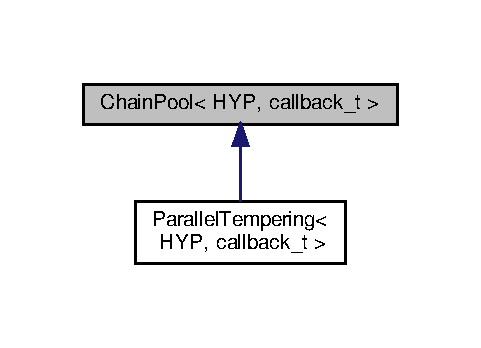
\includegraphics[width=231pt]{class_chain_pool__inherit__graph}
\end{center}
\end{figure}
\subsection*{Public Member Functions}
\begin{DoxyCompactItemize}
\item 
\hyperlink{class_chain_pool_ae8795a9a7c0fff45c82334fa821c8c3c}{Chain\+Pool} ()
\item 
\hyperlink{class_chain_pool_ae6d9483840ee517354d429324fbcc800}{Chain\+Pool} (H\+YP \&h0, typename H\+Y\+P\+::t\+\_\+data $\ast$d, callback\+\_\+t \&cb, size\+\_\+t n, bool allcallback=true)
\item 
virtual void \hyperlink{class_chain_pool_af5f0e391f9794ff89f29296c8b41bf8e}{run} (\hyperlink{struct_control}{Control} ctl)
\end{DoxyCompactItemize}
\subsection*{Static Public Member Functions}
\begin{DoxyCompactItemize}
\item 
static void \hyperlink{class_chain_pool_a7df513bcd7b99c2fa99a9cfdd238817b}{\+\_\+\+\_\+run\+\_\+helper} (std\+::vector$<$ \hyperlink{class_m_c_m_c_chain}{M\+C\+M\+C\+Chain}$<$ H\+YP, callback\+\_\+t $>$$>$ $\ast$\hyperlink{class_chain_pool_af89400f6e9a2312fe2ee7873745a6e91}{pool}, std\+::vector$<$ bool $>$ $\ast$running, std\+::mutex $\ast$\hyperlink{class_chain_pool_a6efe006156a22132b452d50dab9f76c0}{running\+\_\+mutex}, \hyperlink{struct_control}{Control} ctl)
\end{DoxyCompactItemize}
\subsection*{Public Attributes}
\begin{DoxyCompactItemize}
\item 
std\+::vector$<$ \hyperlink{class_m_c_m_c_chain}{M\+C\+M\+C\+Chain}$<$ H\+YP, callback\+\_\+t $>$ $>$ \hyperlink{class_chain_pool_af89400f6e9a2312fe2ee7873745a6e91}{pool}
\item 
std\+::mutex \hyperlink{class_chain_pool_a6efe006156a22132b452d50dab9f76c0}{running\+\_\+mutex}
\end{DoxyCompactItemize}
\subsection*{Static Public Attributes}
\begin{DoxyCompactItemize}
\item 
static const unsigned long \hyperlink{class_chain_pool_a143f3e4f9b60c03c67ffbc2db3e57d53}{steps\+\_\+before\+\_\+change} = 0
\item 
static const time\+\_\+ms \hyperlink{class_chain_pool_a1ff48aa1e09a9a31871dec05d3c0e9d3}{time\+\_\+before\+\_\+change} = 250
\end{DoxyCompactItemize}


\subsection{Detailed Description}
\subsubsection*{template$<$typename H\+YP, typename callback\+\_\+t$>$\newline
class Chain\+Pool$<$ H\+Y\+P, callback\+\_\+t $>$}

\begin{DoxyAuthor}{Author}
steven piantadosi 
\end{DoxyAuthor}
\begin{DoxyDate}{Date}
29/01/20 
\end{DoxyDate}


\subsection{Constructor \& Destructor Documentation}
\mbox{\Hypertarget{class_chain_pool_ae8795a9a7c0fff45c82334fa821c8c3c}\label{class_chain_pool_ae8795a9a7c0fff45c82334fa821c8c3c}} 
\index{Chain\+Pool@{Chain\+Pool}!Chain\+Pool@{Chain\+Pool}}
\index{Chain\+Pool@{Chain\+Pool}!Chain\+Pool@{Chain\+Pool}}
\subsubsection{\texorpdfstring{Chain\+Pool()}{ChainPool()}\hspace{0.1cm}{\footnotesize\ttfamily [1/2]}}
{\footnotesize\ttfamily template$<$typename H\+YP , typename callback\+\_\+t $>$ \\
\hyperlink{class_chain_pool}{Chain\+Pool}$<$ H\+YP, callback\+\_\+t $>$\+::\hyperlink{class_chain_pool}{Chain\+Pool} (\begin{DoxyParamCaption}{ }\end{DoxyParamCaption})\hspace{0.3cm}{\ttfamily [inline]}}

\mbox{\Hypertarget{class_chain_pool_ae6d9483840ee517354d429324fbcc800}\label{class_chain_pool_ae6d9483840ee517354d429324fbcc800}} 
\index{Chain\+Pool@{Chain\+Pool}!Chain\+Pool@{Chain\+Pool}}
\index{Chain\+Pool@{Chain\+Pool}!Chain\+Pool@{Chain\+Pool}}
\subsubsection{\texorpdfstring{Chain\+Pool()}{ChainPool()}\hspace{0.1cm}{\footnotesize\ttfamily [2/2]}}
{\footnotesize\ttfamily template$<$typename H\+YP , typename callback\+\_\+t $>$ \\
\hyperlink{class_chain_pool}{Chain\+Pool}$<$ H\+YP, callback\+\_\+t $>$\+::\hyperlink{class_chain_pool}{Chain\+Pool} (\begin{DoxyParamCaption}\item[{H\+YP \&}]{h0,  }\item[{typename H\+Y\+P\+::t\+\_\+data $\ast$}]{d,  }\item[{callback\+\_\+t \&}]{cb,  }\item[{size\+\_\+t}]{n,  }\item[{bool}]{allcallback = {\ttfamily true} }\end{DoxyParamCaption})\hspace{0.3cm}{\ttfamily [inline]}}



\subsection{Member Function Documentation}
\mbox{\Hypertarget{class_chain_pool_a7df513bcd7b99c2fa99a9cfdd238817b}\label{class_chain_pool_a7df513bcd7b99c2fa99a9cfdd238817b}} 
\index{Chain\+Pool@{Chain\+Pool}!\+\_\+\+\_\+run\+\_\+helper@{\+\_\+\+\_\+run\+\_\+helper}}
\index{\+\_\+\+\_\+run\+\_\+helper@{\+\_\+\+\_\+run\+\_\+helper}!Chain\+Pool@{Chain\+Pool}}
\subsubsection{\texorpdfstring{\+\_\+\+\_\+run\+\_\+helper()}{\_\_run\_helper()}}
{\footnotesize\ttfamily template$<$typename H\+YP , typename callback\+\_\+t $>$ \\
static void \hyperlink{class_chain_pool}{Chain\+Pool}$<$ H\+YP, callback\+\_\+t $>$\+::\+\_\+\+\_\+run\+\_\+helper (\begin{DoxyParamCaption}\item[{std\+::vector$<$ \hyperlink{class_m_c_m_c_chain}{M\+C\+M\+C\+Chain}$<$ H\+YP, callback\+\_\+t $>$$>$ $\ast$}]{pool,  }\item[{std\+::vector$<$ bool $>$ $\ast$}]{running,  }\item[{std\+::mutex $\ast$}]{running\+\_\+mutex,  }\item[{\hyperlink{struct_control}{Control}}]{ctl }\end{DoxyParamCaption})\hspace{0.3cm}{\ttfamily [inline]}, {\ttfamily [static]}}

This run helper is called internally by multiple different threads, and runs a given pool. 
\begin{DoxyParams}{Parameters}
{\em ctl} & \\
\hline
\end{DoxyParams}
\mbox{\Hypertarget{class_chain_pool_af5f0e391f9794ff89f29296c8b41bf8e}\label{class_chain_pool_af5f0e391f9794ff89f29296c8b41bf8e}} 
\index{Chain\+Pool@{Chain\+Pool}!run@{run}}
\index{run@{run}!Chain\+Pool@{Chain\+Pool}}
\subsubsection{\texorpdfstring{run()}{run()}}
{\footnotesize\ttfamily template$<$typename H\+YP , typename callback\+\_\+t $>$ \\
virtual void \hyperlink{class_chain_pool}{Chain\+Pool}$<$ H\+YP, callback\+\_\+t $>$\+::run (\begin{DoxyParamCaption}\item[{\hyperlink{struct_control}{Control}}]{ctl }\end{DoxyParamCaption})\hspace{0.3cm}{\ttfamily [inline]}, {\ttfamily [virtual]}}



Reimplemented in \hyperlink{class_parallel_tempering_a6824837893cf52eb1cac362e78e483b9}{Parallel\+Tempering$<$ H\+Y\+P, callback\+\_\+t $>$}.



\subsection{Member Data Documentation}
\mbox{\Hypertarget{class_chain_pool_af89400f6e9a2312fe2ee7873745a6e91}\label{class_chain_pool_af89400f6e9a2312fe2ee7873745a6e91}} 
\index{Chain\+Pool@{Chain\+Pool}!pool@{pool}}
\index{pool@{pool}!Chain\+Pool@{Chain\+Pool}}
\subsubsection{\texorpdfstring{pool}{pool}}
{\footnotesize\ttfamily template$<$typename H\+YP , typename callback\+\_\+t $>$ \\
std\+::vector$<$\hyperlink{class_m_c_m_c_chain}{M\+C\+M\+C\+Chain}$<$H\+YP,callback\+\_\+t$>$ $>$ \hyperlink{class_chain_pool}{Chain\+Pool}$<$ H\+YP, callback\+\_\+t $>$\+::pool}

\mbox{\Hypertarget{class_chain_pool_a6efe006156a22132b452d50dab9f76c0}\label{class_chain_pool_a6efe006156a22132b452d50dab9f76c0}} 
\index{Chain\+Pool@{Chain\+Pool}!running\+\_\+mutex@{running\+\_\+mutex}}
\index{running\+\_\+mutex@{running\+\_\+mutex}!Chain\+Pool@{Chain\+Pool}}
\subsubsection{\texorpdfstring{running\+\_\+mutex}{running\_mutex}}
{\footnotesize\ttfamily template$<$typename H\+YP , typename callback\+\_\+t $>$ \\
std\+::mutex \hyperlink{class_chain_pool}{Chain\+Pool}$<$ H\+YP, callback\+\_\+t $>$\+::running\+\_\+mutex}

\mbox{\Hypertarget{class_chain_pool_a143f3e4f9b60c03c67ffbc2db3e57d53}\label{class_chain_pool_a143f3e4f9b60c03c67ffbc2db3e57d53}} 
\index{Chain\+Pool@{Chain\+Pool}!steps\+\_\+before\+\_\+change@{steps\+\_\+before\+\_\+change}}
\index{steps\+\_\+before\+\_\+change@{steps\+\_\+before\+\_\+change}!Chain\+Pool@{Chain\+Pool}}
\subsubsection{\texorpdfstring{steps\+\_\+before\+\_\+change}{steps\_before\_change}}
{\footnotesize\ttfamily template$<$typename H\+YP , typename callback\+\_\+t $>$ \\
const unsigned long \hyperlink{class_chain_pool}{Chain\+Pool}$<$ H\+YP, callback\+\_\+t $>$\+::steps\+\_\+before\+\_\+change = 0\hspace{0.3cm}{\ttfamily [static]}}

\mbox{\Hypertarget{class_chain_pool_a1ff48aa1e09a9a31871dec05d3c0e9d3}\label{class_chain_pool_a1ff48aa1e09a9a31871dec05d3c0e9d3}} 
\index{Chain\+Pool@{Chain\+Pool}!time\+\_\+before\+\_\+change@{time\+\_\+before\+\_\+change}}
\index{time\+\_\+before\+\_\+change@{time\+\_\+before\+\_\+change}!Chain\+Pool@{Chain\+Pool}}
\subsubsection{\texorpdfstring{time\+\_\+before\+\_\+change}{time\_before\_change}}
{\footnotesize\ttfamily template$<$typename H\+YP , typename callback\+\_\+t $>$ \\
const time\+\_\+ms \hyperlink{class_chain_pool}{Chain\+Pool}$<$ H\+YP, callback\+\_\+t $>$\+::time\+\_\+before\+\_\+change = 250\hspace{0.3cm}{\ttfamily [static]}}



The documentation for this class was generated from the following file\+:\begin{DoxyCompactItemize}
\item 
src/\+Inference/\hyperlink{_chain_pool_8h}{Chain\+Pool.\+h}\end{DoxyCompactItemize}

\input{struct_check_reference_is_first}
\input{struct_check_reference_is_first_3_01_t_01_4}
\hypertarget{struct_control}{}\section{Control Class Reference}
\label{struct_control}\index{Control@{Control}}


{\ttfamily \#include $<$Control.\+h$>$}

\subsection*{Public Member Functions}
\begin{DoxyCompactItemize}
\item 
\hyperlink{struct_control_a4ff9d1cb18c06b5438f09ef6a8e7af80}{Control} (unsigned long s=0, time\+\_\+ms t=0, size\+\_\+t thr=1, unsigned long r=0)
\item 
void \hyperlink{struct_control_a933994a3524f2f6d7ef0a17086e7cf66}{start} ()
\item 
bool \hyperlink{struct_control_a9217475a8ad619e7360524ae49c559a7}{running} ()
\end{DoxyCompactItemize}
\subsection*{Public Attributes}
\begin{DoxyCompactItemize}
\item 
unsigned long \hyperlink{struct_control_af4bd5a6c779079b5e921b4df40760266}{steps}
\item 
time\+\_\+ms \hyperlink{struct_control_a273f3488d567bb10871e71245a406f3e}{time}
\item 
size\+\_\+t \hyperlink{struct_control_af130110f07dc3bced4d8d0fafac5b755}{threads}
\item 
unsigned long \hyperlink{struct_control_acb1e669784385d64b9f840674a3e08c1}{burn}
\item 
unsigned long \hyperlink{struct_control_a08030350e86fd21411599690892e31a8}{thin}
\item 
unsigned long \hyperlink{struct_control_acd75b8aa48fdb33f063bae7469a9721b}{restart}
\item 
timept \hyperlink{struct_control_ad3c2691a66705880844f467cf5da8aab}{start\+\_\+time}
\item 
unsigned long \hyperlink{struct_control_a4a1867401c3e89aecaf14949521ed247}{done\+\_\+steps}
\item 
bool \hyperlink{struct_control_a3a1856c582efd2a6a1b8f40351038d0c}{break\+\_\+\+C\+T\+R\+LC}
\end{DoxyCompactItemize}


\subsection{Detailed Description}
\begin{DoxyAuthor}{Author}
steven piantadosi 
\end{DoxyAuthor}
\begin{DoxyDate}{Date}
03/02/20 
\end{DoxyDate}


\subsection{Constructor \& Destructor Documentation}
\mbox{\Hypertarget{struct_control_a4ff9d1cb18c06b5438f09ef6a8e7af80}\label{struct_control_a4ff9d1cb18c06b5438f09ef6a8e7af80}} 
\index{Control@{Control}!Control@{Control}}
\index{Control@{Control}!Control@{Control}}
\subsubsection{\texorpdfstring{Control()}{Control()}}
{\footnotesize\ttfamily Control\+::\+Control (\begin{DoxyParamCaption}\item[{unsigned long}]{s = {\ttfamily 0},  }\item[{time\+\_\+ms}]{t = {\ttfamily 0},  }\item[{size\+\_\+t}]{thr = {\ttfamily 1},  }\item[{unsigned long}]{r = {\ttfamily 0} }\end{DoxyParamCaption})\hspace{0.3cm}{\ttfamily [inline]}}



\subsection{Member Function Documentation}
\mbox{\Hypertarget{struct_control_a9217475a8ad619e7360524ae49c559a7}\label{struct_control_a9217475a8ad619e7360524ae49c559a7}} 
\index{Control@{Control}!running@{running}}
\index{running@{running}!Control@{Control}}
\subsubsection{\texorpdfstring{running()}{running()}}
{\footnotesize\ttfamily bool Control\+::running (\begin{DoxyParamCaption}{ }\end{DoxyParamCaption})\hspace{0.3cm}{\ttfamily [inline]}}

Check if we are currently running. \begin{DoxyReturn}{Returns}

\end{DoxyReturn}
\mbox{\Hypertarget{struct_control_a933994a3524f2f6d7ef0a17086e7cf66}\label{struct_control_a933994a3524f2f6d7ef0a17086e7cf66}} 
\index{Control@{Control}!start@{start}}
\index{start@{start}!Control@{Control}}
\subsubsection{\texorpdfstring{start()}{start()}}
{\footnotesize\ttfamily void Control\+::start (\begin{DoxyParamCaption}{ }\end{DoxyParamCaption})\hspace{0.3cm}{\ttfamily [inline]}}

Start running

\subsection{Member Data Documentation}
\mbox{\Hypertarget{struct_control_a3a1856c582efd2a6a1b8f40351038d0c}\label{struct_control_a3a1856c582efd2a6a1b8f40351038d0c}} 
\index{Control@{Control}!break\+\_\+\+C\+T\+R\+LC@{break\+\_\+\+C\+T\+R\+LC}}
\index{break\+\_\+\+C\+T\+R\+LC@{break\+\_\+\+C\+T\+R\+LC}!Control@{Control}}
\subsubsection{\texorpdfstring{break\+\_\+\+C\+T\+R\+LC}{break\_CTRLC}}
{\footnotesize\ttfamily bool Control\+::break\+\_\+\+C\+T\+R\+LC}

\mbox{\Hypertarget{struct_control_acb1e669784385d64b9f840674a3e08c1}\label{struct_control_acb1e669784385d64b9f840674a3e08c1}} 
\index{Control@{Control}!burn@{burn}}
\index{burn@{burn}!Control@{Control}}
\subsubsection{\texorpdfstring{burn}{burn}}
{\footnotesize\ttfamily unsigned long Control\+::burn}

\mbox{\Hypertarget{struct_control_a4a1867401c3e89aecaf14949521ed247}\label{struct_control_a4a1867401c3e89aecaf14949521ed247}} 
\index{Control@{Control}!done\+\_\+steps@{done\+\_\+steps}}
\index{done\+\_\+steps@{done\+\_\+steps}!Control@{Control}}
\subsubsection{\texorpdfstring{done\+\_\+steps}{done\_steps}}
{\footnotesize\ttfamily unsigned long Control\+::done\+\_\+steps}

\mbox{\Hypertarget{struct_control_acd75b8aa48fdb33f063bae7469a9721b}\label{struct_control_acd75b8aa48fdb33f063bae7469a9721b}} 
\index{Control@{Control}!restart@{restart}}
\index{restart@{restart}!Control@{Control}}
\subsubsection{\texorpdfstring{restart}{restart}}
{\footnotesize\ttfamily unsigned long Control\+::restart}

\mbox{\Hypertarget{struct_control_ad3c2691a66705880844f467cf5da8aab}\label{struct_control_ad3c2691a66705880844f467cf5da8aab}} 
\index{Control@{Control}!start\+\_\+time@{start\+\_\+time}}
\index{start\+\_\+time@{start\+\_\+time}!Control@{Control}}
\subsubsection{\texorpdfstring{start\+\_\+time}{start\_time}}
{\footnotesize\ttfamily timept Control\+::start\+\_\+time}

\mbox{\Hypertarget{struct_control_af4bd5a6c779079b5e921b4df40760266}\label{struct_control_af4bd5a6c779079b5e921b4df40760266}} 
\index{Control@{Control}!steps@{steps}}
\index{steps@{steps}!Control@{Control}}
\subsubsection{\texorpdfstring{steps}{steps}}
{\footnotesize\ttfamily unsigned long Control\+::steps}

\mbox{\Hypertarget{struct_control_a08030350e86fd21411599690892e31a8}\label{struct_control_a08030350e86fd21411599690892e31a8}} 
\index{Control@{Control}!thin@{thin}}
\index{thin@{thin}!Control@{Control}}
\subsubsection{\texorpdfstring{thin}{thin}}
{\footnotesize\ttfamily unsigned long Control\+::thin}

\mbox{\Hypertarget{struct_control_af130110f07dc3bced4d8d0fafac5b755}\label{struct_control_af130110f07dc3bced4d8d0fafac5b755}} 
\index{Control@{Control}!threads@{threads}}
\index{threads@{threads}!Control@{Control}}
\subsubsection{\texorpdfstring{threads}{threads}}
{\footnotesize\ttfamily size\+\_\+t Control\+::threads}

\mbox{\Hypertarget{struct_control_a273f3488d567bb10871e71245a406f3e}\label{struct_control_a273f3488d567bb10871e71245a406f3e}} 
\index{Control@{Control}!time@{time}}
\index{time@{time}!Control@{Control}}
\subsubsection{\texorpdfstring{time}{time}}
{\footnotesize\ttfamily time\+\_\+ms Control\+::time}



The documentation for this class was generated from the following file\+:\begin{DoxyCompactItemize}
\item 
src/\hyperlink{_control_8h}{Control.\+h}\end{DoxyCompactItemize}

\input{struct_count_references}
\input{struct_count_references_3_01_t_01_4}
\hypertarget{classdefault__datum}{}\section{default\+\_\+datum$<$ t\+\_\+input, t\+\_\+output $>$ Class Template Reference}
\label{classdefault__datum}\index{default\+\_\+datum$<$ t\+\_\+input, t\+\_\+output $>$@{default\+\_\+datum$<$ t\+\_\+input, t\+\_\+output $>$}}


{\ttfamily \#include $<$Datum.\+h$>$}

\subsection*{Public Member Functions}
\begin{DoxyCompactItemize}
\item 
\hyperlink{classdefault__datum_a7153b5621e08e438753c4a90271c2eee}{default\+\_\+datum} ()
\item 
\hyperlink{classdefault__datum_aaaa9c76cb8d02eab61cc6f0c3570a64d}{default\+\_\+datum} (const t\+\_\+input \&i, const t\+\_\+output \&o, double r)
\item 
\hyperlink{classdefault__datum_aab82d7d96c8fdcecc36b554b83a5e5e2}{default\+\_\+datum} (const t\+\_\+input \&i, const t\+\_\+output \&o)
\item 
bool \hyperlink{classdefault__datum_a1da1cd62c4b98771b010d5b625c2f744}{operator==} (const \hyperlink{classdefault__datum}{default\+\_\+datum} \&y) const
\end{DoxyCompactItemize}
\subsection*{Public Attributes}
\begin{DoxyCompactItemize}
\item 
t\+\_\+input \hyperlink{classdefault__datum_a19f8427ac058ad008f5b2541e17d42e7}{input}
\item 
t\+\_\+output \hyperlink{classdefault__datum_afafbe2c709ff57daca0fd60289bdd13a}{output}
\item 
double \hyperlink{classdefault__datum_ad9d6b81d35ca8107e8c810186cef9270}{reliability}
\end{DoxyCompactItemize}


\subsection{Detailed Description}
\subsubsection*{template$<$typename t\+\_\+input, typename t\+\_\+output$>$\newline
class default\+\_\+datum$<$ t\+\_\+input, t\+\_\+output $>$}

\begin{DoxyAuthor}{Author}
piantado 
\end{DoxyAuthor}
\begin{DoxyDate}{Date}
29/01/20 
\end{DoxyDate}


\subsection{Constructor \& Destructor Documentation}
\mbox{\Hypertarget{classdefault__datum_a7153b5621e08e438753c4a90271c2eee}\label{classdefault__datum_a7153b5621e08e438753c4a90271c2eee}} 
\index{default\+\_\+datum@{default\+\_\+datum}!default\+\_\+datum@{default\+\_\+datum}}
\index{default\+\_\+datum@{default\+\_\+datum}!default\+\_\+datum@{default\+\_\+datum}}
\subsubsection{\texorpdfstring{default\+\_\+datum()}{default\_datum()}\hspace{0.1cm}{\footnotesize\ttfamily [1/3]}}
{\footnotesize\ttfamily template$<$typename t\+\_\+input, typename t\+\_\+output$>$ \\
\hyperlink{classdefault__datum}{default\+\_\+datum}$<$ t\+\_\+input, t\+\_\+output $>$\+::\hyperlink{classdefault__datum}{default\+\_\+datum} (\begin{DoxyParamCaption}{ }\end{DoxyParamCaption})\hspace{0.3cm}{\ttfamily [inline]}}

\mbox{\Hypertarget{classdefault__datum_aaaa9c76cb8d02eab61cc6f0c3570a64d}\label{classdefault__datum_aaaa9c76cb8d02eab61cc6f0c3570a64d}} 
\index{default\+\_\+datum@{default\+\_\+datum}!default\+\_\+datum@{default\+\_\+datum}}
\index{default\+\_\+datum@{default\+\_\+datum}!default\+\_\+datum@{default\+\_\+datum}}
\subsubsection{\texorpdfstring{default\+\_\+datum()}{default\_datum()}\hspace{0.1cm}{\footnotesize\ttfamily [2/3]}}
{\footnotesize\ttfamily template$<$typename t\+\_\+input, typename t\+\_\+output$>$ \\
\hyperlink{classdefault__datum}{default\+\_\+datum}$<$ t\+\_\+input, t\+\_\+output $>$\+::\hyperlink{classdefault__datum}{default\+\_\+datum} (\begin{DoxyParamCaption}\item[{const t\+\_\+input \&}]{i,  }\item[{const t\+\_\+output \&}]{o,  }\item[{double}]{r }\end{DoxyParamCaption})\hspace{0.3cm}{\ttfamily [inline]}}

\mbox{\Hypertarget{classdefault__datum_aab82d7d96c8fdcecc36b554b83a5e5e2}\label{classdefault__datum_aab82d7d96c8fdcecc36b554b83a5e5e2}} 
\index{default\+\_\+datum@{default\+\_\+datum}!default\+\_\+datum@{default\+\_\+datum}}
\index{default\+\_\+datum@{default\+\_\+datum}!default\+\_\+datum@{default\+\_\+datum}}
\subsubsection{\texorpdfstring{default\+\_\+datum()}{default\_datum()}\hspace{0.1cm}{\footnotesize\ttfamily [3/3]}}
{\footnotesize\ttfamily template$<$typename t\+\_\+input, typename t\+\_\+output$>$ \\
\hyperlink{classdefault__datum}{default\+\_\+datum}$<$ t\+\_\+input, t\+\_\+output $>$\+::\hyperlink{classdefault__datum}{default\+\_\+datum} (\begin{DoxyParamCaption}\item[{const t\+\_\+input \&}]{i,  }\item[{const t\+\_\+output \&}]{o }\end{DoxyParamCaption})\hspace{0.3cm}{\ttfamily [inline]}}



\subsection{Member Function Documentation}
\mbox{\Hypertarget{classdefault__datum_a1da1cd62c4b98771b010d5b625c2f744}\label{classdefault__datum_a1da1cd62c4b98771b010d5b625c2f744}} 
\index{default\+\_\+datum@{default\+\_\+datum}!operator==@{operator==}}
\index{operator==@{operator==}!default\+\_\+datum@{default\+\_\+datum}}
\subsubsection{\texorpdfstring{operator==()}{operator==()}}
{\footnotesize\ttfamily template$<$typename t\+\_\+input, typename t\+\_\+output$>$ \\
bool \hyperlink{classdefault__datum}{default\+\_\+datum}$<$ t\+\_\+input, t\+\_\+output $>$\+::operator== (\begin{DoxyParamCaption}\item[{const \hyperlink{classdefault__datum}{default\+\_\+datum}$<$ t\+\_\+input, t\+\_\+output $>$ \&}]{y }\end{DoxyParamCaption}) const\hspace{0.3cm}{\ttfamily [inline]}}



\subsection{Member Data Documentation}
\mbox{\Hypertarget{classdefault__datum_a19f8427ac058ad008f5b2541e17d42e7}\label{classdefault__datum_a19f8427ac058ad008f5b2541e17d42e7}} 
\index{default\+\_\+datum@{default\+\_\+datum}!input@{input}}
\index{input@{input}!default\+\_\+datum@{default\+\_\+datum}}
\subsubsection{\texorpdfstring{input}{input}}
{\footnotesize\ttfamily template$<$typename t\+\_\+input, typename t\+\_\+output$>$ \\
t\+\_\+input \hyperlink{classdefault__datum}{default\+\_\+datum}$<$ t\+\_\+input, t\+\_\+output $>$\+::input}

\mbox{\Hypertarget{classdefault__datum_afafbe2c709ff57daca0fd60289bdd13a}\label{classdefault__datum_afafbe2c709ff57daca0fd60289bdd13a}} 
\index{default\+\_\+datum@{default\+\_\+datum}!output@{output}}
\index{output@{output}!default\+\_\+datum@{default\+\_\+datum}}
\subsubsection{\texorpdfstring{output}{output}}
{\footnotesize\ttfamily template$<$typename t\+\_\+input, typename t\+\_\+output$>$ \\
t\+\_\+output \hyperlink{classdefault__datum}{default\+\_\+datum}$<$ t\+\_\+input, t\+\_\+output $>$\+::output}

\mbox{\Hypertarget{classdefault__datum_ad9d6b81d35ca8107e8c810186cef9270}\label{classdefault__datum_ad9d6b81d35ca8107e8c810186cef9270}} 
\index{default\+\_\+datum@{default\+\_\+datum}!reliability@{reliability}}
\index{reliability@{reliability}!default\+\_\+datum@{default\+\_\+datum}}
\subsubsection{\texorpdfstring{reliability}{reliability}}
{\footnotesize\ttfamily template$<$typename t\+\_\+input, typename t\+\_\+output$>$ \\
double \hyperlink{classdefault__datum}{default\+\_\+datum}$<$ t\+\_\+input, t\+\_\+output $>$\+::reliability}



The documentation for this class was generated from the following file\+:\begin{DoxyCompactItemize}
\item 
src/\+Hypotheses/\hyperlink{_datum_8h}{Datum.\+h}\end{DoxyCompactItemize}

\hypertarget{class_depth_exception}{}\section{Depth\+Exception Class Reference}
\label{class_depth_exception}\index{Depth\+Exception@{Depth\+Exception}}


{\ttfamily \#include $<$Grammar.\+h$>$}



Inheritance diagram for Depth\+Exception\+:\nopagebreak
\begin{figure}[H]
\begin{center}
\leavevmode
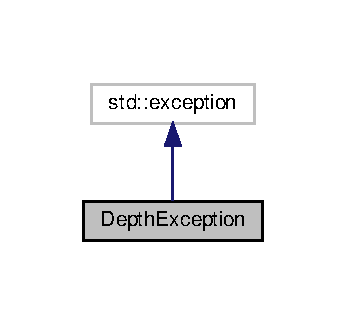
\includegraphics[width=166pt]{class_depth_exception__inherit__graph}
\end{center}
\end{figure}


Collaboration diagram for Depth\+Exception\+:\nopagebreak
\begin{figure}[H]
\begin{center}
\leavevmode
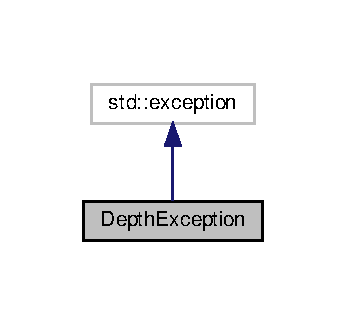
\includegraphics[width=166pt]{class_depth_exception__coll__graph}
\end{center}
\end{figure}


The documentation for this class was generated from the following file\+:\begin{DoxyCompactItemize}
\item 
src/\hyperlink{_grammar_8h}{Grammar.\+h}\end{DoxyCompactItemize}

\hypertarget{class_discrete_distribution}{}\section{Discrete\+Distribution$<$ T $>$ Class Template Reference}
\label{class_discrete_distribution}\index{Discrete\+Distribution$<$ T $>$@{Discrete\+Distribution$<$ T $>$}}


{\ttfamily \#include $<$Discrete\+Distribution.\+h$>$}

\subsection*{Public Member Functions}
\begin{DoxyCompactItemize}
\item 
\hyperlink{class_discrete_distribution_a8ffb7c55f85cf42af7aec6deb97ec4ab}{Discrete\+Distribution} ()
\item 
virtual T \hyperlink{class_discrete_distribution_a7cf660223fe0f86b61e3b33268204c06}{argmax} () const
\item 
void \hyperlink{class_discrete_distribution_a6ec6f590a3659c8bef32aaab77a8052e}{print} (std\+::ostream \&out, unsigned long nprint=0) const
\item 
void \hyperlink{class_discrete_distribution_a58bc689015e6b594ed1a53130758ba6f}{print} (unsigned long nprint=0) const
\item 
std\+::string \hyperlink{class_discrete_distribution_a87d866919f4698e488aee9ce4bc42ed5}{string} (unsigned long nprint=0) const
\item 
void \hyperlink{class_discrete_distribution_a6c41c7f4726019bc213d37d4e3cdea27}{addmass} (T x, double v)
\item 
const std\+::map$<$ T, double $>$ \& \hyperlink{class_discrete_distribution_a995377a760a6fe0d44077892053acdbb}{values} () const
\item 
void \hyperlink{class_discrete_distribution_a5c93983e2375a2353b10b82ebb11f751}{operator$<$$<$} (const \hyperlink{class_discrete_distribution}{Discrete\+Distribution}$<$ T $>$ \&x)
\item 
std\+::vector$<$ T $>$ \hyperlink{class_discrete_distribution_adee72a8e4c93aa03d841c0c73d6b5498}{best} (size\+\_\+t N) const
\item 
std\+::vector$<$ std\+::pair$<$ T, double $>$ $>$ \hyperlink{class_discrete_distribution_a94488cfd094f6cde47f15a1f4c7cdbb9}{sorted} (bool decreasing=false) const
\item 
size\+\_\+t \hyperlink{class_discrete_distribution_afd3fd83dc776f5616e826de18093328b}{count} (T x) const
\item 
size\+\_\+t \hyperlink{class_discrete_distribution_ad74207d32c2ed6c5c26b3f991f4fedba}{size} () const
\item 
double \hyperlink{class_discrete_distribution_aa06afa5c16edf065b1567ea7b6b4356a}{operator\mbox{[}$\,$\mbox{]}} (T x)
\item 
double \hyperlink{class_discrete_distribution_acb11f1cfbf4ef039c538f06cde8249fd}{at} (T x) const
\end{DoxyCompactItemize}
\subsection*{Public Attributes}
\begin{DoxyCompactItemize}
\item 
std\+::map$<$ T, double $>$ \hyperlink{class_discrete_distribution_a72a09b5b79a5bf0c55f780b9a81271fb}{m}
\end{DoxyCompactItemize}


\subsection{Detailed Description}
\subsubsection*{template$<$typename T$>$\newline
class Discrete\+Distribution$<$ T $>$}

\begin{DoxyAuthor}{Author}
steven piantadosi 
\end{DoxyAuthor}
\begin{DoxyDate}{Date}
03/02/20 
\end{DoxyDate}


\subsection{Constructor \& Destructor Documentation}
\mbox{\Hypertarget{class_discrete_distribution_a8ffb7c55f85cf42af7aec6deb97ec4ab}\label{class_discrete_distribution_a8ffb7c55f85cf42af7aec6deb97ec4ab}} 
\index{Discrete\+Distribution@{Discrete\+Distribution}!Discrete\+Distribution@{Discrete\+Distribution}}
\index{Discrete\+Distribution@{Discrete\+Distribution}!Discrete\+Distribution@{Discrete\+Distribution}}
\subsubsection{\texorpdfstring{Discrete\+Distribution()}{DiscreteDistribution()}}
{\footnotesize\ttfamily template$<$typename T$>$ \\
\hyperlink{class_discrete_distribution}{Discrete\+Distribution}$<$ T $>$\+::\hyperlink{class_discrete_distribution}{Discrete\+Distribution} (\begin{DoxyParamCaption}{ }\end{DoxyParamCaption})\hspace{0.3cm}{\ttfamily [inline]}}



\subsection{Member Function Documentation}
\mbox{\Hypertarget{class_discrete_distribution_a6c41c7f4726019bc213d37d4e3cdea27}\label{class_discrete_distribution_a6c41c7f4726019bc213d37d4e3cdea27}} 
\index{Discrete\+Distribution@{Discrete\+Distribution}!addmass@{addmass}}
\index{addmass@{addmass}!Discrete\+Distribution@{Discrete\+Distribution}}
\subsubsection{\texorpdfstring{addmass()}{addmass()}}
{\footnotesize\ttfamily template$<$typename T$>$ \\
void \hyperlink{class_discrete_distribution}{Discrete\+Distribution}$<$ T $>$\+::addmass (\begin{DoxyParamCaption}\item[{T}]{x,  }\item[{double}]{v }\end{DoxyParamCaption})\hspace{0.3cm}{\ttfamily [inline]}}

Add log probability v to type x 
\begin{DoxyParams}{Parameters}
{\em x} & \\
\hline
{\em v} & \\
\hline
\end{DoxyParams}
\mbox{\Hypertarget{class_discrete_distribution_a7cf660223fe0f86b61e3b33268204c06}\label{class_discrete_distribution_a7cf660223fe0f86b61e3b33268204c06}} 
\index{Discrete\+Distribution@{Discrete\+Distribution}!argmax@{argmax}}
\index{argmax@{argmax}!Discrete\+Distribution@{Discrete\+Distribution}}
\subsubsection{\texorpdfstring{argmax()}{argmax()}}
{\footnotesize\ttfamily template$<$typename T$>$ \\
virtual T \hyperlink{class_discrete_distribution}{Discrete\+Distribution}$<$ T $>$\+::argmax (\begin{DoxyParamCaption}{ }\end{DoxyParamCaption}) const\hspace{0.3cm}{\ttfamily [inline]}, {\ttfamily [virtual]}}

\mbox{\Hypertarget{class_discrete_distribution_acb11f1cfbf4ef039c538f06cde8249fd}\label{class_discrete_distribution_acb11f1cfbf4ef039c538f06cde8249fd}} 
\index{Discrete\+Distribution@{Discrete\+Distribution}!at@{at}}
\index{at@{at}!Discrete\+Distribution@{Discrete\+Distribution}}
\subsubsection{\texorpdfstring{at()}{at()}}
{\footnotesize\ttfamily template$<$typename T$>$ \\
double \hyperlink{class_discrete_distribution}{Discrete\+Distribution}$<$ T $>$\+::at (\begin{DoxyParamCaption}\item[{T}]{x }\end{DoxyParamCaption}) const\hspace{0.3cm}{\ttfamily [inline]}}

\mbox{\Hypertarget{class_discrete_distribution_adee72a8e4c93aa03d841c0c73d6b5498}\label{class_discrete_distribution_adee72a8e4c93aa03d841c0c73d6b5498}} 
\index{Discrete\+Distribution@{Discrete\+Distribution}!best@{best}}
\index{best@{best}!Discrete\+Distribution@{Discrete\+Distribution}}
\subsubsection{\texorpdfstring{best()}{best()}}
{\footnotesize\ttfamily template$<$typename T$>$ \\
std\+::vector$<$T$>$ \hyperlink{class_discrete_distribution}{Discrete\+Distribution}$<$ T $>$\+::best (\begin{DoxyParamCaption}\item[{size\+\_\+t}]{N }\end{DoxyParamCaption}) const\hspace{0.3cm}{\ttfamily [inline]}}

Get the N best from this distribution 
\begin{DoxyParams}{Parameters}
{\em N} & \\
\hline
\end{DoxyParams}
\begin{DoxyReturn}{Returns}

\end{DoxyReturn}
\mbox{\Hypertarget{class_discrete_distribution_afd3fd83dc776f5616e826de18093328b}\label{class_discrete_distribution_afd3fd83dc776f5616e826de18093328b}} 
\index{Discrete\+Distribution@{Discrete\+Distribution}!count@{count}}
\index{count@{count}!Discrete\+Distribution@{Discrete\+Distribution}}
\subsubsection{\texorpdfstring{count()}{count()}}
{\footnotesize\ttfamily template$<$typename T$>$ \\
size\+\_\+t \hyperlink{class_discrete_distribution}{Discrete\+Distribution}$<$ T $>$\+::count (\begin{DoxyParamCaption}\item[{T}]{x }\end{DoxyParamCaption}) const\hspace{0.3cm}{\ttfamily [inline]}}

\mbox{\Hypertarget{class_discrete_distribution_a5c93983e2375a2353b10b82ebb11f751}\label{class_discrete_distribution_a5c93983e2375a2353b10b82ebb11f751}} 
\index{Discrete\+Distribution@{Discrete\+Distribution}!operator$<$$<$@{operator$<$$<$}}
\index{operator$<$$<$@{operator$<$$<$}!Discrete\+Distribution@{Discrete\+Distribution}}
\subsubsection{\texorpdfstring{operator$<$$<$()}{operator<<()}}
{\footnotesize\ttfamily template$<$typename T$>$ \\
void \hyperlink{class_discrete_distribution}{Discrete\+Distribution}$<$ T $>$\+::operator$<$$<$ (\begin{DoxyParamCaption}\item[{const \hyperlink{class_discrete_distribution}{Discrete\+Distribution}$<$ T $>$ \&}]{x }\end{DoxyParamCaption})\hspace{0.3cm}{\ttfamily [inline]}}

\mbox{\Hypertarget{class_discrete_distribution_aa06afa5c16edf065b1567ea7b6b4356a}\label{class_discrete_distribution_aa06afa5c16edf065b1567ea7b6b4356a}} 
\index{Discrete\+Distribution@{Discrete\+Distribution}!operator\mbox{[}\mbox{]}@{operator[]}}
\index{operator\mbox{[}\mbox{]}@{operator[]}!Discrete\+Distribution@{Discrete\+Distribution}}
\subsubsection{\texorpdfstring{operator[]()}{operator[]()}}
{\footnotesize\ttfamily template$<$typename T$>$ \\
double \hyperlink{class_discrete_distribution}{Discrete\+Distribution}$<$ T $>$\+::operator\mbox{[}$\,$\mbox{]} (\begin{DoxyParamCaption}\item[{T}]{x }\end{DoxyParamCaption})\hspace{0.3cm}{\ttfamily [inline]}}

\mbox{\Hypertarget{class_discrete_distribution_a6ec6f590a3659c8bef32aaab77a8052e}\label{class_discrete_distribution_a6ec6f590a3659c8bef32aaab77a8052e}} 
\index{Discrete\+Distribution@{Discrete\+Distribution}!print@{print}}
\index{print@{print}!Discrete\+Distribution@{Discrete\+Distribution}}
\subsubsection{\texorpdfstring{print()}{print()}\hspace{0.1cm}{\footnotesize\ttfamily [1/2]}}
{\footnotesize\ttfamily template$<$typename T$>$ \\
void \hyperlink{class_discrete_distribution}{Discrete\+Distribution}$<$ T $>$\+::print (\begin{DoxyParamCaption}\item[{std\+::ostream \&}]{out,  }\item[{unsigned long}]{nprint = {\ttfamily 0} }\end{DoxyParamCaption}) const\hspace{0.3cm}{\ttfamily [inline]}}

\mbox{\Hypertarget{class_discrete_distribution_a58bc689015e6b594ed1a53130758ba6f}\label{class_discrete_distribution_a58bc689015e6b594ed1a53130758ba6f}} 
\index{Discrete\+Distribution@{Discrete\+Distribution}!print@{print}}
\index{print@{print}!Discrete\+Distribution@{Discrete\+Distribution}}
\subsubsection{\texorpdfstring{print()}{print()}\hspace{0.1cm}{\footnotesize\ttfamily [2/2]}}
{\footnotesize\ttfamily template$<$typename T$>$ \\
void \hyperlink{class_discrete_distribution}{Discrete\+Distribution}$<$ T $>$\+::print (\begin{DoxyParamCaption}\item[{unsigned long}]{nprint = {\ttfamily 0} }\end{DoxyParamCaption}) const\hspace{0.3cm}{\ttfamily [inline]}}

\mbox{\Hypertarget{class_discrete_distribution_ad74207d32c2ed6c5c26b3f991f4fedba}\label{class_discrete_distribution_ad74207d32c2ed6c5c26b3f991f4fedba}} 
\index{Discrete\+Distribution@{Discrete\+Distribution}!size@{size}}
\index{size@{size}!Discrete\+Distribution@{Discrete\+Distribution}}
\subsubsection{\texorpdfstring{size()}{size()}}
{\footnotesize\ttfamily template$<$typename T$>$ \\
size\+\_\+t \hyperlink{class_discrete_distribution}{Discrete\+Distribution}$<$ T $>$\+::size (\begin{DoxyParamCaption}{ }\end{DoxyParamCaption}) const\hspace{0.3cm}{\ttfamily [inline]}}

\mbox{\Hypertarget{class_discrete_distribution_a94488cfd094f6cde47f15a1f4c7cdbb9}\label{class_discrete_distribution_a94488cfd094f6cde47f15a1f4c7cdbb9}} 
\index{Discrete\+Distribution@{Discrete\+Distribution}!sorted@{sorted}}
\index{sorted@{sorted}!Discrete\+Distribution@{Discrete\+Distribution}}
\subsubsection{\texorpdfstring{sorted()}{sorted()}}
{\footnotesize\ttfamily template$<$typename T$>$ \\
std\+::vector$<$std\+::pair$<$T,double$>$ $>$ \hyperlink{class_discrete_distribution}{Discrete\+Distribution}$<$ T $>$\+::sorted (\begin{DoxyParamCaption}\item[{bool}]{decreasing = {\ttfamily false} }\end{DoxyParamCaption}) const\hspace{0.3cm}{\ttfamily [inline]}}

Get this distribution as a sorted vector of pairs 
\begin{DoxyParams}{Parameters}
{\em decreasing} & \\
\hline
\end{DoxyParams}
\mbox{\Hypertarget{class_discrete_distribution_a87d866919f4698e488aee9ce4bc42ed5}\label{class_discrete_distribution_a87d866919f4698e488aee9ce4bc42ed5}} 
\index{Discrete\+Distribution@{Discrete\+Distribution}!string@{string}}
\index{string@{string}!Discrete\+Distribution@{Discrete\+Distribution}}
\subsubsection{\texorpdfstring{string()}{string()}}
{\footnotesize\ttfamily template$<$typename T$>$ \\
std\+::string \hyperlink{class_discrete_distribution}{Discrete\+Distribution}$<$ T $>$\+::string (\begin{DoxyParamCaption}\item[{unsigned long}]{nprint = {\ttfamily 0} }\end{DoxyParamCaption}) const\hspace{0.3cm}{\ttfamily [inline]}}

Convert this distribution into a string, printing at most nprint 
\begin{DoxyParams}{Parameters}
{\em nprint} & \\
\hline
\end{DoxyParams}
\begin{DoxyReturn}{Returns}

\end{DoxyReturn}
\mbox{\Hypertarget{class_discrete_distribution_a995377a760a6fe0d44077892053acdbb}\label{class_discrete_distribution_a995377a760a6fe0d44077892053acdbb}} 
\index{Discrete\+Distribution@{Discrete\+Distribution}!values@{values}}
\index{values@{values}!Discrete\+Distribution@{Discrete\+Distribution}}
\subsubsection{\texorpdfstring{values()}{values()}}
{\footnotesize\ttfamily template$<$typename T$>$ \\
const std\+::map$<$T,double$>$\& \hyperlink{class_discrete_distribution}{Discrete\+Distribution}$<$ T $>$\+::values (\begin{DoxyParamCaption}{ }\end{DoxyParamCaption}) const\hspace{0.3cm}{\ttfamily [inline]}}

Get all of the values in this distribution \begin{DoxyReturn}{Returns}

\end{DoxyReturn}


\subsection{Member Data Documentation}
\mbox{\Hypertarget{class_discrete_distribution_a72a09b5b79a5bf0c55f780b9a81271fb}\label{class_discrete_distribution_a72a09b5b79a5bf0c55f780b9a81271fb}} 
\index{Discrete\+Distribution@{Discrete\+Distribution}!m@{m}}
\index{m@{m}!Discrete\+Distribution@{Discrete\+Distribution}}
\subsubsection{\texorpdfstring{m}{m}}
{\footnotesize\ttfamily template$<$typename T$>$ \\
std\+::map$<$T,double$>$ \hyperlink{class_discrete_distribution}{Discrete\+Distribution}$<$ T $>$\+::m}



The documentation for this class was generated from the following file\+:\begin{DoxyCompactItemize}
\item 
src/\hyperlink{_discrete_distribution_8h}{Discrete\+Distribution.\+h}\end{DoxyCompactItemize}

\hypertarget{class_dispatchable}{}\section{Dispatchable$<$ t\+\_\+input, t\+\_\+output $>$ Class Template Reference}
\label{class_dispatchable}\index{Dispatchable$<$ t\+\_\+input, t\+\_\+output $>$@{Dispatchable$<$ t\+\_\+input, t\+\_\+output $>$}}


{\ttfamily \#include $<$Dispatchable.\+h$>$}



Inheritance diagram for Dispatchable$<$ t\+\_\+input, t\+\_\+output $>$\+:\nopagebreak
\begin{figure}[H]
\begin{center}
\leavevmode
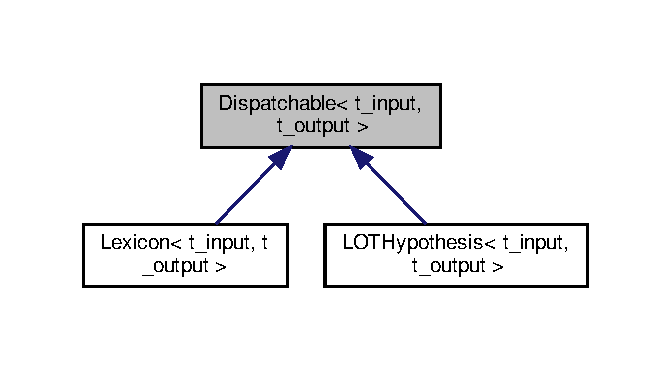
\includegraphics[width=322pt]{class_dispatchable__inherit__graph}
\end{center}
\end{figure}
\subsection*{Public Member Functions}
\begin{DoxyCompactItemize}
\item 
virtual \hyperlink{_instruction_8h_a6202215407ab29590bb936ca2996cf64}{vmstatus\+\_\+t} \hyperlink{class_dispatchable_a6d2bd844b0e55378d29ed85e718d0a77}{dispatch\+\_\+custom} (\hyperlink{class_instruction}{Instruction} i, \hyperlink{class_virtual_machine_pool}{Virtual\+Machine\+Pool}$<$ t\+\_\+input, t\+\_\+output $>$ $\ast$pool, \hyperlink{class_virtual_machine_state}{Virtual\+Machine\+State}$<$ t\+\_\+input, t\+\_\+output $>$ $\ast$vms, \hyperlink{class_dispatchable}{Dispatchable}$<$ t\+\_\+input, t\+\_\+output $>$ $\ast$loader)=0
\item 
virtual void \hyperlink{class_dispatchable_a9339c2906f7c8dadbe1d0ca79dd9bb11}{push\+\_\+program} (Program \&, short)=0
\end{DoxyCompactItemize}


\subsection{Detailed Description}
\subsubsection*{template$<$typename t\+\_\+input, typename t\+\_\+output$>$\newline
class Dispatchable$<$ t\+\_\+input, t\+\_\+output $>$}

\begin{DoxyAuthor}{Author}
steven piantadosi 
\end{DoxyAuthor}
\begin{DoxyDate}{Date}
03/02/20 
\end{DoxyDate}


\subsection{Member Function Documentation}
\mbox{\Hypertarget{class_dispatchable_a6d2bd844b0e55378d29ed85e718d0a77}\label{class_dispatchable_a6d2bd844b0e55378d29ed85e718d0a77}} 
\index{Dispatchable@{Dispatchable}!dispatch\+\_\+custom@{dispatch\+\_\+custom}}
\index{dispatch\+\_\+custom@{dispatch\+\_\+custom}!Dispatchable@{Dispatchable}}
\subsubsection{\texorpdfstring{dispatch\+\_\+custom()}{dispatch\_custom()}}
{\footnotesize\ttfamily template$<$typename t\+\_\+input, typename t\+\_\+output$>$ \\
virtual \hyperlink{_instruction_8h_a6202215407ab29590bb936ca2996cf64}{vmstatus\+\_\+t} \hyperlink{class_dispatchable}{Dispatchable}$<$ t\+\_\+input, t\+\_\+output $>$\+::dispatch\+\_\+custom (\begin{DoxyParamCaption}\item[{\hyperlink{class_instruction}{Instruction}}]{i,  }\item[{\hyperlink{class_virtual_machine_pool}{Virtual\+Machine\+Pool}$<$ t\+\_\+input, t\+\_\+output $>$ $\ast$}]{pool,  }\item[{\hyperlink{class_virtual_machine_state}{Virtual\+Machine\+State}$<$ t\+\_\+input, t\+\_\+output $>$ $\ast$}]{vms,  }\item[{\hyperlink{class_dispatchable}{Dispatchable}$<$ t\+\_\+input, t\+\_\+output $>$ $\ast$}]{loader }\end{DoxyParamCaption})\hspace{0.3cm}{\ttfamily [pure virtual]}}



Implemented in \hyperlink{class_lexicon_a1c6b61ac505114f23441e3097163685b}{Lexicon$<$ H\+Y\+P, T, t\+\_\+input, t\+\_\+output, t\+\_\+datum $>$}, \hyperlink{class_lexicon_a1c6b61ac505114f23441e3097163685b}{Lexicon$<$ My\+Hypothesis, Inner\+Hypothesis, S, S $>$}, \hyperlink{class_inner_hypothesis_a9aea852725a3798aafeae5e7a5a0736b}{Inner\+Hypothesis}, \hyperlink{class_l_o_t_hypothesis_a6eae1ce4486971909e0245ab9e30ddeb}{L\+O\+T\+Hypothesis$<$ H\+Y\+P, T, t\+\_\+input, t\+\_\+output, \+\_\+t\+\_\+datum, \+\_\+t\+\_\+data $>$}, \hyperlink{class_l_o_t_hypothesis_a6eae1ce4486971909e0245ab9e30ddeb}{L\+O\+T\+Hypothesis$<$ Inner\+Hypothesis, Node, S, S $>$}, \hyperlink{class_l_o_t_hypothesis_a6eae1ce4486971909e0245ab9e30ddeb}{L\+O\+T\+Hypothesis$<$ My\+Hypothesis, Node, Object, bool $>$}, \hyperlink{class_l_o_t_hypothesis_a6eae1ce4486971909e0245ab9e30ddeb}{L\+O\+T\+Hypothesis$<$ My\+Hypothesis, Node, float, float, float, std\+::multiset$<$ float $>$ $>$}, and \hyperlink{class_my_hypothesis_a3de47a545e8824bb8c63181965c62a01}{My\+Hypothesis}.

\mbox{\Hypertarget{class_dispatchable_a9339c2906f7c8dadbe1d0ca79dd9bb11}\label{class_dispatchable_a9339c2906f7c8dadbe1d0ca79dd9bb11}} 
\index{Dispatchable@{Dispatchable}!push\+\_\+program@{push\+\_\+program}}
\index{push\+\_\+program@{push\+\_\+program}!Dispatchable@{Dispatchable}}
\subsubsection{\texorpdfstring{push\+\_\+program()}{push\_program()}}
{\footnotesize\ttfamily template$<$typename t\+\_\+input, typename t\+\_\+output$>$ \\
virtual void \hyperlink{class_dispatchable}{Dispatchable}$<$ t\+\_\+input, t\+\_\+output $>$\+::push\+\_\+program (\begin{DoxyParamCaption}\item[{Program \&}]{,  }\item[{short}]{ }\end{DoxyParamCaption})\hspace{0.3cm}{\ttfamily [pure virtual]}}



Implemented in \hyperlink{class_lexicon_af85ffc6944b66e92f760aaf7e3521d23}{Lexicon$<$ H\+Y\+P, T, t\+\_\+input, t\+\_\+output, t\+\_\+datum $>$}, \hyperlink{class_lexicon_af85ffc6944b66e92f760aaf7e3521d23}{Lexicon$<$ My\+Hypothesis, Inner\+Hypothesis, S, S $>$}, \hyperlink{class_l_o_t_hypothesis_a0c0048d364936ae2a1bbeeca08959215}{L\+O\+T\+Hypothesis$<$ H\+Y\+P, T, t\+\_\+input, t\+\_\+output, \+\_\+t\+\_\+datum, \+\_\+t\+\_\+data $>$}, \hyperlink{class_l_o_t_hypothesis_a0c0048d364936ae2a1bbeeca08959215}{L\+O\+T\+Hypothesis$<$ Inner\+Hypothesis, Node, S, S $>$}, \hyperlink{class_l_o_t_hypothesis_a0c0048d364936ae2a1bbeeca08959215}{L\+O\+T\+Hypothesis$<$ My\+Hypothesis, Node, Object, bool $>$}, and \hyperlink{class_l_o_t_hypothesis_a0c0048d364936ae2a1bbeeca08959215}{L\+O\+T\+Hypothesis$<$ My\+Hypothesis, Node, float, float, float, std\+::multiset$<$ float $>$ $>$}.



The documentation for this class was generated from the following file\+:\begin{DoxyCompactItemize}
\item 
src/\+Hypotheses/\+Interfaces/\hyperlink{_dispatchable_8h}{Dispatchable.\+h}\end{DoxyCompactItemize}

\hypertarget{class_fleet_1_1_statistics_1_1_finite_history}{}\section{Fleet\+:\+:Statistics\+:\+:Finite\+History$<$ T $>$ Class Template Reference}
\label{class_fleet_1_1_statistics_1_1_finite_history}\index{Fleet\+::\+Statistics\+::\+Finite\+History$<$ T $>$@{Fleet\+::\+Statistics\+::\+Finite\+History$<$ T $>$}}


{\ttfamily \#include $<$Finite\+History.\+h$>$}

\subsection*{Public Member Functions}
\begin{DoxyCompactItemize}
\item 
\hyperlink{class_fleet_1_1_statistics_1_1_finite_history_a14ef23d9161c620fa8dce3c42ce08220}{Finite\+History} (size\+\_\+t n)
\item 
\hyperlink{class_fleet_1_1_statistics_1_1_finite_history_ae4ca3e409992b855cef8e9430a216481}{Finite\+History} ()
\item 
\hyperlink{class_fleet_1_1_statistics_1_1_finite_history_a7c94246e763c8f3533a5aeecb3d74997}{Finite\+History} (const \hyperlink{class_fleet_1_1_statistics_1_1_finite_history}{Finite\+History} \&fh)
\item 
\hyperlink{class_fleet_1_1_statistics_1_1_finite_history_a60518d678c82115b004bbc8c319e8a63}{Finite\+History} (\hyperlink{class_fleet_1_1_statistics_1_1_finite_history}{Finite\+History} \&\&fh)
\item 
void \hyperlink{class_fleet_1_1_statistics_1_1_finite_history_a68f88a68354e3e420ca350eb6afb94cc}{operator=} (const \hyperlink{class_fleet_1_1_statistics_1_1_finite_history}{Finite\+History} \&fh)
\item 
void \hyperlink{class_fleet_1_1_statistics_1_1_finite_history_a70d3185c2d7a2a00e92cc2680d5db027}{operator=} (\hyperlink{class_fleet_1_1_statistics_1_1_finite_history}{Finite\+History} \&\&fh)
\item 
void \hyperlink{class_fleet_1_1_statistics_1_1_finite_history_a00fd21941d00d71818d6a83c2c7160e5}{add} (T x)
\begin{DoxyCompactList}\small\item\em Add x to this history. \end{DoxyCompactList}\item 
void \hyperlink{class_fleet_1_1_statistics_1_1_finite_history_acee6a049c14cb100dca992444b84d9ec}{operator$<$$<$} (T x)
\begin{DoxyCompactList}\small\item\em Convenient adding. \end{DoxyCompactList}\item 
double \hyperlink{class_fleet_1_1_statistics_1_1_finite_history_a7ece3121889428a4082fbe88fdacc106}{mean} ()
\begin{DoxyCompactList}\small\item\em Compute the average. \end{DoxyCompactList}\end{DoxyCompactItemize}
\subsection*{Public Attributes}
\begin{DoxyCompactItemize}
\item 
std\+::vector$<$ T $>$ \hyperlink{class_fleet_1_1_statistics_1_1_finite_history_a567aa8bf1cbbb762b82b6910e5cd92cd}{history}
\item 
std\+::atomic$<$ size\+\_\+t $>$ \hyperlink{class_fleet_1_1_statistics_1_1_finite_history_a5ed75416ad7a32def48ee647918e5734}{history\+\_\+size}
\item 
std\+::atomic$<$ size\+\_\+t $>$ \hyperlink{class_fleet_1_1_statistics_1_1_finite_history_a05063bf9616d2b49fc35f10a2d071552}{history\+\_\+index}
\item 
std\+::atomic$<$ unsigned long $>$ \hyperlink{class_fleet_1_1_statistics_1_1_finite_history_a67d34a239140f65d8ca07de2a10c45c9}{N}
\item 
std\+::mutex \hyperlink{class_fleet_1_1_statistics_1_1_finite_history_abae96d2bf212abbf0bcfb74ac41b7165}{mutex}
\end{DoxyCompactItemize}


\subsection{Detailed Description}
\subsubsection*{template$<$typename T$>$\newline
class Fleet\+::\+Statistics\+::\+Finite\+History$<$ T $>$}

\begin{DoxyAuthor}{Author}
steven piantadosi 
\end{DoxyAuthor}
\begin{DoxyDate}{Date}
03/02/20 
\end{DoxyDate}


\subsection{Constructor \& Destructor Documentation}
\mbox{\Hypertarget{class_fleet_1_1_statistics_1_1_finite_history_a14ef23d9161c620fa8dce3c42ce08220}\label{class_fleet_1_1_statistics_1_1_finite_history_a14ef23d9161c620fa8dce3c42ce08220}} 
\index{Fleet\+::\+Statistics\+::\+Finite\+History@{Fleet\+::\+Statistics\+::\+Finite\+History}!Finite\+History@{Finite\+History}}
\index{Finite\+History@{Finite\+History}!Fleet\+::\+Statistics\+::\+Finite\+History@{Fleet\+::\+Statistics\+::\+Finite\+History}}
\subsubsection{\texorpdfstring{Finite\+History()}{FiniteHistory()}\hspace{0.1cm}{\footnotesize\ttfamily [1/4]}}
{\footnotesize\ttfamily template$<$typename T$>$ \\
\hyperlink{class_fleet_1_1_statistics_1_1_finite_history}{Fleet\+::\+Statistics\+::\+Finite\+History}$<$ T $>$\+::\hyperlink{class_fleet_1_1_statistics_1_1_finite_history}{Finite\+History} (\begin{DoxyParamCaption}\item[{size\+\_\+t}]{n }\end{DoxyParamCaption})\hspace{0.3cm}{\ttfamily [inline]}}

\mbox{\Hypertarget{class_fleet_1_1_statistics_1_1_finite_history_ae4ca3e409992b855cef8e9430a216481}\label{class_fleet_1_1_statistics_1_1_finite_history_ae4ca3e409992b855cef8e9430a216481}} 
\index{Fleet\+::\+Statistics\+::\+Finite\+History@{Fleet\+::\+Statistics\+::\+Finite\+History}!Finite\+History@{Finite\+History}}
\index{Finite\+History@{Finite\+History}!Fleet\+::\+Statistics\+::\+Finite\+History@{Fleet\+::\+Statistics\+::\+Finite\+History}}
\subsubsection{\texorpdfstring{Finite\+History()}{FiniteHistory()}\hspace{0.1cm}{\footnotesize\ttfamily [2/4]}}
{\footnotesize\ttfamily template$<$typename T$>$ \\
\hyperlink{class_fleet_1_1_statistics_1_1_finite_history}{Fleet\+::\+Statistics\+::\+Finite\+History}$<$ T $>$\+::\hyperlink{class_fleet_1_1_statistics_1_1_finite_history}{Finite\+History} (\begin{DoxyParamCaption}{ }\end{DoxyParamCaption})\hspace{0.3cm}{\ttfamily [inline]}}

\mbox{\Hypertarget{class_fleet_1_1_statistics_1_1_finite_history_a7c94246e763c8f3533a5aeecb3d74997}\label{class_fleet_1_1_statistics_1_1_finite_history_a7c94246e763c8f3533a5aeecb3d74997}} 
\index{Fleet\+::\+Statistics\+::\+Finite\+History@{Fleet\+::\+Statistics\+::\+Finite\+History}!Finite\+History@{Finite\+History}}
\index{Finite\+History@{Finite\+History}!Fleet\+::\+Statistics\+::\+Finite\+History@{Fleet\+::\+Statistics\+::\+Finite\+History}}
\subsubsection{\texorpdfstring{Finite\+History()}{FiniteHistory()}\hspace{0.1cm}{\footnotesize\ttfamily [3/4]}}
{\footnotesize\ttfamily template$<$typename T$>$ \\
\hyperlink{class_fleet_1_1_statistics_1_1_finite_history}{Fleet\+::\+Statistics\+::\+Finite\+History}$<$ T $>$\+::\hyperlink{class_fleet_1_1_statistics_1_1_finite_history}{Finite\+History} (\begin{DoxyParamCaption}\item[{const \hyperlink{class_fleet_1_1_statistics_1_1_finite_history}{Finite\+History}$<$ T $>$ \&}]{fh }\end{DoxyParamCaption})\hspace{0.3cm}{\ttfamily [inline]}}

\mbox{\Hypertarget{class_fleet_1_1_statistics_1_1_finite_history_a60518d678c82115b004bbc8c319e8a63}\label{class_fleet_1_1_statistics_1_1_finite_history_a60518d678c82115b004bbc8c319e8a63}} 
\index{Fleet\+::\+Statistics\+::\+Finite\+History@{Fleet\+::\+Statistics\+::\+Finite\+History}!Finite\+History@{Finite\+History}}
\index{Finite\+History@{Finite\+History}!Fleet\+::\+Statistics\+::\+Finite\+History@{Fleet\+::\+Statistics\+::\+Finite\+History}}
\subsubsection{\texorpdfstring{Finite\+History()}{FiniteHistory()}\hspace{0.1cm}{\footnotesize\ttfamily [4/4]}}
{\footnotesize\ttfamily template$<$typename T$>$ \\
\hyperlink{class_fleet_1_1_statistics_1_1_finite_history}{Fleet\+::\+Statistics\+::\+Finite\+History}$<$ T $>$\+::\hyperlink{class_fleet_1_1_statistics_1_1_finite_history}{Finite\+History} (\begin{DoxyParamCaption}\item[{\hyperlink{class_fleet_1_1_statistics_1_1_finite_history}{Finite\+History}$<$ T $>$ \&\&}]{fh }\end{DoxyParamCaption})\hspace{0.3cm}{\ttfamily [inline]}}



\subsection{Member Function Documentation}
\mbox{\Hypertarget{class_fleet_1_1_statistics_1_1_finite_history_a00fd21941d00d71818d6a83c2c7160e5}\label{class_fleet_1_1_statistics_1_1_finite_history_a00fd21941d00d71818d6a83c2c7160e5}} 
\index{Fleet\+::\+Statistics\+::\+Finite\+History@{Fleet\+::\+Statistics\+::\+Finite\+History}!add@{add}}
\index{add@{add}!Fleet\+::\+Statistics\+::\+Finite\+History@{Fleet\+::\+Statistics\+::\+Finite\+History}}
\subsubsection{\texorpdfstring{add()}{add()}}
{\footnotesize\ttfamily template$<$typename T$>$ \\
void \hyperlink{class_fleet_1_1_statistics_1_1_finite_history}{Fleet\+::\+Statistics\+::\+Finite\+History}$<$ T $>$\+::add (\begin{DoxyParamCaption}\item[{T}]{x }\end{DoxyParamCaption})\hspace{0.3cm}{\ttfamily [inline]}}



Add x to this history. 


\begin{DoxyParams}{Parameters}
{\em x} & \\
\hline
\end{DoxyParams}
\mbox{\Hypertarget{class_fleet_1_1_statistics_1_1_finite_history_a7ece3121889428a4082fbe88fdacc106}\label{class_fleet_1_1_statistics_1_1_finite_history_a7ece3121889428a4082fbe88fdacc106}} 
\index{Fleet\+::\+Statistics\+::\+Finite\+History@{Fleet\+::\+Statistics\+::\+Finite\+History}!mean@{mean}}
\index{mean@{mean}!Fleet\+::\+Statistics\+::\+Finite\+History@{Fleet\+::\+Statistics\+::\+Finite\+History}}
\subsubsection{\texorpdfstring{mean()}{mean()}}
{\footnotesize\ttfamily template$<$typename T$>$ \\
double \hyperlink{class_fleet_1_1_statistics_1_1_finite_history}{Fleet\+::\+Statistics\+::\+Finite\+History}$<$ T $>$\+::mean (\begin{DoxyParamCaption}{ }\end{DoxyParamCaption})\hspace{0.3cm}{\ttfamily [inline]}}



Compute the average. 

\begin{DoxyReturn}{Returns}

\end{DoxyReturn}
\mbox{\Hypertarget{class_fleet_1_1_statistics_1_1_finite_history_acee6a049c14cb100dca992444b84d9ec}\label{class_fleet_1_1_statistics_1_1_finite_history_acee6a049c14cb100dca992444b84d9ec}} 
\index{Fleet\+::\+Statistics\+::\+Finite\+History@{Fleet\+::\+Statistics\+::\+Finite\+History}!operator$<$$<$@{operator$<$$<$}}
\index{operator$<$$<$@{operator$<$$<$}!Fleet\+::\+Statistics\+::\+Finite\+History@{Fleet\+::\+Statistics\+::\+Finite\+History}}
\subsubsection{\texorpdfstring{operator$<$$<$()}{operator<<()}}
{\footnotesize\ttfamily template$<$typename T$>$ \\
void \hyperlink{class_fleet_1_1_statistics_1_1_finite_history}{Fleet\+::\+Statistics\+::\+Finite\+History}$<$ T $>$\+::operator$<$$<$ (\begin{DoxyParamCaption}\item[{T}]{x }\end{DoxyParamCaption})\hspace{0.3cm}{\ttfamily [inline]}}



Convenient adding. 


\begin{DoxyParams}{Parameters}
{\em x} & \\
\hline
\end{DoxyParams}
\mbox{\Hypertarget{class_fleet_1_1_statistics_1_1_finite_history_a68f88a68354e3e420ca350eb6afb94cc}\label{class_fleet_1_1_statistics_1_1_finite_history_a68f88a68354e3e420ca350eb6afb94cc}} 
\index{Fleet\+::\+Statistics\+::\+Finite\+History@{Fleet\+::\+Statistics\+::\+Finite\+History}!operator=@{operator=}}
\index{operator=@{operator=}!Fleet\+::\+Statistics\+::\+Finite\+History@{Fleet\+::\+Statistics\+::\+Finite\+History}}
\subsubsection{\texorpdfstring{operator=()}{operator=()}\hspace{0.1cm}{\footnotesize\ttfamily [1/2]}}
{\footnotesize\ttfamily template$<$typename T$>$ \\
void \hyperlink{class_fleet_1_1_statistics_1_1_finite_history}{Fleet\+::\+Statistics\+::\+Finite\+History}$<$ T $>$\+::operator= (\begin{DoxyParamCaption}\item[{const \hyperlink{class_fleet_1_1_statistics_1_1_finite_history}{Finite\+History}$<$ T $>$ \&}]{fh }\end{DoxyParamCaption})\hspace{0.3cm}{\ttfamily [inline]}}

\mbox{\Hypertarget{class_fleet_1_1_statistics_1_1_finite_history_a70d3185c2d7a2a00e92cc2680d5db027}\label{class_fleet_1_1_statistics_1_1_finite_history_a70d3185c2d7a2a00e92cc2680d5db027}} 
\index{Fleet\+::\+Statistics\+::\+Finite\+History@{Fleet\+::\+Statistics\+::\+Finite\+History}!operator=@{operator=}}
\index{operator=@{operator=}!Fleet\+::\+Statistics\+::\+Finite\+History@{Fleet\+::\+Statistics\+::\+Finite\+History}}
\subsubsection{\texorpdfstring{operator=()}{operator=()}\hspace{0.1cm}{\footnotesize\ttfamily [2/2]}}
{\footnotesize\ttfamily template$<$typename T$>$ \\
void \hyperlink{class_fleet_1_1_statistics_1_1_finite_history}{Fleet\+::\+Statistics\+::\+Finite\+History}$<$ T $>$\+::operator= (\begin{DoxyParamCaption}\item[{\hyperlink{class_fleet_1_1_statistics_1_1_finite_history}{Finite\+History}$<$ T $>$ \&\&}]{fh }\end{DoxyParamCaption})\hspace{0.3cm}{\ttfamily [inline]}}



\subsection{Member Data Documentation}
\mbox{\Hypertarget{class_fleet_1_1_statistics_1_1_finite_history_a567aa8bf1cbbb762b82b6910e5cd92cd}\label{class_fleet_1_1_statistics_1_1_finite_history_a567aa8bf1cbbb762b82b6910e5cd92cd}} 
\index{Fleet\+::\+Statistics\+::\+Finite\+History@{Fleet\+::\+Statistics\+::\+Finite\+History}!history@{history}}
\index{history@{history}!Fleet\+::\+Statistics\+::\+Finite\+History@{Fleet\+::\+Statistics\+::\+Finite\+History}}
\subsubsection{\texorpdfstring{history}{history}}
{\footnotesize\ttfamily template$<$typename T$>$ \\
std\+::vector$<$T$>$ \hyperlink{class_fleet_1_1_statistics_1_1_finite_history}{Fleet\+::\+Statistics\+::\+Finite\+History}$<$ T $>$\+::history}

\mbox{\Hypertarget{class_fleet_1_1_statistics_1_1_finite_history_a05063bf9616d2b49fc35f10a2d071552}\label{class_fleet_1_1_statistics_1_1_finite_history_a05063bf9616d2b49fc35f10a2d071552}} 
\index{Fleet\+::\+Statistics\+::\+Finite\+History@{Fleet\+::\+Statistics\+::\+Finite\+History}!history\+\_\+index@{history\+\_\+index}}
\index{history\+\_\+index@{history\+\_\+index}!Fleet\+::\+Statistics\+::\+Finite\+History@{Fleet\+::\+Statistics\+::\+Finite\+History}}
\subsubsection{\texorpdfstring{history\+\_\+index}{history\_index}}
{\footnotesize\ttfamily template$<$typename T$>$ \\
std\+::atomic$<$size\+\_\+t$>$ \hyperlink{class_fleet_1_1_statistics_1_1_finite_history}{Fleet\+::\+Statistics\+::\+Finite\+History}$<$ T $>$\+::history\+\_\+index}

\mbox{\Hypertarget{class_fleet_1_1_statistics_1_1_finite_history_a5ed75416ad7a32def48ee647918e5734}\label{class_fleet_1_1_statistics_1_1_finite_history_a5ed75416ad7a32def48ee647918e5734}} 
\index{Fleet\+::\+Statistics\+::\+Finite\+History@{Fleet\+::\+Statistics\+::\+Finite\+History}!history\+\_\+size@{history\+\_\+size}}
\index{history\+\_\+size@{history\+\_\+size}!Fleet\+::\+Statistics\+::\+Finite\+History@{Fleet\+::\+Statistics\+::\+Finite\+History}}
\subsubsection{\texorpdfstring{history\+\_\+size}{history\_size}}
{\footnotesize\ttfamily template$<$typename T$>$ \\
std\+::atomic$<$size\+\_\+t$>$ \hyperlink{class_fleet_1_1_statistics_1_1_finite_history}{Fleet\+::\+Statistics\+::\+Finite\+History}$<$ T $>$\+::history\+\_\+size}

\mbox{\Hypertarget{class_fleet_1_1_statistics_1_1_finite_history_abae96d2bf212abbf0bcfb74ac41b7165}\label{class_fleet_1_1_statistics_1_1_finite_history_abae96d2bf212abbf0bcfb74ac41b7165}} 
\index{Fleet\+::\+Statistics\+::\+Finite\+History@{Fleet\+::\+Statistics\+::\+Finite\+History}!mutex@{mutex}}
\index{mutex@{mutex}!Fleet\+::\+Statistics\+::\+Finite\+History@{Fleet\+::\+Statistics\+::\+Finite\+History}}
\subsubsection{\texorpdfstring{mutex}{mutex}}
{\footnotesize\ttfamily template$<$typename T$>$ \\
std\+::mutex \hyperlink{class_fleet_1_1_statistics_1_1_finite_history}{Fleet\+::\+Statistics\+::\+Finite\+History}$<$ T $>$\+::mutex\hspace{0.3cm}{\ttfamily [mutable]}}

\mbox{\Hypertarget{class_fleet_1_1_statistics_1_1_finite_history_a67d34a239140f65d8ca07de2a10c45c9}\label{class_fleet_1_1_statistics_1_1_finite_history_a67d34a239140f65d8ca07de2a10c45c9}} 
\index{Fleet\+::\+Statistics\+::\+Finite\+History@{Fleet\+::\+Statistics\+::\+Finite\+History}!N@{N}}
\index{N@{N}!Fleet\+::\+Statistics\+::\+Finite\+History@{Fleet\+::\+Statistics\+::\+Finite\+History}}
\subsubsection{\texorpdfstring{N}{N}}
{\footnotesize\ttfamily template$<$typename T$>$ \\
std\+::atomic$<$unsigned long$>$ \hyperlink{class_fleet_1_1_statistics_1_1_finite_history}{Fleet\+::\+Statistics\+::\+Finite\+History}$<$ T $>$\+::N}



The documentation for this class was generated from the following file\+:\begin{DoxyCompactItemize}
\item 
src/\+Statistics/\hyperlink{_finite_history_8h}{Finite\+History.\+h}\end{DoxyCompactItemize}

\hypertarget{struct_builtin_1_1_flip}{}\section{Builtin\+:\+:Flip Struct Reference}
\label{struct_builtin_1_1_flip}\index{Builtin\+::\+Flip@{Builtin\+::\+Flip}}


{\ttfamily \#include $<$Builtins.\+h$>$}



Inheritance diagram for Builtin\+:\+:Flip\+:\nopagebreak
\begin{figure}[H]
\begin{center}
\leavevmode
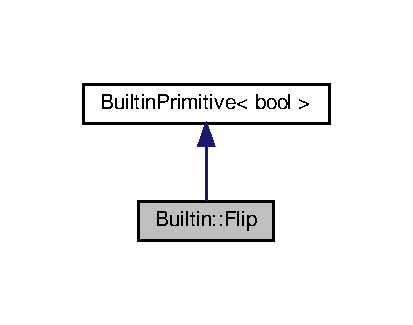
\includegraphics[width=198pt]{struct_builtin_1_1_flip__inherit__graph}
\end{center}
\end{figure}


Collaboration diagram for Builtin\+:\+:Flip\+:\nopagebreak
\begin{figure}[H]
\begin{center}
\leavevmode
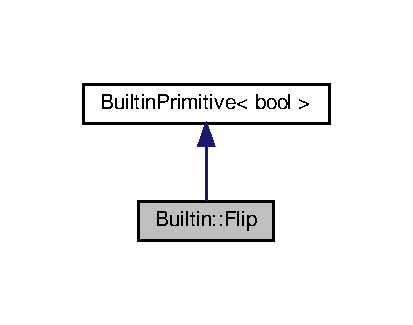
\includegraphics[width=198pt]{struct_builtin_1_1_flip__coll__graph}
\end{center}
\end{figure}
\subsection*{Public Member Functions}
\begin{DoxyCompactItemize}
\item 
\hyperlink{struct_builtin_1_1_flip_a7b2664f6342725c1f1fb91d770b34843}{Flip} (std\+::string fmt, double \+\_\+p=1.\+0)
\end{DoxyCompactItemize}
\subsection*{Additional Inherited Members}


\subsection{Constructor \& Destructor Documentation}
\mbox{\Hypertarget{struct_builtin_1_1_flip_a7b2664f6342725c1f1fb91d770b34843}\label{struct_builtin_1_1_flip_a7b2664f6342725c1f1fb91d770b34843}} 
\index{Builtin\+::\+Flip@{Builtin\+::\+Flip}!Flip@{Flip}}
\index{Flip@{Flip}!Builtin\+::\+Flip@{Builtin\+::\+Flip}}
\subsubsection{\texorpdfstring{Flip()}{Flip()}}
{\footnotesize\ttfamily Builtin\+::\+Flip\+::\+Flip (\begin{DoxyParamCaption}\item[{std\+::string}]{fmt,  }\item[{double}]{\+\_\+p = {\ttfamily 1.0} }\end{DoxyParamCaption})\hspace{0.3cm}{\ttfamily [inline]}}



The documentation for this struct was generated from the following file\+:\begin{DoxyCompactItemize}
\item 
src/\+Virtual\+Machine/\hyperlink{_builtins_8h}{Builtins.\+h}\end{DoxyCompactItemize}

\hypertarget{struct_builtin_1_1_flip_p}{}\section{Builtin\+:\+:FlipP Struct Reference}
\label{struct_builtin_1_1_flip_p}\index{Builtin\+::\+FlipP@{Builtin\+::\+FlipP}}


{\ttfamily \#include $<$Builtins.\+h$>$}



Inheritance diagram for Builtin\+:\+:FlipP\+:\nopagebreak
\begin{figure}[H]
\begin{center}
\leavevmode
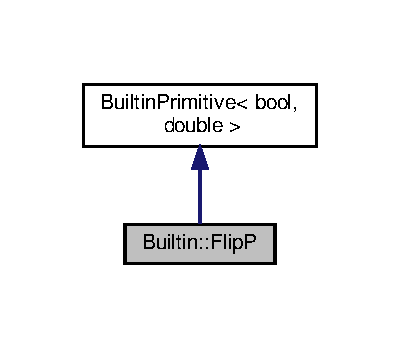
\includegraphics[width=192pt]{struct_builtin_1_1_flip_p__inherit__graph}
\end{center}
\end{figure}


Collaboration diagram for Builtin\+:\+:FlipP\+:\nopagebreak
\begin{figure}[H]
\begin{center}
\leavevmode
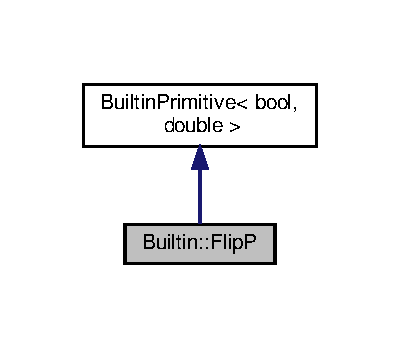
\includegraphics[width=192pt]{struct_builtin_1_1_flip_p__coll__graph}
\end{center}
\end{figure}
\subsection*{Public Member Functions}
\begin{DoxyCompactItemize}
\item 
\hyperlink{struct_builtin_1_1_flip_p_adab32b985984688bb906fef95301c7fa}{FlipP} (std\+::string fmt, double \+\_\+p=1.\+0)
\end{DoxyCompactItemize}
\subsection*{Additional Inherited Members}


\subsection{Constructor \& Destructor Documentation}
\mbox{\Hypertarget{struct_builtin_1_1_flip_p_adab32b985984688bb906fef95301c7fa}\label{struct_builtin_1_1_flip_p_adab32b985984688bb906fef95301c7fa}} 
\index{Builtin\+::\+FlipP@{Builtin\+::\+FlipP}!FlipP@{FlipP}}
\index{FlipP@{FlipP}!Builtin\+::\+FlipP@{Builtin\+::\+FlipP}}
\subsubsection{\texorpdfstring{Flip\+P()}{FlipP()}}
{\footnotesize\ttfamily Builtin\+::\+Flip\+P\+::\+FlipP (\begin{DoxyParamCaption}\item[{std\+::string}]{fmt,  }\item[{double}]{\+\_\+p = {\ttfamily 1.0} }\end{DoxyParamCaption})\hspace{0.3cm}{\ttfamily [inline]}}



The documentation for this struct was generated from the following file\+:\begin{DoxyCompactItemize}
\item 
src/\+Virtual\+Machine/\hyperlink{_builtins_8h}{Builtins.\+h}\end{DoxyCompactItemize}

\hypertarget{class_grammar}{}\section{Grammar Class Reference}
\label{class_grammar}\index{Grammar@{Grammar}}


{\ttfamily \#include $<$Grammar.\+h$>$}

\subsection*{Public Member Functions}
\begin{DoxyCompactItemize}
\item 
{\footnotesize template$<$class T $>$ }\\constexpr nonterminal\+\_\+t \hyperlink{class_grammar_aa5c9afa0e7e1aa989b54402b02a677a3}{nt} ()
\item 
\hyperlink{class_grammar_aa201250a002a7d07d398fee189a74427}{Grammar} ()
\item 
{\footnotesize template$<$typename... T$>$ }\\\hyperlink{class_grammar_a4e0a3b86d64eba75726b7355308c4649}{Grammar} (std\+::tuple$<$ T... $>$ tup)
\item 
\hyperlink{class_grammar_acfb7e4ea64210d03de896e300447e760}{Grammar} (const \hyperlink{class_grammar}{Grammar} \&g)=delete
\item 
\hyperlink{class_grammar_a28f97335602afe8b1a612679de2f80d9}{Grammar} (const \hyperlink{class_grammar}{Grammar} \&\&g)=delete
\item 
size\+\_\+t \hyperlink{class_grammar_abf841bc64ac19cb9872a8362f5e5731a}{count\+\_\+nonterminals} () const
\item 
size\+\_\+t \hyperlink{class_grammar_af25c47a2c5cae2a11720c8454e59290f}{count\+\_\+rules} (const nonterminal\+\_\+t \hyperlink{class_grammar_aa5c9afa0e7e1aa989b54402b02a677a3}{nt}) const
\item 
size\+\_\+t \hyperlink{class_grammar_af8f0fdd9cb368a608bee5626774360d4}{count\+\_\+rules} () const
\item 
size\+\_\+t \hyperlink{class_grammar_a7cf0515f3ca761590da05455a417896b}{count\+\_\+terminals} (nonterminal\+\_\+t \hyperlink{class_grammar_aa5c9afa0e7e1aa989b54402b02a677a3}{nt}) const
\item 
size\+\_\+t \hyperlink{class_grammar_a0714d68070749932d876fe868bde94bd}{count\+\_\+nonterminals} (nonterminal\+\_\+t \hyperlink{class_grammar_aa5c9afa0e7e1aa989b54402b02a677a3}{nt}) const
\item 
size\+\_\+t \hyperlink{class_grammar_a9c015fe6f16191ddb2f21a51f1931a05}{count\+\_\+expansions} (const nonterminal\+\_\+t \hyperlink{class_grammar_aa5c9afa0e7e1aa989b54402b02a677a3}{nt}) const
\item 
void \hyperlink{class_grammar_aa3c730ea64c8ca5d93fecb4275f2e380}{show} (std\+::string prefix=\char`\"{}\# \char`\"{})
\item 
virtual void \hyperlink{class_grammar_af0b97cbaf14fc6be7495c8bb9e888002}{add} (\hyperlink{class_rule}{Rule} \&\&r)
\item 
{\footnotesize template$<$typename... args, size\+\_\+t... Is$>$ }\\void \hyperlink{class_grammar_a37a1dd90b7a315fe97bbdefad7c09df9}{add} (std\+::tuple$<$ args... $>$ t, std\+::index\+\_\+sequence$<$ Is... $>$)
\item 
{\footnotesize template$<$typename T , typename... args$>$ }\\void \hyperlink{class_grammar_a0af8f369b948cde8ee5d403311ec8fa9}{add} (\hyperlink{struct_primitive}{Primitive}$<$ T, args... $>$ p, const int arg=0)
\item 
{\footnotesize template$<$typename T , typename... args$>$ }\\void \hyperlink{class_grammar_af96467de4413d3e5a0d2f291992365d9}{add} (\hyperlink{struct_builtin_primitive}{Builtin\+Primitive}$<$ T, args... $>$ p, const int arg=0)
\item 
{\footnotesize template$<$typename T , typename... args$>$ }\\void \hyperlink{class_grammar_a562f3b4113e3f2764832ac828ffb58fc}{add} (\hyperlink{_instruction_8h_af2fb7c87c5854c5733d7bb0506b06de7}{Builtin\+Op} o, std\+::string format, const double p=1.\+0, const int arg=0)
\item 
{\footnotesize template$<$typename T , typename... args$>$ }\\void \hyperlink{class_grammar_aba61b4a7563c249a27ad7b6b808ee575}{add} (\hyperlink{_instruction_8h_a3a20ca4a8f0ab220518b030cc23ffee4}{Custom\+Op} o, std\+::string format, const double p=1.\+0, const int arg=0)
\item 
size\+\_\+t \hyperlink{class_grammar_affec19f6e91201c8d29119bf50ffa3e6}{get\+\_\+index\+\_\+of} (const \hyperlink{class_rule}{Rule} $\ast$r) const
\item 
virtual \hyperlink{class_rule}{Rule} $\ast$ \hyperlink{class_grammar_aea24b7ae4a2d61f322504a9f49478bb4}{get\+\_\+rule} (const nonterminal\+\_\+t \hyperlink{class_grammar_aa5c9afa0e7e1aa989b54402b02a677a3}{nt}, size\+\_\+t k) const
\item 
virtual \hyperlink{class_rule}{Rule} $\ast$ \hyperlink{class_grammar_aa642e370571830772b8d3be70cb5a5c7}{get\+\_\+rule} (const nonterminal\+\_\+t \hyperlink{class_grammar_aa5c9afa0e7e1aa989b54402b02a677a3}{nt}, const \hyperlink{_instruction_8h_a3a20ca4a8f0ab220518b030cc23ffee4}{Custom\+Op} o, const int a=0)
\item 
virtual \hyperlink{class_rule}{Rule} $\ast$ \hyperlink{class_grammar_ab82ed6614e4fcced4d0e7c742e1c5e4b}{get\+\_\+rule} (const nonterminal\+\_\+t \hyperlink{class_grammar_aa5c9afa0e7e1aa989b54402b02a677a3}{nt}, const \hyperlink{_instruction_8h_af2fb7c87c5854c5733d7bb0506b06de7}{Builtin\+Op} o, const int a=0)
\item 
virtual \hyperlink{class_rule}{Rule} $\ast$ \hyperlink{class_grammar_ae0198e1a6c052fad5cba950e0ad60d67}{get\+\_\+rule} (const nonterminal\+\_\+t \hyperlink{class_grammar_aa5c9afa0e7e1aa989b54402b02a677a3}{nt}, const std\+::string s) const
\item 
virtual \hyperlink{class_rule}{Rule} $\ast$ \hyperlink{class_grammar_adecdec03b3211bd3b6800511c7ed5dd9}{get\+\_\+rule} (const std\+::string s) const
\item 
double \hyperlink{class_grammar_a2182b3ded5171ba3e84be952176798e9}{rule\+\_\+normalizer} (const nonterminal\+\_\+t \hyperlink{class_grammar_aa5c9afa0e7e1aa989b54402b02a677a3}{nt}) const
\item 
virtual \hyperlink{class_rule}{Rule} $\ast$ \hyperlink{class_grammar_a50c30e020e54743d5ede0ca9469fdb91}{sample\+\_\+rule} (const nonterminal\+\_\+t \hyperlink{class_grammar_aa5c9afa0e7e1aa989b54402b02a677a3}{nt}) const
\item 
\hyperlink{class_node}{Node} \hyperlink{class_grammar_a5d60795be5b288d74a87f2cc52008f71}{make\+Node} (const \hyperlink{class_rule}{Rule} $\ast$r) const
\item 
\hyperlink{class_node}{Node} \hyperlink{class_grammar_a6a08c44dbbba7406d3638bdc549fddad}{generate} (const nonterminal\+\_\+t \hyperlink{class_grammar_aa5c9afa0e7e1aa989b54402b02a677a3}{nt}, unsigned long depth=0) const
\item 
{\footnotesize template$<$class t $>$ }\\\hyperlink{class_node}{Node} \hyperlink{class_grammar_aee4cda199ab92f79b55e73f6cbd90c8b}{generate} (unsigned long depth=0)
\item 
\hyperlink{class_node}{Node} \hyperlink{class_grammar_ad6333cce88a2fe7ce56a897a6a930c28}{copy\+\_\+resample} (const \hyperlink{class_node}{Node} \&node, bool f(const \hyperlink{class_node}{Node} \&n)) const
\item 
std\+::vector$<$ size\+\_\+t $>$ \hyperlink{class_grammar_ae0823f7af30a851a968dae46adbd49a5}{get\+\_\+counts} (const \hyperlink{class_node}{Node} \&node) const
\item 
double \hyperlink{class_grammar_a11f1788026f68e7ddb7fca1ec04915f5}{log\+\_\+probability} (const \hyperlink{class_node}{Node} \&n) const
\item 
\hyperlink{class_node}{Node} \hyperlink{class_grammar_ab5bd3d35545bcab4dbd3ca1d136bd4ce}{expand\+\_\+from\+\_\+names} (std\+::deque$<$ std\+::string $>$ \&q) const
\item 
\hyperlink{class_node}{Node} \hyperlink{class_grammar_a44954a36c11d58c23bef02ca7d541005}{expand\+\_\+from\+\_\+names} (std\+::string s) const
\item 
\hyperlink{class_node}{Node} \hyperlink{class_grammar_a0addff494602ebb19852c2d4314eaac6}{expand\+\_\+from\+\_\+names} (const char $\ast$c) const
\item 
\hyperlink{class_node}{Node} \hyperlink{class_grammar_a221f1a43488624ce78138d7d5045a816}{expand\+\_\+from\+\_\+integer} (nonterminal\+\_\+t \hyperlink{class_grammar_aa5c9afa0e7e1aa989b54402b02a677a3}{nt}, \hyperlink{class_integerized_stack}{Integerized\+Stack} \&is) const
\item 
\hyperlink{class_node}{Node} \hyperlink{class_grammar_a7b478d4ad5955b7489074e106afce5a4}{expand\+\_\+from\+\_\+integer} (nonterminal\+\_\+t \hyperlink{class_grammar_aa5c9afa0e7e1aa989b54402b02a677a3}{nt}, \hyperlink{_numerics_8h_a9fe2bbca873b046b2bd276fc6856bb88}{enumerationidx\+\_\+t} z) const
\item 
\hyperlink{_numerics_8h_a9fe2bbca873b046b2bd276fc6856bb88}{enumerationidx\+\_\+t} \hyperlink{class_grammar_ab6970c88fc6f5ed56020fe0dfac302f4}{compute\+\_\+enumeration\+\_\+order} (const \hyperlink{class_node}{Node} \&n)
\item 
\hyperlink{class_node}{Node} \hyperlink{class_grammar_a607aa205d57a1b61b07f9ef57adcf697}{lempel\+\_\+ziv\+\_\+full\+\_\+expand} (nonterminal\+\_\+t \hyperlink{class_grammar_aa5c9afa0e7e1aa989b54402b02a677a3}{nt}, \hyperlink{_numerics_8h_a9fe2bbca873b046b2bd276fc6856bb88}{enumerationidx\+\_\+t} z, \hyperlink{class_node}{Node} $\ast$root=nullptr) const
\item 
\hyperlink{class_node}{Node} \hyperlink{class_grammar_a98fd19c7b9c1d92c59365a693ec12547}{lempel\+\_\+ziv\+\_\+full\+\_\+expand} (nonterminal\+\_\+t \hyperlink{class_grammar_aa5c9afa0e7e1aa989b54402b02a677a3}{nt}, \hyperlink{class_integerized_stack}{Integerized\+Stack} \&is, \hyperlink{class_node}{Node} $\ast$root=nullptr) const
\item 
virtual \hyperlink{_numerics_8h_a9fe2bbca873b046b2bd276fc6856bb88}{enumerationidx\+\_\+t} \hyperlink{class_grammar_ad56da50581cbebe1427ebf2f73018328}{count\+\_\+connected\+\_\+partial\+\_\+subtrees} (const \hyperlink{class_node}{Node} \&n) const
\item 
size\+\_\+t \hyperlink{class_grammar_ae9115c2743b054ec44ef513843d84f5d}{neighbors} (const \hyperlink{class_node}{Node} \&node) const
\item 
void \hyperlink{class_grammar_abd380ec308907ddc26acb22196610b83}{expand\+\_\+to\+\_\+neighbor} (\hyperlink{class_node}{Node} \&node, int \&which)
\item 
void \hyperlink{class_grammar_a68f767b06f9675461be94242c89dfdb9}{complete} (\hyperlink{class_node}{Node} \&node)
\end{DoxyCompactItemize}
\subsection*{Protected Attributes}
\begin{DoxyCompactItemize}
\item 
std\+::vector$<$ \hyperlink{class_rule}{Rule} $>$ \hyperlink{class_grammar_aae1036bcd35025ff7512252c7aa06e9c}{rules} \mbox{[}N\+\_\+\+N\+Ts\mbox{]}
\item 
double \hyperlink{class_grammar_af55b1376566113fecd05b2c99b9f0014}{Z} \mbox{[}N\+\_\+\+N\+Ts\mbox{]}
\end{DoxyCompactItemize}


\subsection{Constructor \& Destructor Documentation}
\mbox{\Hypertarget{class_grammar_aa201250a002a7d07d398fee189a74427}\label{class_grammar_aa201250a002a7d07d398fee189a74427}} 
\index{Grammar@{Grammar}!Grammar@{Grammar}}
\index{Grammar@{Grammar}!Grammar@{Grammar}}
\subsubsection{\texorpdfstring{Grammar()}{Grammar()}\hspace{0.1cm}{\footnotesize\ttfamily [1/4]}}
{\footnotesize\ttfamily Grammar\+::\+Grammar (\begin{DoxyParamCaption}{ }\end{DoxyParamCaption})\hspace{0.3cm}{\ttfamily [inline]}}

\mbox{\Hypertarget{class_grammar_a4e0a3b86d64eba75726b7355308c4649}\label{class_grammar_a4e0a3b86d64eba75726b7355308c4649}} 
\index{Grammar@{Grammar}!Grammar@{Grammar}}
\index{Grammar@{Grammar}!Grammar@{Grammar}}
\subsubsection{\texorpdfstring{Grammar()}{Grammar()}\hspace{0.1cm}{\footnotesize\ttfamily [2/4]}}
{\footnotesize\ttfamily template$<$typename... T$>$ \\
Grammar\+::\+Grammar (\begin{DoxyParamCaption}\item[{std\+::tuple$<$ T... $>$}]{tup }\end{DoxyParamCaption})\hspace{0.3cm}{\ttfamily [inline]}}

Constructor for grammar that uses a tuple of Primitives. 
\begin{DoxyParams}{Parameters}
{\em tup} & -\/ a tuple of Primitives\\
\hline
\end{DoxyParams}
\mbox{\Hypertarget{class_grammar_acfb7e4ea64210d03de896e300447e760}\label{class_grammar_acfb7e4ea64210d03de896e300447e760}} 
\index{Grammar@{Grammar}!Grammar@{Grammar}}
\index{Grammar@{Grammar}!Grammar@{Grammar}}
\subsubsection{\texorpdfstring{Grammar()}{Grammar()}\hspace{0.1cm}{\footnotesize\ttfamily [3/4]}}
{\footnotesize\ttfamily Grammar\+::\+Grammar (\begin{DoxyParamCaption}\item[{const \hyperlink{class_grammar}{Grammar} \&}]{g }\end{DoxyParamCaption})\hspace{0.3cm}{\ttfamily [delete]}}

\mbox{\Hypertarget{class_grammar_a28f97335602afe8b1a612679de2f80d9}\label{class_grammar_a28f97335602afe8b1a612679de2f80d9}} 
\index{Grammar@{Grammar}!Grammar@{Grammar}}
\index{Grammar@{Grammar}!Grammar@{Grammar}}
\subsubsection{\texorpdfstring{Grammar()}{Grammar()}\hspace{0.1cm}{\footnotesize\ttfamily [4/4]}}
{\footnotesize\ttfamily Grammar\+::\+Grammar (\begin{DoxyParamCaption}\item[{const \hyperlink{class_grammar}{Grammar} \&\&}]{g }\end{DoxyParamCaption})\hspace{0.3cm}{\ttfamily [delete]}}



\subsection{Member Function Documentation}
\mbox{\Hypertarget{class_grammar_af0b97cbaf14fc6be7495c8bb9e888002}\label{class_grammar_af0b97cbaf14fc6be7495c8bb9e888002}} 
\index{Grammar@{Grammar}!add@{add}}
\index{add@{add}!Grammar@{Grammar}}
\subsubsection{\texorpdfstring{add()}{add()}\hspace{0.1cm}{\footnotesize\ttfamily [1/6]}}
{\footnotesize\ttfamily virtual void Grammar\+::add (\begin{DoxyParamCaption}\item[{\hyperlink{class_rule}{Rule} \&\&}]{r }\end{DoxyParamCaption})\hspace{0.3cm}{\ttfamily [inline]}, {\ttfamily [virtual]}}

Add a rule\mbox{\Hypertarget{class_grammar_a37a1dd90b7a315fe97bbdefad7c09df9}\label{class_grammar_a37a1dd90b7a315fe97bbdefad7c09df9}} 
\index{Grammar@{Grammar}!add@{add}}
\index{add@{add}!Grammar@{Grammar}}
\subsubsection{\texorpdfstring{add()}{add()}\hspace{0.1cm}{\footnotesize\ttfamily [2/6]}}
{\footnotesize\ttfamily template$<$typename... args, size\+\_\+t... Is$>$ \\
void Grammar\+::add (\begin{DoxyParamCaption}\item[{std\+::tuple$<$ args... $>$}]{t,  }\item[{std\+::index\+\_\+sequence$<$ Is... $>$}]{ }\end{DoxyParamCaption})\hspace{0.3cm}{\ttfamily [inline]}}

\mbox{\Hypertarget{class_grammar_a0af8f369b948cde8ee5d403311ec8fa9}\label{class_grammar_a0af8f369b948cde8ee5d403311ec8fa9}} 
\index{Grammar@{Grammar}!add@{add}}
\index{add@{add}!Grammar@{Grammar}}
\subsubsection{\texorpdfstring{add()}{add()}\hspace{0.1cm}{\footnotesize\ttfamily [3/6]}}
{\footnotesize\ttfamily template$<$typename T , typename... args$>$ \\
void Grammar\+::add (\begin{DoxyParamCaption}\item[{\hyperlink{struct_primitive}{Primitive}$<$ T, args... $>$}]{p,  }\item[{const int}]{arg = {\ttfamily 0} }\end{DoxyParamCaption})\hspace{0.3cm}{\ttfamily [inline]}}

\mbox{\Hypertarget{class_grammar_af96467de4413d3e5a0d2f291992365d9}\label{class_grammar_af96467de4413d3e5a0d2f291992365d9}} 
\index{Grammar@{Grammar}!add@{add}}
\index{add@{add}!Grammar@{Grammar}}
\subsubsection{\texorpdfstring{add()}{add()}\hspace{0.1cm}{\footnotesize\ttfamily [4/6]}}
{\footnotesize\ttfamily template$<$typename T , typename... args$>$ \\
void Grammar\+::add (\begin{DoxyParamCaption}\item[{\hyperlink{struct_builtin_primitive}{Builtin\+Primitive}$<$ T, args... $>$}]{p,  }\item[{const int}]{arg = {\ttfamily 0} }\end{DoxyParamCaption})\hspace{0.3cm}{\ttfamily [inline]}}

\mbox{\Hypertarget{class_grammar_a562f3b4113e3f2764832ac828ffb58fc}\label{class_grammar_a562f3b4113e3f2764832ac828ffb58fc}} 
\index{Grammar@{Grammar}!add@{add}}
\index{add@{add}!Grammar@{Grammar}}
\subsubsection{\texorpdfstring{add()}{add()}\hspace{0.1cm}{\footnotesize\ttfamily [5/6]}}
{\footnotesize\ttfamily template$<$typename T , typename... args$>$ \\
void Grammar\+::add (\begin{DoxyParamCaption}\item[{\hyperlink{_instruction_8h_af2fb7c87c5854c5733d7bb0506b06de7}{Builtin\+Op}}]{o,  }\item[{std\+::string}]{format,  }\item[{const double}]{p = {\ttfamily 1.0},  }\item[{const int}]{arg = {\ttfamily 0} }\end{DoxyParamCaption})\hspace{0.3cm}{\ttfamily [inline]}}

\mbox{\Hypertarget{class_grammar_aba61b4a7563c249a27ad7b6b808ee575}\label{class_grammar_aba61b4a7563c249a27ad7b6b808ee575}} 
\index{Grammar@{Grammar}!add@{add}}
\index{add@{add}!Grammar@{Grammar}}
\subsubsection{\texorpdfstring{add()}{add()}\hspace{0.1cm}{\footnotesize\ttfamily [6/6]}}
{\footnotesize\ttfamily template$<$typename T , typename... args$>$ \\
void Grammar\+::add (\begin{DoxyParamCaption}\item[{\hyperlink{_instruction_8h_a3a20ca4a8f0ab220518b030cc23ffee4}{Custom\+Op}}]{o,  }\item[{std\+::string}]{format,  }\item[{const double}]{p = {\ttfamily 1.0},  }\item[{const int}]{arg = {\ttfamily 0} }\end{DoxyParamCaption})\hspace{0.3cm}{\ttfamily [inline]}}

\mbox{\Hypertarget{class_grammar_a68f767b06f9675461be94242c89dfdb9}\label{class_grammar_a68f767b06f9675461be94242c89dfdb9}} 
\index{Grammar@{Grammar}!complete@{complete}}
\index{complete@{complete}!Grammar@{Grammar}}
\subsubsection{\texorpdfstring{complete()}{complete()}}
{\footnotesize\ttfamily void Grammar\+::complete (\begin{DoxyParamCaption}\item[{\hyperlink{class_node}{Node} \&}]{node }\end{DoxyParamCaption})\hspace{0.3cm}{\ttfamily [inline]}}

\mbox{\Hypertarget{class_grammar_ab6970c88fc6f5ed56020fe0dfac302f4}\label{class_grammar_ab6970c88fc6f5ed56020fe0dfac302f4}} 
\index{Grammar@{Grammar}!compute\+\_\+enumeration\+\_\+order@{compute\+\_\+enumeration\+\_\+order}}
\index{compute\+\_\+enumeration\+\_\+order@{compute\+\_\+enumeration\+\_\+order}!Grammar@{Grammar}}
\subsubsection{\texorpdfstring{compute\+\_\+enumeration\+\_\+order()}{compute\_enumeration\_order()}}
{\footnotesize\ttfamily \hyperlink{_numerics_8h_a9fe2bbca873b046b2bd276fc6856bb88}{enumerationidx\+\_\+t} Grammar\+::compute\+\_\+enumeration\+\_\+order (\begin{DoxyParamCaption}\item[{const \hyperlink{class_node}{Node} \&}]{n }\end{DoxyParamCaption})\hspace{0.3cm}{\ttfamily [inline]}}

\mbox{\Hypertarget{class_grammar_ad6333cce88a2fe7ce56a897a6a930c28}\label{class_grammar_ad6333cce88a2fe7ce56a897a6a930c28}} 
\index{Grammar@{Grammar}!copy\+\_\+resample@{copy\+\_\+resample}}
\index{copy\+\_\+resample@{copy\+\_\+resample}!Grammar@{Grammar}}
\subsubsection{\texorpdfstring{copy\+\_\+resample()}{copy\_resample()}}
{\footnotesize\ttfamily \hyperlink{class_node}{Node} Grammar\+::copy\+\_\+resample (\begin{DoxyParamCaption}\item[{const \hyperlink{class_node}{Node} \&}]{node,  }\item[{bool }]{fconst Node \&n }\end{DoxyParamCaption}) const\hspace{0.3cm}{\ttfamily [inline]}}

Make a copy of node where all nodes satisfying f are regenerated from the grammar. 
\begin{DoxyParams}{Parameters}
{\em node} & \\
\hline
{\em f} & -\/ a function saying what we should resample \\
\hline
\end{DoxyParams}
\begin{DoxyReturn}{Returns}
N\+O\+TE\+: this does N\+OT allow f to apply to nullptr children (so cannot be used to fill in)
\end{DoxyReturn}
\mbox{\Hypertarget{class_grammar_ad56da50581cbebe1427ebf2f73018328}\label{class_grammar_ad56da50581cbebe1427ebf2f73018328}} 
\index{Grammar@{Grammar}!count\+\_\+connected\+\_\+partial\+\_\+subtrees@{count\+\_\+connected\+\_\+partial\+\_\+subtrees}}
\index{count\+\_\+connected\+\_\+partial\+\_\+subtrees@{count\+\_\+connected\+\_\+partial\+\_\+subtrees}!Grammar@{Grammar}}
\subsubsection{\texorpdfstring{count\+\_\+connected\+\_\+partial\+\_\+subtrees()}{count\_connected\_partial\_subtrees()}}
{\footnotesize\ttfamily virtual \hyperlink{_numerics_8h_a9fe2bbca873b046b2bd276fc6856bb88}{enumerationidx\+\_\+t} Grammar\+::count\+\_\+connected\+\_\+partial\+\_\+subtrees (\begin{DoxyParamCaption}\item[{const \hyperlink{class_node}{Node} \&}]{n }\end{DoxyParamCaption}) const\hspace{0.3cm}{\ttfamily [inline]}, {\ttfamily [virtual]}}

\mbox{\Hypertarget{class_grammar_a9c015fe6f16191ddb2f21a51f1931a05}\label{class_grammar_a9c015fe6f16191ddb2f21a51f1931a05}} 
\index{Grammar@{Grammar}!count\+\_\+expansions@{count\+\_\+expansions}}
\index{count\+\_\+expansions@{count\+\_\+expansions}!Grammar@{Grammar}}
\subsubsection{\texorpdfstring{count\+\_\+expansions()}{count\_expansions()}}
{\footnotesize\ttfamily size\+\_\+t Grammar\+::count\+\_\+expansions (\begin{DoxyParamCaption}\item[{const nonterminal\+\_\+t}]{nt }\end{DoxyParamCaption}) const\hspace{0.3cm}{\ttfamily [inline]}}

\mbox{\Hypertarget{class_grammar_abf841bc64ac19cb9872a8362f5e5731a}\label{class_grammar_abf841bc64ac19cb9872a8362f5e5731a}} 
\index{Grammar@{Grammar}!count\+\_\+nonterminals@{count\+\_\+nonterminals}}
\index{count\+\_\+nonterminals@{count\+\_\+nonterminals}!Grammar@{Grammar}}
\subsubsection{\texorpdfstring{count\+\_\+nonterminals()}{count\_nonterminals()}\hspace{0.1cm}{\footnotesize\ttfamily [1/2]}}
{\footnotesize\ttfamily size\+\_\+t Grammar\+::count\+\_\+nonterminals (\begin{DoxyParamCaption}{ }\end{DoxyParamCaption}) const\hspace{0.3cm}{\ttfamily [inline]}}

How many nonterminals are there in the grammar. \begin{DoxyReturn}{Returns}

\end{DoxyReturn}
\mbox{\Hypertarget{class_grammar_a0714d68070749932d876fe868bde94bd}\label{class_grammar_a0714d68070749932d876fe868bde94bd}} 
\index{Grammar@{Grammar}!count\+\_\+nonterminals@{count\+\_\+nonterminals}}
\index{count\+\_\+nonterminals@{count\+\_\+nonterminals}!Grammar@{Grammar}}
\subsubsection{\texorpdfstring{count\+\_\+nonterminals()}{count\_nonterminals()}\hspace{0.1cm}{\footnotesize\ttfamily [2/2]}}
{\footnotesize\ttfamily size\+\_\+t Grammar\+::count\+\_\+nonterminals (\begin{DoxyParamCaption}\item[{nonterminal\+\_\+t}]{nt }\end{DoxyParamCaption}) const\hspace{0.3cm}{\ttfamily [inline]}}

Count th enumber of non-\/terminal rules of return type nt 
\begin{DoxyParams}{Parameters}
{\em nt} & \\
\hline
\end{DoxyParams}
\begin{DoxyReturn}{Returns}

\end{DoxyReturn}
\mbox{\Hypertarget{class_grammar_af25c47a2c5cae2a11720c8454e59290f}\label{class_grammar_af25c47a2c5cae2a11720c8454e59290f}} 
\index{Grammar@{Grammar}!count\+\_\+rules@{count\+\_\+rules}}
\index{count\+\_\+rules@{count\+\_\+rules}!Grammar@{Grammar}}
\subsubsection{\texorpdfstring{count\+\_\+rules()}{count\_rules()}\hspace{0.1cm}{\footnotesize\ttfamily [1/2]}}
{\footnotesize\ttfamily size\+\_\+t Grammar\+::count\+\_\+rules (\begin{DoxyParamCaption}\item[{const nonterminal\+\_\+t}]{nt }\end{DoxyParamCaption}) const\hspace{0.3cm}{\ttfamily [inline]}}

Returns the number of rules of return type nt 
\begin{DoxyParams}{Parameters}
{\em nt} & \\
\hline
\end{DoxyParams}
\begin{DoxyReturn}{Returns}

\end{DoxyReturn}
\mbox{\Hypertarget{class_grammar_af8f0fdd9cb368a608bee5626774360d4}\label{class_grammar_af8f0fdd9cb368a608bee5626774360d4}} 
\index{Grammar@{Grammar}!count\+\_\+rules@{count\+\_\+rules}}
\index{count\+\_\+rules@{count\+\_\+rules}!Grammar@{Grammar}}
\subsubsection{\texorpdfstring{count\+\_\+rules()}{count\_rules()}\hspace{0.1cm}{\footnotesize\ttfamily [2/2]}}
{\footnotesize\ttfamily size\+\_\+t Grammar\+::count\+\_\+rules (\begin{DoxyParamCaption}{ }\end{DoxyParamCaption}) const\hspace{0.3cm}{\ttfamily [inline]}}

Total number of rules \begin{DoxyReturn}{Returns}

\end{DoxyReturn}
\mbox{\Hypertarget{class_grammar_a7cf0515f3ca761590da05455a417896b}\label{class_grammar_a7cf0515f3ca761590da05455a417896b}} 
\index{Grammar@{Grammar}!count\+\_\+terminals@{count\+\_\+terminals}}
\index{count\+\_\+terminals@{count\+\_\+terminals}!Grammar@{Grammar}}
\subsubsection{\texorpdfstring{count\+\_\+terminals()}{count\_terminals()}}
{\footnotesize\ttfamily size\+\_\+t Grammar\+::count\+\_\+terminals (\begin{DoxyParamCaption}\item[{nonterminal\+\_\+t}]{nt }\end{DoxyParamCaption}) const\hspace{0.3cm}{\ttfamily [inline]}}

Count the number of terminal rules of return type nt 
\begin{DoxyParams}{Parameters}
{\em nt} & \\
\hline
\end{DoxyParams}
\begin{DoxyReturn}{Returns}

\end{DoxyReturn}
\mbox{\Hypertarget{class_grammar_a221f1a43488624ce78138d7d5045a816}\label{class_grammar_a221f1a43488624ce78138d7d5045a816}} 
\index{Grammar@{Grammar}!expand\+\_\+from\+\_\+integer@{expand\+\_\+from\+\_\+integer}}
\index{expand\+\_\+from\+\_\+integer@{expand\+\_\+from\+\_\+integer}!Grammar@{Grammar}}
\subsubsection{\texorpdfstring{expand\+\_\+from\+\_\+integer()}{expand\_from\_integer()}\hspace{0.1cm}{\footnotesize\ttfamily [1/2]}}
{\footnotesize\ttfamily \hyperlink{class_node}{Node} Grammar\+::expand\+\_\+from\+\_\+integer (\begin{DoxyParamCaption}\item[{nonterminal\+\_\+t}]{nt,  }\item[{\hyperlink{class_integerized_stack}{Integerized\+Stack} \&}]{is }\end{DoxyParamCaption}) const\hspace{0.3cm}{\ttfamily [inline]}}

\mbox{\Hypertarget{class_grammar_a7b478d4ad5955b7489074e106afce5a4}\label{class_grammar_a7b478d4ad5955b7489074e106afce5a4}} 
\index{Grammar@{Grammar}!expand\+\_\+from\+\_\+integer@{expand\+\_\+from\+\_\+integer}}
\index{expand\+\_\+from\+\_\+integer@{expand\+\_\+from\+\_\+integer}!Grammar@{Grammar}}
\subsubsection{\texorpdfstring{expand\+\_\+from\+\_\+integer()}{expand\_from\_integer()}\hspace{0.1cm}{\footnotesize\ttfamily [2/2]}}
{\footnotesize\ttfamily \hyperlink{class_node}{Node} Grammar\+::expand\+\_\+from\+\_\+integer (\begin{DoxyParamCaption}\item[{nonterminal\+\_\+t}]{nt,  }\item[{\hyperlink{_numerics_8h_a9fe2bbca873b046b2bd276fc6856bb88}{enumerationidx\+\_\+t}}]{z }\end{DoxyParamCaption}) const\hspace{0.3cm}{\ttfamily [inline]}}

\mbox{\Hypertarget{class_grammar_ab5bd3d35545bcab4dbd3ca1d136bd4ce}\label{class_grammar_ab5bd3d35545bcab4dbd3ca1d136bd4ce}} 
\index{Grammar@{Grammar}!expand\+\_\+from\+\_\+names@{expand\+\_\+from\+\_\+names}}
\index{expand\+\_\+from\+\_\+names@{expand\+\_\+from\+\_\+names}!Grammar@{Grammar}}
\subsubsection{\texorpdfstring{expand\+\_\+from\+\_\+names()}{expand\_from\_names()}\hspace{0.1cm}{\footnotesize\ttfamily [1/3]}}
{\footnotesize\ttfamily \hyperlink{class_node}{Node} Grammar\+::expand\+\_\+from\+\_\+names (\begin{DoxyParamCaption}\item[{std\+::deque$<$ std\+::string $>$ \&}]{q }\end{DoxyParamCaption}) const\hspace{0.3cm}{\ttfamily [inline]}}

Fills an entire tree using the string format prefixes -- see get\+\_\+rule(std\+::string). Here q should contain strings like \char`\"{}3\+:\textquotesingle{}a\textquotesingle{}\char`\"{} which says expand nonterminal type 3 to the rule matching \textquotesingle{}a\textquotesingle{} 
\begin{DoxyParams}{Parameters}
{\em q} & \\
\hline
\end{DoxyParams}
\begin{DoxyReturn}{Returns}

\end{DoxyReturn}
\mbox{\Hypertarget{class_grammar_a44954a36c11d58c23bef02ca7d541005}\label{class_grammar_a44954a36c11d58c23bef02ca7d541005}} 
\index{Grammar@{Grammar}!expand\+\_\+from\+\_\+names@{expand\+\_\+from\+\_\+names}}
\index{expand\+\_\+from\+\_\+names@{expand\+\_\+from\+\_\+names}!Grammar@{Grammar}}
\subsubsection{\texorpdfstring{expand\+\_\+from\+\_\+names()}{expand\_from\_names()}\hspace{0.1cm}{\footnotesize\ttfamily [2/3]}}
{\footnotesize\ttfamily \hyperlink{class_node}{Node} Grammar\+::expand\+\_\+from\+\_\+names (\begin{DoxyParamCaption}\item[{std\+::string}]{s }\end{DoxyParamCaption}) const\hspace{0.3cm}{\ttfamily [inline]}}

Expand from names where s is delimited by \textquotesingle{}\+:\textquotesingle{} 
\begin{DoxyParams}{Parameters}
{\em s} & \\
\hline
\end{DoxyParams}
\begin{DoxyReturn}{Returns}

\end{DoxyReturn}
\mbox{\Hypertarget{class_grammar_a0addff494602ebb19852c2d4314eaac6}\label{class_grammar_a0addff494602ebb19852c2d4314eaac6}} 
\index{Grammar@{Grammar}!expand\+\_\+from\+\_\+names@{expand\+\_\+from\+\_\+names}}
\index{expand\+\_\+from\+\_\+names@{expand\+\_\+from\+\_\+names}!Grammar@{Grammar}}
\subsubsection{\texorpdfstring{expand\+\_\+from\+\_\+names()}{expand\_from\_names()}\hspace{0.1cm}{\footnotesize\ttfamily [3/3]}}
{\footnotesize\ttfamily \hyperlink{class_node}{Node} Grammar\+::expand\+\_\+from\+\_\+names (\begin{DoxyParamCaption}\item[{const char $\ast$}]{c }\end{DoxyParamCaption}) const\hspace{0.3cm}{\ttfamily [inline]}}

\mbox{\Hypertarget{class_grammar_abd380ec308907ddc26acb22196610b83}\label{class_grammar_abd380ec308907ddc26acb22196610b83}} 
\index{Grammar@{Grammar}!expand\+\_\+to\+\_\+neighbor@{expand\+\_\+to\+\_\+neighbor}}
\index{expand\+\_\+to\+\_\+neighbor@{expand\+\_\+to\+\_\+neighbor}!Grammar@{Grammar}}
\subsubsection{\texorpdfstring{expand\+\_\+to\+\_\+neighbor()}{expand\_to\_neighbor()}}
{\footnotesize\ttfamily void Grammar\+::expand\+\_\+to\+\_\+neighbor (\begin{DoxyParamCaption}\item[{\hyperlink{class_node}{Node} \&}]{node,  }\item[{int \&}]{which }\end{DoxyParamCaption})\hspace{0.3cm}{\ttfamily [inline]}}

\mbox{\Hypertarget{class_grammar_a6a08c44dbbba7406d3638bdc549fddad}\label{class_grammar_a6a08c44dbbba7406d3638bdc549fddad}} 
\index{Grammar@{Grammar}!generate@{generate}}
\index{generate@{generate}!Grammar@{Grammar}}
\subsubsection{\texorpdfstring{generate()}{generate()}\hspace{0.1cm}{\footnotesize\ttfamily [1/2]}}
{\footnotesize\ttfamily \hyperlink{class_node}{Node} Grammar\+::generate (\begin{DoxyParamCaption}\item[{const nonterminal\+\_\+t}]{nt,  }\item[{unsigned long}]{depth = {\ttfamily 0} }\end{DoxyParamCaption}) const\hspace{0.3cm}{\ttfamily [inline]}}

Sample an entire tree from this grammar (keeping track of depth in case we recurse too far) of return type nt. This samples a rule, makes them with make\+Node, and then recurses. 
\begin{DoxyParams}{Parameters}
{\em nt} & \\
\hline
{\em depth} & \\
\hline
\end{DoxyParams}
\begin{DoxyReturn}{Returns}
Returns a \hyperlink{class_node}{Node} sampled from the grammar.
\end{DoxyReturn}
N\+O\+TE\+: this may throw a \hyperlink{class_depth_exception}{Depth\+Exception} if the grammar recurses too far (usually that means the grammar is improper)\mbox{\Hypertarget{class_grammar_aee4cda199ab92f79b55e73f6cbd90c8b}\label{class_grammar_aee4cda199ab92f79b55e73f6cbd90c8b}} 
\index{Grammar@{Grammar}!generate@{generate}}
\index{generate@{generate}!Grammar@{Grammar}}
\subsubsection{\texorpdfstring{generate()}{generate()}\hspace{0.1cm}{\footnotesize\ttfamily [2/2]}}
{\footnotesize\ttfamily template$<$class t $>$ \\
\hyperlink{class_node}{Node} Grammar\+::generate (\begin{DoxyParamCaption}\item[{unsigned long}]{depth = {\ttfamily 0} }\end{DoxyParamCaption})\hspace{0.3cm}{\ttfamily [inline]}}

A friendly version of generate that can be called with template by type. 
\begin{DoxyParams}{Parameters}
{\em depth} & \\
\hline
\end{DoxyParams}
\begin{DoxyReturn}{Returns}

\end{DoxyReturn}
\mbox{\Hypertarget{class_grammar_ae0823f7af30a851a968dae46adbd49a5}\label{class_grammar_ae0823f7af30a851a968dae46adbd49a5}} 
\index{Grammar@{Grammar}!get\+\_\+counts@{get\+\_\+counts}}
\index{get\+\_\+counts@{get\+\_\+counts}!Grammar@{Grammar}}
\subsubsection{\texorpdfstring{get\+\_\+counts()}{get\_counts()}}
{\footnotesize\ttfamily std\+::vector$<$size\+\_\+t$>$ Grammar\+::get\+\_\+counts (\begin{DoxyParamCaption}\item[{const \hyperlink{class_node}{Node} \&}]{node }\end{DoxyParamCaption}) const\hspace{0.3cm}{\ttfamily [inline]}}

Compute a vector of counts of how often each rule was used, in a {\itshape standard} order given by iterating over nts and then iterating over rules 
\begin{DoxyParams}{Parameters}
{\em node} & \\
\hline
\end{DoxyParams}
\begin{DoxyReturn}{Returns}

\end{DoxyReturn}
\mbox{\Hypertarget{class_grammar_affec19f6e91201c8d29119bf50ffa3e6}\label{class_grammar_affec19f6e91201c8d29119bf50ffa3e6}} 
\index{Grammar@{Grammar}!get\+\_\+index\+\_\+of@{get\+\_\+index\+\_\+of}}
\index{get\+\_\+index\+\_\+of@{get\+\_\+index\+\_\+of}!Grammar@{Grammar}}
\subsubsection{\texorpdfstring{get\+\_\+index\+\_\+of()}{get\_index\_of()}}
{\footnotesize\ttfamily size\+\_\+t Grammar\+::get\+\_\+index\+\_\+of (\begin{DoxyParamCaption}\item[{const \hyperlink{class_rule}{Rule} $\ast$}]{r }\end{DoxyParamCaption}) const\hspace{0.3cm}{\ttfamily [inline]}}

Find the index in rules of where r is. 
\begin{DoxyParams}{Parameters}
{\em r} & \\
\hline
\end{DoxyParams}
\begin{DoxyReturn}{Returns}

\end{DoxyReturn}
\mbox{\Hypertarget{class_grammar_aea24b7ae4a2d61f322504a9f49478bb4}\label{class_grammar_aea24b7ae4a2d61f322504a9f49478bb4}} 
\index{Grammar@{Grammar}!get\+\_\+rule@{get\+\_\+rule}}
\index{get\+\_\+rule@{get\+\_\+rule}!Grammar@{Grammar}}
\subsubsection{\texorpdfstring{get\+\_\+rule()}{get\_rule()}\hspace{0.1cm}{\footnotesize\ttfamily [1/5]}}
{\footnotesize\ttfamily virtual \hyperlink{class_rule}{Rule}$\ast$ Grammar\+::get\+\_\+rule (\begin{DoxyParamCaption}\item[{const nonterminal\+\_\+t}]{nt,  }\item[{size\+\_\+t}]{k }\end{DoxyParamCaption}) const\hspace{0.3cm}{\ttfamily [inline]}, {\ttfamily [virtual]}}

Get the k\textquotesingle{}th rule of type nt 
\begin{DoxyParams}{Parameters}
{\em nt} & \\
\hline
{\em k} & \\
\hline
\end{DoxyParams}
\begin{DoxyReturn}{Returns}

\end{DoxyReturn}
\mbox{\Hypertarget{class_grammar_aa642e370571830772b8d3be70cb5a5c7}\label{class_grammar_aa642e370571830772b8d3be70cb5a5c7}} 
\index{Grammar@{Grammar}!get\+\_\+rule@{get\+\_\+rule}}
\index{get\+\_\+rule@{get\+\_\+rule}!Grammar@{Grammar}}
\subsubsection{\texorpdfstring{get\+\_\+rule()}{get\_rule()}\hspace{0.1cm}{\footnotesize\ttfamily [2/5]}}
{\footnotesize\ttfamily virtual \hyperlink{class_rule}{Rule}$\ast$ Grammar\+::get\+\_\+rule (\begin{DoxyParamCaption}\item[{const nonterminal\+\_\+t}]{nt,  }\item[{const \hyperlink{_instruction_8h_a3a20ca4a8f0ab220518b030cc23ffee4}{Custom\+Op}}]{o,  }\item[{const int}]{a = {\ttfamily 0} }\end{DoxyParamCaption})\hspace{0.3cm}{\ttfamily [inline]}, {\ttfamily [virtual]}}

Get rule of type nt with a given Custom\+Op and argument a 
\begin{DoxyParams}{Parameters}
{\em nt} & \\
\hline
{\em o} & \\
\hline
{\em a} & \\
\hline
\end{DoxyParams}
\begin{DoxyReturn}{Returns}

\end{DoxyReturn}
\mbox{\Hypertarget{class_grammar_ab82ed6614e4fcced4d0e7c742e1c5e4b}\label{class_grammar_ab82ed6614e4fcced4d0e7c742e1c5e4b}} 
\index{Grammar@{Grammar}!get\+\_\+rule@{get\+\_\+rule}}
\index{get\+\_\+rule@{get\+\_\+rule}!Grammar@{Grammar}}
\subsubsection{\texorpdfstring{get\+\_\+rule()}{get\_rule()}\hspace{0.1cm}{\footnotesize\ttfamily [3/5]}}
{\footnotesize\ttfamily virtual \hyperlink{class_rule}{Rule}$\ast$ Grammar\+::get\+\_\+rule (\begin{DoxyParamCaption}\item[{const nonterminal\+\_\+t}]{nt,  }\item[{const \hyperlink{_instruction_8h_af2fb7c87c5854c5733d7bb0506b06de7}{Builtin\+Op}}]{o,  }\item[{const int}]{a = {\ttfamily 0} }\end{DoxyParamCaption})\hspace{0.3cm}{\ttfamily [inline]}, {\ttfamily [virtual]}}

Get rule of type nt with a given Builtin\+Op and argument a 
\begin{DoxyParams}{Parameters}
{\em nt} & \\
\hline
{\em o} & \\
\hline
{\em a} & \\
\hline
\end{DoxyParams}
\begin{DoxyReturn}{Returns}

\end{DoxyReturn}
\mbox{\Hypertarget{class_grammar_ae0198e1a6c052fad5cba950e0ad60d67}\label{class_grammar_ae0198e1a6c052fad5cba950e0ad60d67}} 
\index{Grammar@{Grammar}!get\+\_\+rule@{get\+\_\+rule}}
\index{get\+\_\+rule@{get\+\_\+rule}!Grammar@{Grammar}}
\subsubsection{\texorpdfstring{get\+\_\+rule()}{get\_rule()}\hspace{0.1cm}{\footnotesize\ttfamily [4/5]}}
{\footnotesize\ttfamily virtual \hyperlink{class_rule}{Rule}$\ast$ Grammar\+::get\+\_\+rule (\begin{DoxyParamCaption}\item[{const nonterminal\+\_\+t}]{nt,  }\item[{const std\+::string}]{s }\end{DoxyParamCaption}) const\hspace{0.3cm}{\ttfamily [inline]}, {\ttfamily [virtual]}}

Return a rule based on s, which must uniquely be a prefix of the rule\textquotesingle{}s format of a given nonterminal type 
\begin{DoxyParams}{Parameters}
{\em s} & \\
\hline
\end{DoxyParams}
\begin{DoxyReturn}{Returns}

\end{DoxyReturn}
\mbox{\Hypertarget{class_grammar_adecdec03b3211bd3b6800511c7ed5dd9}\label{class_grammar_adecdec03b3211bd3b6800511c7ed5dd9}} 
\index{Grammar@{Grammar}!get\+\_\+rule@{get\+\_\+rule}}
\index{get\+\_\+rule@{get\+\_\+rule}!Grammar@{Grammar}}
\subsubsection{\texorpdfstring{get\+\_\+rule()}{get\_rule()}\hspace{0.1cm}{\footnotesize\ttfamily [5/5]}}
{\footnotesize\ttfamily virtual \hyperlink{class_rule}{Rule}$\ast$ Grammar\+::get\+\_\+rule (\begin{DoxyParamCaption}\item[{const std\+::string}]{s }\end{DoxyParamCaption}) const\hspace{0.3cm}{\ttfamily [inline]}, {\ttfamily [virtual]}}

Return a rule based on s, which must uniquely be a prefix of the rule\textquotesingle{}s format 
\begin{DoxyParams}{Parameters}
{\em s} & \\
\hline
\end{DoxyParams}
\begin{DoxyReturn}{Returns}

\end{DoxyReturn}
\mbox{\Hypertarget{class_grammar_a607aa205d57a1b61b07f9ef57adcf697}\label{class_grammar_a607aa205d57a1b61b07f9ef57adcf697}} 
\index{Grammar@{Grammar}!lempel\+\_\+ziv\+\_\+full\+\_\+expand@{lempel\+\_\+ziv\+\_\+full\+\_\+expand}}
\index{lempel\+\_\+ziv\+\_\+full\+\_\+expand@{lempel\+\_\+ziv\+\_\+full\+\_\+expand}!Grammar@{Grammar}}
\subsubsection{\texorpdfstring{lempel\+\_\+ziv\+\_\+full\+\_\+expand()}{lempel\_ziv\_full\_expand()}\hspace{0.1cm}{\footnotesize\ttfamily [1/2]}}
{\footnotesize\ttfamily \hyperlink{class_node}{Node} Grammar\+::lempel\+\_\+ziv\+\_\+full\+\_\+expand (\begin{DoxyParamCaption}\item[{nonterminal\+\_\+t}]{nt,  }\item[{\hyperlink{_numerics_8h_a9fe2bbca873b046b2bd276fc6856bb88}{enumerationidx\+\_\+t}}]{z,  }\item[{\hyperlink{class_node}{Node} $\ast$}]{root = {\ttfamily nullptr} }\end{DoxyParamCaption}) const\hspace{0.3cm}{\ttfamily [inline]}}

\mbox{\Hypertarget{class_grammar_a98fd19c7b9c1d92c59365a693ec12547}\label{class_grammar_a98fd19c7b9c1d92c59365a693ec12547}} 
\index{Grammar@{Grammar}!lempel\+\_\+ziv\+\_\+full\+\_\+expand@{lempel\+\_\+ziv\+\_\+full\+\_\+expand}}
\index{lempel\+\_\+ziv\+\_\+full\+\_\+expand@{lempel\+\_\+ziv\+\_\+full\+\_\+expand}!Grammar@{Grammar}}
\subsubsection{\texorpdfstring{lempel\+\_\+ziv\+\_\+full\+\_\+expand()}{lempel\_ziv\_full\_expand()}\hspace{0.1cm}{\footnotesize\ttfamily [2/2]}}
{\footnotesize\ttfamily \hyperlink{class_node}{Node} Grammar\+::lempel\+\_\+ziv\+\_\+full\+\_\+expand (\begin{DoxyParamCaption}\item[{nonterminal\+\_\+t}]{nt,  }\item[{\hyperlink{class_integerized_stack}{Integerized\+Stack} \&}]{is,  }\item[{\hyperlink{class_node}{Node} $\ast$}]{root = {\ttfamily nullptr} }\end{DoxyParamCaption}) const\hspace{0.3cm}{\ttfamily [inline]}}

\mbox{\Hypertarget{class_grammar_a11f1788026f68e7ddb7fca1ec04915f5}\label{class_grammar_a11f1788026f68e7ddb7fca1ec04915f5}} 
\index{Grammar@{Grammar}!log\+\_\+probability@{log\+\_\+probability}}
\index{log\+\_\+probability@{log\+\_\+probability}!Grammar@{Grammar}}
\subsubsection{\texorpdfstring{log\+\_\+probability()}{log\_probability()}}
{\footnotesize\ttfamily double Grammar\+::log\+\_\+probability (\begin{DoxyParamCaption}\item[{const \hyperlink{class_node}{Node} \&}]{n }\end{DoxyParamCaption}) const\hspace{0.3cm}{\ttfamily [inline]}}

Compute the log probability of a tree according to the grammar 
\begin{DoxyParams}{Parameters}
{\em n} & \\
\hline
\end{DoxyParams}
\begin{DoxyReturn}{Returns}

\end{DoxyReturn}
\mbox{\Hypertarget{class_grammar_a5d60795be5b288d74a87f2cc52008f71}\label{class_grammar_a5d60795be5b288d74a87f2cc52008f71}} 
\index{Grammar@{Grammar}!make\+Node@{make\+Node}}
\index{make\+Node@{make\+Node}!Grammar@{Grammar}}
\subsubsection{\texorpdfstring{make\+Node()}{makeNode()}}
{\footnotesize\ttfamily \hyperlink{class_node}{Node} Grammar\+::make\+Node (\begin{DoxyParamCaption}\item[{const \hyperlink{class_rule}{Rule} $\ast$}]{r }\end{DoxyParamCaption}) const\hspace{0.3cm}{\ttfamily [inline]}}

Helper function to create a node according to this grammar. This is how nodes get their log probabilities. 
\begin{DoxyParams}{Parameters}
{\em r} & \\
\hline
\end{DoxyParams}
\begin{DoxyReturn}{Returns}

\end{DoxyReturn}
\mbox{\Hypertarget{class_grammar_ae9115c2743b054ec44ef513843d84f5d}\label{class_grammar_ae9115c2743b054ec44ef513843d84f5d}} 
\index{Grammar@{Grammar}!neighbors@{neighbors}}
\index{neighbors@{neighbors}!Grammar@{Grammar}}
\subsubsection{\texorpdfstring{neighbors()}{neighbors()}}
{\footnotesize\ttfamily size\+\_\+t Grammar\+::neighbors (\begin{DoxyParamCaption}\item[{const \hyperlink{class_node}{Node} \&}]{node }\end{DoxyParamCaption}) const\hspace{0.3cm}{\ttfamily [inline]}}

\mbox{\Hypertarget{class_grammar_aa5c9afa0e7e1aa989b54402b02a677a3}\label{class_grammar_aa5c9afa0e7e1aa989b54402b02a677a3}} 
\index{Grammar@{Grammar}!nt@{nt}}
\index{nt@{nt}!Grammar@{Grammar}}
\subsubsection{\texorpdfstring{nt()}{nt()}}
{\footnotesize\ttfamily template$<$class T $>$ \\
constexpr nonterminal\+\_\+t Grammar\+::nt (\begin{DoxyParamCaption}{ }\end{DoxyParamCaption})\hspace{0.3cm}{\ttfamily [inline]}}

template function giving the index of its template argument (index in F\+L\+E\+E\+T\+\_\+\+G\+R\+A\+M\+M\+A\+R\+\_\+\+T\+Y\+P\+ES). N\+O\+TE\+: The names here are decayed (meaning that references and base types are the same.\mbox{\Hypertarget{class_grammar_a2182b3ded5171ba3e84be952176798e9}\label{class_grammar_a2182b3ded5171ba3e84be952176798e9}} 
\index{Grammar@{Grammar}!rule\+\_\+normalizer@{rule\+\_\+normalizer}}
\index{rule\+\_\+normalizer@{rule\+\_\+normalizer}!Grammar@{Grammar}}
\subsubsection{\texorpdfstring{rule\+\_\+normalizer()}{rule\_normalizer()}}
{\footnotesize\ttfamily double Grammar\+::rule\+\_\+normalizer (\begin{DoxyParamCaption}\item[{const nonterminal\+\_\+t}]{nt }\end{DoxyParamCaption}) const\hspace{0.3cm}{\ttfamily [inline]}}

Return the normalizing constant (N\+OT log) for all rules of type nt 
\begin{DoxyParams}{Parameters}
{\em nt} & \\
\hline
\end{DoxyParams}
\begin{DoxyReturn}{Returns}

\end{DoxyReturn}
\mbox{\Hypertarget{class_grammar_a50c30e020e54743d5ede0ca9469fdb91}\label{class_grammar_a50c30e020e54743d5ede0ca9469fdb91}} 
\index{Grammar@{Grammar}!sample\+\_\+rule@{sample\+\_\+rule}}
\index{sample\+\_\+rule@{sample\+\_\+rule}!Grammar@{Grammar}}
\subsubsection{\texorpdfstring{sample\+\_\+rule()}{sample\_rule()}}
{\footnotesize\ttfamily virtual \hyperlink{class_rule}{Rule}$\ast$ Grammar\+::sample\+\_\+rule (\begin{DoxyParamCaption}\item[{const nonterminal\+\_\+t}]{nt }\end{DoxyParamCaption}) const\hspace{0.3cm}{\ttfamily [inline]}, {\ttfamily [virtual]}}

Randomly sample a rule of type nt. 
\begin{DoxyParams}{Parameters}
{\em nt} & \\
\hline
\end{DoxyParams}
\begin{DoxyReturn}{Returns}

\end{DoxyReturn}
\mbox{\Hypertarget{class_grammar_aa3c730ea64c8ca5d93fecb4275f2e380}\label{class_grammar_aa3c730ea64c8ca5d93fecb4275f2e380}} 
\index{Grammar@{Grammar}!show@{show}}
\index{show@{show}!Grammar@{Grammar}}
\subsubsection{\texorpdfstring{show()}{show()}}
{\footnotesize\ttfamily void Grammar\+::show (\begin{DoxyParamCaption}\item[{std\+::string}]{prefix = {\ttfamily \char`\"{}\#~\char`\"{}} }\end{DoxyParamCaption})\hspace{0.3cm}{\ttfamily [inline]}}

Show the grammar by printing each rule

\subsection{Member Data Documentation}
\mbox{\Hypertarget{class_grammar_aae1036bcd35025ff7512252c7aa06e9c}\label{class_grammar_aae1036bcd35025ff7512252c7aa06e9c}} 
\index{Grammar@{Grammar}!rules@{rules}}
\index{rules@{rules}!Grammar@{Grammar}}
\subsubsection{\texorpdfstring{rules}{rules}}
{\footnotesize\ttfamily std\+::vector$<$\hyperlink{class_rule}{Rule}$>$ Grammar\+::rules\mbox{[}N\+\_\+\+N\+Ts\mbox{]}\hspace{0.3cm}{\ttfamily [protected]}}

\mbox{\Hypertarget{class_grammar_af55b1376566113fecd05b2c99b9f0014}\label{class_grammar_af55b1376566113fecd05b2c99b9f0014}} 
\index{Grammar@{Grammar}!Z@{Z}}
\index{Z@{Z}!Grammar@{Grammar}}
\subsubsection{\texorpdfstring{Z}{Z}}
{\footnotesize\ttfamily double Grammar\+::Z\mbox{[}N\+\_\+\+N\+Ts\mbox{]}\hspace{0.3cm}{\ttfamily [protected]}}



The documentation for this class was generated from the following file\+:\begin{DoxyCompactItemize}
\item 
src/\hyperlink{_grammar_8h}{Grammar.\+h}\end{DoxyCompactItemize}

\hypertarget{class_grammar_hypothesis}{}\section{Grammar\+Hypothesis$<$ H\+YP, t\+\_\+datum, t\+\_\+data $>$ Class Template Reference}
\label{class_grammar_hypothesis}\index{Grammar\+Hypothesis$<$ H\+Y\+P, t\+\_\+datum, t\+\_\+data $>$@{Grammar\+Hypothesis$<$ H\+Y\+P, t\+\_\+datum, t\+\_\+data $>$}}


{\ttfamily \#include $<$Grammar\+Hypothesis.\+h$>$}



Inheritance diagram for Grammar\+Hypothesis$<$ H\+YP, t\+\_\+datum, t\+\_\+data $>$\+:\nopagebreak
\begin{figure}[H]
\begin{center}
\leavevmode
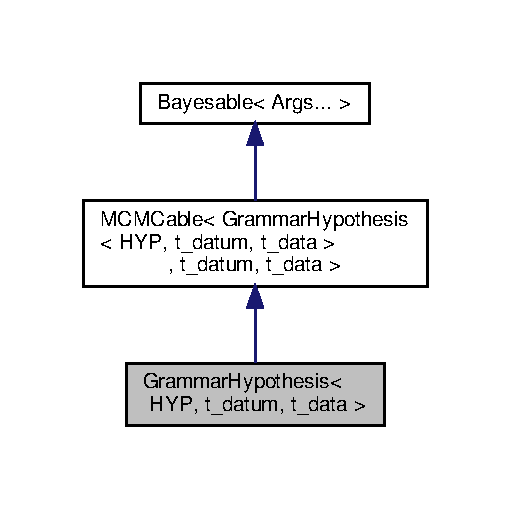
\includegraphics[width=245pt]{class_grammar_hypothesis__inherit__graph}
\end{center}
\end{figure}


Collaboration diagram for Grammar\+Hypothesis$<$ H\+YP, t\+\_\+datum, t\+\_\+data $>$\+:\nopagebreak
\begin{figure}[H]
\begin{center}
\leavevmode
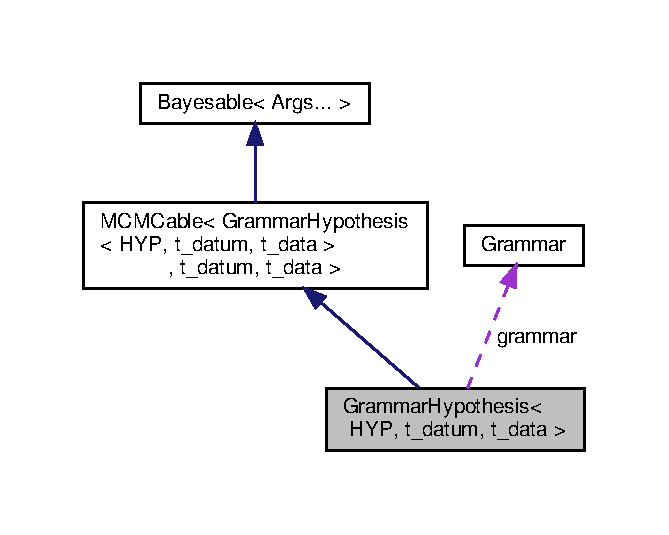
\includegraphics[width=321pt]{class_grammar_hypothesis__coll__graph}
\end{center}
\end{figure}
\subsection*{Public Member Functions}
\begin{DoxyCompactItemize}
\item 
\hyperlink{class_grammar_hypothesis_afd02b96535124c5e205ce7185c64c862}{Grammar\+Hypothesis} ()
\item 
\hyperlink{class_grammar_hypothesis_afe25b747b37d7ae984f9d3e4187484d8}{Grammar\+Hypothesis} (\hyperlink{class_grammar}{Grammar} $\ast$g, \hyperlink{_eigen_numerics_8h_a645222978e81acfb2523a9bce34aecc0}{Matrix} $\ast$c, \hyperlink{_eigen_numerics_8h_a645222978e81acfb2523a9bce34aecc0}{Matrix} $\ast$ll, \hyperlink{_eigen_numerics_8h_a645222978e81acfb2523a9bce34aecc0}{Matrix} $\ast$p)
\item 
\hyperlink{_eigen_numerics_8h_aca2956bc379bce2ed88ab3c0e1b61d1d}{Vector} \& \hyperlink{class_grammar_hypothesis_a379e7af54d3e1cfd5b70f48fcc423470}{getX} ()
\item 
const \hyperlink{_eigen_numerics_8h_aca2956bc379bce2ed88ab3c0e1b61d1d}{Vector} \& \hyperlink{class_grammar_hypothesis_a2e6e231336e00b27bb0a0a1f039d80fa}{getX} () const
\item 
float \hyperlink{class_grammar_hypothesis_aa647148b440db9de4ca97f39c593a0d3}{get\+\_\+baseline} () const
\item 
float \hyperlink{class_grammar_hypothesis_a8ac03e561e97660e21669d0ddb64e028}{get\+\_\+forwardalpha} () const
\item 
double \hyperlink{class_grammar_hypothesis_a11fd75eee387330535601c9ee9d2f0f9}{compute\+\_\+prior} ()
\begin{DoxyCompactList}\small\item\em Compute the prior -- defaultly not defined. \end{DoxyCompactList}\item 
virtual double \hyperlink{class_grammar_hypothesis_a848ed67089c24b55cc61a4d84e350d05}{compute\+\_\+single\+\_\+likelihood} (const \hyperlink{class_bayesable_a7c93a2eeab708378eb321745908718d4}{t\+\_\+datum} \&datum)
\begin{DoxyCompactList}\small\item\em Compute the likelihood of a single data point. \end{DoxyCompactList}\item 
virtual double \hyperlink{class_grammar_hypothesis_ae565db71afc24d042450e9ed471b4908}{compute\+\_\+likelihood} (const \hyperlink{class_bayesable_a70a593a67c7d43239ecc06bb4fd06a6b}{t\+\_\+data} \&data, const double breakout=-\/\hyperlink{_numerics_8h_a1bb1e42ae1b40cad6e99da0aab8a5576}{infinity})
\begin{DoxyCompactList}\small\item\em Compute the likelihood of a collection of data, by calling compute\+\_\+single\+\_\+likelihood on each. This stops if our likelihood falls below breakout. \end{DoxyCompactList}\item 
virtual \hyperlink{class_grammar_hypothesis}{Grammar\+Hypothesis} \hyperlink{class_grammar_hypothesis_a8d0042f4858879ce2585df382ce78b0a}{restart} () const
\item 
virtual std\+::pair$<$ \hyperlink{class_grammar_hypothesis}{Grammar\+Hypothesis}, double $>$ \hyperlink{class_grammar_hypothesis_a5b642e0ccd5c1cebdbd3f7dfdc81cfcf}{propose} () const
\item 
\hyperlink{_eigen_numerics_8h_aca2956bc379bce2ed88ab3c0e1b61d1d}{Vector} \hyperlink{class_grammar_hypothesis_a9fb937f94fbe121dcba164f378e99080}{hypothesis\+\_\+prior} (\hyperlink{_eigen_numerics_8h_a645222978e81acfb2523a9bce34aecc0}{Matrix} \&\hyperlink{class_grammar_hypothesis_a2147efc4d1268e115803bd34f63f1c35}{C})
\item 
virtual bool \hyperlink{class_grammar_hypothesis_a8a64510ebb2af15474bdae7169049c94}{operator==} (const \hyperlink{class_grammar_hypothesis}{Grammar\+Hypothesis}$<$ H\+YP, \hyperlink{class_bayesable_a7c93a2eeab708378eb321745908718d4}{t\+\_\+datum}, \hyperlink{class_bayesable_a70a593a67c7d43239ecc06bb4fd06a6b}{t\+\_\+data} $>$ \&h) const
\item 
virtual std\+::string \hyperlink{class_grammar_hypothesis_a75267d7b68cd9b3634f84a464877c07c}{string} () const
\item 
virtual size\+\_\+t \hyperlink{class_grammar_hypothesis_a5b269a5ed433b94f6b2796f30a15fd9e}{hash} () const
\begin{DoxyCompactList}\small\item\em Default hash function. \end{DoxyCompactList}\end{DoxyCompactItemize}
\subsection*{Public Attributes}
\begin{DoxyCompactItemize}
\item 
\hyperlink{_eigen_numerics_8h_aca2956bc379bce2ed88ab3c0e1b61d1d}{Vector} \hyperlink{class_grammar_hypothesis_a27fdb926401378fc46373ee57bb2a21f}{x}
\item 
\hyperlink{class_grammar}{Grammar} $\ast$ \hyperlink{class_grammar_hypothesis_ae3aa5981689e75e3eccc343c838b8f47}{grammar}
\item 
\hyperlink{_eigen_numerics_8h_a645222978e81acfb2523a9bce34aecc0}{Matrix} $\ast$ \hyperlink{class_grammar_hypothesis_a2147efc4d1268e115803bd34f63f1c35}{C}
\item 
\hyperlink{_eigen_numerics_8h_a645222978e81acfb2523a9bce34aecc0}{Matrix} $\ast$ \hyperlink{class_grammar_hypothesis_a90aea1a98b122b01e7a10cc2c7c251d4}{LL}
\item 
\hyperlink{_eigen_numerics_8h_a645222978e81acfb2523a9bce34aecc0}{Matrix} $\ast$ \hyperlink{class_grammar_hypothesis_a7154fb0938913f01dfd85efb76c46250}{P}
\item 
float \hyperlink{class_grammar_hypothesis_a41985a24a133b009328deed14a2b8802}{logodds\+\_\+baseline}
\item 
float \hyperlink{class_grammar_hypothesis_a1027d3f52f4d1adddd923a18fb393955}{logodds\+\_\+forwardalpha}
\end{DoxyCompactItemize}
\subsection*{Additional Inherited Members}


\subsection{Constructor \& Destructor Documentation}
\mbox{\Hypertarget{class_grammar_hypothesis_afd02b96535124c5e205ce7185c64c862}\label{class_grammar_hypothesis_afd02b96535124c5e205ce7185c64c862}} 
\index{Grammar\+Hypothesis@{Grammar\+Hypothesis}!Grammar\+Hypothesis@{Grammar\+Hypothesis}}
\index{Grammar\+Hypothesis@{Grammar\+Hypothesis}!Grammar\+Hypothesis@{Grammar\+Hypothesis}}
\subsubsection{\texorpdfstring{Grammar\+Hypothesis()}{GrammarHypothesis()}\hspace{0.1cm}{\footnotesize\ttfamily [1/2]}}
{\footnotesize\ttfamily template$<$typename H\+YP, typename t\+\_\+datum, typename t\+\_\+data = std\+::vector$<$t\+\_\+datum$>$$>$ \\
\hyperlink{class_grammar_hypothesis}{Grammar\+Hypothesis}$<$ H\+YP, \hyperlink{class_bayesable_a7c93a2eeab708378eb321745908718d4}{t\+\_\+datum}, \hyperlink{class_bayesable_a70a593a67c7d43239ecc06bb4fd06a6b}{t\+\_\+data} $>$\+::\hyperlink{class_grammar_hypothesis}{Grammar\+Hypothesis} (\begin{DoxyParamCaption}{ }\end{DoxyParamCaption})\hspace{0.3cm}{\ttfamily [inline]}}

\mbox{\Hypertarget{class_grammar_hypothesis_afe25b747b37d7ae984f9d3e4187484d8}\label{class_grammar_hypothesis_afe25b747b37d7ae984f9d3e4187484d8}} 
\index{Grammar\+Hypothesis@{Grammar\+Hypothesis}!Grammar\+Hypothesis@{Grammar\+Hypothesis}}
\index{Grammar\+Hypothesis@{Grammar\+Hypothesis}!Grammar\+Hypothesis@{Grammar\+Hypothesis}}
\subsubsection{\texorpdfstring{Grammar\+Hypothesis()}{GrammarHypothesis()}\hspace{0.1cm}{\footnotesize\ttfamily [2/2]}}
{\footnotesize\ttfamily template$<$typename H\+YP, typename t\+\_\+datum, typename t\+\_\+data = std\+::vector$<$t\+\_\+datum$>$$>$ \\
\hyperlink{class_grammar_hypothesis}{Grammar\+Hypothesis}$<$ H\+YP, \hyperlink{class_bayesable_a7c93a2eeab708378eb321745908718d4}{t\+\_\+datum}, \hyperlink{class_bayesable_a70a593a67c7d43239ecc06bb4fd06a6b}{t\+\_\+data} $>$\+::\hyperlink{class_grammar_hypothesis}{Grammar\+Hypothesis} (\begin{DoxyParamCaption}\item[{\hyperlink{class_grammar}{Grammar} $\ast$}]{g,  }\item[{\hyperlink{_eigen_numerics_8h_a645222978e81acfb2523a9bce34aecc0}{Matrix} $\ast$}]{c,  }\item[{\hyperlink{_eigen_numerics_8h_a645222978e81acfb2523a9bce34aecc0}{Matrix} $\ast$}]{ll,  }\item[{\hyperlink{_eigen_numerics_8h_a645222978e81acfb2523a9bce34aecc0}{Matrix} $\ast$}]{p }\end{DoxyParamCaption})\hspace{0.3cm}{\ttfamily [inline]}}



\subsection{Member Function Documentation}
\mbox{\Hypertarget{class_grammar_hypothesis_ae565db71afc24d042450e9ed471b4908}\label{class_grammar_hypothesis_ae565db71afc24d042450e9ed471b4908}} 
\index{Grammar\+Hypothesis@{Grammar\+Hypothesis}!compute\+\_\+likelihood@{compute\+\_\+likelihood}}
\index{compute\+\_\+likelihood@{compute\+\_\+likelihood}!Grammar\+Hypothesis@{Grammar\+Hypothesis}}
\subsubsection{\texorpdfstring{compute\+\_\+likelihood()}{compute\_likelihood()}}
{\footnotesize\ttfamily template$<$typename H\+YP, typename t\+\_\+datum, typename t\+\_\+data = std\+::vector$<$t\+\_\+datum$>$$>$ \\
virtual double \hyperlink{class_grammar_hypothesis}{Grammar\+Hypothesis}$<$ H\+YP, \hyperlink{class_bayesable_a7c93a2eeab708378eb321745908718d4}{t\+\_\+datum}, \hyperlink{class_bayesable_a70a593a67c7d43239ecc06bb4fd06a6b}{t\+\_\+data} $>$\+::compute\+\_\+likelihood (\begin{DoxyParamCaption}\item[{const \hyperlink{class_bayesable_a70a593a67c7d43239ecc06bb4fd06a6b}{t\+\_\+data} \&}]{data,  }\item[{const double}]{breakout = {\ttfamily -\/\hyperlink{_numerics_8h_a1bb1e42ae1b40cad6e99da0aab8a5576}{infinity}} }\end{DoxyParamCaption})\hspace{0.3cm}{\ttfamily [inline]}, {\ttfamily [virtual]}}



Compute the likelihood of a collection of data, by calling compute\+\_\+single\+\_\+likelihood on each. This stops if our likelihood falls below breakout. 


\begin{DoxyParams}{Parameters}
{\em data} & \\
\hline
{\em breakout} & \\
\hline
\end{DoxyParams}
\begin{DoxyReturn}{Returns}

\end{DoxyReturn}


Reimplemented from \hyperlink{class_bayesable_af9547335ae15a5068b10d29aee5056ae}{Bayesable$<$ Args... $>$}.

\mbox{\Hypertarget{class_grammar_hypothesis_a11fd75eee387330535601c9ee9d2f0f9}\label{class_grammar_hypothesis_a11fd75eee387330535601c9ee9d2f0f9}} 
\index{Grammar\+Hypothesis@{Grammar\+Hypothesis}!compute\+\_\+prior@{compute\+\_\+prior}}
\index{compute\+\_\+prior@{compute\+\_\+prior}!Grammar\+Hypothesis@{Grammar\+Hypothesis}}
\subsubsection{\texorpdfstring{compute\+\_\+prior()}{compute\_prior()}}
{\footnotesize\ttfamily template$<$typename H\+YP, typename t\+\_\+datum, typename t\+\_\+data = std\+::vector$<$t\+\_\+datum$>$$>$ \\
double \hyperlink{class_grammar_hypothesis}{Grammar\+Hypothesis}$<$ H\+YP, \hyperlink{class_bayesable_a7c93a2eeab708378eb321745908718d4}{t\+\_\+datum}, \hyperlink{class_bayesable_a70a593a67c7d43239ecc06bb4fd06a6b}{t\+\_\+data} $>$\+::compute\+\_\+prior (\begin{DoxyParamCaption}{ }\end{DoxyParamCaption})\hspace{0.3cm}{\ttfamily [inline]}, {\ttfamily [virtual]}}



Compute the prior -- defaultly not defined. 



Implements \hyperlink{class_bayesable_a9aa752f0adff1b95f8957b91fc928649}{Bayesable$<$ Args... $>$}.

\mbox{\Hypertarget{class_grammar_hypothesis_a848ed67089c24b55cc61a4d84e350d05}\label{class_grammar_hypothesis_a848ed67089c24b55cc61a4d84e350d05}} 
\index{Grammar\+Hypothesis@{Grammar\+Hypothesis}!compute\+\_\+single\+\_\+likelihood@{compute\+\_\+single\+\_\+likelihood}}
\index{compute\+\_\+single\+\_\+likelihood@{compute\+\_\+single\+\_\+likelihood}!Grammar\+Hypothesis@{Grammar\+Hypothesis}}
\subsubsection{\texorpdfstring{compute\+\_\+single\+\_\+likelihood()}{compute\_single\_likelihood()}}
{\footnotesize\ttfamily template$<$typename H\+YP, typename t\+\_\+datum, typename t\+\_\+data = std\+::vector$<$t\+\_\+datum$>$$>$ \\
virtual double \hyperlink{class_grammar_hypothesis}{Grammar\+Hypothesis}$<$ H\+YP, \hyperlink{class_bayesable_a7c93a2eeab708378eb321745908718d4}{t\+\_\+datum}, \hyperlink{class_bayesable_a70a593a67c7d43239ecc06bb4fd06a6b}{t\+\_\+data} $>$\+::compute\+\_\+single\+\_\+likelihood (\begin{DoxyParamCaption}\item[{const \hyperlink{class_bayesable_a7c93a2eeab708378eb321745908718d4}{t\+\_\+datum} \&}]{datum }\end{DoxyParamCaption})\hspace{0.3cm}{\ttfamily [inline]}, {\ttfamily [virtual]}}



Compute the likelihood of a single data point. 


\begin{DoxyParams}{Parameters}
{\em datum} & \\
\hline
\end{DoxyParams}


Implements \hyperlink{class_bayesable_a5e0237ec7a40a2c45c990f93a8dc8e00}{Bayesable$<$ Args... $>$}.

\mbox{\Hypertarget{class_grammar_hypothesis_aa647148b440db9de4ca97f39c593a0d3}\label{class_grammar_hypothesis_aa647148b440db9de4ca97f39c593a0d3}} 
\index{Grammar\+Hypothesis@{Grammar\+Hypothesis}!get\+\_\+baseline@{get\+\_\+baseline}}
\index{get\+\_\+baseline@{get\+\_\+baseline}!Grammar\+Hypothesis@{Grammar\+Hypothesis}}
\subsubsection{\texorpdfstring{get\+\_\+baseline()}{get\_baseline()}}
{\footnotesize\ttfamily template$<$typename H\+YP, typename t\+\_\+datum, typename t\+\_\+data = std\+::vector$<$t\+\_\+datum$>$$>$ \\
float \hyperlink{class_grammar_hypothesis}{Grammar\+Hypothesis}$<$ H\+YP, \hyperlink{class_bayesable_a7c93a2eeab708378eb321745908718d4}{t\+\_\+datum}, \hyperlink{class_bayesable_a70a593a67c7d43239ecc06bb4fd06a6b}{t\+\_\+data} $>$\+::get\+\_\+baseline (\begin{DoxyParamCaption}{ }\end{DoxyParamCaption}) const\hspace{0.3cm}{\ttfamily [inline]}}

\mbox{\Hypertarget{class_grammar_hypothesis_a8ac03e561e97660e21669d0ddb64e028}\label{class_grammar_hypothesis_a8ac03e561e97660e21669d0ddb64e028}} 
\index{Grammar\+Hypothesis@{Grammar\+Hypothesis}!get\+\_\+forwardalpha@{get\+\_\+forwardalpha}}
\index{get\+\_\+forwardalpha@{get\+\_\+forwardalpha}!Grammar\+Hypothesis@{Grammar\+Hypothesis}}
\subsubsection{\texorpdfstring{get\+\_\+forwardalpha()}{get\_forwardalpha()}}
{\footnotesize\ttfamily template$<$typename H\+YP, typename t\+\_\+datum, typename t\+\_\+data = std\+::vector$<$t\+\_\+datum$>$$>$ \\
float \hyperlink{class_grammar_hypothesis}{Grammar\+Hypothesis}$<$ H\+YP, \hyperlink{class_bayesable_a7c93a2eeab708378eb321745908718d4}{t\+\_\+datum}, \hyperlink{class_bayesable_a70a593a67c7d43239ecc06bb4fd06a6b}{t\+\_\+data} $>$\+::get\+\_\+forwardalpha (\begin{DoxyParamCaption}{ }\end{DoxyParamCaption}) const\hspace{0.3cm}{\ttfamily [inline]}}

\mbox{\Hypertarget{class_grammar_hypothesis_a379e7af54d3e1cfd5b70f48fcc423470}\label{class_grammar_hypothesis_a379e7af54d3e1cfd5b70f48fcc423470}} 
\index{Grammar\+Hypothesis@{Grammar\+Hypothesis}!getX@{getX}}
\index{getX@{getX}!Grammar\+Hypothesis@{Grammar\+Hypothesis}}
\subsubsection{\texorpdfstring{get\+X()}{getX()}\hspace{0.1cm}{\footnotesize\ttfamily [1/2]}}
{\footnotesize\ttfamily template$<$typename H\+YP, typename t\+\_\+datum, typename t\+\_\+data = std\+::vector$<$t\+\_\+datum$>$$>$ \\
\hyperlink{_eigen_numerics_8h_aca2956bc379bce2ed88ab3c0e1b61d1d}{Vector}\& \hyperlink{class_grammar_hypothesis}{Grammar\+Hypothesis}$<$ H\+YP, \hyperlink{class_bayesable_a7c93a2eeab708378eb321745908718d4}{t\+\_\+datum}, \hyperlink{class_bayesable_a70a593a67c7d43239ecc06bb4fd06a6b}{t\+\_\+data} $>$\+::getX (\begin{DoxyParamCaption}{ }\end{DoxyParamCaption})\hspace{0.3cm}{\ttfamily [inline]}}

\mbox{\Hypertarget{class_grammar_hypothesis_a2e6e231336e00b27bb0a0a1f039d80fa}\label{class_grammar_hypothesis_a2e6e231336e00b27bb0a0a1f039d80fa}} 
\index{Grammar\+Hypothesis@{Grammar\+Hypothesis}!getX@{getX}}
\index{getX@{getX}!Grammar\+Hypothesis@{Grammar\+Hypothesis}}
\subsubsection{\texorpdfstring{get\+X()}{getX()}\hspace{0.1cm}{\footnotesize\ttfamily [2/2]}}
{\footnotesize\ttfamily template$<$typename H\+YP, typename t\+\_\+datum, typename t\+\_\+data = std\+::vector$<$t\+\_\+datum$>$$>$ \\
const \hyperlink{_eigen_numerics_8h_aca2956bc379bce2ed88ab3c0e1b61d1d}{Vector}\& \hyperlink{class_grammar_hypothesis}{Grammar\+Hypothesis}$<$ H\+YP, \hyperlink{class_bayesable_a7c93a2eeab708378eb321745908718d4}{t\+\_\+datum}, \hyperlink{class_bayesable_a70a593a67c7d43239ecc06bb4fd06a6b}{t\+\_\+data} $>$\+::getX (\begin{DoxyParamCaption}{ }\end{DoxyParamCaption}) const\hspace{0.3cm}{\ttfamily [inline]}}

\mbox{\Hypertarget{class_grammar_hypothesis_a5b269a5ed433b94f6b2796f30a15fd9e}\label{class_grammar_hypothesis_a5b269a5ed433b94f6b2796f30a15fd9e}} 
\index{Grammar\+Hypothesis@{Grammar\+Hypothesis}!hash@{hash}}
\index{hash@{hash}!Grammar\+Hypothesis@{Grammar\+Hypothesis}}
\subsubsection{\texorpdfstring{hash()}{hash()}}
{\footnotesize\ttfamily template$<$typename H\+YP, typename t\+\_\+datum, typename t\+\_\+data = std\+::vector$<$t\+\_\+datum$>$$>$ \\
virtual size\+\_\+t \hyperlink{class_grammar_hypothesis}{Grammar\+Hypothesis}$<$ H\+YP, \hyperlink{class_bayesable_a7c93a2eeab708378eb321745908718d4}{t\+\_\+datum}, \hyperlink{class_bayesable_a70a593a67c7d43239ecc06bb4fd06a6b}{t\+\_\+data} $>$\+::hash (\begin{DoxyParamCaption}{ }\end{DoxyParamCaption}) const\hspace{0.3cm}{\ttfamily [inline]}, {\ttfamily [virtual]}}



Default hash function. 



Implements \hyperlink{class_bayesable_ab77a023d33951448e6edb2e1bc79c5ae}{Bayesable$<$ Args... $>$}.

\mbox{\Hypertarget{class_grammar_hypothesis_a9fb937f94fbe121dcba164f378e99080}\label{class_grammar_hypothesis_a9fb937f94fbe121dcba164f378e99080}} 
\index{Grammar\+Hypothesis@{Grammar\+Hypothesis}!hypothesis\+\_\+prior@{hypothesis\+\_\+prior}}
\index{hypothesis\+\_\+prior@{hypothesis\+\_\+prior}!Grammar\+Hypothesis@{Grammar\+Hypothesis}}
\subsubsection{\texorpdfstring{hypothesis\+\_\+prior()}{hypothesis\_prior()}}
{\footnotesize\ttfamily template$<$typename H\+YP, typename t\+\_\+datum, typename t\+\_\+data = std\+::vector$<$t\+\_\+datum$>$$>$ \\
\hyperlink{_eigen_numerics_8h_aca2956bc379bce2ed88ab3c0e1b61d1d}{Vector} \hyperlink{class_grammar_hypothesis}{Grammar\+Hypothesis}$<$ H\+YP, \hyperlink{class_bayesable_a7c93a2eeab708378eb321745908718d4}{t\+\_\+datum}, \hyperlink{class_bayesable_a70a593a67c7d43239ecc06bb4fd06a6b}{t\+\_\+data} $>$\+::hypothesis\+\_\+prior (\begin{DoxyParamCaption}\item[{\hyperlink{_eigen_numerics_8h_a645222978e81acfb2523a9bce34aecc0}{Matrix} \&}]{C }\end{DoxyParamCaption})\hspace{0.3cm}{\ttfamily [inline]}}

\mbox{\Hypertarget{class_grammar_hypothesis_a8a64510ebb2af15474bdae7169049c94}\label{class_grammar_hypothesis_a8a64510ebb2af15474bdae7169049c94}} 
\index{Grammar\+Hypothesis@{Grammar\+Hypothesis}!operator==@{operator==}}
\index{operator==@{operator==}!Grammar\+Hypothesis@{Grammar\+Hypothesis}}
\subsubsection{\texorpdfstring{operator==()}{operator==()}}
{\footnotesize\ttfamily template$<$typename H\+YP, typename t\+\_\+datum, typename t\+\_\+data = std\+::vector$<$t\+\_\+datum$>$$>$ \\
virtual bool \hyperlink{class_grammar_hypothesis}{Grammar\+Hypothesis}$<$ H\+YP, \hyperlink{class_bayesable_a7c93a2eeab708378eb321745908718d4}{t\+\_\+datum}, \hyperlink{class_bayesable_a70a593a67c7d43239ecc06bb4fd06a6b}{t\+\_\+data} $>$\+::operator== (\begin{DoxyParamCaption}\item[{const \hyperlink{class_grammar_hypothesis}{Grammar\+Hypothesis}$<$ H\+YP, \hyperlink{class_bayesable_a7c93a2eeab708378eb321745908718d4}{t\+\_\+datum}, \hyperlink{class_bayesable_a70a593a67c7d43239ecc06bb4fd06a6b}{t\+\_\+data} $>$ \&}]{h }\end{DoxyParamCaption}) const\hspace{0.3cm}{\ttfamily [inline]}, {\ttfamily [virtual]}}



Implements \hyperlink{class_m_c_m_cable_aa73001ec3bb0cf0c618281dfa998f2f1}{M\+C\+M\+Cable$<$ Grammar\+Hypothesis$<$ H\+Y\+P, t\+\_\+datum, t\+\_\+data $>$, t\+\_\+datum, t\+\_\+data $>$}.

\mbox{\Hypertarget{class_grammar_hypothesis_a5b642e0ccd5c1cebdbd3f7dfdc81cfcf}\label{class_grammar_hypothesis_a5b642e0ccd5c1cebdbd3f7dfdc81cfcf}} 
\index{Grammar\+Hypothesis@{Grammar\+Hypothesis}!propose@{propose}}
\index{propose@{propose}!Grammar\+Hypothesis@{Grammar\+Hypothesis}}
\subsubsection{\texorpdfstring{propose()}{propose()}}
{\footnotesize\ttfamily template$<$typename H\+YP, typename t\+\_\+datum, typename t\+\_\+data = std\+::vector$<$t\+\_\+datum$>$$>$ \\
virtual std\+::pair$<$\hyperlink{class_grammar_hypothesis}{Grammar\+Hypothesis},double$>$ \hyperlink{class_grammar_hypothesis}{Grammar\+Hypothesis}$<$ H\+YP, \hyperlink{class_bayesable_a7c93a2eeab708378eb321745908718d4}{t\+\_\+datum}, \hyperlink{class_bayesable_a70a593a67c7d43239ecc06bb4fd06a6b}{t\+\_\+data} $>$\+::propose (\begin{DoxyParamCaption}{ }\end{DoxyParamCaption}) const\hspace{0.3cm}{\ttfamily [inline]}, {\ttfamily [virtual]}}



Implements \hyperlink{class_m_c_m_cable_ab119a14256ab92c5c1e941f8492df830}{M\+C\+M\+Cable$<$ Grammar\+Hypothesis$<$ H\+Y\+P, t\+\_\+datum, t\+\_\+data $>$, t\+\_\+datum, t\+\_\+data $>$}.

\mbox{\Hypertarget{class_grammar_hypothesis_a8d0042f4858879ce2585df382ce78b0a}\label{class_grammar_hypothesis_a8d0042f4858879ce2585df382ce78b0a}} 
\index{Grammar\+Hypothesis@{Grammar\+Hypothesis}!restart@{restart}}
\index{restart@{restart}!Grammar\+Hypothesis@{Grammar\+Hypothesis}}
\subsubsection{\texorpdfstring{restart()}{restart()}}
{\footnotesize\ttfamily template$<$typename H\+YP, typename t\+\_\+datum, typename t\+\_\+data = std\+::vector$<$t\+\_\+datum$>$$>$ \\
virtual \hyperlink{class_grammar_hypothesis}{Grammar\+Hypothesis} \hyperlink{class_grammar_hypothesis}{Grammar\+Hypothesis}$<$ H\+YP, \hyperlink{class_bayesable_a7c93a2eeab708378eb321745908718d4}{t\+\_\+datum}, \hyperlink{class_bayesable_a70a593a67c7d43239ecc06bb4fd06a6b}{t\+\_\+data} $>$\+::restart (\begin{DoxyParamCaption}{ }\end{DoxyParamCaption}) const\hspace{0.3cm}{\ttfamily [inline]}, {\ttfamily [virtual]}}



Implements \hyperlink{class_m_c_m_cable_a220d6c4ca73e20441c14fa5bd3e090d3}{M\+C\+M\+Cable$<$ Grammar\+Hypothesis$<$ H\+Y\+P, t\+\_\+datum, t\+\_\+data $>$, t\+\_\+datum, t\+\_\+data $>$}.

\mbox{\Hypertarget{class_grammar_hypothesis_a75267d7b68cd9b3634f84a464877c07c}\label{class_grammar_hypothesis_a75267d7b68cd9b3634f84a464877c07c}} 
\index{Grammar\+Hypothesis@{Grammar\+Hypothesis}!string@{string}}
\index{string@{string}!Grammar\+Hypothesis@{Grammar\+Hypothesis}}
\subsubsection{\texorpdfstring{string()}{string()}}
{\footnotesize\ttfamily template$<$typename H\+YP, typename t\+\_\+datum, typename t\+\_\+data = std\+::vector$<$t\+\_\+datum$>$$>$ \\
virtual std\+::string \hyperlink{class_grammar_hypothesis}{Grammar\+Hypothesis}$<$ H\+YP, \hyperlink{class_bayesable_a7c93a2eeab708378eb321745908718d4}{t\+\_\+datum}, \hyperlink{class_bayesable_a70a593a67c7d43239ecc06bb4fd06a6b}{t\+\_\+data} $>$\+::string (\begin{DoxyParamCaption}{ }\end{DoxyParamCaption}) const\hspace{0.3cm}{\ttfamily [inline]}, {\ttfamily [virtual]}}



Implements \hyperlink{class_bayesable_a2ec58e98bf37a90ac3d45a7713c6d5ea}{Bayesable$<$ Args... $>$}.



\subsection{Member Data Documentation}
\mbox{\Hypertarget{class_grammar_hypothesis_a2147efc4d1268e115803bd34f63f1c35}\label{class_grammar_hypothesis_a2147efc4d1268e115803bd34f63f1c35}} 
\index{Grammar\+Hypothesis@{Grammar\+Hypothesis}!C@{C}}
\index{C@{C}!Grammar\+Hypothesis@{Grammar\+Hypothesis}}
\subsubsection{\texorpdfstring{C}{C}}
{\footnotesize\ttfamily template$<$typename H\+YP, typename t\+\_\+datum, typename t\+\_\+data = std\+::vector$<$t\+\_\+datum$>$$>$ \\
\hyperlink{_eigen_numerics_8h_a645222978e81acfb2523a9bce34aecc0}{Matrix}$\ast$ \hyperlink{class_grammar_hypothesis}{Grammar\+Hypothesis}$<$ H\+YP, \hyperlink{class_bayesable_a7c93a2eeab708378eb321745908718d4}{t\+\_\+datum}, \hyperlink{class_bayesable_a70a593a67c7d43239ecc06bb4fd06a6b}{t\+\_\+data} $>$\+::C}

\mbox{\Hypertarget{class_grammar_hypothesis_ae3aa5981689e75e3eccc343c838b8f47}\label{class_grammar_hypothesis_ae3aa5981689e75e3eccc343c838b8f47}} 
\index{Grammar\+Hypothesis@{Grammar\+Hypothesis}!grammar@{grammar}}
\index{grammar@{grammar}!Grammar\+Hypothesis@{Grammar\+Hypothesis}}
\subsubsection{\texorpdfstring{grammar}{grammar}}
{\footnotesize\ttfamily template$<$typename H\+YP, typename t\+\_\+datum, typename t\+\_\+data = std\+::vector$<$t\+\_\+datum$>$$>$ \\
\hyperlink{class_grammar}{Grammar}$\ast$ \hyperlink{class_grammar_hypothesis}{Grammar\+Hypothesis}$<$ H\+YP, \hyperlink{class_bayesable_a7c93a2eeab708378eb321745908718d4}{t\+\_\+datum}, \hyperlink{class_bayesable_a70a593a67c7d43239ecc06bb4fd06a6b}{t\+\_\+data} $>$\+::grammar}

\mbox{\Hypertarget{class_grammar_hypothesis_a90aea1a98b122b01e7a10cc2c7c251d4}\label{class_grammar_hypothesis_a90aea1a98b122b01e7a10cc2c7c251d4}} 
\index{Grammar\+Hypothesis@{Grammar\+Hypothesis}!LL@{LL}}
\index{LL@{LL}!Grammar\+Hypothesis@{Grammar\+Hypothesis}}
\subsubsection{\texorpdfstring{LL}{LL}}
{\footnotesize\ttfamily template$<$typename H\+YP, typename t\+\_\+datum, typename t\+\_\+data = std\+::vector$<$t\+\_\+datum$>$$>$ \\
\hyperlink{_eigen_numerics_8h_a645222978e81acfb2523a9bce34aecc0}{Matrix}$\ast$ \hyperlink{class_grammar_hypothesis}{Grammar\+Hypothesis}$<$ H\+YP, \hyperlink{class_bayesable_a7c93a2eeab708378eb321745908718d4}{t\+\_\+datum}, \hyperlink{class_bayesable_a70a593a67c7d43239ecc06bb4fd06a6b}{t\+\_\+data} $>$\+::LL}

\mbox{\Hypertarget{class_grammar_hypothesis_a41985a24a133b009328deed14a2b8802}\label{class_grammar_hypothesis_a41985a24a133b009328deed14a2b8802}} 
\index{Grammar\+Hypothesis@{Grammar\+Hypothesis}!logodds\+\_\+baseline@{logodds\+\_\+baseline}}
\index{logodds\+\_\+baseline@{logodds\+\_\+baseline}!Grammar\+Hypothesis@{Grammar\+Hypothesis}}
\subsubsection{\texorpdfstring{logodds\+\_\+baseline}{logodds\_baseline}}
{\footnotesize\ttfamily template$<$typename H\+YP, typename t\+\_\+datum, typename t\+\_\+data = std\+::vector$<$t\+\_\+datum$>$$>$ \\
float \hyperlink{class_grammar_hypothesis}{Grammar\+Hypothesis}$<$ H\+YP, \hyperlink{class_bayesable_a7c93a2eeab708378eb321745908718d4}{t\+\_\+datum}, \hyperlink{class_bayesable_a70a593a67c7d43239ecc06bb4fd06a6b}{t\+\_\+data} $>$\+::logodds\+\_\+baseline}

\mbox{\Hypertarget{class_grammar_hypothesis_a1027d3f52f4d1adddd923a18fb393955}\label{class_grammar_hypothesis_a1027d3f52f4d1adddd923a18fb393955}} 
\index{Grammar\+Hypothesis@{Grammar\+Hypothesis}!logodds\+\_\+forwardalpha@{logodds\+\_\+forwardalpha}}
\index{logodds\+\_\+forwardalpha@{logodds\+\_\+forwardalpha}!Grammar\+Hypothesis@{Grammar\+Hypothesis}}
\subsubsection{\texorpdfstring{logodds\+\_\+forwardalpha}{logodds\_forwardalpha}}
{\footnotesize\ttfamily template$<$typename H\+YP, typename t\+\_\+datum, typename t\+\_\+data = std\+::vector$<$t\+\_\+datum$>$$>$ \\
float \hyperlink{class_grammar_hypothesis}{Grammar\+Hypothesis}$<$ H\+YP, \hyperlink{class_bayesable_a7c93a2eeab708378eb321745908718d4}{t\+\_\+datum}, \hyperlink{class_bayesable_a70a593a67c7d43239ecc06bb4fd06a6b}{t\+\_\+data} $>$\+::logodds\+\_\+forwardalpha}

\mbox{\Hypertarget{class_grammar_hypothesis_a7154fb0938913f01dfd85efb76c46250}\label{class_grammar_hypothesis_a7154fb0938913f01dfd85efb76c46250}} 
\index{Grammar\+Hypothesis@{Grammar\+Hypothesis}!P@{P}}
\index{P@{P}!Grammar\+Hypothesis@{Grammar\+Hypothesis}}
\subsubsection{\texorpdfstring{P}{P}}
{\footnotesize\ttfamily template$<$typename H\+YP, typename t\+\_\+datum, typename t\+\_\+data = std\+::vector$<$t\+\_\+datum$>$$>$ \\
\hyperlink{_eigen_numerics_8h_a645222978e81acfb2523a9bce34aecc0}{Matrix}$\ast$ \hyperlink{class_grammar_hypothesis}{Grammar\+Hypothesis}$<$ H\+YP, \hyperlink{class_bayesable_a7c93a2eeab708378eb321745908718d4}{t\+\_\+datum}, \hyperlink{class_bayesable_a70a593a67c7d43239ecc06bb4fd06a6b}{t\+\_\+data} $>$\+::P}

\mbox{\Hypertarget{class_grammar_hypothesis_a27fdb926401378fc46373ee57bb2a21f}\label{class_grammar_hypothesis_a27fdb926401378fc46373ee57bb2a21f}} 
\index{Grammar\+Hypothesis@{Grammar\+Hypothesis}!x@{x}}
\index{x@{x}!Grammar\+Hypothesis@{Grammar\+Hypothesis}}
\subsubsection{\texorpdfstring{x}{x}}
{\footnotesize\ttfamily template$<$typename H\+YP, typename t\+\_\+datum, typename t\+\_\+data = std\+::vector$<$t\+\_\+datum$>$$>$ \\
\hyperlink{_eigen_numerics_8h_aca2956bc379bce2ed88ab3c0e1b61d1d}{Vector} \hyperlink{class_grammar_hypothesis}{Grammar\+Hypothesis}$<$ H\+YP, \hyperlink{class_bayesable_a7c93a2eeab708378eb321745908718d4}{t\+\_\+datum}, \hyperlink{class_bayesable_a70a593a67c7d43239ecc06bb4fd06a6b}{t\+\_\+data} $>$\+::x}



The documentation for this class was generated from the following file\+:\begin{DoxyCompactItemize}
\item 
src/\+Hypotheses/\hyperlink{_grammar_hypothesis_8h}{Grammar\+Hypothesis.\+h}\end{DoxyCompactItemize}

\input{struct_has_posterior}
\input{struct_has_posterior_3_01_t_00_01decltype_07_07void_08_01_t_1_1posterior_00_010_08_4}
\hypertarget{struct_human_datum}{}\section{Human\+Datum$<$ t\+\_\+learnerdatum, t\+\_\+learnerdata $>$ Struct Template Reference}
\label{struct_human_datum}\index{Human\+Datum$<$ t\+\_\+learnerdatum, t\+\_\+learnerdata $>$@{Human\+Datum$<$ t\+\_\+learnerdatum, t\+\_\+learnerdata $>$}}


{\ttfamily \#include $<$Grammar\+Hypothesis.\+h$>$}

\subsection*{Public Attributes}
\begin{DoxyCompactItemize}
\item 
size\+\_\+t \hyperlink{struct_human_datum_a3569e7634ea9badbe48105cb3a4e5800}{cntyes}
\item 
size\+\_\+t \hyperlink{struct_human_datum_a713ec5993bc2a348a73f292865a6ddcf}{cntno}
\item 
t\+\_\+learnerdata \hyperlink{struct_human_datum_aab13b229dfedb8c2466f47a58e710431}{given\+\_\+data}
\item 
t\+\_\+learnerdatum \hyperlink{struct_human_datum_ab4676fce2bedc28aca179a17fce99be2}{predict\+\_\+data}
\end{DoxyCompactItemize}


\subsection{Member Data Documentation}
\mbox{\Hypertarget{struct_human_datum_a713ec5993bc2a348a73f292865a6ddcf}\label{struct_human_datum_a713ec5993bc2a348a73f292865a6ddcf}} 
\index{Human\+Datum@{Human\+Datum}!cntno@{cntno}}
\index{cntno@{cntno}!Human\+Datum@{Human\+Datum}}
\subsubsection{\texorpdfstring{cntno}{cntno}}
{\footnotesize\ttfamily template$<$typename t\+\_\+learnerdatum , typename t\+\_\+learnerdata  = std\+::vector$<$t\+\_\+learnerdatum$>$$>$ \\
size\+\_\+t \hyperlink{struct_human_datum}{Human\+Datum}$<$ t\+\_\+learnerdatum, t\+\_\+learnerdata $>$\+::cntno}

\mbox{\Hypertarget{struct_human_datum_a3569e7634ea9badbe48105cb3a4e5800}\label{struct_human_datum_a3569e7634ea9badbe48105cb3a4e5800}} 
\index{Human\+Datum@{Human\+Datum}!cntyes@{cntyes}}
\index{cntyes@{cntyes}!Human\+Datum@{Human\+Datum}}
\subsubsection{\texorpdfstring{cntyes}{cntyes}}
{\footnotesize\ttfamily template$<$typename t\+\_\+learnerdatum , typename t\+\_\+learnerdata  = std\+::vector$<$t\+\_\+learnerdatum$>$$>$ \\
size\+\_\+t \hyperlink{struct_human_datum}{Human\+Datum}$<$ t\+\_\+learnerdatum, t\+\_\+learnerdata $>$\+::cntyes}

\mbox{\Hypertarget{struct_human_datum_aab13b229dfedb8c2466f47a58e710431}\label{struct_human_datum_aab13b229dfedb8c2466f47a58e710431}} 
\index{Human\+Datum@{Human\+Datum}!given\+\_\+data@{given\+\_\+data}}
\index{given\+\_\+data@{given\+\_\+data}!Human\+Datum@{Human\+Datum}}
\subsubsection{\texorpdfstring{given\+\_\+data}{given\_data}}
{\footnotesize\ttfamily template$<$typename t\+\_\+learnerdatum , typename t\+\_\+learnerdata  = std\+::vector$<$t\+\_\+learnerdatum$>$$>$ \\
t\+\_\+learnerdata \hyperlink{struct_human_datum}{Human\+Datum}$<$ t\+\_\+learnerdatum, t\+\_\+learnerdata $>$\+::given\+\_\+data}

\mbox{\Hypertarget{struct_human_datum_ab4676fce2bedc28aca179a17fce99be2}\label{struct_human_datum_ab4676fce2bedc28aca179a17fce99be2}} 
\index{Human\+Datum@{Human\+Datum}!predict\+\_\+data@{predict\+\_\+data}}
\index{predict\+\_\+data@{predict\+\_\+data}!Human\+Datum@{Human\+Datum}}
\subsubsection{\texorpdfstring{predict\+\_\+data}{predict\_data}}
{\footnotesize\ttfamily template$<$typename t\+\_\+learnerdatum , typename t\+\_\+learnerdata  = std\+::vector$<$t\+\_\+learnerdatum$>$$>$ \\
t\+\_\+learnerdatum \hyperlink{struct_human_datum}{Human\+Datum}$<$ t\+\_\+learnerdatum, t\+\_\+learnerdata $>$\+::predict\+\_\+data}



The documentation for this struct was generated from the following file\+:\begin{DoxyCompactItemize}
\item 
src/\+Hypotheses/\hyperlink{_grammar_hypothesis_8h}{Grammar\+Hypothesis.\+h}\end{DoxyCompactItemize}

\hypertarget{struct_builtin_1_1_if}{}\section{Builtin\+:\+:If$<$ t $>$ Struct Template Reference}
\label{struct_builtin_1_1_if}\index{Builtin\+::\+If$<$ t $>$@{Builtin\+::\+If$<$ t $>$}}


{\ttfamily \#include $<$Builtins.\+h$>$}



Inheritance diagram for Builtin\+:\+:If$<$ t $>$\+:\nopagebreak
\begin{figure}[H]
\begin{center}
\leavevmode
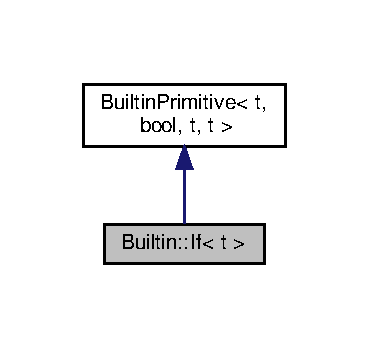
\includegraphics[width=177pt]{struct_builtin_1_1_if__inherit__graph}
\end{center}
\end{figure}


Collaboration diagram for Builtin\+:\+:If$<$ t $>$\+:\nopagebreak
\begin{figure}[H]
\begin{center}
\leavevmode
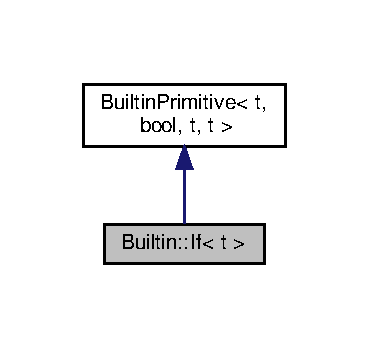
\includegraphics[width=177pt]{struct_builtin_1_1_if__coll__graph}
\end{center}
\end{figure}
\subsection*{Public Member Functions}
\begin{DoxyCompactItemize}
\item 
\hyperlink{struct_builtin_1_1_if_a4ea649fb18a5c42445c5c48e8549c951}{If} (std\+::string fmt, double \+\_\+p=1.\+0)
\end{DoxyCompactItemize}
\subsection*{Additional Inherited Members}


\subsection{Constructor \& Destructor Documentation}
\mbox{\Hypertarget{struct_builtin_1_1_if_a4ea649fb18a5c42445c5c48e8549c951}\label{struct_builtin_1_1_if_a4ea649fb18a5c42445c5c48e8549c951}} 
\index{Builtin\+::\+If@{Builtin\+::\+If}!If@{If}}
\index{If@{If}!Builtin\+::\+If@{Builtin\+::\+If}}
\subsubsection{\texorpdfstring{If()}{If()}}
{\footnotesize\ttfamily template$<$typename t $>$ \\
\hyperlink{struct_builtin_1_1_if}{Builtin\+::\+If}$<$ t $>$\+::\hyperlink{struct_builtin_1_1_if}{If} (\begin{DoxyParamCaption}\item[{std\+::string}]{fmt,  }\item[{double}]{\+\_\+p = {\ttfamily 1.0} }\end{DoxyParamCaption})\hspace{0.3cm}{\ttfamily [inline]}}



The documentation for this struct was generated from the following file\+:\begin{DoxyCompactItemize}
\item 
src/\+Virtual\+Machine/\hyperlink{_builtins_8h}{Builtins.\+h}\end{DoxyCompactItemize}

\hypertarget{class_inner_hypothesis}{}\section{Inner\+Hypothesis Class Reference}
\label{class_inner_hypothesis}\index{Inner\+Hypothesis@{Inner\+Hypothesis}}


Inheritance diagram for Inner\+Hypothesis\+:\nopagebreak
\begin{figure}[H]
\begin{center}
\leavevmode
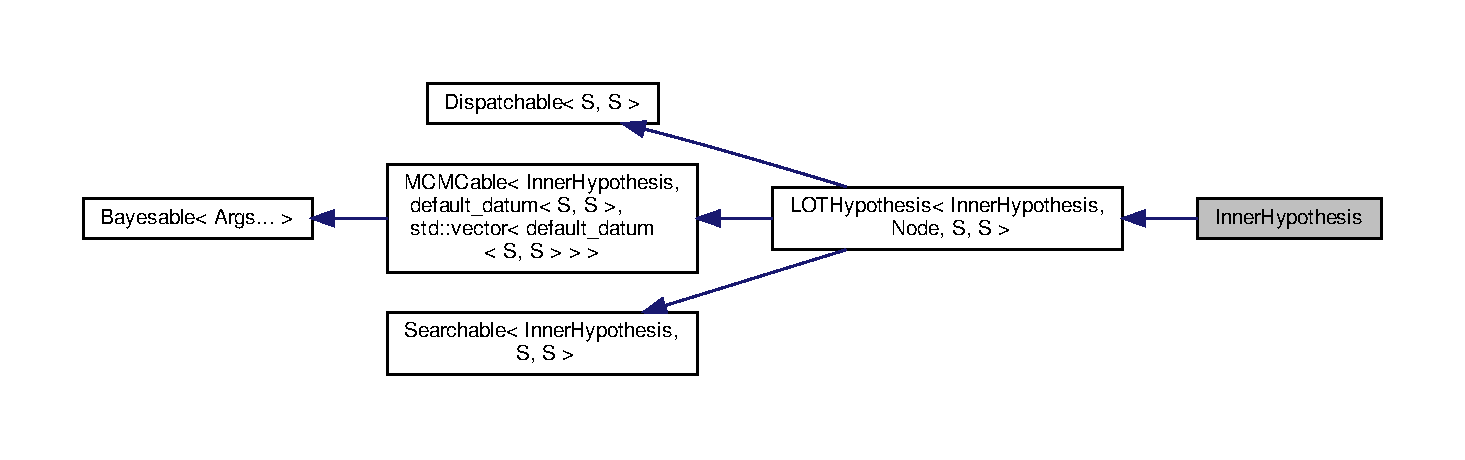
\includegraphics[width=350pt]{class_inner_hypothesis__inherit__graph}
\end{center}
\end{figure}


Collaboration diagram for Inner\+Hypothesis\+:\nopagebreak
\begin{figure}[H]
\begin{center}
\leavevmode
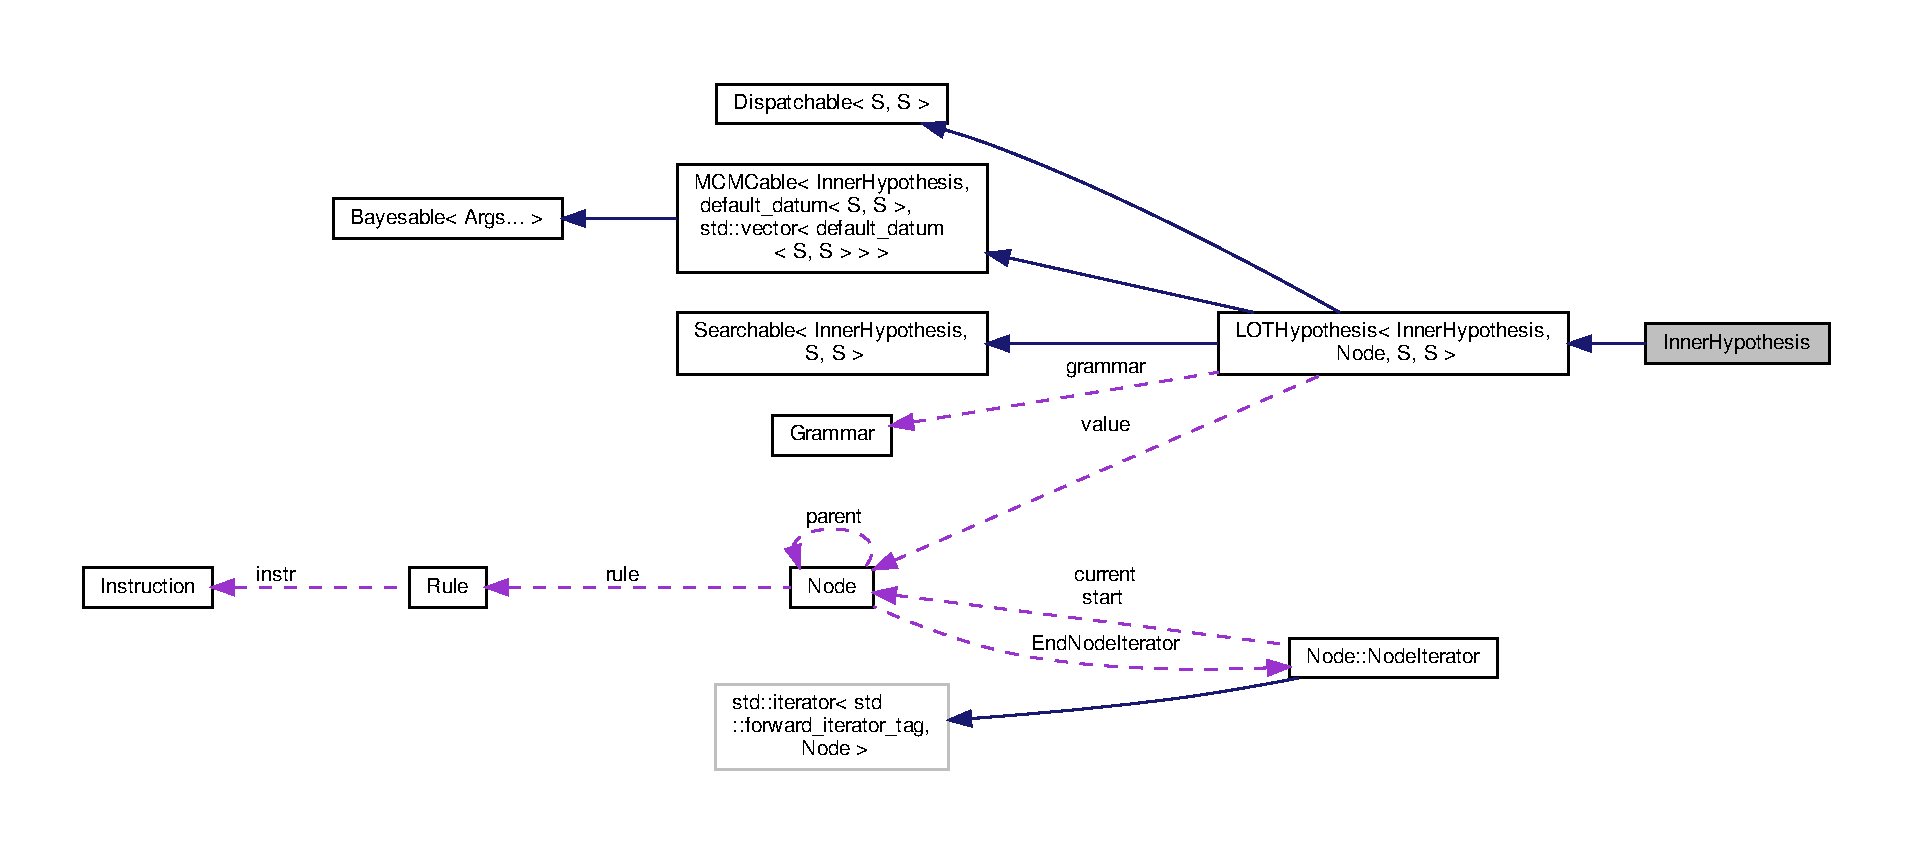
\includegraphics[width=350pt]{class_inner_hypothesis__coll__graph}
\end{center}
\end{figure}
\subsection*{Public Types}
\begin{DoxyCompactItemize}
\item 
using \hyperlink{class_inner_hypothesis_a2c15665b923d905f1f7441282780abc2}{Super} = \hyperlink{class_l_o_t_hypothesis}{L\+O\+T\+Hypothesis}$<$ \hyperlink{class_inner_hypothesis}{Inner\+Hypothesis}, \hyperlink{class_node}{Node}, \hyperlink{_formal_language_theory-_complex_2_main_8cpp_a51c40915539205f0b5add30b0d68a4cb}{S}, \hyperlink{_formal_language_theory-_complex_2_main_8cpp_a51c40915539205f0b5add30b0d68a4cb}{S} $>$
\end{DoxyCompactItemize}
\subsection*{Public Member Functions}
\begin{DoxyCompactItemize}
\item 
virtual \hyperlink{_instruction_8h_a6202215407ab29590bb936ca2996cf64}{vmstatus\+\_\+t} \hyperlink{class_inner_hypothesis_a9aea852725a3798aafeae5e7a5a0736b}{dispatch\+\_\+custom} (\hyperlink{class_instruction}{Instruction} i, \hyperlink{class_virtual_machine_pool}{Virtual\+Machine\+Pool}$<$ \hyperlink{_formal_language_theory-_complex_2_main_8cpp_a51c40915539205f0b5add30b0d68a4cb}{S}, \hyperlink{_formal_language_theory-_complex_2_main_8cpp_a51c40915539205f0b5add30b0d68a4cb}{S} $>$ $\ast$pool, \hyperlink{class_virtual_machine_state}{Virtual\+Machine\+State}$<$ \hyperlink{_formal_language_theory-_complex_2_main_8cpp_a51c40915539205f0b5add30b0d68a4cb}{S}, \hyperlink{_formal_language_theory-_complex_2_main_8cpp_a51c40915539205f0b5add30b0d68a4cb}{S} $>$ $\ast$vms, \hyperlink{class_dispatchable}{Dispatchable}$<$ \hyperlink{_formal_language_theory-_complex_2_main_8cpp_a51c40915539205f0b5add30b0d68a4cb}{S}, \hyperlink{_formal_language_theory-_complex_2_main_8cpp_a51c40915539205f0b5add30b0d68a4cb}{S} $>$ $\ast$loader)
\end{DoxyCompactItemize}
\subsection*{Additional Inherited Members}


\subsection{Member Typedef Documentation}
\mbox{\Hypertarget{class_inner_hypothesis_a2c15665b923d905f1f7441282780abc2}\label{class_inner_hypothesis_a2c15665b923d905f1f7441282780abc2}} 
\index{Inner\+Hypothesis@{Inner\+Hypothesis}!Super@{Super}}
\index{Super@{Super}!Inner\+Hypothesis@{Inner\+Hypothesis}}
\subsubsection{\texorpdfstring{Super}{Super}}
{\footnotesize\ttfamily using \hyperlink{class_inner_hypothesis_a2c15665b923d905f1f7441282780abc2}{Inner\+Hypothesis\+::\+Super} =  \hyperlink{class_l_o_t_hypothesis}{L\+O\+T\+Hypothesis}$<$\hyperlink{class_inner_hypothesis}{Inner\+Hypothesis},\hyperlink{class_node}{Node},\hyperlink{_formal_language_theory-_complex_2_main_8cpp_a51c40915539205f0b5add30b0d68a4cb}{S},\hyperlink{_formal_language_theory-_complex_2_main_8cpp_a51c40915539205f0b5add30b0d68a4cb}{S}$>$}



\subsection{Member Function Documentation}
\mbox{\Hypertarget{class_inner_hypothesis_a9aea852725a3798aafeae5e7a5a0736b}\label{class_inner_hypothesis_a9aea852725a3798aafeae5e7a5a0736b}} 
\index{Inner\+Hypothesis@{Inner\+Hypothesis}!dispatch\+\_\+custom@{dispatch\+\_\+custom}}
\index{dispatch\+\_\+custom@{dispatch\+\_\+custom}!Inner\+Hypothesis@{Inner\+Hypothesis}}
\subsubsection{\texorpdfstring{dispatch\+\_\+custom()}{dispatch\_custom()}}
{\footnotesize\ttfamily virtual \hyperlink{_instruction_8h_a6202215407ab29590bb936ca2996cf64}{vmstatus\+\_\+t} Inner\+Hypothesis\+::dispatch\+\_\+custom (\begin{DoxyParamCaption}\item[{\hyperlink{class_instruction}{Instruction}}]{i,  }\item[{\hyperlink{class_virtual_machine_pool}{Virtual\+Machine\+Pool}$<$ \hyperlink{_formal_language_theory-_complex_2_main_8cpp_a51c40915539205f0b5add30b0d68a4cb}{S}, \hyperlink{_formal_language_theory-_complex_2_main_8cpp_a51c40915539205f0b5add30b0d68a4cb}{S} $>$ $\ast$}]{pool,  }\item[{\hyperlink{class_virtual_machine_state}{Virtual\+Machine\+State}$<$ \hyperlink{_formal_language_theory-_complex_2_main_8cpp_a51c40915539205f0b5add30b0d68a4cb}{S}, \hyperlink{_formal_language_theory-_complex_2_main_8cpp_a51c40915539205f0b5add30b0d68a4cb}{S} $>$ $\ast$}]{vms,  }\item[{\hyperlink{class_dispatchable}{Dispatchable}$<$ \hyperlink{_formal_language_theory-_complex_2_main_8cpp_a51c40915539205f0b5add30b0d68a4cb}{S}, \hyperlink{_formal_language_theory-_complex_2_main_8cpp_a51c40915539205f0b5add30b0d68a4cb}{S} $>$ $\ast$}]{loader }\end{DoxyParamCaption})\hspace{0.3cm}{\ttfamily [inline]}, {\ttfamily [virtual]}}



Reimplemented from \hyperlink{class_l_o_t_hypothesis_a6eae1ce4486971909e0245ab9e30ddeb}{L\+O\+T\+Hypothesis$<$ Inner\+Hypothesis, Node, S, S $>$}.



The documentation for this class was generated from the following file\+:\begin{DoxyCompactItemize}
\item 
Models/\+Formal\+Language\+Theory-\/\+Complex/\hyperlink{_formal_language_theory-_complex_2_main_8cpp}{Main.\+cpp}\end{DoxyCompactItemize}

\hypertarget{class_instruction}{}\section{Instruction Class Reference}
\label{class_instruction}\index{Instruction@{Instruction}}


{\ttfamily \#include $<$Instruction.\+h$>$}

\subsection*{Public Member Functions}
\begin{DoxyCompactItemize}
\item 
\hyperlink{class_instruction_aebd15229c1651af49dcb203707e7a2d5}{Instruction} ()
\item 
\hyperlink{class_instruction_a7f672d88ba4ec174716bbac9adb8b1b0}{Instruction} (\hyperlink{_instruction_8h_af2fb7c87c5854c5733d7bb0506b06de7}{Builtin\+Op} x, int arg\+\_\+=0x0)
\item 
\hyperlink{class_instruction_afbd8f0bdce88feee59e23abf82c8a718}{Instruction} (\hyperlink{_instruction_8h_a3a20ca4a8f0ab220518b030cc23ffee4}{Custom\+Op} x, int arg\+\_\+=0x0)
\item 
\hyperlink{class_instruction_a62d7782f809fa55635a6ced1e971eb3b}{Instruction} (\hyperlink{_instruction_8h_a227278394efd1e2313c727102db09ea9}{Primitive\+Op} x, int arg\+\_\+=0x0)
\item 
{\footnotesize template$<$typename t $>$ }\\bool \hyperlink{class_instruction_ade73e12471250fd191362d462e2f4970}{is} () const
\item 
{\footnotesize template$<$typename t $>$ }\\t \hyperlink{class_instruction_ac99272000afeb9015a9d40ceed8c139b}{as} () const
\item 
int \hyperlink{class_instruction_a83a2763aa1dab5281b27dd99925f683e}{get\+Arg} () const
\item 
bool \hyperlink{class_instruction_a75e0ecee9ec917bcc47488a1fbeb6a24}{operator==} (const \hyperlink{class_instruction}{Instruction} \&i) const
\item 
{\footnotesize template$<$typename T $>$ }\\bool \hyperlink{class_instruction_a924203cd9a0516d64556ecbf6a79df8a}{is\+\_\+a} (const T x) const
\begin{DoxyCompactList}\small\item\em compare the instruction types (ignores the arg) \end{DoxyCompactList}\item 
{\footnotesize template$<$typename T , typename... Ts$>$ }\\bool \hyperlink{class_instruction_ae670ee58f9acdfd60b7213f77dfca794}{is\+\_\+a} (T x, Ts... args) const
\end{DoxyCompactItemize}
\subsection*{Public Attributes}
\begin{DoxyCompactItemize}
\item 
std\+::variant$<$ \hyperlink{_instruction_8h_af2fb7c87c5854c5733d7bb0506b06de7}{Builtin\+Op}, \hyperlink{_instruction_8h_a3a20ca4a8f0ab220518b030cc23ffee4}{Custom\+Op}, \hyperlink{_instruction_8h_a227278394efd1e2313c727102db09ea9}{Primitive\+Op} $>$ \hyperlink{class_instruction_ace2bace7950c18f67d1568fb56e9e6de}{op}
\item 
int \hyperlink{class_instruction_a7ed399e29ec58e97a7b6311919f5d5ca}{arg}
\end{DoxyCompactItemize}


\subsection{Detailed Description}
\begin{DoxyAuthor}{Author}
piantado 
\end{DoxyAuthor}
\begin{DoxyDate}{Date}
29/01/20 
\end{DoxyDate}


\subsection{Constructor \& Destructor Documentation}
\mbox{\Hypertarget{class_instruction_aebd15229c1651af49dcb203707e7a2d5}\label{class_instruction_aebd15229c1651af49dcb203707e7a2d5}} 
\index{Instruction@{Instruction}!Instruction@{Instruction}}
\index{Instruction@{Instruction}!Instruction@{Instruction}}
\subsubsection{\texorpdfstring{Instruction()}{Instruction()}\hspace{0.1cm}{\footnotesize\ttfamily [1/4]}}
{\footnotesize\ttfamily Instruction\+::\+Instruction (\begin{DoxyParamCaption}{ }\end{DoxyParamCaption})\hspace{0.3cm}{\ttfamily [inline]}}

\mbox{\Hypertarget{class_instruction_a7f672d88ba4ec174716bbac9adb8b1b0}\label{class_instruction_a7f672d88ba4ec174716bbac9adb8b1b0}} 
\index{Instruction@{Instruction}!Instruction@{Instruction}}
\index{Instruction@{Instruction}!Instruction@{Instruction}}
\subsubsection{\texorpdfstring{Instruction()}{Instruction()}\hspace{0.1cm}{\footnotesize\ttfamily [2/4]}}
{\footnotesize\ttfamily Instruction\+::\+Instruction (\begin{DoxyParamCaption}\item[{\hyperlink{_instruction_8h_af2fb7c87c5854c5733d7bb0506b06de7}{Builtin\+Op}}]{x,  }\item[{int}]{arg\+\_\+ = {\ttfamily 0x0} }\end{DoxyParamCaption})\hspace{0.3cm}{\ttfamily [inline]}}

\mbox{\Hypertarget{class_instruction_afbd8f0bdce88feee59e23abf82c8a718}\label{class_instruction_afbd8f0bdce88feee59e23abf82c8a718}} 
\index{Instruction@{Instruction}!Instruction@{Instruction}}
\index{Instruction@{Instruction}!Instruction@{Instruction}}
\subsubsection{\texorpdfstring{Instruction()}{Instruction()}\hspace{0.1cm}{\footnotesize\ttfamily [3/4]}}
{\footnotesize\ttfamily Instruction\+::\+Instruction (\begin{DoxyParamCaption}\item[{\hyperlink{_instruction_8h_a3a20ca4a8f0ab220518b030cc23ffee4}{Custom\+Op}}]{x,  }\item[{int}]{arg\+\_\+ = {\ttfamily 0x0} }\end{DoxyParamCaption})\hspace{0.3cm}{\ttfamily [inline]}}

\mbox{\Hypertarget{class_instruction_a62d7782f809fa55635a6ced1e971eb3b}\label{class_instruction_a62d7782f809fa55635a6ced1e971eb3b}} 
\index{Instruction@{Instruction}!Instruction@{Instruction}}
\index{Instruction@{Instruction}!Instruction@{Instruction}}
\subsubsection{\texorpdfstring{Instruction()}{Instruction()}\hspace{0.1cm}{\footnotesize\ttfamily [4/4]}}
{\footnotesize\ttfamily Instruction\+::\+Instruction (\begin{DoxyParamCaption}\item[{\hyperlink{_instruction_8h_a227278394efd1e2313c727102db09ea9}{Primitive\+Op}}]{x,  }\item[{int}]{arg\+\_\+ = {\ttfamily 0x0} }\end{DoxyParamCaption})\hspace{0.3cm}{\ttfamily [inline]}}



\subsection{Member Function Documentation}
\mbox{\Hypertarget{class_instruction_ac99272000afeb9015a9d40ceed8c139b}\label{class_instruction_ac99272000afeb9015a9d40ceed8c139b}} 
\index{Instruction@{Instruction}!as@{as}}
\index{as@{as}!Instruction@{Instruction}}
\subsubsection{\texorpdfstring{as()}{as()}}
{\footnotesize\ttfamily template$<$typename t $>$ \\
t Instruction\+::as (\begin{DoxyParamCaption}{ }\end{DoxyParamCaption}) const\hspace{0.3cm}{\ttfamily [inline]}}

Get as type t \begin{DoxyReturn}{Returns}

\end{DoxyReturn}
\mbox{\Hypertarget{class_instruction_a83a2763aa1dab5281b27dd99925f683e}\label{class_instruction_a83a2763aa1dab5281b27dd99925f683e}} 
\index{Instruction@{Instruction}!get\+Arg@{get\+Arg}}
\index{get\+Arg@{get\+Arg}!Instruction@{Instruction}}
\subsubsection{\texorpdfstring{get\+Arg()}{getArg()}}
{\footnotesize\ttfamily int Instruction\+::get\+Arg (\begin{DoxyParamCaption}{ }\end{DoxyParamCaption}) const\hspace{0.3cm}{\ttfamily [inline]}}

Return the argument (an int) \begin{DoxyReturn}{Returns}

\end{DoxyReturn}
\mbox{\Hypertarget{class_instruction_ade73e12471250fd191362d462e2f4970}\label{class_instruction_ade73e12471250fd191362d462e2f4970}} 
\index{Instruction@{Instruction}!is@{is}}
\index{is@{is}!Instruction@{Instruction}}
\subsubsection{\texorpdfstring{is()}{is()}}
{\footnotesize\ttfamily template$<$typename t $>$ \\
bool Instruction\+::is (\begin{DoxyParamCaption}{ }\end{DoxyParamCaption}) const\hspace{0.3cm}{\ttfamily [inline]}}

Template to check if this instruction is holding type t \begin{DoxyReturn}{Returns}

\end{DoxyReturn}
\mbox{\Hypertarget{class_instruction_a924203cd9a0516d64556ecbf6a79df8a}\label{class_instruction_a924203cd9a0516d64556ecbf6a79df8a}} 
\index{Instruction@{Instruction}!is\+\_\+a@{is\+\_\+a}}
\index{is\+\_\+a@{is\+\_\+a}!Instruction@{Instruction}}
\subsubsection{\texorpdfstring{is\+\_\+a()}{is\_a()}\hspace{0.1cm}{\footnotesize\ttfamily [1/2]}}
{\footnotesize\ttfamily template$<$typename T $>$ \\
bool Instruction\+::is\+\_\+a (\begin{DoxyParamCaption}\item[{const T}]{x }\end{DoxyParamCaption}) const\hspace{0.3cm}{\ttfamily [inline]}}



compare the instruction types (ignores the arg) 

\mbox{\Hypertarget{class_instruction_ae670ee58f9acdfd60b7213f77dfca794}\label{class_instruction_ae670ee58f9acdfd60b7213f77dfca794}} 
\index{Instruction@{Instruction}!is\+\_\+a@{is\+\_\+a}}
\index{is\+\_\+a@{is\+\_\+a}!Instruction@{Instruction}}
\subsubsection{\texorpdfstring{is\+\_\+a()}{is\_a()}\hspace{0.1cm}{\footnotesize\ttfamily [2/2]}}
{\footnotesize\ttfamily template$<$typename T , typename... Ts$>$ \\
bool Instruction\+::is\+\_\+a (\begin{DoxyParamCaption}\item[{T}]{x,  }\item[{Ts...}]{args }\end{DoxyParamCaption}) const\hspace{0.3cm}{\ttfamily [inline]}}

Variadic checking of whether this is a given op type 
\begin{DoxyParams}{Parameters}
{\em x} & \\
\hline
\end{DoxyParams}
\begin{DoxyReturn}{Returns}

\end{DoxyReturn}
\mbox{\Hypertarget{class_instruction_a75e0ecee9ec917bcc47488a1fbeb6a24}\label{class_instruction_a75e0ecee9ec917bcc47488a1fbeb6a24}} 
\index{Instruction@{Instruction}!operator==@{operator==}}
\index{operator==@{operator==}!Instruction@{Instruction}}
\subsubsection{\texorpdfstring{operator==()}{operator==()}}
{\footnotesize\ttfamily bool Instruction\+::operator== (\begin{DoxyParamCaption}\item[{const \hyperlink{class_instruction}{Instruction} \&}]{i }\end{DoxyParamCaption}) const\hspace{0.3cm}{\ttfamily [inline]}}



\subsection{Member Data Documentation}
\mbox{\Hypertarget{class_instruction_a7ed399e29ec58e97a7b6311919f5d5ca}\label{class_instruction_a7ed399e29ec58e97a7b6311919f5d5ca}} 
\index{Instruction@{Instruction}!arg@{arg}}
\index{arg@{arg}!Instruction@{Instruction}}
\subsubsection{\texorpdfstring{arg}{arg}}
{\footnotesize\ttfamily int Instruction\+::arg}

\mbox{\Hypertarget{class_instruction_ace2bace7950c18f67d1568fb56e9e6de}\label{class_instruction_ace2bace7950c18f67d1568fb56e9e6de}} 
\index{Instruction@{Instruction}!op@{op}}
\index{op@{op}!Instruction@{Instruction}}
\subsubsection{\texorpdfstring{op}{op}}
{\footnotesize\ttfamily std\+::variant$<$\hyperlink{_instruction_8h_af2fb7c87c5854c5733d7bb0506b06de7}{Builtin\+Op}, \hyperlink{_instruction_8h_a3a20ca4a8f0ab220518b030cc23ffee4}{Custom\+Op}, \hyperlink{_instruction_8h_a227278394efd1e2313c727102db09ea9}{Primitive\+Op}$>$ Instruction\+::op}



The documentation for this class was generated from the following file\+:\begin{DoxyCompactItemize}
\item 
src/\+Virtual\+Machine/\hyperlink{_instruction_8h}{Instruction.\+h}\end{DoxyCompactItemize}

\hypertarget{class_integerized_stack}{}\section{Integerized\+Stack Class Reference}
\label{class_integerized_stack}\index{Integerized\+Stack@{Integerized\+Stack}}


{\ttfamily \#include $<$Integerized\+Stack.\+h$>$}

\subsection*{Public Member Functions}
\begin{DoxyCompactItemize}
\item 
\hyperlink{class_integerized_stack_a46b24ace7ea983bfabaa437932111440}{Integerized\+Stack} (value\+\_\+t v=0)
\item 
value\+\_\+t \hyperlink{class_integerized_stack_a5edd593c74341341cc6f8e41e0f14bdf}{pop} ()
\item 
value\+\_\+t \hyperlink{class_integerized_stack_a713da8c8102cb5a53ec3ad87fada36f5}{pop} (value\+\_\+t modulus)
\item 
void \hyperlink{class_integerized_stack_a721481e52e56398bee39edf6a3d2ff80}{push} (value\+\_\+t x)
\item 
void \hyperlink{class_integerized_stack_affd28eb928362de80e35cd4e1ecdf96b}{push} (value\+\_\+t x, value\+\_\+t modulus)
\item 
value\+\_\+t \hyperlink{class_integerized_stack_ac72013ff1034d8f05470e8314cf8525d}{get\+\_\+value} ()
\item 
bool \hyperlink{class_integerized_stack_a549d4ed66e89d2e3d7e726d5c8e28fa2}{empty} () const
\item 
void \hyperlink{class_integerized_stack_a829e18dc8bae3eb371e9822271102a2d}{operator=} (value\+\_\+t z)
\item 
void \hyperlink{class_integerized_stack_ac2ec311399b327573a2c0f19d2a902a4}{operator-\/=} (value\+\_\+t x)
\item 
void \hyperlink{class_integerized_stack_a70df05b936e94c717584290d0c457cca}{operator+=} (value\+\_\+t x)
\end{DoxyCompactItemize}
\subsection*{Protected Attributes}
\begin{DoxyCompactItemize}
\item 
value\+\_\+t \hyperlink{class_integerized_stack_afcfb2d32d51c88b556f3bb7ff2544be5}{value}
\end{DoxyCompactItemize}


\subsection{Constructor \& Destructor Documentation}
\mbox{\Hypertarget{class_integerized_stack_a46b24ace7ea983bfabaa437932111440}\label{class_integerized_stack_a46b24ace7ea983bfabaa437932111440}} 
\index{Integerized\+Stack@{Integerized\+Stack}!Integerized\+Stack@{Integerized\+Stack}}
\index{Integerized\+Stack@{Integerized\+Stack}!Integerized\+Stack@{Integerized\+Stack}}
\subsubsection{\texorpdfstring{Integerized\+Stack()}{IntegerizedStack()}}
{\footnotesize\ttfamily Integerized\+Stack\+::\+Integerized\+Stack (\begin{DoxyParamCaption}\item[{value\+\_\+t}]{v = {\ttfamily 0} }\end{DoxyParamCaption})\hspace{0.3cm}{\ttfamily [inline]}}



\subsection{Member Function Documentation}
\mbox{\Hypertarget{class_integerized_stack_a549d4ed66e89d2e3d7e726d5c8e28fa2}\label{class_integerized_stack_a549d4ed66e89d2e3d7e726d5c8e28fa2}} 
\index{Integerized\+Stack@{Integerized\+Stack}!empty@{empty}}
\index{empty@{empty}!Integerized\+Stack@{Integerized\+Stack}}
\subsubsection{\texorpdfstring{empty()}{empty()}}
{\footnotesize\ttfamily bool Integerized\+Stack\+::empty (\begin{DoxyParamCaption}{ }\end{DoxyParamCaption}) const\hspace{0.3cm}{\ttfamily [inline]}}

\mbox{\Hypertarget{class_integerized_stack_ac72013ff1034d8f05470e8314cf8525d}\label{class_integerized_stack_ac72013ff1034d8f05470e8314cf8525d}} 
\index{Integerized\+Stack@{Integerized\+Stack}!get\+\_\+value@{get\+\_\+value}}
\index{get\+\_\+value@{get\+\_\+value}!Integerized\+Stack@{Integerized\+Stack}}
\subsubsection{\texorpdfstring{get\+\_\+value()}{get\_value()}}
{\footnotesize\ttfamily value\+\_\+t Integerized\+Stack\+::get\+\_\+value (\begin{DoxyParamCaption}{ }\end{DoxyParamCaption})\hspace{0.3cm}{\ttfamily [inline]}}

\mbox{\Hypertarget{class_integerized_stack_a70df05b936e94c717584290d0c457cca}\label{class_integerized_stack_a70df05b936e94c717584290d0c457cca}} 
\index{Integerized\+Stack@{Integerized\+Stack}!operator+=@{operator+=}}
\index{operator+=@{operator+=}!Integerized\+Stack@{Integerized\+Stack}}
\subsubsection{\texorpdfstring{operator+=()}{operator+=()}}
{\footnotesize\ttfamily void Integerized\+Stack\+::operator+= (\begin{DoxyParamCaption}\item[{value\+\_\+t}]{x }\end{DoxyParamCaption})\hspace{0.3cm}{\ttfamily [inline]}}

\mbox{\Hypertarget{class_integerized_stack_ac2ec311399b327573a2c0f19d2a902a4}\label{class_integerized_stack_ac2ec311399b327573a2c0f19d2a902a4}} 
\index{Integerized\+Stack@{Integerized\+Stack}!operator-\/=@{operator-\/=}}
\index{operator-\/=@{operator-\/=}!Integerized\+Stack@{Integerized\+Stack}}
\subsubsection{\texorpdfstring{operator-\/=()}{operator-=()}}
{\footnotesize\ttfamily void Integerized\+Stack\+::operator-\/= (\begin{DoxyParamCaption}\item[{value\+\_\+t}]{x }\end{DoxyParamCaption})\hspace{0.3cm}{\ttfamily [inline]}}

\mbox{\Hypertarget{class_integerized_stack_a829e18dc8bae3eb371e9822271102a2d}\label{class_integerized_stack_a829e18dc8bae3eb371e9822271102a2d}} 
\index{Integerized\+Stack@{Integerized\+Stack}!operator=@{operator=}}
\index{operator=@{operator=}!Integerized\+Stack@{Integerized\+Stack}}
\subsubsection{\texorpdfstring{operator=()}{operator=()}}
{\footnotesize\ttfamily void Integerized\+Stack\+::operator= (\begin{DoxyParamCaption}\item[{value\+\_\+t}]{z }\end{DoxyParamCaption})\hspace{0.3cm}{\ttfamily [inline]}}

\mbox{\Hypertarget{class_integerized_stack_a5edd593c74341341cc6f8e41e0f14bdf}\label{class_integerized_stack_a5edd593c74341341cc6f8e41e0f14bdf}} 
\index{Integerized\+Stack@{Integerized\+Stack}!pop@{pop}}
\index{pop@{pop}!Integerized\+Stack@{Integerized\+Stack}}
\subsubsection{\texorpdfstring{pop()}{pop()}\hspace{0.1cm}{\footnotesize\ttfamily [1/2]}}
{\footnotesize\ttfamily value\+\_\+t Integerized\+Stack\+::pop (\begin{DoxyParamCaption}{ }\end{DoxyParamCaption})\hspace{0.3cm}{\ttfamily [inline]}}

\mbox{\Hypertarget{class_integerized_stack_a713da8c8102cb5a53ec3ad87fada36f5}\label{class_integerized_stack_a713da8c8102cb5a53ec3ad87fada36f5}} 
\index{Integerized\+Stack@{Integerized\+Stack}!pop@{pop}}
\index{pop@{pop}!Integerized\+Stack@{Integerized\+Stack}}
\subsubsection{\texorpdfstring{pop()}{pop()}\hspace{0.1cm}{\footnotesize\ttfamily [2/2]}}
{\footnotesize\ttfamily value\+\_\+t Integerized\+Stack\+::pop (\begin{DoxyParamCaption}\item[{value\+\_\+t}]{modulus }\end{DoxyParamCaption})\hspace{0.3cm}{\ttfamily [inline]}}

\mbox{\Hypertarget{class_integerized_stack_a721481e52e56398bee39edf6a3d2ff80}\label{class_integerized_stack_a721481e52e56398bee39edf6a3d2ff80}} 
\index{Integerized\+Stack@{Integerized\+Stack}!push@{push}}
\index{push@{push}!Integerized\+Stack@{Integerized\+Stack}}
\subsubsection{\texorpdfstring{push()}{push()}\hspace{0.1cm}{\footnotesize\ttfamily [1/2]}}
{\footnotesize\ttfamily void Integerized\+Stack\+::push (\begin{DoxyParamCaption}\item[{value\+\_\+t}]{x }\end{DoxyParamCaption})\hspace{0.3cm}{\ttfamily [inline]}}

\mbox{\Hypertarget{class_integerized_stack_affd28eb928362de80e35cd4e1ecdf96b}\label{class_integerized_stack_affd28eb928362de80e35cd4e1ecdf96b}} 
\index{Integerized\+Stack@{Integerized\+Stack}!push@{push}}
\index{push@{push}!Integerized\+Stack@{Integerized\+Stack}}
\subsubsection{\texorpdfstring{push()}{push()}\hspace{0.1cm}{\footnotesize\ttfamily [2/2]}}
{\footnotesize\ttfamily void Integerized\+Stack\+::push (\begin{DoxyParamCaption}\item[{value\+\_\+t}]{x,  }\item[{value\+\_\+t}]{modulus }\end{DoxyParamCaption})\hspace{0.3cm}{\ttfamily [inline]}}



\subsection{Member Data Documentation}
\mbox{\Hypertarget{class_integerized_stack_afcfb2d32d51c88b556f3bb7ff2544be5}\label{class_integerized_stack_afcfb2d32d51c88b556f3bb7ff2544be5}} 
\index{Integerized\+Stack@{Integerized\+Stack}!value@{value}}
\index{value@{value}!Integerized\+Stack@{Integerized\+Stack}}
\subsubsection{\texorpdfstring{value}{value}}
{\footnotesize\ttfamily value\+\_\+t Integerized\+Stack\+::value\hspace{0.3cm}{\ttfamily [protected]}}



The documentation for this class was generated from the following file\+:\begin{DoxyCompactItemize}
\item 
src/\hyperlink{_integerized_stack_8h}{Integerized\+Stack.\+h}\end{DoxyCompactItemize}

\hypertarget{structis__iterable}{}\section{is\+\_\+iterable$<$ T, typename $>$ Struct Template Reference}
\label{structis__iterable}\index{is\+\_\+iterable$<$ T, typename $>$@{is\+\_\+iterable$<$ T, typename $>$}}


Converts our own time format to ms, which is what \hyperlink{namespace_fleet}{Fleet}\textquotesingle{}s time utilities use The time format we accept is \#+(.\#+)\mbox{[}smhd\mbox{]} where shmd specifies seconds, minutes, hours days.  




{\ttfamily \#include $<$Miscellaneous.\+h$>$}



Inheritance diagram for is\+\_\+iterable$<$ T, typename $>$\+:\nopagebreak
\begin{figure}[H]
\begin{center}
\leavevmode
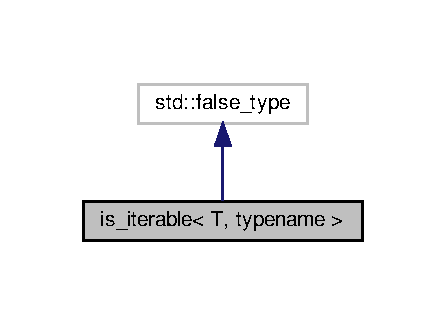
\includegraphics[width=214pt]{structis__iterable__inherit__graph}
\end{center}
\end{figure}


Collaboration diagram for is\+\_\+iterable$<$ T, typename $>$\+:\nopagebreak
\begin{figure}[H]
\begin{center}
\leavevmode
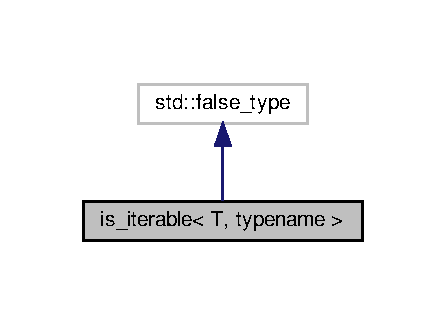
\includegraphics[width=214pt]{structis__iterable__coll__graph}
\end{center}
\end{figure}


\subsection{Detailed Description}
\subsubsection*{template$<$typename T, typename = void$>$\newline
struct is\+\_\+iterable$<$ T, typename $>$}

Converts our own time format to ms, which is what \hyperlink{namespace_fleet}{Fleet}\textquotesingle{}s time utilities use The time format we accept is \#+(.\#+)\mbox{[}smhd\mbox{]} where shmd specifies seconds, minutes, hours days. 


\begin{DoxyCode}
    Time conversions \textcolor{keywordflow}{for} fleet
   ~~~~~~~~~~~~~~~~~~~~~~~~~~~~~~~~~~~~~~~~~~~~~~~~~~~~~~~~~~~~~~~~~~~~~~~~~~~~~~~~~~~~~~~~ */

time\_t convert\_time(std::string& s) \{
    \textcolor{comment}{// specila case of s="0" will be allowed}
    \textcolor{keywordflow}{if}(s == \textcolor{stringliteral}{"0"}) \textcolor{keywordflow}{return} 0;

    \textcolor{comment}{// else we must specify a unit  }
    \textcolor{keywordtype}{double} multiplier; \textcolor{comment}{// for default multiplier of 1 is seconds}
    \textcolor{keywordflow}{switch}(s.at(s.length()-1)) \{
        \textcolor{keywordflow}{case} \textcolor{charliteral}{'s'}: multiplier = 1000; \textcolor{keywordflow}{break}; 
        \textcolor{keywordflow}{case} \textcolor{charliteral}{'m'}: multiplier = 60*1000; \textcolor{keywordflow}{break};
        \textcolor{keywordflow}{case} \textcolor{charliteral}{'h'}: multiplier = 60*60*1000; \textcolor{keywordflow}{break};
        \textcolor{keywordflow}{case} \textcolor{charliteral}{'d'}: multiplier = 60*60*24*1000; \textcolor{keywordflow}{break};
        \textcolor{keywordflow}{default}: 
            \hyperlink{_i_o_8h_a176c0577baa96c686397bca42f7ee6ff}{CERR} \textcolor{stringliteral}{"*** Unknown time specifier: "} << s.at(s.length()-1) << \textcolor{stringliteral}{" in "} << s << \textcolor{stringliteral}{". Did you
       forget a unit?"} \hyperlink{_i_o_8h_a90dc3f3ee970394e0080300526390a84}{ENDL};
            assert(0);
    \}

    \textcolor{keywordtype}{double} t = std::stod(s.substr(0,s.length()-1)); \textcolor{comment}{// all but the last character}

    \textcolor{keywordflow}{return} (\textcolor{keywordtype}{unsigned} \textcolor{keywordtype}{long})(t*multiplier); \textcolor{comment}{// note this effectively rounds to the nearest second }

\}

\textcolor{comment}{// Python-like pass statements}
\textcolor{preprocessor}{#define pass}


\textcolor{comment}{/*}
\end{DoxyCode}
 Template magic to check if a class is iterable $\sim$$\sim$$\sim$$\sim$$\sim$$\sim$$\sim$$\sim$$\sim$$\sim$$\sim$$\sim$$\sim$$\sim$$\sim$$\sim$$\sim$$\sim$$\sim$$\sim$$\sim$$\sim$$\sim$$\sim$$\sim$$\sim$$\sim$$\sim$$\sim$$\sim$$\sim$$\sim$$\sim$$\sim$$\sim$$\sim$$\sim$$\sim$$\sim$$\sim$$\sim$$\sim$$\sim$$\sim$$\sim$$\sim$$\sim$$\sim$$\sim$$\sim$$\sim$$\sim$$\sim$$\sim$$\sim$$\sim$$\sim$$\sim$$\sim$$\sim$$\sim$$\sim$$\sim$$\sim$$\sim$$\sim$$\sim$$\sim$$\sim$$\sim$$\sim$$\sim$$\sim$$\sim$$\sim$$\sim$$\sim$$\sim$$\sim$$\sim$$\sim$$\sim$$\sim$$\sim$$\sim$$\sim$$\sim$$\sim$ 

The documentation for this struct was generated from the following file\+:\begin{DoxyCompactItemize}
\item 
src/\hyperlink{_miscellaneous_8h}{Miscellaneous.\+h}\end{DoxyCompactItemize}

\hypertarget{structis__iterable_3_01_t_00_01std_1_1void__t_3_01decltype_07std_1_1begin_07std_1_1declval_3_01_6e9fb167ef7cf6be085c68f3355f458c}{}\section{is\+\_\+iterable$<$ T, std\+:\+:void\+\_\+t$<$ decltype(std\+:\+:begin(std\+:\+:declval$<$ T $>$())), decltype(std\+:\+:end(std\+:\+:declval$<$ T $>$())) $>$ $>$ Struct Template Reference}
\label{structis__iterable_3_01_t_00_01std_1_1void__t_3_01decltype_07std_1_1begin_07std_1_1declval_3_01_6e9fb167ef7cf6be085c68f3355f458c}\index{is\+\_\+iterable$<$ T, std\+::void\+\_\+t$<$ decltype(std\+::begin(std\+::declval$<$ T $>$())), decltype(std\+::end(std\+::declval$<$ T $>$())) $>$ $>$@{is\+\_\+iterable$<$ T, std\+::void\+\_\+t$<$ decltype(std\+::begin(std\+::declval$<$ T $>$())), decltype(std\+::end(std\+::declval$<$ T $>$())) $>$ $>$}}


{\ttfamily \#include $<$Miscellaneous.\+h$>$}



Inheritance diagram for is\+\_\+iterable$<$ T, std\+:\+:void\+\_\+t$<$ decltype(std\+:\+:begin(std\+:\+:declval$<$ T $>$())), decltype(std\+:\+:end(std\+:\+:declval$<$ T $>$())) $>$ $>$\+:\nopagebreak
\begin{figure}[H]
\begin{center}
\leavevmode
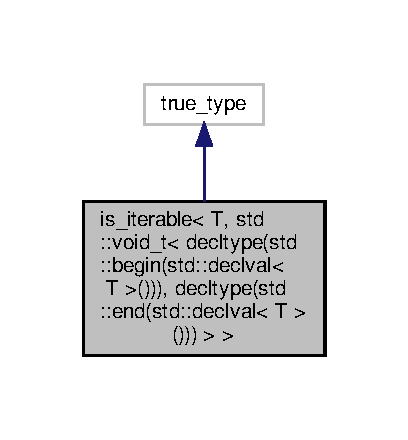
\includegraphics[width=196pt]{structis__iterable_3_01_t_00_01std_1_1void__t_3_01decltype_07std_1_1begin_07std_1_1declval_3_01_b7a4ab461bf675bfc11c691a48b8d31c}
\end{center}
\end{figure}


Collaboration diagram for is\+\_\+iterable$<$ T, std\+:\+:void\+\_\+t$<$ decltype(std\+:\+:begin(std\+:\+:declval$<$ T $>$())), decltype(std\+:\+:end(std\+:\+:declval$<$ T $>$())) $>$ $>$\+:\nopagebreak
\begin{figure}[H]
\begin{center}
\leavevmode
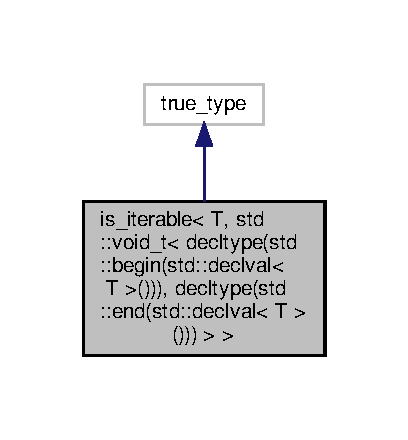
\includegraphics[width=196pt]{structis__iterable_3_01_t_00_01std_1_1void__t_3_01decltype_07std_1_1begin_07std_1_1declval_3_01_b067d8048764f6340460e1309cc193bd}
\end{center}
\end{figure}


The documentation for this struct was generated from the following file\+:\begin{DoxyCompactItemize}
\item 
src/\hyperlink{_miscellaneous_8h}{Miscellaneous.\+h}\end{DoxyCompactItemize}

\hypertarget{class_fleet_1_1_statistics_1_1_reservoir_sample_1_1_item}{}\section{Fleet\+:\+:Statistics\+:\+:Reservoir\+Sample$<$ T $>$\+:\+:Item Class Reference}
\label{class_fleet_1_1_statistics_1_1_reservoir_sample_1_1_item}\index{Fleet\+::\+Statistics\+::\+Reservoir\+Sample$<$ T $>$\+::\+Item@{Fleet\+::\+Statistics\+::\+Reservoir\+Sample$<$ T $>$\+::\+Item}}


{\ttfamily \#include $<$Reservoir\+Sample.\+h$>$}



Collaboration diagram for Fleet\+:\+:Statistics\+:\+:Reservoir\+Sample$<$ T $>$\+:\+:Item\+:\nopagebreak
\begin{figure}[H]
\begin{center}
\leavevmode
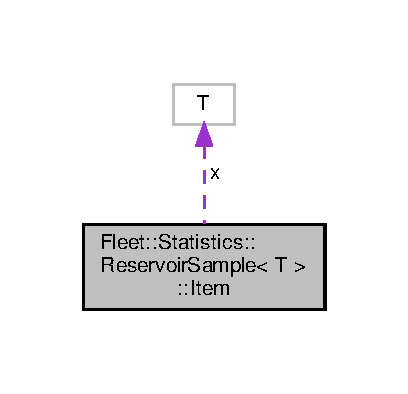
\includegraphics[width=196pt]{class_fleet_1_1_statistics_1_1_reservoir_sample_1_1_item__coll__graph}
\end{center}
\end{figure}
\subsection*{Public Member Functions}
\begin{DoxyCompactItemize}
\item 
\hyperlink{class_fleet_1_1_statistics_1_1_reservoir_sample_1_1_item_acad6abfadffe65005f14a4c9616aabde}{Item} (T x\+\_\+, double r\+\_\+, double lw\+\_\+=0.\+0)
\item 
bool \hyperlink{class_fleet_1_1_statistics_1_1_reservoir_sample_1_1_item_a06bf92e43a3bfe61e75a8bf0d6fa2c67}{operator$<$} (const \hyperlink{class_fleet_1_1_statistics_1_1_reservoir_sample_1_1_item}{Item} \&b) const
\item 
bool \hyperlink{class_fleet_1_1_statistics_1_1_reservoir_sample_1_1_item_ab3adc1f593aec74d7d140f8c3553546e}{operator==} (const \hyperlink{class_fleet_1_1_statistics_1_1_reservoir_sample_1_1_item}{Item} \&b) const
\end{DoxyCompactItemize}
\subsection*{Public Attributes}
\begin{DoxyCompactItemize}
\item 
T \hyperlink{class_fleet_1_1_statistics_1_1_reservoir_sample_1_1_item_ae845a0d698a99e1508241fd25b63dd3a}{x}
\item 
const double \hyperlink{class_fleet_1_1_statistics_1_1_reservoir_sample_1_1_item_a45c460752bf4e0b27ee406d2560479da}{r}
\item 
const double \hyperlink{class_fleet_1_1_statistics_1_1_reservoir_sample_1_1_item_af6e0c0e3569786a8896fcd7ab758a587}{lw}
\item 
const double \hyperlink{class_fleet_1_1_statistics_1_1_reservoir_sample_1_1_item_a0037b193d6712481b90416b51f2eb9d5}{lv}
\end{DoxyCompactItemize}


\subsection{Detailed Description}
\subsubsection*{template$<$typename T$>$\newline
class Fleet\+::\+Statistics\+::\+Reservoir\+Sample$<$ T $>$\+::\+Item}

\begin{DoxyAuthor}{Author}
piantado 
\end{DoxyAuthor}
\begin{DoxyDate}{Date}
29/01/20 
\end{DoxyDate}


\subsection{Constructor \& Destructor Documentation}
\mbox{\Hypertarget{class_fleet_1_1_statistics_1_1_reservoir_sample_1_1_item_acad6abfadffe65005f14a4c9616aabde}\label{class_fleet_1_1_statistics_1_1_reservoir_sample_1_1_item_acad6abfadffe65005f14a4c9616aabde}} 
\index{Fleet\+::\+Statistics\+::\+Reservoir\+Sample\+::\+Item@{Fleet\+::\+Statistics\+::\+Reservoir\+Sample\+::\+Item}!Item@{Item}}
\index{Item@{Item}!Fleet\+::\+Statistics\+::\+Reservoir\+Sample\+::\+Item@{Fleet\+::\+Statistics\+::\+Reservoir\+Sample\+::\+Item}}
\subsubsection{\texorpdfstring{Item()}{Item()}}
{\footnotesize\ttfamily template$<$typename T$>$ \\
\hyperlink{class_fleet_1_1_statistics_1_1_reservoir_sample}{Fleet\+::\+Statistics\+::\+Reservoir\+Sample}$<$ T $>$\+::Item\+::\+Item (\begin{DoxyParamCaption}\item[{T}]{x\+\_\+,  }\item[{double}]{r\+\_\+,  }\item[{double}]{lw\+\_\+ = {\ttfamily 0.0} }\end{DoxyParamCaption})\hspace{0.3cm}{\ttfamily [inline]}}



\subsection{Member Function Documentation}
\mbox{\Hypertarget{class_fleet_1_1_statistics_1_1_reservoir_sample_1_1_item_a06bf92e43a3bfe61e75a8bf0d6fa2c67}\label{class_fleet_1_1_statistics_1_1_reservoir_sample_1_1_item_a06bf92e43a3bfe61e75a8bf0d6fa2c67}} 
\index{Fleet\+::\+Statistics\+::\+Reservoir\+Sample\+::\+Item@{Fleet\+::\+Statistics\+::\+Reservoir\+Sample\+::\+Item}!operator$<$@{operator$<$}}
\index{operator$<$@{operator$<$}!Fleet\+::\+Statistics\+::\+Reservoir\+Sample\+::\+Item@{Fleet\+::\+Statistics\+::\+Reservoir\+Sample\+::\+Item}}
\subsubsection{\texorpdfstring{operator$<$()}{operator<()}}
{\footnotesize\ttfamily template$<$typename T$>$ \\
bool \hyperlink{class_fleet_1_1_statistics_1_1_reservoir_sample}{Fleet\+::\+Statistics\+::\+Reservoir\+Sample}$<$ T $>$\+::Item\+::operator$<$ (\begin{DoxyParamCaption}\item[{const \hyperlink{class_fleet_1_1_statistics_1_1_reservoir_sample_1_1_item}{Item} \&}]{b }\end{DoxyParamCaption}) const\hspace{0.3cm}{\ttfamily [inline]}}

\mbox{\Hypertarget{class_fleet_1_1_statistics_1_1_reservoir_sample_1_1_item_ab3adc1f593aec74d7d140f8c3553546e}\label{class_fleet_1_1_statistics_1_1_reservoir_sample_1_1_item_ab3adc1f593aec74d7d140f8c3553546e}} 
\index{Fleet\+::\+Statistics\+::\+Reservoir\+Sample\+::\+Item@{Fleet\+::\+Statistics\+::\+Reservoir\+Sample\+::\+Item}!operator==@{operator==}}
\index{operator==@{operator==}!Fleet\+::\+Statistics\+::\+Reservoir\+Sample\+::\+Item@{Fleet\+::\+Statistics\+::\+Reservoir\+Sample\+::\+Item}}
\subsubsection{\texorpdfstring{operator==()}{operator==()}}
{\footnotesize\ttfamily template$<$typename T$>$ \\
bool \hyperlink{class_fleet_1_1_statistics_1_1_reservoir_sample}{Fleet\+::\+Statistics\+::\+Reservoir\+Sample}$<$ T $>$\+::Item\+::operator== (\begin{DoxyParamCaption}\item[{const \hyperlink{class_fleet_1_1_statistics_1_1_reservoir_sample_1_1_item}{Item} \&}]{b }\end{DoxyParamCaption}) const\hspace{0.3cm}{\ttfamily [inline]}}



\subsection{Member Data Documentation}
\mbox{\Hypertarget{class_fleet_1_1_statistics_1_1_reservoir_sample_1_1_item_a0037b193d6712481b90416b51f2eb9d5}\label{class_fleet_1_1_statistics_1_1_reservoir_sample_1_1_item_a0037b193d6712481b90416b51f2eb9d5}} 
\index{Fleet\+::\+Statistics\+::\+Reservoir\+Sample\+::\+Item@{Fleet\+::\+Statistics\+::\+Reservoir\+Sample\+::\+Item}!lv@{lv}}
\index{lv@{lv}!Fleet\+::\+Statistics\+::\+Reservoir\+Sample\+::\+Item@{Fleet\+::\+Statistics\+::\+Reservoir\+Sample\+::\+Item}}
\subsubsection{\texorpdfstring{lv}{lv}}
{\footnotesize\ttfamily template$<$typename T$>$ \\
const double \hyperlink{class_fleet_1_1_statistics_1_1_reservoir_sample}{Fleet\+::\+Statistics\+::\+Reservoir\+Sample}$<$ T $>$\+::Item\+::lv}

\mbox{\Hypertarget{class_fleet_1_1_statistics_1_1_reservoir_sample_1_1_item_af6e0c0e3569786a8896fcd7ab758a587}\label{class_fleet_1_1_statistics_1_1_reservoir_sample_1_1_item_af6e0c0e3569786a8896fcd7ab758a587}} 
\index{Fleet\+::\+Statistics\+::\+Reservoir\+Sample\+::\+Item@{Fleet\+::\+Statistics\+::\+Reservoir\+Sample\+::\+Item}!lw@{lw}}
\index{lw@{lw}!Fleet\+::\+Statistics\+::\+Reservoir\+Sample\+::\+Item@{Fleet\+::\+Statistics\+::\+Reservoir\+Sample\+::\+Item}}
\subsubsection{\texorpdfstring{lw}{lw}}
{\footnotesize\ttfamily template$<$typename T$>$ \\
const double \hyperlink{class_fleet_1_1_statistics_1_1_reservoir_sample}{Fleet\+::\+Statistics\+::\+Reservoir\+Sample}$<$ T $>$\+::Item\+::lw}

\mbox{\Hypertarget{class_fleet_1_1_statistics_1_1_reservoir_sample_1_1_item_a45c460752bf4e0b27ee406d2560479da}\label{class_fleet_1_1_statistics_1_1_reservoir_sample_1_1_item_a45c460752bf4e0b27ee406d2560479da}} 
\index{Fleet\+::\+Statistics\+::\+Reservoir\+Sample\+::\+Item@{Fleet\+::\+Statistics\+::\+Reservoir\+Sample\+::\+Item}!r@{r}}
\index{r@{r}!Fleet\+::\+Statistics\+::\+Reservoir\+Sample\+::\+Item@{Fleet\+::\+Statistics\+::\+Reservoir\+Sample\+::\+Item}}
\subsubsection{\texorpdfstring{r}{r}}
{\footnotesize\ttfamily template$<$typename T$>$ \\
const double \hyperlink{class_fleet_1_1_statistics_1_1_reservoir_sample}{Fleet\+::\+Statistics\+::\+Reservoir\+Sample}$<$ T $>$\+::Item\+::r}

\mbox{\Hypertarget{class_fleet_1_1_statistics_1_1_reservoir_sample_1_1_item_ae845a0d698a99e1508241fd25b63dd3a}\label{class_fleet_1_1_statistics_1_1_reservoir_sample_1_1_item_ae845a0d698a99e1508241fd25b63dd3a}} 
\index{Fleet\+::\+Statistics\+::\+Reservoir\+Sample\+::\+Item@{Fleet\+::\+Statistics\+::\+Reservoir\+Sample\+::\+Item}!x@{x}}
\index{x@{x}!Fleet\+::\+Statistics\+::\+Reservoir\+Sample\+::\+Item@{Fleet\+::\+Statistics\+::\+Reservoir\+Sample\+::\+Item}}
\subsubsection{\texorpdfstring{x}{x}}
{\footnotesize\ttfamily template$<$typename T$>$ \\
T \hyperlink{class_fleet_1_1_statistics_1_1_reservoir_sample}{Fleet\+::\+Statistics\+::\+Reservoir\+Sample}$<$ T $>$\+::Item\+::x}



The documentation for this class was generated from the following file\+:\begin{DoxyCompactItemize}
\item 
src/\+Statistics/\hyperlink{_reservoir_sample_8h}{Reservoir\+Sample.\+h}\end{DoxyCompactItemize}

\hypertarget{class_lexicon}{}\section{Lexicon$<$ H\+YP, T, t\+\_\+input, t\+\_\+output, t\+\_\+datum $>$ Class Template Reference}
\label{class_lexicon}\index{Lexicon$<$ H\+Y\+P, T, t\+\_\+input, t\+\_\+output, t\+\_\+datum $>$@{Lexicon$<$ H\+Y\+P, T, t\+\_\+input, t\+\_\+output, t\+\_\+datum $>$}}


{\ttfamily \#include $<$Lexicon.\+h$>$}



Inheritance diagram for Lexicon$<$ H\+YP, T, t\+\_\+input, t\+\_\+output, t\+\_\+datum $>$\+:\nopagebreak
\begin{figure}[H]
\begin{center}
\leavevmode
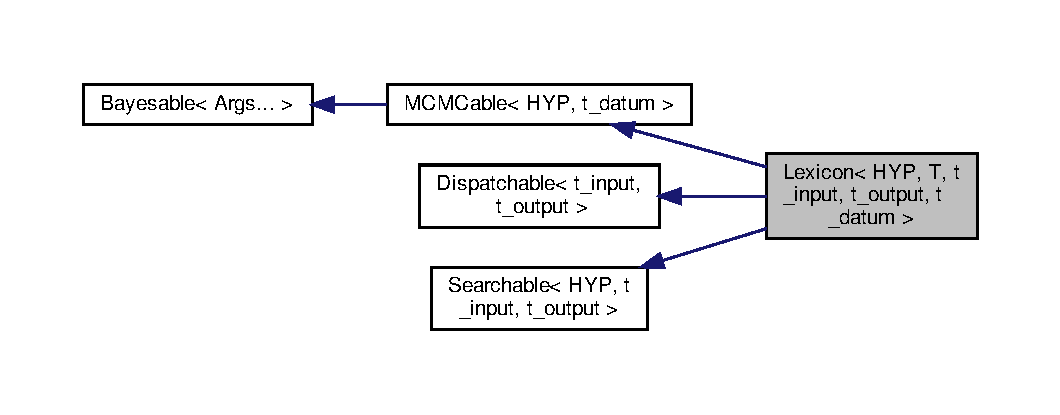
\includegraphics[width=350pt]{class_lexicon__inherit__graph}
\end{center}
\end{figure}


Collaboration diagram for Lexicon$<$ H\+YP, T, t\+\_\+input, t\+\_\+output, t\+\_\+datum $>$\+:\nopagebreak
\begin{figure}[H]
\begin{center}
\leavevmode
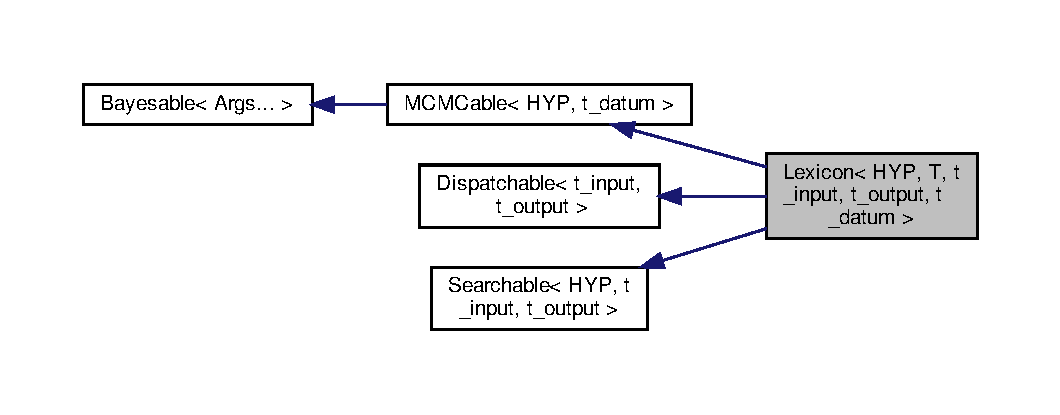
\includegraphics[width=350pt]{class_lexicon__coll__graph}
\end{center}
\end{figure}
\subsection*{Public Member Functions}
\begin{DoxyCompactItemize}
\item 
\hyperlink{class_lexicon_a8dde249de3f884484ff14de62a2c6df2}{Lexicon} (size\+\_\+t n)
\item 
\hyperlink{class_lexicon_a1b81e27f60f3e1cb7c0b376ac66aff45}{Lexicon} ()
\item 
virtual std\+::string \hyperlink{class_lexicon_a25895445cc5f7337e299e8d9dd14822c}{string} () const
\item 
virtual std\+::string \hyperlink{class_lexicon_a8eda74c4e7500b31a382c182ac60436a}{parseable} () const
\item 
virtual size\+\_\+t \hyperlink{class_lexicon_a4fed68bd543c0be81dfd63a2c8d219bd}{hash} () const
\begin{DoxyCompactList}\small\item\em Default hash function. \end{DoxyCompactList}\item 
virtual bool \hyperlink{class_lexicon_a852faeedb6cd12e629e601ebcad41729}{operator==} (const H\+YP \&l) const
\item 
bool \hyperlink{class_lexicon_a6d6b1b025ca707815a6776c3898503e4}{has\+\_\+valid\+\_\+indices} () const
\item 
bool \hyperlink{class_lexicon_aeb3e5f9f75e43f2147a22dee67fc8527}{check\+\_\+reachable} () const
\item 
virtual void \hyperlink{class_lexicon_af85ffc6944b66e92f760aaf7e3521d23}{push\+\_\+program} (Program \&s, short j)
\item 
virtual \hyperlink{_instruction_8h_a6202215407ab29590bb936ca2996cf64}{vmstatus\+\_\+t} \hyperlink{class_lexicon_a1c6b61ac505114f23441e3097163685b}{dispatch\+\_\+custom} (\hyperlink{class_instruction}{Instruction} i, \hyperlink{class_virtual_machine_pool}{Virtual\+Machine\+Pool}$<$ t\+\_\+input, t\+\_\+output $>$ $\ast$pool, \hyperlink{class_virtual_machine_state}{Virtual\+Machine\+State}$<$ t\+\_\+input, t\+\_\+output $>$ $\ast$vms, \hyperlink{class_dispatchable}{Dispatchable}$<$ t\+\_\+input, t\+\_\+output $>$ $\ast$loader)
\item 
virtual H\+YP \hyperlink{class_lexicon_a52a6e819264e04584320adca868aec4a}{copy\+\_\+and\+\_\+complete} () const
\item 
virtual double \hyperlink{class_lexicon_a1ac27e460a361cc90566b92365909324}{compute\+\_\+prior} ()
\begin{DoxyCompactList}\small\item\em Compute the prior -- defaultly not defined. \end{DoxyCompactList}\item 
virtual std\+::pair$<$ H\+YP, double $>$ \hyperlink{class_lexicon_a41a1955c8d373e85c3b926f161bf7e31}{propose} () const
\item 
virtual H\+YP \hyperlink{class_lexicon_a4ffff098d0f444d3e9ec543bbd228595}{restart} () const
\item 
int \hyperlink{class_lexicon_a1bad37e75741d1f9f9cf3fb11e9410d1}{neighbors} () const
\item 
H\+YP \hyperlink{class_lexicon_a2a5b2b625f4c7477c049c1fd8f0a2e3e}{make\+\_\+neighbor} (int k) const
\item 
bool \hyperlink{class_lexicon_ad48a8d79b77aed51caff4d10c7de43a1}{is\+\_\+evaluable} () const
\item 
virtual \hyperlink{class_discrete_distribution}{Discrete\+Distribution}$<$ t\+\_\+output $>$ \hyperlink{class_lexicon_aaaff682145f9cb15f7252420fe76f111}{call} (const t\+\_\+input x, const t\+\_\+output err)=0
\end{DoxyCompactItemize}
\subsection*{Static Public Member Functions}
\begin{DoxyCompactItemize}
\item 
static H\+YP \hyperlink{class_lexicon_a1a78d0be4350165b5757201b411f94f8}{from\+\_\+string} (\hyperlink{class_grammar}{Grammar} \&g, std\+::string s)
\end{DoxyCompactItemize}
\subsection*{Public Attributes}
\begin{DoxyCompactItemize}
\item 
std\+::vector$<$ T $>$ \hyperlink{class_lexicon_a030dd03b0f892b4bda7f8bc6ff3fc7df}{factors}
\end{DoxyCompactItemize}
\subsection*{Additional Inherited Members}


\subsection{Detailed Description}
\subsubsection*{template$<$typename H\+YP, typename T, typename t\+\_\+input, typename t\+\_\+output, typename t\+\_\+datum = default\+\_\+datum$<$t\+\_\+input, t\+\_\+output$>$$>$\newline
class Lexicon$<$ H\+Y\+P, T, t\+\_\+input, t\+\_\+output, t\+\_\+datum $>$}

\begin{DoxyAuthor}{Author}
piantado 
\end{DoxyAuthor}
\begin{DoxyDate}{Date}
29/01/20 
\end{DoxyDate}


\subsection{Constructor \& Destructor Documentation}
\mbox{\Hypertarget{class_lexicon_a8dde249de3f884484ff14de62a2c6df2}\label{class_lexicon_a8dde249de3f884484ff14de62a2c6df2}} 
\index{Lexicon@{Lexicon}!Lexicon@{Lexicon}}
\index{Lexicon@{Lexicon}!Lexicon@{Lexicon}}
\subsubsection{\texorpdfstring{Lexicon()}{Lexicon()}\hspace{0.1cm}{\footnotesize\ttfamily [1/2]}}
{\footnotesize\ttfamily template$<$typename H\+YP, typename T, typename t\+\_\+input, typename t\+\_\+output, typename t\+\_\+datum = default\+\_\+datum$<$t\+\_\+input, t\+\_\+output$>$$>$ \\
\hyperlink{class_lexicon}{Lexicon}$<$ H\+YP, T, t\+\_\+input, t\+\_\+output, \hyperlink{class_bayesable_a7c93a2eeab708378eb321745908718d4}{t\+\_\+datum} $>$\+::\hyperlink{class_lexicon}{Lexicon} (\begin{DoxyParamCaption}\item[{size\+\_\+t}]{n }\end{DoxyParamCaption})\hspace{0.3cm}{\ttfamily [inline]}}

\mbox{\Hypertarget{class_lexicon_a1b81e27f60f3e1cb7c0b376ac66aff45}\label{class_lexicon_a1b81e27f60f3e1cb7c0b376ac66aff45}} 
\index{Lexicon@{Lexicon}!Lexicon@{Lexicon}}
\index{Lexicon@{Lexicon}!Lexicon@{Lexicon}}
\subsubsection{\texorpdfstring{Lexicon()}{Lexicon()}\hspace{0.1cm}{\footnotesize\ttfamily [2/2]}}
{\footnotesize\ttfamily template$<$typename H\+YP, typename T, typename t\+\_\+input, typename t\+\_\+output, typename t\+\_\+datum = default\+\_\+datum$<$t\+\_\+input, t\+\_\+output$>$$>$ \\
\hyperlink{class_lexicon}{Lexicon}$<$ H\+YP, T, t\+\_\+input, t\+\_\+output, \hyperlink{class_bayesable_a7c93a2eeab708378eb321745908718d4}{t\+\_\+datum} $>$\+::\hyperlink{class_lexicon}{Lexicon} (\begin{DoxyParamCaption}{ }\end{DoxyParamCaption})\hspace{0.3cm}{\ttfamily [inline]}}



\subsection{Member Function Documentation}
\mbox{\Hypertarget{class_lexicon_aaaff682145f9cb15f7252420fe76f111}\label{class_lexicon_aaaff682145f9cb15f7252420fe76f111}} 
\index{Lexicon@{Lexicon}!call@{call}}
\index{call@{call}!Lexicon@{Lexicon}}
\subsubsection{\texorpdfstring{call()}{call()}}
{\footnotesize\ttfamily template$<$typename H\+YP, typename T, typename t\+\_\+input, typename t\+\_\+output, typename t\+\_\+datum = default\+\_\+datum$<$t\+\_\+input, t\+\_\+output$>$$>$ \\
virtual \hyperlink{class_discrete_distribution}{Discrete\+Distribution}$<$t\+\_\+output$>$ \hyperlink{class_lexicon}{Lexicon}$<$ H\+YP, T, t\+\_\+input, t\+\_\+output, \hyperlink{class_bayesable_a7c93a2eeab708378eb321745908718d4}{t\+\_\+datum} $>$\+::call (\begin{DoxyParamCaption}\item[{const t\+\_\+input}]{x,  }\item[{const t\+\_\+output}]{err }\end{DoxyParamCaption})\hspace{0.3cm}{\ttfamily [pure virtual]}}



Implemented in \hyperlink{class_my_hypothesis_a016146970c06041b3133f60152a80a24}{My\+Hypothesis}.

\mbox{\Hypertarget{class_lexicon_aeb3e5f9f75e43f2147a22dee67fc8527}\label{class_lexicon_aeb3e5f9f75e43f2147a22dee67fc8527}} 
\index{Lexicon@{Lexicon}!check\+\_\+reachable@{check\+\_\+reachable}}
\index{check\+\_\+reachable@{check\+\_\+reachable}!Lexicon@{Lexicon}}
\subsubsection{\texorpdfstring{check\+\_\+reachable()}{check\_reachable()}}
{\footnotesize\ttfamily template$<$typename H\+YP, typename T, typename t\+\_\+input, typename t\+\_\+output, typename t\+\_\+datum = default\+\_\+datum$<$t\+\_\+input, t\+\_\+output$>$$>$ \\
bool \hyperlink{class_lexicon}{Lexicon}$<$ H\+YP, T, t\+\_\+input, t\+\_\+output, \hyperlink{class_bayesable_a7c93a2eeab708378eb321745908718d4}{t\+\_\+datum} $>$\+::check\+\_\+reachable (\begin{DoxyParamCaption}{ }\end{DoxyParamCaption}) const\hspace{0.3cm}{\ttfamily [inline]}}

Check if the last factor call everything else transitively (e.\+g. are we \char`\"{}wasting\char`\"{} factors) We do this by making a graph of what factors call which others and then computing the transitive closure. \begin{DoxyReturn}{Returns}

\end{DoxyReturn}
\mbox{\Hypertarget{class_lexicon_a1ac27e460a361cc90566b92365909324}\label{class_lexicon_a1ac27e460a361cc90566b92365909324}} 
\index{Lexicon@{Lexicon}!compute\+\_\+prior@{compute\+\_\+prior}}
\index{compute\+\_\+prior@{compute\+\_\+prior}!Lexicon@{Lexicon}}
\subsubsection{\texorpdfstring{compute\+\_\+prior()}{compute\_prior()}}
{\footnotesize\ttfamily template$<$typename H\+YP, typename T, typename t\+\_\+input, typename t\+\_\+output, typename t\+\_\+datum = default\+\_\+datum$<$t\+\_\+input, t\+\_\+output$>$$>$ \\
virtual double \hyperlink{class_lexicon}{Lexicon}$<$ H\+YP, T, t\+\_\+input, t\+\_\+output, \hyperlink{class_bayesable_a7c93a2eeab708378eb321745908718d4}{t\+\_\+datum} $>$\+::compute\+\_\+prior (\begin{DoxyParamCaption}{ }\end{DoxyParamCaption})\hspace{0.3cm}{\ttfamily [inline]}, {\ttfamily [virtual]}}



Compute the prior -- defaultly not defined. 



Implements \hyperlink{class_bayesable_a9aa752f0adff1b95f8957b91fc928649}{Bayesable$<$ Args... $>$}.



Reimplemented in \hyperlink{class_my_hypothesis_a67752bb4ba61994ef0cb64f7f9031f7f}{My\+Hypothesis}.

\mbox{\Hypertarget{class_lexicon_a52a6e819264e04584320adca868aec4a}\label{class_lexicon_a52a6e819264e04584320adca868aec4a}} 
\index{Lexicon@{Lexicon}!copy\+\_\+and\+\_\+complete@{copy\+\_\+and\+\_\+complete}}
\index{copy\+\_\+and\+\_\+complete@{copy\+\_\+and\+\_\+complete}!Lexicon@{Lexicon}}
\subsubsection{\texorpdfstring{copy\+\_\+and\+\_\+complete()}{copy\_and\_complete()}}
{\footnotesize\ttfamily template$<$typename H\+YP, typename T, typename t\+\_\+input, typename t\+\_\+output, typename t\+\_\+datum = default\+\_\+datum$<$t\+\_\+input, t\+\_\+output$>$$>$ \\
virtual H\+YP \hyperlink{class_lexicon}{Lexicon}$<$ H\+YP, T, t\+\_\+input, t\+\_\+output, \hyperlink{class_bayesable_a7c93a2eeab708378eb321745908718d4}{t\+\_\+datum} $>$\+::copy\+\_\+and\+\_\+complete (\begin{DoxyParamCaption}{ }\end{DoxyParamCaption}) const\hspace{0.3cm}{\ttfamily [inline]}, {\ttfamily [virtual]}}

\mbox{\Hypertarget{class_lexicon_a1c6b61ac505114f23441e3097163685b}\label{class_lexicon_a1c6b61ac505114f23441e3097163685b}} 
\index{Lexicon@{Lexicon}!dispatch\+\_\+custom@{dispatch\+\_\+custom}}
\index{dispatch\+\_\+custom@{dispatch\+\_\+custom}!Lexicon@{Lexicon}}
\subsubsection{\texorpdfstring{dispatch\+\_\+custom()}{dispatch\_custom()}}
{\footnotesize\ttfamily template$<$typename H\+YP, typename T, typename t\+\_\+input, typename t\+\_\+output, typename t\+\_\+datum = default\+\_\+datum$<$t\+\_\+input, t\+\_\+output$>$$>$ \\
virtual \hyperlink{_instruction_8h_a6202215407ab29590bb936ca2996cf64}{vmstatus\+\_\+t} \hyperlink{class_lexicon}{Lexicon}$<$ H\+YP, T, t\+\_\+input, t\+\_\+output, \hyperlink{class_bayesable_a7c93a2eeab708378eb321745908718d4}{t\+\_\+datum} $>$\+::dispatch\+\_\+custom (\begin{DoxyParamCaption}\item[{\hyperlink{class_instruction}{Instruction}}]{i,  }\item[{\hyperlink{class_virtual_machine_pool}{Virtual\+Machine\+Pool}$<$ t\+\_\+input, t\+\_\+output $>$ $\ast$}]{pool,  }\item[{\hyperlink{class_virtual_machine_state}{Virtual\+Machine\+State}$<$ t\+\_\+input, t\+\_\+output $>$ $\ast$}]{vms,  }\item[{\hyperlink{class_dispatchable}{Dispatchable}$<$ t\+\_\+input, t\+\_\+output $>$ $\ast$}]{loader }\end{DoxyParamCaption})\hspace{0.3cm}{\ttfamily [inline]}, {\ttfamily [virtual]}}



Implements \hyperlink{class_dispatchable_a6d2bd844b0e55378d29ed85e718d0a77}{Dispatchable$<$ t\+\_\+input, t\+\_\+output $>$}.

\mbox{\Hypertarget{class_lexicon_a1a78d0be4350165b5757201b411f94f8}\label{class_lexicon_a1a78d0be4350165b5757201b411f94f8}} 
\index{Lexicon@{Lexicon}!from\+\_\+string@{from\+\_\+string}}
\index{from\+\_\+string@{from\+\_\+string}!Lexicon@{Lexicon}}
\subsubsection{\texorpdfstring{from\+\_\+string()}{from\_string()}}
{\footnotesize\ttfamily template$<$typename H\+YP, typename T, typename t\+\_\+input, typename t\+\_\+output, typename t\+\_\+datum = default\+\_\+datum$<$t\+\_\+input, t\+\_\+output$>$$>$ \\
static H\+YP \hyperlink{class_lexicon}{Lexicon}$<$ H\+YP, T, t\+\_\+input, t\+\_\+output, \hyperlink{class_bayesable_a7c93a2eeab708378eb321745908718d4}{t\+\_\+datum} $>$\+::from\+\_\+string (\begin{DoxyParamCaption}\item[{\hyperlink{class_grammar}{Grammar} \&}]{g,  }\item[{std\+::string}]{s }\end{DoxyParamCaption})\hspace{0.3cm}{\ttfamily [inline]}, {\ttfamily [static]}}

Convert a string to a lexicon of this type 
\begin{DoxyParams}{Parameters}
{\em g} & \\
\hline
{\em s} & \\
\hline
\end{DoxyParams}
\begin{DoxyReturn}{Returns}

\end{DoxyReturn}
\mbox{\Hypertarget{class_lexicon_a6d6b1b025ca707815a6776c3898503e4}\label{class_lexicon_a6d6b1b025ca707815a6776c3898503e4}} 
\index{Lexicon@{Lexicon}!has\+\_\+valid\+\_\+indices@{has\+\_\+valid\+\_\+indices}}
\index{has\+\_\+valid\+\_\+indices@{has\+\_\+valid\+\_\+indices}!Lexicon@{Lexicon}}
\subsubsection{\texorpdfstring{has\+\_\+valid\+\_\+indices()}{has\_valid\_indices()}}
{\footnotesize\ttfamily template$<$typename H\+YP, typename T, typename t\+\_\+input, typename t\+\_\+output, typename t\+\_\+datum = default\+\_\+datum$<$t\+\_\+input, t\+\_\+output$>$$>$ \\
bool \hyperlink{class_lexicon}{Lexicon}$<$ H\+YP, T, t\+\_\+input, t\+\_\+output, \hyperlink{class_bayesable_a7c93a2eeab708378eb321745908718d4}{t\+\_\+datum} $>$\+::has\+\_\+valid\+\_\+indices (\begin{DoxyParamCaption}{ }\end{DoxyParamCaption}) const\hspace{0.3cm}{\ttfamily [inline]}}

A lexicon has valid indices if calls to op\+\_\+\+R\+E\+C\+U\+R\+SE, op\+\_\+\+M\+E\+M\+\_\+\+R\+E\+C\+U\+R\+SE, op\+\_\+\+S\+A\+F\+E\+\_\+\+R\+E\+C\+U\+R\+SE, and op\+\_\+\+S\+A\+F\+E\+\_\+\+M\+E\+M\+\_\+\+R\+E\+C\+U\+R\+SE all have arguments that are less than the size. (So this places no restrictions on the calling earlier factors) \begin{DoxyReturn}{Returns}

\end{DoxyReturn}
\mbox{\Hypertarget{class_lexicon_a4fed68bd543c0be81dfd63a2c8d219bd}\label{class_lexicon_a4fed68bd543c0be81dfd63a2c8d219bd}} 
\index{Lexicon@{Lexicon}!hash@{hash}}
\index{hash@{hash}!Lexicon@{Lexicon}}
\subsubsection{\texorpdfstring{hash()}{hash()}}
{\footnotesize\ttfamily template$<$typename H\+YP, typename T, typename t\+\_\+input, typename t\+\_\+output, typename t\+\_\+datum = default\+\_\+datum$<$t\+\_\+input, t\+\_\+output$>$$>$ \\
virtual size\+\_\+t \hyperlink{class_lexicon}{Lexicon}$<$ H\+YP, T, t\+\_\+input, t\+\_\+output, \hyperlink{class_bayesable_a7c93a2eeab708378eb321745908718d4}{t\+\_\+datum} $>$\+::hash (\begin{DoxyParamCaption}{ }\end{DoxyParamCaption}) const\hspace{0.3cm}{\ttfamily [inline]}, {\ttfamily [virtual]}}



Default hash function. 

Hash a \hyperlink{class_lexicon}{Lexicon} by hashing each part \begin{DoxyReturn}{Returns}

\end{DoxyReturn}


Implements \hyperlink{class_bayesable_ab77a023d33951448e6edb2e1bc79c5ae}{Bayesable$<$ Args... $>$}.

\mbox{\Hypertarget{class_lexicon_ad48a8d79b77aed51caff4d10c7de43a1}\label{class_lexicon_ad48a8d79b77aed51caff4d10c7de43a1}} 
\index{Lexicon@{Lexicon}!is\+\_\+evaluable@{is\+\_\+evaluable}}
\index{is\+\_\+evaluable@{is\+\_\+evaluable}!Lexicon@{Lexicon}}
\subsubsection{\texorpdfstring{is\+\_\+evaluable()}{is\_evaluable()}}
{\footnotesize\ttfamily template$<$typename H\+YP, typename T, typename t\+\_\+input, typename t\+\_\+output, typename t\+\_\+datum = default\+\_\+datum$<$t\+\_\+input, t\+\_\+output$>$$>$ \\
bool \hyperlink{class_lexicon}{Lexicon}$<$ H\+YP, T, t\+\_\+input, t\+\_\+output, \hyperlink{class_bayesable_a7c93a2eeab708378eb321745908718d4}{t\+\_\+datum} $>$\+::is\+\_\+evaluable (\begin{DoxyParamCaption}{ }\end{DoxyParamCaption}) const\hspace{0.3cm}{\ttfamily [inline]}, {\ttfamily [virtual]}}



Implements \hyperlink{class_searchable_aae16f1cb01f140f4033f6f67dc9753b6}{Searchable$<$ H\+Y\+P, t\+\_\+input, t\+\_\+output $>$}.

\mbox{\Hypertarget{class_lexicon_a2a5b2b625f4c7477c049c1fd8f0a2e3e}\label{class_lexicon_a2a5b2b625f4c7477c049c1fd8f0a2e3e}} 
\index{Lexicon@{Lexicon}!make\+\_\+neighbor@{make\+\_\+neighbor}}
\index{make\+\_\+neighbor@{make\+\_\+neighbor}!Lexicon@{Lexicon}}
\subsubsection{\texorpdfstring{make\+\_\+neighbor()}{make\_neighbor()}}
{\footnotesize\ttfamily template$<$typename H\+YP, typename T, typename t\+\_\+input, typename t\+\_\+output, typename t\+\_\+datum = default\+\_\+datum$<$t\+\_\+input, t\+\_\+output$>$$>$ \\
H\+YP \hyperlink{class_lexicon}{Lexicon}$<$ H\+YP, T, t\+\_\+input, t\+\_\+output, \hyperlink{class_bayesable_a7c93a2eeab708378eb321745908718d4}{t\+\_\+datum} $>$\+::make\+\_\+neighbor (\begin{DoxyParamCaption}\item[{int}]{k }\end{DoxyParamCaption}) const\hspace{0.3cm}{\ttfamily [inline]}, {\ttfamily [virtual]}}



Implements \hyperlink{class_searchable_a64bda92cc9314dae7aff31f4444a93e6}{Searchable$<$ H\+Y\+P, t\+\_\+input, t\+\_\+output $>$}.

\mbox{\Hypertarget{class_lexicon_a1bad37e75741d1f9f9cf3fb11e9410d1}\label{class_lexicon_a1bad37e75741d1f9f9cf3fb11e9410d1}} 
\index{Lexicon@{Lexicon}!neighbors@{neighbors}}
\index{neighbors@{neighbors}!Lexicon@{Lexicon}}
\subsubsection{\texorpdfstring{neighbors()}{neighbors()}}
{\footnotesize\ttfamily template$<$typename H\+YP, typename T, typename t\+\_\+input, typename t\+\_\+output, typename t\+\_\+datum = default\+\_\+datum$<$t\+\_\+input, t\+\_\+output$>$$>$ \\
int \hyperlink{class_lexicon}{Lexicon}$<$ H\+YP, T, t\+\_\+input, t\+\_\+output, \hyperlink{class_bayesable_a7c93a2eeab708378eb321745908718d4}{t\+\_\+datum} $>$\+::neighbors (\begin{DoxyParamCaption}{ }\end{DoxyParamCaption}) const\hspace{0.3cm}{\ttfamily [inline]}, {\ttfamily [virtual]}}



Implements \hyperlink{class_searchable_a0450c35a21c5940a63560aa24b4ff0cc}{Searchable$<$ H\+Y\+P, t\+\_\+input, t\+\_\+output $>$}.

\mbox{\Hypertarget{class_lexicon_a852faeedb6cd12e629e601ebcad41729}\label{class_lexicon_a852faeedb6cd12e629e601ebcad41729}} 
\index{Lexicon@{Lexicon}!operator==@{operator==}}
\index{operator==@{operator==}!Lexicon@{Lexicon}}
\subsubsection{\texorpdfstring{operator==()}{operator==()}}
{\footnotesize\ttfamily template$<$typename H\+YP, typename T, typename t\+\_\+input, typename t\+\_\+output, typename t\+\_\+datum = default\+\_\+datum$<$t\+\_\+input, t\+\_\+output$>$$>$ \\
virtual bool \hyperlink{class_lexicon}{Lexicon}$<$ H\+YP, T, t\+\_\+input, t\+\_\+output, \hyperlink{class_bayesable_a7c93a2eeab708378eb321745908718d4}{t\+\_\+datum} $>$\+::operator== (\begin{DoxyParamCaption}\item[{const H\+YP \&}]{l }\end{DoxyParamCaption}) const\hspace{0.3cm}{\ttfamily [inline]}, {\ttfamily [virtual]}}

Equality checks equality on each part 
\begin{DoxyParams}{Parameters}
{\em l} & \\
\hline
\end{DoxyParams}
\begin{DoxyReturn}{Returns}

\end{DoxyReturn}


Implements \hyperlink{class_m_c_m_cable_aa73001ec3bb0cf0c618281dfa998f2f1}{M\+C\+M\+Cable$<$ H\+Y\+P, t\+\_\+datum $>$}.

\mbox{\Hypertarget{class_lexicon_a8eda74c4e7500b31a382c182ac60436a}\label{class_lexicon_a8eda74c4e7500b31a382c182ac60436a}} 
\index{Lexicon@{Lexicon}!parseable@{parseable}}
\index{parseable@{parseable}!Lexicon@{Lexicon}}
\subsubsection{\texorpdfstring{parseable()}{parseable()}}
{\footnotesize\ttfamily template$<$typename H\+YP, typename T, typename t\+\_\+input, typename t\+\_\+output, typename t\+\_\+datum = default\+\_\+datum$<$t\+\_\+input, t\+\_\+output$>$$>$ \\
virtual std\+::string \hyperlink{class_lexicon}{Lexicon}$<$ H\+YP, T, t\+\_\+input, t\+\_\+output, \hyperlink{class_bayesable_a7c93a2eeab708378eb321745908718d4}{t\+\_\+datum} $>$\+::parseable (\begin{DoxyParamCaption}{ }\end{DoxyParamCaption}) const\hspace{0.3cm}{\ttfamily [inline]}, {\ttfamily [virtual]}}

Convert to a parseable format (using a delimiter for each factor) \begin{DoxyReturn}{Returns}

\end{DoxyReturn}
\mbox{\Hypertarget{class_lexicon_a41a1955c8d373e85c3b926f161bf7e31}\label{class_lexicon_a41a1955c8d373e85c3b926f161bf7e31}} 
\index{Lexicon@{Lexicon}!propose@{propose}}
\index{propose@{propose}!Lexicon@{Lexicon}}
\subsubsection{\texorpdfstring{propose()}{propose()}}
{\footnotesize\ttfamily template$<$typename H\+YP, typename T, typename t\+\_\+input, typename t\+\_\+output, typename t\+\_\+datum = default\+\_\+datum$<$t\+\_\+input, t\+\_\+output$>$$>$ \\
virtual std\+::pair$<$H\+YP,double$>$ \hyperlink{class_lexicon}{Lexicon}$<$ H\+YP, T, t\+\_\+input, t\+\_\+output, \hyperlink{class_bayesable_a7c93a2eeab708378eb321745908718d4}{t\+\_\+datum} $>$\+::propose (\begin{DoxyParamCaption}{ }\end{DoxyParamCaption}) const\hspace{0.3cm}{\ttfamily [inline]}, {\ttfamily [virtual]}}

This proposal guarantees that there will be at least one factor that is proposed to. To do this, we draw random numbers on 2$\ast$$\ast$factors.size()-\/1 and then use the bits of that integer to determine which factors to propose to. \begin{DoxyReturn}{Returns}

\end{DoxyReturn}


Implements \hyperlink{class_m_c_m_cable_ab119a14256ab92c5c1e941f8492df830}{M\+C\+M\+Cable$<$ H\+Y\+P, t\+\_\+datum $>$}.

\mbox{\Hypertarget{class_lexicon_af85ffc6944b66e92f760aaf7e3521d23}\label{class_lexicon_af85ffc6944b66e92f760aaf7e3521d23}} 
\index{Lexicon@{Lexicon}!push\+\_\+program@{push\+\_\+program}}
\index{push\+\_\+program@{push\+\_\+program}!Lexicon@{Lexicon}}
\subsubsection{\texorpdfstring{push\+\_\+program()}{push\_program()}}
{\footnotesize\ttfamily template$<$typename H\+YP, typename T, typename t\+\_\+input, typename t\+\_\+output, typename t\+\_\+datum = default\+\_\+datum$<$t\+\_\+input, t\+\_\+output$>$$>$ \\
virtual void \hyperlink{class_lexicon}{Lexicon}$<$ H\+YP, T, t\+\_\+input, t\+\_\+output, \hyperlink{class_bayesable_a7c93a2eeab708378eb321745908718d4}{t\+\_\+datum} $>$\+::push\+\_\+program (\begin{DoxyParamCaption}\item[{Program \&}]{s,  }\item[{short}]{j }\end{DoxyParamCaption})\hspace{0.3cm}{\ttfamily [inline]}, {\ttfamily [virtual]}}

Put factor j onto program s 
\begin{DoxyParams}{Parameters}
{\em s} & \\
\hline
{\em j} & \\
\hline
\end{DoxyParams}


Implements \hyperlink{class_dispatchable_a9339c2906f7c8dadbe1d0ca79dd9bb11}{Dispatchable$<$ t\+\_\+input, t\+\_\+output $>$}.

\mbox{\Hypertarget{class_lexicon_a4ffff098d0f444d3e9ec543bbd228595}\label{class_lexicon_a4ffff098d0f444d3e9ec543bbd228595}} 
\index{Lexicon@{Lexicon}!restart@{restart}}
\index{restart@{restart}!Lexicon@{Lexicon}}
\subsubsection{\texorpdfstring{restart()}{restart()}}
{\footnotesize\ttfamily template$<$typename H\+YP, typename T, typename t\+\_\+input, typename t\+\_\+output, typename t\+\_\+datum = default\+\_\+datum$<$t\+\_\+input, t\+\_\+output$>$$>$ \\
virtual H\+YP \hyperlink{class_lexicon}{Lexicon}$<$ H\+YP, T, t\+\_\+input, t\+\_\+output, \hyperlink{class_bayesable_a7c93a2eeab708378eb321745908718d4}{t\+\_\+datum} $>$\+::restart (\begin{DoxyParamCaption}{ }\end{DoxyParamCaption}) const\hspace{0.3cm}{\ttfamily [inline]}, {\ttfamily [virtual]}}



Implements \hyperlink{class_m_c_m_cable_a220d6c4ca73e20441c14fa5bd3e090d3}{M\+C\+M\+Cable$<$ H\+Y\+P, t\+\_\+datum $>$}.

\mbox{\Hypertarget{class_lexicon_a25895445cc5f7337e299e8d9dd14822c}\label{class_lexicon_a25895445cc5f7337e299e8d9dd14822c}} 
\index{Lexicon@{Lexicon}!string@{string}}
\index{string@{string}!Lexicon@{Lexicon}}
\subsubsection{\texorpdfstring{string()}{string()}}
{\footnotesize\ttfamily template$<$typename H\+YP, typename T, typename t\+\_\+input, typename t\+\_\+output, typename t\+\_\+datum = default\+\_\+datum$<$t\+\_\+input, t\+\_\+output$>$$>$ \\
virtual std\+::string \hyperlink{class_lexicon}{Lexicon}$<$ H\+YP, T, t\+\_\+input, t\+\_\+output, \hyperlink{class_bayesable_a7c93a2eeab708378eb321745908718d4}{t\+\_\+datum} $>$\+::string (\begin{DoxyParamCaption}{ }\end{DoxyParamCaption}) const\hspace{0.3cm}{\ttfamily [inline]}, {\ttfamily [virtual]}}

A\+Convert a lexicon to a string -- defaultly includes all arguments. \begin{DoxyReturn}{Returns}

\end{DoxyReturn}


Implements \hyperlink{class_bayesable_a2ec58e98bf37a90ac3d45a7713c6d5ea}{Bayesable$<$ Args... $>$}.



\subsection{Member Data Documentation}
\mbox{\Hypertarget{class_lexicon_a030dd03b0f892b4bda7f8bc6ff3fc7df}\label{class_lexicon_a030dd03b0f892b4bda7f8bc6ff3fc7df}} 
\index{Lexicon@{Lexicon}!factors@{factors}}
\index{factors@{factors}!Lexicon@{Lexicon}}
\subsubsection{\texorpdfstring{factors}{factors}}
{\footnotesize\ttfamily template$<$typename H\+YP, typename T, typename t\+\_\+input, typename t\+\_\+output, typename t\+\_\+datum = default\+\_\+datum$<$t\+\_\+input, t\+\_\+output$>$$>$ \\
std\+::vector$<$T$>$ \hyperlink{class_lexicon}{Lexicon}$<$ H\+YP, T, t\+\_\+input, t\+\_\+output, \hyperlink{class_bayesable_a7c93a2eeab708378eb321745908718d4}{t\+\_\+datum} $>$\+::factors}



The documentation for this class was generated from the following file\+:\begin{DoxyCompactItemize}
\item 
src/\+Hypotheses/\hyperlink{_lexicon_8h}{Lexicon.\+h}\end{DoxyCompactItemize}

\hypertarget{class_l_o_t_hypothesis}{}\section{L\+O\+T\+Hypothesis$<$ H\+YP, T, t\+\_\+input, t\+\_\+output, \+\_\+t\+\_\+datum, \+\_\+t\+\_\+data $>$ Class Template Reference}
\label{class_l_o_t_hypothesis}\index{L\+O\+T\+Hypothesis$<$ H\+Y\+P, T, t\+\_\+input, t\+\_\+output, \+\_\+t\+\_\+datum, \+\_\+t\+\_\+data $>$@{L\+O\+T\+Hypothesis$<$ H\+Y\+P, T, t\+\_\+input, t\+\_\+output, \+\_\+t\+\_\+datum, \+\_\+t\+\_\+data $>$}}


{\ttfamily \#include $<$L\+O\+T\+Hypothesis.\+h$>$}



Inheritance diagram for L\+O\+T\+Hypothesis$<$ H\+YP, T, t\+\_\+input, t\+\_\+output, \+\_\+t\+\_\+datum, \+\_\+t\+\_\+data $>$\+:\nopagebreak
\begin{figure}[H]
\begin{center}
\leavevmode
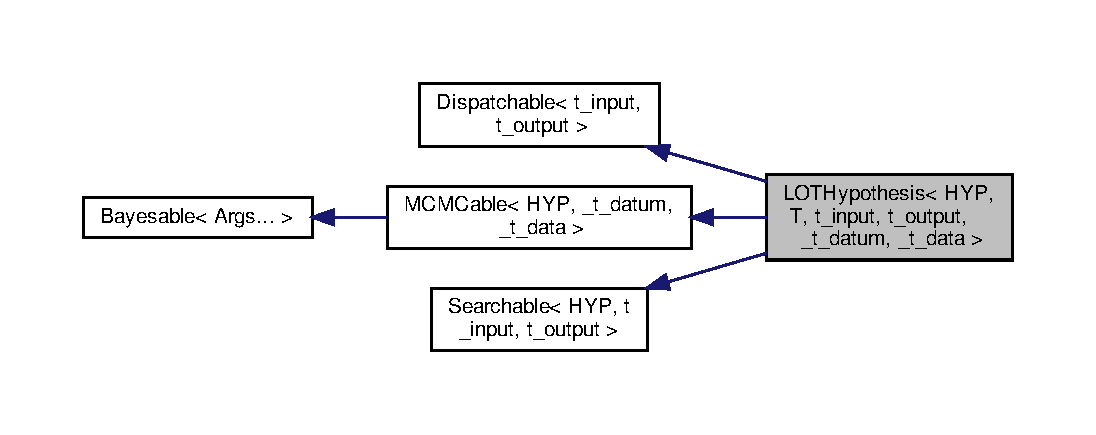
\includegraphics[width=350pt]{class_l_o_t_hypothesis__inherit__graph}
\end{center}
\end{figure}


Collaboration diagram for L\+O\+T\+Hypothesis$<$ H\+YP, T, t\+\_\+input, t\+\_\+output, \+\_\+t\+\_\+datum, \+\_\+t\+\_\+data $>$\+:\nopagebreak
\begin{figure}[H]
\begin{center}
\leavevmode
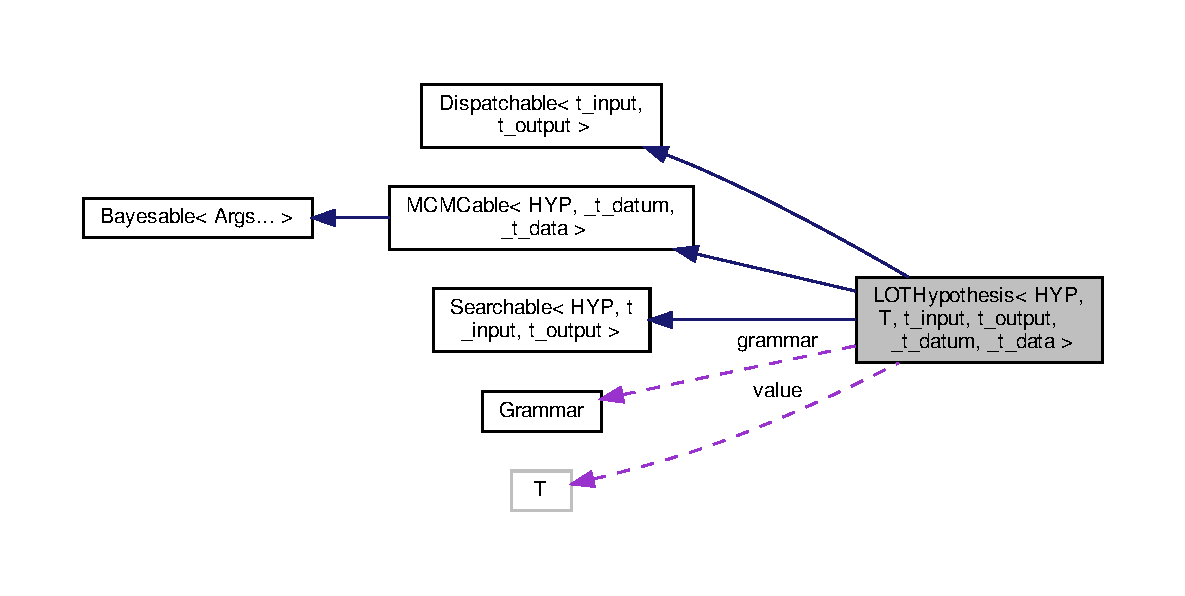
\includegraphics[width=350pt]{class_l_o_t_hypothesis__coll__graph}
\end{center}
\end{figure}
\subsection*{Public Types}
\begin{DoxyCompactItemize}
\item 
typedef \hyperlink{class_bayesable}{Bayesable}$<$ \+\_\+t\+\_\+datum, \+\_\+t\+\_\+data $>$\+::\hyperlink{class_l_o_t_hypothesis_a3a7b2c5fb3e2b5d70fa80b485b0b98f5}{t\+\_\+data} \hyperlink{class_l_o_t_hypothesis_a3a7b2c5fb3e2b5d70fa80b485b0b98f5}{t\+\_\+data}
\item 
typedef \hyperlink{class_bayesable}{Bayesable}$<$ \+\_\+t\+\_\+datum, \+\_\+t\+\_\+data $>$\+::\hyperlink{class_l_o_t_hypothesis_a26d0ecfa6a367f32276d36cd01c0cead}{t\+\_\+datum} \hyperlink{class_l_o_t_hypothesis_a26d0ecfa6a367f32276d36cd01c0cead}{t\+\_\+datum}
\end{DoxyCompactItemize}
\subsection*{Public Member Functions}
\begin{DoxyCompactItemize}
\item 
\hyperlink{class_l_o_t_hypothesis_a47dcb988a9cb4bba00263851d697fc12}{L\+O\+T\+Hypothesis} (\hyperlink{class_grammar}{Grammar} $\ast$g=nullptr)
\item 
\hyperlink{class_l_o_t_hypothesis_abfb19603c9bdda8b8b8c682b6cdc6e03}{L\+O\+T\+Hypothesis} (\hyperlink{class_grammar}{Grammar} $\ast$g, T \&\&x)
\item 
\hyperlink{class_l_o_t_hypothesis_a3123d5e4e140ca24fdaa568bd2b17644}{L\+O\+T\+Hypothesis} (\hyperlink{class_grammar}{Grammar} $\ast$g, T \&x)
\item 
\hyperlink{class_l_o_t_hypothesis_a09216df69fea175ccb5ffc1a947b8287}{L\+O\+T\+Hypothesis} (\hyperlink{class_grammar}{Grammar} $\ast$g, std\+::string s)
\item 
virtual std\+::pair$<$ H\+YP, double $>$ \hyperlink{class_l_o_t_hypothesis_a5ae913b145b15308d5817c6e7b1da14d}{propose} () const override
\item 
virtual H\+YP \hyperlink{class_l_o_t_hypothesis_aec55db1efe43a1ce4bb4a2daacd0f1b7}{restart} () const override
\item 
void \hyperlink{class_l_o_t_hypothesis_a873355cca03609ac0ab405d29314e591}{set\+\_\+value} (T \&v)
\item 
void \hyperlink{class_l_o_t_hypothesis_ac07e0957d2e586f2cc84821795d5c462}{set\+\_\+value} (T \&\&v)
\item 
virtual double \hyperlink{class_l_o_t_hypothesis_a80eea871bc115e4ef585f75f06857b39}{compute\+\_\+prior} () override
\begin{DoxyCompactList}\small\item\em Compute the prior -- defaultly not defined. \end{DoxyCompactList}\item 
virtual double \hyperlink{class_l_o_t_hypothesis_a835f1aafdd4bc4748c343edb80517956}{compute\+\_\+single\+\_\+likelihood} (const \hyperlink{class_l_o_t_hypothesis_a26d0ecfa6a367f32276d36cd01c0cead}{t\+\_\+datum} \&datum) override
\item 
virtual void \hyperlink{class_l_o_t_hypothesis_aff3a378ab1137e2b46f225a028343a1c}{push\+\_\+program} (Program \&s, short k=0) override
\item 
virtual \hyperlink{class_discrete_distribution}{Discrete\+Distribution}$<$ t\+\_\+output $>$ \hyperlink{class_l_o_t_hypothesis_a592d67c976a67982251239b415e0a861}{call} (const t\+\_\+input x, const t\+\_\+output err, \hyperlink{class_dispatchable}{Dispatchable}$<$ t\+\_\+input, t\+\_\+output $>$ $\ast$loader, unsigned long max\+\_\+steps=2048, unsigned long max\+\_\+outputs=256, double minlp=-\/10.\+0)
\item 
virtual \hyperlink{class_discrete_distribution}{Discrete\+Distribution}$<$ t\+\_\+output $>$ \hyperlink{class_l_o_t_hypothesis_a48858f5add54c1886d946e641b08062a}{call} (const t\+\_\+input x, const t\+\_\+output err)
\item 
auto \hyperlink{class_l_o_t_hypothesis_ae64a27eeb271316fd76cf26a86fff7e6}{operator()} (const t\+\_\+input x, const t\+\_\+output err)
\item 
virtual t\+\_\+output \hyperlink{class_l_o_t_hypothesis_ad792b258bdb4b0828f11ac721f52e704}{call\+One} (const t\+\_\+input x, const t\+\_\+output err, \hyperlink{class_dispatchable}{Dispatchable}$<$ t\+\_\+input, t\+\_\+output $>$ $\ast$loader=nullptr)
\item 
virtual std\+::string \hyperlink{class_l_o_t_hypothesis_a5c91fd3b7ef4ebc585413d723cd17e7e}{string} () const override
\item 
virtual std\+::string \hyperlink{class_l_o_t_hypothesis_a1584633d01abe30a6f69d0664c1e137a}{parseable} () const
\item 
virtual size\+\_\+t \hyperlink{class_l_o_t_hypothesis_aa6859da0a3b422c32b1be2ffa025631a}{hash} () const override
\begin{DoxyCompactList}\small\item\em Default hash function. \end{DoxyCompactList}\item 
virtual bool \hyperlink{class_l_o_t_hypothesis_a198d0632ce824b9547810084abadfb2e}{operator==} (const H\+YP \&h) const override
\item 
virtual \hyperlink{_instruction_8h_a6202215407ab29590bb936ca2996cf64}{vmstatus\+\_\+t} \hyperlink{class_l_o_t_hypothesis_a9aade3ee6939a58e5d5b53505cfb2e7a}{dispatch\+\_\+custom} (\hyperlink{class_instruction}{Instruction} i, \hyperlink{class_virtual_machine_pool}{Virtual\+Machine\+Pool}$<$ t\+\_\+input, t\+\_\+output $>$ $\ast$pool, \hyperlink{class_virtual_machine_state}{Virtual\+Machine\+State}$<$ t\+\_\+input, t\+\_\+output $>$ $\ast$vms, \hyperlink{class_dispatchable}{Dispatchable}$<$ t\+\_\+input, t\+\_\+output $>$ $\ast$loader) override
\item 
virtual H\+YP \hyperlink{class_l_o_t_hypothesis_af0274e15c0e19e8f42324b7099e2b4a1}{copy\+\_\+and\+\_\+complete} () const
\item 
virtual int \hyperlink{class_l_o_t_hypothesis_ac74e874f6b677dc1c013602907627be7}{neighbors} () const override
\item 
virtual H\+YP \hyperlink{class_l_o_t_hypothesis_ae7771176b8b2599f42c75318ee0e9164}{make\+\_\+neighbor} (int k) const override
\item 
virtual bool \hyperlink{class_l_o_t_hypothesis_a68dedaeae92b25b0450f2dc1bd95a35b}{is\+\_\+evaluable} () const override
\end{DoxyCompactItemize}
\subsection*{Static Public Member Functions}
\begin{DoxyCompactItemize}
\item 
static H\+YP \hyperlink{class_l_o_t_hypothesis_a684d3208f52e10c61418dc0707142a30}{from\+\_\+string} (\hyperlink{class_grammar}{Grammar} \&g, std\+::string s)
\end{DoxyCompactItemize}
\subsection*{Public Attributes}
\begin{DoxyCompactItemize}
\item 
\hyperlink{class_grammar}{Grammar} $\ast$ \hyperlink{class_l_o_t_hypothesis_aa7cf638b5d680794e33aa5eb4bd36b09}{grammar}
\item 
T \hyperlink{class_l_o_t_hypothesis_aff7455a900ffb91790e5235119676a80}{value}
\end{DoxyCompactItemize}
\subsection*{Static Public Attributes}
\begin{DoxyCompactItemize}
\item 
static const size\+\_\+t \hyperlink{class_l_o_t_hypothesis_ab262eb592887136a986f5b2649397eca}{M\+A\+X\+\_\+\+N\+O\+D\+ES} = 64
\end{DoxyCompactItemize}


\subsection{Member Typedef Documentation}
\mbox{\Hypertarget{class_l_o_t_hypothesis_a3a7b2c5fb3e2b5d70fa80b485b0b98f5}\label{class_l_o_t_hypothesis_a3a7b2c5fb3e2b5d70fa80b485b0b98f5}} 
\index{L\+O\+T\+Hypothesis@{L\+O\+T\+Hypothesis}!t\+\_\+data@{t\+\_\+data}}
\index{t\+\_\+data@{t\+\_\+data}!L\+O\+T\+Hypothesis@{L\+O\+T\+Hypothesis}}
\subsubsection{\texorpdfstring{t\+\_\+data}{t\_data}}
{\footnotesize\ttfamily template$<$typename H\+YP, typename T, typename t\+\_\+input, typename t\+\_\+output, typename \+\_\+t\+\_\+datum = default\+\_\+datum$<$t\+\_\+input, t\+\_\+output$>$, typename \+\_\+t\+\_\+data = std\+::vector$<$\+\_\+t\+\_\+datum$>$$>$ \\
typedef \hyperlink{class_bayesable}{Bayesable}$<$\+\_\+t\+\_\+datum,\+\_\+t\+\_\+data$>$\+::\hyperlink{class_l_o_t_hypothesis_a3a7b2c5fb3e2b5d70fa80b485b0b98f5}{t\+\_\+data} \hyperlink{class_l_o_t_hypothesis}{L\+O\+T\+Hypothesis}$<$ H\+YP, T, t\+\_\+input, t\+\_\+output, \+\_\+t\+\_\+datum, \+\_\+t\+\_\+data $>$\+::\hyperlink{class_l_o_t_hypothesis_a3a7b2c5fb3e2b5d70fa80b485b0b98f5}{t\+\_\+data}}

\mbox{\Hypertarget{class_l_o_t_hypothesis_a26d0ecfa6a367f32276d36cd01c0cead}\label{class_l_o_t_hypothesis_a26d0ecfa6a367f32276d36cd01c0cead}} 
\index{L\+O\+T\+Hypothesis@{L\+O\+T\+Hypothesis}!t\+\_\+datum@{t\+\_\+datum}}
\index{t\+\_\+datum@{t\+\_\+datum}!L\+O\+T\+Hypothesis@{L\+O\+T\+Hypothesis}}
\subsubsection{\texorpdfstring{t\+\_\+datum}{t\_datum}}
{\footnotesize\ttfamily template$<$typename H\+YP, typename T, typename t\+\_\+input, typename t\+\_\+output, typename \+\_\+t\+\_\+datum = default\+\_\+datum$<$t\+\_\+input, t\+\_\+output$>$, typename \+\_\+t\+\_\+data = std\+::vector$<$\+\_\+t\+\_\+datum$>$$>$ \\
typedef \hyperlink{class_bayesable}{Bayesable}$<$\+\_\+t\+\_\+datum,\+\_\+t\+\_\+data$>$\+::\hyperlink{class_l_o_t_hypothesis_a26d0ecfa6a367f32276d36cd01c0cead}{t\+\_\+datum} \hyperlink{class_l_o_t_hypothesis}{L\+O\+T\+Hypothesis}$<$ H\+YP, T, t\+\_\+input, t\+\_\+output, \+\_\+t\+\_\+datum, \+\_\+t\+\_\+data $>$\+::\hyperlink{class_l_o_t_hypothesis_a26d0ecfa6a367f32276d36cd01c0cead}{t\+\_\+datum}}



\subsection{Constructor \& Destructor Documentation}
\mbox{\Hypertarget{class_l_o_t_hypothesis_a47dcb988a9cb4bba00263851d697fc12}\label{class_l_o_t_hypothesis_a47dcb988a9cb4bba00263851d697fc12}} 
\index{L\+O\+T\+Hypothesis@{L\+O\+T\+Hypothesis}!L\+O\+T\+Hypothesis@{L\+O\+T\+Hypothesis}}
\index{L\+O\+T\+Hypothesis@{L\+O\+T\+Hypothesis}!L\+O\+T\+Hypothesis@{L\+O\+T\+Hypothesis}}
\subsubsection{\texorpdfstring{L\+O\+T\+Hypothesis()}{LOTHypothesis()}\hspace{0.1cm}{\footnotesize\ttfamily [1/4]}}
{\footnotesize\ttfamily template$<$typename H\+YP, typename T, typename t\+\_\+input, typename t\+\_\+output, typename \+\_\+t\+\_\+datum = default\+\_\+datum$<$t\+\_\+input, t\+\_\+output$>$, typename \+\_\+t\+\_\+data = std\+::vector$<$\+\_\+t\+\_\+datum$>$$>$ \\
\hyperlink{class_l_o_t_hypothesis}{L\+O\+T\+Hypothesis}$<$ H\+YP, T, t\+\_\+input, t\+\_\+output, \+\_\+t\+\_\+datum, \+\_\+t\+\_\+data $>$\+::\hyperlink{class_l_o_t_hypothesis}{L\+O\+T\+Hypothesis} (\begin{DoxyParamCaption}\item[{\hyperlink{class_grammar}{Grammar} $\ast$}]{g = {\ttfamily nullptr} }\end{DoxyParamCaption})\hspace{0.3cm}{\ttfamily [inline]}}

\mbox{\Hypertarget{class_l_o_t_hypothesis_abfb19603c9bdda8b8b8c682b6cdc6e03}\label{class_l_o_t_hypothesis_abfb19603c9bdda8b8b8c682b6cdc6e03}} 
\index{L\+O\+T\+Hypothesis@{L\+O\+T\+Hypothesis}!L\+O\+T\+Hypothesis@{L\+O\+T\+Hypothesis}}
\index{L\+O\+T\+Hypothesis@{L\+O\+T\+Hypothesis}!L\+O\+T\+Hypothesis@{L\+O\+T\+Hypothesis}}
\subsubsection{\texorpdfstring{L\+O\+T\+Hypothesis()}{LOTHypothesis()}\hspace{0.1cm}{\footnotesize\ttfamily [2/4]}}
{\footnotesize\ttfamily template$<$typename H\+YP, typename T, typename t\+\_\+input, typename t\+\_\+output, typename \+\_\+t\+\_\+datum = default\+\_\+datum$<$t\+\_\+input, t\+\_\+output$>$, typename \+\_\+t\+\_\+data = std\+::vector$<$\+\_\+t\+\_\+datum$>$$>$ \\
\hyperlink{class_l_o_t_hypothesis}{L\+O\+T\+Hypothesis}$<$ H\+YP, T, t\+\_\+input, t\+\_\+output, \+\_\+t\+\_\+datum, \+\_\+t\+\_\+data $>$\+::\hyperlink{class_l_o_t_hypothesis}{L\+O\+T\+Hypothesis} (\begin{DoxyParamCaption}\item[{\hyperlink{class_grammar}{Grammar} $\ast$}]{g,  }\item[{T \&\&}]{x }\end{DoxyParamCaption})\hspace{0.3cm}{\ttfamily [inline]}}

\mbox{\Hypertarget{class_l_o_t_hypothesis_a3123d5e4e140ca24fdaa568bd2b17644}\label{class_l_o_t_hypothesis_a3123d5e4e140ca24fdaa568bd2b17644}} 
\index{L\+O\+T\+Hypothesis@{L\+O\+T\+Hypothesis}!L\+O\+T\+Hypothesis@{L\+O\+T\+Hypothesis}}
\index{L\+O\+T\+Hypothesis@{L\+O\+T\+Hypothesis}!L\+O\+T\+Hypothesis@{L\+O\+T\+Hypothesis}}
\subsubsection{\texorpdfstring{L\+O\+T\+Hypothesis()}{LOTHypothesis()}\hspace{0.1cm}{\footnotesize\ttfamily [3/4]}}
{\footnotesize\ttfamily template$<$typename H\+YP, typename T, typename t\+\_\+input, typename t\+\_\+output, typename \+\_\+t\+\_\+datum = default\+\_\+datum$<$t\+\_\+input, t\+\_\+output$>$, typename \+\_\+t\+\_\+data = std\+::vector$<$\+\_\+t\+\_\+datum$>$$>$ \\
\hyperlink{class_l_o_t_hypothesis}{L\+O\+T\+Hypothesis}$<$ H\+YP, T, t\+\_\+input, t\+\_\+output, \+\_\+t\+\_\+datum, \+\_\+t\+\_\+data $>$\+::\hyperlink{class_l_o_t_hypothesis}{L\+O\+T\+Hypothesis} (\begin{DoxyParamCaption}\item[{\hyperlink{class_grammar}{Grammar} $\ast$}]{g,  }\item[{T \&}]{x }\end{DoxyParamCaption})\hspace{0.3cm}{\ttfamily [inline]}}

\mbox{\Hypertarget{class_l_o_t_hypothesis_a09216df69fea175ccb5ffc1a947b8287}\label{class_l_o_t_hypothesis_a09216df69fea175ccb5ffc1a947b8287}} 
\index{L\+O\+T\+Hypothesis@{L\+O\+T\+Hypothesis}!L\+O\+T\+Hypothesis@{L\+O\+T\+Hypothesis}}
\index{L\+O\+T\+Hypothesis@{L\+O\+T\+Hypothesis}!L\+O\+T\+Hypothesis@{L\+O\+T\+Hypothesis}}
\subsubsection{\texorpdfstring{L\+O\+T\+Hypothesis()}{LOTHypothesis()}\hspace{0.1cm}{\footnotesize\ttfamily [4/4]}}
{\footnotesize\ttfamily template$<$typename H\+YP, typename T, typename t\+\_\+input, typename t\+\_\+output, typename \+\_\+t\+\_\+datum = default\+\_\+datum$<$t\+\_\+input, t\+\_\+output$>$, typename \+\_\+t\+\_\+data = std\+::vector$<$\+\_\+t\+\_\+datum$>$$>$ \\
\hyperlink{class_l_o_t_hypothesis}{L\+O\+T\+Hypothesis}$<$ H\+YP, T, t\+\_\+input, t\+\_\+output, \+\_\+t\+\_\+datum, \+\_\+t\+\_\+data $>$\+::\hyperlink{class_l_o_t_hypothesis}{L\+O\+T\+Hypothesis} (\begin{DoxyParamCaption}\item[{\hyperlink{class_grammar}{Grammar} $\ast$}]{g,  }\item[{std\+::string}]{s }\end{DoxyParamCaption})\hspace{0.3cm}{\ttfamily [inline]}}



\subsection{Member Function Documentation}
\mbox{\Hypertarget{class_l_o_t_hypothesis_a592d67c976a67982251239b415e0a861}\label{class_l_o_t_hypothesis_a592d67c976a67982251239b415e0a861}} 
\index{L\+O\+T\+Hypothesis@{L\+O\+T\+Hypothesis}!call@{call}}
\index{call@{call}!L\+O\+T\+Hypothesis@{L\+O\+T\+Hypothesis}}
\subsubsection{\texorpdfstring{call()}{call()}\hspace{0.1cm}{\footnotesize\ttfamily [1/2]}}
{\footnotesize\ttfamily template$<$typename H\+YP, typename T, typename t\+\_\+input, typename t\+\_\+output, typename \+\_\+t\+\_\+datum = default\+\_\+datum$<$t\+\_\+input, t\+\_\+output$>$, typename \+\_\+t\+\_\+data = std\+::vector$<$\+\_\+t\+\_\+datum$>$$>$ \\
virtual \hyperlink{class_discrete_distribution}{Discrete\+Distribution}$<$t\+\_\+output$>$ \hyperlink{class_l_o_t_hypothesis}{L\+O\+T\+Hypothesis}$<$ H\+YP, T, t\+\_\+input, t\+\_\+output, \+\_\+t\+\_\+datum, \+\_\+t\+\_\+data $>$\+::call (\begin{DoxyParamCaption}\item[{const t\+\_\+input}]{x,  }\item[{const t\+\_\+output}]{err,  }\item[{\hyperlink{class_dispatchable}{Dispatchable}$<$ t\+\_\+input, t\+\_\+output $>$ $\ast$}]{loader,  }\item[{unsigned long}]{max\+\_\+steps = {\ttfamily 2048},  }\item[{unsigned long}]{max\+\_\+outputs = {\ttfamily 256},  }\item[{double}]{minlp = {\ttfamily -\/10.0} }\end{DoxyParamCaption})\hspace{0.3cm}{\ttfamily [inline]}, {\ttfamily [virtual]}}

\mbox{\Hypertarget{class_l_o_t_hypothesis_a48858f5add54c1886d946e641b08062a}\label{class_l_o_t_hypothesis_a48858f5add54c1886d946e641b08062a}} 
\index{L\+O\+T\+Hypothesis@{L\+O\+T\+Hypothesis}!call@{call}}
\index{call@{call}!L\+O\+T\+Hypothesis@{L\+O\+T\+Hypothesis}}
\subsubsection{\texorpdfstring{call()}{call()}\hspace{0.1cm}{\footnotesize\ttfamily [2/2]}}
{\footnotesize\ttfamily template$<$typename H\+YP, typename T, typename t\+\_\+input, typename t\+\_\+output, typename \+\_\+t\+\_\+datum = default\+\_\+datum$<$t\+\_\+input, t\+\_\+output$>$, typename \+\_\+t\+\_\+data = std\+::vector$<$\+\_\+t\+\_\+datum$>$$>$ \\
virtual \hyperlink{class_discrete_distribution}{Discrete\+Distribution}$<$t\+\_\+output$>$ \hyperlink{class_l_o_t_hypothesis}{L\+O\+T\+Hypothesis}$<$ H\+YP, T, t\+\_\+input, t\+\_\+output, \+\_\+t\+\_\+datum, \+\_\+t\+\_\+data $>$\+::call (\begin{DoxyParamCaption}\item[{const t\+\_\+input}]{x,  }\item[{const t\+\_\+output}]{err }\end{DoxyParamCaption})\hspace{0.3cm}{\ttfamily [inline]}, {\ttfamily [virtual]}}

\mbox{\Hypertarget{class_l_o_t_hypothesis_ad792b258bdb4b0828f11ac721f52e704}\label{class_l_o_t_hypothesis_ad792b258bdb4b0828f11ac721f52e704}} 
\index{L\+O\+T\+Hypothesis@{L\+O\+T\+Hypothesis}!call\+One@{call\+One}}
\index{call\+One@{call\+One}!L\+O\+T\+Hypothesis@{L\+O\+T\+Hypothesis}}
\subsubsection{\texorpdfstring{call\+One()}{callOne()}}
{\footnotesize\ttfamily template$<$typename H\+YP, typename T, typename t\+\_\+input, typename t\+\_\+output, typename \+\_\+t\+\_\+datum = default\+\_\+datum$<$t\+\_\+input, t\+\_\+output$>$, typename \+\_\+t\+\_\+data = std\+::vector$<$\+\_\+t\+\_\+datum$>$$>$ \\
virtual t\+\_\+output \hyperlink{class_l_o_t_hypothesis}{L\+O\+T\+Hypothesis}$<$ H\+YP, T, t\+\_\+input, t\+\_\+output, \+\_\+t\+\_\+datum, \+\_\+t\+\_\+data $>$\+::call\+One (\begin{DoxyParamCaption}\item[{const t\+\_\+input}]{x,  }\item[{const t\+\_\+output}]{err,  }\item[{\hyperlink{class_dispatchable}{Dispatchable}$<$ t\+\_\+input, t\+\_\+output $>$ $\ast$}]{loader = {\ttfamily nullptr} }\end{DoxyParamCaption})\hspace{0.3cm}{\ttfamily [inline]}, {\ttfamily [virtual]}}

\mbox{\Hypertarget{class_l_o_t_hypothesis_a80eea871bc115e4ef585f75f06857b39}\label{class_l_o_t_hypothesis_a80eea871bc115e4ef585f75f06857b39}} 
\index{L\+O\+T\+Hypothesis@{L\+O\+T\+Hypothesis}!compute\+\_\+prior@{compute\+\_\+prior}}
\index{compute\+\_\+prior@{compute\+\_\+prior}!L\+O\+T\+Hypothesis@{L\+O\+T\+Hypothesis}}
\subsubsection{\texorpdfstring{compute\+\_\+prior()}{compute\_prior()}}
{\footnotesize\ttfamily template$<$typename H\+YP, typename T, typename t\+\_\+input, typename t\+\_\+output, typename \+\_\+t\+\_\+datum = default\+\_\+datum$<$t\+\_\+input, t\+\_\+output$>$, typename \+\_\+t\+\_\+data = std\+::vector$<$\+\_\+t\+\_\+datum$>$$>$ \\
virtual double \hyperlink{class_l_o_t_hypothesis}{L\+O\+T\+Hypothesis}$<$ H\+YP, T, t\+\_\+input, t\+\_\+output, \+\_\+t\+\_\+datum, \+\_\+t\+\_\+data $>$\+::compute\+\_\+prior (\begin{DoxyParamCaption}{ }\end{DoxyParamCaption})\hspace{0.3cm}{\ttfamily [inline]}, {\ttfamily [override]}, {\ttfamily [virtual]}}



Compute the prior -- defaultly not defined. 



Implements \hyperlink{class_bayesable_a9aa752f0adff1b95f8957b91fc928649}{Bayesable$<$ Args... $>$}.



Reimplemented in \hyperlink{class_my_hypothesis_ab092094c5fc31730de4f40609220bb18}{My\+Hypothesis}.

\mbox{\Hypertarget{class_l_o_t_hypothesis_a835f1aafdd4bc4748c343edb80517956}\label{class_l_o_t_hypothesis_a835f1aafdd4bc4748c343edb80517956}} 
\index{L\+O\+T\+Hypothesis@{L\+O\+T\+Hypothesis}!compute\+\_\+single\+\_\+likelihood@{compute\+\_\+single\+\_\+likelihood}}
\index{compute\+\_\+single\+\_\+likelihood@{compute\+\_\+single\+\_\+likelihood}!L\+O\+T\+Hypothesis@{L\+O\+T\+Hypothesis}}
\subsubsection{\texorpdfstring{compute\+\_\+single\+\_\+likelihood()}{compute\_single\_likelihood()}}
{\footnotesize\ttfamily template$<$typename H\+YP, typename T, typename t\+\_\+input, typename t\+\_\+output, typename \+\_\+t\+\_\+datum = default\+\_\+datum$<$t\+\_\+input, t\+\_\+output$>$, typename \+\_\+t\+\_\+data = std\+::vector$<$\+\_\+t\+\_\+datum$>$$>$ \\
virtual double \hyperlink{class_l_o_t_hypothesis}{L\+O\+T\+Hypothesis}$<$ H\+YP, T, t\+\_\+input, t\+\_\+output, \+\_\+t\+\_\+datum, \+\_\+t\+\_\+data $>$\+::compute\+\_\+single\+\_\+likelihood (\begin{DoxyParamCaption}\item[{const \hyperlink{class_l_o_t_hypothesis_a26d0ecfa6a367f32276d36cd01c0cead}{t\+\_\+datum} \&}]{datum }\end{DoxyParamCaption})\hspace{0.3cm}{\ttfamily [inline]}, {\ttfamily [override]}, {\ttfamily [virtual]}}



Reimplemented in \hyperlink{class_my_hypothesis_af60601a7db23e9ed8d1e3343af506733}{My\+Hypothesis}, and \hyperlink{class_my_hypothesis_a5e6bd5e0ebcb987aa4f0adf4295dba11}{My\+Hypothesis}.

\mbox{\Hypertarget{class_l_o_t_hypothesis_af0274e15c0e19e8f42324b7099e2b4a1}\label{class_l_o_t_hypothesis_af0274e15c0e19e8f42324b7099e2b4a1}} 
\index{L\+O\+T\+Hypothesis@{L\+O\+T\+Hypothesis}!copy\+\_\+and\+\_\+complete@{copy\+\_\+and\+\_\+complete}}
\index{copy\+\_\+and\+\_\+complete@{copy\+\_\+and\+\_\+complete}!L\+O\+T\+Hypothesis@{L\+O\+T\+Hypothesis}}
\subsubsection{\texorpdfstring{copy\+\_\+and\+\_\+complete()}{copy\_and\_complete()}}
{\footnotesize\ttfamily template$<$typename H\+YP, typename T, typename t\+\_\+input, typename t\+\_\+output, typename \+\_\+t\+\_\+datum = default\+\_\+datum$<$t\+\_\+input, t\+\_\+output$>$, typename \+\_\+t\+\_\+data = std\+::vector$<$\+\_\+t\+\_\+datum$>$$>$ \\
virtual H\+YP \hyperlink{class_l_o_t_hypothesis}{L\+O\+T\+Hypothesis}$<$ H\+YP, T, t\+\_\+input, t\+\_\+output, \+\_\+t\+\_\+datum, \+\_\+t\+\_\+data $>$\+::copy\+\_\+and\+\_\+complete (\begin{DoxyParamCaption}{ }\end{DoxyParamCaption}) const\hspace{0.3cm}{\ttfamily [inline]}, {\ttfamily [virtual]}}

\mbox{\Hypertarget{class_l_o_t_hypothesis_a9aade3ee6939a58e5d5b53505cfb2e7a}\label{class_l_o_t_hypothesis_a9aade3ee6939a58e5d5b53505cfb2e7a}} 
\index{L\+O\+T\+Hypothesis@{L\+O\+T\+Hypothesis}!dispatch\+\_\+custom@{dispatch\+\_\+custom}}
\index{dispatch\+\_\+custom@{dispatch\+\_\+custom}!L\+O\+T\+Hypothesis@{L\+O\+T\+Hypothesis}}
\subsubsection{\texorpdfstring{dispatch\+\_\+custom()}{dispatch\_custom()}}
{\footnotesize\ttfamily template$<$typename H\+YP, typename T, typename t\+\_\+input, typename t\+\_\+output, typename \+\_\+t\+\_\+datum = default\+\_\+datum$<$t\+\_\+input, t\+\_\+output$>$, typename \+\_\+t\+\_\+data = std\+::vector$<$\+\_\+t\+\_\+datum$>$$>$ \\
virtual \hyperlink{_instruction_8h_a6202215407ab29590bb936ca2996cf64}{vmstatus\+\_\+t} \hyperlink{class_l_o_t_hypothesis}{L\+O\+T\+Hypothesis}$<$ H\+YP, T, t\+\_\+input, t\+\_\+output, \+\_\+t\+\_\+datum, \+\_\+t\+\_\+data $>$\+::dispatch\+\_\+custom (\begin{DoxyParamCaption}\item[{\hyperlink{class_instruction}{Instruction}}]{i,  }\item[{\hyperlink{class_virtual_machine_pool}{Virtual\+Machine\+Pool}$<$ t\+\_\+input, t\+\_\+output $>$ $\ast$}]{pool,  }\item[{\hyperlink{class_virtual_machine_state}{Virtual\+Machine\+State}$<$ t\+\_\+input, t\+\_\+output $>$ $\ast$}]{vms,  }\item[{\hyperlink{class_dispatchable}{Dispatchable}$<$ t\+\_\+input, t\+\_\+output $>$ $\ast$}]{loader }\end{DoxyParamCaption})\hspace{0.3cm}{\ttfamily [inline]}, {\ttfamily [override]}, {\ttfamily [virtual]}}



Implements \hyperlink{class_dispatchable_a6d2bd844b0e55378d29ed85e718d0a77}{Dispatchable$<$ t\+\_\+input, t\+\_\+output $>$}.



Reimplemented in \hyperlink{class_inner_hypothesis_a73c38e91c7c1bf021cbc8f9e5a758d13}{Inner\+Hypothesis}, and \hyperlink{class_my_hypothesis_a3de47a545e8824bb8c63181965c62a01}{My\+Hypothesis}.

\mbox{\Hypertarget{class_l_o_t_hypothesis_a684d3208f52e10c61418dc0707142a30}\label{class_l_o_t_hypothesis_a684d3208f52e10c61418dc0707142a30}} 
\index{L\+O\+T\+Hypothesis@{L\+O\+T\+Hypothesis}!from\+\_\+string@{from\+\_\+string}}
\index{from\+\_\+string@{from\+\_\+string}!L\+O\+T\+Hypothesis@{L\+O\+T\+Hypothesis}}
\subsubsection{\texorpdfstring{from\+\_\+string()}{from\_string()}}
{\footnotesize\ttfamily template$<$typename H\+YP, typename T, typename t\+\_\+input, typename t\+\_\+output, typename \+\_\+t\+\_\+datum = default\+\_\+datum$<$t\+\_\+input, t\+\_\+output$>$, typename \+\_\+t\+\_\+data = std\+::vector$<$\+\_\+t\+\_\+datum$>$$>$ \\
static H\+YP \hyperlink{class_l_o_t_hypothesis}{L\+O\+T\+Hypothesis}$<$ H\+YP, T, t\+\_\+input, t\+\_\+output, \+\_\+t\+\_\+datum, \+\_\+t\+\_\+data $>$\+::from\+\_\+string (\begin{DoxyParamCaption}\item[{\hyperlink{class_grammar}{Grammar} \&}]{g,  }\item[{std\+::string}]{s }\end{DoxyParamCaption})\hspace{0.3cm}{\ttfamily [inline]}, {\ttfamily [static]}}

\mbox{\Hypertarget{class_l_o_t_hypothesis_aa6859da0a3b422c32b1be2ffa025631a}\label{class_l_o_t_hypothesis_aa6859da0a3b422c32b1be2ffa025631a}} 
\index{L\+O\+T\+Hypothesis@{L\+O\+T\+Hypothesis}!hash@{hash}}
\index{hash@{hash}!L\+O\+T\+Hypothesis@{L\+O\+T\+Hypothesis}}
\subsubsection{\texorpdfstring{hash()}{hash()}}
{\footnotesize\ttfamily template$<$typename H\+YP, typename T, typename t\+\_\+input, typename t\+\_\+output, typename \+\_\+t\+\_\+datum = default\+\_\+datum$<$t\+\_\+input, t\+\_\+output$>$, typename \+\_\+t\+\_\+data = std\+::vector$<$\+\_\+t\+\_\+datum$>$$>$ \\
virtual size\+\_\+t \hyperlink{class_l_o_t_hypothesis}{L\+O\+T\+Hypothesis}$<$ H\+YP, T, t\+\_\+input, t\+\_\+output, \+\_\+t\+\_\+datum, \+\_\+t\+\_\+data $>$\+::hash (\begin{DoxyParamCaption}{ }\end{DoxyParamCaption}) const\hspace{0.3cm}{\ttfamily [inline]}, {\ttfamily [override]}, {\ttfamily [virtual]}}



Default hash function. 



Implements \hyperlink{class_bayesable_ab77a023d33951448e6edb2e1bc79c5ae}{Bayesable$<$ Args... $>$}.

\mbox{\Hypertarget{class_l_o_t_hypothesis_a68dedaeae92b25b0450f2dc1bd95a35b}\label{class_l_o_t_hypothesis_a68dedaeae92b25b0450f2dc1bd95a35b}} 
\index{L\+O\+T\+Hypothesis@{L\+O\+T\+Hypothesis}!is\+\_\+evaluable@{is\+\_\+evaluable}}
\index{is\+\_\+evaluable@{is\+\_\+evaluable}!L\+O\+T\+Hypothesis@{L\+O\+T\+Hypothesis}}
\subsubsection{\texorpdfstring{is\+\_\+evaluable()}{is\_evaluable()}}
{\footnotesize\ttfamily template$<$typename H\+YP, typename T, typename t\+\_\+input, typename t\+\_\+output, typename \+\_\+t\+\_\+datum = default\+\_\+datum$<$t\+\_\+input, t\+\_\+output$>$, typename \+\_\+t\+\_\+data = std\+::vector$<$\+\_\+t\+\_\+datum$>$$>$ \\
virtual bool \hyperlink{class_l_o_t_hypothesis}{L\+O\+T\+Hypothesis}$<$ H\+YP, T, t\+\_\+input, t\+\_\+output, \+\_\+t\+\_\+datum, \+\_\+t\+\_\+data $>$\+::is\+\_\+evaluable (\begin{DoxyParamCaption}{ }\end{DoxyParamCaption}) const\hspace{0.3cm}{\ttfamily [inline]}, {\ttfamily [override]}, {\ttfamily [virtual]}}



Implements \hyperlink{class_searchable_aae16f1cb01f140f4033f6f67dc9753b6}{Searchable$<$ H\+Y\+P, t\+\_\+input, t\+\_\+output $>$}.

\mbox{\Hypertarget{class_l_o_t_hypothesis_ae7771176b8b2599f42c75318ee0e9164}\label{class_l_o_t_hypothesis_ae7771176b8b2599f42c75318ee0e9164}} 
\index{L\+O\+T\+Hypothesis@{L\+O\+T\+Hypothesis}!make\+\_\+neighbor@{make\+\_\+neighbor}}
\index{make\+\_\+neighbor@{make\+\_\+neighbor}!L\+O\+T\+Hypothesis@{L\+O\+T\+Hypothesis}}
\subsubsection{\texorpdfstring{make\+\_\+neighbor()}{make\_neighbor()}}
{\footnotesize\ttfamily template$<$typename H\+YP, typename T, typename t\+\_\+input, typename t\+\_\+output, typename \+\_\+t\+\_\+datum = default\+\_\+datum$<$t\+\_\+input, t\+\_\+output$>$, typename \+\_\+t\+\_\+data = std\+::vector$<$\+\_\+t\+\_\+datum$>$$>$ \\
virtual H\+YP \hyperlink{class_l_o_t_hypothesis}{L\+O\+T\+Hypothesis}$<$ H\+YP, T, t\+\_\+input, t\+\_\+output, \+\_\+t\+\_\+datum, \+\_\+t\+\_\+data $>$\+::make\+\_\+neighbor (\begin{DoxyParamCaption}\item[{int}]{k }\end{DoxyParamCaption}) const\hspace{0.3cm}{\ttfamily [inline]}, {\ttfamily [override]}, {\ttfamily [virtual]}}



Implements \hyperlink{class_searchable_a64bda92cc9314dae7aff31f4444a93e6}{Searchable$<$ H\+Y\+P, t\+\_\+input, t\+\_\+output $>$}.

\mbox{\Hypertarget{class_l_o_t_hypothesis_ac74e874f6b677dc1c013602907627be7}\label{class_l_o_t_hypothesis_ac74e874f6b677dc1c013602907627be7}} 
\index{L\+O\+T\+Hypothesis@{L\+O\+T\+Hypothesis}!neighbors@{neighbors}}
\index{neighbors@{neighbors}!L\+O\+T\+Hypothesis@{L\+O\+T\+Hypothesis}}
\subsubsection{\texorpdfstring{neighbors()}{neighbors()}}
{\footnotesize\ttfamily template$<$typename H\+YP, typename T, typename t\+\_\+input, typename t\+\_\+output, typename \+\_\+t\+\_\+datum = default\+\_\+datum$<$t\+\_\+input, t\+\_\+output$>$, typename \+\_\+t\+\_\+data = std\+::vector$<$\+\_\+t\+\_\+datum$>$$>$ \\
virtual int \hyperlink{class_l_o_t_hypothesis}{L\+O\+T\+Hypothesis}$<$ H\+YP, T, t\+\_\+input, t\+\_\+output, \+\_\+t\+\_\+datum, \+\_\+t\+\_\+data $>$\+::neighbors (\begin{DoxyParamCaption}{ }\end{DoxyParamCaption}) const\hspace{0.3cm}{\ttfamily [inline]}, {\ttfamily [override]}, {\ttfamily [virtual]}}



Implements \hyperlink{class_searchable_a0450c35a21c5940a63560aa24b4ff0cc}{Searchable$<$ H\+Y\+P, t\+\_\+input, t\+\_\+output $>$}.

\mbox{\Hypertarget{class_l_o_t_hypothesis_ae64a27eeb271316fd76cf26a86fff7e6}\label{class_l_o_t_hypothesis_ae64a27eeb271316fd76cf26a86fff7e6}} 
\index{L\+O\+T\+Hypothesis@{L\+O\+T\+Hypothesis}!operator()@{operator()}}
\index{operator()@{operator()}!L\+O\+T\+Hypothesis@{L\+O\+T\+Hypothesis}}
\subsubsection{\texorpdfstring{operator()()}{operator()()}}
{\footnotesize\ttfamily template$<$typename H\+YP, typename T, typename t\+\_\+input, typename t\+\_\+output, typename \+\_\+t\+\_\+datum = default\+\_\+datum$<$t\+\_\+input, t\+\_\+output$>$, typename \+\_\+t\+\_\+data = std\+::vector$<$\+\_\+t\+\_\+datum$>$$>$ \\
auto \hyperlink{class_l_o_t_hypothesis}{L\+O\+T\+Hypothesis}$<$ H\+YP, T, t\+\_\+input, t\+\_\+output, \+\_\+t\+\_\+datum, \+\_\+t\+\_\+data $>$\+::operator() (\begin{DoxyParamCaption}\item[{const t\+\_\+input}]{x,  }\item[{const t\+\_\+output}]{err }\end{DoxyParamCaption})\hspace{0.3cm}{\ttfamily [inline]}}

\mbox{\Hypertarget{class_l_o_t_hypothesis_a198d0632ce824b9547810084abadfb2e}\label{class_l_o_t_hypothesis_a198d0632ce824b9547810084abadfb2e}} 
\index{L\+O\+T\+Hypothesis@{L\+O\+T\+Hypothesis}!operator==@{operator==}}
\index{operator==@{operator==}!L\+O\+T\+Hypothesis@{L\+O\+T\+Hypothesis}}
\subsubsection{\texorpdfstring{operator==()}{operator==()}}
{\footnotesize\ttfamily template$<$typename H\+YP, typename T, typename t\+\_\+input, typename t\+\_\+output, typename \+\_\+t\+\_\+datum = default\+\_\+datum$<$t\+\_\+input, t\+\_\+output$>$, typename \+\_\+t\+\_\+data = std\+::vector$<$\+\_\+t\+\_\+datum$>$$>$ \\
virtual bool \hyperlink{class_l_o_t_hypothesis}{L\+O\+T\+Hypothesis}$<$ H\+YP, T, t\+\_\+input, t\+\_\+output, \+\_\+t\+\_\+datum, \+\_\+t\+\_\+data $>$\+::operator== (\begin{DoxyParamCaption}\item[{const H\+YP \&}]{h }\end{DoxyParamCaption}) const\hspace{0.3cm}{\ttfamily [inline]}, {\ttfamily [override]}, {\ttfamily [virtual]}}



Implements \hyperlink{class_m_c_m_cable_aa73001ec3bb0cf0c618281dfa998f2f1}{M\+C\+M\+Cable$<$ H\+Y\+P, \+\_\+t\+\_\+datum, \+\_\+t\+\_\+data $>$}.

\mbox{\Hypertarget{class_l_o_t_hypothesis_a1584633d01abe30a6f69d0664c1e137a}\label{class_l_o_t_hypothesis_a1584633d01abe30a6f69d0664c1e137a}} 
\index{L\+O\+T\+Hypothesis@{L\+O\+T\+Hypothesis}!parseable@{parseable}}
\index{parseable@{parseable}!L\+O\+T\+Hypothesis@{L\+O\+T\+Hypothesis}}
\subsubsection{\texorpdfstring{parseable()}{parseable()}}
{\footnotesize\ttfamily template$<$typename H\+YP, typename T, typename t\+\_\+input, typename t\+\_\+output, typename \+\_\+t\+\_\+datum = default\+\_\+datum$<$t\+\_\+input, t\+\_\+output$>$, typename \+\_\+t\+\_\+data = std\+::vector$<$\+\_\+t\+\_\+datum$>$$>$ \\
virtual std\+::string \hyperlink{class_l_o_t_hypothesis}{L\+O\+T\+Hypothesis}$<$ H\+YP, T, t\+\_\+input, t\+\_\+output, \+\_\+t\+\_\+datum, \+\_\+t\+\_\+data $>$\+::parseable (\begin{DoxyParamCaption}{ }\end{DoxyParamCaption}) const\hspace{0.3cm}{\ttfamily [inline]}, {\ttfamily [virtual]}}

\mbox{\Hypertarget{class_l_o_t_hypothesis_a5ae913b145b15308d5817c6e7b1da14d}\label{class_l_o_t_hypothesis_a5ae913b145b15308d5817c6e7b1da14d}} 
\index{L\+O\+T\+Hypothesis@{L\+O\+T\+Hypothesis}!propose@{propose}}
\index{propose@{propose}!L\+O\+T\+Hypothesis@{L\+O\+T\+Hypothesis}}
\subsubsection{\texorpdfstring{propose()}{propose()}}
{\footnotesize\ttfamily template$<$typename H\+YP, typename T, typename t\+\_\+input, typename t\+\_\+output, typename \+\_\+t\+\_\+datum = default\+\_\+datum$<$t\+\_\+input, t\+\_\+output$>$, typename \+\_\+t\+\_\+data = std\+::vector$<$\+\_\+t\+\_\+datum$>$$>$ \\
virtual std\+::pair$<$H\+YP,double$>$ \hyperlink{class_l_o_t_hypothesis}{L\+O\+T\+Hypothesis}$<$ H\+YP, T, t\+\_\+input, t\+\_\+output, \+\_\+t\+\_\+datum, \+\_\+t\+\_\+data $>$\+::propose (\begin{DoxyParamCaption}{ }\end{DoxyParamCaption}) const\hspace{0.3cm}{\ttfamily [inline]}, {\ttfamily [override]}, {\ttfamily [virtual]}}

Default proposal is rational-\/rules style regeneration. \begin{DoxyReturn}{Returns}

\end{DoxyReturn}


Implements \hyperlink{class_m_c_m_cable_ab119a14256ab92c5c1e941f8492df830}{M\+C\+M\+Cable$<$ H\+Y\+P, \+\_\+t\+\_\+datum, \+\_\+t\+\_\+data $>$}.

\mbox{\Hypertarget{class_l_o_t_hypothesis_aff3a378ab1137e2b46f225a028343a1c}\label{class_l_o_t_hypothesis_aff3a378ab1137e2b46f225a028343a1c}} 
\index{L\+O\+T\+Hypothesis@{L\+O\+T\+Hypothesis}!push\+\_\+program@{push\+\_\+program}}
\index{push\+\_\+program@{push\+\_\+program}!L\+O\+T\+Hypothesis@{L\+O\+T\+Hypothesis}}
\subsubsection{\texorpdfstring{push\+\_\+program()}{push\_program()}}
{\footnotesize\ttfamily template$<$typename H\+YP, typename T, typename t\+\_\+input, typename t\+\_\+output, typename \+\_\+t\+\_\+datum = default\+\_\+datum$<$t\+\_\+input, t\+\_\+output$>$, typename \+\_\+t\+\_\+data = std\+::vector$<$\+\_\+t\+\_\+datum$>$$>$ \\
virtual void \hyperlink{class_l_o_t_hypothesis}{L\+O\+T\+Hypothesis}$<$ H\+YP, T, t\+\_\+input, t\+\_\+output, \+\_\+t\+\_\+datum, \+\_\+t\+\_\+data $>$\+::push\+\_\+program (\begin{DoxyParamCaption}\item[{Program \&}]{s,  }\item[{short}]{k = {\ttfamily 0} }\end{DoxyParamCaption})\hspace{0.3cm}{\ttfamily [inline]}, {\ttfamily [override]}, {\ttfamily [virtual]}}



Implements \hyperlink{class_dispatchable_a9339c2906f7c8dadbe1d0ca79dd9bb11}{Dispatchable$<$ t\+\_\+input, t\+\_\+output $>$}.

\mbox{\Hypertarget{class_l_o_t_hypothesis_aec55db1efe43a1ce4bb4a2daacd0f1b7}\label{class_l_o_t_hypothesis_aec55db1efe43a1ce4bb4a2daacd0f1b7}} 
\index{L\+O\+T\+Hypothesis@{L\+O\+T\+Hypothesis}!restart@{restart}}
\index{restart@{restart}!L\+O\+T\+Hypothesis@{L\+O\+T\+Hypothesis}}
\subsubsection{\texorpdfstring{restart()}{restart()}}
{\footnotesize\ttfamily template$<$typename H\+YP, typename T, typename t\+\_\+input, typename t\+\_\+output, typename \+\_\+t\+\_\+datum = default\+\_\+datum$<$t\+\_\+input, t\+\_\+output$>$, typename \+\_\+t\+\_\+data = std\+::vector$<$\+\_\+t\+\_\+datum$>$$>$ \\
virtual H\+YP \hyperlink{class_l_o_t_hypothesis}{L\+O\+T\+Hypothesis}$<$ H\+YP, T, t\+\_\+input, t\+\_\+output, \+\_\+t\+\_\+datum, \+\_\+t\+\_\+data $>$\+::restart (\begin{DoxyParamCaption}{ }\end{DoxyParamCaption}) const\hspace{0.3cm}{\ttfamily [inline]}, {\ttfamily [override]}, {\ttfamily [virtual]}}

This is used to restart chains, sampling from prior \begin{DoxyReturn}{Returns}

\end{DoxyReturn}


Implements \hyperlink{class_m_c_m_cable_a220d6c4ca73e20441c14fa5bd3e090d3}{M\+C\+M\+Cable$<$ H\+Y\+P, \+\_\+t\+\_\+datum, \+\_\+t\+\_\+data $>$}.

\mbox{\Hypertarget{class_l_o_t_hypothesis_a873355cca03609ac0ab405d29314e591}\label{class_l_o_t_hypothesis_a873355cca03609ac0ab405d29314e591}} 
\index{L\+O\+T\+Hypothesis@{L\+O\+T\+Hypothesis}!set\+\_\+value@{set\+\_\+value}}
\index{set\+\_\+value@{set\+\_\+value}!L\+O\+T\+Hypothesis@{L\+O\+T\+Hypothesis}}
\subsubsection{\texorpdfstring{set\+\_\+value()}{set\_value()}\hspace{0.1cm}{\footnotesize\ttfamily [1/2]}}
{\footnotesize\ttfamily template$<$typename H\+YP, typename T, typename t\+\_\+input, typename t\+\_\+output, typename \+\_\+t\+\_\+datum = default\+\_\+datum$<$t\+\_\+input, t\+\_\+output$>$, typename \+\_\+t\+\_\+data = std\+::vector$<$\+\_\+t\+\_\+datum$>$$>$ \\
void \hyperlink{class_l_o_t_hypothesis}{L\+O\+T\+Hypothesis}$<$ H\+YP, T, t\+\_\+input, t\+\_\+output, \+\_\+t\+\_\+datum, \+\_\+t\+\_\+data $>$\+::set\+\_\+value (\begin{DoxyParamCaption}\item[{T \&}]{v }\end{DoxyParamCaption})\hspace{0.3cm}{\ttfamily [inline]}}

\mbox{\Hypertarget{class_l_o_t_hypothesis_ac07e0957d2e586f2cc84821795d5c462}\label{class_l_o_t_hypothesis_ac07e0957d2e586f2cc84821795d5c462}} 
\index{L\+O\+T\+Hypothesis@{L\+O\+T\+Hypothesis}!set\+\_\+value@{set\+\_\+value}}
\index{set\+\_\+value@{set\+\_\+value}!L\+O\+T\+Hypothesis@{L\+O\+T\+Hypothesis}}
\subsubsection{\texorpdfstring{set\+\_\+value()}{set\_value()}\hspace{0.1cm}{\footnotesize\ttfamily [2/2]}}
{\footnotesize\ttfamily template$<$typename H\+YP, typename T, typename t\+\_\+input, typename t\+\_\+output, typename \+\_\+t\+\_\+datum = default\+\_\+datum$<$t\+\_\+input, t\+\_\+output$>$, typename \+\_\+t\+\_\+data = std\+::vector$<$\+\_\+t\+\_\+datum$>$$>$ \\
void \hyperlink{class_l_o_t_hypothesis}{L\+O\+T\+Hypothesis}$<$ H\+YP, T, t\+\_\+input, t\+\_\+output, \+\_\+t\+\_\+datum, \+\_\+t\+\_\+data $>$\+::set\+\_\+value (\begin{DoxyParamCaption}\item[{T \&\&}]{v }\end{DoxyParamCaption})\hspace{0.3cm}{\ttfamily [inline]}}

\mbox{\Hypertarget{class_l_o_t_hypothesis_a5c91fd3b7ef4ebc585413d723cd17e7e}\label{class_l_o_t_hypothesis_a5c91fd3b7ef4ebc585413d723cd17e7e}} 
\index{L\+O\+T\+Hypothesis@{L\+O\+T\+Hypothesis}!string@{string}}
\index{string@{string}!L\+O\+T\+Hypothesis@{L\+O\+T\+Hypothesis}}
\subsubsection{\texorpdfstring{string()}{string()}}
{\footnotesize\ttfamily template$<$typename H\+YP, typename T, typename t\+\_\+input, typename t\+\_\+output, typename \+\_\+t\+\_\+datum = default\+\_\+datum$<$t\+\_\+input, t\+\_\+output$>$, typename \+\_\+t\+\_\+data = std\+::vector$<$\+\_\+t\+\_\+datum$>$$>$ \\
virtual std\+::string \hyperlink{class_l_o_t_hypothesis}{L\+O\+T\+Hypothesis}$<$ H\+YP, T, t\+\_\+input, t\+\_\+output, \+\_\+t\+\_\+datum, \+\_\+t\+\_\+data $>$\+::string (\begin{DoxyParamCaption}{ }\end{DoxyParamCaption}) const\hspace{0.3cm}{\ttfamily [inline]}, {\ttfamily [override]}, {\ttfamily [virtual]}}



Implements \hyperlink{class_bayesable_a2ec58e98bf37a90ac3d45a7713c6d5ea}{Bayesable$<$ Args... $>$}.



\subsection{Member Data Documentation}
\mbox{\Hypertarget{class_l_o_t_hypothesis_aa7cf638b5d680794e33aa5eb4bd36b09}\label{class_l_o_t_hypothesis_aa7cf638b5d680794e33aa5eb4bd36b09}} 
\index{L\+O\+T\+Hypothesis@{L\+O\+T\+Hypothesis}!grammar@{grammar}}
\index{grammar@{grammar}!L\+O\+T\+Hypothesis@{L\+O\+T\+Hypothesis}}
\subsubsection{\texorpdfstring{grammar}{grammar}}
{\footnotesize\ttfamily template$<$typename H\+YP, typename T, typename t\+\_\+input, typename t\+\_\+output, typename \+\_\+t\+\_\+datum = default\+\_\+datum$<$t\+\_\+input, t\+\_\+output$>$, typename \+\_\+t\+\_\+data = std\+::vector$<$\+\_\+t\+\_\+datum$>$$>$ \\
\hyperlink{class_grammar}{Grammar}$\ast$ \hyperlink{class_l_o_t_hypothesis}{L\+O\+T\+Hypothesis}$<$ H\+YP, T, t\+\_\+input, t\+\_\+output, \+\_\+t\+\_\+datum, \+\_\+t\+\_\+data $>$\+::grammar}

\mbox{\Hypertarget{class_l_o_t_hypothesis_ab262eb592887136a986f5b2649397eca}\label{class_l_o_t_hypothesis_ab262eb592887136a986f5b2649397eca}} 
\index{L\+O\+T\+Hypothesis@{L\+O\+T\+Hypothesis}!M\+A\+X\+\_\+\+N\+O\+D\+ES@{M\+A\+X\+\_\+\+N\+O\+D\+ES}}
\index{M\+A\+X\+\_\+\+N\+O\+D\+ES@{M\+A\+X\+\_\+\+N\+O\+D\+ES}!L\+O\+T\+Hypothesis@{L\+O\+T\+Hypothesis}}
\subsubsection{\texorpdfstring{M\+A\+X\+\_\+\+N\+O\+D\+ES}{MAX\_NODES}}
{\footnotesize\ttfamily template$<$typename H\+YP, typename T, typename t\+\_\+input, typename t\+\_\+output, typename \+\_\+t\+\_\+datum = default\+\_\+datum$<$t\+\_\+input, t\+\_\+output$>$, typename \+\_\+t\+\_\+data = std\+::vector$<$\+\_\+t\+\_\+datum$>$$>$ \\
const size\+\_\+t \hyperlink{class_l_o_t_hypothesis}{L\+O\+T\+Hypothesis}$<$ H\+YP, T, t\+\_\+input, t\+\_\+output, \+\_\+t\+\_\+datum, \+\_\+t\+\_\+data $>$\+::M\+A\+X\+\_\+\+N\+O\+D\+ES = 64\hspace{0.3cm}{\ttfamily [static]}}

\mbox{\Hypertarget{class_l_o_t_hypothesis_aff7455a900ffb91790e5235119676a80}\label{class_l_o_t_hypothesis_aff7455a900ffb91790e5235119676a80}} 
\index{L\+O\+T\+Hypothesis@{L\+O\+T\+Hypothesis}!value@{value}}
\index{value@{value}!L\+O\+T\+Hypothesis@{L\+O\+T\+Hypothesis}}
\subsubsection{\texorpdfstring{value}{value}}
{\footnotesize\ttfamily template$<$typename H\+YP, typename T, typename t\+\_\+input, typename t\+\_\+output, typename \+\_\+t\+\_\+datum = default\+\_\+datum$<$t\+\_\+input, t\+\_\+output$>$, typename \+\_\+t\+\_\+data = std\+::vector$<$\+\_\+t\+\_\+datum$>$$>$ \\
T \hyperlink{class_l_o_t_hypothesis}{L\+O\+T\+Hypothesis}$<$ H\+YP, T, t\+\_\+input, t\+\_\+output, \+\_\+t\+\_\+datum, \+\_\+t\+\_\+data $>$\+::value}



The documentation for this class was generated from the following file\+:\begin{DoxyCompactItemize}
\item 
src/\+Hypotheses/\hyperlink{_l_o_t_hypothesis_8h}{L\+O\+T\+Hypothesis.\+h}\end{DoxyCompactItemize}

\hypertarget{class_m_c_m_cable}{}\section{M\+C\+M\+Cable$<$ H\+YP, Args $>$ Class Template Reference}
\label{class_m_c_m_cable}\index{M\+C\+M\+Cable$<$ H\+Y\+P, Args $>$@{M\+C\+M\+Cable$<$ H\+Y\+P, Args $>$}}


{\ttfamily \#include $<$M\+C\+M\+Cable.\+h$>$}



Inheritance diagram for M\+C\+M\+Cable$<$ H\+YP, Args $>$\+:\nopagebreak
\begin{figure}[H]
\begin{center}
\leavevmode
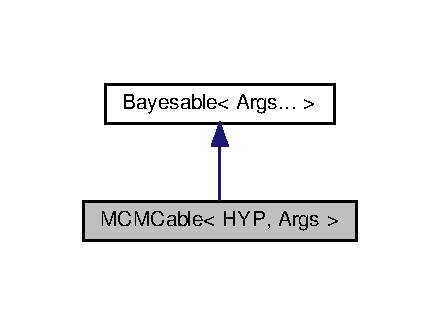
\includegraphics[width=211pt]{class_m_c_m_cable__inherit__graph}
\end{center}
\end{figure}


Collaboration diagram for M\+C\+M\+Cable$<$ H\+YP, Args $>$\+:\nopagebreak
\begin{figure}[H]
\begin{center}
\leavevmode
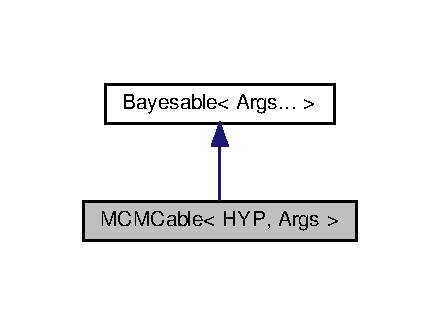
\includegraphics[width=211pt]{class_m_c_m_cable__coll__graph}
\end{center}
\end{figure}
\subsection*{Public Member Functions}
\begin{DoxyCompactItemize}
\item 
\hyperlink{class_m_c_m_cable_aac715433bffb674dd5809e7c1bc59ae5}{M\+C\+M\+Cable} ()
\item 
virtual std\+::pair$<$ H\+YP, double $>$ \hyperlink{class_m_c_m_cable_ab119a14256ab92c5c1e941f8492df830}{propose} () const =0
\item 
virtual H\+YP \hyperlink{class_m_c_m_cable_a220d6c4ca73e20441c14fa5bd3e090d3}{restart} () const =0
\item 
virtual bool \hyperlink{class_m_c_m_cable_aa73001ec3bb0cf0c618281dfa998f2f1}{operator==} (const H\+YP \&h) const =0
\end{DoxyCompactItemize}
\subsection*{Additional Inherited Members}


\subsection{Detailed Description}
\subsubsection*{template$<$typename H\+YP, typename ... Args$>$\newline
class M\+C\+M\+Cable$<$ H\+Y\+P, Args $>$}

\begin{DoxyAuthor}{Author}
steven piantadosi 
\end{DoxyAuthor}
\begin{DoxyDate}{Date}
03/02/20 
\end{DoxyDate}


\subsection{Constructor \& Destructor Documentation}
\mbox{\Hypertarget{class_m_c_m_cable_aac715433bffb674dd5809e7c1bc59ae5}\label{class_m_c_m_cable_aac715433bffb674dd5809e7c1bc59ae5}} 
\index{M\+C\+M\+Cable@{M\+C\+M\+Cable}!M\+C\+M\+Cable@{M\+C\+M\+Cable}}
\index{M\+C\+M\+Cable@{M\+C\+M\+Cable}!M\+C\+M\+Cable@{M\+C\+M\+Cable}}
\subsubsection{\texorpdfstring{M\+C\+M\+Cable()}{MCMCable()}}
{\footnotesize\ttfamily template$<$typename H\+YP, typename ... Args$>$ \\
\hyperlink{class_m_c_m_cable}{M\+C\+M\+Cable}$<$ H\+YP, Args $>$\+::\hyperlink{class_m_c_m_cable}{M\+C\+M\+Cable} (\begin{DoxyParamCaption}{ }\end{DoxyParamCaption})\hspace{0.3cm}{\ttfamily [inline]}}



\subsection{Member Function Documentation}
\mbox{\Hypertarget{class_m_c_m_cable_aa73001ec3bb0cf0c618281dfa998f2f1}\label{class_m_c_m_cable_aa73001ec3bb0cf0c618281dfa998f2f1}} 
\index{M\+C\+M\+Cable@{M\+C\+M\+Cable}!operator==@{operator==}}
\index{operator==@{operator==}!M\+C\+M\+Cable@{M\+C\+M\+Cable}}
\subsubsection{\texorpdfstring{operator==()}{operator==()}}
{\footnotesize\ttfamily template$<$typename H\+YP, typename ... Args$>$ \\
virtual bool \hyperlink{class_m_c_m_cable}{M\+C\+M\+Cable}$<$ H\+YP, Args $>$\+::operator== (\begin{DoxyParamCaption}\item[{const H\+YP \&}]{h }\end{DoxyParamCaption}) const\hspace{0.3cm}{\ttfamily [pure virtual]}}



Implemented in \hyperlink{class_grammar_hypothesis_a8a64510ebb2af15474bdae7169049c94}{Grammar\+Hypothesis$<$ H\+Y\+P, t\+\_\+datum, t\+\_\+data $>$}, \hyperlink{class_l_o_t_hypothesis_a26da0f250197d375b4ae2400815c3288}{L\+O\+T\+Hypothesis$<$ H\+Y\+P, T, t\+\_\+input, t\+\_\+output, \+\_\+t\+\_\+datum, \+\_\+t\+\_\+data $>$}, \hyperlink{class_l_o_t_hypothesis_a26da0f250197d375b4ae2400815c3288}{L\+O\+T\+Hypothesis$<$ Inner\+Hypothesis, Node, S, S $>$}, \hyperlink{class_l_o_t_hypothesis_a26da0f250197d375b4ae2400815c3288}{L\+O\+T\+Hypothesis$<$ My\+Hypothesis, Node, Object, bool $>$}, \hyperlink{class_l_o_t_hypothesis_a26da0f250197d375b4ae2400815c3288}{L\+O\+T\+Hypothesis$<$ My\+Hypothesis, Node, float, float, float, std\+::multiset$<$ float $>$ $>$}, \hyperlink{class_lexicon_a852faeedb6cd12e629e601ebcad41729}{Lexicon$<$ H\+Y\+P, T, t\+\_\+input, t\+\_\+output, t\+\_\+datum $>$}, and \hyperlink{class_lexicon_a852faeedb6cd12e629e601ebcad41729}{Lexicon$<$ My\+Hypothesis, Inner\+Hypothesis, S, S $>$}.

\mbox{\Hypertarget{class_m_c_m_cable_ab119a14256ab92c5c1e941f8492df830}\label{class_m_c_m_cable_ab119a14256ab92c5c1e941f8492df830}} 
\index{M\+C\+M\+Cable@{M\+C\+M\+Cable}!propose@{propose}}
\index{propose@{propose}!M\+C\+M\+Cable@{M\+C\+M\+Cable}}
\subsubsection{\texorpdfstring{propose()}{propose()}}
{\footnotesize\ttfamily template$<$typename H\+YP, typename ... Args$>$ \\
virtual std\+::pair$<$H\+YP,double$>$ \hyperlink{class_m_c_m_cable}{M\+C\+M\+Cable}$<$ H\+YP, Args $>$\+::propose (\begin{DoxyParamCaption}{ }\end{DoxyParamCaption}) const\hspace{0.3cm}{\ttfamily [pure virtual]}}



Implemented in \hyperlink{class_lexicon_a41a1955c8d373e85c3b926f161bf7e31}{Lexicon$<$ H\+Y\+P, T, t\+\_\+input, t\+\_\+output, t\+\_\+datum $>$}, \hyperlink{class_lexicon_a41a1955c8d373e85c3b926f161bf7e31}{Lexicon$<$ My\+Hypothesis, Inner\+Hypothesis, S, S $>$}, \hyperlink{class_grammar_hypothesis_a5b642e0ccd5c1cebdbd3f7dfdc81cfcf}{Grammar\+Hypothesis$<$ H\+Y\+P, t\+\_\+datum, t\+\_\+data $>$}, \hyperlink{class_l_o_t_hypothesis_ab6cff786f845f0001b497cc606d14c5a}{L\+O\+T\+Hypothesis$<$ H\+Y\+P, T, t\+\_\+input, t\+\_\+output, \+\_\+t\+\_\+datum, \+\_\+t\+\_\+data $>$}, \hyperlink{class_l_o_t_hypothesis_ab6cff786f845f0001b497cc606d14c5a}{L\+O\+T\+Hypothesis$<$ Inner\+Hypothesis, Node, S, S $>$}, \hyperlink{class_l_o_t_hypothesis_ab6cff786f845f0001b497cc606d14c5a}{L\+O\+T\+Hypothesis$<$ My\+Hypothesis, Node, Object, bool $>$}, and \hyperlink{class_l_o_t_hypothesis_ab6cff786f845f0001b497cc606d14c5a}{L\+O\+T\+Hypothesis$<$ My\+Hypothesis, Node, float, float, float, std\+::multiset$<$ float $>$ $>$}.

\mbox{\Hypertarget{class_m_c_m_cable_a220d6c4ca73e20441c14fa5bd3e090d3}\label{class_m_c_m_cable_a220d6c4ca73e20441c14fa5bd3e090d3}} 
\index{M\+C\+M\+Cable@{M\+C\+M\+Cable}!restart@{restart}}
\index{restart@{restart}!M\+C\+M\+Cable@{M\+C\+M\+Cable}}
\subsubsection{\texorpdfstring{restart()}{restart()}}
{\footnotesize\ttfamily template$<$typename H\+YP, typename ... Args$>$ \\
virtual H\+YP \hyperlink{class_m_c_m_cable}{M\+C\+M\+Cable}$<$ H\+YP, Args $>$\+::restart (\begin{DoxyParamCaption}{ }\end{DoxyParamCaption}) const\hspace{0.3cm}{\ttfamily [pure virtual]}}



Implemented in \hyperlink{class_lexicon_a4ffff098d0f444d3e9ec543bbd228595}{Lexicon$<$ H\+Y\+P, T, t\+\_\+input, t\+\_\+output, t\+\_\+datum $>$}, \hyperlink{class_lexicon_a4ffff098d0f444d3e9ec543bbd228595}{Lexicon$<$ My\+Hypothesis, Inner\+Hypothesis, S, S $>$}, \hyperlink{class_grammar_hypothesis_a8d0042f4858879ce2585df382ce78b0a}{Grammar\+Hypothesis$<$ H\+Y\+P, t\+\_\+datum, t\+\_\+data $>$}, \hyperlink{class_l_o_t_hypothesis_a1224617b004cc10b4c5b17b9da58fbd8}{L\+O\+T\+Hypothesis$<$ H\+Y\+P, T, t\+\_\+input, t\+\_\+output, \+\_\+t\+\_\+datum, \+\_\+t\+\_\+data $>$}, \hyperlink{class_l_o_t_hypothesis_a1224617b004cc10b4c5b17b9da58fbd8}{L\+O\+T\+Hypothesis$<$ Inner\+Hypothesis, Node, S, S $>$}, \hyperlink{class_l_o_t_hypothesis_a1224617b004cc10b4c5b17b9da58fbd8}{L\+O\+T\+Hypothesis$<$ My\+Hypothesis, Node, Object, bool $>$}, and \hyperlink{class_l_o_t_hypothesis_a1224617b004cc10b4c5b17b9da58fbd8}{L\+O\+T\+Hypothesis$<$ My\+Hypothesis, Node, float, float, float, std\+::multiset$<$ float $>$ $>$}.



The documentation for this class was generated from the following file\+:\begin{DoxyCompactItemize}
\item 
src/\+Hypotheses/\+Interfaces/\hyperlink{_m_c_m_cable_8h}{M\+C\+M\+Cable.\+h}\end{DoxyCompactItemize}

\hypertarget{class_m_c_m_c_chain}{}\section{M\+C\+M\+C\+Chain$<$ H\+YP, callback\+\_\+t $>$ Class Template Reference}
\label{class_m_c_m_c_chain}\index{M\+C\+M\+C\+Chain$<$ H\+Y\+P, callback\+\_\+t $>$@{M\+C\+M\+C\+Chain$<$ H\+Y\+P, callback\+\_\+t $>$}}


{\ttfamily \#include $<$M\+C\+M\+C\+Chain.\+h$>$}



Collaboration diagram for M\+C\+M\+C\+Chain$<$ H\+YP, callback\+\_\+t $>$\+:\nopagebreak
\begin{figure}[H]
\begin{center}
\leavevmode
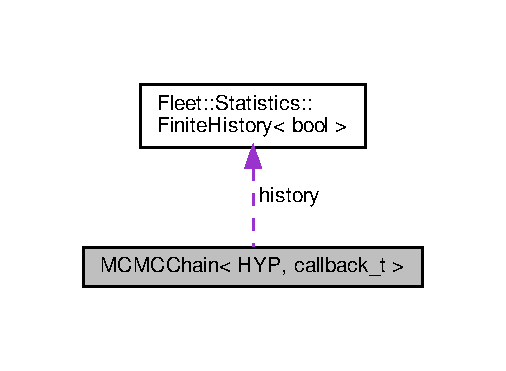
\includegraphics[width=243pt]{class_m_c_m_c_chain__coll__graph}
\end{center}
\end{figure}
\subsection*{Public Member Functions}
\begin{DoxyCompactItemize}
\item 
\hyperlink{class_m_c_m_c_chain_a60b036bec195eaa5a8081b2b8cc18eed}{M\+C\+M\+C\+Chain} (H\+YP \&h0, typename H\+Y\+P\+::t\+\_\+data $\ast$d, callback\+\_\+t \&cb)
\item 
\hyperlink{class_m_c_m_c_chain_ac75dc993bdc19b193ef6f128d62f8208}{M\+C\+M\+C\+Chain} (H\+YP \&\&h0, typename H\+Y\+P\+::t\+\_\+data $\ast$d, callback\+\_\+t \&cb)
\item 
\hyperlink{class_m_c_m_c_chain_a60ef818850d6836a21169d6e9bc14221}{M\+C\+M\+C\+Chain} (H\+YP \&h0, typename H\+Y\+P\+::t\+\_\+data $\ast$d, callback\+\_\+t $\ast$cb=nullptr)
\item 
\hyperlink{class_m_c_m_c_chain_a02d18b967945d40689cbe327bfd453e3}{M\+C\+M\+C\+Chain} (H\+YP \&\&h0, typename H\+Y\+P\+::t\+\_\+data $\ast$d, callback\+\_\+t $\ast$cb=nullptr)
\item 
\hyperlink{class_m_c_m_c_chain_a3942ff362dcc0bdfdad296f95048f14e}{M\+C\+M\+C\+Chain} (const \hyperlink{class_m_c_m_c_chain}{M\+C\+M\+C\+Chain} \&m)
\item 
\hyperlink{class_m_c_m_c_chain_a2db84c6b92af066b34eedd257d800417}{M\+C\+M\+C\+Chain} (\hyperlink{class_m_c_m_c_chain}{M\+C\+M\+C\+Chain} \&\&m)
\item 
virtual \hyperlink{class_m_c_m_c_chain_ad19438dd99bdba43b5175705e2bef156}{$\sim$\+M\+C\+M\+C\+Chain} ()
\item 
H\+YP \& \hyperlink{class_m_c_m_c_chain_ae76c66b5bcbc02df926e5f9a91acff17}{get\+Current} ()
\item 
void \hyperlink{class_m_c_m_c_chain_a4214114e0ef4adcd4badfe1440693190}{run\+On\+Current} ()
\item 
const H\+YP \& \hyperlink{class_m_c_m_c_chain_aa5c2bf3cae9a5959cab43e04b1201ed2}{get\+Max} ()
\item 
void \hyperlink{class_m_c_m_c_chain_aef30134b1915b8b494040771480d6b80}{run} (\hyperlink{struct_control}{Control} ctl)
\item 
void \hyperlink{class_m_c_m_c_chain_ae59e07a79da1bf56b01429efcb9fb312}{run} ()
\item 
double \hyperlink{class_m_c_m_c_chain_a4b2b8b51e5ba868bca024f2be737e4c6}{acceptance\+\_\+ratio} ()
\item 
double \hyperlink{class_m_c_m_c_chain_a9adc3d08662ad7035cc9d9d75a1fc5a6}{at\+\_\+temperature} (double t)
\end{DoxyCompactItemize}
\subsection*{Public Attributes}
\begin{DoxyCompactItemize}
\item 
H\+YP \hyperlink{class_m_c_m_c_chain_ab0c3b31e96d1f703bb8cf55c0575b4bd}{current}
\item 
std\+::mutex \hyperlink{class_m_c_m_c_chain_a42c355121fce0476426a49d5498c38a1}{current\+\_\+mutex}
\item 
H\+Y\+P\+::t\+\_\+data $\ast$ \hyperlink{class_m_c_m_c_chain_a62ffa9a3d173a79c82f09174b58aebaf}{data}
\item 
H\+YP \hyperlink{class_m_c_m_c_chain_a966ec00d236d4df6c477c6fd5575fd87}{themax}
\item 
callback\+\_\+t $\ast$ \hyperlink{class_m_c_m_c_chain_aa7a4a0d46ae2d9818c2f076f839badd7}{callback}
\item 
bool \hyperlink{class_m_c_m_c_chain_ad51e645f9de68d3f008b62ada6375099}{returnmax}
\item 
unsigned long \hyperlink{class_m_c_m_c_chain_a0d3ac649b04077cd0ffea236df560c91}{samples}
\item 
unsigned long \hyperlink{class_m_c_m_c_chain_aec2cdd6a3e25447c7f34e31d0d98dbcb}{proposals}
\item 
unsigned long \hyperlink{class_m_c_m_c_chain_ae1597e42074b2efb93ace3e40f1f7a45}{acceptances}
\item 
unsigned long \hyperlink{class_m_c_m_c_chain_aeac1cd63d13c397ba01cca35b605b786}{steps\+\_\+since\+\_\+improvement}
\item 
std\+::atomic$<$ double $>$ \hyperlink{class_m_c_m_c_chain_a7173287e1c0e681a9912a84c87320ece}{temperature}
\item 
\hyperlink{class_fleet_1_1_statistics_1_1_finite_history}{Fleet\+::\+Statistics\+::\+Finite\+History}$<$ bool $>$ \hyperlink{class_m_c_m_c_chain_a2595f417e0c9cc847ac1dd70ed8b0763}{history}
\end{DoxyCompactItemize}


\subsection{Constructor \& Destructor Documentation}
\mbox{\Hypertarget{class_m_c_m_c_chain_a60b036bec195eaa5a8081b2b8cc18eed}\label{class_m_c_m_c_chain_a60b036bec195eaa5a8081b2b8cc18eed}} 
\index{M\+C\+M\+C\+Chain@{M\+C\+M\+C\+Chain}!M\+C\+M\+C\+Chain@{M\+C\+M\+C\+Chain}}
\index{M\+C\+M\+C\+Chain@{M\+C\+M\+C\+Chain}!M\+C\+M\+C\+Chain@{M\+C\+M\+C\+Chain}}
\subsubsection{\texorpdfstring{M\+C\+M\+C\+Chain()}{MCMCChain()}\hspace{0.1cm}{\footnotesize\ttfamily [1/6]}}
{\footnotesize\ttfamily template$<$typename H\+YP , typename callback\+\_\+t $>$ \\
\hyperlink{class_m_c_m_c_chain}{M\+C\+M\+C\+Chain}$<$ H\+YP, callback\+\_\+t $>$\+::\hyperlink{class_m_c_m_c_chain}{M\+C\+M\+C\+Chain} (\begin{DoxyParamCaption}\item[{H\+YP \&}]{h0,  }\item[{typename H\+Y\+P\+::t\+\_\+data $\ast$}]{d,  }\item[{callback\+\_\+t \&}]{cb }\end{DoxyParamCaption})\hspace{0.3cm}{\ttfamily [inline]}}

\mbox{\Hypertarget{class_m_c_m_c_chain_ac75dc993bdc19b193ef6f128d62f8208}\label{class_m_c_m_c_chain_ac75dc993bdc19b193ef6f128d62f8208}} 
\index{M\+C\+M\+C\+Chain@{M\+C\+M\+C\+Chain}!M\+C\+M\+C\+Chain@{M\+C\+M\+C\+Chain}}
\index{M\+C\+M\+C\+Chain@{M\+C\+M\+C\+Chain}!M\+C\+M\+C\+Chain@{M\+C\+M\+C\+Chain}}
\subsubsection{\texorpdfstring{M\+C\+M\+C\+Chain()}{MCMCChain()}\hspace{0.1cm}{\footnotesize\ttfamily [2/6]}}
{\footnotesize\ttfamily template$<$typename H\+YP , typename callback\+\_\+t $>$ \\
\hyperlink{class_m_c_m_c_chain}{M\+C\+M\+C\+Chain}$<$ H\+YP, callback\+\_\+t $>$\+::\hyperlink{class_m_c_m_c_chain}{M\+C\+M\+C\+Chain} (\begin{DoxyParamCaption}\item[{H\+YP \&\&}]{h0,  }\item[{typename H\+Y\+P\+::t\+\_\+data $\ast$}]{d,  }\item[{callback\+\_\+t \&}]{cb }\end{DoxyParamCaption})\hspace{0.3cm}{\ttfamily [inline]}}

\mbox{\Hypertarget{class_m_c_m_c_chain_a60ef818850d6836a21169d6e9bc14221}\label{class_m_c_m_c_chain_a60ef818850d6836a21169d6e9bc14221}} 
\index{M\+C\+M\+C\+Chain@{M\+C\+M\+C\+Chain}!M\+C\+M\+C\+Chain@{M\+C\+M\+C\+Chain}}
\index{M\+C\+M\+C\+Chain@{M\+C\+M\+C\+Chain}!M\+C\+M\+C\+Chain@{M\+C\+M\+C\+Chain}}
\subsubsection{\texorpdfstring{M\+C\+M\+C\+Chain()}{MCMCChain()}\hspace{0.1cm}{\footnotesize\ttfamily [3/6]}}
{\footnotesize\ttfamily template$<$typename H\+YP , typename callback\+\_\+t $>$ \\
\hyperlink{class_m_c_m_c_chain}{M\+C\+M\+C\+Chain}$<$ H\+YP, callback\+\_\+t $>$\+::\hyperlink{class_m_c_m_c_chain}{M\+C\+M\+C\+Chain} (\begin{DoxyParamCaption}\item[{H\+YP \&}]{h0,  }\item[{typename H\+Y\+P\+::t\+\_\+data $\ast$}]{d,  }\item[{callback\+\_\+t $\ast$}]{cb = {\ttfamily nullptr} }\end{DoxyParamCaption})\hspace{0.3cm}{\ttfamily [inline]}}

\mbox{\Hypertarget{class_m_c_m_c_chain_a02d18b967945d40689cbe327bfd453e3}\label{class_m_c_m_c_chain_a02d18b967945d40689cbe327bfd453e3}} 
\index{M\+C\+M\+C\+Chain@{M\+C\+M\+C\+Chain}!M\+C\+M\+C\+Chain@{M\+C\+M\+C\+Chain}}
\index{M\+C\+M\+C\+Chain@{M\+C\+M\+C\+Chain}!M\+C\+M\+C\+Chain@{M\+C\+M\+C\+Chain}}
\subsubsection{\texorpdfstring{M\+C\+M\+C\+Chain()}{MCMCChain()}\hspace{0.1cm}{\footnotesize\ttfamily [4/6]}}
{\footnotesize\ttfamily template$<$typename H\+YP , typename callback\+\_\+t $>$ \\
\hyperlink{class_m_c_m_c_chain}{M\+C\+M\+C\+Chain}$<$ H\+YP, callback\+\_\+t $>$\+::\hyperlink{class_m_c_m_c_chain}{M\+C\+M\+C\+Chain} (\begin{DoxyParamCaption}\item[{H\+YP \&\&}]{h0,  }\item[{typename H\+Y\+P\+::t\+\_\+data $\ast$}]{d,  }\item[{callback\+\_\+t $\ast$}]{cb = {\ttfamily nullptr} }\end{DoxyParamCaption})\hspace{0.3cm}{\ttfamily [inline]}}

\mbox{\Hypertarget{class_m_c_m_c_chain_a3942ff362dcc0bdfdad296f95048f14e}\label{class_m_c_m_c_chain_a3942ff362dcc0bdfdad296f95048f14e}} 
\index{M\+C\+M\+C\+Chain@{M\+C\+M\+C\+Chain}!M\+C\+M\+C\+Chain@{M\+C\+M\+C\+Chain}}
\index{M\+C\+M\+C\+Chain@{M\+C\+M\+C\+Chain}!M\+C\+M\+C\+Chain@{M\+C\+M\+C\+Chain}}
\subsubsection{\texorpdfstring{M\+C\+M\+C\+Chain()}{MCMCChain()}\hspace{0.1cm}{\footnotesize\ttfamily [5/6]}}
{\footnotesize\ttfamily template$<$typename H\+YP , typename callback\+\_\+t $>$ \\
\hyperlink{class_m_c_m_c_chain}{M\+C\+M\+C\+Chain}$<$ H\+YP, callback\+\_\+t $>$\+::\hyperlink{class_m_c_m_c_chain}{M\+C\+M\+C\+Chain} (\begin{DoxyParamCaption}\item[{const \hyperlink{class_m_c_m_c_chain}{M\+C\+M\+C\+Chain}$<$ H\+YP, callback\+\_\+t $>$ \&}]{m }\end{DoxyParamCaption})\hspace{0.3cm}{\ttfamily [inline]}}

\mbox{\Hypertarget{class_m_c_m_c_chain_a2db84c6b92af066b34eedd257d800417}\label{class_m_c_m_c_chain_a2db84c6b92af066b34eedd257d800417}} 
\index{M\+C\+M\+C\+Chain@{M\+C\+M\+C\+Chain}!M\+C\+M\+C\+Chain@{M\+C\+M\+C\+Chain}}
\index{M\+C\+M\+C\+Chain@{M\+C\+M\+C\+Chain}!M\+C\+M\+C\+Chain@{M\+C\+M\+C\+Chain}}
\subsubsection{\texorpdfstring{M\+C\+M\+C\+Chain()}{MCMCChain()}\hspace{0.1cm}{\footnotesize\ttfamily [6/6]}}
{\footnotesize\ttfamily template$<$typename H\+YP , typename callback\+\_\+t $>$ \\
\hyperlink{class_m_c_m_c_chain}{M\+C\+M\+C\+Chain}$<$ H\+YP, callback\+\_\+t $>$\+::\hyperlink{class_m_c_m_c_chain}{M\+C\+M\+C\+Chain} (\begin{DoxyParamCaption}\item[{\hyperlink{class_m_c_m_c_chain}{M\+C\+M\+C\+Chain}$<$ H\+YP, callback\+\_\+t $>$ \&\&}]{m }\end{DoxyParamCaption})\hspace{0.3cm}{\ttfamily [inline]}}

\mbox{\Hypertarget{class_m_c_m_c_chain_ad19438dd99bdba43b5175705e2bef156}\label{class_m_c_m_c_chain_ad19438dd99bdba43b5175705e2bef156}} 
\index{M\+C\+M\+C\+Chain@{M\+C\+M\+C\+Chain}!````~M\+C\+M\+C\+Chain@{$\sim$\+M\+C\+M\+C\+Chain}}
\index{````~M\+C\+M\+C\+Chain@{$\sim$\+M\+C\+M\+C\+Chain}!M\+C\+M\+C\+Chain@{M\+C\+M\+C\+Chain}}
\subsubsection{\texorpdfstring{$\sim$\+M\+C\+M\+C\+Chain()}{~MCMCChain()}}
{\footnotesize\ttfamily template$<$typename H\+YP , typename callback\+\_\+t $>$ \\
virtual \hyperlink{class_m_c_m_c_chain}{M\+C\+M\+C\+Chain}$<$ H\+YP, callback\+\_\+t $>$\+::$\sim$\hyperlink{class_m_c_m_c_chain}{M\+C\+M\+C\+Chain} (\begin{DoxyParamCaption}{ }\end{DoxyParamCaption})\hspace{0.3cm}{\ttfamily [inline]}, {\ttfamily [virtual]}}



\subsection{Member Function Documentation}
\mbox{\Hypertarget{class_m_c_m_c_chain_a4b2b8b51e5ba868bca024f2be737e4c6}\label{class_m_c_m_c_chain_a4b2b8b51e5ba868bca024f2be737e4c6}} 
\index{M\+C\+M\+C\+Chain@{M\+C\+M\+C\+Chain}!acceptance\+\_\+ratio@{acceptance\+\_\+ratio}}
\index{acceptance\+\_\+ratio@{acceptance\+\_\+ratio}!M\+C\+M\+C\+Chain@{M\+C\+M\+C\+Chain}}
\subsubsection{\texorpdfstring{acceptance\+\_\+ratio()}{acceptance\_ratio()}}
{\footnotesize\ttfamily template$<$typename H\+YP , typename callback\+\_\+t $>$ \\
double \hyperlink{class_m_c_m_c_chain}{M\+C\+M\+C\+Chain}$<$ H\+YP, callback\+\_\+t $>$\+::acceptance\+\_\+ratio (\begin{DoxyParamCaption}{ }\end{DoxyParamCaption})\hspace{0.3cm}{\ttfamily [inline]}}

Get my acceptance ratio \begin{DoxyReturn}{Returns}

\end{DoxyReturn}
\mbox{\Hypertarget{class_m_c_m_c_chain_a9adc3d08662ad7035cc9d9d75a1fc5a6}\label{class_m_c_m_c_chain_a9adc3d08662ad7035cc9d9d75a1fc5a6}} 
\index{M\+C\+M\+C\+Chain@{M\+C\+M\+C\+Chain}!at\+\_\+temperature@{at\+\_\+temperature}}
\index{at\+\_\+temperature@{at\+\_\+temperature}!M\+C\+M\+C\+Chain@{M\+C\+M\+C\+Chain}}
\subsubsection{\texorpdfstring{at\+\_\+temperature()}{at\_temperature()}}
{\footnotesize\ttfamily template$<$typename H\+YP , typename callback\+\_\+t $>$ \\
double \hyperlink{class_m_c_m_c_chain}{M\+C\+M\+C\+Chain}$<$ H\+YP, callback\+\_\+t $>$\+::at\+\_\+temperature (\begin{DoxyParamCaption}\item[{double}]{t }\end{DoxyParamCaption})\hspace{0.3cm}{\ttfamily [inline]}}

Return my current posterior at a given temperature t 
\begin{DoxyParams}{Parameters}
{\em t} & \\
\hline
\end{DoxyParams}
\begin{DoxyReturn}{Returns}

\end{DoxyReturn}
\mbox{\Hypertarget{class_m_c_m_c_chain_ae76c66b5bcbc02df926e5f9a91acff17}\label{class_m_c_m_c_chain_ae76c66b5bcbc02df926e5f9a91acff17}} 
\index{M\+C\+M\+C\+Chain@{M\+C\+M\+C\+Chain}!get\+Current@{get\+Current}}
\index{get\+Current@{get\+Current}!M\+C\+M\+C\+Chain@{M\+C\+M\+C\+Chain}}
\subsubsection{\texorpdfstring{get\+Current()}{getCurrent()}}
{\footnotesize\ttfamily template$<$typename H\+YP , typename callback\+\_\+t $>$ \\
H\+YP\& \hyperlink{class_m_c_m_c_chain}{M\+C\+M\+C\+Chain}$<$ H\+YP, callback\+\_\+t $>$\+::get\+Current (\begin{DoxyParamCaption}{ }\end{DoxyParamCaption})\hspace{0.3cm}{\ttfamily [inline]}}

get a reference to the current value \begin{DoxyReturn}{Returns}

\end{DoxyReturn}
\mbox{\Hypertarget{class_m_c_m_c_chain_aa5c2bf3cae9a5959cab43e04b1201ed2}\label{class_m_c_m_c_chain_aa5c2bf3cae9a5959cab43e04b1201ed2}} 
\index{M\+C\+M\+C\+Chain@{M\+C\+M\+C\+Chain}!get\+Max@{get\+Max}}
\index{get\+Max@{get\+Max}!M\+C\+M\+C\+Chain@{M\+C\+M\+C\+Chain}}
\subsubsection{\texorpdfstring{get\+Max()}{getMax()}}
{\footnotesize\ttfamily template$<$typename H\+YP , typename callback\+\_\+t $>$ \\
const H\+YP\& \hyperlink{class_m_c_m_c_chain}{M\+C\+M\+C\+Chain}$<$ H\+YP, callback\+\_\+t $>$\+::get\+Max (\begin{DoxyParamCaption}{ }\end{DoxyParamCaption})\hspace{0.3cm}{\ttfamily [inline]}}

\mbox{\Hypertarget{class_m_c_m_c_chain_aef30134b1915b8b494040771480d6b80}\label{class_m_c_m_c_chain_aef30134b1915b8b494040771480d6b80}} 
\index{M\+C\+M\+C\+Chain@{M\+C\+M\+C\+Chain}!run@{run}}
\index{run@{run}!M\+C\+M\+C\+Chain@{M\+C\+M\+C\+Chain}}
\subsubsection{\texorpdfstring{run()}{run()}\hspace{0.1cm}{\footnotesize\ttfamily [1/2]}}
{\footnotesize\ttfamily template$<$typename H\+YP , typename callback\+\_\+t $>$ \\
void \hyperlink{class_m_c_m_c_chain}{M\+C\+M\+C\+Chain}$<$ H\+YP, callback\+\_\+t $>$\+::run (\begin{DoxyParamCaption}\item[{\hyperlink{struct_control}{Control}}]{ctl }\end{DoxyParamCaption})\hspace{0.3cm}{\ttfamily [inline]}}

Run M\+C\+MC according to the control parameters passed in. N\+O\+TE\+: ctl cannot be passed by reference. 
\begin{DoxyParams}{Parameters}
{\em ctl} & \\
\hline
\end{DoxyParams}
\mbox{\Hypertarget{class_m_c_m_c_chain_ae59e07a79da1bf56b01429efcb9fb312}\label{class_m_c_m_c_chain_ae59e07a79da1bf56b01429efcb9fb312}} 
\index{M\+C\+M\+C\+Chain@{M\+C\+M\+C\+Chain}!run@{run}}
\index{run@{run}!M\+C\+M\+C\+Chain@{M\+C\+M\+C\+Chain}}
\subsubsection{\texorpdfstring{run()}{run()}\hspace{0.1cm}{\footnotesize\ttfamily [2/2]}}
{\footnotesize\ttfamily template$<$typename H\+YP , typename callback\+\_\+t $>$ \\
void \hyperlink{class_m_c_m_c_chain}{M\+C\+M\+C\+Chain}$<$ H\+YP, callback\+\_\+t $>$\+::run (\begin{DoxyParamCaption}{ }\end{DoxyParamCaption})\hspace{0.3cm}{\ttfamily [inline]}}

Run forever\mbox{\Hypertarget{class_m_c_m_c_chain_a4214114e0ef4adcd4badfe1440693190}\label{class_m_c_m_c_chain_a4214114e0ef4adcd4badfe1440693190}} 
\index{M\+C\+M\+C\+Chain@{M\+C\+M\+C\+Chain}!run\+On\+Current@{run\+On\+Current}}
\index{run\+On\+Current@{run\+On\+Current}!M\+C\+M\+C\+Chain@{M\+C\+M\+C\+Chain}}
\subsubsection{\texorpdfstring{run\+On\+Current()}{runOnCurrent()}}
{\footnotesize\ttfamily template$<$typename H\+YP , typename callback\+\_\+t $>$ \\
void \hyperlink{class_m_c_m_c_chain}{M\+C\+M\+C\+Chain}$<$ H\+YP, callback\+\_\+t $>$\+::run\+On\+Current (\begin{DoxyParamCaption}{ }\end{DoxyParamCaption})\hspace{0.3cm}{\ttfamily [inline]}}

This is called by the constructor to compute the posterior and callback for an initial h0

\subsection{Member Data Documentation}
\mbox{\Hypertarget{class_m_c_m_c_chain_ae1597e42074b2efb93ace3e40f1f7a45}\label{class_m_c_m_c_chain_ae1597e42074b2efb93ace3e40f1f7a45}} 
\index{M\+C\+M\+C\+Chain@{M\+C\+M\+C\+Chain}!acceptances@{acceptances}}
\index{acceptances@{acceptances}!M\+C\+M\+C\+Chain@{M\+C\+M\+C\+Chain}}
\subsubsection{\texorpdfstring{acceptances}{acceptances}}
{\footnotesize\ttfamily template$<$typename H\+YP , typename callback\+\_\+t $>$ \\
unsigned long \hyperlink{class_m_c_m_c_chain}{M\+C\+M\+C\+Chain}$<$ H\+YP, callback\+\_\+t $>$\+::acceptances}

\mbox{\Hypertarget{class_m_c_m_c_chain_aa7a4a0d46ae2d9818c2f076f839badd7}\label{class_m_c_m_c_chain_aa7a4a0d46ae2d9818c2f076f839badd7}} 
\index{M\+C\+M\+C\+Chain@{M\+C\+M\+C\+Chain}!callback@{callback}}
\index{callback@{callback}!M\+C\+M\+C\+Chain@{M\+C\+M\+C\+Chain}}
\subsubsection{\texorpdfstring{callback}{callback}}
{\footnotesize\ttfamily template$<$typename H\+YP , typename callback\+\_\+t $>$ \\
callback\+\_\+t$\ast$ \hyperlink{class_m_c_m_c_chain}{M\+C\+M\+C\+Chain}$<$ H\+YP, callback\+\_\+t $>$\+::callback}

\mbox{\Hypertarget{class_m_c_m_c_chain_ab0c3b31e96d1f703bb8cf55c0575b4bd}\label{class_m_c_m_c_chain_ab0c3b31e96d1f703bb8cf55c0575b4bd}} 
\index{M\+C\+M\+C\+Chain@{M\+C\+M\+C\+Chain}!current@{current}}
\index{current@{current}!M\+C\+M\+C\+Chain@{M\+C\+M\+C\+Chain}}
\subsubsection{\texorpdfstring{current}{current}}
{\footnotesize\ttfamily template$<$typename H\+YP , typename callback\+\_\+t $>$ \\
H\+YP \hyperlink{class_m_c_m_c_chain}{M\+C\+M\+C\+Chain}$<$ H\+YP, callback\+\_\+t $>$\+::current}

\mbox{\Hypertarget{class_m_c_m_c_chain_a42c355121fce0476426a49d5498c38a1}\label{class_m_c_m_c_chain_a42c355121fce0476426a49d5498c38a1}} 
\index{M\+C\+M\+C\+Chain@{M\+C\+M\+C\+Chain}!current\+\_\+mutex@{current\+\_\+mutex}}
\index{current\+\_\+mutex@{current\+\_\+mutex}!M\+C\+M\+C\+Chain@{M\+C\+M\+C\+Chain}}
\subsubsection{\texorpdfstring{current\+\_\+mutex}{current\_mutex}}
{\footnotesize\ttfamily template$<$typename H\+YP , typename callback\+\_\+t $>$ \\
std\+::mutex \hyperlink{class_m_c_m_c_chain}{M\+C\+M\+C\+Chain}$<$ H\+YP, callback\+\_\+t $>$\+::current\+\_\+mutex\hspace{0.3cm}{\ttfamily [mutable]}}

\mbox{\Hypertarget{class_m_c_m_c_chain_a62ffa9a3d173a79c82f09174b58aebaf}\label{class_m_c_m_c_chain_a62ffa9a3d173a79c82f09174b58aebaf}} 
\index{M\+C\+M\+C\+Chain@{M\+C\+M\+C\+Chain}!data@{data}}
\index{data@{data}!M\+C\+M\+C\+Chain@{M\+C\+M\+C\+Chain}}
\subsubsection{\texorpdfstring{data}{data}}
{\footnotesize\ttfamily template$<$typename H\+YP , typename callback\+\_\+t $>$ \\
H\+Y\+P\+::t\+\_\+data$\ast$ \hyperlink{class_m_c_m_c_chain}{M\+C\+M\+C\+Chain}$<$ H\+YP, callback\+\_\+t $>$\+::data}

\mbox{\Hypertarget{class_m_c_m_c_chain_a2595f417e0c9cc847ac1dd70ed8b0763}\label{class_m_c_m_c_chain_a2595f417e0c9cc847ac1dd70ed8b0763}} 
\index{M\+C\+M\+C\+Chain@{M\+C\+M\+C\+Chain}!history@{history}}
\index{history@{history}!M\+C\+M\+C\+Chain@{M\+C\+M\+C\+Chain}}
\subsubsection{\texorpdfstring{history}{history}}
{\footnotesize\ttfamily template$<$typename H\+YP , typename callback\+\_\+t $>$ \\
\hyperlink{class_fleet_1_1_statistics_1_1_finite_history}{Fleet\+::\+Statistics\+::\+Finite\+History}$<$bool$>$ \hyperlink{class_m_c_m_c_chain}{M\+C\+M\+C\+Chain}$<$ H\+YP, callback\+\_\+t $>$\+::history}

\mbox{\Hypertarget{class_m_c_m_c_chain_aec2cdd6a3e25447c7f34e31d0d98dbcb}\label{class_m_c_m_c_chain_aec2cdd6a3e25447c7f34e31d0d98dbcb}} 
\index{M\+C\+M\+C\+Chain@{M\+C\+M\+C\+Chain}!proposals@{proposals}}
\index{proposals@{proposals}!M\+C\+M\+C\+Chain@{M\+C\+M\+C\+Chain}}
\subsubsection{\texorpdfstring{proposals}{proposals}}
{\footnotesize\ttfamily template$<$typename H\+YP , typename callback\+\_\+t $>$ \\
unsigned long \hyperlink{class_m_c_m_c_chain}{M\+C\+M\+C\+Chain}$<$ H\+YP, callback\+\_\+t $>$\+::proposals}

\mbox{\Hypertarget{class_m_c_m_c_chain_ad51e645f9de68d3f008b62ada6375099}\label{class_m_c_m_c_chain_ad51e645f9de68d3f008b62ada6375099}} 
\index{M\+C\+M\+C\+Chain@{M\+C\+M\+C\+Chain}!returnmax@{returnmax}}
\index{returnmax@{returnmax}!M\+C\+M\+C\+Chain@{M\+C\+M\+C\+Chain}}
\subsubsection{\texorpdfstring{returnmax}{returnmax}}
{\footnotesize\ttfamily template$<$typename H\+YP , typename callback\+\_\+t $>$ \\
bool \hyperlink{class_m_c_m_c_chain}{M\+C\+M\+C\+Chain}$<$ H\+YP, callback\+\_\+t $>$\+::returnmax}

\mbox{\Hypertarget{class_m_c_m_c_chain_a0d3ac649b04077cd0ffea236df560c91}\label{class_m_c_m_c_chain_a0d3ac649b04077cd0ffea236df560c91}} 
\index{M\+C\+M\+C\+Chain@{M\+C\+M\+C\+Chain}!samples@{samples}}
\index{samples@{samples}!M\+C\+M\+C\+Chain@{M\+C\+M\+C\+Chain}}
\subsubsection{\texorpdfstring{samples}{samples}}
{\footnotesize\ttfamily template$<$typename H\+YP , typename callback\+\_\+t $>$ \\
unsigned long \hyperlink{class_m_c_m_c_chain}{M\+C\+M\+C\+Chain}$<$ H\+YP, callback\+\_\+t $>$\+::samples}

\mbox{\Hypertarget{class_m_c_m_c_chain_aeac1cd63d13c397ba01cca35b605b786}\label{class_m_c_m_c_chain_aeac1cd63d13c397ba01cca35b605b786}} 
\index{M\+C\+M\+C\+Chain@{M\+C\+M\+C\+Chain}!steps\+\_\+since\+\_\+improvement@{steps\+\_\+since\+\_\+improvement}}
\index{steps\+\_\+since\+\_\+improvement@{steps\+\_\+since\+\_\+improvement}!M\+C\+M\+C\+Chain@{M\+C\+M\+C\+Chain}}
\subsubsection{\texorpdfstring{steps\+\_\+since\+\_\+improvement}{steps\_since\_improvement}}
{\footnotesize\ttfamily template$<$typename H\+YP , typename callback\+\_\+t $>$ \\
unsigned long \hyperlink{class_m_c_m_c_chain}{M\+C\+M\+C\+Chain}$<$ H\+YP, callback\+\_\+t $>$\+::steps\+\_\+since\+\_\+improvement}

\mbox{\Hypertarget{class_m_c_m_c_chain_a7173287e1c0e681a9912a84c87320ece}\label{class_m_c_m_c_chain_a7173287e1c0e681a9912a84c87320ece}} 
\index{M\+C\+M\+C\+Chain@{M\+C\+M\+C\+Chain}!temperature@{temperature}}
\index{temperature@{temperature}!M\+C\+M\+C\+Chain@{M\+C\+M\+C\+Chain}}
\subsubsection{\texorpdfstring{temperature}{temperature}}
{\footnotesize\ttfamily template$<$typename H\+YP , typename callback\+\_\+t $>$ \\
std\+::atomic$<$double$>$ \hyperlink{class_m_c_m_c_chain}{M\+C\+M\+C\+Chain}$<$ H\+YP, callback\+\_\+t $>$\+::temperature}

\mbox{\Hypertarget{class_m_c_m_c_chain_a966ec00d236d4df6c477c6fd5575fd87}\label{class_m_c_m_c_chain_a966ec00d236d4df6c477c6fd5575fd87}} 
\index{M\+C\+M\+C\+Chain@{M\+C\+M\+C\+Chain}!themax@{themax}}
\index{themax@{themax}!M\+C\+M\+C\+Chain@{M\+C\+M\+C\+Chain}}
\subsubsection{\texorpdfstring{themax}{themax}}
{\footnotesize\ttfamily template$<$typename H\+YP , typename callback\+\_\+t $>$ \\
H\+YP \hyperlink{class_m_c_m_c_chain}{M\+C\+M\+C\+Chain}$<$ H\+YP, callback\+\_\+t $>$\+::themax}



The documentation for this class was generated from the following file\+:\begin{DoxyCompactItemize}
\item 
src/\+Inference/\hyperlink{_m_c_m_c_chain_8h}{M\+C\+M\+C\+Chain.\+h}\end{DoxyCompactItemize}

\hypertarget{class_m_c_t_s_node}{}\section{M\+C\+T\+S\+Node$<$ M, H\+YP $>$ Class Template Reference}
\label{class_m_c_t_s_node}\index{M\+C\+T\+S\+Node$<$ M, H\+Y\+P $>$@{M\+C\+T\+S\+Node$<$ M, H\+Y\+P $>$}}


{\ttfamily \#include $<$M\+C\+T\+S.\+h$>$}



Collaboration diagram for M\+C\+T\+S\+Node$<$ M, H\+YP $>$\+:
\nopagebreak
\begin{figure}[H]
\begin{center}
\leavevmode
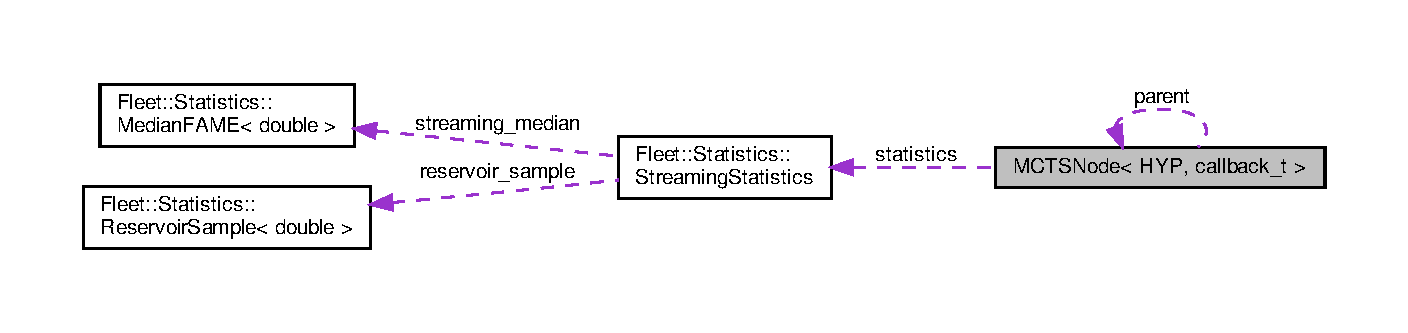
\includegraphics[width=350pt]{class_m_c_t_s_node__coll__graph}
\end{center}
\end{figure}
\subsection*{Public Member Functions}
\begin{DoxyCompactItemize}
\item 
\hyperlink{class_m_c_t_s_node_a94e679ddbb9f4eeaaa45b6214889f47c}{M\+C\+T\+S\+Node} (M $\ast$par, H\+YP \&v)
\item 
\hyperlink{class_m_c_t_s_node_a944daa7d3d710b6e8000dc8dc076c674}{M\+C\+T\+S\+Node} (double ex, H\+YP \&h0, typename H\+Y\+P\+::t\+\_\+data $\ast$d)
\item 
\hyperlink{class_m_c_t_s_node_aaa84f65b021fd06667185b4b9c5931e6}{M\+C\+T\+S\+Node} (const \hyperlink{class_m_c_t_s_node}{M\+C\+T\+S\+Node} \&m)=delete
\item 
\hyperlink{class_m_c_t_s_node_acf0c6f2110d0acb7dd1a281d3138056d}{M\+C\+T\+S\+Node} (\hyperlink{class_m_c_t_s_node}{M\+C\+T\+S\+Node} \&\&m)
\item 
virtual void \hyperlink{class_m_c_t_s_node_a9b98535db702f0e9ee221615bd658214}{playout} ()=0
\begin{DoxyCompactList}\small\item\em This must get overwritten when we want to use a M\+C\+TS node. \end{DoxyCompactList}\item 
size\+\_\+t \hyperlink{class_m_c_t_s_node_a7996e64e69b1fc705c4e21b4a6e41c39}{size} () const
\item 
void \hyperlink{class_m_c_t_s_node_aadbe8d42f6761eb3e4f28fb9157a873d}{initialize} ()
\item 
void \hyperlink{class_m_c_t_s_node_ab4d95f5a7a753b39d30771b4e385a934}{print} (std\+::ostream \&o, const int depth, const bool sort) const
\item 
void \hyperlink{class_m_c_t_s_node_ad82ca09e761b18033a2418c3f564151f}{print} (const bool sort=true) const
\item 
void \hyperlink{class_m_c_t_s_node_a258317ddcd07a57a34a9a2eeec6f10b9}{printerr} (const bool sort=true) const
\item 
void \hyperlink{class_m_c_t_s_node_ae0d17485c455b8d7e4fa9ee1a179d631}{print} (const char $\ast$filename, const bool sort=true) const
\item 
double \hyperlink{class_m_c_t_s_node_a1a051c22b8821704a10bf33dbd426c4d}{score} () const
\item 
size\+\_\+t \hyperlink{class_m_c_t_s_node_a40ca22fadfb24bed0ccbd15d3958c674}{open\+\_\+children} () const
\item 
size\+\_\+t \hyperlink{class_m_c_t_s_node_a64290d7134b6841a49e84a244512bd19}{best\+\_\+child\+\_\+index} () const
\item 
void \hyperlink{class_m_c_t_s_node_a1c6a25035bdfd87764072f3a5df16715}{add\+\_\+sample} (const double v, const size\+\_\+t num=1)
\item 
void \hyperlink{class_m_c_t_s_node_ad72e84b8b8c6e814dfae4a697ddb6acd}{operator$<$$<$} (double v)
\item 
void \hyperlink{class_m_c_t_s_node_adf984e74107202a9891e6338eef53ea2}{add\+\_\+child\+\_\+nodes} ()
\item 
void \hyperlink{class_m_c_t_s_node_a0cf85ac07dd2a3f21fea0737834b8cf1}{search} (\hyperlink{struct_control}{Control} ctl)
\item 
void \hyperlink{class_m_c_t_s_node_acd94e02e155886ab71a2922815cd8285}{parallel\+\_\+search} (\hyperlink{struct_control}{Control} ctl)
\item 
void \hyperlink{class_m_c_t_s_node_ad0766d2829bb1cb252dd6aac51ac0d95}{search\+\_\+one} ()
\end{DoxyCompactItemize}
\subsection*{Public Attributes}
\begin{DoxyCompactItemize}
\item 
std\+::vector$<$ M $>$ \hyperlink{class_m_c_t_s_node_a243b348036c57a54af3a48a708851b80}{children}
\item 
unsigned long \hyperlink{class_m_c_t_s_node_a277d083d477ab4aaeeadfadada1cdc24}{nvisits}
\item 
bool \hyperlink{class_m_c_t_s_node_aa4d0f6bb2603cfe995aaafc5d208ec16}{open}
\item 
const double \hyperlink{class_m_c_t_s_node_ad1a742de2cdd0e208079bc35f943cacc}{explore}
\item 
std\+::mutex \hyperlink{class_m_c_t_s_node_a66790ec812754c13bab5f6f14966bacf}{child\+\_\+mutex}
\item 
\hyperlink{class_fleet_1_1_statistics_1_1_streaming_statistics}{Fleet\+::\+Statistics\+::\+Streaming\+Statistics} \hyperlink{class_m_c_t_s_node_a47cdbf0ef4f1e6ccbb6e911d4d384f39}{statistics}
\item 
H\+Y\+P\+::t\+\_\+data $\ast$ \hyperlink{class_m_c_t_s_node_af58c9958a7092d4e09b58bd94b7c9f58}{data}
\item 
M $\ast$ \hyperlink{class_m_c_t_s_node_ab451a032b940daa976b7a5773d3246ca}{parent}
\item 
H\+YP \hyperlink{class_m_c_t_s_node_a0442ab9a9378dabcd98ac7254b2e70a8}{value}
\end{DoxyCompactItemize}


\subsection{Detailed Description}
\subsubsection*{template$<$typename M, typename H\+YP$>$\newline
class M\+C\+T\+S\+Node$<$ M, H\+Y\+P $>$}

\begin{DoxyAuthor}{Author}
piantado 
\end{DoxyAuthor}
\begin{DoxyDate}{Date}
01/03/20 
\end{DoxyDate}


\subsection{Constructor \& Destructor Documentation}
\mbox{\Hypertarget{class_m_c_t_s_node_a94e679ddbb9f4eeaaa45b6214889f47c}\label{class_m_c_t_s_node_a94e679ddbb9f4eeaaa45b6214889f47c}} 
\index{M\+C\+T\+S\+Node@{M\+C\+T\+S\+Node}!M\+C\+T\+S\+Node@{M\+C\+T\+S\+Node}}
\index{M\+C\+T\+S\+Node@{M\+C\+T\+S\+Node}!M\+C\+T\+S\+Node@{M\+C\+T\+S\+Node}}
\subsubsection{\texorpdfstring{M\+C\+T\+S\+Node()}{MCTSNode()}\hspace{0.1cm}{\footnotesize\ttfamily [1/4]}}
{\footnotesize\ttfamily template$<$typename M, typename H\+YP$>$ \\
\hyperlink{class_m_c_t_s_node}{M\+C\+T\+S\+Node}$<$ M, H\+YP $>$\+::\hyperlink{class_m_c_t_s_node}{M\+C\+T\+S\+Node} (\begin{DoxyParamCaption}\item[{M $\ast$}]{par,  }\item[{H\+YP \&}]{v }\end{DoxyParamCaption})\hspace{0.3cm}{\ttfamily [inline]}}

\mbox{\Hypertarget{class_m_c_t_s_node_a944daa7d3d710b6e8000dc8dc076c674}\label{class_m_c_t_s_node_a944daa7d3d710b6e8000dc8dc076c674}} 
\index{M\+C\+T\+S\+Node@{M\+C\+T\+S\+Node}!M\+C\+T\+S\+Node@{M\+C\+T\+S\+Node}}
\index{M\+C\+T\+S\+Node@{M\+C\+T\+S\+Node}!M\+C\+T\+S\+Node@{M\+C\+T\+S\+Node}}
\subsubsection{\texorpdfstring{M\+C\+T\+S\+Node()}{MCTSNode()}\hspace{0.1cm}{\footnotesize\ttfamily [2/4]}}
{\footnotesize\ttfamily template$<$typename M, typename H\+YP$>$ \\
\hyperlink{class_m_c_t_s_node}{M\+C\+T\+S\+Node}$<$ M, H\+YP $>$\+::\hyperlink{class_m_c_t_s_node}{M\+C\+T\+S\+Node} (\begin{DoxyParamCaption}\item[{double}]{ex,  }\item[{H\+YP \&}]{h0,  }\item[{typename H\+Y\+P\+::t\+\_\+data $\ast$}]{d }\end{DoxyParamCaption})\hspace{0.3cm}{\ttfamily [inline]}}

\mbox{\Hypertarget{class_m_c_t_s_node_aaa84f65b021fd06667185b4b9c5931e6}\label{class_m_c_t_s_node_aaa84f65b021fd06667185b4b9c5931e6}} 
\index{M\+C\+T\+S\+Node@{M\+C\+T\+S\+Node}!M\+C\+T\+S\+Node@{M\+C\+T\+S\+Node}}
\index{M\+C\+T\+S\+Node@{M\+C\+T\+S\+Node}!M\+C\+T\+S\+Node@{M\+C\+T\+S\+Node}}
\subsubsection{\texorpdfstring{M\+C\+T\+S\+Node()}{MCTSNode()}\hspace{0.1cm}{\footnotesize\ttfamily [3/4]}}
{\footnotesize\ttfamily template$<$typename M, typename H\+YP$>$ \\
\hyperlink{class_m_c_t_s_node}{M\+C\+T\+S\+Node}$<$ M, H\+YP $>$\+::\hyperlink{class_m_c_t_s_node}{M\+C\+T\+S\+Node} (\begin{DoxyParamCaption}\item[{const \hyperlink{class_m_c_t_s_node}{M\+C\+T\+S\+Node}$<$ M, H\+YP $>$ \&}]{m }\end{DoxyParamCaption})\hspace{0.3cm}{\ttfamily [delete]}}

\mbox{\Hypertarget{class_m_c_t_s_node_acf0c6f2110d0acb7dd1a281d3138056d}\label{class_m_c_t_s_node_acf0c6f2110d0acb7dd1a281d3138056d}} 
\index{M\+C\+T\+S\+Node@{M\+C\+T\+S\+Node}!M\+C\+T\+S\+Node@{M\+C\+T\+S\+Node}}
\index{M\+C\+T\+S\+Node@{M\+C\+T\+S\+Node}!M\+C\+T\+S\+Node@{M\+C\+T\+S\+Node}}
\subsubsection{\texorpdfstring{M\+C\+T\+S\+Node()}{MCTSNode()}\hspace{0.1cm}{\footnotesize\ttfamily [4/4]}}
{\footnotesize\ttfamily template$<$typename M, typename H\+YP$>$ \\
\hyperlink{class_m_c_t_s_node}{M\+C\+T\+S\+Node}$<$ M, H\+YP $>$\+::\hyperlink{class_m_c_t_s_node}{M\+C\+T\+S\+Node} (\begin{DoxyParamCaption}\item[{\hyperlink{class_m_c_t_s_node}{M\+C\+T\+S\+Node}$<$ M, H\+YP $>$ \&\&}]{m }\end{DoxyParamCaption})\hspace{0.3cm}{\ttfamily [inline]}}



\subsection{Member Function Documentation}
\mbox{\Hypertarget{class_m_c_t_s_node_adf984e74107202a9891e6338eef53ea2}\label{class_m_c_t_s_node_adf984e74107202a9891e6338eef53ea2}} 
\index{M\+C\+T\+S\+Node@{M\+C\+T\+S\+Node}!add\+\_\+child\+\_\+nodes@{add\+\_\+child\+\_\+nodes}}
\index{add\+\_\+child\+\_\+nodes@{add\+\_\+child\+\_\+nodes}!M\+C\+T\+S\+Node@{M\+C\+T\+S\+Node}}
\subsubsection{\texorpdfstring{add\+\_\+child\+\_\+nodes()}{add\_child\_nodes()}}
{\footnotesize\ttfamily template$<$typename M, typename H\+YP$>$ \\
void \hyperlink{class_m_c_t_s_node}{M\+C\+T\+S\+Node}$<$ M, H\+YP $>$\+::add\+\_\+child\+\_\+nodes (\begin{DoxyParamCaption}{ }\end{DoxyParamCaption})\hspace{0.3cm}{\ttfamily [inline]}}

\mbox{\Hypertarget{class_m_c_t_s_node_a1c6a25035bdfd87764072f3a5df16715}\label{class_m_c_t_s_node_a1c6a25035bdfd87764072f3a5df16715}} 
\index{M\+C\+T\+S\+Node@{M\+C\+T\+S\+Node}!add\+\_\+sample@{add\+\_\+sample}}
\index{add\+\_\+sample@{add\+\_\+sample}!M\+C\+T\+S\+Node@{M\+C\+T\+S\+Node}}
\subsubsection{\texorpdfstring{add\+\_\+sample()}{add\_sample()}}
{\footnotesize\ttfamily template$<$typename M, typename H\+YP$>$ \\
void \hyperlink{class_m_c_t_s_node}{M\+C\+T\+S\+Node}$<$ M, H\+YP $>$\+::add\+\_\+sample (\begin{DoxyParamCaption}\item[{const double}]{v,  }\item[{const size\+\_\+t}]{num = {\ttfamily 1} }\end{DoxyParamCaption})\hspace{0.3cm}{\ttfamily [inline]}}

\mbox{\Hypertarget{class_m_c_t_s_node_a64290d7134b6841a49e84a244512bd19}\label{class_m_c_t_s_node_a64290d7134b6841a49e84a244512bd19}} 
\index{M\+C\+T\+S\+Node@{M\+C\+T\+S\+Node}!best\+\_\+child\+\_\+index@{best\+\_\+child\+\_\+index}}
\index{best\+\_\+child\+\_\+index@{best\+\_\+child\+\_\+index}!M\+C\+T\+S\+Node@{M\+C\+T\+S\+Node}}
\subsubsection{\texorpdfstring{best\+\_\+child\+\_\+index()}{best\_child\_index()}}
{\footnotesize\ttfamily template$<$typename M, typename H\+YP$>$ \\
size\+\_\+t \hyperlink{class_m_c_t_s_node}{M\+C\+T\+S\+Node}$<$ M, H\+YP $>$\+::best\+\_\+child\+\_\+index (\begin{DoxyParamCaption}{ }\end{DoxyParamCaption}) const\hspace{0.3cm}{\ttfamily [inline]}}

\mbox{\Hypertarget{class_m_c_t_s_node_aadbe8d42f6761eb3e4f28fb9157a873d}\label{class_m_c_t_s_node_aadbe8d42f6761eb3e4f28fb9157a873d}} 
\index{M\+C\+T\+S\+Node@{M\+C\+T\+S\+Node}!initialize@{initialize}}
\index{initialize@{initialize}!M\+C\+T\+S\+Node@{M\+C\+T\+S\+Node}}
\subsubsection{\texorpdfstring{initialize()}{initialize()}}
{\footnotesize\ttfamily template$<$typename M, typename H\+YP$>$ \\
void \hyperlink{class_m_c_t_s_node}{M\+C\+T\+S\+Node}$<$ M, H\+YP $>$\+::initialize (\begin{DoxyParamCaption}{ }\end{DoxyParamCaption})\hspace{0.3cm}{\ttfamily [inline]}}

\mbox{\Hypertarget{class_m_c_t_s_node_a40ca22fadfb24bed0ccbd15d3958c674}\label{class_m_c_t_s_node_a40ca22fadfb24bed0ccbd15d3958c674}} 
\index{M\+C\+T\+S\+Node@{M\+C\+T\+S\+Node}!open\+\_\+children@{open\+\_\+children}}
\index{open\+\_\+children@{open\+\_\+children}!M\+C\+T\+S\+Node@{M\+C\+T\+S\+Node}}
\subsubsection{\texorpdfstring{open\+\_\+children()}{open\_children()}}
{\footnotesize\ttfamily template$<$typename M, typename H\+YP$>$ \\
size\+\_\+t \hyperlink{class_m_c_t_s_node}{M\+C\+T\+S\+Node}$<$ M, H\+YP $>$\+::open\+\_\+children (\begin{DoxyParamCaption}{ }\end{DoxyParamCaption}) const\hspace{0.3cm}{\ttfamily [inline]}}

\mbox{\Hypertarget{class_m_c_t_s_node_ad72e84b8b8c6e814dfae4a697ddb6acd}\label{class_m_c_t_s_node_ad72e84b8b8c6e814dfae4a697ddb6acd}} 
\index{M\+C\+T\+S\+Node@{M\+C\+T\+S\+Node}!operator$<$$<$@{operator$<$$<$}}
\index{operator$<$$<$@{operator$<$$<$}!M\+C\+T\+S\+Node@{M\+C\+T\+S\+Node}}
\subsubsection{\texorpdfstring{operator$<$$<$()}{operator<<()}}
{\footnotesize\ttfamily template$<$typename M, typename H\+YP$>$ \\
void \hyperlink{class_m_c_t_s_node}{M\+C\+T\+S\+Node}$<$ M, H\+YP $>$\+::operator$<$$<$ (\begin{DoxyParamCaption}\item[{double}]{v }\end{DoxyParamCaption})\hspace{0.3cm}{\ttfamily [inline]}}

\mbox{\Hypertarget{class_m_c_t_s_node_acd94e02e155886ab71a2922815cd8285}\label{class_m_c_t_s_node_acd94e02e155886ab71a2922815cd8285}} 
\index{M\+C\+T\+S\+Node@{M\+C\+T\+S\+Node}!parallel\+\_\+search@{parallel\+\_\+search}}
\index{parallel\+\_\+search@{parallel\+\_\+search}!M\+C\+T\+S\+Node@{M\+C\+T\+S\+Node}}
\subsubsection{\texorpdfstring{parallel\+\_\+search()}{parallel\_search()}}
{\footnotesize\ttfamily template$<$typename M, typename H\+YP$>$ \\
void \hyperlink{class_m_c_t_s_node}{M\+C\+T\+S\+Node}$<$ M, H\+YP $>$\+::parallel\+\_\+search (\begin{DoxyParamCaption}\item[{\hyperlink{struct_control}{Control}}]{ctl }\end{DoxyParamCaption})\hspace{0.3cm}{\ttfamily [inline]}}

\mbox{\Hypertarget{class_m_c_t_s_node_a9b98535db702f0e9ee221615bd658214}\label{class_m_c_t_s_node_a9b98535db702f0e9ee221615bd658214}} 
\index{M\+C\+T\+S\+Node@{M\+C\+T\+S\+Node}!playout@{playout}}
\index{playout@{playout}!M\+C\+T\+S\+Node@{M\+C\+T\+S\+Node}}
\subsubsection{\texorpdfstring{playout()}{playout()}}
{\footnotesize\ttfamily template$<$typename M, typename H\+YP$>$ \\
virtual void \hyperlink{class_m_c_t_s_node}{M\+C\+T\+S\+Node}$<$ M, H\+YP $>$\+::playout (\begin{DoxyParamCaption}{ }\end{DoxyParamCaption})\hspace{0.3cm}{\ttfamily [pure virtual]}}



This must get overwritten when we want to use a M\+C\+TS node. 


\begin{DoxyParams}{Parameters}
{\em m} & \\
\hline
\end{DoxyParams}
\mbox{\Hypertarget{class_m_c_t_s_node_ab4d95f5a7a753b39d30771b4e385a934}\label{class_m_c_t_s_node_ab4d95f5a7a753b39d30771b4e385a934}} 
\index{M\+C\+T\+S\+Node@{M\+C\+T\+S\+Node}!print@{print}}
\index{print@{print}!M\+C\+T\+S\+Node@{M\+C\+T\+S\+Node}}
\subsubsection{\texorpdfstring{print()}{print()}\hspace{0.1cm}{\footnotesize\ttfamily [1/3]}}
{\footnotesize\ttfamily template$<$typename M, typename H\+YP$>$ \\
void \hyperlink{class_m_c_t_s_node}{M\+C\+T\+S\+Node}$<$ M, H\+YP $>$\+::print (\begin{DoxyParamCaption}\item[{std\+::ostream \&}]{o,  }\item[{const int}]{depth,  }\item[{const bool}]{sort }\end{DoxyParamCaption}) const\hspace{0.3cm}{\ttfamily [inline]}}

\mbox{\Hypertarget{class_m_c_t_s_node_ad82ca09e761b18033a2418c3f564151f}\label{class_m_c_t_s_node_ad82ca09e761b18033a2418c3f564151f}} 
\index{M\+C\+T\+S\+Node@{M\+C\+T\+S\+Node}!print@{print}}
\index{print@{print}!M\+C\+T\+S\+Node@{M\+C\+T\+S\+Node}}
\subsubsection{\texorpdfstring{print()}{print()}\hspace{0.1cm}{\footnotesize\ttfamily [2/3]}}
{\footnotesize\ttfamily template$<$typename M, typename H\+YP$>$ \\
void \hyperlink{class_m_c_t_s_node}{M\+C\+T\+S\+Node}$<$ M, H\+YP $>$\+::print (\begin{DoxyParamCaption}\item[{const bool}]{sort = {\ttfamily true} }\end{DoxyParamCaption}) const\hspace{0.3cm}{\ttfamily [inline]}}

\mbox{\Hypertarget{class_m_c_t_s_node_ae0d17485c455b8d7e4fa9ee1a179d631}\label{class_m_c_t_s_node_ae0d17485c455b8d7e4fa9ee1a179d631}} 
\index{M\+C\+T\+S\+Node@{M\+C\+T\+S\+Node}!print@{print}}
\index{print@{print}!M\+C\+T\+S\+Node@{M\+C\+T\+S\+Node}}
\subsubsection{\texorpdfstring{print()}{print()}\hspace{0.1cm}{\footnotesize\ttfamily [3/3]}}
{\footnotesize\ttfamily template$<$typename M, typename H\+YP$>$ \\
void \hyperlink{class_m_c_t_s_node}{M\+C\+T\+S\+Node}$<$ M, H\+YP $>$\+::print (\begin{DoxyParamCaption}\item[{const char $\ast$}]{filename,  }\item[{const bool}]{sort = {\ttfamily true} }\end{DoxyParamCaption}) const\hspace{0.3cm}{\ttfamily [inline]}}

\mbox{\Hypertarget{class_m_c_t_s_node_a258317ddcd07a57a34a9a2eeec6f10b9}\label{class_m_c_t_s_node_a258317ddcd07a57a34a9a2eeec6f10b9}} 
\index{M\+C\+T\+S\+Node@{M\+C\+T\+S\+Node}!printerr@{printerr}}
\index{printerr@{printerr}!M\+C\+T\+S\+Node@{M\+C\+T\+S\+Node}}
\subsubsection{\texorpdfstring{printerr()}{printerr()}}
{\footnotesize\ttfamily template$<$typename M, typename H\+YP$>$ \\
void \hyperlink{class_m_c_t_s_node}{M\+C\+T\+S\+Node}$<$ M, H\+YP $>$\+::printerr (\begin{DoxyParamCaption}\item[{const bool}]{sort = {\ttfamily true} }\end{DoxyParamCaption}) const\hspace{0.3cm}{\ttfamily [inline]}}

\mbox{\Hypertarget{class_m_c_t_s_node_a1a051c22b8821704a10bf33dbd426c4d}\label{class_m_c_t_s_node_a1a051c22b8821704a10bf33dbd426c4d}} 
\index{M\+C\+T\+S\+Node@{M\+C\+T\+S\+Node}!score@{score}}
\index{score@{score}!M\+C\+T\+S\+Node@{M\+C\+T\+S\+Node}}
\subsubsection{\texorpdfstring{score()}{score()}}
{\footnotesize\ttfamily template$<$typename M, typename H\+YP$>$ \\
double \hyperlink{class_m_c_t_s_node}{M\+C\+T\+S\+Node}$<$ M, H\+YP $>$\+::score (\begin{DoxyParamCaption}{ }\end{DoxyParamCaption}) const\hspace{0.3cm}{\ttfamily [inline]}}

\mbox{\Hypertarget{class_m_c_t_s_node_a0cf85ac07dd2a3f21fea0737834b8cf1}\label{class_m_c_t_s_node_a0cf85ac07dd2a3f21fea0737834b8cf1}} 
\index{M\+C\+T\+S\+Node@{M\+C\+T\+S\+Node}!search@{search}}
\index{search@{search}!M\+C\+T\+S\+Node@{M\+C\+T\+S\+Node}}
\subsubsection{\texorpdfstring{search()}{search()}}
{\footnotesize\ttfamily template$<$typename M, typename H\+YP$>$ \\
void \hyperlink{class_m_c_t_s_node}{M\+C\+T\+S\+Node}$<$ M, H\+YP $>$\+::search (\begin{DoxyParamCaption}\item[{\hyperlink{struct_control}{Control}}]{ctl }\end{DoxyParamCaption})\hspace{0.3cm}{\ttfamily [inline]}}

\mbox{\Hypertarget{class_m_c_t_s_node_ad0766d2829bb1cb252dd6aac51ac0d95}\label{class_m_c_t_s_node_ad0766d2829bb1cb252dd6aac51ac0d95}} 
\index{M\+C\+T\+S\+Node@{M\+C\+T\+S\+Node}!search\+\_\+one@{search\+\_\+one}}
\index{search\+\_\+one@{search\+\_\+one}!M\+C\+T\+S\+Node@{M\+C\+T\+S\+Node}}
\subsubsection{\texorpdfstring{search\+\_\+one()}{search\_one()}}
{\footnotesize\ttfamily template$<$typename M, typename H\+YP$>$ \\
void \hyperlink{class_m_c_t_s_node}{M\+C\+T\+S\+Node}$<$ M, H\+YP $>$\+::search\+\_\+one (\begin{DoxyParamCaption}{ }\end{DoxyParamCaption})\hspace{0.3cm}{\ttfamily [inline]}}

\mbox{\Hypertarget{class_m_c_t_s_node_a7996e64e69b1fc705c4e21b4a6e41c39}\label{class_m_c_t_s_node_a7996e64e69b1fc705c4e21b4a6e41c39}} 
\index{M\+C\+T\+S\+Node@{M\+C\+T\+S\+Node}!size@{size}}
\index{size@{size}!M\+C\+T\+S\+Node@{M\+C\+T\+S\+Node}}
\subsubsection{\texorpdfstring{size()}{size()}}
{\footnotesize\ttfamily template$<$typename M, typename H\+YP$>$ \\
size\+\_\+t \hyperlink{class_m_c_t_s_node}{M\+C\+T\+S\+Node}$<$ M, H\+YP $>$\+::size (\begin{DoxyParamCaption}{ }\end{DoxyParamCaption}) const\hspace{0.3cm}{\ttfamily [inline]}}



\subsection{Member Data Documentation}
\mbox{\Hypertarget{class_m_c_t_s_node_a66790ec812754c13bab5f6f14966bacf}\label{class_m_c_t_s_node_a66790ec812754c13bab5f6f14966bacf}} 
\index{M\+C\+T\+S\+Node@{M\+C\+T\+S\+Node}!child\+\_\+mutex@{child\+\_\+mutex}}
\index{child\+\_\+mutex@{child\+\_\+mutex}!M\+C\+T\+S\+Node@{M\+C\+T\+S\+Node}}
\subsubsection{\texorpdfstring{child\+\_\+mutex}{child\_mutex}}
{\footnotesize\ttfamily template$<$typename M, typename H\+YP$>$ \\
std\+::mutex \hyperlink{class_m_c_t_s_node}{M\+C\+T\+S\+Node}$<$ M, H\+YP $>$\+::child\+\_\+mutex\hspace{0.3cm}{\ttfamily [mutable]}}

\mbox{\Hypertarget{class_m_c_t_s_node_a243b348036c57a54af3a48a708851b80}\label{class_m_c_t_s_node_a243b348036c57a54af3a48a708851b80}} 
\index{M\+C\+T\+S\+Node@{M\+C\+T\+S\+Node}!children@{children}}
\index{children@{children}!M\+C\+T\+S\+Node@{M\+C\+T\+S\+Node}}
\subsubsection{\texorpdfstring{children}{children}}
{\footnotesize\ttfamily template$<$typename M, typename H\+YP$>$ \\
std\+::vector$<$M$>$ \hyperlink{class_m_c_t_s_node}{M\+C\+T\+S\+Node}$<$ M, H\+YP $>$\+::children}

\mbox{\Hypertarget{class_m_c_t_s_node_af58c9958a7092d4e09b58bd94b7c9f58}\label{class_m_c_t_s_node_af58c9958a7092d4e09b58bd94b7c9f58}} 
\index{M\+C\+T\+S\+Node@{M\+C\+T\+S\+Node}!data@{data}}
\index{data@{data}!M\+C\+T\+S\+Node@{M\+C\+T\+S\+Node}}
\subsubsection{\texorpdfstring{data}{data}}
{\footnotesize\ttfamily template$<$typename M, typename H\+YP$>$ \\
H\+Y\+P\+::t\+\_\+data$\ast$ \hyperlink{class_m_c_t_s_node}{M\+C\+T\+S\+Node}$<$ M, H\+YP $>$\+::data}

\mbox{\Hypertarget{class_m_c_t_s_node_ad1a742de2cdd0e208079bc35f943cacc}\label{class_m_c_t_s_node_ad1a742de2cdd0e208079bc35f943cacc}} 
\index{M\+C\+T\+S\+Node@{M\+C\+T\+S\+Node}!explore@{explore}}
\index{explore@{explore}!M\+C\+T\+S\+Node@{M\+C\+T\+S\+Node}}
\subsubsection{\texorpdfstring{explore}{explore}}
{\footnotesize\ttfamily template$<$typename M, typename H\+YP$>$ \\
const double \hyperlink{class_m_c_t_s_node}{M\+C\+T\+S\+Node}$<$ M, H\+YP $>$\+::explore}

\mbox{\Hypertarget{class_m_c_t_s_node_a277d083d477ab4aaeeadfadada1cdc24}\label{class_m_c_t_s_node_a277d083d477ab4aaeeadfadada1cdc24}} 
\index{M\+C\+T\+S\+Node@{M\+C\+T\+S\+Node}!nvisits@{nvisits}}
\index{nvisits@{nvisits}!M\+C\+T\+S\+Node@{M\+C\+T\+S\+Node}}
\subsubsection{\texorpdfstring{nvisits}{nvisits}}
{\footnotesize\ttfamily template$<$typename M, typename H\+YP$>$ \\
unsigned long \hyperlink{class_m_c_t_s_node}{M\+C\+T\+S\+Node}$<$ M, H\+YP $>$\+::nvisits}

\mbox{\Hypertarget{class_m_c_t_s_node_aa4d0f6bb2603cfe995aaafc5d208ec16}\label{class_m_c_t_s_node_aa4d0f6bb2603cfe995aaafc5d208ec16}} 
\index{M\+C\+T\+S\+Node@{M\+C\+T\+S\+Node}!open@{open}}
\index{open@{open}!M\+C\+T\+S\+Node@{M\+C\+T\+S\+Node}}
\subsubsection{\texorpdfstring{open}{open}}
{\footnotesize\ttfamily template$<$typename M, typename H\+YP$>$ \\
bool \hyperlink{class_m_c_t_s_node}{M\+C\+T\+S\+Node}$<$ M, H\+YP $>$\+::open}

\mbox{\Hypertarget{class_m_c_t_s_node_ab451a032b940daa976b7a5773d3246ca}\label{class_m_c_t_s_node_ab451a032b940daa976b7a5773d3246ca}} 
\index{M\+C\+T\+S\+Node@{M\+C\+T\+S\+Node}!parent@{parent}}
\index{parent@{parent}!M\+C\+T\+S\+Node@{M\+C\+T\+S\+Node}}
\subsubsection{\texorpdfstring{parent}{parent}}
{\footnotesize\ttfamily template$<$typename M, typename H\+YP$>$ \\
M$\ast$ \hyperlink{class_m_c_t_s_node}{M\+C\+T\+S\+Node}$<$ M, H\+YP $>$\+::parent}

\mbox{\Hypertarget{class_m_c_t_s_node_a47cdbf0ef4f1e6ccbb6e911d4d384f39}\label{class_m_c_t_s_node_a47cdbf0ef4f1e6ccbb6e911d4d384f39}} 
\index{M\+C\+T\+S\+Node@{M\+C\+T\+S\+Node}!statistics@{statistics}}
\index{statistics@{statistics}!M\+C\+T\+S\+Node@{M\+C\+T\+S\+Node}}
\subsubsection{\texorpdfstring{statistics}{statistics}}
{\footnotesize\ttfamily template$<$typename M, typename H\+YP$>$ \\
\hyperlink{class_fleet_1_1_statistics_1_1_streaming_statistics}{Fleet\+::\+Statistics\+::\+Streaming\+Statistics} \hyperlink{class_m_c_t_s_node}{M\+C\+T\+S\+Node}$<$ M, H\+YP $>$\+::statistics}

\mbox{\Hypertarget{class_m_c_t_s_node_a0442ab9a9378dabcd98ac7254b2e70a8}\label{class_m_c_t_s_node_a0442ab9a9378dabcd98ac7254b2e70a8}} 
\index{M\+C\+T\+S\+Node@{M\+C\+T\+S\+Node}!value@{value}}
\index{value@{value}!M\+C\+T\+S\+Node@{M\+C\+T\+S\+Node}}
\subsubsection{\texorpdfstring{value}{value}}
{\footnotesize\ttfamily template$<$typename M, typename H\+YP$>$ \\
H\+YP \hyperlink{class_m_c_t_s_node}{M\+C\+T\+S\+Node}$<$ M, H\+YP $>$\+::value}



The documentation for this class was generated from the following file\+:\begin{DoxyCompactItemize}
\item 
src/\+Inference/\hyperlink{_m_c_t_s_8h}{M\+C\+T\+S.\+h}\end{DoxyCompactItemize}

\hypertarget{class_fleet_1_1_statistics_1_1_median_f_a_m_e}{}\section{Fleet\+:\+:Statistics\+:\+:Median\+F\+A\+ME$<$ T $>$ Class Template Reference}
\label{class_fleet_1_1_statistics_1_1_median_f_a_m_e}\index{Fleet\+::\+Statistics\+::\+Median\+F\+A\+M\+E$<$ T $>$@{Fleet\+::\+Statistics\+::\+Median\+F\+A\+M\+E$<$ T $>$}}


{\ttfamily \#include $<$Median\+F\+A\+M\+E.\+h$>$}



Collaboration diagram for Fleet\+:\+:Statistics\+:\+:Median\+F\+A\+ME$<$ T $>$\+:\nopagebreak
\begin{figure}[H]
\begin{center}
\leavevmode
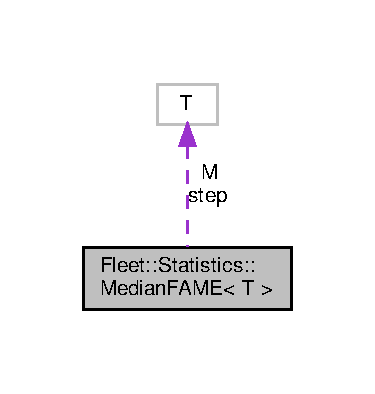
\includegraphics[width=180pt]{class_fleet_1_1_statistics_1_1_median_f_a_m_e__coll__graph}
\end{center}
\end{figure}
\subsection*{Public Member Functions}
\begin{DoxyCompactItemize}
\item 
\hyperlink{class_fleet_1_1_statistics_1_1_median_f_a_m_e_a0be08191b9c7efbadc85e32cf650fe2c}{Median\+F\+A\+ME} ()
\item 
T \hyperlink{class_fleet_1_1_statistics_1_1_median_f_a_m_e_a9ebd0ea21583d80bd9ca2f3cd6f06941}{median} () const
\item 
void \hyperlink{class_fleet_1_1_statistics_1_1_median_f_a_m_e_a676e90f267fc315e67416ec432944896}{add} (T x)
\item 
void \hyperlink{class_fleet_1_1_statistics_1_1_median_f_a_m_e_a5a81f46d3917cd67d5060eb88f7e6cc3}{operator$<$$<$} (T x)
\end{DoxyCompactItemize}
\subsection*{Public Attributes}
\begin{DoxyCompactItemize}
\item 
T \hyperlink{class_fleet_1_1_statistics_1_1_median_f_a_m_e_a5906801f64045cd1dc7555857325c455}{M}
\item 
size\+\_\+t \hyperlink{class_fleet_1_1_statistics_1_1_median_f_a_m_e_abffd20d230e6aa48e8a8d0e33aab157a}{n}
\item 
T \hyperlink{class_fleet_1_1_statistics_1_1_median_f_a_m_e_a3451548541aad22bb7a1c35291faa357}{step}
\end{DoxyCompactItemize}


\subsection{Detailed Description}
\subsubsection*{template$<$typename T$>$\newline
class Fleet\+::\+Statistics\+::\+Median\+F\+A\+M\+E$<$ T $>$}

\begin{DoxyAuthor}{Author}
steven piantadosi 
\end{DoxyAuthor}
\begin{DoxyDate}{Date}
03/02/20 
\end{DoxyDate}


\subsection{Constructor \& Destructor Documentation}
\mbox{\Hypertarget{class_fleet_1_1_statistics_1_1_median_f_a_m_e_a0be08191b9c7efbadc85e32cf650fe2c}\label{class_fleet_1_1_statistics_1_1_median_f_a_m_e_a0be08191b9c7efbadc85e32cf650fe2c}} 
\index{Fleet\+::\+Statistics\+::\+Median\+F\+A\+ME@{Fleet\+::\+Statistics\+::\+Median\+F\+A\+ME}!Median\+F\+A\+ME@{Median\+F\+A\+ME}}
\index{Median\+F\+A\+ME@{Median\+F\+A\+ME}!Fleet\+::\+Statistics\+::\+Median\+F\+A\+ME@{Fleet\+::\+Statistics\+::\+Median\+F\+A\+ME}}
\subsubsection{\texorpdfstring{Median\+F\+A\+M\+E()}{MedianFAME()}}
{\footnotesize\ttfamily template$<$typename T$>$ \\
\hyperlink{class_fleet_1_1_statistics_1_1_median_f_a_m_e}{Fleet\+::\+Statistics\+::\+Median\+F\+A\+ME}$<$ T $>$\+::\hyperlink{class_fleet_1_1_statistics_1_1_median_f_a_m_e}{Median\+F\+A\+ME} (\begin{DoxyParamCaption}{ }\end{DoxyParamCaption})\hspace{0.3cm}{\ttfamily [inline]}}



\subsection{Member Function Documentation}
\mbox{\Hypertarget{class_fleet_1_1_statistics_1_1_median_f_a_m_e_a676e90f267fc315e67416ec432944896}\label{class_fleet_1_1_statistics_1_1_median_f_a_m_e_a676e90f267fc315e67416ec432944896}} 
\index{Fleet\+::\+Statistics\+::\+Median\+F\+A\+ME@{Fleet\+::\+Statistics\+::\+Median\+F\+A\+ME}!add@{add}}
\index{add@{add}!Fleet\+::\+Statistics\+::\+Median\+F\+A\+ME@{Fleet\+::\+Statistics\+::\+Median\+F\+A\+ME}}
\subsubsection{\texorpdfstring{add()}{add()}}
{\footnotesize\ttfamily template$<$typename T$>$ \\
void \hyperlink{class_fleet_1_1_statistics_1_1_median_f_a_m_e}{Fleet\+::\+Statistics\+::\+Median\+F\+A\+ME}$<$ T $>$\+::add (\begin{DoxyParamCaption}\item[{T}]{x }\end{DoxyParamCaption})\hspace{0.3cm}{\ttfamily [inline]}}

\mbox{\Hypertarget{class_fleet_1_1_statistics_1_1_median_f_a_m_e_a9ebd0ea21583d80bd9ca2f3cd6f06941}\label{class_fleet_1_1_statistics_1_1_median_f_a_m_e_a9ebd0ea21583d80bd9ca2f3cd6f06941}} 
\index{Fleet\+::\+Statistics\+::\+Median\+F\+A\+ME@{Fleet\+::\+Statistics\+::\+Median\+F\+A\+ME}!median@{median}}
\index{median@{median}!Fleet\+::\+Statistics\+::\+Median\+F\+A\+ME@{Fleet\+::\+Statistics\+::\+Median\+F\+A\+ME}}
\subsubsection{\texorpdfstring{median()}{median()}}
{\footnotesize\ttfamily template$<$typename T$>$ \\
T \hyperlink{class_fleet_1_1_statistics_1_1_median_f_a_m_e}{Fleet\+::\+Statistics\+::\+Median\+F\+A\+ME}$<$ T $>$\+::median (\begin{DoxyParamCaption}{ }\end{DoxyParamCaption}) const\hspace{0.3cm}{\ttfamily [inline]}}

\mbox{\Hypertarget{class_fleet_1_1_statistics_1_1_median_f_a_m_e_a5a81f46d3917cd67d5060eb88f7e6cc3}\label{class_fleet_1_1_statistics_1_1_median_f_a_m_e_a5a81f46d3917cd67d5060eb88f7e6cc3}} 
\index{Fleet\+::\+Statistics\+::\+Median\+F\+A\+ME@{Fleet\+::\+Statistics\+::\+Median\+F\+A\+ME}!operator$<$$<$@{operator$<$$<$}}
\index{operator$<$$<$@{operator$<$$<$}!Fleet\+::\+Statistics\+::\+Median\+F\+A\+ME@{Fleet\+::\+Statistics\+::\+Median\+F\+A\+ME}}
\subsubsection{\texorpdfstring{operator$<$$<$()}{operator<<()}}
{\footnotesize\ttfamily template$<$typename T$>$ \\
void \hyperlink{class_fleet_1_1_statistics_1_1_median_f_a_m_e}{Fleet\+::\+Statistics\+::\+Median\+F\+A\+ME}$<$ T $>$\+::operator$<$$<$ (\begin{DoxyParamCaption}\item[{T}]{x }\end{DoxyParamCaption})\hspace{0.3cm}{\ttfamily [inline]}}



\subsection{Member Data Documentation}
\mbox{\Hypertarget{class_fleet_1_1_statistics_1_1_median_f_a_m_e_a5906801f64045cd1dc7555857325c455}\label{class_fleet_1_1_statistics_1_1_median_f_a_m_e_a5906801f64045cd1dc7555857325c455}} 
\index{Fleet\+::\+Statistics\+::\+Median\+F\+A\+ME@{Fleet\+::\+Statistics\+::\+Median\+F\+A\+ME}!M@{M}}
\index{M@{M}!Fleet\+::\+Statistics\+::\+Median\+F\+A\+ME@{Fleet\+::\+Statistics\+::\+Median\+F\+A\+ME}}
\subsubsection{\texorpdfstring{M}{M}}
{\footnotesize\ttfamily template$<$typename T$>$ \\
T \hyperlink{class_fleet_1_1_statistics_1_1_median_f_a_m_e}{Fleet\+::\+Statistics\+::\+Median\+F\+A\+ME}$<$ T $>$\+::M}

\mbox{\Hypertarget{class_fleet_1_1_statistics_1_1_median_f_a_m_e_abffd20d230e6aa48e8a8d0e33aab157a}\label{class_fleet_1_1_statistics_1_1_median_f_a_m_e_abffd20d230e6aa48e8a8d0e33aab157a}} 
\index{Fleet\+::\+Statistics\+::\+Median\+F\+A\+ME@{Fleet\+::\+Statistics\+::\+Median\+F\+A\+ME}!n@{n}}
\index{n@{n}!Fleet\+::\+Statistics\+::\+Median\+F\+A\+ME@{Fleet\+::\+Statistics\+::\+Median\+F\+A\+ME}}
\subsubsection{\texorpdfstring{n}{n}}
{\footnotesize\ttfamily template$<$typename T$>$ \\
size\+\_\+t \hyperlink{class_fleet_1_1_statistics_1_1_median_f_a_m_e}{Fleet\+::\+Statistics\+::\+Median\+F\+A\+ME}$<$ T $>$\+::n}

\mbox{\Hypertarget{class_fleet_1_1_statistics_1_1_median_f_a_m_e_a3451548541aad22bb7a1c35291faa357}\label{class_fleet_1_1_statistics_1_1_median_f_a_m_e_a3451548541aad22bb7a1c35291faa357}} 
\index{Fleet\+::\+Statistics\+::\+Median\+F\+A\+ME@{Fleet\+::\+Statistics\+::\+Median\+F\+A\+ME}!step@{step}}
\index{step@{step}!Fleet\+::\+Statistics\+::\+Median\+F\+A\+ME@{Fleet\+::\+Statistics\+::\+Median\+F\+A\+ME}}
\subsubsection{\texorpdfstring{step}{step}}
{\footnotesize\ttfamily template$<$typename T$>$ \\
T \hyperlink{class_fleet_1_1_statistics_1_1_median_f_a_m_e}{Fleet\+::\+Statistics\+::\+Median\+F\+A\+ME}$<$ T $>$\+::step}



The documentation for this class was generated from the following file\+:\begin{DoxyCompactItemize}
\item 
src/\+Statistics/\hyperlink{_median_f_a_m_e_8h}{Median\+F\+A\+M\+E.\+h}\end{DoxyCompactItemize}

\hypertarget{class_my_hypothesis}{}\section{My\+Hypothesis Class Reference}
\label{class_my_hypothesis}\index{My\+Hypothesis@{My\+Hypothesis}}


Inheritance diagram for My\+Hypothesis\+:\nopagebreak
\begin{figure}[H]
\begin{center}
\leavevmode
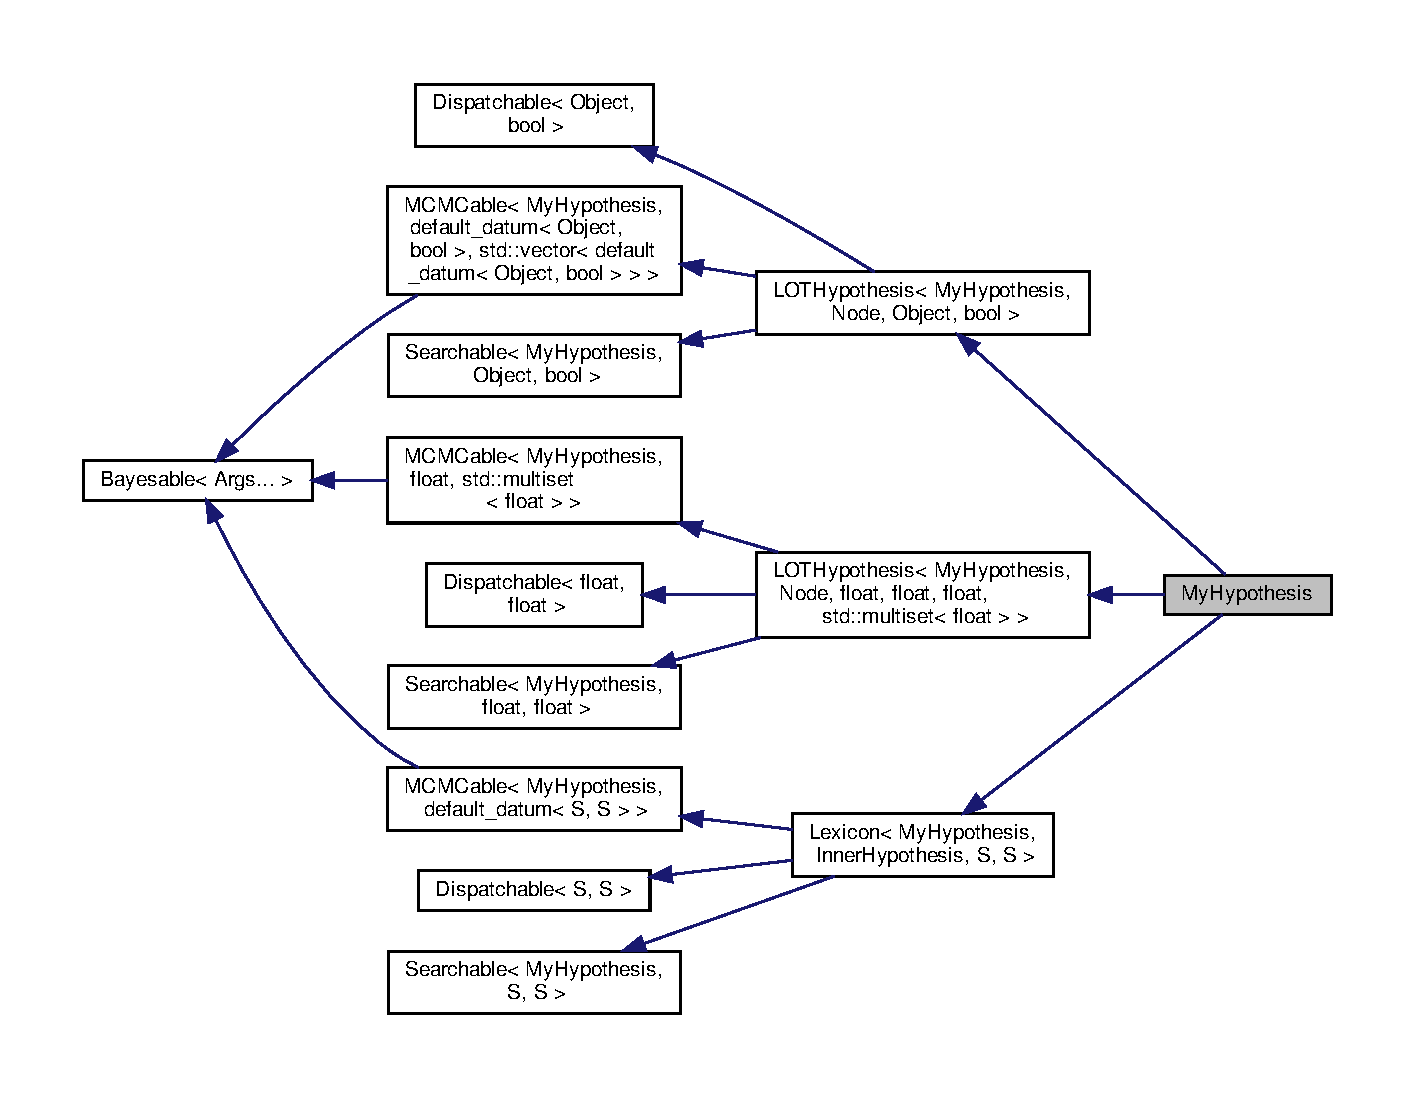
\includegraphics[width=350pt]{class_my_hypothesis__inherit__graph}
\end{center}
\end{figure}


Collaboration diagram for My\+Hypothesis\+:\nopagebreak
\begin{figure}[H]
\begin{center}
\leavevmode
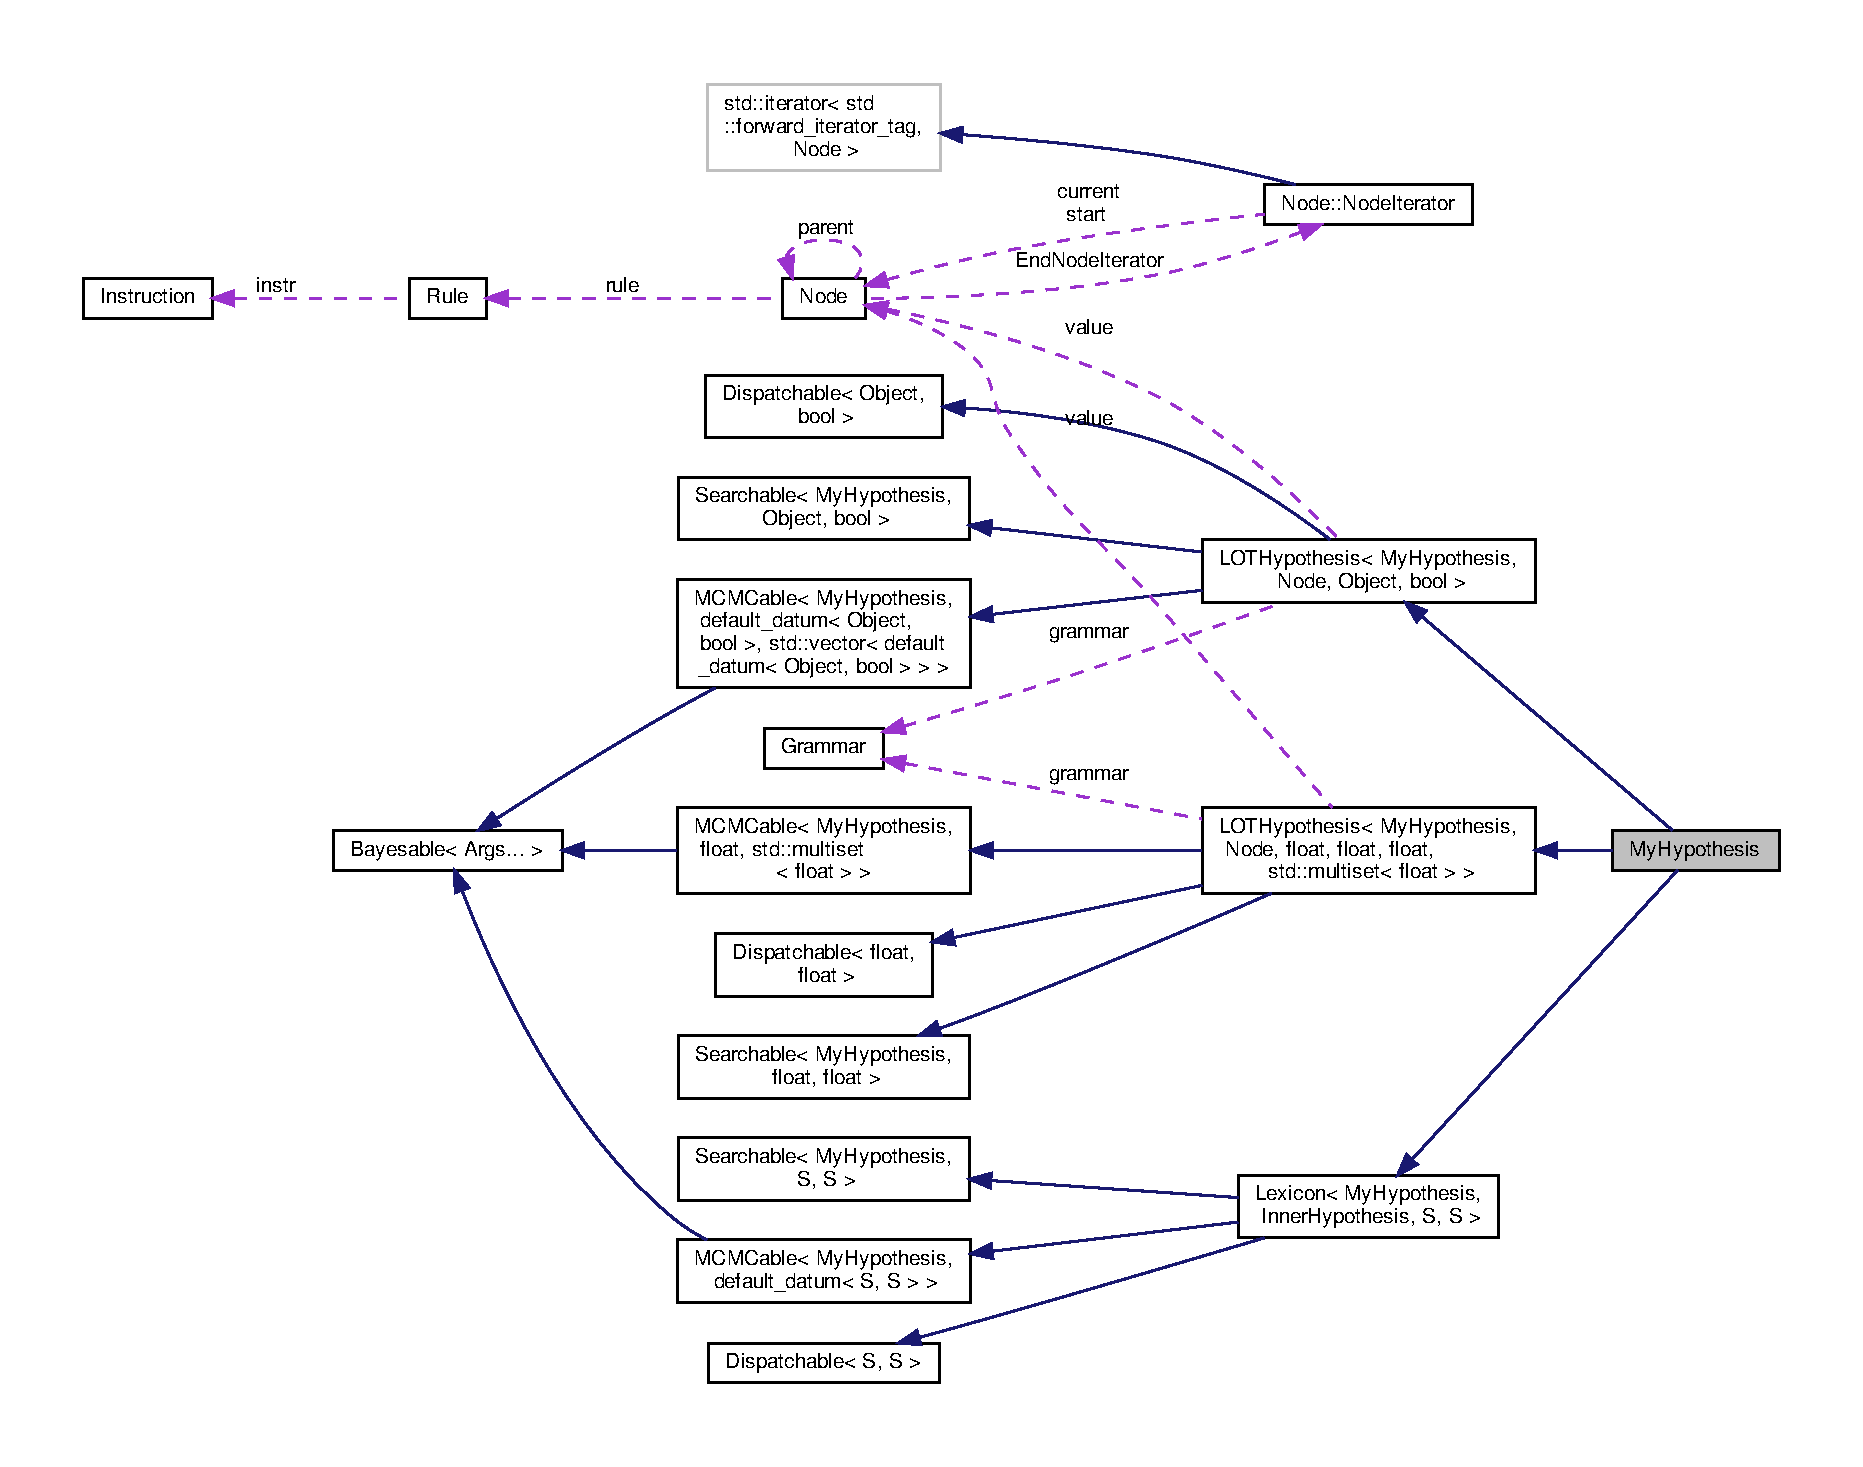
\includegraphics[width=350pt]{class_my_hypothesis__coll__graph}
\end{center}
\end{figure}
\subsection*{Public Types}
\begin{DoxyCompactItemize}
\item 
using \hyperlink{class_my_hypothesis_a266742f266abc638ddc1d1870d735313}{Super} = \hyperlink{class_lexicon}{Lexicon}$<$ \hyperlink{class_my_hypothesis}{My\+Hypothesis}, \hyperlink{class_inner_hypothesis}{Inner\+Hypothesis}, \hyperlink{_formal_language_theory-_complex_2_main_8cpp_a51c40915539205f0b5add30b0d68a4cb}{S}, \hyperlink{_formal_language_theory-_complex_2_main_8cpp_a51c40915539205f0b5add30b0d68a4cb}{S} $>$
\item 
using \hyperlink{class_my_hypothesis_aab716e490381d01aeb22e525eb90e863}{Super} = \hyperlink{class_l_o_t_hypothesis}{L\+O\+T\+Hypothesis}$<$ \hyperlink{class_my_hypothesis}{My\+Hypothesis}, \hyperlink{class_node}{Node}, float, float, float, std\+::multiset$<$ float $>$ $>$
\item 
using \hyperlink{class_my_hypothesis_a8621c1813f3fb8590df10e75be30d4cb}{Super} = \hyperlink{class_l_o_t_hypothesis}{L\+O\+T\+Hypothesis}$<$ \hyperlink{class_my_hypothesis}{My\+Hypothesis}, \hyperlink{class_node}{Node}, \hyperlink{struct_object}{Object}, bool $>$
\end{DoxyCompactItemize}
\subsection*{Public Member Functions}
\begin{DoxyCompactItemize}
\item 
\hyperlink{class_my_hypothesis_ab3ad1dfa93e404fd827df6a57185f5a7}{My\+Hypothesis} ()
\item 
\hyperlink{class_my_hypothesis_a63709659c875c246a506dcff907e1cdd}{My\+Hypothesis} (const \hyperlink{class_my_hypothesis}{My\+Hypothesis} \&h)
\item 
virtual double \hyperlink{class_my_hypothesis_a67752bb4ba61994ef0cb64f7f9031f7f}{compute\+\_\+prior} ()
\begin{DoxyCompactList}\small\item\em Compute the prior -- defaultly not defined. \end{DoxyCompactList}\item 
virtual \hyperlink{class_discrete_distribution}{Discrete\+Distribution}$<$ \hyperlink{_formal_language_theory-_complex_2_main_8cpp_a51c40915539205f0b5add30b0d68a4cb}{S} $>$ \hyperlink{class_my_hypothesis_a016146970c06041b3133f60152a80a24}{call} (const \hyperlink{_formal_language_theory-_complex_2_main_8cpp_a51c40915539205f0b5add30b0d68a4cb}{S} x, const \hyperlink{_formal_language_theory-_complex_2_main_8cpp_a51c40915539205f0b5add30b0d68a4cb}{S} err)
\item 
virtual double \hyperlink{class_my_hypothesis_afcc759336d7f45f01b83807481a10f42}{compute\+\_\+single\+\_\+likelihood} (const \hyperlink{class_bayesable_a7c93a2eeab708378eb321745908718d4}{t\+\_\+datum} \&datum)
\begin{DoxyCompactList}\small\item\em Compute the likelihood of a single data point. \end{DoxyCompactList}\item 
double \hyperlink{class_my_hypothesis_a9caaf0511be161a52f7e93c2086374bc}{compute\+\_\+likelihood} (const \hyperlink{class_bayesable_a70a593a67c7d43239ecc06bb4fd06a6b}{t\+\_\+data} \&data, const double breakout=-\/\hyperlink{_numerics_8h_a1bb1e42ae1b40cad6e99da0aab8a5576}{infinity})
\begin{DoxyCompactList}\small\item\em Compute the likelihood of a collection of data, by calling compute\+\_\+single\+\_\+likelihood on each. This stops if our likelihood falls below breakout. \end{DoxyCompactList}\item 
void \hyperlink{class_my_hypothesis_a682dcd62d83189eae855d6aa4a40b0e0}{print} (std\+::string prefix=\char`\"{}\char`\"{})
\item 
virtual double \hyperlink{class_my_hypothesis_a85348639689176eaf456aaadd63cef2f}{compute\+\_\+likelihood} (const \hyperlink{class_bayesable_a70a593a67c7d43239ecc06bb4fd06a6b}{t\+\_\+data} \&data, const double breakout=-\/\hyperlink{_numerics_8h_a1bb1e42ae1b40cad6e99da0aab8a5576}{infinity})
\begin{DoxyCompactList}\small\item\em Compute the likelihood of a collection of data, by calling compute\+\_\+single\+\_\+likelihood on each. This stops if our likelihood falls below breakout. \end{DoxyCompactList}\item 
\hyperlink{_instruction_8h_a6202215407ab29590bb936ca2996cf64}{vmstatus\+\_\+t} \hyperlink{class_my_hypothesis_a3de47a545e8824bb8c63181965c62a01}{dispatch\+\_\+custom} (\hyperlink{class_instruction}{Instruction} i, \hyperlink{class_virtual_machine_pool}{Virtual\+Machine\+Pool}$<$ float, float $>$ $\ast$pool, \hyperlink{class_virtual_machine_state}{Virtual\+Machine\+State}$<$ float, float $>$ $\ast$vms, \hyperlink{class_dispatchable}{Dispatchable}$<$ float, float $>$ $\ast$loader)
\item 
double \hyperlink{class_my_hypothesis_a5e6bd5e0ebcb987aa4f0adf4295dba11}{compute\+\_\+single\+\_\+likelihood} (const \hyperlink{class_bayesable_a7c93a2eeab708378eb321745908718d4}{t\+\_\+datum} \&x)
\begin{DoxyCompactList}\small\item\em Compute the likelihood of a single data point. \end{DoxyCompactList}\end{DoxyCompactItemize}
\subsection*{Additional Inherited Members}


\subsection{Detailed Description}

\begin{DoxyCode}
    This is a global variable that provides a convenient way to wrap our primitives
    where we can pair up a \textcolor{keyword}{function} with a name, and \hyperlink{_miscellaneous_8h_a9f2587d1070b8924b276ba83988d3667}{pass} that as a constructor
    to the \hyperlink{class_l_o_t_hypothesis_aa7cf638b5d680794e33aa5eb4bd36b09}{grammar}. We need a tuple here because \hyperlink{struct_primitive}{Primitive} has a bunch of \textcolor{keyword}{template}
    types to handle thee \textcolor{keyword}{function} it has, so each is actually a different type.
    This must be defined before we \textcolor{keyword}{import} \hyperlink{namespace_fleet}{Fleet} because \hyperlink{namespace_fleet}{Fleet} does some \textcolor{keyword}{template}
    magic internally
   ~~~~~~~~~~~~~~~~~~~~~~~~~~~~~~~~~~~~~~~~~~~~~~~~~~~~~~~~~~~~~~~~~~~~~~~~~~~~~~~~~~~~~~~~ */




std::tuple PRIMITIVES = \{
    \hyperlink{struct_primitive}{Primitive}(\textcolor{stringliteral}{"and(%s,%s)"},    +[](\textcolor{keywordtype}{bool} a, \textcolor{keywordtype}{bool} b) -> \textcolor{keywordtype}{bool} \{ \textcolor{keywordflow}{return} (a and b); \}, 2.0), \textcolor{comment}{//
       optional specification of prior weight (default=1.0)}
    \hyperlink{struct_primitive}{Primitive}(\textcolor{stringliteral}{"or(%s,%s)"},     +[](\textcolor{keywordtype}{bool} a, \textcolor{keywordtype}{bool} b) -> \textcolor{keywordtype}{bool} \{ \textcolor{keywordflow}{return} (a or b); \}),
    \hyperlink{struct_primitive}{Primitive}(\textcolor{stringliteral}{"not(%s)"},       +[](\textcolor{keywordtype}{bool} a)         -> \textcolor{keywordtype}{bool} \{ \textcolor{keywordflow}{return} (not a); \}),
    \textcolor{comment}{// that + is really insane, but is needed to convert a lambda to a function pointer}

    \hyperlink{struct_primitive}{Primitive}(\textcolor{stringliteral}{"red(%s)"},       +[](\hyperlink{struct_object}{Object} x)       -> \textcolor{keywordtype}{bool} \{ \textcolor{keywordflow}{return} x.
      \hyperlink{struct_object_a3ed85d6e0b0b62ff2501d421cb55c5e9}{color} == \hyperlink{_rational_rules_2_main_8cpp_ab87bacfdad76e61b9412d7124be44c1caee38e4d5dd68c4e440825018d549cb47}{Color::Red}; \}),
    \hyperlink{struct_primitive}{Primitive}(\textcolor{stringliteral}{"green(%s)"},     +[](\hyperlink{struct_object}{Object} x)       -> \textcolor{keywordtype}{bool} \{ \textcolor{keywordflow}{return} x.
      \hyperlink{struct_object_a3ed85d6e0b0b62ff2501d421cb55c5e9}{color} == \hyperlink{_rational_rules_2_main_8cpp_ab87bacfdad76e61b9412d7124be44c1cad382816a3cbeed082c9e216e7392eed1}{Color::Green}; \}),
    \hyperlink{struct_primitive}{Primitive}(\textcolor{stringliteral}{"blue(%s)"},      +[](\hyperlink{struct_object}{Object} x)       -> \textcolor{keywordtype}{bool} \{ \textcolor{keywordflow}{return} x.
      \hyperlink{struct_object_a3ed85d6e0b0b62ff2501d421cb55c5e9}{color} == \hyperlink{_rational_rules_2_main_8cpp_ab87bacfdad76e61b9412d7124be44c1ca9594eec95be70e7b1710f730fdda33d9}{Color::Blue}; \}),

    \hyperlink{struct_primitive}{Primitive}(\textcolor{stringliteral}{"square(%s)"},    +[](\hyperlink{struct_object}{Object} x)       -> \textcolor{keywordtype}{bool} \{ \textcolor{keywordflow}{return} x.
      \hyperlink{struct_object_a09a35e7356709e994637bd66c2c69fc4}{shape} == \hyperlink{_rational_rules_2_main_8cpp_a55b506070847a13554f8b879c1bfb37caceb46ca115d05c51aa5a16a8867c3304}{Shape::Square}; \}),
    \hyperlink{struct_primitive}{Primitive}(\textcolor{stringliteral}{"triangle(%s)"},  +[](\hyperlink{struct_object}{Object} x)       -> \textcolor{keywordtype}{bool} \{ \textcolor{keywordflow}{return} x.
      \hyperlink{struct_object_a09a35e7356709e994637bd66c2c69fc4}{shape} == \hyperlink{_rational_rules_2_main_8cpp_a55b506070847a13554f8b879c1bfb37ca5e5500cb2b82eb72d550de644bd1b64b}{Shape::Triangle}; \}),
    \hyperlink{struct_primitive}{Primitive}(\textcolor{stringliteral}{"circle(%s)"},    +[](\hyperlink{struct_object}{Object} x)       -> \textcolor{keywordtype}{bool} \{ \textcolor{keywordflow}{return} x.
      \hyperlink{struct_object_a09a35e7356709e994637bd66c2c69fc4}{shape} == \hyperlink{_rational_rules_2_main_8cpp_a55b506070847a13554f8b879c1bfb37ca30954d90085f6eaaf5817917fc5fecb3}{Shape::Circle}; \}),


    \textcolor{comment}{// but we also have to add a rule for the BuiltinOp that access x, our argument}
    \hyperlink{struct_builtin_1_1_x}{Builtin::X<Object>}(\textcolor{stringliteral}{"x"}, 10.0)
\};

\textcolor{comment}{// Includes critical files. Also defines some variables (mcts\_steps, explore, etc.) that get processed from
       argv }


\textcolor{comment}{/*}
\end{DoxyCode}
 Define a class for handling my specific hypotheses and data. Everything is defaultly a P\+C\+FG prior and regeneration proposals, but I have to define a likelihood $\sim$$\sim$$\sim$$\sim$$\sim$$\sim$$\sim$$\sim$$\sim$$\sim$$\sim$$\sim$$\sim$$\sim$$\sim$$\sim$$\sim$$\sim$$\sim$$\sim$$\sim$$\sim$$\sim$$\sim$$\sim$$\sim$$\sim$$\sim$$\sim$$\sim$$\sim$$\sim$$\sim$$\sim$$\sim$$\sim$$\sim$$\sim$$\sim$$\sim$$\sim$$\sim$$\sim$$\sim$$\sim$$\sim$$\sim$$\sim$$\sim$$\sim$$\sim$$\sim$$\sim$$\sim$$\sim$$\sim$$\sim$$\sim$$\sim$$\sim$$\sim$$\sim$$\sim$$\sim$$\sim$$\sim$$\sim$$\sim$$\sim$$\sim$$\sim$$\sim$$\sim$$\sim$$\sim$$\sim$$\sim$$\sim$$\sim$$\sim$$\sim$$\sim$$\sim$$\sim$$\sim$$\sim$$\sim$$\sim$ 

\subsection{Member Typedef Documentation}
\mbox{\Hypertarget{class_my_hypothesis_aab716e490381d01aeb22e525eb90e863}\label{class_my_hypothesis_aab716e490381d01aeb22e525eb90e863}} 
\index{My\+Hypothesis@{My\+Hypothesis}!Super@{Super}}
\index{Super@{Super}!My\+Hypothesis@{My\+Hypothesis}}
\subsubsection{\texorpdfstring{Super}{Super}\hspace{0.1cm}{\footnotesize\ttfamily [1/3]}}
{\footnotesize\ttfamily using \hyperlink{class_my_hypothesis_a266742f266abc638ddc1d1870d735313}{My\+Hypothesis\+::\+Super} =  \hyperlink{class_l_o_t_hypothesis}{L\+O\+T\+Hypothesis}$<$\hyperlink{class_my_hypothesis}{My\+Hypothesis},\hyperlink{class_node}{Node},float,float, float, std\+::multiset$<$float$>$ $>$}

\mbox{\Hypertarget{class_my_hypothesis_a8621c1813f3fb8590df10e75be30d4cb}\label{class_my_hypothesis_a8621c1813f3fb8590df10e75be30d4cb}} 
\index{My\+Hypothesis@{My\+Hypothesis}!Super@{Super}}
\index{Super@{Super}!My\+Hypothesis@{My\+Hypothesis}}
\subsubsection{\texorpdfstring{Super}{Super}\hspace{0.1cm}{\footnotesize\ttfamily [2/3]}}
{\footnotesize\ttfamily using \hyperlink{class_my_hypothesis_a266742f266abc638ddc1d1870d735313}{My\+Hypothesis\+::\+Super} =  \hyperlink{class_l_o_t_hypothesis}{L\+O\+T\+Hypothesis}$<$\hyperlink{class_my_hypothesis}{My\+Hypothesis},\hyperlink{class_node}{Node},\hyperlink{struct_object}{Object},bool$>$}

\mbox{\Hypertarget{class_my_hypothesis_a266742f266abc638ddc1d1870d735313}\label{class_my_hypothesis_a266742f266abc638ddc1d1870d735313}} 
\index{My\+Hypothesis@{My\+Hypothesis}!Super@{Super}}
\index{Super@{Super}!My\+Hypothesis@{My\+Hypothesis}}
\subsubsection{\texorpdfstring{Super}{Super}\hspace{0.1cm}{\footnotesize\ttfamily [3/3]}}
{\footnotesize\ttfamily using \hyperlink{class_my_hypothesis_a266742f266abc638ddc1d1870d735313}{My\+Hypothesis\+::\+Super} =  \hyperlink{class_lexicon}{Lexicon}$<$\hyperlink{class_my_hypothesis}{My\+Hypothesis}, \hyperlink{class_inner_hypothesis}{Inner\+Hypothesis}, \hyperlink{_formal_language_theory-_complex_2_main_8cpp_a51c40915539205f0b5add30b0d68a4cb}{S}, \hyperlink{_formal_language_theory-_complex_2_main_8cpp_a51c40915539205f0b5add30b0d68a4cb}{S}$>$}



\subsection{Constructor \& Destructor Documentation}
\mbox{\Hypertarget{class_my_hypothesis_ab3ad1dfa93e404fd827df6a57185f5a7}\label{class_my_hypothesis_ab3ad1dfa93e404fd827df6a57185f5a7}} 
\index{My\+Hypothesis@{My\+Hypothesis}!My\+Hypothesis@{My\+Hypothesis}}
\index{My\+Hypothesis@{My\+Hypothesis}!My\+Hypothesis@{My\+Hypothesis}}
\subsubsection{\texorpdfstring{My\+Hypothesis()}{MyHypothesis()}\hspace{0.1cm}{\footnotesize\ttfamily [1/2]}}
{\footnotesize\ttfamily My\+Hypothesis\+::\+My\+Hypothesis (\begin{DoxyParamCaption}{ }\end{DoxyParamCaption})\hspace{0.3cm}{\ttfamily [inline]}}

\mbox{\Hypertarget{class_my_hypothesis_a63709659c875c246a506dcff907e1cdd}\label{class_my_hypothesis_a63709659c875c246a506dcff907e1cdd}} 
\index{My\+Hypothesis@{My\+Hypothesis}!My\+Hypothesis@{My\+Hypothesis}}
\index{My\+Hypothesis@{My\+Hypothesis}!My\+Hypothesis@{My\+Hypothesis}}
\subsubsection{\texorpdfstring{My\+Hypothesis()}{MyHypothesis()}\hspace{0.1cm}{\footnotesize\ttfamily [2/2]}}
{\footnotesize\ttfamily My\+Hypothesis\+::\+My\+Hypothesis (\begin{DoxyParamCaption}\item[{const \hyperlink{class_my_hypothesis}{My\+Hypothesis} \&}]{h }\end{DoxyParamCaption})\hspace{0.3cm}{\ttfamily [inline]}}



\subsection{Member Function Documentation}
\mbox{\Hypertarget{class_my_hypothesis_a016146970c06041b3133f60152a80a24}\label{class_my_hypothesis_a016146970c06041b3133f60152a80a24}} 
\index{My\+Hypothesis@{My\+Hypothesis}!call@{call}}
\index{call@{call}!My\+Hypothesis@{My\+Hypothesis}}
\subsubsection{\texorpdfstring{call()}{call()}}
{\footnotesize\ttfamily virtual \hyperlink{class_discrete_distribution}{Discrete\+Distribution}$<$\hyperlink{_formal_language_theory-_complex_2_main_8cpp_a51c40915539205f0b5add30b0d68a4cb}{S}$>$ My\+Hypothesis\+::call (\begin{DoxyParamCaption}\item[{const \hyperlink{_formal_language_theory-_complex_2_main_8cpp_a51c40915539205f0b5add30b0d68a4cb}{S}}]{x,  }\item[{const \hyperlink{_formal_language_theory-_complex_2_main_8cpp_a51c40915539205f0b5add30b0d68a4cb}{S}}]{err }\end{DoxyParamCaption})\hspace{0.3cm}{\ttfamily [inline]}, {\ttfamily [virtual]}}



Implements \hyperlink{class_lexicon_aaaff682145f9cb15f7252420fe76f111}{Lexicon$<$ My\+Hypothesis, Inner\+Hypothesis, S, S $>$}.

\mbox{\Hypertarget{class_my_hypothesis_a85348639689176eaf456aaadd63cef2f}\label{class_my_hypothesis_a85348639689176eaf456aaadd63cef2f}} 
\index{My\+Hypothesis@{My\+Hypothesis}!compute\+\_\+likelihood@{compute\+\_\+likelihood}}
\index{compute\+\_\+likelihood@{compute\+\_\+likelihood}!My\+Hypothesis@{My\+Hypothesis}}
\subsubsection{\texorpdfstring{compute\+\_\+likelihood()}{compute\_likelihood()}\hspace{0.1cm}{\footnotesize\ttfamily [1/2]}}
{\footnotesize\ttfamily virtual double My\+Hypothesis\+::compute\+\_\+likelihood (\begin{DoxyParamCaption}\item[{const \hyperlink{class_bayesable_a70a593a67c7d43239ecc06bb4fd06a6b}{t\+\_\+data} \&}]{data,  }\item[{const double}]{breakout = {\ttfamily -\/\hyperlink{_numerics_8h_a1bb1e42ae1b40cad6e99da0aab8a5576}{infinity}} }\end{DoxyParamCaption})\hspace{0.3cm}{\ttfamily [inline]}, {\ttfamily [virtual]}}



Compute the likelihood of a collection of data, by calling compute\+\_\+single\+\_\+likelihood on each. This stops if our likelihood falls below breakout. 


\begin{DoxyParams}{Parameters}
{\em data} & \\
\hline
{\em breakout} & \\
\hline
\end{DoxyParams}
\begin{DoxyReturn}{Returns}

\end{DoxyReturn}


Reimplemented from \hyperlink{class_bayesable_af9547335ae15a5068b10d29aee5056ae}{Bayesable$<$ Args... $>$}.

\mbox{\Hypertarget{class_my_hypothesis_a9caaf0511be161a52f7e93c2086374bc}\label{class_my_hypothesis_a9caaf0511be161a52f7e93c2086374bc}} 
\index{My\+Hypothesis@{My\+Hypothesis}!compute\+\_\+likelihood@{compute\+\_\+likelihood}}
\index{compute\+\_\+likelihood@{compute\+\_\+likelihood}!My\+Hypothesis@{My\+Hypothesis}}
\subsubsection{\texorpdfstring{compute\+\_\+likelihood()}{compute\_likelihood()}\hspace{0.1cm}{\footnotesize\ttfamily [2/2]}}
{\footnotesize\ttfamily double My\+Hypothesis\+::compute\+\_\+likelihood (\begin{DoxyParamCaption}\item[{const \hyperlink{class_bayesable_a70a593a67c7d43239ecc06bb4fd06a6b}{t\+\_\+data} \&}]{data,  }\item[{const double}]{breakout = {\ttfamily -\/\hyperlink{_numerics_8h_a1bb1e42ae1b40cad6e99da0aab8a5576}{infinity}} }\end{DoxyParamCaption})\hspace{0.3cm}{\ttfamily [inline]}, {\ttfamily [virtual]}}



Compute the likelihood of a collection of data, by calling compute\+\_\+single\+\_\+likelihood on each. This stops if our likelihood falls below breakout. 


\begin{DoxyParams}{Parameters}
{\em data} & \\
\hline
{\em breakout} & \\
\hline
\end{DoxyParams}
\begin{DoxyReturn}{Returns}

\end{DoxyReturn}


Reimplemented from \hyperlink{class_bayesable_af9547335ae15a5068b10d29aee5056ae}{Bayesable$<$ Args... $>$}.

\mbox{\Hypertarget{class_my_hypothesis_a67752bb4ba61994ef0cb64f7f9031f7f}\label{class_my_hypothesis_a67752bb4ba61994ef0cb64f7f9031f7f}} 
\index{My\+Hypothesis@{My\+Hypothesis}!compute\+\_\+prior@{compute\+\_\+prior}}
\index{compute\+\_\+prior@{compute\+\_\+prior}!My\+Hypothesis@{My\+Hypothesis}}
\subsubsection{\texorpdfstring{compute\+\_\+prior()}{compute\_prior()}}
{\footnotesize\ttfamily virtual double My\+Hypothesis\+::compute\+\_\+prior (\begin{DoxyParamCaption}{ }\end{DoxyParamCaption})\hspace{0.3cm}{\ttfamily [inline]}, {\ttfamily [virtual]}}



Compute the prior -- defaultly not defined. 



Reimplemented from \hyperlink{class_lexicon_a1ac27e460a361cc90566b92365909324}{Lexicon$<$ My\+Hypothesis, Inner\+Hypothesis, S, S $>$}.

\mbox{\Hypertarget{class_my_hypothesis_a5e6bd5e0ebcb987aa4f0adf4295dba11}\label{class_my_hypothesis_a5e6bd5e0ebcb987aa4f0adf4295dba11}} 
\index{My\+Hypothesis@{My\+Hypothesis}!compute\+\_\+single\+\_\+likelihood@{compute\+\_\+single\+\_\+likelihood}}
\index{compute\+\_\+single\+\_\+likelihood@{compute\+\_\+single\+\_\+likelihood}!My\+Hypothesis@{My\+Hypothesis}}
\subsubsection{\texorpdfstring{compute\+\_\+single\+\_\+likelihood()}{compute\_single\_likelihood()}\hspace{0.1cm}{\footnotesize\ttfamily [1/2]}}
{\footnotesize\ttfamily double My\+Hypothesis\+::compute\+\_\+single\+\_\+likelihood (\begin{DoxyParamCaption}\item[{const \hyperlink{class_bayesable_a7c93a2eeab708378eb321745908718d4}{t\+\_\+datum} \&}]{datum }\end{DoxyParamCaption})\hspace{0.3cm}{\ttfamily [inline]}, {\ttfamily [virtual]}}



Compute the likelihood of a single data point. 


\begin{DoxyParams}{Parameters}
{\em datum} & \\
\hline
\end{DoxyParams}


Reimplemented from \hyperlink{class_l_o_t_hypothesis_aefea6d0e5d94b1fc716dedb9b25b7b26}{L\+O\+T\+Hypothesis$<$ My\+Hypothesis, Node, Object, bool $>$}.

\mbox{\Hypertarget{class_my_hypothesis_afcc759336d7f45f01b83807481a10f42}\label{class_my_hypothesis_afcc759336d7f45f01b83807481a10f42}} 
\index{My\+Hypothesis@{My\+Hypothesis}!compute\+\_\+single\+\_\+likelihood@{compute\+\_\+single\+\_\+likelihood}}
\index{compute\+\_\+single\+\_\+likelihood@{compute\+\_\+single\+\_\+likelihood}!My\+Hypothesis@{My\+Hypothesis}}
\subsubsection{\texorpdfstring{compute\+\_\+single\+\_\+likelihood()}{compute\_single\_likelihood()}\hspace{0.1cm}{\footnotesize\ttfamily [2/2]}}
{\footnotesize\ttfamily virtual double My\+Hypothesis\+::compute\+\_\+single\+\_\+likelihood (\begin{DoxyParamCaption}\item[{const \hyperlink{class_bayesable_a7c93a2eeab708378eb321745908718d4}{t\+\_\+datum} \&}]{datum }\end{DoxyParamCaption})\hspace{0.3cm}{\ttfamily [inline]}, {\ttfamily [virtual]}}



Compute the likelihood of a single data point. 


\begin{DoxyParams}{Parameters}
{\em datum} & \\
\hline
\end{DoxyParams}


Reimplemented from \hyperlink{class_l_o_t_hypothesis_aefea6d0e5d94b1fc716dedb9b25b7b26}{L\+O\+T\+Hypothesis$<$ My\+Hypothesis, Node, Object, bool $>$}.

\mbox{\Hypertarget{class_my_hypothesis_a3de47a545e8824bb8c63181965c62a01}\label{class_my_hypothesis_a3de47a545e8824bb8c63181965c62a01}} 
\index{My\+Hypothesis@{My\+Hypothesis}!dispatch\+\_\+custom@{dispatch\+\_\+custom}}
\index{dispatch\+\_\+custom@{dispatch\+\_\+custom}!My\+Hypothesis@{My\+Hypothesis}}
\subsubsection{\texorpdfstring{dispatch\+\_\+custom()}{dispatch\_custom()}}
{\footnotesize\ttfamily \hyperlink{_instruction_8h_a6202215407ab29590bb936ca2996cf64}{vmstatus\+\_\+t} My\+Hypothesis\+::dispatch\+\_\+custom (\begin{DoxyParamCaption}\item[{\hyperlink{class_instruction}{Instruction}}]{i,  }\item[{\hyperlink{class_virtual_machine_pool}{Virtual\+Machine\+Pool}$<$ float, float $>$ $\ast$}]{pool,  }\item[{\hyperlink{class_virtual_machine_state}{Virtual\+Machine\+State}$<$ float, float $>$ $\ast$}]{vms,  }\item[{\hyperlink{class_dispatchable}{Dispatchable}$<$ float, float $>$ $\ast$}]{loader }\end{DoxyParamCaption})\hspace{0.3cm}{\ttfamily [inline]}, {\ttfamily [virtual]}}



Reimplemented from \hyperlink{class_l_o_t_hypothesis_a6eae1ce4486971909e0245ab9e30ddeb}{L\+O\+T\+Hypothesis$<$ My\+Hypothesis, Node, float, float, float, std\+::multiset$<$ float $>$ $>$}.

\mbox{\Hypertarget{class_my_hypothesis_a682dcd62d83189eae855d6aa4a40b0e0}\label{class_my_hypothesis_a682dcd62d83189eae855d6aa4a40b0e0}} 
\index{My\+Hypothesis@{My\+Hypothesis}!print@{print}}
\index{print@{print}!My\+Hypothesis@{My\+Hypothesis}}
\subsubsection{\texorpdfstring{print()}{print()}}
{\footnotesize\ttfamily void My\+Hypothesis\+::print (\begin{DoxyParamCaption}\item[{std\+::string}]{prefix = {\ttfamily \char`\"{}\char`\"{}} }\end{DoxyParamCaption})\hspace{0.3cm}{\ttfamily [inline]}, {\ttfamily [virtual]}}



Reimplemented from \hyperlink{class_bayesable_a3f31fa34270083429fb23da21ad50432}{Bayesable$<$ Args... $>$}.



The documentation for this class was generated from the following file\+:\begin{DoxyCompactItemize}
\item 
Models/\+Formal\+Language\+Theory-\/\+Complex/\hyperlink{_formal_language_theory-_complex_2_main_8cpp}{Main.\+cpp}\end{DoxyCompactItemize}

\hypertarget{class_node}{}\section{Node Class Reference}
\label{class_node}\index{Node@{Node}}


{\ttfamily \#include $<$Node.\+h$>$}



Collaboration diagram for Node\+:\nopagebreak
\begin{figure}[H]
\begin{center}
\leavevmode
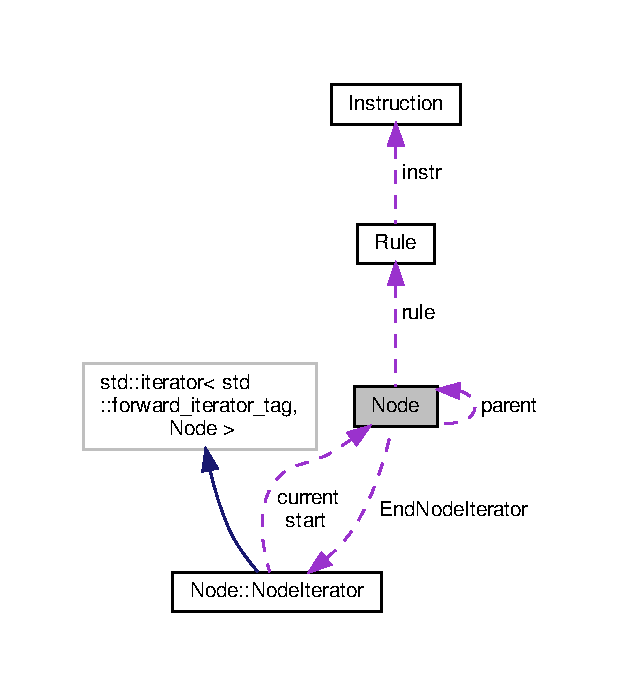
\includegraphics[width=299pt]{class_node__coll__graph}
\end{center}
\end{figure}
\subsection*{Classes}
\begin{DoxyCompactItemize}
\item 
class \hyperlink{class_node_1_1_node_iterator}{Node\+Iterator}
\end{DoxyCompactItemize}
\subsection*{Public Member Functions}
\begin{DoxyCompactItemize}
\item 
\hyperlink{class_node_ae33050869651f64551da2d13ad2a9dbc}{Node} (const \hyperlink{class_rule}{Rule} $\ast$r=nullptr, double \+\_\+lp=0.\+0, bool cr=true)
\item 
\hyperlink{class_node_a277918b68827f6ffd8150f450b0c12c3}{Node} (const \hyperlink{class_node}{Node} \&n)
\item 
\hyperlink{class_node_a87c9938dcd77c169802a732c98204945}{Node} (\hyperlink{class_node}{Node} \&\&n)
\item 
\hyperlink{class_node}{Node} \& \hyperlink{class_node_a23adfa03c20f4141b1105c5b4b1bca3f}{child} (const size\+\_\+t i)
\item 
const \hyperlink{class_node}{Node} \& \hyperlink{class_node_acc2b20cdba470853f1c137e26546ed3c}{child} (const size\+\_\+t i) const
\item 
\hyperlink{_nonterminal_8h_a5c1f658dc7560600a16d22408bd716ca}{nonterminal\+\_\+t} \hyperlink{class_node_aa727c354e38f60fb1560d72ae1aaa9af}{type} (const size\+\_\+t i) const
\item 
size\+\_\+t \hyperlink{class_node_a5d42219573573f6a91cdfe68fe415505}{nchildren} () const
\item 
void \hyperlink{class_node_a1c03973664fcfdfb191feb67f565168b}{fill} ()
\item 
void \hyperlink{class_node_addbfe90949f473c91203389f48095cf0}{operator=} (const \hyperlink{class_node}{Node} \&n)
\item 
void \hyperlink{class_node_abcd5c8ca2ea54716a72f7e27f9a9c937}{operator=} (\hyperlink{class_node}{Node} \&\&n)
\item 
bool \hyperlink{class_node_a8b05feb361beb04d465619751a2297b1}{operator$<$} (const \hyperlink{class_node}{Node} \&n) const
\item 
\hyperlink{class_node_1_1_node_iterator}{Node\+Iterator} \hyperlink{class_node_a319b65eca94c9438201ebda99ab90a65}{begin} () const
\item 
\hyperlink{class_node_1_1_node_iterator}{Node\+Iterator} \hyperlink{class_node_aea7c6e778d4720fb8071af71c57b1628}{end} () const
\item 
\hyperlink{class_node}{Node} $\ast$ \hyperlink{class_node_ac6d1a1d71a28168b34e9092568570738}{left\+\_\+descend} () const
\item 
void \hyperlink{class_node_a8f25f44608c0b19fe02eaf19ade9ea68}{fix\+\_\+child\+\_\+info} ()
\item 
\hyperlink{_nonterminal_8h_a5c1f658dc7560600a16d22408bd716ca}{nonterminal\+\_\+t} \hyperlink{class_node_a4abe3acdc804489a01ef13a25b130fd8}{nt} () const
\item 
\hyperlink{class_node}{Node} \& \hyperlink{class_node_a0b89084e2c7416379edb7c537edcc8f2}{operator\mbox{[}$\,$\mbox{]}} (const size\+\_\+t i)
\item 
const \hyperlink{class_node}{Node} \& \hyperlink{class_node_a8bdfdaa5eb291ae5fb417f45fb8a3633}{operator\mbox{[}$\,$\mbox{]}} (const size\+\_\+t i) const
\item 
void \hyperlink{class_node_afff50c3712b8e30fffd479cad4eee023}{set\+\_\+child} (size\+\_\+t i, \hyperlink{class_node}{Node} \&n)
\item 
void \hyperlink{class_node_a486882370d2c9592c6eabb52a3289253}{set\+\_\+child} (size\+\_\+t i, \hyperlink{class_node}{Node} \&\&n)
\item 
void \hyperlink{class_node_a1a6f6c8062e66046c302a80cc7e8d817}{set\+\_\+to} (\hyperlink{class_node}{Node} \&n)
\item 
void \hyperlink{class_node_a10c63ea2ec819dc5b195c4df33cde113}{set\+\_\+to} (\hyperlink{class_node}{Node} \&\&n)
\item 
bool \hyperlink{class_node_a895ef3b66f975fbaec1e5866a57afbed}{is\+\_\+null} () const
\item 
{\footnotesize template$<$typename T $>$ }\\T \hyperlink{class_node_ac91282056a0df2835f1579bdd21c93e1}{sum} (std\+::function$<$ T(const \hyperlink{class_node}{Node} \&)$>$ \&f) const
\item 
{\footnotesize template$<$typename T $>$ }\\T \hyperlink{class_node_a089e99addd93f91b2ef5a9d0c3e6bdeb}{sum} (T($\ast$f)(const \hyperlink{class_node}{Node} \&)) const
\item 
void \hyperlink{class_node_adefac3cb7b411321c5af15dad1484834}{map} (const std\+::function$<$ void(\hyperlink{class_node}{Node} \&)$>$ \&f)
\item 
void \hyperlink{class_node_a4337bb93da78e142c6171fd81acab93c}{map\+\_\+const} (const std\+::function$<$ void(const \hyperlink{class_node}{Node} \&)$>$ \&f) const
\item 
void \hyperlink{class_node_a59da25cea338385d73b898b86492f97e}{rmap\+\_\+const} (const std\+::function$<$ void(const \hyperlink{class_node}{Node} \&)$>$ \&f) const
\item 
virtual size\+\_\+t \hyperlink{class_node_abd387b27e1deb45b789ad7b7abd8c6e6}{count} () const
\item 
virtual size\+\_\+t \hyperlink{class_node_a0cc58478d98361566830a8d3db745718}{count} (const \hyperlink{class_node}{Node} \&n) const
\item 
virtual bool \hyperlink{class_node_ad12a96da2fe796616aa22e20429f41d5}{is\+\_\+root} () const
\item 
virtual bool \hyperlink{class_node_ac3c263a4e0c734c34aaf62f80f84cd9a}{is\+\_\+terminal} () const
\item 
virtual size\+\_\+t \hyperlink{class_node_a70c820eaeaa852e3c0a46cf006026c1b}{count\+\_\+terminals} () const
\item 
virtual bool \hyperlink{class_node_ac2e36754ba8b1b1d452deeb2bdbd346f}{is\+\_\+complete} () const
\item 
virtual \hyperlink{class_node}{Node} $\ast$ \hyperlink{class_node_a93fc84b584f080593978d3a39631d3e5}{get\+\_\+nth} (int n, std\+::function$<$ int(const \hyperlink{class_node}{Node} \&)$>$ \&f)
\item 
virtual \hyperlink{class_node}{Node} $\ast$ \hyperlink{class_node_a224c0ee6dae35ddce70f8fd3b91e0b1c}{get\+\_\+nth} (int n)
\item 
virtual std\+::string \hyperlink{class_node_a0590ae269543416be9c4ebdf70bad73b}{string} () const
\item 
virtual std\+::string \hyperlink{class_node_a70e879ceb71f47787137572d9bee8efa}{parseable} () const
\item 
virtual size\+\_\+t \hyperlink{class_node_a377548bcf1be99ac5181f9434c33c81e}{program\+\_\+size} () const
\item 
virtual void \hyperlink{class_node_ac995508e96e112675fde53e7748e41bc}{linearize} (Program \&ops) const
\item 
virtual bool \hyperlink{class_node_a90aeee00ccda27f36bea9cdd774eae8d}{operator==} (const \hyperlink{class_node}{Node} \&n) const
\item 
virtual size\+\_\+t \hyperlink{class_node_a212f2e1ba4ff71de6954b0b791d89979}{hash} (size\+\_\+t depth=0) const
\end{DoxyCompactItemize}
\subsection*{Public Attributes}
\begin{DoxyCompactItemize}
\item 
\hyperlink{class_node}{Node} $\ast$ \hyperlink{class_node_ad8184598cdea70e4bbdfd76f2b0f9e85}{parent}
\item 
size\+\_\+t \hyperlink{class_node_ad8e140a5af4e5c312141f2b7af255520}{pi}
\item 
const \hyperlink{class_rule}{Rule} $\ast$ \hyperlink{class_node_a02f5c9463cceb270ad5730760f19c722}{rule}
\item 
double \hyperlink{class_node_a298eaa3743b774a3f9ef396e1dc42a08}{lp}
\item 
bool \hyperlink{class_node_a98c14a51b240fbc7e438f40a12276257}{can\+\_\+resample}
\end{DoxyCompactItemize}
\subsection*{Static Public Attributes}
\begin{DoxyCompactItemize}
\item 
static const char \hyperlink{class_node_abd26102ffbe2a3e00c34bed5508b3234}{N\+T\+Delimiter} = \textquotesingle{}\+:\textquotesingle{}
\item 
static const char \hyperlink{class_node_ab58932e82964fb75ba806870c4069dc2}{Rule\+Delimiter} = \textquotesingle{};\textquotesingle{}
\item 
static \hyperlink{class_node_1_1_node_iterator}{Node\+Iterator} \hyperlink{class_node_a336943f2e37a2b6fcbe8b47634719dec}{End\+Node\+Iterator} = \hyperlink{class_node_1_1_node_iterator}{Node\+Iterator}(nullptr)
\end{DoxyCompactItemize}
\subsection*{Protected Attributes}
\begin{DoxyCompactItemize}
\item 
std\+::vector$<$ \hyperlink{class_node}{Node} $>$ \hyperlink{class_node_af7ddc81358470c3bf7a7819c8b77f53d}{children}
\end{DoxyCompactItemize}


\subsection{Constructor \& Destructor Documentation}
\mbox{\Hypertarget{class_node_ae33050869651f64551da2d13ad2a9dbc}\label{class_node_ae33050869651f64551da2d13ad2a9dbc}} 
\index{Node@{Node}!Node@{Node}}
\index{Node@{Node}!Node@{Node}}
\subsubsection{\texorpdfstring{Node()}{Node()}\hspace{0.1cm}{\footnotesize\ttfamily [1/3]}}
{\footnotesize\ttfamily Node\+::\+Node (\begin{DoxyParamCaption}\item[{const \hyperlink{class_rule}{Rule} $\ast$}]{r = {\ttfamily nullptr},  }\item[{double}]{\+\_\+lp = {\ttfamily 0.0},  }\item[{bool}]{cr = {\ttfamily true} }\end{DoxyParamCaption})\hspace{0.3cm}{\ttfamily [inline]}}

\mbox{\Hypertarget{class_node_a277918b68827f6ffd8150f450b0c12c3}\label{class_node_a277918b68827f6ffd8150f450b0c12c3}} 
\index{Node@{Node}!Node@{Node}}
\index{Node@{Node}!Node@{Node}}
\subsubsection{\texorpdfstring{Node()}{Node()}\hspace{0.1cm}{\footnotesize\ttfamily [2/3]}}
{\footnotesize\ttfamily Node\+::\+Node (\begin{DoxyParamCaption}\item[{const \hyperlink{class_node}{Node} \&}]{n }\end{DoxyParamCaption})\hspace{0.3cm}{\ttfamily [inline]}}

\mbox{\Hypertarget{class_node_a87c9938dcd77c169802a732c98204945}\label{class_node_a87c9938dcd77c169802a732c98204945}} 
\index{Node@{Node}!Node@{Node}}
\index{Node@{Node}!Node@{Node}}
\subsubsection{\texorpdfstring{Node()}{Node()}\hspace{0.1cm}{\footnotesize\ttfamily [3/3]}}
{\footnotesize\ttfamily Node\+::\+Node (\begin{DoxyParamCaption}\item[{\hyperlink{class_node}{Node} \&\&}]{n }\end{DoxyParamCaption})\hspace{0.3cm}{\ttfamily [inline]}}



\subsection{Member Function Documentation}
\mbox{\Hypertarget{class_node_a319b65eca94c9438201ebda99ab90a65}\label{class_node_a319b65eca94c9438201ebda99ab90a65}} 
\index{Node@{Node}!begin@{begin}}
\index{begin@{begin}!Node@{Node}}
\subsubsection{\texorpdfstring{begin()}{begin()}}
{\footnotesize\ttfamily \hyperlink{class_node_1_1_node_iterator}{Node\+Iterator} Node\+::begin (\begin{DoxyParamCaption}{ }\end{DoxyParamCaption}) const\hspace{0.3cm}{\ttfamily [inline]}}

\mbox{\Hypertarget{class_node_a23adfa03c20f4141b1105c5b4b1bca3f}\label{class_node_a23adfa03c20f4141b1105c5b4b1bca3f}} 
\index{Node@{Node}!child@{child}}
\index{child@{child}!Node@{Node}}
\subsubsection{\texorpdfstring{child()}{child()}\hspace{0.1cm}{\footnotesize\ttfamily [1/2]}}
{\footnotesize\ttfamily \hyperlink{class_node}{Node}\& Node\+::child (\begin{DoxyParamCaption}\item[{const size\+\_\+t}]{i }\end{DoxyParamCaption})\hspace{0.3cm}{\ttfamily [inline]}}

Get a reference to my i\textquotesingle{}th child 
\begin{DoxyParams}{Parameters}
{\em i} & \\
\hline
\end{DoxyParams}
\begin{DoxyReturn}{Returns}

\end{DoxyReturn}
\mbox{\Hypertarget{class_node_acc2b20cdba470853f1c137e26546ed3c}\label{class_node_acc2b20cdba470853f1c137e26546ed3c}} 
\index{Node@{Node}!child@{child}}
\index{child@{child}!Node@{Node}}
\subsubsection{\texorpdfstring{child()}{child()}\hspace{0.1cm}{\footnotesize\ttfamily [2/2]}}
{\footnotesize\ttfamily const \hyperlink{class_node}{Node}\& Node\+::child (\begin{DoxyParamCaption}\item[{const size\+\_\+t}]{i }\end{DoxyParamCaption}) const\hspace{0.3cm}{\ttfamily [inline]}}

Constant reference to the i\textquotesingle{}th child 
\begin{DoxyParams}{Parameters}
{\em i} & \\
\hline
\end{DoxyParams}
\begin{DoxyReturn}{Returns}

\end{DoxyReturn}
\mbox{\Hypertarget{class_node_abd387b27e1deb45b789ad7b7abd8c6e6}\label{class_node_abd387b27e1deb45b789ad7b7abd8c6e6}} 
\index{Node@{Node}!count@{count}}
\index{count@{count}!Node@{Node}}
\subsubsection{\texorpdfstring{count()}{count()}\hspace{0.1cm}{\footnotesize\ttfamily [1/2]}}
{\footnotesize\ttfamily virtual size\+\_\+t Node\+::count (\begin{DoxyParamCaption}{ }\end{DoxyParamCaption}) const\hspace{0.3cm}{\ttfamily [inline]}, {\ttfamily [virtual]}}

How many nodes are below me? \begin{DoxyReturn}{Returns}

\end{DoxyReturn}
\mbox{\Hypertarget{class_node_a0cc58478d98361566830a8d3db745718}\label{class_node_a0cc58478d98361566830a8d3db745718}} 
\index{Node@{Node}!count@{count}}
\index{count@{count}!Node@{Node}}
\subsubsection{\texorpdfstring{count()}{count()}\hspace{0.1cm}{\footnotesize\ttfamily [2/2]}}
{\footnotesize\ttfamily virtual size\+\_\+t Node\+::count (\begin{DoxyParamCaption}\item[{const \hyperlink{class_node}{Node} \&}]{n }\end{DoxyParamCaption}) const\hspace{0.3cm}{\ttfamily [inline]}, {\ttfamily [virtual]}}

How many nodes below me are equal to n? 
\begin{DoxyParams}{Parameters}
{\em n} & \\
\hline
\end{DoxyParams}
\begin{DoxyReturn}{Returns}

\end{DoxyReturn}
\mbox{\Hypertarget{class_node_a70c820eaeaa852e3c0a46cf006026c1b}\label{class_node_a70c820eaeaa852e3c0a46cf006026c1b}} 
\index{Node@{Node}!count\+\_\+terminals@{count\+\_\+terminals}}
\index{count\+\_\+terminals@{count\+\_\+terminals}!Node@{Node}}
\subsubsection{\texorpdfstring{count\+\_\+terminals()}{count\_terminals()}}
{\footnotesize\ttfamily virtual size\+\_\+t Node\+::count\+\_\+terminals (\begin{DoxyParamCaption}{ }\end{DoxyParamCaption}) const\hspace{0.3cm}{\ttfamily [inline]}, {\ttfamily [virtual]}}

How many terminals are below me? \begin{DoxyReturn}{Returns}

\end{DoxyReturn}
\mbox{\Hypertarget{class_node_aea7c6e778d4720fb8071af71c57b1628}\label{class_node_aea7c6e778d4720fb8071af71c57b1628}} 
\index{Node@{Node}!end@{end}}
\index{end@{end}!Node@{Node}}
\subsubsection{\texorpdfstring{end()}{end()}}
{\footnotesize\ttfamily \hyperlink{class_node_1_1_node_iterator}{Node\+Iterator} Node\+::end (\begin{DoxyParamCaption}{ }\end{DoxyParamCaption}) const\hspace{0.3cm}{\ttfamily [inline]}}

\mbox{\Hypertarget{class_node_a1c03973664fcfdfb191feb67f565168b}\label{class_node_a1c03973664fcfdfb191feb67f565168b}} 
\index{Node@{Node}!fill@{fill}}
\index{fill@{fill}!Node@{Node}}
\subsubsection{\texorpdfstring{fill()}{fill()}}
{\footnotesize\ttfamily void Node\+::fill (\begin{DoxyParamCaption}{ }\end{DoxyParamCaption})\hspace{0.3cm}{\ttfamily [inline]}}

Fill in all of my immediate children with Null nodes (via Null\+Rule)\mbox{\Hypertarget{class_node_a8f25f44608c0b19fe02eaf19ade9ea68}\label{class_node_a8f25f44608c0b19fe02eaf19ade9ea68}} 
\index{Node@{Node}!fix\+\_\+child\+\_\+info@{fix\+\_\+child\+\_\+info}}
\index{fix\+\_\+child\+\_\+info@{fix\+\_\+child\+\_\+info}!Node@{Node}}
\subsubsection{\texorpdfstring{fix\+\_\+child\+\_\+info()}{fix\_child\_info()}}
{\footnotesize\ttfamily void Node\+::fix\+\_\+child\+\_\+info (\begin{DoxyParamCaption}{ }\end{DoxyParamCaption})\hspace{0.3cm}{\ttfamily [inline]}}

Fix my immediate children\textquotesingle{}s pointers to ensure that children\textquotesingle{}s parent pointers and indices are correct.\mbox{\Hypertarget{class_node_a93fc84b584f080593978d3a39631d3e5}\label{class_node_a93fc84b584f080593978d3a39631d3e5}} 
\index{Node@{Node}!get\+\_\+nth@{get\+\_\+nth}}
\index{get\+\_\+nth@{get\+\_\+nth}!Node@{Node}}
\subsubsection{\texorpdfstring{get\+\_\+nth()}{get\_nth()}\hspace{0.1cm}{\footnotesize\ttfamily [1/2]}}
{\footnotesize\ttfamily virtual \hyperlink{class_node}{Node}$\ast$ Node\+::get\+\_\+nth (\begin{DoxyParamCaption}\item[{int}]{n,  }\item[{std\+::function$<$ int(const \hyperlink{class_node}{Node} \&)$>$ \&}]{f }\end{DoxyParamCaption})\hspace{0.3cm}{\ttfamily [inline]}, {\ttfamily [virtual]}}

Return a pointer to the n\textquotesingle{}th child satisfying f (f\textquotesingle{}s output is cast to bool) 
\begin{DoxyParams}{Parameters}
{\em n} & \\
\hline
{\em f} & \\
\hline
\end{DoxyParams}
\begin{DoxyReturn}{Returns}

\end{DoxyReturn}
\mbox{\Hypertarget{class_node_a224c0ee6dae35ddce70f8fd3b91e0b1c}\label{class_node_a224c0ee6dae35ddce70f8fd3b91e0b1c}} 
\index{Node@{Node}!get\+\_\+nth@{get\+\_\+nth}}
\index{get\+\_\+nth@{get\+\_\+nth}!Node@{Node}}
\subsubsection{\texorpdfstring{get\+\_\+nth()}{get\_nth()}\hspace{0.1cm}{\footnotesize\ttfamily [2/2]}}
{\footnotesize\ttfamily virtual \hyperlink{class_node}{Node}$\ast$ Node\+::get\+\_\+nth (\begin{DoxyParamCaption}\item[{int}]{n }\end{DoxyParamCaption})\hspace{0.3cm}{\ttfamily [inline]}, {\ttfamily [virtual]}}

\mbox{\Hypertarget{class_node_a212f2e1ba4ff71de6954b0b791d89979}\label{class_node_a212f2e1ba4ff71de6954b0b791d89979}} 
\index{Node@{Node}!hash@{hash}}
\index{hash@{hash}!Node@{Node}}
\subsubsection{\texorpdfstring{hash()}{hash()}}
{\footnotesize\ttfamily virtual size\+\_\+t Node\+::hash (\begin{DoxyParamCaption}\item[{size\+\_\+t}]{depth = {\ttfamily 0} }\end{DoxyParamCaption}) const\hspace{0.3cm}{\ttfamily [inline]}, {\ttfamily [virtual]}}

Hash a tree by hashing the rule and everything below. 
\begin{DoxyParams}{Parameters}
{\em depth} & \\
\hline
\end{DoxyParams}
\begin{DoxyReturn}{Returns}

\end{DoxyReturn}
\mbox{\Hypertarget{class_node_ac2e36754ba8b1b1d452deeb2bdbd346f}\label{class_node_ac2e36754ba8b1b1d452deeb2bdbd346f}} 
\index{Node@{Node}!is\+\_\+complete@{is\+\_\+complete}}
\index{is\+\_\+complete@{is\+\_\+complete}!Node@{Node}}
\subsubsection{\texorpdfstring{is\+\_\+complete()}{is\_complete()}}
{\footnotesize\ttfamily virtual bool Node\+::is\+\_\+complete (\begin{DoxyParamCaption}{ }\end{DoxyParamCaption}) const\hspace{0.3cm}{\ttfamily [inline]}, {\ttfamily [virtual]}}

A tree is complete if it contains no null nodes below it. \begin{DoxyReturn}{Returns}

\end{DoxyReturn}
\mbox{\Hypertarget{class_node_a895ef3b66f975fbaec1e5866a57afbed}\label{class_node_a895ef3b66f975fbaec1e5866a57afbed}} 
\index{Node@{Node}!is\+\_\+null@{is\+\_\+null}}
\index{is\+\_\+null@{is\+\_\+null}!Node@{Node}}
\subsubsection{\texorpdfstring{is\+\_\+null()}{is\_null()}}
{\footnotesize\ttfamily bool Node\+::is\+\_\+null (\begin{DoxyParamCaption}{ }\end{DoxyParamCaption}) const\hspace{0.3cm}{\ttfamily [inline]}}

Am I a null node? \begin{DoxyReturn}{Returns}

\end{DoxyReturn}
\mbox{\Hypertarget{class_node_ad12a96da2fe796616aa22e20429f41d5}\label{class_node_ad12a96da2fe796616aa22e20429f41d5}} 
\index{Node@{Node}!is\+\_\+root@{is\+\_\+root}}
\index{is\+\_\+root@{is\+\_\+root}!Node@{Node}}
\subsubsection{\texorpdfstring{is\+\_\+root()}{is\_root()}}
{\footnotesize\ttfamily virtual bool Node\+::is\+\_\+root (\begin{DoxyParamCaption}{ }\end{DoxyParamCaption}) const\hspace{0.3cm}{\ttfamily [inline]}, {\ttfamily [virtual]}}

Am I a root node? I am if my parent is nullptr. \begin{DoxyReturn}{Returns}

\end{DoxyReturn}
\mbox{\Hypertarget{class_node_ac3c263a4e0c734c34aaf62f80f84cd9a}\label{class_node_ac3c263a4e0c734c34aaf62f80f84cd9a}} 
\index{Node@{Node}!is\+\_\+terminal@{is\+\_\+terminal}}
\index{is\+\_\+terminal@{is\+\_\+terminal}!Node@{Node}}
\subsubsection{\texorpdfstring{is\+\_\+terminal()}{is\_terminal()}}
{\footnotesize\ttfamily virtual bool Node\+::is\+\_\+terminal (\begin{DoxyParamCaption}{ }\end{DoxyParamCaption}) const\hspace{0.3cm}{\ttfamily [inline]}, {\ttfamily [virtual]}}

Am I a terminal? I am if I have no children. \begin{DoxyReturn}{Returns}

\end{DoxyReturn}
\mbox{\Hypertarget{class_node_ac6d1a1d71a28168b34e9092568570738}\label{class_node_ac6d1a1d71a28168b34e9092568570738}} 
\index{Node@{Node}!left\+\_\+descend@{left\+\_\+descend}}
\index{left\+\_\+descend@{left\+\_\+descend}!Node@{Node}}
\subsubsection{\texorpdfstring{left\+\_\+descend()}{left\_descend()}}
{\footnotesize\ttfamily \hyperlink{class_node}{Node}$\ast$ Node\+::left\+\_\+descend (\begin{DoxyParamCaption}{ }\end{DoxyParamCaption}) const\hspace{0.3cm}{\ttfamily [inline]}}

Go down a tree and find the leftmost child \begin{DoxyReturn}{Returns}

\end{DoxyReturn}
\mbox{\Hypertarget{class_node_ac995508e96e112675fde53e7748e41bc}\label{class_node_ac995508e96e112675fde53e7748e41bc}} 
\index{Node@{Node}!linearize@{linearize}}
\index{linearize@{linearize}!Node@{Node}}
\subsubsection{\texorpdfstring{linearize()}{linearize()}}
{\footnotesize\ttfamily virtual void Node\+::linearize (\begin{DoxyParamCaption}\item[{Program \&}]{ops }\end{DoxyParamCaption}) const\hspace{0.3cm}{\ttfamily [inline]}, {\ttfamily [virtual]}}

convert tree to a linear sequence of operations. To do this, we first linearize the kids, leaving their values as the top on the stack then we compute our value, remove our kids\textquotesingle{} values to clean up the stack, and push on our return the only fanciness is for if\+: here we will use the following layout $<$\+T\+O\+P of=\char`\"{}\char`\"{} stack$>$=\char`\"{}\char`\"{}$>$ $<$bool$>$ \hyperlink{_instruction_8h_af2fb7c87c5854c5733d7bb0506b06de7a8f69a9fe993189d72cf7b07e8517801d}{op\+\_\+\+I\+F(xsize)} X-\/branch J\+U\+M\+P(ysize) Y-\/branch

N\+O\+TE\+: Inline here lets gcc inline a few recursions of this function, which ends up speeding us up a bit (otherwise recursive inlining only happens at -\/\+O3) This optimization is why we do set max-\/inline-\/insns-\/recursive in Fleet.\+mk 
\begin{DoxyParams}{Parameters}
{\em ops} & \\
\hline
\end{DoxyParams}
\mbox{\Hypertarget{class_node_adefac3cb7b411321c5af15dad1484834}\label{class_node_adefac3cb7b411321c5af15dad1484834}} 
\index{Node@{Node}!map@{map}}
\index{map@{map}!Node@{Node}}
\subsubsection{\texorpdfstring{map()}{map()}}
{\footnotesize\ttfamily void Node\+::map (\begin{DoxyParamCaption}\item[{const std\+::function$<$ void(\hyperlink{class_node}{Node} \&)$>$ \&}]{f }\end{DoxyParamCaption})\hspace{0.3cm}{\ttfamily [inline]}}

Apply f to me and everything below. 
\begin{DoxyParams}{Parameters}
{\em f} & \\
\hline
\end{DoxyParams}
\mbox{\Hypertarget{class_node_a4337bb93da78e142c6171fd81acab93c}\label{class_node_a4337bb93da78e142c6171fd81acab93c}} 
\index{Node@{Node}!map\+\_\+const@{map\+\_\+const}}
\index{map\+\_\+const@{map\+\_\+const}!Node@{Node}}
\subsubsection{\texorpdfstring{map\+\_\+const()}{map\_const()}}
{\footnotesize\ttfamily void Node\+::map\+\_\+const (\begin{DoxyParamCaption}\item[{const std\+::function$<$ void(const \hyperlink{class_node}{Node} \&)$>$ \&}]{f }\end{DoxyParamCaption}) const\hspace{0.3cm}{\ttfamily [inline]}}

\mbox{\Hypertarget{class_node_a5d42219573573f6a91cdfe68fe415505}\label{class_node_a5d42219573573f6a91cdfe68fe415505}} 
\index{Node@{Node}!nchildren@{nchildren}}
\index{nchildren@{nchildren}!Node@{Node}}
\subsubsection{\texorpdfstring{nchildren()}{nchildren()}}
{\footnotesize\ttfamily size\+\_\+t Node\+::nchildren (\begin{DoxyParamCaption}{ }\end{DoxyParamCaption}) const\hspace{0.3cm}{\ttfamily [inline]}}

How many children do I have? \begin{DoxyReturn}{Returns}

\end{DoxyReturn}
\mbox{\Hypertarget{class_node_a4abe3acdc804489a01ef13a25b130fd8}\label{class_node_a4abe3acdc804489a01ef13a25b130fd8}} 
\index{Node@{Node}!nt@{nt}}
\index{nt@{nt}!Node@{Node}}
\subsubsection{\texorpdfstring{nt()}{nt()}}
{\footnotesize\ttfamily \hyperlink{_nonterminal_8h_a5c1f658dc7560600a16d22408bd716ca}{nonterminal\+\_\+t} Node\+::nt (\begin{DoxyParamCaption}{ }\end{DoxyParamCaption}) const\hspace{0.3cm}{\ttfamily [inline]}}

What nonterminal type do I return? \begin{DoxyReturn}{Returns}

\end{DoxyReturn}
\mbox{\Hypertarget{class_node_a8b05feb361beb04d465619751a2297b1}\label{class_node_a8b05feb361beb04d465619751a2297b1}} 
\index{Node@{Node}!operator$<$@{operator$<$}}
\index{operator$<$@{operator$<$}!Node@{Node}}
\subsubsection{\texorpdfstring{operator$<$()}{operator<()}}
{\footnotesize\ttfamily bool Node\+::operator$<$ (\begin{DoxyParamCaption}\item[{const \hyperlink{class_node}{Node} \&}]{n }\end{DoxyParamCaption}) const\hspace{0.3cm}{\ttfamily [inline]}}

\mbox{\Hypertarget{class_node_addbfe90949f473c91203389f48095cf0}\label{class_node_addbfe90949f473c91203389f48095cf0}} 
\index{Node@{Node}!operator=@{operator=}}
\index{operator=@{operator=}!Node@{Node}}
\subsubsection{\texorpdfstring{operator=()}{operator=()}\hspace{0.1cm}{\footnotesize\ttfamily [1/2]}}
{\footnotesize\ttfamily void Node\+::operator= (\begin{DoxyParamCaption}\item[{const \hyperlink{class_node}{Node} \&}]{n }\end{DoxyParamCaption})\hspace{0.3cm}{\ttfamily [inline]}}

\mbox{\Hypertarget{class_node_abcd5c8ca2ea54716a72f7e27f9a9c937}\label{class_node_abcd5c8ca2ea54716a72f7e27f9a9c937}} 
\index{Node@{Node}!operator=@{operator=}}
\index{operator=@{operator=}!Node@{Node}}
\subsubsection{\texorpdfstring{operator=()}{operator=()}\hspace{0.1cm}{\footnotesize\ttfamily [2/2]}}
{\footnotesize\ttfamily void Node\+::operator= (\begin{DoxyParamCaption}\item[{\hyperlink{class_node}{Node} \&\&}]{n }\end{DoxyParamCaption})\hspace{0.3cm}{\ttfamily [inline]}}

\mbox{\Hypertarget{class_node_a90aeee00ccda27f36bea9cdd774eae8d}\label{class_node_a90aeee00ccda27f36bea9cdd774eae8d}} 
\index{Node@{Node}!operator==@{operator==}}
\index{operator==@{operator==}!Node@{Node}}
\subsubsection{\texorpdfstring{operator==()}{operator==()}}
{\footnotesize\ttfamily virtual bool Node\+::operator== (\begin{DoxyParamCaption}\item[{const \hyperlink{class_node}{Node} \&}]{n }\end{DoxyParamCaption}) const\hspace{0.3cm}{\ttfamily [inline]}, {\ttfamily [virtual]}}

Check equality between notes. Note this compares rule objects. 
\begin{DoxyParams}{Parameters}
{\em n} & \\
\hline
\end{DoxyParams}
\begin{DoxyReturn}{Returns}

\end{DoxyReturn}
\mbox{\Hypertarget{class_node_a0b89084e2c7416379edb7c537edcc8f2}\label{class_node_a0b89084e2c7416379edb7c537edcc8f2}} 
\index{Node@{Node}!operator\mbox{[}\mbox{]}@{operator[]}}
\index{operator\mbox{[}\mbox{]}@{operator[]}!Node@{Node}}
\subsubsection{\texorpdfstring{operator[]()}{operator[]()}\hspace{0.1cm}{\footnotesize\ttfamily [1/2]}}
{\footnotesize\ttfamily \hyperlink{class_node}{Node}\& Node\+::operator\mbox{[}$\,$\mbox{]} (\begin{DoxyParamCaption}\item[{const size\+\_\+t}]{i }\end{DoxyParamCaption})\hspace{0.3cm}{\ttfamily [inline]}}

Index my i\textquotesingle{}th child 
\begin{DoxyParams}{Parameters}
{\em i} & \\
\hline
\end{DoxyParams}
\begin{DoxyReturn}{Returns}

\end{DoxyReturn}
\mbox{\Hypertarget{class_node_a8bdfdaa5eb291ae5fb417f45fb8a3633}\label{class_node_a8bdfdaa5eb291ae5fb417f45fb8a3633}} 
\index{Node@{Node}!operator\mbox{[}\mbox{]}@{operator[]}}
\index{operator\mbox{[}\mbox{]}@{operator[]}!Node@{Node}}
\subsubsection{\texorpdfstring{operator[]()}{operator[]()}\hspace{0.1cm}{\footnotesize\ttfamily [2/2]}}
{\footnotesize\ttfamily const \hyperlink{class_node}{Node}\& Node\+::operator\mbox{[}$\,$\mbox{]} (\begin{DoxyParamCaption}\item[{const size\+\_\+t}]{i }\end{DoxyParamCaption}) const\hspace{0.3cm}{\ttfamily [inline]}}

\mbox{\Hypertarget{class_node_a70e879ceb71f47787137572d9bee8efa}\label{class_node_a70e879ceb71f47787137572d9bee8efa}} 
\index{Node@{Node}!parseable@{parseable}}
\index{parseable@{parseable}!Node@{Node}}
\subsubsection{\texorpdfstring{parseable()}{parseable()}}
{\footnotesize\ttfamily virtual std\+::string Node\+::parseable (\begin{DoxyParamCaption}{ }\end{DoxyParamCaption}) const\hspace{0.3cm}{\ttfamily [inline]}, {\ttfamily [virtual]}}

Create a string that can be parsed according to \hyperlink{class_grammar_ab5bd3d35545bcab4dbd3ca1d136bd4ce}{Grammar.\+expand\+\_\+from\+\_\+names} \begin{DoxyReturn}{Returns}

\end{DoxyReturn}
\mbox{\Hypertarget{class_node_a377548bcf1be99ac5181f9434c33c81e}\label{class_node_a377548bcf1be99ac5181f9434c33c81e}} 
\index{Node@{Node}!program\+\_\+size@{program\+\_\+size}}
\index{program\+\_\+size@{program\+\_\+size}!Node@{Node}}
\subsubsection{\texorpdfstring{program\+\_\+size()}{program\_size()}}
{\footnotesize\ttfamily virtual size\+\_\+t Node\+::program\+\_\+size (\begin{DoxyParamCaption}{ }\end{DoxyParamCaption}) const\hspace{0.3cm}{\ttfamily [inline]}, {\ttfamily [virtual]}}

How big of a program does this correspond to? This is mostly the number of nodes, except that short-\/circuit evaluation of IF makes things a little more complex. \begin{DoxyReturn}{Returns}

\end{DoxyReturn}
\mbox{\Hypertarget{class_node_a59da25cea338385d73b898b86492f97e}\label{class_node_a59da25cea338385d73b898b86492f97e}} 
\index{Node@{Node}!rmap\+\_\+const@{rmap\+\_\+const}}
\index{rmap\+\_\+const@{rmap\+\_\+const}!Node@{Node}}
\subsubsection{\texorpdfstring{rmap\+\_\+const()}{rmap\_const()}}
{\footnotesize\ttfamily void Node\+::rmap\+\_\+const (\begin{DoxyParamCaption}\item[{const std\+::function$<$ void(const \hyperlink{class_node}{Node} \&)$>$ \&}]{f }\end{DoxyParamCaption}) const\hspace{0.3cm}{\ttfamily [inline]}}

\mbox{\Hypertarget{class_node_afff50c3712b8e30fffd479cad4eee023}\label{class_node_afff50c3712b8e30fffd479cad4eee023}} 
\index{Node@{Node}!set\+\_\+child@{set\+\_\+child}}
\index{set\+\_\+child@{set\+\_\+child}!Node@{Node}}
\subsubsection{\texorpdfstring{set\+\_\+child()}{set\_child()}\hspace{0.1cm}{\footnotesize\ttfamily [1/2]}}
{\footnotesize\ttfamily void Node\+::set\+\_\+child (\begin{DoxyParamCaption}\item[{size\+\_\+t}]{i,  }\item[{\hyperlink{class_node}{Node} \&}]{n }\end{DoxyParamCaption})\hspace{0.3cm}{\ttfamily [inline]}}

Set my child to n. N\+O\+TE\+: This one needs to be used, rather than accessing children directly, because we have to set parent pointers and indices. 
\begin{DoxyParams}{Parameters}
{\em i} & \\
\hline
{\em n} & \\
\hline
\end{DoxyParams}
\mbox{\Hypertarget{class_node_a486882370d2c9592c6eabb52a3289253}\label{class_node_a486882370d2c9592c6eabb52a3289253}} 
\index{Node@{Node}!set\+\_\+child@{set\+\_\+child}}
\index{set\+\_\+child@{set\+\_\+child}!Node@{Node}}
\subsubsection{\texorpdfstring{set\+\_\+child()}{set\_child()}\hspace{0.1cm}{\footnotesize\ttfamily [2/2]}}
{\footnotesize\ttfamily void Node\+::set\+\_\+child (\begin{DoxyParamCaption}\item[{size\+\_\+t}]{i,  }\item[{\hyperlink{class_node}{Node} \&\&}]{n }\end{DoxyParamCaption})\hspace{0.3cm}{\ttfamily [inline]}}

Child setter for move 
\begin{DoxyParams}{Parameters}
{\em i} & \\
\hline
\end{DoxyParams}
\mbox{\Hypertarget{class_node_a1a6f6c8062e66046c302a80cc7e8d817}\label{class_node_a1a6f6c8062e66046c302a80cc7e8d817}} 
\index{Node@{Node}!set\+\_\+to@{set\+\_\+to}}
\index{set\+\_\+to@{set\+\_\+to}!Node@{Node}}
\subsubsection{\texorpdfstring{set\+\_\+to()}{set\_to()}\hspace{0.1cm}{\footnotesize\ttfamily [1/2]}}
{\footnotesize\ttfamily void Node\+::set\+\_\+to (\begin{DoxyParamCaption}\item[{\hyperlink{class_node}{Node} \&}]{n }\end{DoxyParamCaption})\hspace{0.3cm}{\ttfamily [inline]}}

Set myself to n. This should be used so that parent pointers etc. can be updated. 
\begin{DoxyParams}{Parameters}
{\em n} & \\
\hline
\end{DoxyParams}
\mbox{\Hypertarget{class_node_a10c63ea2ec819dc5b195c4df33cde113}\label{class_node_a10c63ea2ec819dc5b195c4df33cde113}} 
\index{Node@{Node}!set\+\_\+to@{set\+\_\+to}}
\index{set\+\_\+to@{set\+\_\+to}!Node@{Node}}
\subsubsection{\texorpdfstring{set\+\_\+to()}{set\_to()}\hspace{0.1cm}{\footnotesize\ttfamily [2/2]}}
{\footnotesize\ttfamily void Node\+::set\+\_\+to (\begin{DoxyParamCaption}\item[{\hyperlink{class_node}{Node} \&\&}]{n }\end{DoxyParamCaption})\hspace{0.3cm}{\ttfamily [inline]}}

Set myself to n (move version)\mbox{\Hypertarget{class_node_a0590ae269543416be9c4ebdf70bad73b}\label{class_node_a0590ae269543416be9c4ebdf70bad73b}} 
\index{Node@{Node}!string@{string}}
\index{string@{string}!Node@{Node}}
\subsubsection{\texorpdfstring{string()}{string()}}
{\footnotesize\ttfamily virtual std\+::string Node\+::string (\begin{DoxyParamCaption}{ }\end{DoxyParamCaption}) const\hspace{0.3cm}{\ttfamily [inline]}, {\ttfamily [virtual]}}

Convert a tree to a string, using each node\textquotesingle{}s format. \begin{DoxyReturn}{Returns}

\end{DoxyReturn}
\mbox{\Hypertarget{class_node_ac91282056a0df2835f1579bdd21c93e1}\label{class_node_ac91282056a0df2835f1579bdd21c93e1}} 
\index{Node@{Node}!sum@{sum}}
\index{sum@{sum}!Node@{Node}}
\subsubsection{\texorpdfstring{sum()}{sum()}\hspace{0.1cm}{\footnotesize\ttfamily [1/2]}}
{\footnotesize\ttfamily template$<$typename T $>$ \\
T Node\+::sum (\begin{DoxyParamCaption}\item[{std\+::function$<$ T(const \hyperlink{class_node}{Node} \&)$>$ \&}]{f }\end{DoxyParamCaption}) const\hspace{0.3cm}{\ttfamily [inline]}}

Apply f to me and everything below me, adding up the result. 
\begin{DoxyParams}{Parameters}
{\em f} & \\
\hline
\end{DoxyParams}
\begin{DoxyReturn}{Returns}

\end{DoxyReturn}
\mbox{\Hypertarget{class_node_a089e99addd93f91b2ef5a9d0c3e6bdeb}\label{class_node_a089e99addd93f91b2ef5a9d0c3e6bdeb}} 
\index{Node@{Node}!sum@{sum}}
\index{sum@{sum}!Node@{Node}}
\subsubsection{\texorpdfstring{sum()}{sum()}\hspace{0.1cm}{\footnotesize\ttfamily [2/2]}}
{\footnotesize\ttfamily template$<$typename T $>$ \\
T Node\+::sum (\begin{DoxyParamCaption}\item[{T($\ast$)(const \hyperlink{class_node}{Node} \&)}]{f }\end{DoxyParamCaption}) const\hspace{0.3cm}{\ttfamily [inline]}}

Apply f to me and everything below me, adding up the result. 
\begin{DoxyParams}{Parameters}
{\em f} & \\
\hline
\end{DoxyParams}
\begin{DoxyReturn}{Returns}

\end{DoxyReturn}
\mbox{\Hypertarget{class_node_aa727c354e38f60fb1560d72ae1aaa9af}\label{class_node_aa727c354e38f60fb1560d72ae1aaa9af}} 
\index{Node@{Node}!type@{type}}
\index{type@{type}!Node@{Node}}
\subsubsection{\texorpdfstring{type()}{type()}}
{\footnotesize\ttfamily \hyperlink{_nonterminal_8h_a5c1f658dc7560600a16d22408bd716ca}{nonterminal\+\_\+t} Node\+::type (\begin{DoxyParamCaption}\item[{const size\+\_\+t}]{i }\end{DoxyParamCaption}) const\hspace{0.3cm}{\ttfamily [inline]}}

Return the type of the i\textquotesingle{}th child 
\begin{DoxyParams}{Parameters}
{\em i} & \\
\hline
\end{DoxyParams}
\begin{DoxyReturn}{Returns}

\end{DoxyReturn}


\subsection{Member Data Documentation}
\mbox{\Hypertarget{class_node_a98c14a51b240fbc7e438f40a12276257}\label{class_node_a98c14a51b240fbc7e438f40a12276257}} 
\index{Node@{Node}!can\+\_\+resample@{can\+\_\+resample}}
\index{can\+\_\+resample@{can\+\_\+resample}!Node@{Node}}
\subsubsection{\texorpdfstring{can\+\_\+resample}{can\_resample}}
{\footnotesize\ttfamily bool Node\+::can\+\_\+resample}

\mbox{\Hypertarget{class_node_af7ddc81358470c3bf7a7819c8b77f53d}\label{class_node_af7ddc81358470c3bf7a7819c8b77f53d}} 
\index{Node@{Node}!children@{children}}
\index{children@{children}!Node@{Node}}
\subsubsection{\texorpdfstring{children}{children}}
{\footnotesize\ttfamily std\+::vector$<$\hyperlink{class_node}{Node}$>$ Node\+::children\hspace{0.3cm}{\ttfamily [protected]}}

\mbox{\Hypertarget{class_node_a336943f2e37a2b6fcbe8b47634719dec}\label{class_node_a336943f2e37a2b6fcbe8b47634719dec}} 
\index{Node@{Node}!End\+Node\+Iterator@{End\+Node\+Iterator}}
\index{End\+Node\+Iterator@{End\+Node\+Iterator}!Node@{Node}}
\subsubsection{\texorpdfstring{End\+Node\+Iterator}{EndNodeIterator}}
{\footnotesize\ttfamily \hyperlink{class_node_1_1_node_iterator}{Node\+::\+Node\+Iterator} Node\+::\+End\+Node\+Iterator = \hyperlink{class_node_1_1_node_iterator}{Node\+Iterator}(nullptr)\hspace{0.3cm}{\ttfamily [static]}}

\mbox{\Hypertarget{class_node_a298eaa3743b774a3f9ef396e1dc42a08}\label{class_node_a298eaa3743b774a3f9ef396e1dc42a08}} 
\index{Node@{Node}!lp@{lp}}
\index{lp@{lp}!Node@{Node}}
\subsubsection{\texorpdfstring{lp}{lp}}
{\footnotesize\ttfamily double Node\+::lp}

\mbox{\Hypertarget{class_node_abd26102ffbe2a3e00c34bed5508b3234}\label{class_node_abd26102ffbe2a3e00c34bed5508b3234}} 
\index{Node@{Node}!N\+T\+Delimiter@{N\+T\+Delimiter}}
\index{N\+T\+Delimiter@{N\+T\+Delimiter}!Node@{Node}}
\subsubsection{\texorpdfstring{N\+T\+Delimiter}{NTDelimiter}}
{\footnotesize\ttfamily const char Node\+::\+N\+T\+Delimiter = \textquotesingle{}\+:\textquotesingle{}\hspace{0.3cm}{\ttfamily [static]}}

\mbox{\Hypertarget{class_node_ad8184598cdea70e4bbdfd76f2b0f9e85}\label{class_node_ad8184598cdea70e4bbdfd76f2b0f9e85}} 
\index{Node@{Node}!parent@{parent}}
\index{parent@{parent}!Node@{Node}}
\subsubsection{\texorpdfstring{parent}{parent}}
{\footnotesize\ttfamily \hyperlink{class_node}{Node}$\ast$ Node\+::parent}

\mbox{\Hypertarget{class_node_ad8e140a5af4e5c312141f2b7af255520}\label{class_node_ad8e140a5af4e5c312141f2b7af255520}} 
\index{Node@{Node}!pi@{pi}}
\index{pi@{pi}!Node@{Node}}
\subsubsection{\texorpdfstring{pi}{pi}}
{\footnotesize\ttfamily size\+\_\+t Node\+::pi}

\mbox{\Hypertarget{class_node_a02f5c9463cceb270ad5730760f19c722}\label{class_node_a02f5c9463cceb270ad5730760f19c722}} 
\index{Node@{Node}!rule@{rule}}
\index{rule@{rule}!Node@{Node}}
\subsubsection{\texorpdfstring{rule}{rule}}
{\footnotesize\ttfamily const \hyperlink{class_rule}{Rule}$\ast$ Node\+::rule}

\mbox{\Hypertarget{class_node_ab58932e82964fb75ba806870c4069dc2}\label{class_node_ab58932e82964fb75ba806870c4069dc2}} 
\index{Node@{Node}!Rule\+Delimiter@{Rule\+Delimiter}}
\index{Rule\+Delimiter@{Rule\+Delimiter}!Node@{Node}}
\subsubsection{\texorpdfstring{Rule\+Delimiter}{RuleDelimiter}}
{\footnotesize\ttfamily const char Node\+::\+Rule\+Delimiter = \textquotesingle{};\textquotesingle{}\hspace{0.3cm}{\ttfamily [static]}}



The documentation for this class was generated from the following file\+:\begin{DoxyCompactItemize}
\item 
src/\hyperlink{_node_8h}{Node.\+h}\end{DoxyCompactItemize}

\hypertarget{class_node_1_1_node_iterator}{}\section{Node\+:\+:Node\+Iterator Class Reference}
\label{class_node_1_1_node_iterator}\index{Node\+::\+Node\+Iterator@{Node\+::\+Node\+Iterator}}


{\ttfamily \#include $<$Node.\+h$>$}



Inheritance diagram for Node\+:\+:Node\+Iterator\+:\nopagebreak
\begin{figure}[H]
\begin{center}
\leavevmode
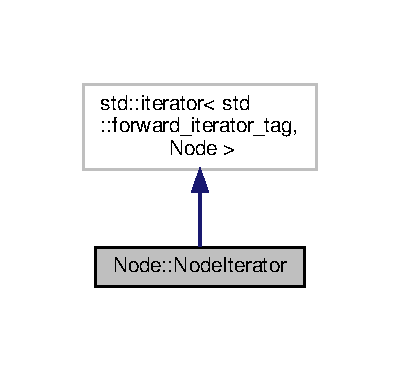
\includegraphics[width=192pt]{class_node_1_1_node_iterator__inherit__graph}
\end{center}
\end{figure}


Collaboration diagram for Node\+:\+:Node\+Iterator\+:\nopagebreak
\begin{figure}[H]
\begin{center}
\leavevmode
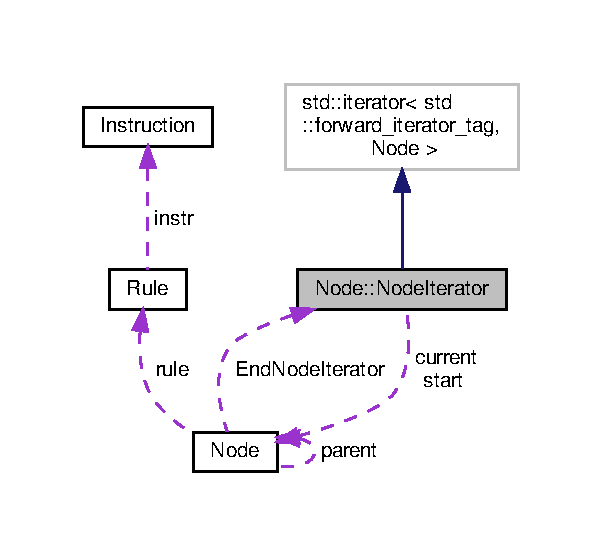
\includegraphics[width=289pt]{class_node_1_1_node_iterator__coll__graph}
\end{center}
\end{figure}
\subsection*{Public Member Functions}
\begin{DoxyCompactItemize}
\item 
\hyperlink{class_node_1_1_node_iterator_a6c8a582279465a5aa2d27bb9c0e71359}{Node\+Iterator} (const \hyperlink{class_node}{Node} $\ast$n)
\item 
\hyperlink{class_node}{Node} \& \hyperlink{class_node_1_1_node_iterator_a2b87cc748e7f197939e8d8b5a0e526ca}{operator$\ast$} () const
\item 
\hyperlink{class_node}{Node} $\ast$ \hyperlink{class_node_1_1_node_iterator_ab325945a6eccc93043b9fd35705529d9}{operator-\/$>$} () const
\item 
\hyperlink{class_node_1_1_node_iterator}{Node\+Iterator} \& \hyperlink{class_node_1_1_node_iterator_a13144818341346563030e7c0adab769c}{operator++} (int blah)
\item 
\hyperlink{class_node_1_1_node_iterator}{Node\+Iterator} \& \hyperlink{class_node_1_1_node_iterator_a906b69f8095b2e8e8ddfd68a40d9df48}{operator++} ()
\item 
\hyperlink{class_node_1_1_node_iterator}{Node\+Iterator} \& \hyperlink{class_node_1_1_node_iterator_a5ed6466d0f2200d90507769d4a790a9f}{operator+} (size\+\_\+t n)
\item 
bool \hyperlink{class_node_1_1_node_iterator_a5c01bff31ec6a91410c08ab70110cb1f}{operator==} (const \hyperlink{class_node_1_1_node_iterator}{Node\+Iterator} \&rhs)
\item 
bool \hyperlink{class_node_1_1_node_iterator_af76058ef35f25f3bcf681a4841554f58}{operator!=} (const \hyperlink{class_node_1_1_node_iterator}{Node\+Iterator} \&rhs)
\end{DoxyCompactItemize}
\subsection*{Protected Attributes}
\begin{DoxyCompactItemize}
\item 
\hyperlink{class_node}{Node} $\ast$ \hyperlink{class_node_1_1_node_iterator_aef4bbf58890919058172facd8b91238a}{current}
\item 
const \hyperlink{class_node}{Node} $\ast$ \hyperlink{class_node_1_1_node_iterator_a7f1dc14103049a99cd9929946ecbd0f0}{start}
\end{DoxyCompactItemize}


\subsection{Constructor \& Destructor Documentation}
\mbox{\Hypertarget{class_node_1_1_node_iterator_a6c8a582279465a5aa2d27bb9c0e71359}\label{class_node_1_1_node_iterator_a6c8a582279465a5aa2d27bb9c0e71359}} 
\index{Node\+::\+Node\+Iterator@{Node\+::\+Node\+Iterator}!Node\+Iterator@{Node\+Iterator}}
\index{Node\+Iterator@{Node\+Iterator}!Node\+::\+Node\+Iterator@{Node\+::\+Node\+Iterator}}
\subsubsection{\texorpdfstring{Node\+Iterator()}{NodeIterator()}}
{\footnotesize\ttfamily Node\+::\+Node\+Iterator\+::\+Node\+Iterator (\begin{DoxyParamCaption}\item[{const \hyperlink{class_node}{Node} $\ast$}]{n }\end{DoxyParamCaption})\hspace{0.3cm}{\ttfamily [inline]}}



\subsection{Member Function Documentation}
\mbox{\Hypertarget{class_node_1_1_node_iterator_af76058ef35f25f3bcf681a4841554f58}\label{class_node_1_1_node_iterator_af76058ef35f25f3bcf681a4841554f58}} 
\index{Node\+::\+Node\+Iterator@{Node\+::\+Node\+Iterator}!operator"!=@{operator"!=}}
\index{operator"!=@{operator"!=}!Node\+::\+Node\+Iterator@{Node\+::\+Node\+Iterator}}
\subsubsection{\texorpdfstring{operator"!=()}{operator!=()}}
{\footnotesize\ttfamily bool Node\+::\+Node\+Iterator\+::operator!= (\begin{DoxyParamCaption}\item[{const \hyperlink{class_node_1_1_node_iterator}{Node\+Iterator} \&}]{rhs }\end{DoxyParamCaption})\hspace{0.3cm}{\ttfamily [inline]}}

\mbox{\Hypertarget{class_node_1_1_node_iterator_a2b87cc748e7f197939e8d8b5a0e526ca}\label{class_node_1_1_node_iterator_a2b87cc748e7f197939e8d8b5a0e526ca}} 
\index{Node\+::\+Node\+Iterator@{Node\+::\+Node\+Iterator}!operator$\ast$@{operator$\ast$}}
\index{operator$\ast$@{operator$\ast$}!Node\+::\+Node\+Iterator@{Node\+::\+Node\+Iterator}}
\subsubsection{\texorpdfstring{operator$\ast$()}{operator*()}}
{\footnotesize\ttfamily \hyperlink{class_node}{Node}\& Node\+::\+Node\+Iterator\+::operator$\ast$ (\begin{DoxyParamCaption}{ }\end{DoxyParamCaption}) const\hspace{0.3cm}{\ttfamily [inline]}}

\mbox{\Hypertarget{class_node_1_1_node_iterator_a5ed6466d0f2200d90507769d4a790a9f}\label{class_node_1_1_node_iterator_a5ed6466d0f2200d90507769d4a790a9f}} 
\index{Node\+::\+Node\+Iterator@{Node\+::\+Node\+Iterator}!operator+@{operator+}}
\index{operator+@{operator+}!Node\+::\+Node\+Iterator@{Node\+::\+Node\+Iterator}}
\subsubsection{\texorpdfstring{operator+()}{operator+()}}
{\footnotesize\ttfamily \hyperlink{class_node_1_1_node_iterator}{Node\+Iterator}\& Node\+::\+Node\+Iterator\+::operator+ (\begin{DoxyParamCaption}\item[{size\+\_\+t}]{n }\end{DoxyParamCaption})\hspace{0.3cm}{\ttfamily [inline]}}

\mbox{\Hypertarget{class_node_1_1_node_iterator_a13144818341346563030e7c0adab769c}\label{class_node_1_1_node_iterator_a13144818341346563030e7c0adab769c}} 
\index{Node\+::\+Node\+Iterator@{Node\+::\+Node\+Iterator}!operator++@{operator++}}
\index{operator++@{operator++}!Node\+::\+Node\+Iterator@{Node\+::\+Node\+Iterator}}
\subsubsection{\texorpdfstring{operator++()}{operator++()}\hspace{0.1cm}{\footnotesize\ttfamily [1/2]}}
{\footnotesize\ttfamily \hyperlink{class_node_1_1_node_iterator}{Node\+Iterator}\& Node\+::\+Node\+Iterator\+::operator++ (\begin{DoxyParamCaption}\item[{int}]{blah }\end{DoxyParamCaption})\hspace{0.3cm}{\ttfamily [inline]}}

\mbox{\Hypertarget{class_node_1_1_node_iterator_a906b69f8095b2e8e8ddfd68a40d9df48}\label{class_node_1_1_node_iterator_a906b69f8095b2e8e8ddfd68a40d9df48}} 
\index{Node\+::\+Node\+Iterator@{Node\+::\+Node\+Iterator}!operator++@{operator++}}
\index{operator++@{operator++}!Node\+::\+Node\+Iterator@{Node\+::\+Node\+Iterator}}
\subsubsection{\texorpdfstring{operator++()}{operator++()}\hspace{0.1cm}{\footnotesize\ttfamily [2/2]}}
{\footnotesize\ttfamily \hyperlink{class_node_1_1_node_iterator}{Node\+Iterator}\& Node\+::\+Node\+Iterator\+::operator++ (\begin{DoxyParamCaption}{ }\end{DoxyParamCaption})\hspace{0.3cm}{\ttfamily [inline]}}

\mbox{\Hypertarget{class_node_1_1_node_iterator_ab325945a6eccc93043b9fd35705529d9}\label{class_node_1_1_node_iterator_ab325945a6eccc93043b9fd35705529d9}} 
\index{Node\+::\+Node\+Iterator@{Node\+::\+Node\+Iterator}!operator-\/$>$@{operator-\/$>$}}
\index{operator-\/$>$@{operator-\/$>$}!Node\+::\+Node\+Iterator@{Node\+::\+Node\+Iterator}}
\subsubsection{\texorpdfstring{operator-\/$>$()}{operator->()}}
{\footnotesize\ttfamily \hyperlink{class_node}{Node}$\ast$ Node\+::\+Node\+Iterator\+::operator-\/$>$ (\begin{DoxyParamCaption}{ }\end{DoxyParamCaption}) const\hspace{0.3cm}{\ttfamily [inline]}}

\mbox{\Hypertarget{class_node_1_1_node_iterator_a5c01bff31ec6a91410c08ab70110cb1f}\label{class_node_1_1_node_iterator_a5c01bff31ec6a91410c08ab70110cb1f}} 
\index{Node\+::\+Node\+Iterator@{Node\+::\+Node\+Iterator}!operator==@{operator==}}
\index{operator==@{operator==}!Node\+::\+Node\+Iterator@{Node\+::\+Node\+Iterator}}
\subsubsection{\texorpdfstring{operator==()}{operator==()}}
{\footnotesize\ttfamily bool Node\+::\+Node\+Iterator\+::operator== (\begin{DoxyParamCaption}\item[{const \hyperlink{class_node_1_1_node_iterator}{Node\+Iterator} \&}]{rhs }\end{DoxyParamCaption})\hspace{0.3cm}{\ttfamily [inline]}}



\subsection{Member Data Documentation}
\mbox{\Hypertarget{class_node_1_1_node_iterator_aef4bbf58890919058172facd8b91238a}\label{class_node_1_1_node_iterator_aef4bbf58890919058172facd8b91238a}} 
\index{Node\+::\+Node\+Iterator@{Node\+::\+Node\+Iterator}!current@{current}}
\index{current@{current}!Node\+::\+Node\+Iterator@{Node\+::\+Node\+Iterator}}
\subsubsection{\texorpdfstring{current}{current}}
{\footnotesize\ttfamily \hyperlink{class_node}{Node}$\ast$ Node\+::\+Node\+Iterator\+::current\hspace{0.3cm}{\ttfamily [protected]}}

\mbox{\Hypertarget{class_node_1_1_node_iterator_a7f1dc14103049a99cd9929946ecbd0f0}\label{class_node_1_1_node_iterator_a7f1dc14103049a99cd9929946ecbd0f0}} 
\index{Node\+::\+Node\+Iterator@{Node\+::\+Node\+Iterator}!start@{start}}
\index{start@{start}!Node\+::\+Node\+Iterator@{Node\+::\+Node\+Iterator}}
\subsubsection{\texorpdfstring{start}{start}}
{\footnotesize\ttfamily const \hyperlink{class_node}{Node}$\ast$ Node\+::\+Node\+Iterator\+::start\hspace{0.3cm}{\ttfamily [protected]}}



The documentation for this class was generated from the following file\+:\begin{DoxyCompactItemize}
\item 
src/\hyperlink{_node_8h}{Node.\+h}\end{DoxyCompactItemize}

\hypertarget{struct_object}{}\section{Object Struct Reference}
\label{struct_object}\index{Object@{Object}}
\subsection*{Public Attributes}
\begin{DoxyCompactItemize}
\item 
\hyperlink{_rational_rules_2_main_8cpp_ab87bacfdad76e61b9412d7124be44c1c}{Color} \hyperlink{struct_object_a3ed85d6e0b0b62ff2501d421cb55c5e9}{color}
\item 
\hyperlink{_rational_rules_2_main_8cpp_a55b506070847a13554f8b879c1bfb37c}{Shape} \hyperlink{struct_object_a09a35e7356709e994637bd66c2c69fc4}{shape}
\end{DoxyCompactItemize}


\subsection{Member Data Documentation}
\mbox{\Hypertarget{struct_object_a3ed85d6e0b0b62ff2501d421cb55c5e9}\label{struct_object_a3ed85d6e0b0b62ff2501d421cb55c5e9}} 
\index{Object@{Object}!color@{color}}
\index{color@{color}!Object@{Object}}
\subsubsection{\texorpdfstring{color}{color}}
{\footnotesize\ttfamily \hyperlink{_rational_rules_2_main_8cpp_ab87bacfdad76e61b9412d7124be44c1c}{Color} Object\+::color}

\mbox{\Hypertarget{struct_object_a09a35e7356709e994637bd66c2c69fc4}\label{struct_object_a09a35e7356709e994637bd66c2c69fc4}} 
\index{Object@{Object}!shape@{shape}}
\index{shape@{shape}!Object@{Object}}
\subsubsection{\texorpdfstring{shape}{shape}}
{\footnotesize\ttfamily \hyperlink{_rational_rules_2_main_8cpp_a55b506070847a13554f8b879c1bfb37c}{Shape} Object\+::shape}



The documentation for this struct was generated from the following file\+:\begin{DoxyCompactItemize}
\item 
Models/\+Rational\+Rules/\hyperlink{_rational_rules_2_main_8cpp}{Main.\+cpp}\end{DoxyCompactItemize}

\hypertarget{class_parallel_tempering}{}\section{Parallel\+Tempering$<$ H\+YP, callback\+\_\+t $>$ Class Template Reference}
\label{class_parallel_tempering}\index{Parallel\+Tempering$<$ H\+Y\+P, callback\+\_\+t $>$@{Parallel\+Tempering$<$ H\+Y\+P, callback\+\_\+t $>$}}


{\ttfamily \#include $<$Parallel\+Tempering.\+h$>$}



Inheritance diagram for Parallel\+Tempering$<$ H\+YP, callback\+\_\+t $>$\+:\nopagebreak
\begin{figure}[H]
\begin{center}
\leavevmode
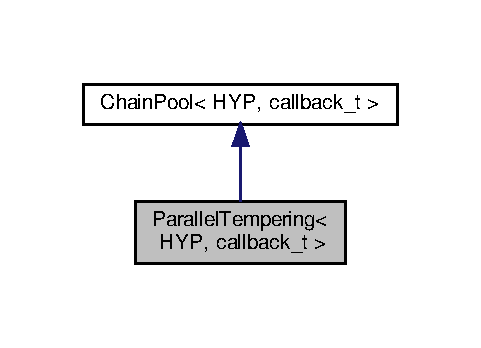
\includegraphics[width=231pt]{class_parallel_tempering__inherit__graph}
\end{center}
\end{figure}


Collaboration diagram for Parallel\+Tempering$<$ H\+YP, callback\+\_\+t $>$\+:\nopagebreak
\begin{figure}[H]
\begin{center}
\leavevmode
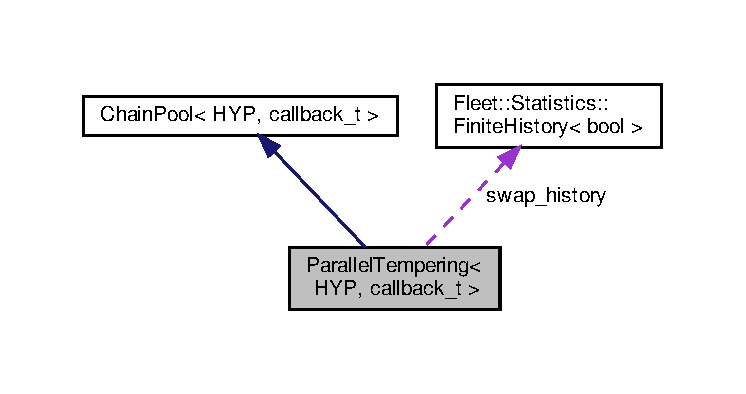
\includegraphics[width=350pt]{class_parallel_tempering__coll__graph}
\end{center}
\end{figure}
\subsection*{Public Member Functions}
\begin{DoxyCompactItemize}
\item 
\hyperlink{class_parallel_tempering_abac520918d0d6915c61d9595a82b01eb}{Parallel\+Tempering} (H\+YP \&h0, typename H\+Y\+P\+::t\+\_\+data $\ast$d, callback\+\_\+t \&cb, std\+::initializer\+\_\+list$<$ double $>$ t, bool allcallback=true)
\item 
\hyperlink{class_parallel_tempering_a6318b222a7fbc7148ce82d0bbc5a3ecd}{Parallel\+Tempering} (H\+YP \&h0, typename H\+Y\+P\+::t\+\_\+data $\ast$d, callback\+\_\+t \&cb, unsigned long n, double maxT, bool allcallback=true)
\item 
\hyperlink{class_parallel_tempering_ad4b72862bcc821fe725ac2248c150898}{Parallel\+Tempering} (H\+YP \&h0, std\+::vector$<$ typename H\+Y\+P\+::t\+\_\+data $>$ \&datas, std\+::vector$<$ callback\+\_\+t $>$ \&cb)
\item 
\hyperlink{class_parallel_tempering_a96763c107a95f4a120f2b65c896cb5b2}{$\sim$\+Parallel\+Tempering} ()
\item 
void \hyperlink{class_parallel_tempering_aa704d462a41cb45b461b967a97dedcbb}{\+\_\+\+\_\+swapper\+\_\+thread} (time\+\_\+ms swap\+\_\+every)
\item 
void \hyperlink{class_parallel_tempering_a6ae6bd8581ec13aad5983886b1a739e6}{\+\_\+\+\_\+adapter\+\_\+thread} (time\+\_\+ms adapt\+\_\+every)
\item 
virtual void \hyperlink{class_parallel_tempering_a6824837893cf52eb1cac362e78e483b9}{run} (\hyperlink{struct_control}{Control} ctl) override
\item 
virtual void \hyperlink{class_parallel_tempering_a40df4781b1d06acff7b0902c4d4a5a87}{run} (\hyperlink{struct_control}{Control} ctl, time\+\_\+ms swap\+\_\+every, time\+\_\+ms adapt\+\_\+every)
\item 
void \hyperlink{class_parallel_tempering_a9e1960158b12a4dadfab54eb4fb895d3}{show\+\_\+statistics} ()
\item 
double \hyperlink{class_parallel_tempering_a439c50d3f616319803d4ab83804d1ae0}{k} (unsigned long t, double v, double t0)
\item 
void \hyperlink{class_parallel_tempering_a673feff316b65cad63f56ceb81b128ae}{adapt} (double v=3, double t0=1000000)
\end{DoxyCompactItemize}
\subsection*{Public Attributes}
\begin{DoxyCompactItemize}
\item 
std\+::vector$<$ double $>$ \hyperlink{class_parallel_tempering_a5aca1e6ca522986f183d61c91c94d21d}{temperatures}
\item 
\hyperlink{class_fleet_1_1_statistics_1_1_finite_history}{Fleet\+::\+Statistics\+::\+Finite\+History}$<$ bool $>$ $\ast$ \hyperlink{class_parallel_tempering_a86a7b77250a04b5df502f1c770cf51bf}{swap\+\_\+history}
\item 
bool \hyperlink{class_parallel_tempering_ae9f0a2af938df838cc4010983860394e}{is\+\_\+temperature}
\item 
std\+::atomic$<$ bool $>$ \hyperlink{class_parallel_tempering_acda523b375468743e7d8ac471af65285}{terminate}
\end{DoxyCompactItemize}
\subsection*{Additional Inherited Members}


\subsection{Constructor \& Destructor Documentation}
\mbox{\Hypertarget{class_parallel_tempering_abac520918d0d6915c61d9595a82b01eb}\label{class_parallel_tempering_abac520918d0d6915c61d9595a82b01eb}} 
\index{Parallel\+Tempering@{Parallel\+Tempering}!Parallel\+Tempering@{Parallel\+Tempering}}
\index{Parallel\+Tempering@{Parallel\+Tempering}!Parallel\+Tempering@{Parallel\+Tempering}}
\subsubsection{\texorpdfstring{Parallel\+Tempering()}{ParallelTempering()}\hspace{0.1cm}{\footnotesize\ttfamily [1/3]}}
{\footnotesize\ttfamily template$<$typename H\+YP , typename callback\+\_\+t $>$ \\
\hyperlink{class_parallel_tempering}{Parallel\+Tempering}$<$ H\+YP, callback\+\_\+t $>$\+::\hyperlink{class_parallel_tempering}{Parallel\+Tempering} (\begin{DoxyParamCaption}\item[{H\+YP \&}]{h0,  }\item[{typename H\+Y\+P\+::t\+\_\+data $\ast$}]{d,  }\item[{callback\+\_\+t \&}]{cb,  }\item[{std\+::initializer\+\_\+list$<$ double $>$}]{t,  }\item[{bool}]{allcallback = {\ttfamily true} }\end{DoxyParamCaption})\hspace{0.3cm}{\ttfamily [inline]}}

\mbox{\Hypertarget{class_parallel_tempering_a6318b222a7fbc7148ce82d0bbc5a3ecd}\label{class_parallel_tempering_a6318b222a7fbc7148ce82d0bbc5a3ecd}} 
\index{Parallel\+Tempering@{Parallel\+Tempering}!Parallel\+Tempering@{Parallel\+Tempering}}
\index{Parallel\+Tempering@{Parallel\+Tempering}!Parallel\+Tempering@{Parallel\+Tempering}}
\subsubsection{\texorpdfstring{Parallel\+Tempering()}{ParallelTempering()}\hspace{0.1cm}{\footnotesize\ttfamily [2/3]}}
{\footnotesize\ttfamily template$<$typename H\+YP , typename callback\+\_\+t $>$ \\
\hyperlink{class_parallel_tempering}{Parallel\+Tempering}$<$ H\+YP, callback\+\_\+t $>$\+::\hyperlink{class_parallel_tempering}{Parallel\+Tempering} (\begin{DoxyParamCaption}\item[{H\+YP \&}]{h0,  }\item[{typename H\+Y\+P\+::t\+\_\+data $\ast$}]{d,  }\item[{callback\+\_\+t \&}]{cb,  }\item[{unsigned long}]{n,  }\item[{double}]{maxT,  }\item[{bool}]{allcallback = {\ttfamily true} }\end{DoxyParamCaption})\hspace{0.3cm}{\ttfamily [inline]}}

\mbox{\Hypertarget{class_parallel_tempering_ad4b72862bcc821fe725ac2248c150898}\label{class_parallel_tempering_ad4b72862bcc821fe725ac2248c150898}} 
\index{Parallel\+Tempering@{Parallel\+Tempering}!Parallel\+Tempering@{Parallel\+Tempering}}
\index{Parallel\+Tempering@{Parallel\+Tempering}!Parallel\+Tempering@{Parallel\+Tempering}}
\subsubsection{\texorpdfstring{Parallel\+Tempering()}{ParallelTempering()}\hspace{0.1cm}{\footnotesize\ttfamily [3/3]}}
{\footnotesize\ttfamily template$<$typename H\+YP , typename callback\+\_\+t $>$ \\
\hyperlink{class_parallel_tempering}{Parallel\+Tempering}$<$ H\+YP, callback\+\_\+t $>$\+::\hyperlink{class_parallel_tempering}{Parallel\+Tempering} (\begin{DoxyParamCaption}\item[{H\+YP \&}]{h0,  }\item[{std\+::vector$<$ typename H\+Y\+P\+::t\+\_\+data $>$ \&}]{datas,  }\item[{std\+::vector$<$ callback\+\_\+t $>$ \&}]{cb }\end{DoxyParamCaption})\hspace{0.3cm}{\ttfamily [inline]}}

\mbox{\Hypertarget{class_parallel_tempering_a96763c107a95f4a120f2b65c896cb5b2}\label{class_parallel_tempering_a96763c107a95f4a120f2b65c896cb5b2}} 
\index{Parallel\+Tempering@{Parallel\+Tempering}!````~Parallel\+Tempering@{$\sim$\+Parallel\+Tempering}}
\index{````~Parallel\+Tempering@{$\sim$\+Parallel\+Tempering}!Parallel\+Tempering@{Parallel\+Tempering}}
\subsubsection{\texorpdfstring{$\sim$\+Parallel\+Tempering()}{~ParallelTempering()}}
{\footnotesize\ttfamily template$<$typename H\+YP , typename callback\+\_\+t $>$ \\
\hyperlink{class_parallel_tempering}{Parallel\+Tempering}$<$ H\+YP, callback\+\_\+t $>$\+::$\sim$\hyperlink{class_parallel_tempering}{Parallel\+Tempering} (\begin{DoxyParamCaption}{ }\end{DoxyParamCaption})\hspace{0.3cm}{\ttfamily [inline]}}



\subsection{Member Function Documentation}
\mbox{\Hypertarget{class_parallel_tempering_a6ae6bd8581ec13aad5983886b1a739e6}\label{class_parallel_tempering_a6ae6bd8581ec13aad5983886b1a739e6}} 
\index{Parallel\+Tempering@{Parallel\+Tempering}!\+\_\+\+\_\+adapter\+\_\+thread@{\+\_\+\+\_\+adapter\+\_\+thread}}
\index{\+\_\+\+\_\+adapter\+\_\+thread@{\+\_\+\+\_\+adapter\+\_\+thread}!Parallel\+Tempering@{Parallel\+Tempering}}
\subsubsection{\texorpdfstring{\+\_\+\+\_\+adapter\+\_\+thread()}{\_\_adapter\_thread()}}
{\footnotesize\ttfamily template$<$typename H\+YP , typename callback\+\_\+t $>$ \\
void \hyperlink{class_parallel_tempering}{Parallel\+Tempering}$<$ H\+YP, callback\+\_\+t $>$\+::\+\_\+\+\_\+adapter\+\_\+thread (\begin{DoxyParamCaption}\item[{time\+\_\+ms}]{adapt\+\_\+every }\end{DoxyParamCaption})\hspace{0.3cm}{\ttfamily [inline]}}

\mbox{\Hypertarget{class_parallel_tempering_aa704d462a41cb45b461b967a97dedcbb}\label{class_parallel_tempering_aa704d462a41cb45b461b967a97dedcbb}} 
\index{Parallel\+Tempering@{Parallel\+Tempering}!\+\_\+\+\_\+swapper\+\_\+thread@{\+\_\+\+\_\+swapper\+\_\+thread}}
\index{\+\_\+\+\_\+swapper\+\_\+thread@{\+\_\+\+\_\+swapper\+\_\+thread}!Parallel\+Tempering@{Parallel\+Tempering}}
\subsubsection{\texorpdfstring{\+\_\+\+\_\+swapper\+\_\+thread()}{\_\_swapper\_thread()}}
{\footnotesize\ttfamily template$<$typename H\+YP , typename callback\+\_\+t $>$ \\
void \hyperlink{class_parallel_tempering}{Parallel\+Tempering}$<$ H\+YP, callback\+\_\+t $>$\+::\+\_\+\+\_\+swapper\+\_\+thread (\begin{DoxyParamCaption}\item[{time\+\_\+ms}]{swap\+\_\+every }\end{DoxyParamCaption})\hspace{0.3cm}{\ttfamily [inline]}}

\mbox{\Hypertarget{class_parallel_tempering_a673feff316b65cad63f56ceb81b128ae}\label{class_parallel_tempering_a673feff316b65cad63f56ceb81b128ae}} 
\index{Parallel\+Tempering@{Parallel\+Tempering}!adapt@{adapt}}
\index{adapt@{adapt}!Parallel\+Tempering@{Parallel\+Tempering}}
\subsubsection{\texorpdfstring{adapt()}{adapt()}}
{\footnotesize\ttfamily template$<$typename H\+YP , typename callback\+\_\+t $>$ \\
void \hyperlink{class_parallel_tempering}{Parallel\+Tempering}$<$ H\+YP, callback\+\_\+t $>$\+::adapt (\begin{DoxyParamCaption}\item[{double}]{v = {\ttfamily 3},  }\item[{double}]{t0 = {\ttfamily 1000000} }\end{DoxyParamCaption})\hspace{0.3cm}{\ttfamily [inline]}}

\mbox{\Hypertarget{class_parallel_tempering_a439c50d3f616319803d4ab83804d1ae0}\label{class_parallel_tempering_a439c50d3f616319803d4ab83804d1ae0}} 
\index{Parallel\+Tempering@{Parallel\+Tempering}!k@{k}}
\index{k@{k}!Parallel\+Tempering@{Parallel\+Tempering}}
\subsubsection{\texorpdfstring{k()}{k()}}
{\footnotesize\ttfamily template$<$typename H\+YP , typename callback\+\_\+t $>$ \\
double \hyperlink{class_parallel_tempering}{Parallel\+Tempering}$<$ H\+YP, callback\+\_\+t $>$\+::k (\begin{DoxyParamCaption}\item[{unsigned long}]{t,  }\item[{double}]{v,  }\item[{double}]{t0 }\end{DoxyParamCaption})\hspace{0.3cm}{\ttfamily [inline]}}

\mbox{\Hypertarget{class_parallel_tempering_a6824837893cf52eb1cac362e78e483b9}\label{class_parallel_tempering_a6824837893cf52eb1cac362e78e483b9}} 
\index{Parallel\+Tempering@{Parallel\+Tempering}!run@{run}}
\index{run@{run}!Parallel\+Tempering@{Parallel\+Tempering}}
\subsubsection{\texorpdfstring{run()}{run()}\hspace{0.1cm}{\footnotesize\ttfamily [1/2]}}
{\footnotesize\ttfamily template$<$typename H\+YP , typename callback\+\_\+t $>$ \\
virtual void \hyperlink{class_parallel_tempering}{Parallel\+Tempering}$<$ H\+YP, callback\+\_\+t $>$\+::run (\begin{DoxyParamCaption}\item[{\hyperlink{struct_control}{Control}}]{ctl }\end{DoxyParamCaption})\hspace{0.3cm}{\ttfamily [inline]}, {\ttfamily [override]}, {\ttfamily [virtual]}}



Reimplemented from \hyperlink{class_chain_pool_af5f0e391f9794ff89f29296c8b41bf8e}{Chain\+Pool$<$ H\+Y\+P, callback\+\_\+t $>$}.

\mbox{\Hypertarget{class_parallel_tempering_a40df4781b1d06acff7b0902c4d4a5a87}\label{class_parallel_tempering_a40df4781b1d06acff7b0902c4d4a5a87}} 
\index{Parallel\+Tempering@{Parallel\+Tempering}!run@{run}}
\index{run@{run}!Parallel\+Tempering@{Parallel\+Tempering}}
\subsubsection{\texorpdfstring{run()}{run()}\hspace{0.1cm}{\footnotesize\ttfamily [2/2]}}
{\footnotesize\ttfamily template$<$typename H\+YP , typename callback\+\_\+t $>$ \\
virtual void \hyperlink{class_parallel_tempering}{Parallel\+Tempering}$<$ H\+YP, callback\+\_\+t $>$\+::run (\begin{DoxyParamCaption}\item[{\hyperlink{struct_control}{Control}}]{ctl,  }\item[{time\+\_\+ms}]{swap\+\_\+every,  }\item[{time\+\_\+ms}]{adapt\+\_\+every }\end{DoxyParamCaption})\hspace{0.3cm}{\ttfamily [inline]}, {\ttfamily [virtual]}}

\mbox{\Hypertarget{class_parallel_tempering_a9e1960158b12a4dadfab54eb4fb895d3}\label{class_parallel_tempering_a9e1960158b12a4dadfab54eb4fb895d3}} 
\index{Parallel\+Tempering@{Parallel\+Tempering}!show\+\_\+statistics@{show\+\_\+statistics}}
\index{show\+\_\+statistics@{show\+\_\+statistics}!Parallel\+Tempering@{Parallel\+Tempering}}
\subsubsection{\texorpdfstring{show\+\_\+statistics()}{show\_statistics()}}
{\footnotesize\ttfamily template$<$typename H\+YP , typename callback\+\_\+t $>$ \\
void \hyperlink{class_parallel_tempering}{Parallel\+Tempering}$<$ H\+YP, callback\+\_\+t $>$\+::show\+\_\+statistics (\begin{DoxyParamCaption}{ }\end{DoxyParamCaption})\hspace{0.3cm}{\ttfamily [inline]}}



\subsection{Member Data Documentation}
\mbox{\Hypertarget{class_parallel_tempering_ae9f0a2af938df838cc4010983860394e}\label{class_parallel_tempering_ae9f0a2af938df838cc4010983860394e}} 
\index{Parallel\+Tempering@{Parallel\+Tempering}!is\+\_\+temperature@{is\+\_\+temperature}}
\index{is\+\_\+temperature@{is\+\_\+temperature}!Parallel\+Tempering@{Parallel\+Tempering}}
\subsubsection{\texorpdfstring{is\+\_\+temperature}{is\_temperature}}
{\footnotesize\ttfamily template$<$typename H\+YP , typename callback\+\_\+t $>$ \\
bool \hyperlink{class_parallel_tempering}{Parallel\+Tempering}$<$ H\+YP, callback\+\_\+t $>$\+::is\+\_\+temperature}

\mbox{\Hypertarget{class_parallel_tempering_a86a7b77250a04b5df502f1c770cf51bf}\label{class_parallel_tempering_a86a7b77250a04b5df502f1c770cf51bf}} 
\index{Parallel\+Tempering@{Parallel\+Tempering}!swap\+\_\+history@{swap\+\_\+history}}
\index{swap\+\_\+history@{swap\+\_\+history}!Parallel\+Tempering@{Parallel\+Tempering}}
\subsubsection{\texorpdfstring{swap\+\_\+history}{swap\_history}}
{\footnotesize\ttfamily template$<$typename H\+YP , typename callback\+\_\+t $>$ \\
\hyperlink{class_fleet_1_1_statistics_1_1_finite_history}{Fleet\+::\+Statistics\+::\+Finite\+History}$<$bool$>$$\ast$ \hyperlink{class_parallel_tempering}{Parallel\+Tempering}$<$ H\+YP, callback\+\_\+t $>$\+::swap\+\_\+history}

\mbox{\Hypertarget{class_parallel_tempering_a5aca1e6ca522986f183d61c91c94d21d}\label{class_parallel_tempering_a5aca1e6ca522986f183d61c91c94d21d}} 
\index{Parallel\+Tempering@{Parallel\+Tempering}!temperatures@{temperatures}}
\index{temperatures@{temperatures}!Parallel\+Tempering@{Parallel\+Tempering}}
\subsubsection{\texorpdfstring{temperatures}{temperatures}}
{\footnotesize\ttfamily template$<$typename H\+YP , typename callback\+\_\+t $>$ \\
std\+::vector$<$double$>$ \hyperlink{class_parallel_tempering}{Parallel\+Tempering}$<$ H\+YP, callback\+\_\+t $>$\+::temperatures}

\mbox{\Hypertarget{class_parallel_tempering_acda523b375468743e7d8ac471af65285}\label{class_parallel_tempering_acda523b375468743e7d8ac471af65285}} 
\index{Parallel\+Tempering@{Parallel\+Tempering}!terminate@{terminate}}
\index{terminate@{terminate}!Parallel\+Tempering@{Parallel\+Tempering}}
\subsubsection{\texorpdfstring{terminate}{terminate}}
{\footnotesize\ttfamily template$<$typename H\+YP , typename callback\+\_\+t $>$ \\
std\+::atomic$<$bool$>$ \hyperlink{class_parallel_tempering}{Parallel\+Tempering}$<$ H\+YP, callback\+\_\+t $>$\+::terminate}



The documentation for this class was generated from the following file\+:\begin{DoxyCompactItemize}
\item 
src/\+Inference/\hyperlink{_parallel_tempering_8h}{Parallel\+Tempering.\+h}\end{DoxyCompactItemize}

\hypertarget{struct_pre_primitive}{}\section{Pre\+Primitive Struct Reference}
\label{struct_pre_primitive}\index{Pre\+Primitive@{Pre\+Primitive}}


{\ttfamily \#include $<$Primitives.\+h$>$}



Inheritance diagram for Pre\+Primitive\+:\nopagebreak
\begin{figure}[H]
\begin{center}
\leavevmode
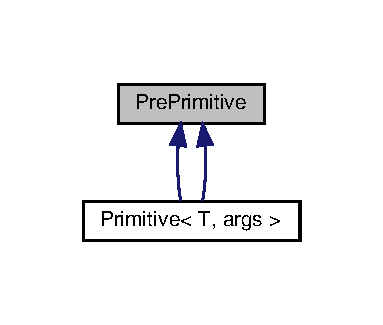
\includegraphics[width=184pt]{struct_pre_primitive__inherit__graph}
\end{center}
\end{figure}


Collaboration diagram for Pre\+Primitive\+:\nopagebreak
\begin{figure}[H]
\begin{center}
\leavevmode
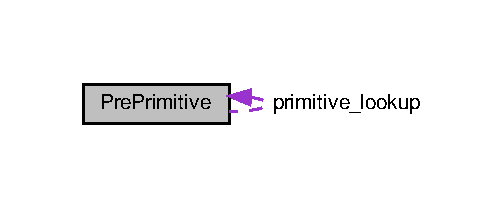
\includegraphics[width=242pt]{struct_pre_primitive__coll__graph}
\end{center}
\end{figure}
\subsection*{Public Member Functions}
\begin{DoxyCompactItemize}
\item 
\hyperlink{struct_pre_primitive_a8a96c30ad34b1f19f0539eea4d0423f6}{Pre\+Primitive} ()
\end{DoxyCompactItemize}
\subsection*{Public Attributes}
\begin{DoxyCompactItemize}
\item 
const \hyperlink{_instruction_8h_a227278394efd1e2313c727102db09ea9}{Primitive\+Op} \hyperlink{struct_pre_primitive_a209912eb2296e524388fa1f83e7d834b}{op}
\end{DoxyCompactItemize}
\subsection*{Static Public Attributes}
\begin{DoxyCompactItemize}
\item 
static \hyperlink{_instruction_8h_a227278394efd1e2313c727102db09ea9}{Primitive\+Op} \hyperlink{struct_pre_primitive_a8f4088dc0a3fe00fd81c509bb0af1881}{op\+\_\+counter} = 0
\item 
static \hyperlink{_instruction_8h_a227278394efd1e2313c727102db09ea9}{Primitive\+Op} \hyperlink{struct_pre_primitive_a42ca9726dd60d24f8148e766d5e8ecc8}{global\+\_\+primitive\+\_\+counter} = 0
\item 
static const size\+\_\+t \hyperlink{struct_pre_primitive_aaa931d0f215c4a79ab4920c13a82a32b}{M\+A\+X\+\_\+\+P\+R\+I\+M\+I\+T\+I\+V\+ES} = 256
\item 
static \hyperlink{struct_pre_primitive}{Pre\+Primitive} $\ast$ \hyperlink{struct_pre_primitive_a286cab59ea91d634e75f435cd9812dd1}{primitive\+\_\+lookup} \mbox{[}\hyperlink{struct_pre_primitive_aaa931d0f215c4a79ab4920c13a82a32b}{M\+A\+X\+\_\+\+P\+R\+I\+M\+I\+T\+I\+V\+ES}\mbox{]}
\end{DoxyCompactItemize}


\subsection{Constructor \& Destructor Documentation}
\mbox{\Hypertarget{struct_pre_primitive_a8a96c30ad34b1f19f0539eea4d0423f6}\label{struct_pre_primitive_a8a96c30ad34b1f19f0539eea4d0423f6}} 
\index{Pre\+Primitive@{Pre\+Primitive}!Pre\+Primitive@{Pre\+Primitive}}
\index{Pre\+Primitive@{Pre\+Primitive}!Pre\+Primitive@{Pre\+Primitive}}
\subsubsection{\texorpdfstring{Pre\+Primitive()}{PrePrimitive()}}
{\footnotesize\ttfamily Pre\+Primitive\+::\+Pre\+Primitive (\begin{DoxyParamCaption}{ }\end{DoxyParamCaption})\hspace{0.3cm}{\ttfamily [inline]}}



\subsection{Member Data Documentation}
\mbox{\Hypertarget{struct_pre_primitive_a42ca9726dd60d24f8148e766d5e8ecc8}\label{struct_pre_primitive_a42ca9726dd60d24f8148e766d5e8ecc8}} 
\index{Pre\+Primitive@{Pre\+Primitive}!global\+\_\+primitive\+\_\+counter@{global\+\_\+primitive\+\_\+counter}}
\index{global\+\_\+primitive\+\_\+counter@{global\+\_\+primitive\+\_\+counter}!Pre\+Primitive@{Pre\+Primitive}}
\subsubsection{\texorpdfstring{global\+\_\+primitive\+\_\+counter}{global\_primitive\_counter}}
{\footnotesize\ttfamily \hyperlink{_instruction_8h_a227278394efd1e2313c727102db09ea9}{Primitive\+Op} Pre\+Primitive\+::global\+\_\+primitive\+\_\+counter = 0\hspace{0.3cm}{\ttfamily [static]}}

\mbox{\Hypertarget{struct_pre_primitive_aaa931d0f215c4a79ab4920c13a82a32b}\label{struct_pre_primitive_aaa931d0f215c4a79ab4920c13a82a32b}} 
\index{Pre\+Primitive@{Pre\+Primitive}!M\+A\+X\+\_\+\+P\+R\+I\+M\+I\+T\+I\+V\+ES@{M\+A\+X\+\_\+\+P\+R\+I\+M\+I\+T\+I\+V\+ES}}
\index{M\+A\+X\+\_\+\+P\+R\+I\+M\+I\+T\+I\+V\+ES@{M\+A\+X\+\_\+\+P\+R\+I\+M\+I\+T\+I\+V\+ES}!Pre\+Primitive@{Pre\+Primitive}}
\subsubsection{\texorpdfstring{M\+A\+X\+\_\+\+P\+R\+I\+M\+I\+T\+I\+V\+ES}{MAX\_PRIMITIVES}}
{\footnotesize\ttfamily const size\+\_\+t Pre\+Primitive\+::\+M\+A\+X\+\_\+\+P\+R\+I\+M\+I\+T\+I\+V\+ES = 256\hspace{0.3cm}{\ttfamily [static]}}

\mbox{\Hypertarget{struct_pre_primitive_a209912eb2296e524388fa1f83e7d834b}\label{struct_pre_primitive_a209912eb2296e524388fa1f83e7d834b}} 
\index{Pre\+Primitive@{Pre\+Primitive}!op@{op}}
\index{op@{op}!Pre\+Primitive@{Pre\+Primitive}}
\subsubsection{\texorpdfstring{op}{op}}
{\footnotesize\ttfamily const \hyperlink{_instruction_8h_a227278394efd1e2313c727102db09ea9}{Primitive\+Op} Pre\+Primitive\+::op}

\mbox{\Hypertarget{struct_pre_primitive_a8f4088dc0a3fe00fd81c509bb0af1881}\label{struct_pre_primitive_a8f4088dc0a3fe00fd81c509bb0af1881}} 
\index{Pre\+Primitive@{Pre\+Primitive}!op\+\_\+counter@{op\+\_\+counter}}
\index{op\+\_\+counter@{op\+\_\+counter}!Pre\+Primitive@{Pre\+Primitive}}
\subsubsection{\texorpdfstring{op\+\_\+counter}{op\_counter}}
{\footnotesize\ttfamily \hyperlink{_instruction_8h_a227278394efd1e2313c727102db09ea9}{Primitive\+Op} Pre\+Primitive\+::op\+\_\+counter = 0\hspace{0.3cm}{\ttfamily [static]}}

\mbox{\Hypertarget{struct_pre_primitive_a286cab59ea91d634e75f435cd9812dd1}\label{struct_pre_primitive_a286cab59ea91d634e75f435cd9812dd1}} 
\index{Pre\+Primitive@{Pre\+Primitive}!primitive\+\_\+lookup@{primitive\+\_\+lookup}}
\index{primitive\+\_\+lookup@{primitive\+\_\+lookup}!Pre\+Primitive@{Pre\+Primitive}}
\subsubsection{\texorpdfstring{primitive\+\_\+lookup}{primitive\_lookup}}
{\footnotesize\ttfamily \hyperlink{struct_pre_primitive}{Pre\+Primitive}$\ast$ Pre\+Primitive\+::primitive\+\_\+lookup\mbox{[}\hyperlink{struct_pre_primitive_aaa931d0f215c4a79ab4920c13a82a32b}{M\+A\+X\+\_\+\+P\+R\+I\+M\+I\+T\+I\+V\+ES}\mbox{]}\hspace{0.3cm}{\ttfamily [static]}}



The documentation for this struct was generated from the following files\+:\begin{DoxyCompactItemize}
\item 
src/\+Virtual\+Machine/\hyperlink{_primitives_8h}{Primitives.\+h}\item 
src/\+Virtual\+Machine/\hyperlink{_primitives2_8h}{Primitives2.\+h}\end{DoxyCompactItemize}

\hypertarget{struct_primitive}{}\section{Primitive$<$ T, args $>$ Class Template Reference}
\label{struct_primitive}\index{Primitive$<$ T, args $>$@{Primitive$<$ T, args $>$}}


{\ttfamily \#include $<$Grammar.\+h$>$}



Inheritance diagram for Primitive$<$ T, args $>$\+:\nopagebreak
\begin{figure}[H]
\begin{center}
\leavevmode
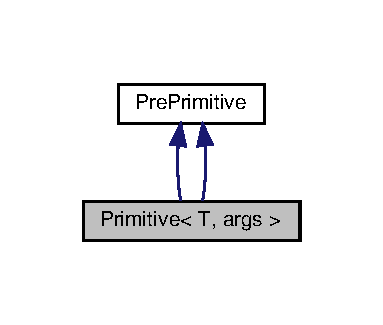
\includegraphics[width=184pt]{struct_primitive__inherit__graph}
\end{center}
\end{figure}


Collaboration diagram for Primitive$<$ T, args $>$\+:\nopagebreak
\begin{figure}[H]
\begin{center}
\leavevmode
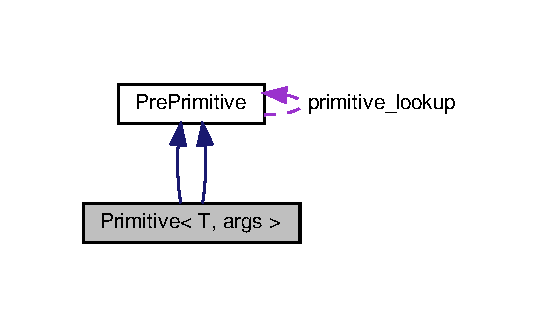
\includegraphics[width=259pt]{struct_primitive__coll__graph}
\end{center}
\end{figure}
\subsection*{Public Types}
\begin{DoxyCompactItemize}
\item 
typedef std\+::decay$<$ typename Head\+If\+Reference\+ElseT$<$ T, args... $>$\+::type $>$\+::type \hyperlink{struct_primitive_a1f2d2db3fb7869d03d65112e30d22101}{Grammar\+Return\+Type}
\item 
typedef std\+::decay$<$ typename Head\+If\+Reference\+ElseT$<$ T, args... $>$\+::type $>$\+::type \hyperlink{struct_primitive_a1f2d2db3fb7869d03d65112e30d22101}{Grammar\+Return\+Type}
\end{DoxyCompactItemize}
\subsection*{Public Member Functions}
\begin{DoxyCompactItemize}
\item 
\hyperlink{struct_primitive_a4303c3567a7bb2921d298f48b07b0add}{Primitive} (std\+::string fmt, T($\ast$f)(args...), double \+\_\+p=1.\+0)
\item 
{\footnotesize template$<$typename V , typename P , typename L $>$ }\\\hyperlink{_instruction_8h_a6202215407ab29590bb936ca2996cf64}{vmstatus\+\_\+t} \hyperlink{struct_primitive_a10cedec90ed4a3ff01be2bd3b9c36528}{V\+M\+Scall} (V $\ast$vms, P $\ast$pool, L $\ast$loader)
\begin{DoxyCompactList}\small\item\em This gets called by a \hyperlink{class_virtual_machine_state}{Virtual\+Machine\+State} to evaluate the primitive on some arguments. \end{DoxyCompactList}\item 
\hyperlink{struct_primitive_a4303c3567a7bb2921d298f48b07b0add}{Primitive} (std\+::string fmt, T($\ast$f)(args...), double \+\_\+p=1.\+0)
\item 
{\footnotesize template$<$typename V $>$ }\\\hyperlink{_instruction_8h_a6202215407ab29590bb936ca2996cf64}{vmstatus\+\_\+t} \hyperlink{struct_primitive_aa776657a1c5101422799c33a8d2cfaef}{call} (V $\ast$vms)
\end{DoxyCompactItemize}
\subsection*{Public Attributes}
\begin{DoxyCompactItemize}
\item 
std\+::string \hyperlink{struct_primitive_afa8c2d4087b36ae9580fed3dc00e47b6}{format}
\item 
T($\ast$ \hyperlink{struct_primitive_a31a16d23d239e574ba4e47f6b8e41a9d}{call} )(args...)
\item 
\hyperlink{_instruction_8h_a227278394efd1e2313c727102db09ea9}{Primitive\+Op} \hyperlink{struct_primitive_a45ef953a37468a97b5a4b5531e5f21ce}{op}
\item 
double \hyperlink{struct_primitive_a43fac47ebf8ec63a70443d80dcd04687}{p}
\end{DoxyCompactItemize}
\subsection*{Additional Inherited Members}


\subsection{Detailed Description}
\subsubsection*{template$<$typename T, typename... args$>$\newline
class Primitive$<$ T, args $>$}

\begin{DoxyAuthor}{Author}
piantado 
\end{DoxyAuthor}
\begin{DoxyDate}{Date}
05/03/20 
\end{DoxyDate}


\subsection{Member Typedef Documentation}
\mbox{\Hypertarget{struct_primitive_a1f2d2db3fb7869d03d65112e30d22101}\label{struct_primitive_a1f2d2db3fb7869d03d65112e30d22101}} 
\index{Primitive@{Primitive}!Grammar\+Return\+Type@{Grammar\+Return\+Type}}
\index{Grammar\+Return\+Type@{Grammar\+Return\+Type}!Primitive@{Primitive}}
\subsubsection{\texorpdfstring{Grammar\+Return\+Type}{GrammarReturnType}\hspace{0.1cm}{\footnotesize\ttfamily [1/2]}}
{\footnotesize\ttfamily template$<$typename T, typename... args$>$ \\
typedef std\+::decay$<$typename Head\+If\+Reference\+ElseT$<$T,args...$>$\+::type$>$\+::type \hyperlink{struct_primitive}{Primitive}$<$ T, args $>$\+::\hyperlink{struct_primitive_a1f2d2db3fb7869d03d65112e30d22101}{Grammar\+Return\+Type}}

\mbox{\Hypertarget{struct_primitive_a1f2d2db3fb7869d03d65112e30d22101}\label{struct_primitive_a1f2d2db3fb7869d03d65112e30d22101}} 
\index{Primitive@{Primitive}!Grammar\+Return\+Type@{Grammar\+Return\+Type}}
\index{Grammar\+Return\+Type@{Grammar\+Return\+Type}!Primitive@{Primitive}}
\subsubsection{\texorpdfstring{Grammar\+Return\+Type}{GrammarReturnType}\hspace{0.1cm}{\footnotesize\ttfamily [2/2]}}
{\footnotesize\ttfamily template$<$typename T, typename... args$>$ \\
typedef std\+::decay$<$typename Head\+If\+Reference\+ElseT$<$T,args...$>$\+::type$>$\+::type \hyperlink{struct_primitive}{Primitive}$<$ T, args $>$\+::\hyperlink{struct_primitive_a1f2d2db3fb7869d03d65112e30d22101}{Grammar\+Return\+Type}}



\subsection{Constructor \& Destructor Documentation}
\mbox{\Hypertarget{struct_primitive_a4303c3567a7bb2921d298f48b07b0add}\label{struct_primitive_a4303c3567a7bb2921d298f48b07b0add}} 
\index{Primitive@{Primitive}!Primitive@{Primitive}}
\index{Primitive@{Primitive}!Primitive@{Primitive}}
\subsubsection{\texorpdfstring{Primitive()}{Primitive()}\hspace{0.1cm}{\footnotesize\ttfamily [1/2]}}
{\footnotesize\ttfamily template$<$typename T, typename... args$>$ \\
\hyperlink{struct_primitive}{Primitive}$<$ T, args $>$\+::\hyperlink{struct_primitive}{Primitive} (\begin{DoxyParamCaption}\item[{std\+::string}]{fmt,  }\item[{T($\ast$)(args...)}]{f,  }\item[{double}]{\+\_\+p = {\ttfamily 1.0} }\end{DoxyParamCaption})\hspace{0.3cm}{\ttfamily [inline]}}

\mbox{\Hypertarget{struct_primitive_a4303c3567a7bb2921d298f48b07b0add}\label{struct_primitive_a4303c3567a7bb2921d298f48b07b0add}} 
\index{Primitive@{Primitive}!Primitive@{Primitive}}
\index{Primitive@{Primitive}!Primitive@{Primitive}}
\subsubsection{\texorpdfstring{Primitive()}{Primitive()}\hspace{0.1cm}{\footnotesize\ttfamily [2/2]}}
{\footnotesize\ttfamily template$<$typename T, typename... args$>$ \\
\hyperlink{struct_primitive}{Primitive}$<$ T, args $>$\+::\hyperlink{struct_primitive}{Primitive} (\begin{DoxyParamCaption}\item[{std\+::string}]{fmt,  }\item[{T($\ast$)(args...)}]{f,  }\item[{double}]{\+\_\+p = {\ttfamily 1.0} }\end{DoxyParamCaption})\hspace{0.3cm}{\ttfamily [inline]}}



\subsection{Member Function Documentation}
\mbox{\Hypertarget{struct_primitive_aa776657a1c5101422799c33a8d2cfaef}\label{struct_primitive_aa776657a1c5101422799c33a8d2cfaef}} 
\index{Primitive@{Primitive}!call@{call}}
\index{call@{call}!Primitive@{Primitive}}
\subsubsection{\texorpdfstring{call()}{call()}}
{\footnotesize\ttfamily template$<$typename T, typename... args$>$ \\
template$<$typename V $>$ \\
\hyperlink{_instruction_8h_a6202215407ab29590bb936ca2996cf64}{vmstatus\+\_\+t} \hyperlink{struct_primitive}{Primitive}$<$ T, args $>$\+::call (\begin{DoxyParamCaption}\item[{V $\ast$}]{vms }\end{DoxyParamCaption})\hspace{0.3cm}{\ttfamily [inline]}}

\mbox{\Hypertarget{struct_primitive_a10cedec90ed4a3ff01be2bd3b9c36528}\label{struct_primitive_a10cedec90ed4a3ff01be2bd3b9c36528}} 
\index{Primitive@{Primitive}!V\+M\+Scall@{V\+M\+Scall}}
\index{V\+M\+Scall@{V\+M\+Scall}!Primitive@{Primitive}}
\subsubsection{\texorpdfstring{V\+M\+Scall()}{VMScall()}}
{\footnotesize\ttfamily template$<$typename T, typename... args$>$ \\
template$<$typename V , typename P , typename L $>$ \\
\hyperlink{_instruction_8h_a6202215407ab29590bb936ca2996cf64}{vmstatus\+\_\+t} \hyperlink{struct_primitive}{Primitive}$<$ T, args $>$\+::V\+M\+Scall (\begin{DoxyParamCaption}\item[{V $\ast$}]{vms,  }\item[{P $\ast$}]{pool,  }\item[{L $\ast$}]{loader }\end{DoxyParamCaption})\hspace{0.3cm}{\ttfamily [inline]}}



This gets called by a \hyperlink{class_virtual_machine_state}{Virtual\+Machine\+State} to evaluate the primitive on some arguments. 


\begin{DoxyParams}{Parameters}
{\em vms} & \\
\hline
{\em pool} & \\
\hline
{\em loader} & \\
\hline
\end{DoxyParams}
\begin{DoxyReturn}{Returns}

\end{DoxyReturn}


\subsection{Member Data Documentation}
\mbox{\Hypertarget{struct_primitive_a31a16d23d239e574ba4e47f6b8e41a9d}\label{struct_primitive_a31a16d23d239e574ba4e47f6b8e41a9d}} 
\index{Primitive@{Primitive}!call@{call}}
\index{call@{call}!Primitive@{Primitive}}
\subsubsection{\texorpdfstring{call}{call}}
{\footnotesize\ttfamily template$<$typename T, typename... args$>$ \\
T($\ast$ \hyperlink{struct_primitive}{Primitive}$<$ T, args $>$\+::call)(args...)}

\mbox{\Hypertarget{struct_primitive_afa8c2d4087b36ae9580fed3dc00e47b6}\label{struct_primitive_afa8c2d4087b36ae9580fed3dc00e47b6}} 
\index{Primitive@{Primitive}!format@{format}}
\index{format@{format}!Primitive@{Primitive}}
\subsubsection{\texorpdfstring{format}{format}}
{\footnotesize\ttfamily template$<$typename T, typename... args$>$ \\
std\+::string \hyperlink{struct_primitive}{Primitive}$<$ T, args $>$\+::format}

\mbox{\Hypertarget{struct_primitive_a45ef953a37468a97b5a4b5531e5f21ce}\label{struct_primitive_a45ef953a37468a97b5a4b5531e5f21ce}} 
\index{Primitive@{Primitive}!op@{op}}
\index{op@{op}!Primitive@{Primitive}}
\subsubsection{\texorpdfstring{op}{op}}
{\footnotesize\ttfamily template$<$typename T, typename... args$>$ \\
\hyperlink{_instruction_8h_a227278394efd1e2313c727102db09ea9}{Primitive\+Op} \hyperlink{struct_primitive}{Primitive}$<$ T, args $>$\+::op}

\mbox{\Hypertarget{struct_primitive_a43fac47ebf8ec63a70443d80dcd04687}\label{struct_primitive_a43fac47ebf8ec63a70443d80dcd04687}} 
\index{Primitive@{Primitive}!p@{p}}
\index{p@{p}!Primitive@{Primitive}}
\subsubsection{\texorpdfstring{p}{p}}
{\footnotesize\ttfamily template$<$typename T, typename... args$>$ \\
double \hyperlink{struct_primitive}{Primitive}$<$ T, args $>$\+::p}



The documentation for this class was generated from the following files\+:\begin{DoxyCompactItemize}
\item 
src/\hyperlink{_grammar_8h}{Grammar.\+h}\item 
src/\+Virtual\+Machine/\hyperlink{_primitives_8h}{Primitives.\+h}\item 
src/\+Virtual\+Machine/\hyperlink{_primitives2_8h}{Primitives2.\+h}\end{DoxyCompactItemize}

\hypertarget{struct_builtin_1_1_recurse}{}\section{Builtin\+:\+:Recurse$<$ t\+\_\+out, t\+\_\+in $>$ Struct Template Reference}
\label{struct_builtin_1_1_recurse}\index{Builtin\+::\+Recurse$<$ t\+\_\+out, t\+\_\+in $>$@{Builtin\+::\+Recurse$<$ t\+\_\+out, t\+\_\+in $>$}}


{\ttfamily \#include $<$Builtins.\+h$>$}



Inheritance diagram for Builtin\+:\+:Recurse$<$ t\+\_\+out, t\+\_\+in $>$\+:\nopagebreak
\begin{figure}[H]
\begin{center}
\leavevmode
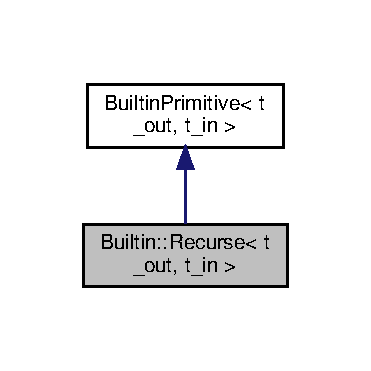
\includegraphics[width=178pt]{struct_builtin_1_1_recurse__inherit__graph}
\end{center}
\end{figure}


Collaboration diagram for Builtin\+:\+:Recurse$<$ t\+\_\+out, t\+\_\+in $>$\+:\nopagebreak
\begin{figure}[H]
\begin{center}
\leavevmode
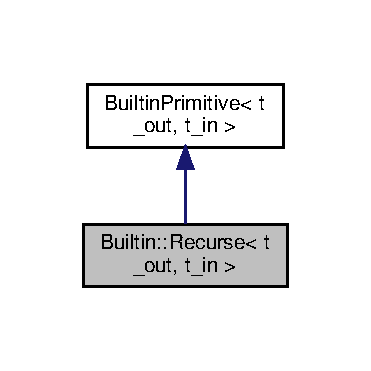
\includegraphics[width=178pt]{struct_builtin_1_1_recurse__coll__graph}
\end{center}
\end{figure}
\subsection*{Public Member Functions}
\begin{DoxyCompactItemize}
\item 
\hyperlink{struct_builtin_1_1_recurse_a1dc3290bbe19caff43bbf6814210033e}{Recurse} (std\+::string fmt, double \+\_\+p=1.\+0)
\end{DoxyCompactItemize}
\subsection*{Additional Inherited Members}


\subsection{Constructor \& Destructor Documentation}
\mbox{\Hypertarget{struct_builtin_1_1_recurse_a1dc3290bbe19caff43bbf6814210033e}\label{struct_builtin_1_1_recurse_a1dc3290bbe19caff43bbf6814210033e}} 
\index{Builtin\+::\+Recurse@{Builtin\+::\+Recurse}!Recurse@{Recurse}}
\index{Recurse@{Recurse}!Builtin\+::\+Recurse@{Builtin\+::\+Recurse}}
\subsubsection{\texorpdfstring{Recurse()}{Recurse()}}
{\footnotesize\ttfamily template$<$typename t\+\_\+out , typename t\+\_\+in $>$ \\
\hyperlink{struct_builtin_1_1_recurse}{Builtin\+::\+Recurse}$<$ t\+\_\+out, t\+\_\+in $>$\+::\hyperlink{struct_builtin_1_1_recurse}{Recurse} (\begin{DoxyParamCaption}\item[{std\+::string}]{fmt,  }\item[{double}]{\+\_\+p = {\ttfamily 1.0} }\end{DoxyParamCaption})\hspace{0.3cm}{\ttfamily [inline]}}



The documentation for this struct was generated from the following file\+:\begin{DoxyCompactItemize}
\item 
src/\+Virtual\+Machine/\hyperlink{_builtins_8h}{Builtins.\+h}\end{DoxyCompactItemize}

\hypertarget{class_fleet_1_1_statistics_1_1_reservoir_sample}{}\section{Fleet\+:\+:Statistics\+:\+:Reservoir\+Sample$<$ T $>$ Class Template Reference}
\label{class_fleet_1_1_statistics_1_1_reservoir_sample}\index{Fleet\+::\+Statistics\+::\+Reservoir\+Sample$<$ T $>$@{Fleet\+::\+Statistics\+::\+Reservoir\+Sample$<$ T $>$}}


{\ttfamily \#include $<$Reservoir\+Sample.\+h$>$}



Collaboration diagram for Fleet\+:\+:Statistics\+:\+:Reservoir\+Sample$<$ T $>$\+:
\nopagebreak
\begin{figure}[H]
\begin{center}
\leavevmode
\includegraphics[width=212pt]{class_fleet_1_1_statistics_1_1_reservoir_sample__coll__graph}
\end{center}
\end{figure}
\subsection*{Classes}
\begin{DoxyCompactItemize}
\item 
class \hyperlink{class_fleet_1_1_statistics_1_1_reservoir_sample_1_1_item}{Item}
\end{DoxyCompactItemize}
\subsection*{Public Member Functions}
\begin{DoxyCompactItemize}
\item 
\hyperlink{class_fleet_1_1_statistics_1_1_reservoir_sample_abb55ffa67b77f065407ec465c76c4eba}{Reservoir\+Sample} (size\+\_\+t n)
\item 
\hyperlink{class_fleet_1_1_statistics_1_1_reservoir_sample_abdbd4aeeed89ff5c6238fb64380faed0}{Reservoir\+Sample} ()
\item 
void \hyperlink{class_fleet_1_1_statistics_1_1_reservoir_sample_adabe7f40c91657950a67df7d20ace543}{set\+\_\+reservoir\+\_\+size} (const size\+\_\+t \hyperlink{class_fleet_1_1_statistics_1_1_reservoir_sample_a7cf0266d882988e2a61b857d123c8b58}{s}) const
\item 
size\+\_\+t \hyperlink{class_fleet_1_1_statistics_1_1_reservoir_sample_abdfad455c8b8da8cb2ab30d0f60053e0}{size} () const
\item 
void \hyperlink{class_fleet_1_1_statistics_1_1_reservoir_sample_a96005aae9818ace5255f2af95a631c66}{add} (T x)
\item 
void \hyperlink{class_fleet_1_1_statistics_1_1_reservoir_sample_ad6e4d50ef1acefce7f5d66013720c1ef}{operator$<$$<$} (T x)
\item 
std\+::vector$<$ T $>$ \hyperlink{class_fleet_1_1_statistics_1_1_reservoir_sample_a385d8640b316ff2e75f5da30948d8a35}{values} () const
\begin{DoxyCompactList}\small\item\em Get a multiset of values (ignoring the reservoir weights) \end{DoxyCompactList}\item 
T \hyperlink{class_fleet_1_1_statistics_1_1_reservoir_sample_a1b66a8f27512ebd6a48370621a43db87}{sample} () const
\item 
void \hyperlink{class_fleet_1_1_statistics_1_1_reservoir_sample_aadf45c574db6a4ab93da3df2b3f1df03}{clear} ()
\item 
\hyperlink{class_fleet_1_1_statistics_1_1_reservoir_sample_a0dde0cb8cfbb14a0bbf8db7f4bb316e9}{Reservoir\+Sample} (size\+\_\+t n, bool u=false)
\item 
\hyperlink{class_fleet_1_1_statistics_1_1_reservoir_sample_a39c8b405654eaca4c943263a485bc015}{Reservoir\+Sample} (bool u=false)
\item 
void \hyperlink{class_fleet_1_1_statistics_1_1_reservoir_sample_adabe7f40c91657950a67df7d20ace543}{set\+\_\+reservoir\+\_\+size} (const size\+\_\+t \hyperlink{class_fleet_1_1_statistics_1_1_reservoir_sample_a7cf0266d882988e2a61b857d123c8b58}{s}) const
\item 
size\+\_\+t \hyperlink{class_fleet_1_1_statistics_1_1_reservoir_sample_abdfad455c8b8da8cb2ab30d0f60053e0}{size} () const
\item 
T \hyperlink{class_fleet_1_1_statistics_1_1_reservoir_sample_af2d03d8d0e93ddedc61a43d1827ae48d}{max} ()
\item 
T \hyperlink{class_fleet_1_1_statistics_1_1_reservoir_sample_ab2f186b828351e164e1ed6e60c8c9be8}{min} ()
\item 
auto \hyperlink{class_fleet_1_1_statistics_1_1_reservoir_sample_af441a020b7a7244e9ca56c8d293fb59a}{begin} ()
\item 
auto \hyperlink{class_fleet_1_1_statistics_1_1_reservoir_sample_a4e3cf1195fcb255f2b0281d9307bfd16}{end} ()
\item 
double \hyperlink{class_fleet_1_1_statistics_1_1_reservoir_sample_aa802a85955db2941b99851f3b98e5252}{best\+\_\+posterior} () const
\item 
void \hyperlink{class_fleet_1_1_statistics_1_1_reservoir_sample_a374930296f502c957a925a5f7ba9087b}{add} (T x, double lw=0.\+0)
\item 
void \hyperlink{class_fleet_1_1_statistics_1_1_reservoir_sample_ad6e4d50ef1acefce7f5d66013720c1ef}{operator$<$$<$} (T x)
\item 
T \hyperlink{class_fleet_1_1_statistics_1_1_reservoir_sample_a1b66a8f27512ebd6a48370621a43db87}{sample} () const
\item 
void \hyperlink{class_fleet_1_1_statistics_1_1_reservoir_sample_aadf45c574db6a4ab93da3df2b3f1df03}{clear} ()
\end{DoxyCompactItemize}
\subsection*{Public Attributes}
\begin{DoxyCompactItemize}
\item 
\hyperlink{class_fleet_1_1_statistics_1_1_top_n}{Fleet\+::\+Statistics\+::\+TopN}$<$ \hyperlink{class_fleet_1_1_statistics_1_1_reservoir_sample_1_1_item}{Item} $>$ \hyperlink{class_fleet_1_1_statistics_1_1_reservoir_sample_ae14c8d6d8d5d6f1e3854710cf60b7716}{top}
\item 
unsigned long \hyperlink{class_fleet_1_1_statistics_1_1_reservoir_sample_a1e0c5104f173107e23900ff707df05ab}{N}
\item 
std\+::multiset$<$ \hyperlink{class_fleet_1_1_statistics_1_1_reservoir_sample_1_1_item}{Item} $>$ \hyperlink{class_fleet_1_1_statistics_1_1_reservoir_sample_a7cf0266d882988e2a61b857d123c8b58}{s}
\item 
std\+::multiset$<$ T $>$ \hyperlink{class_fleet_1_1_statistics_1_1_reservoir_sample_a9ffdb177a62651a2280099553124c433}{vals}
\item 
size\+\_\+t \hyperlink{class_fleet_1_1_statistics_1_1_reservoir_sample_a94ccb7246b63257eeee446ab4574387a}{reservoir\+\_\+size}
\item 
bool \hyperlink{class_fleet_1_1_statistics_1_1_reservoir_sample_ae3376d7008fd736ff141fa811aad4b65}{unique}
\end{DoxyCompactItemize}


\subsection{Detailed Description}
\subsubsection*{template$<$typename T$>$\newline
class Fleet\+::\+Statistics\+::\+Reservoir\+Sample$<$ T $>$}

\begin{DoxyAuthor}{Author}
piantado 
\end{DoxyAuthor}
\begin{DoxyDate}{Date}
29/01/20 
\end{DoxyDate}


\subsection{Constructor \& Destructor Documentation}
\mbox{\Hypertarget{class_fleet_1_1_statistics_1_1_reservoir_sample_abb55ffa67b77f065407ec465c76c4eba}\label{class_fleet_1_1_statistics_1_1_reservoir_sample_abb55ffa67b77f065407ec465c76c4eba}} 
\index{Fleet\+::\+Statistics\+::\+Reservoir\+Sample@{Fleet\+::\+Statistics\+::\+Reservoir\+Sample}!Reservoir\+Sample@{Reservoir\+Sample}}
\index{Reservoir\+Sample@{Reservoir\+Sample}!Fleet\+::\+Statistics\+::\+Reservoir\+Sample@{Fleet\+::\+Statistics\+::\+Reservoir\+Sample}}
\subsubsection{\texorpdfstring{Reservoir\+Sample()}{ReservoirSample()}\hspace{0.1cm}{\footnotesize\ttfamily [1/4]}}
{\footnotesize\ttfamily template$<$typename T$>$ \\
\hyperlink{class_fleet_1_1_statistics_1_1_reservoir_sample}{Fleet\+::\+Statistics\+::\+Reservoir\+Sample}$<$ T $>$\+::\hyperlink{class_fleet_1_1_statistics_1_1_reservoir_sample}{Reservoir\+Sample} (\begin{DoxyParamCaption}\item[{size\+\_\+t}]{n }\end{DoxyParamCaption})\hspace{0.3cm}{\ttfamily [inline]}}

\mbox{\Hypertarget{class_fleet_1_1_statistics_1_1_reservoir_sample_abdbd4aeeed89ff5c6238fb64380faed0}\label{class_fleet_1_1_statistics_1_1_reservoir_sample_abdbd4aeeed89ff5c6238fb64380faed0}} 
\index{Fleet\+::\+Statistics\+::\+Reservoir\+Sample@{Fleet\+::\+Statistics\+::\+Reservoir\+Sample}!Reservoir\+Sample@{Reservoir\+Sample}}
\index{Reservoir\+Sample@{Reservoir\+Sample}!Fleet\+::\+Statistics\+::\+Reservoir\+Sample@{Fleet\+::\+Statistics\+::\+Reservoir\+Sample}}
\subsubsection{\texorpdfstring{Reservoir\+Sample()}{ReservoirSample()}\hspace{0.1cm}{\footnotesize\ttfamily [2/4]}}
{\footnotesize\ttfamily template$<$typename T$>$ \\
\hyperlink{class_fleet_1_1_statistics_1_1_reservoir_sample}{Fleet\+::\+Statistics\+::\+Reservoir\+Sample}$<$ T $>$\+::\hyperlink{class_fleet_1_1_statistics_1_1_reservoir_sample}{Reservoir\+Sample} (\begin{DoxyParamCaption}{ }\end{DoxyParamCaption})\hspace{0.3cm}{\ttfamily [inline]}}

\mbox{\Hypertarget{class_fleet_1_1_statistics_1_1_reservoir_sample_a0dde0cb8cfbb14a0bbf8db7f4bb316e9}\label{class_fleet_1_1_statistics_1_1_reservoir_sample_a0dde0cb8cfbb14a0bbf8db7f4bb316e9}} 
\index{Fleet\+::\+Statistics\+::\+Reservoir\+Sample@{Fleet\+::\+Statistics\+::\+Reservoir\+Sample}!Reservoir\+Sample@{Reservoir\+Sample}}
\index{Reservoir\+Sample@{Reservoir\+Sample}!Fleet\+::\+Statistics\+::\+Reservoir\+Sample@{Fleet\+::\+Statistics\+::\+Reservoir\+Sample}}
\subsubsection{\texorpdfstring{Reservoir\+Sample()}{ReservoirSample()}\hspace{0.1cm}{\footnotesize\ttfamily [3/4]}}
{\footnotesize\ttfamily template$<$typename T$>$ \\
\hyperlink{class_fleet_1_1_statistics_1_1_reservoir_sample}{Fleet\+::\+Statistics\+::\+Reservoir\+Sample}$<$ T $>$\+::\hyperlink{class_fleet_1_1_statistics_1_1_reservoir_sample}{Reservoir\+Sample} (\begin{DoxyParamCaption}\item[{size\+\_\+t}]{n,  }\item[{bool}]{u = {\ttfamily false} }\end{DoxyParamCaption})\hspace{0.3cm}{\ttfamily [inline]}}

\mbox{\Hypertarget{class_fleet_1_1_statistics_1_1_reservoir_sample_a39c8b405654eaca4c943263a485bc015}\label{class_fleet_1_1_statistics_1_1_reservoir_sample_a39c8b405654eaca4c943263a485bc015}} 
\index{Fleet\+::\+Statistics\+::\+Reservoir\+Sample@{Fleet\+::\+Statistics\+::\+Reservoir\+Sample}!Reservoir\+Sample@{Reservoir\+Sample}}
\index{Reservoir\+Sample@{Reservoir\+Sample}!Fleet\+::\+Statistics\+::\+Reservoir\+Sample@{Fleet\+::\+Statistics\+::\+Reservoir\+Sample}}
\subsubsection{\texorpdfstring{Reservoir\+Sample()}{ReservoirSample()}\hspace{0.1cm}{\footnotesize\ttfamily [4/4]}}
{\footnotesize\ttfamily template$<$typename T$>$ \\
\hyperlink{class_fleet_1_1_statistics_1_1_reservoir_sample}{Fleet\+::\+Statistics\+::\+Reservoir\+Sample}$<$ T $>$\+::\hyperlink{class_fleet_1_1_statistics_1_1_reservoir_sample}{Reservoir\+Sample} (\begin{DoxyParamCaption}\item[{bool}]{u = {\ttfamily false} }\end{DoxyParamCaption})\hspace{0.3cm}{\ttfamily [inline]}}



\subsection{Member Function Documentation}
\mbox{\Hypertarget{class_fleet_1_1_statistics_1_1_reservoir_sample_a96005aae9818ace5255f2af95a631c66}\label{class_fleet_1_1_statistics_1_1_reservoir_sample_a96005aae9818ace5255f2af95a631c66}} 
\index{Fleet\+::\+Statistics\+::\+Reservoir\+Sample@{Fleet\+::\+Statistics\+::\+Reservoir\+Sample}!add@{add}}
\index{add@{add}!Fleet\+::\+Statistics\+::\+Reservoir\+Sample@{Fleet\+::\+Statistics\+::\+Reservoir\+Sample}}
\subsubsection{\texorpdfstring{add()}{add()}\hspace{0.1cm}{\footnotesize\ttfamily [1/2]}}
{\footnotesize\ttfamily template$<$typename T$>$ \\
void \hyperlink{class_fleet_1_1_statistics_1_1_reservoir_sample}{Fleet\+::\+Statistics\+::\+Reservoir\+Sample}$<$ T $>$\+::add (\begin{DoxyParamCaption}\item[{T}]{x }\end{DoxyParamCaption})\hspace{0.3cm}{\ttfamily [inline]}}

\mbox{\Hypertarget{class_fleet_1_1_statistics_1_1_reservoir_sample_a374930296f502c957a925a5f7ba9087b}\label{class_fleet_1_1_statistics_1_1_reservoir_sample_a374930296f502c957a925a5f7ba9087b}} 
\index{Fleet\+::\+Statistics\+::\+Reservoir\+Sample@{Fleet\+::\+Statistics\+::\+Reservoir\+Sample}!add@{add}}
\index{add@{add}!Fleet\+::\+Statistics\+::\+Reservoir\+Sample@{Fleet\+::\+Statistics\+::\+Reservoir\+Sample}}
\subsubsection{\texorpdfstring{add()}{add()}\hspace{0.1cm}{\footnotesize\ttfamily [2/2]}}
{\footnotesize\ttfamily template$<$typename T$>$ \\
void \hyperlink{class_fleet_1_1_statistics_1_1_reservoir_sample}{Fleet\+::\+Statistics\+::\+Reservoir\+Sample}$<$ T $>$\+::add (\begin{DoxyParamCaption}\item[{T}]{x,  }\item[{double}]{lw = {\ttfamily 0.0} }\end{DoxyParamCaption})\hspace{0.3cm}{\ttfamily [inline]}}

\mbox{\Hypertarget{class_fleet_1_1_statistics_1_1_reservoir_sample_af441a020b7a7244e9ca56c8d293fb59a}\label{class_fleet_1_1_statistics_1_1_reservoir_sample_af441a020b7a7244e9ca56c8d293fb59a}} 
\index{Fleet\+::\+Statistics\+::\+Reservoir\+Sample@{Fleet\+::\+Statistics\+::\+Reservoir\+Sample}!begin@{begin}}
\index{begin@{begin}!Fleet\+::\+Statistics\+::\+Reservoir\+Sample@{Fleet\+::\+Statistics\+::\+Reservoir\+Sample}}
\subsubsection{\texorpdfstring{begin()}{begin()}}
{\footnotesize\ttfamily template$<$typename T$>$ \\
auto \hyperlink{class_fleet_1_1_statistics_1_1_reservoir_sample}{Fleet\+::\+Statistics\+::\+Reservoir\+Sample}$<$ T $>$\+::begin (\begin{DoxyParamCaption}{ }\end{DoxyParamCaption})\hspace{0.3cm}{\ttfamily [inline]}}

\mbox{\Hypertarget{class_fleet_1_1_statistics_1_1_reservoir_sample_aa802a85955db2941b99851f3b98e5252}\label{class_fleet_1_1_statistics_1_1_reservoir_sample_aa802a85955db2941b99851f3b98e5252}} 
\index{Fleet\+::\+Statistics\+::\+Reservoir\+Sample@{Fleet\+::\+Statistics\+::\+Reservoir\+Sample}!best\+\_\+posterior@{best\+\_\+posterior}}
\index{best\+\_\+posterior@{best\+\_\+posterior}!Fleet\+::\+Statistics\+::\+Reservoir\+Sample@{Fleet\+::\+Statistics\+::\+Reservoir\+Sample}}
\subsubsection{\texorpdfstring{best\+\_\+posterior()}{best\_posterior()}}
{\footnotesize\ttfamily template$<$typename T$>$ \\
double \hyperlink{class_fleet_1_1_statistics_1_1_reservoir_sample}{Fleet\+::\+Statistics\+::\+Reservoir\+Sample}$<$ T $>$\+::best\+\_\+posterior (\begin{DoxyParamCaption}{ }\end{DoxyParamCaption}) const\hspace{0.3cm}{\ttfamily [inline]}}

What has the best posterior? \begin{DoxyReturn}{Returns}

\end{DoxyReturn}
\mbox{\Hypertarget{class_fleet_1_1_statistics_1_1_reservoir_sample_aadf45c574db6a4ab93da3df2b3f1df03}\label{class_fleet_1_1_statistics_1_1_reservoir_sample_aadf45c574db6a4ab93da3df2b3f1df03}} 
\index{Fleet\+::\+Statistics\+::\+Reservoir\+Sample@{Fleet\+::\+Statistics\+::\+Reservoir\+Sample}!clear@{clear}}
\index{clear@{clear}!Fleet\+::\+Statistics\+::\+Reservoir\+Sample@{Fleet\+::\+Statistics\+::\+Reservoir\+Sample}}
\subsubsection{\texorpdfstring{clear()}{clear()}\hspace{0.1cm}{\footnotesize\ttfamily [1/2]}}
{\footnotesize\ttfamily template$<$typename T$>$ \\
void \hyperlink{class_fleet_1_1_statistics_1_1_reservoir_sample}{Fleet\+::\+Statistics\+::\+Reservoir\+Sample}$<$ T $>$\+::clear (\begin{DoxyParamCaption}{ }\end{DoxyParamCaption})\hspace{0.3cm}{\ttfamily [inline]}}

\mbox{\Hypertarget{class_fleet_1_1_statistics_1_1_reservoir_sample_aadf45c574db6a4ab93da3df2b3f1df03}\label{class_fleet_1_1_statistics_1_1_reservoir_sample_aadf45c574db6a4ab93da3df2b3f1df03}} 
\index{Fleet\+::\+Statistics\+::\+Reservoir\+Sample@{Fleet\+::\+Statistics\+::\+Reservoir\+Sample}!clear@{clear}}
\index{clear@{clear}!Fleet\+::\+Statistics\+::\+Reservoir\+Sample@{Fleet\+::\+Statistics\+::\+Reservoir\+Sample}}
\subsubsection{\texorpdfstring{clear()}{clear()}\hspace{0.1cm}{\footnotesize\ttfamily [2/2]}}
{\footnotesize\ttfamily template$<$typename T$>$ \\
void \hyperlink{class_fleet_1_1_statistics_1_1_reservoir_sample}{Fleet\+::\+Statistics\+::\+Reservoir\+Sample}$<$ T $>$\+::clear (\begin{DoxyParamCaption}{ }\end{DoxyParamCaption})\hspace{0.3cm}{\ttfamily [inline]}}

\mbox{\Hypertarget{class_fleet_1_1_statistics_1_1_reservoir_sample_a4e3cf1195fcb255f2b0281d9307bfd16}\label{class_fleet_1_1_statistics_1_1_reservoir_sample_a4e3cf1195fcb255f2b0281d9307bfd16}} 
\index{Fleet\+::\+Statistics\+::\+Reservoir\+Sample@{Fleet\+::\+Statistics\+::\+Reservoir\+Sample}!end@{end}}
\index{end@{end}!Fleet\+::\+Statistics\+::\+Reservoir\+Sample@{Fleet\+::\+Statistics\+::\+Reservoir\+Sample}}
\subsubsection{\texorpdfstring{end()}{end()}}
{\footnotesize\ttfamily template$<$typename T$>$ \\
auto \hyperlink{class_fleet_1_1_statistics_1_1_reservoir_sample}{Fleet\+::\+Statistics\+::\+Reservoir\+Sample}$<$ T $>$\+::end (\begin{DoxyParamCaption}{ }\end{DoxyParamCaption})\hspace{0.3cm}{\ttfamily [inline]}}

\mbox{\Hypertarget{class_fleet_1_1_statistics_1_1_reservoir_sample_af2d03d8d0e93ddedc61a43d1827ae48d}\label{class_fleet_1_1_statistics_1_1_reservoir_sample_af2d03d8d0e93ddedc61a43d1827ae48d}} 
\index{Fleet\+::\+Statistics\+::\+Reservoir\+Sample@{Fleet\+::\+Statistics\+::\+Reservoir\+Sample}!max@{max}}
\index{max@{max}!Fleet\+::\+Statistics\+::\+Reservoir\+Sample@{Fleet\+::\+Statistics\+::\+Reservoir\+Sample}}
\subsubsection{\texorpdfstring{max()}{max()}}
{\footnotesize\ttfamily template$<$typename T$>$ \\
T \hyperlink{class_fleet_1_1_statistics_1_1_reservoir_sample}{Fleet\+::\+Statistics\+::\+Reservoir\+Sample}$<$ T $>$\+::max (\begin{DoxyParamCaption}{ }\end{DoxyParamCaption})\hspace{0.3cm}{\ttfamily [inline]}}

\mbox{\Hypertarget{class_fleet_1_1_statistics_1_1_reservoir_sample_ab2f186b828351e164e1ed6e60c8c9be8}\label{class_fleet_1_1_statistics_1_1_reservoir_sample_ab2f186b828351e164e1ed6e60c8c9be8}} 
\index{Fleet\+::\+Statistics\+::\+Reservoir\+Sample@{Fleet\+::\+Statistics\+::\+Reservoir\+Sample}!min@{min}}
\index{min@{min}!Fleet\+::\+Statistics\+::\+Reservoir\+Sample@{Fleet\+::\+Statistics\+::\+Reservoir\+Sample}}
\subsubsection{\texorpdfstring{min()}{min()}}
{\footnotesize\ttfamily template$<$typename T$>$ \\
T \hyperlink{class_fleet_1_1_statistics_1_1_reservoir_sample}{Fleet\+::\+Statistics\+::\+Reservoir\+Sample}$<$ T $>$\+::min (\begin{DoxyParamCaption}{ }\end{DoxyParamCaption})\hspace{0.3cm}{\ttfamily [inline]}}

\mbox{\Hypertarget{class_fleet_1_1_statistics_1_1_reservoir_sample_ad6e4d50ef1acefce7f5d66013720c1ef}\label{class_fleet_1_1_statistics_1_1_reservoir_sample_ad6e4d50ef1acefce7f5d66013720c1ef}} 
\index{Fleet\+::\+Statistics\+::\+Reservoir\+Sample@{Fleet\+::\+Statistics\+::\+Reservoir\+Sample}!operator$<$$<$@{operator$<$$<$}}
\index{operator$<$$<$@{operator$<$$<$}!Fleet\+::\+Statistics\+::\+Reservoir\+Sample@{Fleet\+::\+Statistics\+::\+Reservoir\+Sample}}
\subsubsection{\texorpdfstring{operator$<$$<$()}{operator<<()}\hspace{0.1cm}{\footnotesize\ttfamily [1/2]}}
{\footnotesize\ttfamily template$<$typename T$>$ \\
void \hyperlink{class_fleet_1_1_statistics_1_1_reservoir_sample}{Fleet\+::\+Statistics\+::\+Reservoir\+Sample}$<$ T $>$\+::operator$<$$<$ (\begin{DoxyParamCaption}\item[{T}]{x }\end{DoxyParamCaption})\hspace{0.3cm}{\ttfamily [inline]}}

\mbox{\Hypertarget{class_fleet_1_1_statistics_1_1_reservoir_sample_ad6e4d50ef1acefce7f5d66013720c1ef}\label{class_fleet_1_1_statistics_1_1_reservoir_sample_ad6e4d50ef1acefce7f5d66013720c1ef}} 
\index{Fleet\+::\+Statistics\+::\+Reservoir\+Sample@{Fleet\+::\+Statistics\+::\+Reservoir\+Sample}!operator$<$$<$@{operator$<$$<$}}
\index{operator$<$$<$@{operator$<$$<$}!Fleet\+::\+Statistics\+::\+Reservoir\+Sample@{Fleet\+::\+Statistics\+::\+Reservoir\+Sample}}
\subsubsection{\texorpdfstring{operator$<$$<$()}{operator<<()}\hspace{0.1cm}{\footnotesize\ttfamily [2/2]}}
{\footnotesize\ttfamily template$<$typename T$>$ \\
void \hyperlink{class_fleet_1_1_statistics_1_1_reservoir_sample}{Fleet\+::\+Statistics\+::\+Reservoir\+Sample}$<$ T $>$\+::operator$<$$<$ (\begin{DoxyParamCaption}\item[{T}]{x }\end{DoxyParamCaption})\hspace{0.3cm}{\ttfamily [inline]}}

\mbox{\Hypertarget{class_fleet_1_1_statistics_1_1_reservoir_sample_a1b66a8f27512ebd6a48370621a43db87}\label{class_fleet_1_1_statistics_1_1_reservoir_sample_a1b66a8f27512ebd6a48370621a43db87}} 
\index{Fleet\+::\+Statistics\+::\+Reservoir\+Sample@{Fleet\+::\+Statistics\+::\+Reservoir\+Sample}!sample@{sample}}
\index{sample@{sample}!Fleet\+::\+Statistics\+::\+Reservoir\+Sample@{Fleet\+::\+Statistics\+::\+Reservoir\+Sample}}
\subsubsection{\texorpdfstring{sample()}{sample()}\hspace{0.1cm}{\footnotesize\ttfamily [1/2]}}
{\footnotesize\ttfamily template$<$typename T$>$ \\
T \hyperlink{class_fleet_1_1_statistics_1_1_reservoir_sample}{Fleet\+::\+Statistics\+::\+Reservoir\+Sample}$<$ T $>$\+::sample (\begin{DoxyParamCaption}{ }\end{DoxyParamCaption}) const\hspace{0.3cm}{\ttfamily [inline]}}

Return a sample from my vals \begin{DoxyReturn}{Returns}

\end{DoxyReturn}
\mbox{\Hypertarget{class_fleet_1_1_statistics_1_1_reservoir_sample_a1b66a8f27512ebd6a48370621a43db87}\label{class_fleet_1_1_statistics_1_1_reservoir_sample_a1b66a8f27512ebd6a48370621a43db87}} 
\index{Fleet\+::\+Statistics\+::\+Reservoir\+Sample@{Fleet\+::\+Statistics\+::\+Reservoir\+Sample}!sample@{sample}}
\index{sample@{sample}!Fleet\+::\+Statistics\+::\+Reservoir\+Sample@{Fleet\+::\+Statistics\+::\+Reservoir\+Sample}}
\subsubsection{\texorpdfstring{sample()}{sample()}\hspace{0.1cm}{\footnotesize\ttfamily [2/2]}}
{\footnotesize\ttfamily template$<$typename T$>$ \\
T \hyperlink{class_fleet_1_1_statistics_1_1_reservoir_sample}{Fleet\+::\+Statistics\+::\+Reservoir\+Sample}$<$ T $>$\+::sample (\begin{DoxyParamCaption}{ }\end{DoxyParamCaption}) const\hspace{0.3cm}{\ttfamily [inline]}}

Return a sample from my vals (e.\+g. a sample of the samples I happen to have saved) \begin{DoxyReturn}{Returns}

\end{DoxyReturn}
\mbox{\Hypertarget{class_fleet_1_1_statistics_1_1_reservoir_sample_adabe7f40c91657950a67df7d20ace543}\label{class_fleet_1_1_statistics_1_1_reservoir_sample_adabe7f40c91657950a67df7d20ace543}} 
\index{Fleet\+::\+Statistics\+::\+Reservoir\+Sample@{Fleet\+::\+Statistics\+::\+Reservoir\+Sample}!set\+\_\+reservoir\+\_\+size@{set\+\_\+reservoir\+\_\+size}}
\index{set\+\_\+reservoir\+\_\+size@{set\+\_\+reservoir\+\_\+size}!Fleet\+::\+Statistics\+::\+Reservoir\+Sample@{Fleet\+::\+Statistics\+::\+Reservoir\+Sample}}
\subsubsection{\texorpdfstring{set\+\_\+reservoir\+\_\+size()}{set\_reservoir\_size()}\hspace{0.1cm}{\footnotesize\ttfamily [1/2]}}
{\footnotesize\ttfamily template$<$typename T$>$ \\
void \hyperlink{class_fleet_1_1_statistics_1_1_reservoir_sample}{Fleet\+::\+Statistics\+::\+Reservoir\+Sample}$<$ T $>$\+::set\+\_\+reservoir\+\_\+size (\begin{DoxyParamCaption}\item[{const size\+\_\+t}]{s }\end{DoxyParamCaption}) const\hspace{0.3cm}{\ttfamily [inline]}}

How big should the reservoir size be? 
\begin{DoxyParams}{Parameters}
{\em s} & \\
\hline
\end{DoxyParams}
\mbox{\Hypertarget{class_fleet_1_1_statistics_1_1_reservoir_sample_adabe7f40c91657950a67df7d20ace543}\label{class_fleet_1_1_statistics_1_1_reservoir_sample_adabe7f40c91657950a67df7d20ace543}} 
\index{Fleet\+::\+Statistics\+::\+Reservoir\+Sample@{Fleet\+::\+Statistics\+::\+Reservoir\+Sample}!set\+\_\+reservoir\+\_\+size@{set\+\_\+reservoir\+\_\+size}}
\index{set\+\_\+reservoir\+\_\+size@{set\+\_\+reservoir\+\_\+size}!Fleet\+::\+Statistics\+::\+Reservoir\+Sample@{Fleet\+::\+Statistics\+::\+Reservoir\+Sample}}
\subsubsection{\texorpdfstring{set\+\_\+reservoir\+\_\+size()}{set\_reservoir\_size()}\hspace{0.1cm}{\footnotesize\ttfamily [2/2]}}
{\footnotesize\ttfamily template$<$typename T$>$ \\
void \hyperlink{class_fleet_1_1_statistics_1_1_reservoir_sample}{Fleet\+::\+Statistics\+::\+Reservoir\+Sample}$<$ T $>$\+::set\+\_\+reservoir\+\_\+size (\begin{DoxyParamCaption}\item[{const size\+\_\+t}]{s }\end{DoxyParamCaption}) const\hspace{0.3cm}{\ttfamily [inline]}}

How big should the reservoir size be? 
\begin{DoxyParams}{Parameters}
{\em s} & \\
\hline
\end{DoxyParams}
\mbox{\Hypertarget{class_fleet_1_1_statistics_1_1_reservoir_sample_abdfad455c8b8da8cb2ab30d0f60053e0}\label{class_fleet_1_1_statistics_1_1_reservoir_sample_abdfad455c8b8da8cb2ab30d0f60053e0}} 
\index{Fleet\+::\+Statistics\+::\+Reservoir\+Sample@{Fleet\+::\+Statistics\+::\+Reservoir\+Sample}!size@{size}}
\index{size@{size}!Fleet\+::\+Statistics\+::\+Reservoir\+Sample@{Fleet\+::\+Statistics\+::\+Reservoir\+Sample}}
\subsubsection{\texorpdfstring{size()}{size()}\hspace{0.1cm}{\footnotesize\ttfamily [1/2]}}
{\footnotesize\ttfamily template$<$typename T$>$ \\
size\+\_\+t \hyperlink{class_fleet_1_1_statistics_1_1_reservoir_sample}{Fleet\+::\+Statistics\+::\+Reservoir\+Sample}$<$ T $>$\+::size (\begin{DoxyParamCaption}{ }\end{DoxyParamCaption}) const\hspace{0.3cm}{\ttfamily [inline]}}

How many elements are currently stored? \begin{DoxyReturn}{Returns}

\end{DoxyReturn}
\mbox{\Hypertarget{class_fleet_1_1_statistics_1_1_reservoir_sample_abdfad455c8b8da8cb2ab30d0f60053e0}\label{class_fleet_1_1_statistics_1_1_reservoir_sample_abdfad455c8b8da8cb2ab30d0f60053e0}} 
\index{Fleet\+::\+Statistics\+::\+Reservoir\+Sample@{Fleet\+::\+Statistics\+::\+Reservoir\+Sample}!size@{size}}
\index{size@{size}!Fleet\+::\+Statistics\+::\+Reservoir\+Sample@{Fleet\+::\+Statistics\+::\+Reservoir\+Sample}}
\subsubsection{\texorpdfstring{size()}{size()}\hspace{0.1cm}{\footnotesize\ttfamily [2/2]}}
{\footnotesize\ttfamily template$<$typename T$>$ \\
size\+\_\+t \hyperlink{class_fleet_1_1_statistics_1_1_reservoir_sample}{Fleet\+::\+Statistics\+::\+Reservoir\+Sample}$<$ T $>$\+::size (\begin{DoxyParamCaption}{ }\end{DoxyParamCaption}) const\hspace{0.3cm}{\ttfamily [inline]}}

How many elements are currently stored? \begin{DoxyReturn}{Returns}

\end{DoxyReturn}
\mbox{\Hypertarget{class_fleet_1_1_statistics_1_1_reservoir_sample_a385d8640b316ff2e75f5da30948d8a35}\label{class_fleet_1_1_statistics_1_1_reservoir_sample_a385d8640b316ff2e75f5da30948d8a35}} 
\index{Fleet\+::\+Statistics\+::\+Reservoir\+Sample@{Fleet\+::\+Statistics\+::\+Reservoir\+Sample}!values@{values}}
\index{values@{values}!Fleet\+::\+Statistics\+::\+Reservoir\+Sample@{Fleet\+::\+Statistics\+::\+Reservoir\+Sample}}
\subsubsection{\texorpdfstring{values()}{values()}}
{\footnotesize\ttfamily template$<$typename T$>$ \\
std\+::vector$<$T$>$ \hyperlink{class_fleet_1_1_statistics_1_1_reservoir_sample}{Fleet\+::\+Statistics\+::\+Reservoir\+Sample}$<$ T $>$\+::values (\begin{DoxyParamCaption}{ }\end{DoxyParamCaption}) const\hspace{0.3cm}{\ttfamily [inline]}}



Get a multiset of values (ignoring the reservoir weights) 

\begin{DoxyReturn}{Returns}

\end{DoxyReturn}


\subsection{Member Data Documentation}
\mbox{\Hypertarget{class_fleet_1_1_statistics_1_1_reservoir_sample_a1e0c5104f173107e23900ff707df05ab}\label{class_fleet_1_1_statistics_1_1_reservoir_sample_a1e0c5104f173107e23900ff707df05ab}} 
\index{Fleet\+::\+Statistics\+::\+Reservoir\+Sample@{Fleet\+::\+Statistics\+::\+Reservoir\+Sample}!N@{N}}
\index{N@{N}!Fleet\+::\+Statistics\+::\+Reservoir\+Sample@{Fleet\+::\+Statistics\+::\+Reservoir\+Sample}}
\subsubsection{\texorpdfstring{N}{N}}
{\footnotesize\ttfamily template$<$typename T$>$ \\
unsigned long \hyperlink{class_fleet_1_1_statistics_1_1_reservoir_sample}{Fleet\+::\+Statistics\+::\+Reservoir\+Sample}$<$ T $>$\+::N}

\mbox{\Hypertarget{class_fleet_1_1_statistics_1_1_reservoir_sample_a94ccb7246b63257eeee446ab4574387a}\label{class_fleet_1_1_statistics_1_1_reservoir_sample_a94ccb7246b63257eeee446ab4574387a}} 
\index{Fleet\+::\+Statistics\+::\+Reservoir\+Sample@{Fleet\+::\+Statistics\+::\+Reservoir\+Sample}!reservoir\+\_\+size@{reservoir\+\_\+size}}
\index{reservoir\+\_\+size@{reservoir\+\_\+size}!Fleet\+::\+Statistics\+::\+Reservoir\+Sample@{Fleet\+::\+Statistics\+::\+Reservoir\+Sample}}
\subsubsection{\texorpdfstring{reservoir\+\_\+size}{reservoir\_size}}
{\footnotesize\ttfamily template$<$typename T$>$ \\
size\+\_\+t \hyperlink{class_fleet_1_1_statistics_1_1_reservoir_sample}{Fleet\+::\+Statistics\+::\+Reservoir\+Sample}$<$ T $>$\+::reservoir\+\_\+size}

\mbox{\Hypertarget{class_fleet_1_1_statistics_1_1_reservoir_sample_a7cf0266d882988e2a61b857d123c8b58}\label{class_fleet_1_1_statistics_1_1_reservoir_sample_a7cf0266d882988e2a61b857d123c8b58}} 
\index{Fleet\+::\+Statistics\+::\+Reservoir\+Sample@{Fleet\+::\+Statistics\+::\+Reservoir\+Sample}!s@{s}}
\index{s@{s}!Fleet\+::\+Statistics\+::\+Reservoir\+Sample@{Fleet\+::\+Statistics\+::\+Reservoir\+Sample}}
\subsubsection{\texorpdfstring{s}{s}}
{\footnotesize\ttfamily template$<$typename T$>$ \\
std\+::multiset$<$\hyperlink{class_fleet_1_1_statistics_1_1_reservoir_sample_1_1_item}{Item}$>$ \hyperlink{class_fleet_1_1_statistics_1_1_reservoir_sample}{Fleet\+::\+Statistics\+::\+Reservoir\+Sample}$<$ T $>$\+::s}

\mbox{\Hypertarget{class_fleet_1_1_statistics_1_1_reservoir_sample_ae14c8d6d8d5d6f1e3854710cf60b7716}\label{class_fleet_1_1_statistics_1_1_reservoir_sample_ae14c8d6d8d5d6f1e3854710cf60b7716}} 
\index{Fleet\+::\+Statistics\+::\+Reservoir\+Sample@{Fleet\+::\+Statistics\+::\+Reservoir\+Sample}!top@{top}}
\index{top@{top}!Fleet\+::\+Statistics\+::\+Reservoir\+Sample@{Fleet\+::\+Statistics\+::\+Reservoir\+Sample}}
\subsubsection{\texorpdfstring{top}{top}}
{\footnotesize\ttfamily template$<$typename T$>$ \\
\hyperlink{class_fleet_1_1_statistics_1_1_top_n}{Fleet\+::\+Statistics\+::\+TopN}$<$\hyperlink{class_fleet_1_1_statistics_1_1_reservoir_sample_1_1_item}{Item}$>$ \hyperlink{class_fleet_1_1_statistics_1_1_reservoir_sample}{Fleet\+::\+Statistics\+::\+Reservoir\+Sample}$<$ T $>$\+::top}

\mbox{\Hypertarget{class_fleet_1_1_statistics_1_1_reservoir_sample_ae3376d7008fd736ff141fa811aad4b65}\label{class_fleet_1_1_statistics_1_1_reservoir_sample_ae3376d7008fd736ff141fa811aad4b65}} 
\index{Fleet\+::\+Statistics\+::\+Reservoir\+Sample@{Fleet\+::\+Statistics\+::\+Reservoir\+Sample}!unique@{unique}}
\index{unique@{unique}!Fleet\+::\+Statistics\+::\+Reservoir\+Sample@{Fleet\+::\+Statistics\+::\+Reservoir\+Sample}}
\subsubsection{\texorpdfstring{unique}{unique}}
{\footnotesize\ttfamily template$<$typename T$>$ \\
bool \hyperlink{class_fleet_1_1_statistics_1_1_reservoir_sample}{Fleet\+::\+Statistics\+::\+Reservoir\+Sample}$<$ T $>$\+::unique}

\mbox{\Hypertarget{class_fleet_1_1_statistics_1_1_reservoir_sample_a9ffdb177a62651a2280099553124c433}\label{class_fleet_1_1_statistics_1_1_reservoir_sample_a9ffdb177a62651a2280099553124c433}} 
\index{Fleet\+::\+Statistics\+::\+Reservoir\+Sample@{Fleet\+::\+Statistics\+::\+Reservoir\+Sample}!vals@{vals}}
\index{vals@{vals}!Fleet\+::\+Statistics\+::\+Reservoir\+Sample@{Fleet\+::\+Statistics\+::\+Reservoir\+Sample}}
\subsubsection{\texorpdfstring{vals}{vals}}
{\footnotesize\ttfamily template$<$typename T$>$ \\
std\+::multiset$<$T$>$ \hyperlink{class_fleet_1_1_statistics_1_1_reservoir_sample}{Fleet\+::\+Statistics\+::\+Reservoir\+Sample}$<$ T $>$\+::vals}



The documentation for this class was generated from the following files\+:\begin{DoxyCompactItemize}
\item 
src/\+Statistics/\hyperlink{_reservoir_sample_8h}{Reservoir\+Sample.\+h}\item 
src/\+Statistics/\hyperlink{_reservoir_sample__old_8h}{Reservoir\+Sample\+\_\+old.\+h}\end{DoxyCompactItemize}

\hypertarget{class_rule}{}\section{Rule Class Reference}
\label{class_rule}\index{Rule@{Rule}}


{\ttfamily \#include $<$Rule.\+h$>$}



Collaboration diagram for Rule\+:\nopagebreak
\begin{figure}[H]
\begin{center}
\leavevmode
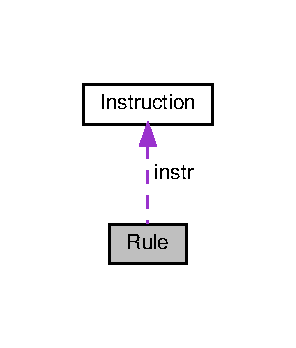
\includegraphics[width=142pt]{class_rule__coll__graph}
\end{center}
\end{figure}
\subsection*{Public Member Functions}
\begin{DoxyCompactItemize}
\item 
{\footnotesize template$<$typename O\+PT $>$ }\\\hyperlink{class_rule_a1e65fa1bce404b1513038a9dd4ffcb9f}{Rule} (const nonterminal\+\_\+t rt, const O\+PT o, const std\+::string fmt, std\+::initializer\+\_\+list$<$ nonterminal\+\_\+t $>$ c, double \+\_\+p, const int arg=0)
\item 
bool \hyperlink{class_rule_a706819fbede2c5a1b0b59f1d28cae30b}{operator$<$} (const \hyperlink{class_rule}{Rule} \&r) const
\item 
bool \hyperlink{class_rule_a183fafc8a6b43515436a1de8f63ec98d}{operator==} (const \hyperlink{class_rule}{Rule} \&r) const
\item 
size\+\_\+t \hyperlink{class_rule_a62e4d931266a65d4aad9ca3c058d7e25}{get\+\_\+hash} () const
\item 
bool \hyperlink{class_rule_a9d557e302f94bd85f5505733e8856f97}{is\+\_\+terminal} () const
\item 
nonterminal\+\_\+t \hyperlink{class_rule_a97db8e22bb8445b92779eb165bb29ae5}{type} (size\+\_\+t i) const
\item 
std\+::string \hyperlink{class_rule_a4a75588d7821c1bcf087ec6ebf82bd0f}{string} ()
\end{DoxyCompactItemize}
\subsection*{Public Attributes}
\begin{DoxyCompactItemize}
\item 
nonterminal\+\_\+t \hyperlink{class_rule_a980385e76137909454bd6a585bd2e138}{nt}
\item 
\hyperlink{class_instruction}{Instruction} \hyperlink{class_rule_a367e578f5e1427ef04d1d77477565c67}{instr}
\item 
std\+::string \hyperlink{class_rule_aa48c15aaaf5242afea0439607f2a2177}{format}
\item 
size\+\_\+t \hyperlink{class_rule_a0a2a742af39b60831ad1ac5eb5ba7498}{N}
\item 
double \hyperlink{class_rule_acd7e4d41d59dec76f60ca16238ab391a}{p}
\end{DoxyCompactItemize}
\subsection*{Protected Attributes}
\begin{DoxyCompactItemize}
\item 
nonterminal\+\_\+t \hyperlink{class_rule_a2d5160625d3d15f60690c4323522a33e}{child\+\_\+types} \mbox{[}Fleet\+::\+M\+A\+X\+\_\+\+C\+H\+I\+L\+D\+\_\+\+S\+I\+ZE\mbox{]}
\item 
std\+::size\+\_\+t \hyperlink{class_rule_af2d873c97e2de425f14a5a980dbcc104}{my\+\_\+hash}
\end{DoxyCompactItemize}


\subsection{Constructor \& Destructor Documentation}
\mbox{\Hypertarget{class_rule_a1e65fa1bce404b1513038a9dd4ffcb9f}\label{class_rule_a1e65fa1bce404b1513038a9dd4ffcb9f}} 
\index{Rule@{Rule}!Rule@{Rule}}
\index{Rule@{Rule}!Rule@{Rule}}
\subsubsection{\texorpdfstring{Rule()}{Rule()}}
{\footnotesize\ttfamily template$<$typename O\+PT $>$ \\
Rule\+::\+Rule (\begin{DoxyParamCaption}\item[{const nonterminal\+\_\+t}]{rt,  }\item[{const O\+PT}]{o,  }\item[{const std\+::string}]{fmt,  }\item[{std\+::initializer\+\_\+list$<$ nonterminal\+\_\+t $>$}]{c,  }\item[{double}]{\+\_\+p,  }\item[{const int}]{arg = {\ttfamily 0} }\end{DoxyParamCaption})\hspace{0.3cm}{\ttfamily [inline]}}



\subsection{Member Function Documentation}
\mbox{\Hypertarget{class_rule_a62e4d931266a65d4aad9ca3c058d7e25}\label{class_rule_a62e4d931266a65d4aad9ca3c058d7e25}} 
\index{Rule@{Rule}!get\+\_\+hash@{get\+\_\+hash}}
\index{get\+\_\+hash@{get\+\_\+hash}!Rule@{Rule}}
\subsubsection{\texorpdfstring{get\+\_\+hash()}{get\_hash()}}
{\footnotesize\ttfamily size\+\_\+t Rule\+::get\+\_\+hash (\begin{DoxyParamCaption}{ }\end{DoxyParamCaption}) const\hspace{0.3cm}{\ttfamily [inline]}}

\mbox{\Hypertarget{class_rule_a9d557e302f94bd85f5505733e8856f97}\label{class_rule_a9d557e302f94bd85f5505733e8856f97}} 
\index{Rule@{Rule}!is\+\_\+terminal@{is\+\_\+terminal}}
\index{is\+\_\+terminal@{is\+\_\+terminal}!Rule@{Rule}}
\subsubsection{\texorpdfstring{is\+\_\+terminal()}{is\_terminal()}}
{\footnotesize\ttfamily bool Rule\+::is\+\_\+terminal (\begin{DoxyParamCaption}{ }\end{DoxyParamCaption}) const\hspace{0.3cm}{\ttfamily [inline]}}

A terminal rule has no children. \begin{DoxyReturn}{Returns}

\end{DoxyReturn}
\mbox{\Hypertarget{class_rule_a706819fbede2c5a1b0b59f1d28cae30b}\label{class_rule_a706819fbede2c5a1b0b59f1d28cae30b}} 
\index{Rule@{Rule}!operator$<$@{operator$<$}}
\index{operator$<$@{operator$<$}!Rule@{Rule}}
\subsubsection{\texorpdfstring{operator$<$()}{operator<()}}
{\footnotesize\ttfamily bool Rule\+::operator$<$ (\begin{DoxyParamCaption}\item[{const \hyperlink{class_rule}{Rule} \&}]{r }\end{DoxyParamCaption}) const\hspace{0.3cm}{\ttfamily [inline]}}

We sort rules so that they can be stored in arrays in a standard order. For enumeration, it\textquotesingle{}s actually important that we sort them with the terminals first. So we sort first by terminals and then by probability (higher first). 
\begin{DoxyParams}{Parameters}
{\em r} & \\
\hline
\end{DoxyParams}
\begin{DoxyReturn}{Returns}

\end{DoxyReturn}
\mbox{\Hypertarget{class_rule_a183fafc8a6b43515436a1de8f63ec98d}\label{class_rule_a183fafc8a6b43515436a1de8f63ec98d}} 
\index{Rule@{Rule}!operator==@{operator==}}
\index{operator==@{operator==}!Rule@{Rule}}
\subsubsection{\texorpdfstring{operator==()}{operator==()}}
{\footnotesize\ttfamily bool Rule\+::operator== (\begin{DoxyParamCaption}\item[{const \hyperlink{class_rule}{Rule} \&}]{r }\end{DoxyParamCaption}) const\hspace{0.3cm}{\ttfamily [inline]}}

Two rules are equal if they have the same instructions, nonterminal, format, children, and children types 
\begin{DoxyParams}{Parameters}
{\em r} & \\
\hline
\end{DoxyParams}
\begin{DoxyReturn}{Returns}

\end{DoxyReturn}
\mbox{\Hypertarget{class_rule_a4a75588d7821c1bcf087ec6ebf82bd0f}\label{class_rule_a4a75588d7821c1bcf087ec6ebf82bd0f}} 
\index{Rule@{Rule}!string@{string}}
\index{string@{string}!Rule@{Rule}}
\subsubsection{\texorpdfstring{string()}{string()}}
{\footnotesize\ttfamily std\+::string Rule\+::string (\begin{DoxyParamCaption}{ }\end{DoxyParamCaption})\hspace{0.3cm}{\ttfamily [inline]}}

\mbox{\Hypertarget{class_rule_a97db8e22bb8445b92779eb165bb29ae5}\label{class_rule_a97db8e22bb8445b92779eb165bb29ae5}} 
\index{Rule@{Rule}!type@{type}}
\index{type@{type}!Rule@{Rule}}
\subsubsection{\texorpdfstring{type()}{type()}}
{\footnotesize\ttfamily nonterminal\+\_\+t Rule\+::type (\begin{DoxyParamCaption}\item[{size\+\_\+t}]{i }\end{DoxyParamCaption}) const\hspace{0.3cm}{\ttfamily [inline]}}

What type is my i\textquotesingle{}th child? 
\begin{DoxyParams}{Parameters}
{\em i} & \\
\hline
\end{DoxyParams}
\begin{DoxyReturn}{Returns}

\end{DoxyReturn}


\subsection{Member Data Documentation}
\mbox{\Hypertarget{class_rule_a2d5160625d3d15f60690c4323522a33e}\label{class_rule_a2d5160625d3d15f60690c4323522a33e}} 
\index{Rule@{Rule}!child\+\_\+types@{child\+\_\+types}}
\index{child\+\_\+types@{child\+\_\+types}!Rule@{Rule}}
\subsubsection{\texorpdfstring{child\+\_\+types}{child\_types}}
{\footnotesize\ttfamily nonterminal\+\_\+t Rule\+::child\+\_\+types\mbox{[}Fleet\+::\+M\+A\+X\+\_\+\+C\+H\+I\+L\+D\+\_\+\+S\+I\+ZE\mbox{]}\hspace{0.3cm}{\ttfamily [protected]}}

\mbox{\Hypertarget{class_rule_aa48c15aaaf5242afea0439607f2a2177}\label{class_rule_aa48c15aaaf5242afea0439607f2a2177}} 
\index{Rule@{Rule}!format@{format}}
\index{format@{format}!Rule@{Rule}}
\subsubsection{\texorpdfstring{format}{format}}
{\footnotesize\ttfamily std\+::string Rule\+::format}

\mbox{\Hypertarget{class_rule_a367e578f5e1427ef04d1d77477565c67}\label{class_rule_a367e578f5e1427ef04d1d77477565c67}} 
\index{Rule@{Rule}!instr@{instr}}
\index{instr@{instr}!Rule@{Rule}}
\subsubsection{\texorpdfstring{instr}{instr}}
{\footnotesize\ttfamily \hyperlink{class_instruction}{Instruction} Rule\+::instr}

\mbox{\Hypertarget{class_rule_af2d873c97e2de425f14a5a980dbcc104}\label{class_rule_af2d873c97e2de425f14a5a980dbcc104}} 
\index{Rule@{Rule}!my\+\_\+hash@{my\+\_\+hash}}
\index{my\+\_\+hash@{my\+\_\+hash}!Rule@{Rule}}
\subsubsection{\texorpdfstring{my\+\_\+hash}{my\_hash}}
{\footnotesize\ttfamily std\+::size\+\_\+t Rule\+::my\+\_\+hash\hspace{0.3cm}{\ttfamily [protected]}}

\mbox{\Hypertarget{class_rule_a0a2a742af39b60831ad1ac5eb5ba7498}\label{class_rule_a0a2a742af39b60831ad1ac5eb5ba7498}} 
\index{Rule@{Rule}!N@{N}}
\index{N@{N}!Rule@{Rule}}
\subsubsection{\texorpdfstring{N}{N}}
{\footnotesize\ttfamily size\+\_\+t Rule\+::N}

\mbox{\Hypertarget{class_rule_a980385e76137909454bd6a585bd2e138}\label{class_rule_a980385e76137909454bd6a585bd2e138}} 
\index{Rule@{Rule}!nt@{nt}}
\index{nt@{nt}!Rule@{Rule}}
\subsubsection{\texorpdfstring{nt}{nt}}
{\footnotesize\ttfamily nonterminal\+\_\+t Rule\+::nt}

\mbox{\Hypertarget{class_rule_acd7e4d41d59dec76f60ca16238ab391a}\label{class_rule_acd7e4d41d59dec76f60ca16238ab391a}} 
\index{Rule@{Rule}!p@{p}}
\index{p@{p}!Rule@{Rule}}
\subsubsection{\texorpdfstring{p}{p}}
{\footnotesize\ttfamily double Rule\+::p}



The documentation for this class was generated from the following file\+:\begin{DoxyCompactItemize}
\item 
src/\hyperlink{_rule_8h}{Rule.\+h}\end{DoxyCompactItemize}

\hypertarget{struct_builtin_1_1_safe_mem_recurse}{}\section{Builtin\+:\+:Safe\+Mem\+Recurse$<$ t\+\_\+out, t\+\_\+in $>$ Struct Template Reference}
\label{struct_builtin_1_1_safe_mem_recurse}\index{Builtin\+::\+Safe\+Mem\+Recurse$<$ t\+\_\+out, t\+\_\+in $>$@{Builtin\+::\+Safe\+Mem\+Recurse$<$ t\+\_\+out, t\+\_\+in $>$}}


{\ttfamily \#include $<$Builtins.\+h$>$}



Inheritance diagram for Builtin\+:\+:Safe\+Mem\+Recurse$<$ t\+\_\+out, t\+\_\+in $>$\+:\nopagebreak
\begin{figure}[H]
\begin{center}
\leavevmode
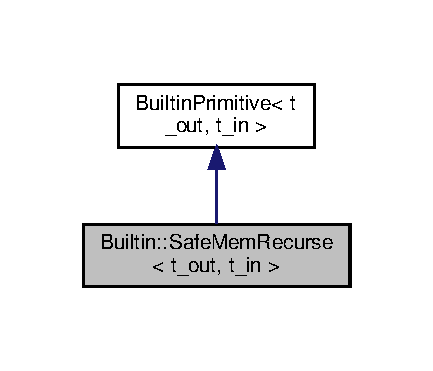
\includegraphics[width=208pt]{struct_builtin_1_1_safe_mem_recurse__inherit__graph}
\end{center}
\end{figure}


Collaboration diagram for Builtin\+:\+:Safe\+Mem\+Recurse$<$ t\+\_\+out, t\+\_\+in $>$\+:\nopagebreak
\begin{figure}[H]
\begin{center}
\leavevmode
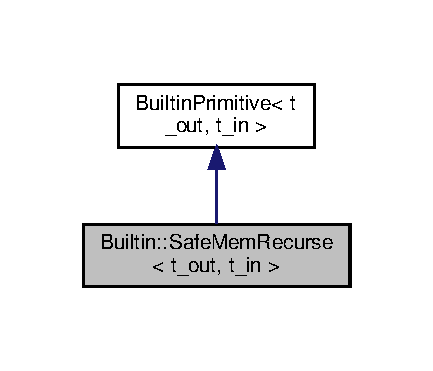
\includegraphics[width=208pt]{struct_builtin_1_1_safe_mem_recurse__coll__graph}
\end{center}
\end{figure}
\subsection*{Public Member Functions}
\begin{DoxyCompactItemize}
\item 
\hyperlink{struct_builtin_1_1_safe_mem_recurse_a1ee433d426eadf08429665c1c6793697}{Safe\+Mem\+Recurse} (std\+::string fmt, double \+\_\+p=1.\+0)
\end{DoxyCompactItemize}
\subsection*{Additional Inherited Members}


\subsection{Constructor \& Destructor Documentation}
\mbox{\Hypertarget{struct_builtin_1_1_safe_mem_recurse_a1ee433d426eadf08429665c1c6793697}\label{struct_builtin_1_1_safe_mem_recurse_a1ee433d426eadf08429665c1c6793697}} 
\index{Builtin\+::\+Safe\+Mem\+Recurse@{Builtin\+::\+Safe\+Mem\+Recurse}!Safe\+Mem\+Recurse@{Safe\+Mem\+Recurse}}
\index{Safe\+Mem\+Recurse@{Safe\+Mem\+Recurse}!Builtin\+::\+Safe\+Mem\+Recurse@{Builtin\+::\+Safe\+Mem\+Recurse}}
\subsubsection{\texorpdfstring{Safe\+Mem\+Recurse()}{SafeMemRecurse()}}
{\footnotesize\ttfamily template$<$typename t\+\_\+out , typename t\+\_\+in $>$ \\
\hyperlink{struct_builtin_1_1_safe_mem_recurse}{Builtin\+::\+Safe\+Mem\+Recurse}$<$ t\+\_\+out, t\+\_\+in $>$\+::\hyperlink{struct_builtin_1_1_safe_mem_recurse}{Safe\+Mem\+Recurse} (\begin{DoxyParamCaption}\item[{std\+::string}]{fmt,  }\item[{double}]{\+\_\+p = {\ttfamily 1.0} }\end{DoxyParamCaption})\hspace{0.3cm}{\ttfamily [inline]}}



The documentation for this struct was generated from the following file\+:\begin{DoxyCompactItemize}
\item 
src/\+Virtual\+Machine/\hyperlink{_builtins_8h}{Builtins.\+h}\end{DoxyCompactItemize}

\hypertarget{struct_builtin_1_1_safe_recurse}{}\section{Builtin\+:\+:Safe\+Recurse$<$ t\+\_\+out, t\+\_\+in $>$ Struct Template Reference}
\label{struct_builtin_1_1_safe_recurse}\index{Builtin\+::\+Safe\+Recurse$<$ t\+\_\+out, t\+\_\+in $>$@{Builtin\+::\+Safe\+Recurse$<$ t\+\_\+out, t\+\_\+in $>$}}


{\ttfamily \#include $<$Builtins.\+h$>$}



Inheritance diagram for Builtin\+:\+:Safe\+Recurse$<$ t\+\_\+out, t\+\_\+in $>$\+:\nopagebreak
\begin{figure}[H]
\begin{center}
\leavevmode
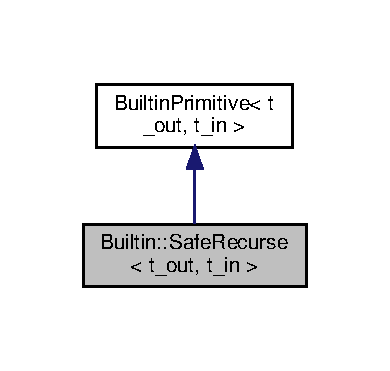
\includegraphics[width=187pt]{struct_builtin_1_1_safe_recurse__inherit__graph}
\end{center}
\end{figure}


Collaboration diagram for Builtin\+:\+:Safe\+Recurse$<$ t\+\_\+out, t\+\_\+in $>$\+:\nopagebreak
\begin{figure}[H]
\begin{center}
\leavevmode
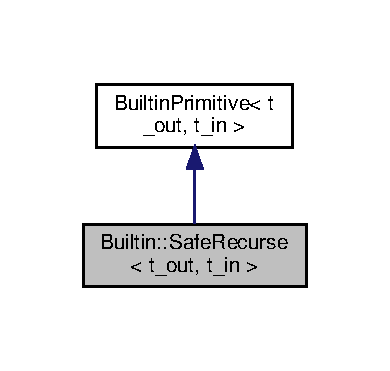
\includegraphics[width=187pt]{struct_builtin_1_1_safe_recurse__coll__graph}
\end{center}
\end{figure}
\subsection*{Public Member Functions}
\begin{DoxyCompactItemize}
\item 
\hyperlink{struct_builtin_1_1_safe_recurse_a08d0badfed57f035599c184302f89304}{Safe\+Recurse} (std\+::string fmt, double \+\_\+p=1.\+0)
\end{DoxyCompactItemize}
\subsection*{Additional Inherited Members}


\subsection{Constructor \& Destructor Documentation}
\mbox{\Hypertarget{struct_builtin_1_1_safe_recurse_a08d0badfed57f035599c184302f89304}\label{struct_builtin_1_1_safe_recurse_a08d0badfed57f035599c184302f89304}} 
\index{Builtin\+::\+Safe\+Recurse@{Builtin\+::\+Safe\+Recurse}!Safe\+Recurse@{Safe\+Recurse}}
\index{Safe\+Recurse@{Safe\+Recurse}!Builtin\+::\+Safe\+Recurse@{Builtin\+::\+Safe\+Recurse}}
\subsubsection{\texorpdfstring{Safe\+Recurse()}{SafeRecurse()}}
{\footnotesize\ttfamily template$<$typename t\+\_\+out , typename t\+\_\+in $>$ \\
\hyperlink{struct_builtin_1_1_safe_recurse}{Builtin\+::\+Safe\+Recurse}$<$ t\+\_\+out, t\+\_\+in $>$\+::\hyperlink{struct_builtin_1_1_safe_recurse}{Safe\+Recurse} (\begin{DoxyParamCaption}\item[{std\+::string}]{fmt,  }\item[{double}]{\+\_\+p = {\ttfamily 1.0} }\end{DoxyParamCaption})\hspace{0.3cm}{\ttfamily [inline]}}



The documentation for this struct was generated from the following file\+:\begin{DoxyCompactItemize}
\item 
src/\+Virtual\+Machine/\hyperlink{_builtins_8h}{Builtins.\+h}\end{DoxyCompactItemize}

\hypertarget{class_searchable}{}\section{Searchable$<$ H\+YP, t\+\_\+input, t\+\_\+output $>$ Class Template Reference}
\label{class_searchable}\index{Searchable$<$ H\+Y\+P, t\+\_\+input, t\+\_\+output $>$@{Searchable$<$ H\+Y\+P, t\+\_\+input, t\+\_\+output $>$}}


{\ttfamily \#include $<$Searchable.\+h$>$}



Inheritance diagram for Searchable$<$ H\+YP, t\+\_\+input, t\+\_\+output $>$\+:\nopagebreak
\begin{figure}[H]
\begin{center}
\leavevmode
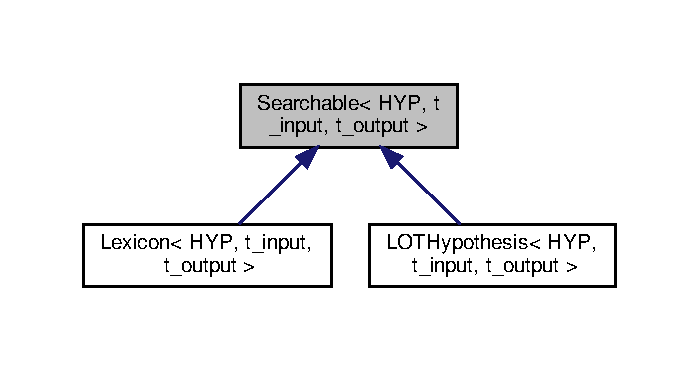
\includegraphics[width=336pt]{class_searchable__inherit__graph}
\end{center}
\end{figure}
\subsection*{Public Member Functions}
\begin{DoxyCompactItemize}
\item 
virtual int \hyperlink{class_searchable_a0450c35a21c5940a63560aa24b4ff0cc}{neighbors} () const =0
\item 
virtual H\+YP \hyperlink{class_searchable_a64bda92cc9314dae7aff31f4444a93e6}{make\+\_\+neighbor} (int k) const =0
\item 
virtual bool \hyperlink{class_searchable_aae16f1cb01f140f4033f6f67dc9753b6}{is\+\_\+evaluable} () const =0
\end{DoxyCompactItemize}


\subsection{Detailed Description}
\subsubsection*{template$<$typename H\+YP, typename t\+\_\+input, typename t\+\_\+output$>$\newline
class Searchable$<$ H\+Y\+P, t\+\_\+input, t\+\_\+output $>$}

\begin{DoxyAuthor}{Author}
steven piantadosi 
\end{DoxyAuthor}
\begin{DoxyDate}{Date}
03/02/20 
\end{DoxyDate}


\subsection{Member Function Documentation}
\mbox{\Hypertarget{class_searchable_aae16f1cb01f140f4033f6f67dc9753b6}\label{class_searchable_aae16f1cb01f140f4033f6f67dc9753b6}} 
\index{Searchable@{Searchable}!is\+\_\+evaluable@{is\+\_\+evaluable}}
\index{is\+\_\+evaluable@{is\+\_\+evaluable}!Searchable@{Searchable}}
\subsubsection{\texorpdfstring{is\+\_\+evaluable()}{is\_evaluable()}}
{\footnotesize\ttfamily template$<$typename H\+YP, typename t\+\_\+input, typename t\+\_\+output$>$ \\
virtual bool \hyperlink{class_searchable}{Searchable}$<$ H\+YP, t\+\_\+input, t\+\_\+output $>$\+::is\+\_\+evaluable (\begin{DoxyParamCaption}{ }\end{DoxyParamCaption}) const\hspace{0.3cm}{\ttfamily [pure virtual]}}



Implemented in \hyperlink{class_lexicon_a4928f2db73eb7d675f347429a4167820}{Lexicon$<$ H\+Y\+P, T, t\+\_\+input, t\+\_\+output, t\+\_\+datum $>$}, \hyperlink{class_lexicon_a4928f2db73eb7d675f347429a4167820}{Lexicon$<$ My\+Hypothesis, Inner\+Hypothesis, S, S $>$}, \hyperlink{class_l_o_t_hypothesis_a68dedaeae92b25b0450f2dc1bd95a35b}{L\+O\+T\+Hypothesis$<$ H\+Y\+P, T, t\+\_\+input, t\+\_\+output, \+\_\+t\+\_\+datum, \+\_\+t\+\_\+data $>$}, \hyperlink{class_l_o_t_hypothesis_a68dedaeae92b25b0450f2dc1bd95a35b}{L\+O\+T\+Hypothesis$<$ Inner\+Hypothesis, Node, S, S $>$}, \hyperlink{class_l_o_t_hypothesis_a68dedaeae92b25b0450f2dc1bd95a35b}{L\+O\+T\+Hypothesis$<$ My\+Hypothesis, Node, Object, bool $>$}, and \hyperlink{class_l_o_t_hypothesis_a68dedaeae92b25b0450f2dc1bd95a35b}{L\+O\+T\+Hypothesis$<$ My\+Hypothesis, Node, float, float, float, std\+::multiset$<$ float $>$ $>$}.

\mbox{\Hypertarget{class_searchable_a64bda92cc9314dae7aff31f4444a93e6}\label{class_searchable_a64bda92cc9314dae7aff31f4444a93e6}} 
\index{Searchable@{Searchable}!make\+\_\+neighbor@{make\+\_\+neighbor}}
\index{make\+\_\+neighbor@{make\+\_\+neighbor}!Searchable@{Searchable}}
\subsubsection{\texorpdfstring{make\+\_\+neighbor()}{make\_neighbor()}}
{\footnotesize\ttfamily template$<$typename H\+YP, typename t\+\_\+input, typename t\+\_\+output$>$ \\
virtual H\+YP \hyperlink{class_searchable}{Searchable}$<$ H\+YP, t\+\_\+input, t\+\_\+output $>$\+::make\+\_\+neighbor (\begin{DoxyParamCaption}\item[{int}]{k }\end{DoxyParamCaption}) const\hspace{0.3cm}{\ttfamily [pure virtual]}}



Implemented in \hyperlink{class_lexicon_a3d4fb7e4545267221eb38acba4d52a6b}{Lexicon$<$ H\+Y\+P, T, t\+\_\+input, t\+\_\+output, t\+\_\+datum $>$}, \hyperlink{class_lexicon_a3d4fb7e4545267221eb38acba4d52a6b}{Lexicon$<$ My\+Hypothesis, Inner\+Hypothesis, S, S $>$}, \hyperlink{class_l_o_t_hypothesis_ae7771176b8b2599f42c75318ee0e9164}{L\+O\+T\+Hypothesis$<$ H\+Y\+P, T, t\+\_\+input, t\+\_\+output, \+\_\+t\+\_\+datum, \+\_\+t\+\_\+data $>$}, \hyperlink{class_l_o_t_hypothesis_ae7771176b8b2599f42c75318ee0e9164}{L\+O\+T\+Hypothesis$<$ Inner\+Hypothesis, Node, S, S $>$}, \hyperlink{class_l_o_t_hypothesis_ae7771176b8b2599f42c75318ee0e9164}{L\+O\+T\+Hypothesis$<$ My\+Hypothesis, Node, Object, bool $>$}, and \hyperlink{class_l_o_t_hypothesis_ae7771176b8b2599f42c75318ee0e9164}{L\+O\+T\+Hypothesis$<$ My\+Hypothesis, Node, float, float, float, std\+::multiset$<$ float $>$ $>$}.

\mbox{\Hypertarget{class_searchable_a0450c35a21c5940a63560aa24b4ff0cc}\label{class_searchable_a0450c35a21c5940a63560aa24b4ff0cc}} 
\index{Searchable@{Searchable}!neighbors@{neighbors}}
\index{neighbors@{neighbors}!Searchable@{Searchable}}
\subsubsection{\texorpdfstring{neighbors()}{neighbors()}}
{\footnotesize\ttfamily template$<$typename H\+YP, typename t\+\_\+input, typename t\+\_\+output$>$ \\
virtual int \hyperlink{class_searchable}{Searchable}$<$ H\+YP, t\+\_\+input, t\+\_\+output $>$\+::neighbors (\begin{DoxyParamCaption}{ }\end{DoxyParamCaption}) const\hspace{0.3cm}{\ttfamily [pure virtual]}}



Implemented in \hyperlink{class_lexicon_abccf49d0f313b9f6e0c3ae286d13ac82}{Lexicon$<$ H\+Y\+P, T, t\+\_\+input, t\+\_\+output, t\+\_\+datum $>$}, \hyperlink{class_lexicon_abccf49d0f313b9f6e0c3ae286d13ac82}{Lexicon$<$ My\+Hypothesis, Inner\+Hypothesis, S, S $>$}, \hyperlink{class_l_o_t_hypothesis_ac74e874f6b677dc1c013602907627be7}{L\+O\+T\+Hypothesis$<$ H\+Y\+P, T, t\+\_\+input, t\+\_\+output, \+\_\+t\+\_\+datum, \+\_\+t\+\_\+data $>$}, \hyperlink{class_l_o_t_hypothesis_ac74e874f6b677dc1c013602907627be7}{L\+O\+T\+Hypothesis$<$ Inner\+Hypothesis, Node, S, S $>$}, \hyperlink{class_l_o_t_hypothesis_ac74e874f6b677dc1c013602907627be7}{L\+O\+T\+Hypothesis$<$ My\+Hypothesis, Node, Object, bool $>$}, and \hyperlink{class_l_o_t_hypothesis_ac74e874f6b677dc1c013602907627be7}{L\+O\+T\+Hypothesis$<$ My\+Hypothesis, Node, float, float, float, std\+::multiset$<$ float $>$ $>$}.



The documentation for this class was generated from the following file\+:\begin{DoxyCompactItemize}
\item 
src/\+Hypotheses/\+Interfaces/\hyperlink{_searchable_8h}{Searchable.\+h}\end{DoxyCompactItemize}

\hypertarget{class_stack}{}\section{Stack$<$ T $>$ Class Template Reference}
\label{class_stack}\index{Stack$<$ T $>$@{Stack$<$ T $>$}}


{\ttfamily \#include $<$Stack.\+h$>$}



Inheritance diagram for Stack$<$ T $>$\+:\nopagebreak
\begin{figure}[H]
\begin{center}
\leavevmode
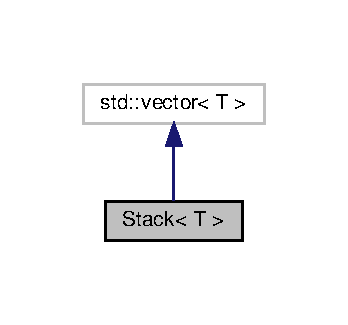
\includegraphics[width=167pt]{class_stack__inherit__graph}
\end{center}
\end{figure}


Collaboration diagram for Stack$<$ T $>$\+:\nopagebreak
\begin{figure}[H]
\begin{center}
\leavevmode
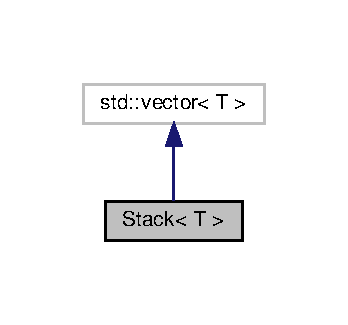
\includegraphics[width=167pt]{class_stack__coll__graph}
\end{center}
\end{figure}
\subsection*{Public Member Functions}
\begin{DoxyCompactItemize}
\item 
\hyperlink{class_stack_aefee698059467258bbd79045aca62a63}{Stack} ()
\item 
void \hyperlink{class_stack_a6e8312460808f468b004d709d3308757}{push} (const T \&val)
\item 
void \hyperlink{class_stack_a2723aec5c7e2611b97fcffeb7709de33}{pop} ()
\item 
T \hyperlink{class_stack_ad461f6de40c8672dbf743068f4515061}{top} ()
\item 
T \& \hyperlink{class_stack_a318da5613921ddf481a21c62ce006c3c}{topref} ()
\end{DoxyCompactItemize}


\subsection{Constructor \& Destructor Documentation}
\mbox{\Hypertarget{class_stack_aefee698059467258bbd79045aca62a63}\label{class_stack_aefee698059467258bbd79045aca62a63}} 
\index{Stack@{Stack}!Stack@{Stack}}
\index{Stack@{Stack}!Stack@{Stack}}
\subsubsection{\texorpdfstring{Stack()}{Stack()}}
{\footnotesize\ttfamily template$<$typename T$>$ \\
\hyperlink{class_stack}{Stack}$<$ T $>$\+::\hyperlink{class_stack}{Stack} (\begin{DoxyParamCaption}{ }\end{DoxyParamCaption})\hspace{0.3cm}{\ttfamily [inline]}}



\subsection{Member Function Documentation}
\mbox{\Hypertarget{class_stack_a2723aec5c7e2611b97fcffeb7709de33}\label{class_stack_a2723aec5c7e2611b97fcffeb7709de33}} 
\index{Stack@{Stack}!pop@{pop}}
\index{pop@{pop}!Stack@{Stack}}
\subsubsection{\texorpdfstring{pop()}{pop()}}
{\footnotesize\ttfamily template$<$typename T$>$ \\
void \hyperlink{class_stack}{Stack}$<$ T $>$\+::pop (\begin{DoxyParamCaption}{ }\end{DoxyParamCaption})\hspace{0.3cm}{\ttfamily [inline]}}

Remove the top element (returning void)\mbox{\Hypertarget{class_stack_a6e8312460808f468b004d709d3308757}\label{class_stack_a6e8312460808f468b004d709d3308757}} 
\index{Stack@{Stack}!push@{push}}
\index{push@{push}!Stack@{Stack}}
\subsubsection{\texorpdfstring{push()}{push()}}
{\footnotesize\ttfamily template$<$typename T$>$ \\
void \hyperlink{class_stack}{Stack}$<$ T $>$\+::push (\begin{DoxyParamCaption}\item[{const T \&}]{val }\end{DoxyParamCaption})\hspace{0.3cm}{\ttfamily [inline]}}

Push val onto the stack 
\begin{DoxyParams}{Parameters}
{\em val} & \\
\hline
\end{DoxyParams}
\mbox{\Hypertarget{class_stack_ad461f6de40c8672dbf743068f4515061}\label{class_stack_ad461f6de40c8672dbf743068f4515061}} 
\index{Stack@{Stack}!top@{top}}
\index{top@{top}!Stack@{Stack}}
\subsubsection{\texorpdfstring{top()}{top()}}
{\footnotesize\ttfamily template$<$typename T$>$ \\
T \hyperlink{class_stack}{Stack}$<$ T $>$\+::top (\begin{DoxyParamCaption}{ }\end{DoxyParamCaption})\hspace{0.3cm}{\ttfamily [inline]}}

Return the top element. \begin{DoxyReturn}{Returns}

\end{DoxyReturn}
\mbox{\Hypertarget{class_stack_a318da5613921ddf481a21c62ce006c3c}\label{class_stack_a318da5613921ddf481a21c62ce006c3c}} 
\index{Stack@{Stack}!topref@{topref}}
\index{topref@{topref}!Stack@{Stack}}
\subsubsection{\texorpdfstring{topref()}{topref()}}
{\footnotesize\ttfamily template$<$typename T$>$ \\
T\& \hyperlink{class_stack}{Stack}$<$ T $>$\+::topref (\begin{DoxyParamCaption}{ }\end{DoxyParamCaption})\hspace{0.3cm}{\ttfamily [inline]}}

Get a reference to the top element (allowing in-\/place modification) \begin{DoxyReturn}{Returns}

\end{DoxyReturn}


The documentation for this class was generated from the following file\+:\begin{DoxyCompactItemize}
\item 
src/\hyperlink{_stack_8h}{Stack.\+h}\end{DoxyCompactItemize}

\hypertarget{class_fleet_1_1_statistics_1_1_streaming_statistics}{}\section{Fleet\+:\+:Statistics\+:\+:Streaming\+Statistics Class Reference}
\label{class_fleet_1_1_statistics_1_1_streaming_statistics}\index{Fleet\+::\+Statistics\+::\+Streaming\+Statistics@{Fleet\+::\+Statistics\+::\+Streaming\+Statistics}}


{\ttfamily \#include $<$Streaming\+Statistics.\+h$>$}



Collaboration diagram for Fleet\+:\+:Statistics\+:\+:Streaming\+Statistics\+:\nopagebreak
\begin{figure}[H]
\begin{center}
\leavevmode
\includegraphics[width=350pt]{class_fleet_1_1_statistics_1_1_streaming_statistics__coll__graph}
\end{center}
\end{figure}
\subsection*{Public Member Functions}
\begin{DoxyCompactItemize}
\item 
\hyperlink{class_fleet_1_1_statistics_1_1_streaming_statistics_a7b22725325625cc7f8c89cce4a19c719}{Streaming\+Statistics} (size\+\_\+t rs=1000)
\item 
void \hyperlink{class_fleet_1_1_statistics_1_1_streaming_statistics_a78daaf22f5e2abd44f82b2e8d2f2cb55}{operator=} (\hyperlink{class_fleet_1_1_statistics_1_1_streaming_statistics}{Streaming\+Statistics} \&\&s)
\item 
void \hyperlink{class_fleet_1_1_statistics_1_1_streaming_statistics_a19575656208452c5ea2bb66257a09c0f}{add} (double x, double lw=0.\+0)
\item 
void \hyperlink{class_fleet_1_1_statistics_1_1_streaming_statistics_af5bcdaff2f20a0048a5b28af8582adf3}{operator$<$$<$} (double x)
\item 
double \hyperlink{class_fleet_1_1_statistics_1_1_streaming_statistics_a65b06c5de083ac12d5b74facd5444973}{sample} () const
\item 
double \hyperlink{class_fleet_1_1_statistics_1_1_streaming_statistics_a70d2554ea987b7e3278b018fdc5ca95a}{median} () const
\item 
void \hyperlink{class_fleet_1_1_statistics_1_1_streaming_statistics_acae72aac2b6ad1ce89e725c001e4e833}{print} () const
\item 
double \hyperlink{class_fleet_1_1_statistics_1_1_streaming_statistics_a0b7d6df2facb2257ec8ef7d4de68fd52}{p\+\_\+exceeds\+\_\+median} (const \hyperlink{class_fleet_1_1_statistics_1_1_streaming_statistics}{Streaming\+Statistics} \&q) const
\end{DoxyCompactItemize}
\subsection*{Public Attributes}
\begin{DoxyCompactItemize}
\item 
double \hyperlink{class_fleet_1_1_statistics_1_1_streaming_statistics_a780941dece7b39cc2feaf7ad95da1ae3}{min}
\item 
double \hyperlink{class_fleet_1_1_statistics_1_1_streaming_statistics_a39d330cb8b112aa23d5460011c161f54}{max}
\item 
double \hyperlink{class_fleet_1_1_statistics_1_1_streaming_statistics_ab635c93398bfd1cc8c0c65b012d87d83}{sum}
\item 
double \hyperlink{class_fleet_1_1_statistics_1_1_streaming_statistics_a4ffa58fb5fd8ce43f06bb8bf56115bd5}{lse}
\item 
double \hyperlink{class_fleet_1_1_statistics_1_1_streaming_statistics_a0ef0c93930850d2f177dca7507fc1831}{N}
\item 
\hyperlink{class_fleet_1_1_statistics_1_1_median_f_a_m_e}{Median\+F\+A\+ME}$<$ double $>$ \hyperlink{class_fleet_1_1_statistics_1_1_streaming_statistics_af01ce0d7840f68c8ea68f858ba6760ce}{streaming\+\_\+median}
\item 
\hyperlink{class_fleet_1_1_statistics_1_1_reservoir_sample}{Reservoir\+Sample}$<$ double $>$ \hyperlink{class_fleet_1_1_statistics_1_1_streaming_statistics_adb520be6722da7da835ac097a5602278}{reservoir\+\_\+sample}
\end{DoxyCompactItemize}
\subsection*{Protected Attributes}
\begin{DoxyCompactItemize}
\item 
std\+::mutex \hyperlink{class_fleet_1_1_statistics_1_1_streaming_statistics_a5651ed8dd36b6586ac64aeb8870d3760}{lock}
\end{DoxyCompactItemize}


\subsection{Detailed Description}
\begin{DoxyAuthor}{Author}
piantado 
\end{DoxyAuthor}
\begin{DoxyDate}{Date}
29/01/20 
\end{DoxyDate}


\subsection{Constructor \& Destructor Documentation}
\mbox{\Hypertarget{class_fleet_1_1_statistics_1_1_streaming_statistics_a7b22725325625cc7f8c89cce4a19c719}\label{class_fleet_1_1_statistics_1_1_streaming_statistics_a7b22725325625cc7f8c89cce4a19c719}} 
\index{Fleet\+::\+Statistics\+::\+Streaming\+Statistics@{Fleet\+::\+Statistics\+::\+Streaming\+Statistics}!Streaming\+Statistics@{Streaming\+Statistics}}
\index{Streaming\+Statistics@{Streaming\+Statistics}!Fleet\+::\+Statistics\+::\+Streaming\+Statistics@{Fleet\+::\+Statistics\+::\+Streaming\+Statistics}}
\subsubsection{\texorpdfstring{Streaming\+Statistics()}{StreamingStatistics()}}
{\footnotesize\ttfamily Fleet\+::\+Statistics\+::\+Streaming\+Statistics\+::\+Streaming\+Statistics (\begin{DoxyParamCaption}\item[{size\+\_\+t}]{rs = {\ttfamily 1000} }\end{DoxyParamCaption})\hspace{0.3cm}{\ttfamily [inline]}}



\subsection{Member Function Documentation}
\mbox{\Hypertarget{class_fleet_1_1_statistics_1_1_streaming_statistics_a19575656208452c5ea2bb66257a09c0f}\label{class_fleet_1_1_statistics_1_1_streaming_statistics_a19575656208452c5ea2bb66257a09c0f}} 
\index{Fleet\+::\+Statistics\+::\+Streaming\+Statistics@{Fleet\+::\+Statistics\+::\+Streaming\+Statistics}!add@{add}}
\index{add@{add}!Fleet\+::\+Statistics\+::\+Streaming\+Statistics@{Fleet\+::\+Statistics\+::\+Streaming\+Statistics}}
\subsubsection{\texorpdfstring{add()}{add()}}
{\footnotesize\ttfamily void Fleet\+::\+Statistics\+::\+Streaming\+Statistics\+::add (\begin{DoxyParamCaption}\item[{double}]{x,  }\item[{double}]{lw = {\ttfamily 0.0} }\end{DoxyParamCaption})\hspace{0.3cm}{\ttfamily [inline]}}

Add sample x (with log weight lw) to these statistics. 
\begin{DoxyParams}{Parameters}
{\em x} & \\
\hline
{\em lw} & \\
\hline
\end{DoxyParams}
\mbox{\Hypertarget{class_fleet_1_1_statistics_1_1_streaming_statistics_a70d2554ea987b7e3278b018fdc5ca95a}\label{class_fleet_1_1_statistics_1_1_streaming_statistics_a70d2554ea987b7e3278b018fdc5ca95a}} 
\index{Fleet\+::\+Statistics\+::\+Streaming\+Statistics@{Fleet\+::\+Statistics\+::\+Streaming\+Statistics}!median@{median}}
\index{median@{median}!Fleet\+::\+Statistics\+::\+Streaming\+Statistics@{Fleet\+::\+Statistics\+::\+Streaming\+Statistics}}
\subsubsection{\texorpdfstring{median()}{median()}}
{\footnotesize\ttfamily double Fleet\+::\+Statistics\+::\+Streaming\+Statistics\+::median (\begin{DoxyParamCaption}{ }\end{DoxyParamCaption}) const\hspace{0.3cm}{\ttfamily [inline]}}

Compute the median according to my reservoir sample. \begin{DoxyReturn}{Returns}

\end{DoxyReturn}
\mbox{\Hypertarget{class_fleet_1_1_statistics_1_1_streaming_statistics_af5bcdaff2f20a0048a5b28af8582adf3}\label{class_fleet_1_1_statistics_1_1_streaming_statistics_af5bcdaff2f20a0048a5b28af8582adf3}} 
\index{Fleet\+::\+Statistics\+::\+Streaming\+Statistics@{Fleet\+::\+Statistics\+::\+Streaming\+Statistics}!operator$<$$<$@{operator$<$$<$}}
\index{operator$<$$<$@{operator$<$$<$}!Fleet\+::\+Statistics\+::\+Streaming\+Statistics@{Fleet\+::\+Statistics\+::\+Streaming\+Statistics}}
\subsubsection{\texorpdfstring{operator$<$$<$()}{operator<<()}}
{\footnotesize\ttfamily void Fleet\+::\+Statistics\+::\+Streaming\+Statistics\+::operator$<$$<$ (\begin{DoxyParamCaption}\item[{double}]{x }\end{DoxyParamCaption})\hspace{0.3cm}{\ttfamily [inline]}}

Add x 
\begin{DoxyParams}{Parameters}
{\em x} & \\
\hline
\end{DoxyParams}
\mbox{\Hypertarget{class_fleet_1_1_statistics_1_1_streaming_statistics_a78daaf22f5e2abd44f82b2e8d2f2cb55}\label{class_fleet_1_1_statistics_1_1_streaming_statistics_a78daaf22f5e2abd44f82b2e8d2f2cb55}} 
\index{Fleet\+::\+Statistics\+::\+Streaming\+Statistics@{Fleet\+::\+Statistics\+::\+Streaming\+Statistics}!operator=@{operator=}}
\index{operator=@{operator=}!Fleet\+::\+Statistics\+::\+Streaming\+Statistics@{Fleet\+::\+Statistics\+::\+Streaming\+Statistics}}
\subsubsection{\texorpdfstring{operator=()}{operator=()}}
{\footnotesize\ttfamily void Fleet\+::\+Statistics\+::\+Streaming\+Statistics\+::operator= (\begin{DoxyParamCaption}\item[{\hyperlink{class_fleet_1_1_statistics_1_1_streaming_statistics}{Streaming\+Statistics} \&\&}]{s }\end{DoxyParamCaption})\hspace{0.3cm}{\ttfamily [inline]}}

\mbox{\Hypertarget{class_fleet_1_1_statistics_1_1_streaming_statistics_a0b7d6df2facb2257ec8ef7d4de68fd52}\label{class_fleet_1_1_statistics_1_1_streaming_statistics_a0b7d6df2facb2257ec8ef7d4de68fd52}} 
\index{Fleet\+::\+Statistics\+::\+Streaming\+Statistics@{Fleet\+::\+Statistics\+::\+Streaming\+Statistics}!p\+\_\+exceeds\+\_\+median@{p\+\_\+exceeds\+\_\+median}}
\index{p\+\_\+exceeds\+\_\+median@{p\+\_\+exceeds\+\_\+median}!Fleet\+::\+Statistics\+::\+Streaming\+Statistics@{Fleet\+::\+Statistics\+::\+Streaming\+Statistics}}
\subsubsection{\texorpdfstring{p\+\_\+exceeds\+\_\+median()}{p\_exceeds\_median()}}
{\footnotesize\ttfamily double Fleet\+::\+Statistics\+::\+Streaming\+Statistics\+::p\+\_\+exceeds\+\_\+median (\begin{DoxyParamCaption}\item[{const \hyperlink{class_fleet_1_1_statistics_1_1_streaming_statistics}{Streaming\+Statistics} \&}]{q }\end{DoxyParamCaption}) const\hspace{0.3cm}{\ttfamily [inline]}}

What proportion of my samples exceed the median of q? 
\begin{DoxyParams}{Parameters}
{\em q} & \\
\hline
\end{DoxyParams}
\begin{DoxyReturn}{Returns}

\end{DoxyReturn}
\mbox{\Hypertarget{class_fleet_1_1_statistics_1_1_streaming_statistics_acae72aac2b6ad1ce89e725c001e4e833}\label{class_fleet_1_1_statistics_1_1_streaming_statistics_acae72aac2b6ad1ce89e725c001e4e833}} 
\index{Fleet\+::\+Statistics\+::\+Streaming\+Statistics@{Fleet\+::\+Statistics\+::\+Streaming\+Statistics}!print@{print}}
\index{print@{print}!Fleet\+::\+Statistics\+::\+Streaming\+Statistics@{Fleet\+::\+Statistics\+::\+Streaming\+Statistics}}
\subsubsection{\texorpdfstring{print()}{print()}}
{\footnotesize\ttfamily void Fleet\+::\+Statistics\+::\+Streaming\+Statistics\+::print (\begin{DoxyParamCaption}{ }\end{DoxyParamCaption}) const\hspace{0.3cm}{\ttfamily [inline]}}

\mbox{\Hypertarget{class_fleet_1_1_statistics_1_1_streaming_statistics_a65b06c5de083ac12d5b74facd5444973}\label{class_fleet_1_1_statistics_1_1_streaming_statistics_a65b06c5de083ac12d5b74facd5444973}} 
\index{Fleet\+::\+Statistics\+::\+Streaming\+Statistics@{Fleet\+::\+Statistics\+::\+Streaming\+Statistics}!sample@{sample}}
\index{sample@{sample}!Fleet\+::\+Statistics\+::\+Streaming\+Statistics@{Fleet\+::\+Statistics\+::\+Streaming\+Statistics}}
\subsubsection{\texorpdfstring{sample()}{sample()}}
{\footnotesize\ttfamily double Fleet\+::\+Statistics\+::\+Streaming\+Statistics\+::sample (\begin{DoxyParamCaption}{ }\end{DoxyParamCaption}) const\hspace{0.3cm}{\ttfamily [inline]}}

Treat as a reservoir sample to sample an element. \begin{DoxyReturn}{Returns}

\end{DoxyReturn}


\subsection{Member Data Documentation}
\mbox{\Hypertarget{class_fleet_1_1_statistics_1_1_streaming_statistics_a5651ed8dd36b6586ac64aeb8870d3760}\label{class_fleet_1_1_statistics_1_1_streaming_statistics_a5651ed8dd36b6586ac64aeb8870d3760}} 
\index{Fleet\+::\+Statistics\+::\+Streaming\+Statistics@{Fleet\+::\+Statistics\+::\+Streaming\+Statistics}!lock@{lock}}
\index{lock@{lock}!Fleet\+::\+Statistics\+::\+Streaming\+Statistics@{Fleet\+::\+Statistics\+::\+Streaming\+Statistics}}
\subsubsection{\texorpdfstring{lock}{lock}}
{\footnotesize\ttfamily std\+::mutex Fleet\+::\+Statistics\+::\+Streaming\+Statistics\+::lock\hspace{0.3cm}{\ttfamily [mutable]}, {\ttfamily [protected]}}

\mbox{\Hypertarget{class_fleet_1_1_statistics_1_1_streaming_statistics_a4ffa58fb5fd8ce43f06bb8bf56115bd5}\label{class_fleet_1_1_statistics_1_1_streaming_statistics_a4ffa58fb5fd8ce43f06bb8bf56115bd5}} 
\index{Fleet\+::\+Statistics\+::\+Streaming\+Statistics@{Fleet\+::\+Statistics\+::\+Streaming\+Statistics}!lse@{lse}}
\index{lse@{lse}!Fleet\+::\+Statistics\+::\+Streaming\+Statistics@{Fleet\+::\+Statistics\+::\+Streaming\+Statistics}}
\subsubsection{\texorpdfstring{lse}{lse}}
{\footnotesize\ttfamily double Fleet\+::\+Statistics\+::\+Streaming\+Statistics\+::lse}

\mbox{\Hypertarget{class_fleet_1_1_statistics_1_1_streaming_statistics_a39d330cb8b112aa23d5460011c161f54}\label{class_fleet_1_1_statistics_1_1_streaming_statistics_a39d330cb8b112aa23d5460011c161f54}} 
\index{Fleet\+::\+Statistics\+::\+Streaming\+Statistics@{Fleet\+::\+Statistics\+::\+Streaming\+Statistics}!max@{max}}
\index{max@{max}!Fleet\+::\+Statistics\+::\+Streaming\+Statistics@{Fleet\+::\+Statistics\+::\+Streaming\+Statistics}}
\subsubsection{\texorpdfstring{max}{max}}
{\footnotesize\ttfamily double Fleet\+::\+Statistics\+::\+Streaming\+Statistics\+::max}

\mbox{\Hypertarget{class_fleet_1_1_statistics_1_1_streaming_statistics_a780941dece7b39cc2feaf7ad95da1ae3}\label{class_fleet_1_1_statistics_1_1_streaming_statistics_a780941dece7b39cc2feaf7ad95da1ae3}} 
\index{Fleet\+::\+Statistics\+::\+Streaming\+Statistics@{Fleet\+::\+Statistics\+::\+Streaming\+Statistics}!min@{min}}
\index{min@{min}!Fleet\+::\+Statistics\+::\+Streaming\+Statistics@{Fleet\+::\+Statistics\+::\+Streaming\+Statistics}}
\subsubsection{\texorpdfstring{min}{min}}
{\footnotesize\ttfamily double Fleet\+::\+Statistics\+::\+Streaming\+Statistics\+::min}

\mbox{\Hypertarget{class_fleet_1_1_statistics_1_1_streaming_statistics_a0ef0c93930850d2f177dca7507fc1831}\label{class_fleet_1_1_statistics_1_1_streaming_statistics_a0ef0c93930850d2f177dca7507fc1831}} 
\index{Fleet\+::\+Statistics\+::\+Streaming\+Statistics@{Fleet\+::\+Statistics\+::\+Streaming\+Statistics}!N@{N}}
\index{N@{N}!Fleet\+::\+Statistics\+::\+Streaming\+Statistics@{Fleet\+::\+Statistics\+::\+Streaming\+Statistics}}
\subsubsection{\texorpdfstring{N}{N}}
{\footnotesize\ttfamily double Fleet\+::\+Statistics\+::\+Streaming\+Statistics\+::N}

\mbox{\Hypertarget{class_fleet_1_1_statistics_1_1_streaming_statistics_adb520be6722da7da835ac097a5602278}\label{class_fleet_1_1_statistics_1_1_streaming_statistics_adb520be6722da7da835ac097a5602278}} 
\index{Fleet\+::\+Statistics\+::\+Streaming\+Statistics@{Fleet\+::\+Statistics\+::\+Streaming\+Statistics}!reservoir\+\_\+sample@{reservoir\+\_\+sample}}
\index{reservoir\+\_\+sample@{reservoir\+\_\+sample}!Fleet\+::\+Statistics\+::\+Streaming\+Statistics@{Fleet\+::\+Statistics\+::\+Streaming\+Statistics}}
\subsubsection{\texorpdfstring{reservoir\+\_\+sample}{reservoir\_sample}}
{\footnotesize\ttfamily \hyperlink{class_fleet_1_1_statistics_1_1_reservoir_sample}{Reservoir\+Sample}$<$double$>$ Fleet\+::\+Statistics\+::\+Streaming\+Statistics\+::reservoir\+\_\+sample}

\mbox{\Hypertarget{class_fleet_1_1_statistics_1_1_streaming_statistics_af01ce0d7840f68c8ea68f858ba6760ce}\label{class_fleet_1_1_statistics_1_1_streaming_statistics_af01ce0d7840f68c8ea68f858ba6760ce}} 
\index{Fleet\+::\+Statistics\+::\+Streaming\+Statistics@{Fleet\+::\+Statistics\+::\+Streaming\+Statistics}!streaming\+\_\+median@{streaming\+\_\+median}}
\index{streaming\+\_\+median@{streaming\+\_\+median}!Fleet\+::\+Statistics\+::\+Streaming\+Statistics@{Fleet\+::\+Statistics\+::\+Streaming\+Statistics}}
\subsubsection{\texorpdfstring{streaming\+\_\+median}{streaming\_median}}
{\footnotesize\ttfamily \hyperlink{class_fleet_1_1_statistics_1_1_median_f_a_m_e}{Median\+F\+A\+ME}$<$double$>$ Fleet\+::\+Statistics\+::\+Streaming\+Statistics\+::streaming\+\_\+median}

\mbox{\Hypertarget{class_fleet_1_1_statistics_1_1_streaming_statistics_ab635c93398bfd1cc8c0c65b012d87d83}\label{class_fleet_1_1_statistics_1_1_streaming_statistics_ab635c93398bfd1cc8c0c65b012d87d83}} 
\index{Fleet\+::\+Statistics\+::\+Streaming\+Statistics@{Fleet\+::\+Statistics\+::\+Streaming\+Statistics}!sum@{sum}}
\index{sum@{sum}!Fleet\+::\+Statistics\+::\+Streaming\+Statistics@{Fleet\+::\+Statistics\+::\+Streaming\+Statistics}}
\subsubsection{\texorpdfstring{sum}{sum}}
{\footnotesize\ttfamily double Fleet\+::\+Statistics\+::\+Streaming\+Statistics\+::sum}



The documentation for this class was generated from the following file\+:\begin{DoxyCompactItemize}
\item 
src/\+Statistics/\hyperlink{_streaming_statistics_8h}{Streaming\+Statistics.\+h}\end{DoxyCompactItemize}

\hypertarget{structt__null}{}\section{t\+\_\+null Struct Reference}
\label{structt__null}\index{t\+\_\+null@{t\+\_\+null}}


{\ttfamily \#include $<$Miscellaneous.\+h$>$}



The documentation for this struct was generated from the following file\+:\begin{DoxyCompactItemize}
\item 
src/\hyperlink{_miscellaneous_8h}{Miscellaneous.\+h}\end{DoxyCompactItemize}

\hypertarget{struct_virtual_machine_state_1_1t__stack}{}\section{Virtual\+Machine\+State$<$ t\+\_\+x, t\+\_\+return $>$\+:\+:t\+\_\+stack$<$ args $>$ Struct Template Reference}
\label{struct_virtual_machine_state_1_1t__stack}\index{Virtual\+Machine\+State$<$ t\+\_\+x, t\+\_\+return $>$\+::t\+\_\+stack$<$ args $>$@{Virtual\+Machine\+State$<$ t\+\_\+x, t\+\_\+return $>$\+::t\+\_\+stack$<$ args $>$}}


{\ttfamily \#include $<$Virtual\+Machine\+State.\+h$>$}

\subsection*{Public Attributes}
\begin{DoxyCompactItemize}
\item 
std\+::tuple$<$ \hyperlink{class_stack}{Stack}$<$ args $>$... $>$ \hyperlink{struct_virtual_machine_state_1_1t__stack_a455e35013f15a7e7b328da628d711e49}{value}
\end{DoxyCompactItemize}


\subsection{Member Data Documentation}
\mbox{\Hypertarget{struct_virtual_machine_state_1_1t__stack_a455e35013f15a7e7b328da628d711e49}\label{struct_virtual_machine_state_1_1t__stack_a455e35013f15a7e7b328da628d711e49}} 
\index{Virtual\+Machine\+State\+::t\+\_\+stack@{Virtual\+Machine\+State\+::t\+\_\+stack}!value@{value}}
\index{value@{value}!Virtual\+Machine\+State\+::t\+\_\+stack@{Virtual\+Machine\+State\+::t\+\_\+stack}}
\subsubsection{\texorpdfstring{value}{value}}
{\footnotesize\ttfamily template$<$typename t\+\_\+x, typename t\+\_\+return$>$ \\
template$<$typename... args$>$ \\
std\+::tuple$<$\hyperlink{class_stack}{Stack}$<$args$>$...$>$ \hyperlink{class_virtual_machine_state}{Virtual\+Machine\+State}$<$ t\+\_\+x, t\+\_\+return $>$\+::\hyperlink{struct_virtual_machine_state_1_1t__stack}{t\+\_\+stack}$<$ args $>$\+::value}



The documentation for this struct was generated from the following file\+:\begin{DoxyCompactItemize}
\item 
src/\+Virtual\+Machine/\hyperlink{_virtual_machine_state_8h}{Virtual\+Machine\+State.\+h}\end{DoxyCompactItemize}

\hypertarget{class_fleet_1_1_statistics_1_1_top_n}{}\section{Fleet\+:\+:Statistics\+:\+:TopN$<$ T $>$ Class Template Reference}
\label{class_fleet_1_1_statistics_1_1_top_n}\index{Fleet\+::\+Statistics\+::\+Top\+N$<$ T $>$@{Fleet\+::\+Statistics\+::\+Top\+N$<$ T $>$}}


{\ttfamily \#include $<$Top.\+h$>$}

\subsection*{Public Member Functions}
\begin{DoxyCompactItemize}
\item 
\hyperlink{class_fleet_1_1_statistics_1_1_top_n_afd0ca4daca84e66e91a4101cb009af44}{TopN} (size\+\_\+t n=std\+::numeric\+\_\+limits$<$ size\+\_\+t $>$\+::max())
\item 
\hyperlink{class_fleet_1_1_statistics_1_1_top_n_a3c7b5c9c3fd6e171a0b2d6b1f48cddf3}{TopN} (const \hyperlink{class_fleet_1_1_statistics_1_1_top_n}{TopN}$<$ T $>$ \&x)
\item 
\hyperlink{class_fleet_1_1_statistics_1_1_top_n_af1a27643fa0841afaa7e8ca0e87d9a49}{TopN} (\hyperlink{class_fleet_1_1_statistics_1_1_top_n}{TopN}$<$ T $>$ \&\&x)
\item 
void \hyperlink{class_fleet_1_1_statistics_1_1_top_n_a38d3aba302a215992c603ff2ab13e8fc}{operator=} (const \hyperlink{class_fleet_1_1_statistics_1_1_top_n}{TopN}$<$ T $>$ \&x)
\item 
void \hyperlink{class_fleet_1_1_statistics_1_1_top_n_a6653acde6effd65aa0226cbefc2c8f4f}{operator=} (\hyperlink{class_fleet_1_1_statistics_1_1_top_n}{TopN}$<$ T $>$ \&\&x)
\item 
void \hyperlink{class_fleet_1_1_statistics_1_1_top_n_a3151da8c2aaab75195d6f702fbfba436}{set\+\_\+size} (size\+\_\+t n)
\item 
void \hyperlink{class_fleet_1_1_statistics_1_1_top_n_a762c937fe5dcab09d87d2414201b6b1e}{set\+\_\+print\+\_\+best} (bool b)
\item 
size\+\_\+t \hyperlink{class_fleet_1_1_statistics_1_1_top_n_a0ce96f95fbac59ba2a858b66b5a6690a}{size} () const
\item 
bool \hyperlink{class_fleet_1_1_statistics_1_1_top_n_ac2b70eef6c75a0459acc88b2539dbc0b}{empty} () const
\item 
const std\+::multiset$<$ T $>$ \& \hyperlink{class_fleet_1_1_statistics_1_1_top_n_ab7ab88abe1dd8afe6ffecf9206cbceb7}{values} () const
\item 
void \hyperlink{class_fleet_1_1_statistics_1_1_top_n_a71f34724832a34c029bfeeb6e1dea24f}{add} (const T \&x, size\+\_\+t \hyperlink{class_fleet_1_1_statistics_1_1_top_n_a341df027d3283fe3a9bf3766521e126d}{count}=1)
\item 
void \hyperlink{class_fleet_1_1_statistics_1_1_top_n_af54651d8e83bdcc6b3ffbcef3aa3fd6e}{operator$<$$<$} (const T \&x)
\item 
void \hyperlink{class_fleet_1_1_statistics_1_1_top_n_ac1a720c5f52f0486377274bd1e6a052a}{add} (const \hyperlink{class_fleet_1_1_statistics_1_1_top_n}{TopN}$<$ T $>$ \&x)
\item 
void \hyperlink{class_fleet_1_1_statistics_1_1_top_n_a73cb4911b6dc2bdc56f466ca4b93ef9d}{operator$<$$<$} (const \hyperlink{class_fleet_1_1_statistics_1_1_top_n}{TopN}$<$ T $>$ \&x)
\item 
void \hyperlink{class_fleet_1_1_statistics_1_1_top_n_a3300639fe8eef303fb66e1630dc0790c}{operator()} (T \&x)
\item 
size\+\_\+t \hyperlink{class_fleet_1_1_statistics_1_1_top_n_acb11e623b45dbec10f2c1ac9a48b0eef}{operator\mbox{[}$\,$\mbox{]}} (const T \&x)
\item 
const T \& \hyperlink{class_fleet_1_1_statistics_1_1_top_n_a61aa70a203ecf97f79d26cb4bcfe2071}{best} ()
\item 
const T \& \hyperlink{class_fleet_1_1_statistics_1_1_top_n_a7be596fb7defba492b503371c58b30ce}{worst} ()
\item 
double \hyperlink{class_fleet_1_1_statistics_1_1_top_n_aa94e0f1e4df0ba70b35abcc540b7cb03}{Z} ()
\item 
void \hyperlink{class_fleet_1_1_statistics_1_1_top_n_ae37eb4f39eb12d32a1f04aa30276da86}{print} (std\+::string prefix=\char`\"{}\char`\"{})
\item 
void \hyperlink{class_fleet_1_1_statistics_1_1_top_n_ab57188b1858802dcf1f26dbcf702c6ae}{clear} ()
\item 
unsigned long \hyperlink{class_fleet_1_1_statistics_1_1_top_n_a341df027d3283fe3a9bf3766521e126d}{count} (const T x)
\item 
{\footnotesize template$<$typename t\+\_\+data $>$ }\\\hyperlink{class_fleet_1_1_statistics_1_1_top_n}{TopN} \hyperlink{class_fleet_1_1_statistics_1_1_top_n_ac6ab403d6833e58352e24110ee379fbf}{compute\+\_\+posterior} (t\+\_\+data \&data)
\end{DoxyCompactItemize}
\subsection*{Public Attributes}
\begin{DoxyCompactItemize}
\item 
std\+::map$<$ T, unsigned long $>$ \hyperlink{class_fleet_1_1_statistics_1_1_top_n_a0f5ecded3f85aeeb85da2f2b3056b466}{cnt}
\item 
std\+::multiset$<$ T $>$ \hyperlink{class_fleet_1_1_statistics_1_1_top_n_aa17d03f1154073197161f59657d4c80b}{s}
\item 
bool \hyperlink{class_fleet_1_1_statistics_1_1_top_n_a1ee284a643f14a5c4670b4c5f61f5262}{print\+\_\+best}
\item 
std\+::atomic$<$ size\+\_\+t $>$ \hyperlink{class_fleet_1_1_statistics_1_1_top_n_a7a9612e75b42451eef7db77498050e7a}{N}
\end{DoxyCompactItemize}


\subsection{Detailed Description}
\subsubsection*{template$<$class T$>$\newline
class Fleet\+::\+Statistics\+::\+Top\+N$<$ T $>$}

\begin{DoxyAuthor}{Author}
steven piantadosi 
\end{DoxyAuthor}
\begin{DoxyDate}{Date}
03/02/20 
\end{DoxyDate}


\subsection{Constructor \& Destructor Documentation}
\mbox{\Hypertarget{class_fleet_1_1_statistics_1_1_top_n_afd0ca4daca84e66e91a4101cb009af44}\label{class_fleet_1_1_statistics_1_1_top_n_afd0ca4daca84e66e91a4101cb009af44}} 
\index{Fleet\+::\+Statistics\+::\+TopN@{Fleet\+::\+Statistics\+::\+TopN}!TopN@{TopN}}
\index{TopN@{TopN}!Fleet\+::\+Statistics\+::\+TopN@{Fleet\+::\+Statistics\+::\+TopN}}
\subsubsection{\texorpdfstring{Top\+N()}{TopN()}\hspace{0.1cm}{\footnotesize\ttfamily [1/3]}}
{\footnotesize\ttfamily template$<$class T$>$ \\
\hyperlink{class_fleet_1_1_statistics_1_1_top_n}{Fleet\+::\+Statistics\+::\+TopN}$<$ T $>$\+::\hyperlink{class_fleet_1_1_statistics_1_1_top_n}{TopN} (\begin{DoxyParamCaption}\item[{size\+\_\+t}]{n = {\ttfamily std\+:\+:numeric\+\_\+limits$<$size\+\_\+t$>$\+:\+:max()} }\end{DoxyParamCaption})\hspace{0.3cm}{\ttfamily [inline]}}

\mbox{\Hypertarget{class_fleet_1_1_statistics_1_1_top_n_a3c7b5c9c3fd6e171a0b2d6b1f48cddf3}\label{class_fleet_1_1_statistics_1_1_top_n_a3c7b5c9c3fd6e171a0b2d6b1f48cddf3}} 
\index{Fleet\+::\+Statistics\+::\+TopN@{Fleet\+::\+Statistics\+::\+TopN}!TopN@{TopN}}
\index{TopN@{TopN}!Fleet\+::\+Statistics\+::\+TopN@{Fleet\+::\+Statistics\+::\+TopN}}
\subsubsection{\texorpdfstring{Top\+N()}{TopN()}\hspace{0.1cm}{\footnotesize\ttfamily [2/3]}}
{\footnotesize\ttfamily template$<$class T$>$ \\
\hyperlink{class_fleet_1_1_statistics_1_1_top_n}{Fleet\+::\+Statistics\+::\+TopN}$<$ T $>$\+::\hyperlink{class_fleet_1_1_statistics_1_1_top_n}{TopN} (\begin{DoxyParamCaption}\item[{const \hyperlink{class_fleet_1_1_statistics_1_1_top_n}{TopN}$<$ T $>$ \&}]{x }\end{DoxyParamCaption})\hspace{0.3cm}{\ttfamily [inline]}}

\mbox{\Hypertarget{class_fleet_1_1_statistics_1_1_top_n_af1a27643fa0841afaa7e8ca0e87d9a49}\label{class_fleet_1_1_statistics_1_1_top_n_af1a27643fa0841afaa7e8ca0e87d9a49}} 
\index{Fleet\+::\+Statistics\+::\+TopN@{Fleet\+::\+Statistics\+::\+TopN}!TopN@{TopN}}
\index{TopN@{TopN}!Fleet\+::\+Statistics\+::\+TopN@{Fleet\+::\+Statistics\+::\+TopN}}
\subsubsection{\texorpdfstring{Top\+N()}{TopN()}\hspace{0.1cm}{\footnotesize\ttfamily [3/3]}}
{\footnotesize\ttfamily template$<$class T$>$ \\
\hyperlink{class_fleet_1_1_statistics_1_1_top_n}{Fleet\+::\+Statistics\+::\+TopN}$<$ T $>$\+::\hyperlink{class_fleet_1_1_statistics_1_1_top_n}{TopN} (\begin{DoxyParamCaption}\item[{\hyperlink{class_fleet_1_1_statistics_1_1_top_n}{TopN}$<$ T $>$ \&\&}]{x }\end{DoxyParamCaption})\hspace{0.3cm}{\ttfamily [inline]}}



\subsection{Member Function Documentation}
\mbox{\Hypertarget{class_fleet_1_1_statistics_1_1_top_n_a71f34724832a34c029bfeeb6e1dea24f}\label{class_fleet_1_1_statistics_1_1_top_n_a71f34724832a34c029bfeeb6e1dea24f}} 
\index{Fleet\+::\+Statistics\+::\+TopN@{Fleet\+::\+Statistics\+::\+TopN}!add@{add}}
\index{add@{add}!Fleet\+::\+Statistics\+::\+TopN@{Fleet\+::\+Statistics\+::\+TopN}}
\subsubsection{\texorpdfstring{add()}{add()}\hspace{0.1cm}{\footnotesize\ttfamily [1/2]}}
{\footnotesize\ttfamily template$<$class T$>$ \\
void \hyperlink{class_fleet_1_1_statistics_1_1_top_n}{Fleet\+::\+Statistics\+::\+TopN}$<$ T $>$\+::add (\begin{DoxyParamCaption}\item[{const T \&}]{x,  }\item[{size\+\_\+t}]{count = {\ttfamily 1} }\end{DoxyParamCaption})\hspace{0.3cm}{\ttfamily [inline]}}

Add x. If count is set, that will add that many counts. N\+O\+TE that we do not add objects x such that x.\+posterior == -\/infinity or NaN 
\begin{DoxyParams}{Parameters}
{\em x} & \\
\hline
{\em count} & \\
\hline
\end{DoxyParams}
\mbox{\Hypertarget{class_fleet_1_1_statistics_1_1_top_n_ac1a720c5f52f0486377274bd1e6a052a}\label{class_fleet_1_1_statistics_1_1_top_n_ac1a720c5f52f0486377274bd1e6a052a}} 
\index{Fleet\+::\+Statistics\+::\+TopN@{Fleet\+::\+Statistics\+::\+TopN}!add@{add}}
\index{add@{add}!Fleet\+::\+Statistics\+::\+TopN@{Fleet\+::\+Statistics\+::\+TopN}}
\subsubsection{\texorpdfstring{add()}{add()}\hspace{0.1cm}{\footnotesize\ttfamily [2/2]}}
{\footnotesize\ttfamily template$<$class T$>$ \\
void \hyperlink{class_fleet_1_1_statistics_1_1_top_n}{Fleet\+::\+Statistics\+::\+TopN}$<$ T $>$\+::add (\begin{DoxyParamCaption}\item[{const \hyperlink{class_fleet_1_1_statistics_1_1_top_n}{TopN}$<$ T $>$ \&}]{x }\end{DoxyParamCaption})\hspace{0.3cm}{\ttfamily [inline]}}

Add everything in x to this one. 
\begin{DoxyParams}{Parameters}
{\em x} & \\
\hline
\end{DoxyParams}
\mbox{\Hypertarget{class_fleet_1_1_statistics_1_1_top_n_a61aa70a203ecf97f79d26cb4bcfe2071}\label{class_fleet_1_1_statistics_1_1_top_n_a61aa70a203ecf97f79d26cb4bcfe2071}} 
\index{Fleet\+::\+Statistics\+::\+TopN@{Fleet\+::\+Statistics\+::\+TopN}!best@{best}}
\index{best@{best}!Fleet\+::\+Statistics\+::\+TopN@{Fleet\+::\+Statistics\+::\+TopN}}
\subsubsection{\texorpdfstring{best()}{best()}}
{\footnotesize\ttfamily template$<$class T$>$ \\
const T\& \hyperlink{class_fleet_1_1_statistics_1_1_top_n}{Fleet\+::\+Statistics\+::\+TopN}$<$ T $>$\+::best (\begin{DoxyParamCaption}{ }\end{DoxyParamCaption})\hspace{0.3cm}{\ttfamily [inline]}}

Returns a reference to the best element currently stored \begin{DoxyReturn}{Returns}

\end{DoxyReturn}
\mbox{\Hypertarget{class_fleet_1_1_statistics_1_1_top_n_ab57188b1858802dcf1f26dbcf702c6ae}\label{class_fleet_1_1_statistics_1_1_top_n_ab57188b1858802dcf1f26dbcf702c6ae}} 
\index{Fleet\+::\+Statistics\+::\+TopN@{Fleet\+::\+Statistics\+::\+TopN}!clear@{clear}}
\index{clear@{clear}!Fleet\+::\+Statistics\+::\+TopN@{Fleet\+::\+Statistics\+::\+TopN}}
\subsubsection{\texorpdfstring{clear()}{clear()}}
{\footnotesize\ttfamily template$<$class T$>$ \\
void \hyperlink{class_fleet_1_1_statistics_1_1_top_n}{Fleet\+::\+Statistics\+::\+TopN}$<$ T $>$\+::clear (\begin{DoxyParamCaption}{ }\end{DoxyParamCaption})\hspace{0.3cm}{\ttfamily [inline]}}

Remove everything\mbox{\Hypertarget{class_fleet_1_1_statistics_1_1_top_n_ac6ab403d6833e58352e24110ee379fbf}\label{class_fleet_1_1_statistics_1_1_top_n_ac6ab403d6833e58352e24110ee379fbf}} 
\index{Fleet\+::\+Statistics\+::\+TopN@{Fleet\+::\+Statistics\+::\+TopN}!compute\+\_\+posterior@{compute\+\_\+posterior}}
\index{compute\+\_\+posterior@{compute\+\_\+posterior}!Fleet\+::\+Statistics\+::\+TopN@{Fleet\+::\+Statistics\+::\+TopN}}
\subsubsection{\texorpdfstring{compute\+\_\+posterior()}{compute\_posterior()}}
{\footnotesize\ttfamily template$<$class T$>$ \\
template$<$typename t\+\_\+data $>$ \\
\hyperlink{class_fleet_1_1_statistics_1_1_top_n}{TopN} \hyperlink{class_fleet_1_1_statistics_1_1_top_n}{Fleet\+::\+Statistics\+::\+TopN}$<$ T $>$\+::compute\+\_\+posterior (\begin{DoxyParamCaption}\item[{t\+\_\+data \&}]{data }\end{DoxyParamCaption})\hspace{0.3cm}{\ttfamily [inline]}}

Returns a N\+EW \hyperlink{class_fleet_1_1_statistics_1_1_top_n}{TopN} where each current hypothesis is evaluated on the data. N\+O\+TE\+: If a hypothesis has a new posterior of -\/inf or NaN, it won\textquotesingle{}t be added. 
\begin{DoxyParams}{Parameters}
{\em data} & \\
\hline
\end{DoxyParams}
\begin{DoxyReturn}{Returns}

\end{DoxyReturn}
\mbox{\Hypertarget{class_fleet_1_1_statistics_1_1_top_n_a341df027d3283fe3a9bf3766521e126d}\label{class_fleet_1_1_statistics_1_1_top_n_a341df027d3283fe3a9bf3766521e126d}} 
\index{Fleet\+::\+Statistics\+::\+TopN@{Fleet\+::\+Statistics\+::\+TopN}!count@{count}}
\index{count@{count}!Fleet\+::\+Statistics\+::\+TopN@{Fleet\+::\+Statistics\+::\+TopN}}
\subsubsection{\texorpdfstring{count()}{count()}}
{\footnotesize\ttfamily template$<$class T$>$ \\
unsigned long \hyperlink{class_fleet_1_1_statistics_1_1_top_n}{Fleet\+::\+Statistics\+::\+TopN}$<$ T $>$\+::count (\begin{DoxyParamCaption}\item[{const T}]{x }\end{DoxyParamCaption})\hspace{0.3cm}{\ttfamily [inline]}}

How many times have we seen x? 
\begin{DoxyParams}{Parameters}
{\em x} & \\
\hline
\end{DoxyParams}
\begin{DoxyReturn}{Returns}

\end{DoxyReturn}
\mbox{\Hypertarget{class_fleet_1_1_statistics_1_1_top_n_ac2b70eef6c75a0459acc88b2539dbc0b}\label{class_fleet_1_1_statistics_1_1_top_n_ac2b70eef6c75a0459acc88b2539dbc0b}} 
\index{Fleet\+::\+Statistics\+::\+TopN@{Fleet\+::\+Statistics\+::\+TopN}!empty@{empty}}
\index{empty@{empty}!Fleet\+::\+Statistics\+::\+TopN@{Fleet\+::\+Statistics\+::\+TopN}}
\subsubsection{\texorpdfstring{empty()}{empty()}}
{\footnotesize\ttfamily template$<$class T$>$ \\
bool \hyperlink{class_fleet_1_1_statistics_1_1_top_n}{Fleet\+::\+Statistics\+::\+TopN}$<$ T $>$\+::empty (\begin{DoxyParamCaption}{ }\end{DoxyParamCaption}) const\hspace{0.3cm}{\ttfamily [inline]}}

Is it empty? \begin{DoxyReturn}{Returns}

\end{DoxyReturn}
\mbox{\Hypertarget{class_fleet_1_1_statistics_1_1_top_n_a3300639fe8eef303fb66e1630dc0790c}\label{class_fleet_1_1_statistics_1_1_top_n_a3300639fe8eef303fb66e1630dc0790c}} 
\index{Fleet\+::\+Statistics\+::\+TopN@{Fleet\+::\+Statistics\+::\+TopN}!operator()@{operator()}}
\index{operator()@{operator()}!Fleet\+::\+Statistics\+::\+TopN@{Fleet\+::\+Statistics\+::\+TopN}}
\subsubsection{\texorpdfstring{operator()()}{operator()()}}
{\footnotesize\ttfamily template$<$class T$>$ \\
void \hyperlink{class_fleet_1_1_statistics_1_1_top_n}{Fleet\+::\+Statistics\+::\+TopN}$<$ T $>$\+::operator() (\begin{DoxyParamCaption}\item[{T \&}]{x }\end{DoxyParamCaption})\hspace{0.3cm}{\ttfamily [inline]}}

\mbox{\Hypertarget{class_fleet_1_1_statistics_1_1_top_n_af54651d8e83bdcc6b3ffbcef3aa3fd6e}\label{class_fleet_1_1_statistics_1_1_top_n_af54651d8e83bdcc6b3ffbcef3aa3fd6e}} 
\index{Fleet\+::\+Statistics\+::\+TopN@{Fleet\+::\+Statistics\+::\+TopN}!operator$<$$<$@{operator$<$$<$}}
\index{operator$<$$<$@{operator$<$$<$}!Fleet\+::\+Statistics\+::\+TopN@{Fleet\+::\+Statistics\+::\+TopN}}
\subsubsection{\texorpdfstring{operator$<$$<$()}{operator<<()}\hspace{0.1cm}{\footnotesize\ttfamily [1/2]}}
{\footnotesize\ttfamily template$<$class T$>$ \\
void \hyperlink{class_fleet_1_1_statistics_1_1_top_n}{Fleet\+::\+Statistics\+::\+TopN}$<$ T $>$\+::operator$<$$<$ (\begin{DoxyParamCaption}\item[{const T \&}]{x }\end{DoxyParamCaption})\hspace{0.3cm}{\ttfamily [inline]}}

Friendlier syntax for adding. 
\begin{DoxyParams}{Parameters}
{\em x} & \\
\hline
\end{DoxyParams}
\mbox{\Hypertarget{class_fleet_1_1_statistics_1_1_top_n_a73cb4911b6dc2bdc56f466ca4b93ef9d}\label{class_fleet_1_1_statistics_1_1_top_n_a73cb4911b6dc2bdc56f466ca4b93ef9d}} 
\index{Fleet\+::\+Statistics\+::\+TopN@{Fleet\+::\+Statistics\+::\+TopN}!operator$<$$<$@{operator$<$$<$}}
\index{operator$<$$<$@{operator$<$$<$}!Fleet\+::\+Statistics\+::\+TopN@{Fleet\+::\+Statistics\+::\+TopN}}
\subsubsection{\texorpdfstring{operator$<$$<$()}{operator<<()}\hspace{0.1cm}{\footnotesize\ttfamily [2/2]}}
{\footnotesize\ttfamily template$<$class T$>$ \\
void \hyperlink{class_fleet_1_1_statistics_1_1_top_n}{Fleet\+::\+Statistics\+::\+TopN}$<$ T $>$\+::operator$<$$<$ (\begin{DoxyParamCaption}\item[{const \hyperlink{class_fleet_1_1_statistics_1_1_top_n}{TopN}$<$ T $>$ \&}]{x }\end{DoxyParamCaption})\hspace{0.3cm}{\ttfamily [inline]}}

\mbox{\Hypertarget{class_fleet_1_1_statistics_1_1_top_n_a38d3aba302a215992c603ff2ab13e8fc}\label{class_fleet_1_1_statistics_1_1_top_n_a38d3aba302a215992c603ff2ab13e8fc}} 
\index{Fleet\+::\+Statistics\+::\+TopN@{Fleet\+::\+Statistics\+::\+TopN}!operator=@{operator=}}
\index{operator=@{operator=}!Fleet\+::\+Statistics\+::\+TopN@{Fleet\+::\+Statistics\+::\+TopN}}
\subsubsection{\texorpdfstring{operator=()}{operator=()}\hspace{0.1cm}{\footnotesize\ttfamily [1/2]}}
{\footnotesize\ttfamily template$<$class T$>$ \\
void \hyperlink{class_fleet_1_1_statistics_1_1_top_n}{Fleet\+::\+Statistics\+::\+TopN}$<$ T $>$\+::operator= (\begin{DoxyParamCaption}\item[{const \hyperlink{class_fleet_1_1_statistics_1_1_top_n}{TopN}$<$ T $>$ \&}]{x }\end{DoxyParamCaption})\hspace{0.3cm}{\ttfamily [inline]}}

\mbox{\Hypertarget{class_fleet_1_1_statistics_1_1_top_n_a6653acde6effd65aa0226cbefc2c8f4f}\label{class_fleet_1_1_statistics_1_1_top_n_a6653acde6effd65aa0226cbefc2c8f4f}} 
\index{Fleet\+::\+Statistics\+::\+TopN@{Fleet\+::\+Statistics\+::\+TopN}!operator=@{operator=}}
\index{operator=@{operator=}!Fleet\+::\+Statistics\+::\+TopN@{Fleet\+::\+Statistics\+::\+TopN}}
\subsubsection{\texorpdfstring{operator=()}{operator=()}\hspace{0.1cm}{\footnotesize\ttfamily [2/2]}}
{\footnotesize\ttfamily template$<$class T$>$ \\
void \hyperlink{class_fleet_1_1_statistics_1_1_top_n}{Fleet\+::\+Statistics\+::\+TopN}$<$ T $>$\+::operator= (\begin{DoxyParamCaption}\item[{\hyperlink{class_fleet_1_1_statistics_1_1_top_n}{TopN}$<$ T $>$ \&\&}]{x }\end{DoxyParamCaption})\hspace{0.3cm}{\ttfamily [inline]}}

\mbox{\Hypertarget{class_fleet_1_1_statistics_1_1_top_n_acb11e623b45dbec10f2c1ac9a48b0eef}\label{class_fleet_1_1_statistics_1_1_top_n_acb11e623b45dbec10f2c1ac9a48b0eef}} 
\index{Fleet\+::\+Statistics\+::\+TopN@{Fleet\+::\+Statistics\+::\+TopN}!operator\mbox{[}\mbox{]}@{operator[]}}
\index{operator\mbox{[}\mbox{]}@{operator[]}!Fleet\+::\+Statistics\+::\+TopN@{Fleet\+::\+Statistics\+::\+TopN}}
\subsubsection{\texorpdfstring{operator[]()}{operator[]()}}
{\footnotesize\ttfamily template$<$class T$>$ \\
size\+\_\+t \hyperlink{class_fleet_1_1_statistics_1_1_top_n}{Fleet\+::\+Statistics\+::\+TopN}$<$ T $>$\+::operator\mbox{[}$\,$\mbox{]} (\begin{DoxyParamCaption}\item[{const T \&}]{x }\end{DoxyParamCaption})\hspace{0.3cm}{\ttfamily [inline]}}

Access the counts for a given element x 
\begin{DoxyParams}{Parameters}
{\em x} & \\
\hline
\end{DoxyParams}
\begin{DoxyReturn}{Returns}

\end{DoxyReturn}
\mbox{\Hypertarget{class_fleet_1_1_statistics_1_1_top_n_ae37eb4f39eb12d32a1f04aa30276da86}\label{class_fleet_1_1_statistics_1_1_top_n_ae37eb4f39eb12d32a1f04aa30276da86}} 
\index{Fleet\+::\+Statistics\+::\+TopN@{Fleet\+::\+Statistics\+::\+TopN}!print@{print}}
\index{print@{print}!Fleet\+::\+Statistics\+::\+TopN@{Fleet\+::\+Statistics\+::\+TopN}}
\subsubsection{\texorpdfstring{print()}{print()}}
{\footnotesize\ttfamily template$<$class T$>$ \\
void \hyperlink{class_fleet_1_1_statistics_1_1_top_n}{Fleet\+::\+Statistics\+::\+TopN}$<$ T $>$\+::print (\begin{DoxyParamCaption}\item[{std\+::string}]{prefix = {\ttfamily \char`\"{}\char`\"{}} }\end{DoxyParamCaption})\hspace{0.3cm}{\ttfamily [inline]}}

Sort and print from worst to best 
\begin{DoxyParams}{Parameters}
{\em prefix} & -\/ an optional prefix to print before each line\\
\hline
\end{DoxyParams}
\mbox{\Hypertarget{class_fleet_1_1_statistics_1_1_top_n_a762c937fe5dcab09d87d2414201b6b1e}\label{class_fleet_1_1_statistics_1_1_top_n_a762c937fe5dcab09d87d2414201b6b1e}} 
\index{Fleet\+::\+Statistics\+::\+TopN@{Fleet\+::\+Statistics\+::\+TopN}!set\+\_\+print\+\_\+best@{set\+\_\+print\+\_\+best}}
\index{set\+\_\+print\+\_\+best@{set\+\_\+print\+\_\+best}!Fleet\+::\+Statistics\+::\+TopN@{Fleet\+::\+Statistics\+::\+TopN}}
\subsubsection{\texorpdfstring{set\+\_\+print\+\_\+best()}{set\_print\_best()}}
{\footnotesize\ttfamily template$<$class T$>$ \\
void \hyperlink{class_fleet_1_1_statistics_1_1_top_n}{Fleet\+::\+Statistics\+::\+TopN}$<$ T $>$\+::set\+\_\+print\+\_\+best (\begin{DoxyParamCaption}\item[{bool}]{b }\end{DoxyParamCaption})\hspace{0.3cm}{\ttfamily [inline]}}

As I add things, should I print the best I\textquotesingle{}ve seen so far? 
\begin{DoxyParams}{Parameters}
{\em b} & \\
\hline
\end{DoxyParams}
\mbox{\Hypertarget{class_fleet_1_1_statistics_1_1_top_n_a3151da8c2aaab75195d6f702fbfba436}\label{class_fleet_1_1_statistics_1_1_top_n_a3151da8c2aaab75195d6f702fbfba436}} 
\index{Fleet\+::\+Statistics\+::\+TopN@{Fleet\+::\+Statistics\+::\+TopN}!set\+\_\+size@{set\+\_\+size}}
\index{set\+\_\+size@{set\+\_\+size}!Fleet\+::\+Statistics\+::\+TopN@{Fleet\+::\+Statistics\+::\+TopN}}
\subsubsection{\texorpdfstring{set\+\_\+size()}{set\_size()}}
{\footnotesize\ttfamily template$<$class T$>$ \\
void \hyperlink{class_fleet_1_1_statistics_1_1_top_n}{Fleet\+::\+Statistics\+::\+TopN}$<$ T $>$\+::set\+\_\+size (\begin{DoxyParamCaption}\item[{size\+\_\+t}]{n }\end{DoxyParamCaption})\hspace{0.3cm}{\ttfamily [inline]}}

Set the size of n that I cna have. N\+O\+TE\+: this does not resize the existing data. 
\begin{DoxyParams}{Parameters}
{\em n} & \\
\hline
\end{DoxyParams}
\mbox{\Hypertarget{class_fleet_1_1_statistics_1_1_top_n_a0ce96f95fbac59ba2a858b66b5a6690a}\label{class_fleet_1_1_statistics_1_1_top_n_a0ce96f95fbac59ba2a858b66b5a6690a}} 
\index{Fleet\+::\+Statistics\+::\+TopN@{Fleet\+::\+Statistics\+::\+TopN}!size@{size}}
\index{size@{size}!Fleet\+::\+Statistics\+::\+TopN@{Fleet\+::\+Statistics\+::\+TopN}}
\subsubsection{\texorpdfstring{size()}{size()}}
{\footnotesize\ttfamily template$<$class T$>$ \\
size\+\_\+t \hyperlink{class_fleet_1_1_statistics_1_1_top_n}{Fleet\+::\+Statistics\+::\+TopN}$<$ T $>$\+::size (\begin{DoxyParamCaption}{ }\end{DoxyParamCaption}) const\hspace{0.3cm}{\ttfamily [inline]}}

How many are currently in the set? (N\+OT the total number allowed) \begin{DoxyReturn}{Returns}

\end{DoxyReturn}
\mbox{\Hypertarget{class_fleet_1_1_statistics_1_1_top_n_ab7ab88abe1dd8afe6ffecf9206cbceb7}\label{class_fleet_1_1_statistics_1_1_top_n_ab7ab88abe1dd8afe6ffecf9206cbceb7}} 
\index{Fleet\+::\+Statistics\+::\+TopN@{Fleet\+::\+Statistics\+::\+TopN}!values@{values}}
\index{values@{values}!Fleet\+::\+Statistics\+::\+TopN@{Fleet\+::\+Statistics\+::\+TopN}}
\subsubsection{\texorpdfstring{values()}{values()}}
{\footnotesize\ttfamily template$<$class T$>$ \\
const std\+::multiset$<$T$>$\& \hyperlink{class_fleet_1_1_statistics_1_1_top_n}{Fleet\+::\+Statistics\+::\+TopN}$<$ T $>$\+::values (\begin{DoxyParamCaption}{ }\end{DoxyParamCaption}) const\hspace{0.3cm}{\ttfamily [inline]}}

Return a multiset of all the values in \hyperlink{class_fleet_1_1_statistics_1_1_top_n}{TopN} \begin{DoxyReturn}{Returns}

\end{DoxyReturn}
\mbox{\Hypertarget{class_fleet_1_1_statistics_1_1_top_n_a7be596fb7defba492b503371c58b30ce}\label{class_fleet_1_1_statistics_1_1_top_n_a7be596fb7defba492b503371c58b30ce}} 
\index{Fleet\+::\+Statistics\+::\+TopN@{Fleet\+::\+Statistics\+::\+TopN}!worst@{worst}}
\index{worst@{worst}!Fleet\+::\+Statistics\+::\+TopN@{Fleet\+::\+Statistics\+::\+TopN}}
\subsubsection{\texorpdfstring{worst()}{worst()}}
{\footnotesize\ttfamily template$<$class T$>$ \\
const T\& \hyperlink{class_fleet_1_1_statistics_1_1_top_n}{Fleet\+::\+Statistics\+::\+TopN}$<$ T $>$\+::worst (\begin{DoxyParamCaption}{ }\end{DoxyParamCaption})\hspace{0.3cm}{\ttfamily [inline]}}

Returns a reference to the worst element currently stored \begin{DoxyReturn}{Returns}

\end{DoxyReturn}
\mbox{\Hypertarget{class_fleet_1_1_statistics_1_1_top_n_aa94e0f1e4df0ba70b35abcc540b7cb03}\label{class_fleet_1_1_statistics_1_1_top_n_aa94e0f1e4df0ba70b35abcc540b7cb03}} 
\index{Fleet\+::\+Statistics\+::\+TopN@{Fleet\+::\+Statistics\+::\+TopN}!Z@{Z}}
\index{Z@{Z}!Fleet\+::\+Statistics\+::\+TopN@{Fleet\+::\+Statistics\+::\+TopN}}
\subsubsection{\texorpdfstring{Z()}{Z()}}
{\footnotesize\ttfamily template$<$class T$>$ \\
double \hyperlink{class_fleet_1_1_statistics_1_1_top_n}{Fleet\+::\+Statistics\+::\+TopN}$<$ T $>$\+::Z (\begin{DoxyParamCaption}{ }\end{DoxyParamCaption})\hspace{0.3cm}{\ttfamily [inline]}}

Compute the logsumexp of all of the elements stored. \begin{DoxyReturn}{Returns}

\end{DoxyReturn}


\subsection{Member Data Documentation}
\mbox{\Hypertarget{class_fleet_1_1_statistics_1_1_top_n_a0f5ecded3f85aeeb85da2f2b3056b466}\label{class_fleet_1_1_statistics_1_1_top_n_a0f5ecded3f85aeeb85da2f2b3056b466}} 
\index{Fleet\+::\+Statistics\+::\+TopN@{Fleet\+::\+Statistics\+::\+TopN}!cnt@{cnt}}
\index{cnt@{cnt}!Fleet\+::\+Statistics\+::\+TopN@{Fleet\+::\+Statistics\+::\+TopN}}
\subsubsection{\texorpdfstring{cnt}{cnt}}
{\footnotesize\ttfamily template$<$class T$>$ \\
std\+::map$<$T,unsigned long$>$ \hyperlink{class_fleet_1_1_statistics_1_1_top_n}{Fleet\+::\+Statistics\+::\+TopN}$<$ T $>$\+::cnt}

\mbox{\Hypertarget{class_fleet_1_1_statistics_1_1_top_n_a7a9612e75b42451eef7db77498050e7a}\label{class_fleet_1_1_statistics_1_1_top_n_a7a9612e75b42451eef7db77498050e7a}} 
\index{Fleet\+::\+Statistics\+::\+TopN@{Fleet\+::\+Statistics\+::\+TopN}!N@{N}}
\index{N@{N}!Fleet\+::\+Statistics\+::\+TopN@{Fleet\+::\+Statistics\+::\+TopN}}
\subsubsection{\texorpdfstring{N}{N}}
{\footnotesize\ttfamily template$<$class T$>$ \\
std\+::atomic$<$size\+\_\+t$>$ \hyperlink{class_fleet_1_1_statistics_1_1_top_n}{Fleet\+::\+Statistics\+::\+TopN}$<$ T $>$\+::N}

\mbox{\Hypertarget{class_fleet_1_1_statistics_1_1_top_n_a1ee284a643f14a5c4670b4c5f61f5262}\label{class_fleet_1_1_statistics_1_1_top_n_a1ee284a643f14a5c4670b4c5f61f5262}} 
\index{Fleet\+::\+Statistics\+::\+TopN@{Fleet\+::\+Statistics\+::\+TopN}!print\+\_\+best@{print\+\_\+best}}
\index{print\+\_\+best@{print\+\_\+best}!Fleet\+::\+Statistics\+::\+TopN@{Fleet\+::\+Statistics\+::\+TopN}}
\subsubsection{\texorpdfstring{print\+\_\+best}{print\_best}}
{\footnotesize\ttfamily template$<$class T$>$ \\
bool \hyperlink{class_fleet_1_1_statistics_1_1_top_n}{Fleet\+::\+Statistics\+::\+TopN}$<$ T $>$\+::print\+\_\+best}

\mbox{\Hypertarget{class_fleet_1_1_statistics_1_1_top_n_aa17d03f1154073197161f59657d4c80b}\label{class_fleet_1_1_statistics_1_1_top_n_aa17d03f1154073197161f59657d4c80b}} 
\index{Fleet\+::\+Statistics\+::\+TopN@{Fleet\+::\+Statistics\+::\+TopN}!s@{s}}
\index{s@{s}!Fleet\+::\+Statistics\+::\+TopN@{Fleet\+::\+Statistics\+::\+TopN}}
\subsubsection{\texorpdfstring{s}{s}}
{\footnotesize\ttfamily template$<$class T$>$ \\
std\+::multiset$<$T$>$ \hyperlink{class_fleet_1_1_statistics_1_1_top_n}{Fleet\+::\+Statistics\+::\+TopN}$<$ T $>$\+::s}



The documentation for this class was generated from the following file\+:\begin{DoxyCompactItemize}
\item 
src/\+Statistics/\hyperlink{_top_8h}{Top.\+h}\end{DoxyCompactItemize}

\input{struct_type_index}
\input{struct_type_index_3_01_t_00_01std_1_1tuple_3_01_t_00_01_types_8_8_8_01_4_01_4}
\input{struct_type_index_3_01_t_00_01std_1_1tuple_3_01_u_00_01_types_8_8_8_01_4_01_4}
\hypertarget{class_virtual_machine_pool}{}\section{Virtual\+Machine\+Pool$<$ t\+\_\+x, t\+\_\+return $>$ Class Template Reference}
\label{class_virtual_machine_pool}\index{Virtual\+Machine\+Pool$<$ t\+\_\+x, t\+\_\+return $>$@{Virtual\+Machine\+Pool$<$ t\+\_\+x, t\+\_\+return $>$}}


{\ttfamily \#include $<$Dispatchable.\+h$>$}

\subsection*{Public Member Functions}
\begin{DoxyCompactItemize}
\item 
\hyperlink{class_virtual_machine_pool_abe43be5b1c5e9c1305b237a4a2bd209b}{Virtual\+Machine\+Pool} (unsigned long ms=2048, unsigned long mo=256, double mlp=-\/20)
\item 
virtual \hyperlink{class_virtual_machine_pool_a8fd087ac2d947b46b4be4d5e1baf1682}{$\sim$\+Virtual\+Machine\+Pool} ()
\item 
bool \hyperlink{class_virtual_machine_pool_a4313a26d5523b4ad07927c9de2344c2e}{would\+Iadd} (double lp)
\item 
void \hyperlink{class_virtual_machine_pool_a6f49ab47e6d472b5a9f429e96364b4c6}{push} (\hyperlink{class_virtual_machine_state}{V\+M\+State} $\ast$o)
\item 
{\footnotesize template$<$typename T $>$ }\\bool \hyperlink{class_virtual_machine_pool_a022aad4a11f24264fd7d11060d041852}{copy\+\_\+increment\+\_\+push} (const \hyperlink{class_virtual_machine_state}{V\+M\+State} $\ast$x, T v, double lpinc)
\item 
{\footnotesize template$<$typename T $>$ }\\bool \hyperlink{class_virtual_machine_pool_a3997e8c0a6581b5f68f6ff568dbb53e4}{increment\+\_\+push} (\hyperlink{class_virtual_machine_state}{V\+M\+State} $\ast$s, T v, double lpinc)
\item 
\hyperlink{class_discrete_distribution}{Discrete\+Distribution}$<$ t\+\_\+return $>$ \hyperlink{class_virtual_machine_pool_afee0d242681df11e7ecded1c31f37669}{run} (\hyperlink{class_dispatchable}{Dispatchable}$<$ t\+\_\+x, t\+\_\+return $>$ $\ast$dispatcher, \hyperlink{class_dispatchable}{Dispatchable}$<$ t\+\_\+x, t\+\_\+return $>$ $\ast$loader)
\end{DoxyCompactItemize}
\subsection*{Public Attributes}
\begin{DoxyCompactItemize}
\item 
const unsigned long \hyperlink{class_virtual_machine_pool_ae87303ebbcbff239ff4f3217087420a9}{max\+\_\+steps}
\item 
const unsigned long \hyperlink{class_virtual_machine_pool_ad32df5f3c78137c35a4fcc22916c8598}{max\+\_\+outputs}
\item 
unsigned long \hyperlink{class_virtual_machine_pool_a31cd55d7c9c7daf930bcc7f57b67d930}{current\+\_\+steps}
\item 
double \hyperlink{class_virtual_machine_pool_a3705ed3241bdd47aa2e585cfd67509d6}{min\+\_\+lp}
\item 
double \hyperlink{class_virtual_machine_pool_a9d5d6a1e078b9790f4193af8845d060f}{worst\+\_\+lp} = \hyperlink{_numerics_8h_a1bb1e42ae1b40cad6e99da0aab8a5576}{infinity}
\item 
std\+::priority\+\_\+queue$<$ \hyperlink{class_virtual_machine_state}{V\+M\+State} $\ast$, std\+::vector$<$ \hyperlink{class_virtual_machine_state}{V\+M\+State} $\ast$ $>$, Virtual\+Machine\+Pool\+::compare\+\_\+\+V\+M\+State\+\_\+prt $>$ \hyperlink{class_virtual_machine_pool_aab39827c242ded3fcc4675d2c24687a7}{Q}
\end{DoxyCompactItemize}


\subsection{Detailed Description}
\subsubsection*{template$<$typename t\+\_\+x, typename t\+\_\+return$>$\newline
class Virtual\+Machine\+Pool$<$ t\+\_\+x, t\+\_\+return $>$}

\begin{DoxyAuthor}{Author}
piantado 
\end{DoxyAuthor}
\begin{DoxyDate}{Date}
02/02/20 
\end{DoxyDate}


\subsection{Constructor \& Destructor Documentation}
\mbox{\Hypertarget{class_virtual_machine_pool_abe43be5b1c5e9c1305b237a4a2bd209b}\label{class_virtual_machine_pool_abe43be5b1c5e9c1305b237a4a2bd209b}} 
\index{Virtual\+Machine\+Pool@{Virtual\+Machine\+Pool}!Virtual\+Machine\+Pool@{Virtual\+Machine\+Pool}}
\index{Virtual\+Machine\+Pool@{Virtual\+Machine\+Pool}!Virtual\+Machine\+Pool@{Virtual\+Machine\+Pool}}
\subsubsection{\texorpdfstring{Virtual\+Machine\+Pool()}{VirtualMachinePool()}}
{\footnotesize\ttfamily template$<$typename t\+\_\+x, typename t\+\_\+return$>$ \\
\hyperlink{class_virtual_machine_pool}{Virtual\+Machine\+Pool}$<$ t\+\_\+x, t\+\_\+return $>$\+::\hyperlink{class_virtual_machine_pool}{Virtual\+Machine\+Pool} (\begin{DoxyParamCaption}\item[{unsigned long}]{ms = {\ttfamily 2048},  }\item[{unsigned long}]{mo = {\ttfamily 256},  }\item[{double}]{mlp = {\ttfamily -\/20} }\end{DoxyParamCaption})\hspace{0.3cm}{\ttfamily [inline]}}

\mbox{\Hypertarget{class_virtual_machine_pool_a8fd087ac2d947b46b4be4d5e1baf1682}\label{class_virtual_machine_pool_a8fd087ac2d947b46b4be4d5e1baf1682}} 
\index{Virtual\+Machine\+Pool@{Virtual\+Machine\+Pool}!````~Virtual\+Machine\+Pool@{$\sim$\+Virtual\+Machine\+Pool}}
\index{````~Virtual\+Machine\+Pool@{$\sim$\+Virtual\+Machine\+Pool}!Virtual\+Machine\+Pool@{Virtual\+Machine\+Pool}}
\subsubsection{\texorpdfstring{$\sim$\+Virtual\+Machine\+Pool()}{~VirtualMachinePool()}}
{\footnotesize\ttfamily template$<$typename t\+\_\+x, typename t\+\_\+return$>$ \\
virtual \hyperlink{class_virtual_machine_pool}{Virtual\+Machine\+Pool}$<$ t\+\_\+x, t\+\_\+return $>$\+::$\sim$\hyperlink{class_virtual_machine_pool}{Virtual\+Machine\+Pool} (\begin{DoxyParamCaption}{ }\end{DoxyParamCaption})\hspace{0.3cm}{\ttfamily [inline]}, {\ttfamily [virtual]}}



\subsection{Member Function Documentation}
\mbox{\Hypertarget{class_virtual_machine_pool_a022aad4a11f24264fd7d11060d041852}\label{class_virtual_machine_pool_a022aad4a11f24264fd7d11060d041852}} 
\index{Virtual\+Machine\+Pool@{Virtual\+Machine\+Pool}!copy\+\_\+increment\+\_\+push@{copy\+\_\+increment\+\_\+push}}
\index{copy\+\_\+increment\+\_\+push@{copy\+\_\+increment\+\_\+push}!Virtual\+Machine\+Pool@{Virtual\+Machine\+Pool}}
\subsubsection{\texorpdfstring{copy\+\_\+increment\+\_\+push()}{copy\_increment\_push()}}
{\footnotesize\ttfamily template$<$typename t\+\_\+x, typename t\+\_\+return$>$ \\
template$<$typename T $>$ \\
bool \hyperlink{class_virtual_machine_pool}{Virtual\+Machine\+Pool}$<$ t\+\_\+x, t\+\_\+return $>$\+::copy\+\_\+increment\+\_\+push (\begin{DoxyParamCaption}\item[{const \hyperlink{class_virtual_machine_state}{V\+M\+State} $\ast$}]{x,  }\item[{T}]{v,  }\item[{double}]{lpinc }\end{DoxyParamCaption})\hspace{0.3cm}{\ttfamily [inline]}}

This is an important opimization where we will make a copy of x, push v into it\textquotesingle{}s stack, and increment its lp by lpinc only if it will be added to the queue, which we check in the pool here. This saves us from having to use the \hyperlink{class_virtual_machine_state}{Virtual\+Machine\+State} constructor (e.\+g. making a copy, which is expensive if we are copying all the stacks) if the copy won\textquotesingle{}t actually be added to the queue. 
\begin{DoxyParams}{Parameters}
{\em x} & \\
\hline
{\em v} & \\
\hline
{\em lpinc} & \\
\hline
\end{DoxyParams}
\begin{DoxyReturn}{Returns}

\end{DoxyReturn}
\mbox{\Hypertarget{class_virtual_machine_pool_a3997e8c0a6581b5f68f6ff568dbb53e4}\label{class_virtual_machine_pool_a3997e8c0a6581b5f68f6ff568dbb53e4}} 
\index{Virtual\+Machine\+Pool@{Virtual\+Machine\+Pool}!increment\+\_\+push@{increment\+\_\+push}}
\index{increment\+\_\+push@{increment\+\_\+push}!Virtual\+Machine\+Pool@{Virtual\+Machine\+Pool}}
\subsubsection{\texorpdfstring{increment\+\_\+push()}{increment\_push()}}
{\footnotesize\ttfamily template$<$typename t\+\_\+x, typename t\+\_\+return$>$ \\
template$<$typename T $>$ \\
bool \hyperlink{class_virtual_machine_pool}{Virtual\+Machine\+Pool}$<$ t\+\_\+x, t\+\_\+return $>$\+::increment\+\_\+push (\begin{DoxyParamCaption}\item[{\hyperlink{class_virtual_machine_state}{V\+M\+State} $\ast$}]{s,  }\item[{T}]{v,  }\item[{double}]{lpinc }\end{DoxyParamCaption})\hspace{0.3cm}{\ttfamily [inline]}}

Same as copy\+\_\+increment\+\_\+push, but does not make a copy -- just add 
\begin{DoxyParams}{Parameters}
{\em s} & \\
\hline
{\em v} & \\
\hline
{\em lpinc} & \\
\hline
\end{DoxyParams}
\begin{DoxyReturn}{Returns}

\end{DoxyReturn}
\mbox{\Hypertarget{class_virtual_machine_pool_a6f49ab47e6d472b5a9f429e96364b4c6}\label{class_virtual_machine_pool_a6f49ab47e6d472b5a9f429e96364b4c6}} 
\index{Virtual\+Machine\+Pool@{Virtual\+Machine\+Pool}!push@{push}}
\index{push@{push}!Virtual\+Machine\+Pool@{Virtual\+Machine\+Pool}}
\subsubsection{\texorpdfstring{push()}{push()}}
{\footnotesize\ttfamily template$<$typename t\+\_\+x, typename t\+\_\+return$>$ \\
void \hyperlink{class_virtual_machine_pool}{Virtual\+Machine\+Pool}$<$ t\+\_\+x, t\+\_\+return $>$\+::push (\begin{DoxyParamCaption}\item[{\hyperlink{class_virtual_machine_state}{V\+M\+State} $\ast$}]{o }\end{DoxyParamCaption})\hspace{0.3cm}{\ttfamily [inline]}}

Add the V\+M\+State o to this pool (but again checking if I\textquotesingle{}d add) 
\begin{DoxyParams}{Parameters}
{\em o} & \\
\hline
\end{DoxyParams}
\mbox{\Hypertarget{class_virtual_machine_pool_afee0d242681df11e7ecded1c31f37669}\label{class_virtual_machine_pool_afee0d242681df11e7ecded1c31f37669}} 
\index{Virtual\+Machine\+Pool@{Virtual\+Machine\+Pool}!run@{run}}
\index{run@{run}!Virtual\+Machine\+Pool@{Virtual\+Machine\+Pool}}
\subsubsection{\texorpdfstring{run()}{run()}}
{\footnotesize\ttfamily template$<$typename t\+\_\+x, typename t\+\_\+return$>$ \\
\hyperlink{class_discrete_distribution}{Discrete\+Distribution}$<$t\+\_\+return$>$ \hyperlink{class_virtual_machine_pool}{Virtual\+Machine\+Pool}$<$ t\+\_\+x, t\+\_\+return $>$\+::run (\begin{DoxyParamCaption}\item[{\hyperlink{class_dispatchable}{Dispatchable}$<$ t\+\_\+x, t\+\_\+return $>$ $\ast$}]{dispatcher,  }\item[{\hyperlink{class_dispatchable}{Dispatchable}$<$ t\+\_\+x, t\+\_\+return $>$ $\ast$}]{loader }\end{DoxyParamCaption})\hspace{0.3cm}{\ttfamily [inline]}}

This runs and adds up the probability mass for everything, returning a dictionary outcomes-\/$>$log\+\_\+probabilities. This is the main running loop, which pops frmo the top of our queue, runs, and continues until we\textquotesingle{}ve done enough or all. Note that objects lower than min\+\_\+lp are not ever pushed onto the queue. 
\begin{DoxyParams}{Parameters}
{\em dispatcher} & \\
\hline
{\em loader} & \\
\hline
\end{DoxyParams}
\begin{DoxyReturn}{Returns}

\end{DoxyReturn}
\mbox{\Hypertarget{class_virtual_machine_pool_a4313a26d5523b4ad07927c9de2344c2e}\label{class_virtual_machine_pool_a4313a26d5523b4ad07927c9de2344c2e}} 
\index{Virtual\+Machine\+Pool@{Virtual\+Machine\+Pool}!would\+Iadd@{would\+Iadd}}
\index{would\+Iadd@{would\+Iadd}!Virtual\+Machine\+Pool@{Virtual\+Machine\+Pool}}
\subsubsection{\texorpdfstring{would\+Iadd()}{wouldIadd()}}
{\footnotesize\ttfamily template$<$typename t\+\_\+x, typename t\+\_\+return$>$ \\
bool \hyperlink{class_virtual_machine_pool}{Virtual\+Machine\+Pool}$<$ t\+\_\+x, t\+\_\+return $>$\+::would\+Iadd (\begin{DoxyParamCaption}\item[{double}]{lp }\end{DoxyParamCaption})\hspace{0.3cm}{\ttfamily [inline]}}

Returns true if I would add something with this lp, given my max\+\_\+steps and the stack. This lets us speed up by checking if we would add before copying/constructing a V\+MS 
\begin{DoxyParams}{Parameters}
{\em lp} & \\
\hline
\end{DoxyParams}
\begin{DoxyReturn}{Returns}

\end{DoxyReturn}


\subsection{Member Data Documentation}
\mbox{\Hypertarget{class_virtual_machine_pool_a31cd55d7c9c7daf930bcc7f57b67d930}\label{class_virtual_machine_pool_a31cd55d7c9c7daf930bcc7f57b67d930}} 
\index{Virtual\+Machine\+Pool@{Virtual\+Machine\+Pool}!current\+\_\+steps@{current\+\_\+steps}}
\index{current\+\_\+steps@{current\+\_\+steps}!Virtual\+Machine\+Pool@{Virtual\+Machine\+Pool}}
\subsubsection{\texorpdfstring{current\+\_\+steps}{current\_steps}}
{\footnotesize\ttfamily template$<$typename t\+\_\+x, typename t\+\_\+return$>$ \\
unsigned long \hyperlink{class_virtual_machine_pool}{Virtual\+Machine\+Pool}$<$ t\+\_\+x, t\+\_\+return $>$\+::current\+\_\+steps}

\mbox{\Hypertarget{class_virtual_machine_pool_ad32df5f3c78137c35a4fcc22916c8598}\label{class_virtual_machine_pool_ad32df5f3c78137c35a4fcc22916c8598}} 
\index{Virtual\+Machine\+Pool@{Virtual\+Machine\+Pool}!max\+\_\+outputs@{max\+\_\+outputs}}
\index{max\+\_\+outputs@{max\+\_\+outputs}!Virtual\+Machine\+Pool@{Virtual\+Machine\+Pool}}
\subsubsection{\texorpdfstring{max\+\_\+outputs}{max\_outputs}}
{\footnotesize\ttfamily template$<$typename t\+\_\+x, typename t\+\_\+return$>$ \\
const unsigned long \hyperlink{class_virtual_machine_pool}{Virtual\+Machine\+Pool}$<$ t\+\_\+x, t\+\_\+return $>$\+::max\+\_\+outputs}

\mbox{\Hypertarget{class_virtual_machine_pool_ae87303ebbcbff239ff4f3217087420a9}\label{class_virtual_machine_pool_ae87303ebbcbff239ff4f3217087420a9}} 
\index{Virtual\+Machine\+Pool@{Virtual\+Machine\+Pool}!max\+\_\+steps@{max\+\_\+steps}}
\index{max\+\_\+steps@{max\+\_\+steps}!Virtual\+Machine\+Pool@{Virtual\+Machine\+Pool}}
\subsubsection{\texorpdfstring{max\+\_\+steps}{max\_steps}}
{\footnotesize\ttfamily template$<$typename t\+\_\+x, typename t\+\_\+return$>$ \\
const unsigned long \hyperlink{class_virtual_machine_pool}{Virtual\+Machine\+Pool}$<$ t\+\_\+x, t\+\_\+return $>$\+::max\+\_\+steps}

\mbox{\Hypertarget{class_virtual_machine_pool_a3705ed3241bdd47aa2e585cfd67509d6}\label{class_virtual_machine_pool_a3705ed3241bdd47aa2e585cfd67509d6}} 
\index{Virtual\+Machine\+Pool@{Virtual\+Machine\+Pool}!min\+\_\+lp@{min\+\_\+lp}}
\index{min\+\_\+lp@{min\+\_\+lp}!Virtual\+Machine\+Pool@{Virtual\+Machine\+Pool}}
\subsubsection{\texorpdfstring{min\+\_\+lp}{min\_lp}}
{\footnotesize\ttfamily template$<$typename t\+\_\+x, typename t\+\_\+return$>$ \\
double \hyperlink{class_virtual_machine_pool}{Virtual\+Machine\+Pool}$<$ t\+\_\+x, t\+\_\+return $>$\+::min\+\_\+lp}

\mbox{\Hypertarget{class_virtual_machine_pool_aab39827c242ded3fcc4675d2c24687a7}\label{class_virtual_machine_pool_aab39827c242ded3fcc4675d2c24687a7}} 
\index{Virtual\+Machine\+Pool@{Virtual\+Machine\+Pool}!Q@{Q}}
\index{Q@{Q}!Virtual\+Machine\+Pool@{Virtual\+Machine\+Pool}}
\subsubsection{\texorpdfstring{Q}{Q}}
{\footnotesize\ttfamily template$<$typename t\+\_\+x, typename t\+\_\+return$>$ \\
std\+::priority\+\_\+queue$<$\hyperlink{class_virtual_machine_state}{V\+M\+State}$\ast$, std\+::vector$<$\hyperlink{class_virtual_machine_state}{V\+M\+State}$\ast$$>$, Virtual\+Machine\+Pool\+::compare\+\_\+\+V\+M\+State\+\_\+prt$>$ \hyperlink{class_virtual_machine_pool}{Virtual\+Machine\+Pool}$<$ t\+\_\+x, t\+\_\+return $>$\+::Q}

\mbox{\Hypertarget{class_virtual_machine_pool_a9d5d6a1e078b9790f4193af8845d060f}\label{class_virtual_machine_pool_a9d5d6a1e078b9790f4193af8845d060f}} 
\index{Virtual\+Machine\+Pool@{Virtual\+Machine\+Pool}!worst\+\_\+lp@{worst\+\_\+lp}}
\index{worst\+\_\+lp@{worst\+\_\+lp}!Virtual\+Machine\+Pool@{Virtual\+Machine\+Pool}}
\subsubsection{\texorpdfstring{worst\+\_\+lp}{worst\_lp}}
{\footnotesize\ttfamily template$<$typename t\+\_\+x, typename t\+\_\+return$>$ \\
double \hyperlink{class_virtual_machine_pool}{Virtual\+Machine\+Pool}$<$ t\+\_\+x, t\+\_\+return $>$\+::worst\+\_\+lp = \hyperlink{_numerics_8h_a1bb1e42ae1b40cad6e99da0aab8a5576}{infinity}}



The documentation for this class was generated from the following files\+:\begin{DoxyCompactItemize}
\item 
src/\+Hypotheses/\+Interfaces/\hyperlink{_dispatchable_8h}{Dispatchable.\+h}\item 
src/\+Virtual\+Machine/\hyperlink{_virtual_machine_pool_8h}{Virtual\+Machine\+Pool.\+h}\end{DoxyCompactItemize}

\hypertarget{class_virtual_machine_state}{}\section{Virtual\+Machine\+State$<$ t\+\_\+x, t\+\_\+return $>$ Class Template Reference}
\label{class_virtual_machine_state}\index{Virtual\+Machine\+State$<$ t\+\_\+x, t\+\_\+return $>$@{Virtual\+Machine\+State$<$ t\+\_\+x, t\+\_\+return $>$}}


{\ttfamily \#include $<$Dispatchable.\+h$>$}



Collaboration diagram for Virtual\+Machine\+State$<$ t\+\_\+x, t\+\_\+return $>$\+:\nopagebreak
\begin{figure}[H]
\begin{center}
\leavevmode
\includegraphics[width=350pt]{class_virtual_machine_state__coll__graph}
\end{center}
\end{figure}
\subsection*{Classes}
\begin{DoxyCompactItemize}
\item 
struct \hyperlink{struct_virtual_machine_state_1_1t__stack}{t\+\_\+stack}
\end{DoxyCompactItemize}
\subsection*{Public Types}
\begin{DoxyCompactItemize}
\item 
typedef int \hyperlink{class_virtual_machine_state_ad082a1996e3cce1eb04bc788c24a3214}{index\+\_\+t}
\end{DoxyCompactItemize}
\subsection*{Public Member Functions}
\begin{DoxyCompactItemize}
\item 
\hyperlink{class_virtual_machine_state_a650ed7d917a116595deb00e7136c0824}{Virtual\+Machine\+State} (t\+\_\+x x, t\+\_\+return e, size\+\_\+t \+\_\+recursion\+\_\+depth=0)
\item 
virtual \hyperlink{class_virtual_machine_state_a2ad904247c9b67eb9467890d484e82a8}{$\sim$\+Virtual\+Machine\+State} ()
\item 
bool \hyperlink{class_virtual_machine_state_adc1ead080f59258b39565d16cb836629}{operator$<$} (const \hyperlink{class_virtual_machine_state}{Virtual\+Machine\+State} \&m) const
\item 
void \hyperlink{class_virtual_machine_state_affbb1cc7171793735cbc4cdd94b987bb}{increment\+\_\+lp} (double v)
\item 
{\footnotesize template$<$typename T $>$ }\\\hyperlink{class_stack}{Stack}$<$ T $>$ \& \hyperlink{class_virtual_machine_state_a25fc669934ea3f85f0875ee272c69c2d}{stack} ()
\item 
{\footnotesize template$<$typename T $>$ }\\const \hyperlink{class_stack}{Stack}$<$ T $>$ \& \hyperlink{class_virtual_machine_state_a791721cfdddd5f3134a201c3a2250af9}{stack} () const
\item 
{\footnotesize template$<$typename T $>$ }\\T \hyperlink{class_virtual_machine_state_a0d5aba3d124a9e987113a1440fec64b5}{getpop} ()
\item 
{\footnotesize template$<$typename T $>$ }\\T \hyperlink{class_virtual_machine_state_aa721c5fcd32593015f48c44af8edd594}{gettop} ()
\item 
{\footnotesize template$<$typename T $>$ }\\std\+::conditional$<$ std\+::is\+\_\+reference$<$ T $>$\+::value, T \&, T $>$\+::type \hyperlink{class_virtual_machine_state_ad29d1a4f0a8943dccf98cdcbe16089fe}{get} ()
\item 
{\footnotesize template$<$typename T $>$ }\\bool \hyperlink{class_virtual_machine_state_a15659c007860b21ccb0cb15aa32d778a}{empty} ()
\item 
{\footnotesize template$<$typename T $>$ }\\void \hyperlink{class_virtual_machine_state_a48711af9c2908c6f5e6f4edb1bc803ed}{push} (T \&x)
\item 
{\footnotesize template$<$typename T $>$ }\\void \hyperlink{class_virtual_machine_state_a38b4d61ff92f6f13ab184c5411332c2c}{push} (T \&\&x)
\item 
{\footnotesize template$<$typename... args$>$ }\\bool \hyperlink{class_virtual_machine_state_ae62e9afd2ae0922a1e77eb6822972b7c}{any\+\_\+stacks\+\_\+empty} () const
\item 
{\footnotesize template$<$typename... args$>$ }\\bool \hyperlink{class_virtual_machine_state_af5c8da89ae5f3ef809d22f1bf0a1147b}{all\+\_\+stacks\+\_\+empty} () const
\item 
bool \hyperlink{class_virtual_machine_state_aa9290fe5ec7bc78a3b57c9623c856f32}{stacks\+\_\+empty} () const
\item 
virtual t\+\_\+return \hyperlink{class_virtual_machine_state_a40ab4e4c5ba5dd5a2940df1a6823acee}{run} (\hyperlink{class_dispatchable}{Dispatchable}$<$ t\+\_\+x, t\+\_\+return $>$ $\ast$d)
\item 
virtual t\+\_\+return \hyperlink{class_virtual_machine_state_acfeedf82cf17b47d18fc592f8031e0a8}{run} (\hyperlink{class_virtual_machine_pool}{Virtual\+Machine\+Pool}$<$ t\+\_\+x, t\+\_\+return $>$ $\ast$pool, \hyperlink{class_dispatchable}{Dispatchable}$<$ t\+\_\+x, t\+\_\+return $>$ $\ast$dispatch, \hyperlink{class_dispatchable}{Dispatchable}$<$ t\+\_\+x, t\+\_\+return $>$ $\ast$loader)
\end{DoxyCompactItemize}
\subsection*{Public Attributes}
\begin{DoxyCompactItemize}
\item 
Program \hyperlink{class_virtual_machine_state_a37b2fdff8af77aea5b45afb6644099b0}{opstack}
\item 
\hyperlink{class_stack}{Stack}$<$ t\+\_\+x $>$ \hyperlink{class_virtual_machine_state_a83d4e418eee2f9208641bb12c99bd7fb}{xstack}
\item 
t\+\_\+return \hyperlink{class_virtual_machine_state_aca5b21a6e1babe0d57086ae49ebf6c7d}{err}
\item 
double \hyperlink{class_virtual_machine_state_adce04f52049f686272022e4f1b8c0257}{lp}
\item 
unsigned long \hyperlink{class_virtual_machine_state_a9d28667bb71e7a7aad5dabdc41dd55d0}{recursion\+\_\+depth}
\item 
\hyperlink{struct_virtual_machine_state_1_1t__stack}{t\+\_\+stack}$<$ \hyperlink{_rational_rules_2_main_8cpp_a89fb8e7826ca09e23da0ce4b39ee03c0}{F\+L\+E\+E\+T\+\_\+\+G\+R\+A\+M\+M\+A\+R\+\_\+\+T\+Y\+P\+ES} $>$ \hyperlink{class_virtual_machine_state_a6a5b8666e3c3a5d8b951abd6ba876c39}{\+\_\+stack}
\item 
std\+::map$<$ std\+::pair$<$ \hyperlink{class_virtual_machine_state_ad082a1996e3cce1eb04bc788c24a3214}{index\+\_\+t}, t\+\_\+x $>$, t\+\_\+return $>$ \hyperlink{class_virtual_machine_state_a73a2f267d4140241389b1fcab4a981b0}{mem}
\item 
\hyperlink{class_stack}{Stack}$<$ std\+::pair$<$ \hyperlink{class_virtual_machine_state_ad082a1996e3cce1eb04bc788c24a3214}{index\+\_\+t}, t\+\_\+x $>$ $>$ \hyperlink{class_virtual_machine_state_ac7c71aba54fb5fce40ee1854cb5204b6}{memstack}
\item 
\hyperlink{_instruction_8h_a6202215407ab29590bb936ca2996cf64}{vmstatus\+\_\+t} \hyperlink{class_virtual_machine_state_aa78c1891f8a2a656a0b60cd8a698b41d}{status}
\end{DoxyCompactItemize}
\subsection*{Static Public Attributes}
\begin{DoxyCompactItemize}
\item 
static const unsigned long \hyperlink{class_virtual_machine_state_a61a1809d19f878d8de34198d0b7671b2}{M\+A\+X\+\_\+\+R\+E\+C\+U\+R\+SE} = 64
\end{DoxyCompactItemize}


\subsection{Detailed Description}
\subsubsection*{template$<$typename t\+\_\+x, typename t\+\_\+return$>$\newline
class Virtual\+Machine\+State$<$ t\+\_\+x, t\+\_\+return $>$}

\begin{DoxyAuthor}{Author}
piantado 
\end{DoxyAuthor}
\begin{DoxyDate}{Date}
02/02/20 
\end{DoxyDate}


\subsection{Member Typedef Documentation}
\mbox{\Hypertarget{class_virtual_machine_state_ad082a1996e3cce1eb04bc788c24a3214}\label{class_virtual_machine_state_ad082a1996e3cce1eb04bc788c24a3214}} 
\index{Virtual\+Machine\+State@{Virtual\+Machine\+State}!index\+\_\+t@{index\+\_\+t}}
\index{index\+\_\+t@{index\+\_\+t}!Virtual\+Machine\+State@{Virtual\+Machine\+State}}
\subsubsection{\texorpdfstring{index\+\_\+t}{index\_t}}
{\footnotesize\ttfamily template$<$typename t\+\_\+x, typename t\+\_\+return$>$ \\
typedef int \hyperlink{class_virtual_machine_state}{Virtual\+Machine\+State}$<$ t\+\_\+x, t\+\_\+return $>$\+::\hyperlink{class_virtual_machine_state_ad082a1996e3cce1eb04bc788c24a3214}{index\+\_\+t}}



\subsection{Constructor \& Destructor Documentation}
\mbox{\Hypertarget{class_virtual_machine_state_a650ed7d917a116595deb00e7136c0824}\label{class_virtual_machine_state_a650ed7d917a116595deb00e7136c0824}} 
\index{Virtual\+Machine\+State@{Virtual\+Machine\+State}!Virtual\+Machine\+State@{Virtual\+Machine\+State}}
\index{Virtual\+Machine\+State@{Virtual\+Machine\+State}!Virtual\+Machine\+State@{Virtual\+Machine\+State}}
\subsubsection{\texorpdfstring{Virtual\+Machine\+State()}{VirtualMachineState()}}
{\footnotesize\ttfamily template$<$typename t\+\_\+x, typename t\+\_\+return$>$ \\
\hyperlink{class_virtual_machine_state}{Virtual\+Machine\+State}$<$ t\+\_\+x, t\+\_\+return $>$\+::\hyperlink{class_virtual_machine_state}{Virtual\+Machine\+State} (\begin{DoxyParamCaption}\item[{t\+\_\+x}]{x,  }\item[{t\+\_\+return}]{e,  }\item[{size\+\_\+t}]{\+\_\+recursion\+\_\+depth = {\ttfamily 0} }\end{DoxyParamCaption})\hspace{0.3cm}{\ttfamily [inline]}}

\mbox{\Hypertarget{class_virtual_machine_state_a2ad904247c9b67eb9467890d484e82a8}\label{class_virtual_machine_state_a2ad904247c9b67eb9467890d484e82a8}} 
\index{Virtual\+Machine\+State@{Virtual\+Machine\+State}!````~Virtual\+Machine\+State@{$\sim$\+Virtual\+Machine\+State}}
\index{````~Virtual\+Machine\+State@{$\sim$\+Virtual\+Machine\+State}!Virtual\+Machine\+State@{Virtual\+Machine\+State}}
\subsubsection{\texorpdfstring{$\sim$\+Virtual\+Machine\+State()}{~VirtualMachineState()}}
{\footnotesize\ttfamily template$<$typename t\+\_\+x, typename t\+\_\+return$>$ \\
virtual \hyperlink{class_virtual_machine_state}{Virtual\+Machine\+State}$<$ t\+\_\+x, t\+\_\+return $>$\+::$\sim$\hyperlink{class_virtual_machine_state}{Virtual\+Machine\+State} (\begin{DoxyParamCaption}{ }\end{DoxyParamCaption})\hspace{0.3cm}{\ttfamily [inline]}, {\ttfamily [virtual]}}



\subsection{Member Function Documentation}
\mbox{\Hypertarget{class_virtual_machine_state_af5c8da89ae5f3ef809d22f1bf0a1147b}\label{class_virtual_machine_state_af5c8da89ae5f3ef809d22f1bf0a1147b}} 
\index{Virtual\+Machine\+State@{Virtual\+Machine\+State}!all\+\_\+stacks\+\_\+empty@{all\+\_\+stacks\+\_\+empty}}
\index{all\+\_\+stacks\+\_\+empty@{all\+\_\+stacks\+\_\+empty}!Virtual\+Machine\+State@{Virtual\+Machine\+State}}
\subsubsection{\texorpdfstring{all\+\_\+stacks\+\_\+empty()}{all\_stacks\_empty()}}
{\footnotesize\ttfamily template$<$typename t\+\_\+x, typename t\+\_\+return$>$ \\
template$<$typename... args$>$ \\
bool \hyperlink{class_virtual_machine_state}{Virtual\+Machine\+State}$<$ t\+\_\+x, t\+\_\+return $>$\+::all\+\_\+stacks\+\_\+empty (\begin{DoxyParamCaption}{ }\end{DoxyParamCaption}) const\hspace{0.3cm}{\ttfamily [inline]}}

Check if all of the stacks are empty (should be at the end of evaluation) \begin{DoxyReturn}{Returns}

\end{DoxyReturn}
\mbox{\Hypertarget{class_virtual_machine_state_ae62e9afd2ae0922a1e77eb6822972b7c}\label{class_virtual_machine_state_ae62e9afd2ae0922a1e77eb6822972b7c}} 
\index{Virtual\+Machine\+State@{Virtual\+Machine\+State}!any\+\_\+stacks\+\_\+empty@{any\+\_\+stacks\+\_\+empty}}
\index{any\+\_\+stacks\+\_\+empty@{any\+\_\+stacks\+\_\+empty}!Virtual\+Machine\+State@{Virtual\+Machine\+State}}
\subsubsection{\texorpdfstring{any\+\_\+stacks\+\_\+empty()}{any\_stacks\_empty()}}
{\footnotesize\ttfamily template$<$typename t\+\_\+x, typename t\+\_\+return$>$ \\
template$<$typename... args$>$ \\
bool \hyperlink{class_virtual_machine_state}{Virtual\+Machine\+State}$<$ t\+\_\+x, t\+\_\+return $>$\+::any\+\_\+stacks\+\_\+empty (\begin{DoxyParamCaption}{ }\end{DoxyParamCaption}) const\hspace{0.3cm}{\ttfamily [inline]}}

Check if any of the stacks are empty \begin{DoxyReturn}{Returns}

\end{DoxyReturn}
\mbox{\Hypertarget{class_virtual_machine_state_a15659c007860b21ccb0cb15aa32d778a}\label{class_virtual_machine_state_a15659c007860b21ccb0cb15aa32d778a}} 
\index{Virtual\+Machine\+State@{Virtual\+Machine\+State}!empty@{empty}}
\index{empty@{empty}!Virtual\+Machine\+State@{Virtual\+Machine\+State}}
\subsubsection{\texorpdfstring{empty()}{empty()}}
{\footnotesize\ttfamily template$<$typename t\+\_\+x, typename t\+\_\+return$>$ \\
template$<$typename T $>$ \\
bool \hyperlink{class_virtual_machine_state}{Virtual\+Machine\+State}$<$ t\+\_\+x, t\+\_\+return $>$\+::empty (\begin{DoxyParamCaption}{ }\end{DoxyParamCaption})\hspace{0.3cm}{\ttfamily [inline]}}

Is this stack empty? \begin{DoxyReturn}{Returns}

\end{DoxyReturn}
\mbox{\Hypertarget{class_virtual_machine_state_ad29d1a4f0a8943dccf98cdcbe16089fe}\label{class_virtual_machine_state_ad29d1a4f0a8943dccf98cdcbe16089fe}} 
\index{Virtual\+Machine\+State@{Virtual\+Machine\+State}!get@{get}}
\index{get@{get}!Virtual\+Machine\+State@{Virtual\+Machine\+State}}
\subsubsection{\texorpdfstring{get()}{get()}}
{\footnotesize\ttfamily template$<$typename t\+\_\+x, typename t\+\_\+return$>$ \\
template$<$typename T $>$ \\
std\+::conditional$<$std\+::is\+\_\+reference$<$T$>$\+::value, T\&, T$>$\+::type \hyperlink{class_virtual_machine_state}{Virtual\+Machine\+State}$<$ t\+\_\+x, t\+\_\+return $>$\+::get (\begin{DoxyParamCaption}{ }\end{DoxyParamCaption})\hspace{0.3cm}{\ttfamily [inline]}}

This is some fanciness that will return a reference to the top of the stack if we give it a reference type otherwise it will return the type. This lets us get the top of a stack with a reference in P\+R\+I\+M\+I\+T\+I\+V\+ES as though we were some kind of wizards \begin{DoxyReturn}{Returns}

\end{DoxyReturn}
\mbox{\Hypertarget{class_virtual_machine_state_a0d5aba3d124a9e987113a1440fec64b5}\label{class_virtual_machine_state_a0d5aba3d124a9e987113a1440fec64b5}} 
\index{Virtual\+Machine\+State@{Virtual\+Machine\+State}!getpop@{getpop}}
\index{getpop@{getpop}!Virtual\+Machine\+State@{Virtual\+Machine\+State}}
\subsubsection{\texorpdfstring{getpop()}{getpop()}}
{\footnotesize\ttfamily template$<$typename t\+\_\+x, typename t\+\_\+return$>$ \\
template$<$typename T $>$ \\
T \hyperlink{class_virtual_machine_state}{Virtual\+Machine\+State}$<$ t\+\_\+x, t\+\_\+return $>$\+::getpop (\begin{DoxyParamCaption}{ }\end{DoxyParamCaption})\hspace{0.3cm}{\ttfamily [inline]}}

Retrieves and pops the element of type T from the stack \begin{DoxyReturn}{Returns}

\end{DoxyReturn}
\mbox{\Hypertarget{class_virtual_machine_state_aa721c5fcd32593015f48c44af8edd594}\label{class_virtual_machine_state_aa721c5fcd32593015f48c44af8edd594}} 
\index{Virtual\+Machine\+State@{Virtual\+Machine\+State}!gettop@{gettop}}
\index{gettop@{gettop}!Virtual\+Machine\+State@{Virtual\+Machine\+State}}
\subsubsection{\texorpdfstring{gettop()}{gettop()}}
{\footnotesize\ttfamily template$<$typename t\+\_\+x, typename t\+\_\+return$>$ \\
template$<$typename T $>$ \\
T \hyperlink{class_virtual_machine_state}{Virtual\+Machine\+State}$<$ t\+\_\+x, t\+\_\+return $>$\+::gettop (\begin{DoxyParamCaption}{ }\end{DoxyParamCaption})\hspace{0.3cm}{\ttfamily [inline]}}

Retrieves the top of the stack as a copy and does {\itshape not} remove \begin{DoxyReturn}{Returns}

\end{DoxyReturn}
\mbox{\Hypertarget{class_virtual_machine_state_affbb1cc7171793735cbc4cdd94b987bb}\label{class_virtual_machine_state_affbb1cc7171793735cbc4cdd94b987bb}} 
\index{Virtual\+Machine\+State@{Virtual\+Machine\+State}!increment\+\_\+lp@{increment\+\_\+lp}}
\index{increment\+\_\+lp@{increment\+\_\+lp}!Virtual\+Machine\+State@{Virtual\+Machine\+State}}
\subsubsection{\texorpdfstring{increment\+\_\+lp()}{increment\_lp()}}
{\footnotesize\ttfamily template$<$typename t\+\_\+x, typename t\+\_\+return$>$ \\
void \hyperlink{class_virtual_machine_state}{Virtual\+Machine\+State}$<$ t\+\_\+x, t\+\_\+return $>$\+::increment\+\_\+lp (\begin{DoxyParamCaption}\item[{double}]{v }\end{DoxyParamCaption})\hspace{0.3cm}{\ttfamily [inline]}}

Add v to my lp 
\begin{DoxyParams}{Parameters}
{\em v} & \\
\hline
\end{DoxyParams}
\mbox{\Hypertarget{class_virtual_machine_state_adc1ead080f59258b39565d16cb836629}\label{class_virtual_machine_state_adc1ead080f59258b39565d16cb836629}} 
\index{Virtual\+Machine\+State@{Virtual\+Machine\+State}!operator$<$@{operator$<$}}
\index{operator$<$@{operator$<$}!Virtual\+Machine\+State@{Virtual\+Machine\+State}}
\subsubsection{\texorpdfstring{operator$<$()}{operator<()}}
{\footnotesize\ttfamily template$<$typename t\+\_\+x, typename t\+\_\+return$>$ \\
bool \hyperlink{class_virtual_machine_state}{Virtual\+Machine\+State}$<$ t\+\_\+x, t\+\_\+return $>$\+::operator$<$ (\begin{DoxyParamCaption}\item[{const \hyperlink{class_virtual_machine_state}{Virtual\+Machine\+State}$<$ t\+\_\+x, t\+\_\+return $>$ \&}]{m }\end{DoxyParamCaption}) const\hspace{0.3cm}{\ttfamily [inline]}}

These must be sortable by lp so that we can enumerate them from low to high probability in a \hyperlink{class_virtual_machine_pool}{Virtual\+Machine\+Pool} N\+O\+TE\+: Virtual\+Machine\+States shouldn\textquotesingle{}t be put in a set because they might evaluate to equal! 
\begin{DoxyParams}{Parameters}
{\em m} & \\
\hline
\end{DoxyParams}
\begin{DoxyReturn}{Returns}

\end{DoxyReturn}
\mbox{\Hypertarget{class_virtual_machine_state_a48711af9c2908c6f5e6f4edb1bc803ed}\label{class_virtual_machine_state_a48711af9c2908c6f5e6f4edb1bc803ed}} 
\index{Virtual\+Machine\+State@{Virtual\+Machine\+State}!push@{push}}
\index{push@{push}!Virtual\+Machine\+State@{Virtual\+Machine\+State}}
\subsubsection{\texorpdfstring{push()}{push()}\hspace{0.1cm}{\footnotesize\ttfamily [1/2]}}
{\footnotesize\ttfamily template$<$typename t\+\_\+x, typename t\+\_\+return$>$ \\
template$<$typename T $>$ \\
void \hyperlink{class_virtual_machine_state}{Virtual\+Machine\+State}$<$ t\+\_\+x, t\+\_\+return $>$\+::push (\begin{DoxyParamCaption}\item[{T \&}]{x }\end{DoxyParamCaption})\hspace{0.3cm}{\ttfamily [inline]}}

Push things onto the appropriate stack 
\begin{DoxyParams}{Parameters}
{\em x} & \\
\hline
\end{DoxyParams}
\mbox{\Hypertarget{class_virtual_machine_state_a38b4d61ff92f6f13ab184c5411332c2c}\label{class_virtual_machine_state_a38b4d61ff92f6f13ab184c5411332c2c}} 
\index{Virtual\+Machine\+State@{Virtual\+Machine\+State}!push@{push}}
\index{push@{push}!Virtual\+Machine\+State@{Virtual\+Machine\+State}}
\subsubsection{\texorpdfstring{push()}{push()}\hspace{0.1cm}{\footnotesize\ttfamily [2/2]}}
{\footnotesize\ttfamily template$<$typename t\+\_\+x, typename t\+\_\+return$>$ \\
template$<$typename T $>$ \\
void \hyperlink{class_virtual_machine_state}{Virtual\+Machine\+State}$<$ t\+\_\+x, t\+\_\+return $>$\+::push (\begin{DoxyParamCaption}\item[{T \&\&}]{x }\end{DoxyParamCaption})\hspace{0.3cm}{\ttfamily [inline]}}

\mbox{\Hypertarget{class_virtual_machine_state_a40ab4e4c5ba5dd5a2940df1a6823acee}\label{class_virtual_machine_state_a40ab4e4c5ba5dd5a2940df1a6823acee}} 
\index{Virtual\+Machine\+State@{Virtual\+Machine\+State}!run@{run}}
\index{run@{run}!Virtual\+Machine\+State@{Virtual\+Machine\+State}}
\subsubsection{\texorpdfstring{run()}{run()}\hspace{0.1cm}{\footnotesize\ttfamily [1/2]}}
{\footnotesize\ttfamily template$<$typename t\+\_\+x, typename t\+\_\+return$>$ \\
virtual t\+\_\+return \hyperlink{class_virtual_machine_state}{Virtual\+Machine\+State}$<$ t\+\_\+x, t\+\_\+return $>$\+::run (\begin{DoxyParamCaption}\item[{\hyperlink{class_dispatchable}{Dispatchable}$<$ t\+\_\+x, t\+\_\+return $>$ $\ast$}]{d }\end{DoxyParamCaption})\hspace{0.3cm}{\ttfamily [inline]}, {\ttfamily [virtual]}}

Defaultly run a non-\/recursive hypothesis 
\begin{DoxyParams}{Parameters}
{\em d} & \\
\hline
\end{DoxyParams}
\begin{DoxyReturn}{Returns}

\end{DoxyReturn}
\mbox{\Hypertarget{class_virtual_machine_state_acfeedf82cf17b47d18fc592f8031e0a8}\label{class_virtual_machine_state_acfeedf82cf17b47d18fc592f8031e0a8}} 
\index{Virtual\+Machine\+State@{Virtual\+Machine\+State}!run@{run}}
\index{run@{run}!Virtual\+Machine\+State@{Virtual\+Machine\+State}}
\subsubsection{\texorpdfstring{run()}{run()}\hspace{0.1cm}{\footnotesize\ttfamily [2/2]}}
{\footnotesize\ttfamily template$<$typename t\+\_\+x, typename t\+\_\+return$>$ \\
virtual t\+\_\+return \hyperlink{class_virtual_machine_state}{Virtual\+Machine\+State}$<$ t\+\_\+x, t\+\_\+return $>$\+::run (\begin{DoxyParamCaption}\item[{\hyperlink{class_virtual_machine_pool}{Virtual\+Machine\+Pool}$<$ t\+\_\+x, t\+\_\+return $>$ $\ast$}]{pool,  }\item[{\hyperlink{class_dispatchable}{Dispatchable}$<$ t\+\_\+x, t\+\_\+return $>$ $\ast$}]{dispatch,  }\item[{\hyperlink{class_dispatchable}{Dispatchable}$<$ t\+\_\+x, t\+\_\+return $>$ $\ast$}]{loader }\end{DoxyParamCaption})\hspace{0.3cm}{\ttfamily [inline]}, {\ttfamily [virtual]}}

Run with a pointer back to pool p. This is required because \char`\"{}flip\char`\"{} may push things onto the pool. Here, dispatch is called to evaluate the function, and loader is called on recursion (allowing us to handle recursion via a lexicon or just via a \hyperlink{class_l_o_t_hypothesis}{L\+O\+T\+Hypothesis}). N\+O\+TE that anything N\+OT built-\/in is handled via apply\+To\+V\+MS defined in \hyperlink{_primitives_8h}{Primitives.\+h} 
\begin{DoxyParams}{Parameters}
{\em pool} & \\
\hline
{\em dispatch} & \\
\hline
{\em loader} & \\
\hline
\end{DoxyParams}
\begin{DoxyReturn}{Returns}

\end{DoxyReturn}
\mbox{\Hypertarget{class_virtual_machine_state_a25fc669934ea3f85f0875ee272c69c2d}\label{class_virtual_machine_state_a25fc669934ea3f85f0875ee272c69c2d}} 
\index{Virtual\+Machine\+State@{Virtual\+Machine\+State}!stack@{stack}}
\index{stack@{stack}!Virtual\+Machine\+State@{Virtual\+Machine\+State}}
\subsubsection{\texorpdfstring{stack()}{stack()}\hspace{0.1cm}{\footnotesize\ttfamily [1/2]}}
{\footnotesize\ttfamily template$<$typename t\+\_\+x, typename t\+\_\+return$>$ \\
template$<$typename T $>$ \\
\hyperlink{class_stack}{Stack}$<$T$>$\& \hyperlink{class_virtual_machine_state}{Virtual\+Machine\+State}$<$ t\+\_\+x, t\+\_\+return $>$\+::stack (\begin{DoxyParamCaption}{ }\end{DoxyParamCaption})\hspace{0.3cm}{\ttfamily [inline]}}

Returns a reference to the stack (of a given type) \begin{DoxyReturn}{Returns}

\end{DoxyReturn}
\mbox{\Hypertarget{class_virtual_machine_state_a791721cfdddd5f3134a201c3a2250af9}\label{class_virtual_machine_state_a791721cfdddd5f3134a201c3a2250af9}} 
\index{Virtual\+Machine\+State@{Virtual\+Machine\+State}!stack@{stack}}
\index{stack@{stack}!Virtual\+Machine\+State@{Virtual\+Machine\+State}}
\subsubsection{\texorpdfstring{stack()}{stack()}\hspace{0.1cm}{\footnotesize\ttfamily [2/2]}}
{\footnotesize\ttfamily template$<$typename t\+\_\+x, typename t\+\_\+return$>$ \\
template$<$typename T $>$ \\
const \hyperlink{class_stack}{Stack}$<$T$>$\& \hyperlink{class_virtual_machine_state}{Virtual\+Machine\+State}$<$ t\+\_\+x, t\+\_\+return $>$\+::stack (\begin{DoxyParamCaption}{ }\end{DoxyParamCaption}) const\hspace{0.3cm}{\ttfamily [inline]}}

Const reference to top of stack \begin{DoxyReturn}{Returns}

\end{DoxyReturn}
\mbox{\Hypertarget{class_virtual_machine_state_aa9290fe5ec7bc78a3b57c9623c856f32}\label{class_virtual_machine_state_aa9290fe5ec7bc78a3b57c9623c856f32}} 
\index{Virtual\+Machine\+State@{Virtual\+Machine\+State}!stacks\+\_\+empty@{stacks\+\_\+empty}}
\index{stacks\+\_\+empty@{stacks\+\_\+empty}!Virtual\+Machine\+State@{Virtual\+Machine\+State}}
\subsubsection{\texorpdfstring{stacks\+\_\+empty()}{stacks\_empty()}}
{\footnotesize\ttfamily template$<$typename t\+\_\+x, typename t\+\_\+return$>$ \\
bool \hyperlink{class_virtual_machine_state}{Virtual\+Machine\+State}$<$ t\+\_\+x, t\+\_\+return $>$\+::stacks\+\_\+empty (\begin{DoxyParamCaption}{ }\end{DoxyParamCaption}) const\hspace{0.3cm}{\ttfamily [inline]}}

True if all stacks are empty for the F\+L\+E\+E\+T\+\_\+\+G\+R\+A\+M\+M\+A\+R\+\_\+\+T\+Y\+P\+ES \begin{DoxyReturn}{Returns}

\end{DoxyReturn}


\subsection{Member Data Documentation}
\mbox{\Hypertarget{class_virtual_machine_state_a6a5b8666e3c3a5d8b951abd6ba876c39}\label{class_virtual_machine_state_a6a5b8666e3c3a5d8b951abd6ba876c39}} 
\index{Virtual\+Machine\+State@{Virtual\+Machine\+State}!\+\_\+stack@{\+\_\+stack}}
\index{\+\_\+stack@{\+\_\+stack}!Virtual\+Machine\+State@{Virtual\+Machine\+State}}
\subsubsection{\texorpdfstring{\+\_\+stack}{\_stack}}
{\footnotesize\ttfamily template$<$typename t\+\_\+x, typename t\+\_\+return$>$ \\
\hyperlink{struct_virtual_machine_state_1_1t__stack}{t\+\_\+stack}$<$\hyperlink{_rational_rules_2_main_8cpp_a89fb8e7826ca09e23da0ce4b39ee03c0}{F\+L\+E\+E\+T\+\_\+\+G\+R\+A\+M\+M\+A\+R\+\_\+\+T\+Y\+P\+ES}$>$ \hyperlink{class_virtual_machine_state}{Virtual\+Machine\+State}$<$ t\+\_\+x, t\+\_\+return $>$\+::\+\_\+stack}

\mbox{\Hypertarget{class_virtual_machine_state_aca5b21a6e1babe0d57086ae49ebf6c7d}\label{class_virtual_machine_state_aca5b21a6e1babe0d57086ae49ebf6c7d}} 
\index{Virtual\+Machine\+State@{Virtual\+Machine\+State}!err@{err}}
\index{err@{err}!Virtual\+Machine\+State@{Virtual\+Machine\+State}}
\subsubsection{\texorpdfstring{err}{err}}
{\footnotesize\ttfamily template$<$typename t\+\_\+x, typename t\+\_\+return$>$ \\
t\+\_\+return \hyperlink{class_virtual_machine_state}{Virtual\+Machine\+State}$<$ t\+\_\+x, t\+\_\+return $>$\+::err}

\mbox{\Hypertarget{class_virtual_machine_state_adce04f52049f686272022e4f1b8c0257}\label{class_virtual_machine_state_adce04f52049f686272022e4f1b8c0257}} 
\index{Virtual\+Machine\+State@{Virtual\+Machine\+State}!lp@{lp}}
\index{lp@{lp}!Virtual\+Machine\+State@{Virtual\+Machine\+State}}
\subsubsection{\texorpdfstring{lp}{lp}}
{\footnotesize\ttfamily template$<$typename t\+\_\+x, typename t\+\_\+return$>$ \\
double \hyperlink{class_virtual_machine_state}{Virtual\+Machine\+State}$<$ t\+\_\+x, t\+\_\+return $>$\+::lp}

\mbox{\Hypertarget{class_virtual_machine_state_a61a1809d19f878d8de34198d0b7671b2}\label{class_virtual_machine_state_a61a1809d19f878d8de34198d0b7671b2}} 
\index{Virtual\+Machine\+State@{Virtual\+Machine\+State}!M\+A\+X\+\_\+\+R\+E\+C\+U\+R\+SE@{M\+A\+X\+\_\+\+R\+E\+C\+U\+R\+SE}}
\index{M\+A\+X\+\_\+\+R\+E\+C\+U\+R\+SE@{M\+A\+X\+\_\+\+R\+E\+C\+U\+R\+SE}!Virtual\+Machine\+State@{Virtual\+Machine\+State}}
\subsubsection{\texorpdfstring{M\+A\+X\+\_\+\+R\+E\+C\+U\+R\+SE}{MAX\_RECURSE}}
{\footnotesize\ttfamily template$<$typename t\+\_\+x, typename t\+\_\+return$>$ \\
const unsigned long \hyperlink{class_virtual_machine_state}{Virtual\+Machine\+State}$<$ t\+\_\+x, t\+\_\+return $>$\+::M\+A\+X\+\_\+\+R\+E\+C\+U\+R\+SE = 64\hspace{0.3cm}{\ttfamily [static]}}

\mbox{\Hypertarget{class_virtual_machine_state_a73a2f267d4140241389b1fcab4a981b0}\label{class_virtual_machine_state_a73a2f267d4140241389b1fcab4a981b0}} 
\index{Virtual\+Machine\+State@{Virtual\+Machine\+State}!mem@{mem}}
\index{mem@{mem}!Virtual\+Machine\+State@{Virtual\+Machine\+State}}
\subsubsection{\texorpdfstring{mem}{mem}}
{\footnotesize\ttfamily template$<$typename t\+\_\+x, typename t\+\_\+return$>$ \\
std\+::map$<$std\+::pair$<$\hyperlink{class_virtual_machine_state_ad082a1996e3cce1eb04bc788c24a3214}{index\+\_\+t}, t\+\_\+x$>$, t\+\_\+return$>$ \hyperlink{class_virtual_machine_state}{Virtual\+Machine\+State}$<$ t\+\_\+x, t\+\_\+return $>$\+::mem}

\mbox{\Hypertarget{class_virtual_machine_state_ac7c71aba54fb5fce40ee1854cb5204b6}\label{class_virtual_machine_state_ac7c71aba54fb5fce40ee1854cb5204b6}} 
\index{Virtual\+Machine\+State@{Virtual\+Machine\+State}!memstack@{memstack}}
\index{memstack@{memstack}!Virtual\+Machine\+State@{Virtual\+Machine\+State}}
\subsubsection{\texorpdfstring{memstack}{memstack}}
{\footnotesize\ttfamily template$<$typename t\+\_\+x, typename t\+\_\+return$>$ \\
\hyperlink{class_stack}{Stack}$<$std\+::pair$<$\hyperlink{class_virtual_machine_state_ad082a1996e3cce1eb04bc788c24a3214}{index\+\_\+t}, t\+\_\+x$>$ $>$ \hyperlink{class_virtual_machine_state}{Virtual\+Machine\+State}$<$ t\+\_\+x, t\+\_\+return $>$\+::memstack}

\mbox{\Hypertarget{class_virtual_machine_state_a37b2fdff8af77aea5b45afb6644099b0}\label{class_virtual_machine_state_a37b2fdff8af77aea5b45afb6644099b0}} 
\index{Virtual\+Machine\+State@{Virtual\+Machine\+State}!opstack@{opstack}}
\index{opstack@{opstack}!Virtual\+Machine\+State@{Virtual\+Machine\+State}}
\subsubsection{\texorpdfstring{opstack}{opstack}}
{\footnotesize\ttfamily template$<$typename t\+\_\+x, typename t\+\_\+return$>$ \\
Program \hyperlink{class_virtual_machine_state}{Virtual\+Machine\+State}$<$ t\+\_\+x, t\+\_\+return $>$\+::opstack}

\mbox{\Hypertarget{class_virtual_machine_state_a9d28667bb71e7a7aad5dabdc41dd55d0}\label{class_virtual_machine_state_a9d28667bb71e7a7aad5dabdc41dd55d0}} 
\index{Virtual\+Machine\+State@{Virtual\+Machine\+State}!recursion\+\_\+depth@{recursion\+\_\+depth}}
\index{recursion\+\_\+depth@{recursion\+\_\+depth}!Virtual\+Machine\+State@{Virtual\+Machine\+State}}
\subsubsection{\texorpdfstring{recursion\+\_\+depth}{recursion\_depth}}
{\footnotesize\ttfamily template$<$typename t\+\_\+x, typename t\+\_\+return$>$ \\
unsigned long \hyperlink{class_virtual_machine_state}{Virtual\+Machine\+State}$<$ t\+\_\+x, t\+\_\+return $>$\+::recursion\+\_\+depth}

\mbox{\Hypertarget{class_virtual_machine_state_aa78c1891f8a2a656a0b60cd8a698b41d}\label{class_virtual_machine_state_aa78c1891f8a2a656a0b60cd8a698b41d}} 
\index{Virtual\+Machine\+State@{Virtual\+Machine\+State}!status@{status}}
\index{status@{status}!Virtual\+Machine\+State@{Virtual\+Machine\+State}}
\subsubsection{\texorpdfstring{status}{status}}
{\footnotesize\ttfamily template$<$typename t\+\_\+x, typename t\+\_\+return$>$ \\
\hyperlink{_instruction_8h_a6202215407ab29590bb936ca2996cf64}{vmstatus\+\_\+t} \hyperlink{class_virtual_machine_state}{Virtual\+Machine\+State}$<$ t\+\_\+x, t\+\_\+return $>$\+::status}

\mbox{\Hypertarget{class_virtual_machine_state_a83d4e418eee2f9208641bb12c99bd7fb}\label{class_virtual_machine_state_a83d4e418eee2f9208641bb12c99bd7fb}} 
\index{Virtual\+Machine\+State@{Virtual\+Machine\+State}!xstack@{xstack}}
\index{xstack@{xstack}!Virtual\+Machine\+State@{Virtual\+Machine\+State}}
\subsubsection{\texorpdfstring{xstack}{xstack}}
{\footnotesize\ttfamily template$<$typename t\+\_\+x, typename t\+\_\+return$>$ \\
\hyperlink{class_stack}{Stack}$<$t\+\_\+x$>$ \hyperlink{class_virtual_machine_state}{Virtual\+Machine\+State}$<$ t\+\_\+x, t\+\_\+return $>$\+::xstack}



The documentation for this class was generated from the following files\+:\begin{DoxyCompactItemize}
\item 
src/\+Hypotheses/\+Interfaces/\hyperlink{_dispatchable_8h}{Dispatchable.\+h}\item 
src/\+Virtual\+Machine/\hyperlink{_virtual_machine_state_8h}{Virtual\+Machine\+State.\+h}\end{DoxyCompactItemize}

\hypertarget{class_v_m_s_runtime_error__t}{}\section{V\+M\+S\+Runtime\+Error\+\_\+t Class Reference}
\label{class_v_m_s_runtime_error__t}\index{V\+M\+S\+Runtime\+Error\+\_\+t@{V\+M\+S\+Runtime\+Error\+\_\+t}}


{\ttfamily \#include $<$Instruction.\+h$>$}



Inheritance diagram for V\+M\+S\+Runtime\+Error\+\_\+t\+:\nopagebreak
\begin{figure}[H]
\begin{center}
\leavevmode
\includegraphics[width=184pt]{class_v_m_s_runtime_error__t__inherit__graph}
\end{center}
\end{figure}


Collaboration diagram for V\+M\+S\+Runtime\+Error\+\_\+t\+:\nopagebreak
\begin{figure}[H]
\begin{center}
\leavevmode
\includegraphics[width=184pt]{class_v_m_s_runtime_error__t__coll__graph}
\end{center}
\end{figure}


\subsection{Detailed Description}
\begin{DoxyAuthor}{Author}
steven piantadosi 
\end{DoxyAuthor}
\begin{DoxyDate}{Date}
03/02/20 
\end{DoxyDate}


The documentation for this class was generated from the following file\+:\begin{DoxyCompactItemize}
\item 
src/\+Virtual\+Machine/\hyperlink{_instruction_8h}{Instruction.\+h}\end{DoxyCompactItemize}

\hypertarget{struct_builtin_1_1_x}{}\section{Builtin\+:\+:X$<$ t $>$ Struct Template Reference}
\label{struct_builtin_1_1_x}\index{Builtin\+::\+X$<$ t $>$@{Builtin\+::\+X$<$ t $>$}}


{\ttfamily \#include $<$Builtins.\+h$>$}



Inheritance diagram for Builtin\+:\+:X$<$ t $>$\+:\nopagebreak
\begin{figure}[H]
\begin{center}
\leavevmode
\includegraphics[width=183pt]{struct_builtin_1_1_x__inherit__graph}
\end{center}
\end{figure}


Collaboration diagram for Builtin\+:\+:X$<$ t $>$\+:\nopagebreak
\begin{figure}[H]
\begin{center}
\leavevmode
\includegraphics[width=183pt]{struct_builtin_1_1_x__coll__graph}
\end{center}
\end{figure}
\subsection*{Public Member Functions}
\begin{DoxyCompactItemize}
\item 
\hyperlink{struct_builtin_1_1_x_abdc687c87535bd42dfe922ff3faf428d}{X} (std\+::string fmt, double \+\_\+p=1.\+0)
\end{DoxyCompactItemize}
\subsection*{Additional Inherited Members}


\subsection{Constructor \& Destructor Documentation}
\mbox{\Hypertarget{struct_builtin_1_1_x_abdc687c87535bd42dfe922ff3faf428d}\label{struct_builtin_1_1_x_abdc687c87535bd42dfe922ff3faf428d}} 
\index{Builtin\+::X@{Builtin\+::X}!X@{X}}
\index{X@{X}!Builtin\+::X@{Builtin\+::X}}
\subsubsection{\texorpdfstring{X()}{X()}}
{\footnotesize\ttfamily template$<$typename t $>$ \\
\hyperlink{struct_builtin_1_1_x}{Builtin\+::X}$<$ t $>$\+::\hyperlink{struct_builtin_1_1_x}{X} (\begin{DoxyParamCaption}\item[{std\+::string}]{fmt,  }\item[{double}]{\+\_\+p = {\ttfamily 1.0} }\end{DoxyParamCaption})\hspace{0.3cm}{\ttfamily [inline]}}



The documentation for this struct was generated from the following file\+:\begin{DoxyCompactItemize}
\item 
src/\+Virtual\+Machine/\hyperlink{_builtins_8h}{Builtins.\+h}\end{DoxyCompactItemize}

\chapter{File Documentation}
\hypertarget{_data_8h}{}\section{Models/\+Formal\+Language\+Theory-\/\+Complex/\+Data.h File Reference}
\label{_data_8h}\index{Models/\+Formal\+Language\+Theory-\/\+Complex/\+Data.\+h@{Models/\+Formal\+Language\+Theory-\/\+Complex/\+Data.\+h}}
{\ttfamily \#include $<$cstring$>$}\newline
{\ttfamily \#include $<$vector$>$}\newline
{\ttfamily \#include $<$map$>$}\newline
{\ttfamily \#include $<$algorithm$>$}\newline
{\ttfamily \#include \char`\"{}Discrete\+Distribution.\+h\char`\"{}}\newline
Include dependency graph for Data.\+h\+:
\nopagebreak
\begin{figure}[H]
\begin{center}
\leavevmode
\includegraphics[width=350pt]{_data_8h__incl}
\end{center}
\end{figure}
This graph shows which files directly or indirectly include this file\+:
\nopagebreak
\begin{figure}[H]
\begin{center}
\leavevmode
\includegraphics[width=233pt]{_data_8h__dep__incl}
\end{center}
\end{figure}
\subsection*{Functions}
\begin{DoxyCompactItemize}
\item 
{\footnotesize template$<$typename tdata $>$ }\\void \hyperlink{_data_8h_a03738fb766b9c06aa69c1ebccac3ba4b}{load\+\_\+data\+\_\+file} (std\+::vector$<$ tdata $>$ \&data, const char $\ast$datapath)
\item 
{\footnotesize template$<$typename T , typename T\+D\+A\+TA $>$ }\\std\+::map$<$ T, double $>$ \hyperlink{_data_8h_a02faed154febcd38647bbac1df4b4647}{highest} (const std\+::vector$<$ T\+D\+A\+TA $>$ \&m, unsigned long N)
\item 
{\footnotesize template$<$typename T\+D\+A\+TA $>$ }\\std\+::pair$<$ double, double $>$ \hyperlink{_data_8h_a06110706df92fc1598fba64d5379362c}{get\+\_\+precision\+\_\+and\+\_\+recall} (std\+::ostream \&output, \hyperlink{class_discrete_distribution}{Discrete\+Distribution}$<$ std\+::string $>$ \&model, std\+::vector$<$ T\+D\+A\+TA $>$ \&data, unsigned long N)
\end{DoxyCompactItemize}


\subsection{Function Documentation}
\mbox{\Hypertarget{_data_8h_a06110706df92fc1598fba64d5379362c}\label{_data_8h_a06110706df92fc1598fba64d5379362c}} 
\index{Data.\+h@{Data.\+h}!get\+\_\+precision\+\_\+and\+\_\+recall@{get\+\_\+precision\+\_\+and\+\_\+recall}}
\index{get\+\_\+precision\+\_\+and\+\_\+recall@{get\+\_\+precision\+\_\+and\+\_\+recall}!Data.\+h@{Data.\+h}}
\subsubsection{\texorpdfstring{get\+\_\+precision\+\_\+and\+\_\+recall()}{get\_precision\_and\_recall()}}
{\footnotesize\ttfamily template$<$typename T\+D\+A\+TA $>$ \\
std\+::pair$<$double, double$>$ get\+\_\+precision\+\_\+and\+\_\+recall (\begin{DoxyParamCaption}\item[{std\+::ostream \&}]{output,  }\item[{\hyperlink{class_discrete_distribution}{Discrete\+Distribution}$<$ std\+::string $>$ \&}]{model,  }\item[{std\+::vector$<$ T\+D\+A\+TA $>$ \&}]{data,  }\item[{unsigned long}]{N }\end{DoxyParamCaption})}

\mbox{\Hypertarget{_data_8h_a02faed154febcd38647bbac1df4b4647}\label{_data_8h_a02faed154febcd38647bbac1df4b4647}} 
\index{Data.\+h@{Data.\+h}!highest@{highest}}
\index{highest@{highest}!Data.\+h@{Data.\+h}}
\subsubsection{\texorpdfstring{highest()}{highest()}}
{\footnotesize\ttfamily template$<$typename T , typename T\+D\+A\+TA $>$ \\
std\+::map$<$T, double$>$ highest (\begin{DoxyParamCaption}\item[{const std\+::vector$<$ T\+D\+A\+TA $>$ \&}]{m,  }\item[{unsigned long}]{N }\end{DoxyParamCaption})}

\mbox{\Hypertarget{_data_8h_a03738fb766b9c06aa69c1ebccac3ba4b}\label{_data_8h_a03738fb766b9c06aa69c1ebccac3ba4b}} 
\index{Data.\+h@{Data.\+h}!load\+\_\+data\+\_\+file@{load\+\_\+data\+\_\+file}}
\index{load\+\_\+data\+\_\+file@{load\+\_\+data\+\_\+file}!Data.\+h@{Data.\+h}}
\subsubsection{\texorpdfstring{load\+\_\+data\+\_\+file()}{load\_data\_file()}}
{\footnotesize\ttfamily template$<$typename tdata $>$ \\
void load\+\_\+data\+\_\+file (\begin{DoxyParamCaption}\item[{std\+::vector$<$ tdata $>$ \&}]{data,  }\item[{const char $\ast$}]{datapath }\end{DoxyParamCaption})}

Load data from a file and puts stringprobs into obs, which is a dictionary of strings to ndata total elements, and obsv, which is a vector that is sorted by probability 
\begin{DoxyParams}{Parameters}
{\em data} & \\
\hline
{\em datapath} & \\
\hline
\end{DoxyParams}

\hypertarget{_formal_language_theory-_complex_2_main_8cpp}{}\section{Models/\+Formal\+Language\+Theory-\/\+Complex/\+Main.cpp File Reference}
\label{_formal_language_theory-_complex_2_main_8cpp}\index{Models/\+Formal\+Language\+Theory-\/\+Complex/\+Main.\+cpp@{Models/\+Formal\+Language\+Theory-\/\+Complex/\+Main.\+cpp}}
{\ttfamily \#include $<$set$>$}\newline
{\ttfamily \#include $<$string$>$}\newline
{\ttfamily \#include $<$vector$>$}\newline
{\ttfamily \#include $<$numeric$>$}\newline
{\ttfamily \#include \char`\"{}Data.\+h\char`\"{}}\newline
{\ttfamily \#include \char`\"{}Primitives.\+h\char`\"{}}\newline
{\ttfamily \#include \char`\"{}Builtins.\+h\char`\"{}}\newline
{\ttfamily \#include \char`\"{}Fleet.\+h\char`\"{}}\newline
Include dependency graph for Main.\+cpp\+:
\nopagebreak
\begin{figure}[H]
\begin{center}
\leavevmode
\includegraphics[width=350pt]{_formal_language_theory-_complex_2_main_8cpp__incl}
\end{center}
\end{figure}
\subsection*{Classes}
\begin{DoxyCompactItemize}
\item 
class \hyperlink{class_inner_hypothesis}{Inner\+Hypothesis}
\item 
class \hyperlink{class_my_hypothesis}{My\+Hypothesis}
\end{DoxyCompactItemize}
\subsection*{Macros}
\begin{DoxyCompactItemize}
\item 
\#define \hyperlink{_formal_language_theory-_complex_2_main_8cpp_a89fb8e7826ca09e23da0ce4b39ee03c0}{F\+L\+E\+E\+T\+\_\+\+G\+R\+A\+M\+M\+A\+R\+\_\+\+T\+Y\+P\+ES}~\hyperlink{_formal_language_theory-_complex_2_main_8cpp_a51c40915539205f0b5add30b0d68a4cb}{S},bool,double,\hyperlink{_formal_language_theory-_complex_2_main_8cpp_a809d982ed20fa378f251596c3b5ad6b7}{Str\+Set}
\item 
\#define \hyperlink{_formal_language_theory-_complex_2_main_8cpp_a1287a8584548a58c8bff414efbac2ac4}{C\+U\+S\+T\+O\+M\+\_\+\+O\+PS}~op\+\_\+\+Uniform\+Sample,op\+\_\+P
\end{DoxyCompactItemize}
\subsection*{Typedefs}
\begin{DoxyCompactItemize}
\item 
using \hyperlink{_formal_language_theory-_complex_2_main_8cpp_a51c40915539205f0b5add30b0d68a4cb}{S} = std\+::string
\item 
using \hyperlink{_formal_language_theory-_complex_2_main_8cpp_a809d982ed20fa378f251596c3b5ad6b7}{Str\+Set} = std\+::set$<$ \hyperlink{_formal_language_theory-_complex_2_main_8cpp_a51c40915539205f0b5add30b0d68a4cb}{S} $>$
\end{DoxyCompactItemize}
\subsection*{Functions}
\begin{DoxyCompactItemize}
\item 
int \hyperlink{_formal_language_theory-_complex_2_main_8cpp_a3c04138a5bfe5d72780bb7e82a18e627}{main} (int argc, char $\ast$$\ast$argv)
\end{DoxyCompactItemize}
\subsection*{Variables}
\begin{DoxyCompactItemize}
\item 
const std\+::string \hyperlink{_formal_language_theory-_complex_2_main_8cpp_aff5a98e66ee22e2c2547530190ecfd3d}{my\+\_\+default\+\_\+input} = \char`\"{}data/Simple\+English\char`\"{}
\item 
\hyperlink{_formal_language_theory-_complex_2_main_8cpp_a51c40915539205f0b5add30b0d68a4cb}{S} \hyperlink{_formal_language_theory-_complex_2_main_8cpp_ad762aabf5f551e4c7632fb389b3e2209}{alphabet} =\char`\"{}nvadt\char`\"{}
\item 
size\+\_\+t \hyperlink{_formal_language_theory-_complex_2_main_8cpp_aa94da4036d516add23ae35c670300c32}{max\+\_\+length} = 256
\item 
size\+\_\+t \hyperlink{_formal_language_theory-_complex_2_main_8cpp_aafa4cc7b8a249ecb81ad63ca7a2a6150}{max\+\_\+setsize} = 64
\item 
size\+\_\+t \hyperlink{_formal_language_theory-_complex_2_main_8cpp_abbce8dbfea6f30b87265ddd94cb933f7}{nfactors} = 2
\item 
const size\+\_\+t \hyperlink{_formal_language_theory-_complex_2_main_8cpp_a948185958f7efc05b85ac4084d82e3b9}{P\+R\+E\+C\+\_\+\+R\+E\+C\+\_\+N} = 25
\item 
const size\+\_\+t \hyperlink{_formal_language_theory-_complex_2_main_8cpp_a40344102d720622016c257aa59a33b6d}{M\+A\+X\+\_\+\+L\+I\+N\+ES} = 1000000
\item 
const size\+\_\+t \hyperlink{_formal_language_theory-_complex_2_main_8cpp_a5923038d8dfed7c8eaac4111396b490f}{M\+A\+X\+\_\+\+P\+R\+\_\+\+L\+I\+N\+ES} = 1000000
\item 
const size\+\_\+t \hyperlink{_formal_language_theory-_complex_2_main_8cpp_a6aa2c568bc3a4f1e1f586980b31b6699}{N\+T\+E\+M\+PS} = 10
\item 
const size\+\_\+t \hyperlink{_formal_language_theory-_complex_2_main_8cpp_aa34d3d5e11e3f8deb784edc7bca023bb}{M\+A\+X\+T\+E\+MP} = 1000.\+0
\item 
std\+::vector$<$ \hyperlink{_formal_language_theory-_complex_2_main_8cpp_a51c40915539205f0b5add30b0d68a4cb}{S} $>$ \hyperlink{_formal_language_theory-_complex_2_main_8cpp_acb338cf650cba49a5be5dabfffad0dbd}{data\+\_\+amounts} =\{\char`\"{}1\char`\"{}, \char`\"{}2\char`\"{}, \char`\"{}5\char`\"{}, \char`\"{}10\char`\"{}, \char`\"{}50\char`\"{}, \char`\"{}100\char`\"{}, \char`\"{}500\char`\"{}, \char`\"{}1000\char`\"{}, \char`\"{}5000\char`\"{}, \char`\"{}10000\char`\"{}, \char`\"{}50000\char`\"{}, \char`\"{}100000\char`\"{}\}
\item 
const double \hyperlink{_formal_language_theory-_complex_2_main_8cpp_afd489951f6acf58f00e714472db8b9f9}{M\+I\+N\+\_\+\+LP} = -\/25.\+0
\item 
unsigned long \hyperlink{_formal_language_theory-_complex_2_main_8cpp_a33cfa353d2570ba1bc9b45b924e890ff}{M\+A\+X\+\_\+\+S\+T\+E\+P\+S\+\_\+\+P\+E\+R\+\_\+\+F\+A\+C\+T\+OR} = 2048
\begin{DoxyCompactList}\small\item\em N\+O\+TE\+: IF Y\+OU C\+H\+A\+N\+GE, C\+H\+A\+N\+GE B\+E\+L\+OW T\+OO $\sim$$\sim$$\sim$$\sim$$\sim$$\sim$$\sim$$\sim$$\sim$$\sim$$\sim$$\sim$$\sim$$\sim$$\sim$$\sim$$\sim$$\sim$$\sim$$\sim$$\sim$$\sim$$\sim$$\sim$$\sim$$\sim$$\sim$$\sim$. \end{DoxyCompactList}\item 
unsigned long \hyperlink{_formal_language_theory-_complex_2_main_8cpp_a78ab994cd90dbad4d470e8b4082ef882}{M\+A\+X\+\_\+\+O\+U\+T\+P\+U\+T\+S\+\_\+\+P\+E\+R\+\_\+\+F\+A\+C\+T\+OR} = 512
\item 
const unsigned long \hyperlink{_formal_language_theory-_complex_2_main_8cpp_a2806650ae26591d113cbc7f3d5184387}{P\+R\+I\+N\+T\+\_\+\+S\+T\+R\+I\+N\+GS} = 128
\begin{DoxyCompactList}\small\item\em N\+O\+TE\+: IF Y\+OU C\+H\+A\+N\+GE, C\+H\+A\+N\+GE B\+E\+L\+OW T\+OO $\sim$$\sim$$\sim$$\sim$$\sim$$\sim$$\sim$$\sim$$\sim$$\sim$$\sim$$\sim$$\sim$$\sim$$\sim$$\sim$$\sim$$\sim$$\sim$$\sim$$\sim$$\sim$$\sim$$\sim$$\sim$$\sim$$\sim$$\sim$. \end{DoxyCompactList}\item 
std\+::tuple \hyperlink{_formal_language_theory-_complex_2_main_8cpp_a04e6d8e4b74d3f4fc965e5e5449158a3}{P\+R\+I\+M\+I\+T\+I\+V\+ES}
\item 
std\+::string \hyperlink{_formal_language_theory-_complex_2_main_8cpp_aad659d32cecc0fd81857e5dbb67e0b1c}{prdata\+\_\+path} = \char`\"{}\char`\"{}
\item 
\hyperlink{class_bayesable_a70a593a67c7d43239ecc06bb4fd06a6b}{My\+Hypothesis\+::t\+\_\+data} \hyperlink{_formal_language_theory-_complex_2_main_8cpp_a5d75b43046f6e95350ab4ecc92d29b36}{prdata}
\item 
\hyperlink{_formal_language_theory-_complex_2_main_8cpp_a51c40915539205f0b5add30b0d68a4cb}{S} \hyperlink{_formal_language_theory-_complex_2_main_8cpp_a7738aad53d0b772202992e9bad69c250}{current\+\_\+data} = \char`\"{}\char`\"{}
\end{DoxyCompactItemize}


\subsection{Macro Definition Documentation}
\mbox{\Hypertarget{_formal_language_theory-_complex_2_main_8cpp_a1287a8584548a58c8bff414efbac2ac4}\label{_formal_language_theory-_complex_2_main_8cpp_a1287a8584548a58c8bff414efbac2ac4}} 
\index{Formal\+Language\+Theory-\/\+Complex/\+Main.\+cpp@{Formal\+Language\+Theory-\/\+Complex/\+Main.\+cpp}!C\+U\+S\+T\+O\+M\+\_\+\+O\+PS@{C\+U\+S\+T\+O\+M\+\_\+\+O\+PS}}
\index{C\+U\+S\+T\+O\+M\+\_\+\+O\+PS@{C\+U\+S\+T\+O\+M\+\_\+\+O\+PS}!Formal\+Language\+Theory-\/\+Complex/\+Main.\+cpp@{Formal\+Language\+Theory-\/\+Complex/\+Main.\+cpp}}
\subsubsection{\texorpdfstring{C\+U\+S\+T\+O\+M\+\_\+\+O\+PS}{CUSTOM\_OPS}}
{\footnotesize\ttfamily \#define C\+U\+S\+T\+O\+M\+\_\+\+O\+PS~op\+\_\+\+Uniform\+Sample,op\+\_\+P}

\mbox{\Hypertarget{_formal_language_theory-_complex_2_main_8cpp_a89fb8e7826ca09e23da0ce4b39ee03c0}\label{_formal_language_theory-_complex_2_main_8cpp_a89fb8e7826ca09e23da0ce4b39ee03c0}} 
\index{Formal\+Language\+Theory-\/\+Complex/\+Main.\+cpp@{Formal\+Language\+Theory-\/\+Complex/\+Main.\+cpp}!F\+L\+E\+E\+T\+\_\+\+G\+R\+A\+M\+M\+A\+R\+\_\+\+T\+Y\+P\+ES@{F\+L\+E\+E\+T\+\_\+\+G\+R\+A\+M\+M\+A\+R\+\_\+\+T\+Y\+P\+ES}}
\index{F\+L\+E\+E\+T\+\_\+\+G\+R\+A\+M\+M\+A\+R\+\_\+\+T\+Y\+P\+ES@{F\+L\+E\+E\+T\+\_\+\+G\+R\+A\+M\+M\+A\+R\+\_\+\+T\+Y\+P\+ES}!Formal\+Language\+Theory-\/\+Complex/\+Main.\+cpp@{Formal\+Language\+Theory-\/\+Complex/\+Main.\+cpp}}
\subsubsection{\texorpdfstring{F\+L\+E\+E\+T\+\_\+\+G\+R\+A\+M\+M\+A\+R\+\_\+\+T\+Y\+P\+ES}{FLEET\_GRAMMAR\_TYPES}}
{\footnotesize\ttfamily \#define F\+L\+E\+E\+T\+\_\+\+G\+R\+A\+M\+M\+A\+R\+\_\+\+T\+Y\+P\+ES~\hyperlink{_formal_language_theory-_complex_2_main_8cpp_a51c40915539205f0b5add30b0d68a4cb}{S},bool,double,\hyperlink{_formal_language_theory-_complex_2_main_8cpp_a809d982ed20fa378f251596c3b5ad6b7}{Str\+Set}}



\subsection{Typedef Documentation}
\mbox{\Hypertarget{_formal_language_theory-_complex_2_main_8cpp_a51c40915539205f0b5add30b0d68a4cb}\label{_formal_language_theory-_complex_2_main_8cpp_a51c40915539205f0b5add30b0d68a4cb}} 
\index{Formal\+Language\+Theory-\/\+Complex/\+Main.\+cpp@{Formal\+Language\+Theory-\/\+Complex/\+Main.\+cpp}!S@{S}}
\index{S@{S}!Formal\+Language\+Theory-\/\+Complex/\+Main.\+cpp@{Formal\+Language\+Theory-\/\+Complex/\+Main.\+cpp}}
\subsubsection{\texorpdfstring{S}{S}}
{\footnotesize\ttfamily using \hyperlink{_formal_language_theory-_complex_2_main_8cpp_a51c40915539205f0b5add30b0d68a4cb}{S} =  std\+::string}

\mbox{\Hypertarget{_formal_language_theory-_complex_2_main_8cpp_a809d982ed20fa378f251596c3b5ad6b7}\label{_formal_language_theory-_complex_2_main_8cpp_a809d982ed20fa378f251596c3b5ad6b7}} 
\index{Formal\+Language\+Theory-\/\+Complex/\+Main.\+cpp@{Formal\+Language\+Theory-\/\+Complex/\+Main.\+cpp}!Str\+Set@{Str\+Set}}
\index{Str\+Set@{Str\+Set}!Formal\+Language\+Theory-\/\+Complex/\+Main.\+cpp@{Formal\+Language\+Theory-\/\+Complex/\+Main.\+cpp}}
\subsubsection{\texorpdfstring{Str\+Set}{StrSet}}
{\footnotesize\ttfamily using \hyperlink{_formal_language_theory-_complex_2_main_8cpp_a809d982ed20fa378f251596c3b5ad6b7}{Str\+Set} =  std\+::set$<$\hyperlink{_formal_language_theory-_complex_2_main_8cpp_a51c40915539205f0b5add30b0d68a4cb}{S}$>$}



\subsection{Function Documentation}
\mbox{\Hypertarget{_formal_language_theory-_complex_2_main_8cpp_a3c04138a5bfe5d72780bb7e82a18e627}\label{_formal_language_theory-_complex_2_main_8cpp_a3c04138a5bfe5d72780bb7e82a18e627}} 
\index{Formal\+Language\+Theory-\/\+Complex/\+Main.\+cpp@{Formal\+Language\+Theory-\/\+Complex/\+Main.\+cpp}!main@{main}}
\index{main@{main}!Formal\+Language\+Theory-\/\+Complex/\+Main.\+cpp@{Formal\+Language\+Theory-\/\+Complex/\+Main.\+cpp}}
\subsubsection{\texorpdfstring{main()}{main()}}
{\footnotesize\ttfamily int main (\begin{DoxyParamCaption}\item[{int}]{argc,  }\item[{char $\ast$$\ast$}]{argv }\end{DoxyParamCaption})}



\subsection{Variable Documentation}
\mbox{\Hypertarget{_formal_language_theory-_complex_2_main_8cpp_ad762aabf5f551e4c7632fb389b3e2209}\label{_formal_language_theory-_complex_2_main_8cpp_ad762aabf5f551e4c7632fb389b3e2209}} 
\index{Formal\+Language\+Theory-\/\+Complex/\+Main.\+cpp@{Formal\+Language\+Theory-\/\+Complex/\+Main.\+cpp}!alphabet@{alphabet}}
\index{alphabet@{alphabet}!Formal\+Language\+Theory-\/\+Complex/\+Main.\+cpp@{Formal\+Language\+Theory-\/\+Complex/\+Main.\+cpp}}
\subsubsection{\texorpdfstring{alphabet}{alphabet}}
{\footnotesize\ttfamily \hyperlink{_formal_language_theory-_complex_2_main_8cpp_a51c40915539205f0b5add30b0d68a4cb}{S} alphabet =\char`\"{}nvadt\char`\"{}}

\mbox{\Hypertarget{_formal_language_theory-_complex_2_main_8cpp_a7738aad53d0b772202992e9bad69c250}\label{_formal_language_theory-_complex_2_main_8cpp_a7738aad53d0b772202992e9bad69c250}} 
\index{Formal\+Language\+Theory-\/\+Complex/\+Main.\+cpp@{Formal\+Language\+Theory-\/\+Complex/\+Main.\+cpp}!current\+\_\+data@{current\+\_\+data}}
\index{current\+\_\+data@{current\+\_\+data}!Formal\+Language\+Theory-\/\+Complex/\+Main.\+cpp@{Formal\+Language\+Theory-\/\+Complex/\+Main.\+cpp}}
\subsubsection{\texorpdfstring{current\+\_\+data}{current\_data}}
{\footnotesize\ttfamily \hyperlink{_formal_language_theory-_complex_2_main_8cpp_a51c40915539205f0b5add30b0d68a4cb}{S} current\+\_\+data = \char`\"{}\char`\"{}}

\mbox{\Hypertarget{_formal_language_theory-_complex_2_main_8cpp_acb338cf650cba49a5be5dabfffad0dbd}\label{_formal_language_theory-_complex_2_main_8cpp_acb338cf650cba49a5be5dabfffad0dbd}} 
\index{Formal\+Language\+Theory-\/\+Complex/\+Main.\+cpp@{Formal\+Language\+Theory-\/\+Complex/\+Main.\+cpp}!data\+\_\+amounts@{data\+\_\+amounts}}
\index{data\+\_\+amounts@{data\+\_\+amounts}!Formal\+Language\+Theory-\/\+Complex/\+Main.\+cpp@{Formal\+Language\+Theory-\/\+Complex/\+Main.\+cpp}}
\subsubsection{\texorpdfstring{data\+\_\+amounts}{data\_amounts}}
{\footnotesize\ttfamily std\+::vector$<$\hyperlink{_formal_language_theory-_complex_2_main_8cpp_a51c40915539205f0b5add30b0d68a4cb}{S}$>$ data\+\_\+amounts =\{\char`\"{}1\char`\"{}, \char`\"{}2\char`\"{}, \char`\"{}5\char`\"{}, \char`\"{}10\char`\"{}, \char`\"{}50\char`\"{}, \char`\"{}100\char`\"{}, \char`\"{}500\char`\"{}, \char`\"{}1000\char`\"{}, \char`\"{}5000\char`\"{}, \char`\"{}10000\char`\"{}, \char`\"{}50000\char`\"{}, \char`\"{}100000\char`\"{}\}}

\mbox{\Hypertarget{_formal_language_theory-_complex_2_main_8cpp_aa94da4036d516add23ae35c670300c32}\label{_formal_language_theory-_complex_2_main_8cpp_aa94da4036d516add23ae35c670300c32}} 
\index{Formal\+Language\+Theory-\/\+Complex/\+Main.\+cpp@{Formal\+Language\+Theory-\/\+Complex/\+Main.\+cpp}!max\+\_\+length@{max\+\_\+length}}
\index{max\+\_\+length@{max\+\_\+length}!Formal\+Language\+Theory-\/\+Complex/\+Main.\+cpp@{Formal\+Language\+Theory-\/\+Complex/\+Main.\+cpp}}
\subsubsection{\texorpdfstring{max\+\_\+length}{max\_length}}
{\footnotesize\ttfamily size\+\_\+t max\+\_\+length = 256}

\mbox{\Hypertarget{_formal_language_theory-_complex_2_main_8cpp_a40344102d720622016c257aa59a33b6d}\label{_formal_language_theory-_complex_2_main_8cpp_a40344102d720622016c257aa59a33b6d}} 
\index{Formal\+Language\+Theory-\/\+Complex/\+Main.\+cpp@{Formal\+Language\+Theory-\/\+Complex/\+Main.\+cpp}!M\+A\+X\+\_\+\+L\+I\+N\+ES@{M\+A\+X\+\_\+\+L\+I\+N\+ES}}
\index{M\+A\+X\+\_\+\+L\+I\+N\+ES@{M\+A\+X\+\_\+\+L\+I\+N\+ES}!Formal\+Language\+Theory-\/\+Complex/\+Main.\+cpp@{Formal\+Language\+Theory-\/\+Complex/\+Main.\+cpp}}
\subsubsection{\texorpdfstring{M\+A\+X\+\_\+\+L\+I\+N\+ES}{MAX\_LINES}}
{\footnotesize\ttfamily const size\+\_\+t M\+A\+X\+\_\+\+L\+I\+N\+ES = 1000000}

\mbox{\Hypertarget{_formal_language_theory-_complex_2_main_8cpp_a78ab994cd90dbad4d470e8b4082ef882}\label{_formal_language_theory-_complex_2_main_8cpp_a78ab994cd90dbad4d470e8b4082ef882}} 
\index{Formal\+Language\+Theory-\/\+Complex/\+Main.\+cpp@{Formal\+Language\+Theory-\/\+Complex/\+Main.\+cpp}!M\+A\+X\+\_\+\+O\+U\+T\+P\+U\+T\+S\+\_\+\+P\+E\+R\+\_\+\+F\+A\+C\+T\+OR@{M\+A\+X\+\_\+\+O\+U\+T\+P\+U\+T\+S\+\_\+\+P\+E\+R\+\_\+\+F\+A\+C\+T\+OR}}
\index{M\+A\+X\+\_\+\+O\+U\+T\+P\+U\+T\+S\+\_\+\+P\+E\+R\+\_\+\+F\+A\+C\+T\+OR@{M\+A\+X\+\_\+\+O\+U\+T\+P\+U\+T\+S\+\_\+\+P\+E\+R\+\_\+\+F\+A\+C\+T\+OR}!Formal\+Language\+Theory-\/\+Complex/\+Main.\+cpp@{Formal\+Language\+Theory-\/\+Complex/\+Main.\+cpp}}
\subsubsection{\texorpdfstring{M\+A\+X\+\_\+\+O\+U\+T\+P\+U\+T\+S\+\_\+\+P\+E\+R\+\_\+\+F\+A\+C\+T\+OR}{MAX\_OUTPUTS\_PER\_FACTOR}}
{\footnotesize\ttfamily unsigned long M\+A\+X\+\_\+\+O\+U\+T\+P\+U\+T\+S\+\_\+\+P\+E\+R\+\_\+\+F\+A\+C\+T\+OR = 512}

\mbox{\Hypertarget{_formal_language_theory-_complex_2_main_8cpp_a5923038d8dfed7c8eaac4111396b490f}\label{_formal_language_theory-_complex_2_main_8cpp_a5923038d8dfed7c8eaac4111396b490f}} 
\index{Formal\+Language\+Theory-\/\+Complex/\+Main.\+cpp@{Formal\+Language\+Theory-\/\+Complex/\+Main.\+cpp}!M\+A\+X\+\_\+\+P\+R\+\_\+\+L\+I\+N\+ES@{M\+A\+X\+\_\+\+P\+R\+\_\+\+L\+I\+N\+ES}}
\index{M\+A\+X\+\_\+\+P\+R\+\_\+\+L\+I\+N\+ES@{M\+A\+X\+\_\+\+P\+R\+\_\+\+L\+I\+N\+ES}!Formal\+Language\+Theory-\/\+Complex/\+Main.\+cpp@{Formal\+Language\+Theory-\/\+Complex/\+Main.\+cpp}}
\subsubsection{\texorpdfstring{M\+A\+X\+\_\+\+P\+R\+\_\+\+L\+I\+N\+ES}{MAX\_PR\_LINES}}
{\footnotesize\ttfamily const size\+\_\+t M\+A\+X\+\_\+\+P\+R\+\_\+\+L\+I\+N\+ES = 1000000}

\mbox{\Hypertarget{_formal_language_theory-_complex_2_main_8cpp_aafa4cc7b8a249ecb81ad63ca7a2a6150}\label{_formal_language_theory-_complex_2_main_8cpp_aafa4cc7b8a249ecb81ad63ca7a2a6150}} 
\index{Formal\+Language\+Theory-\/\+Complex/\+Main.\+cpp@{Formal\+Language\+Theory-\/\+Complex/\+Main.\+cpp}!max\+\_\+setsize@{max\+\_\+setsize}}
\index{max\+\_\+setsize@{max\+\_\+setsize}!Formal\+Language\+Theory-\/\+Complex/\+Main.\+cpp@{Formal\+Language\+Theory-\/\+Complex/\+Main.\+cpp}}
\subsubsection{\texorpdfstring{max\+\_\+setsize}{max\_setsize}}
{\footnotesize\ttfamily size\+\_\+t max\+\_\+setsize = 64}

\mbox{\Hypertarget{_formal_language_theory-_complex_2_main_8cpp_a33cfa353d2570ba1bc9b45b924e890ff}\label{_formal_language_theory-_complex_2_main_8cpp_a33cfa353d2570ba1bc9b45b924e890ff}} 
\index{Formal\+Language\+Theory-\/\+Complex/\+Main.\+cpp@{Formal\+Language\+Theory-\/\+Complex/\+Main.\+cpp}!M\+A\+X\+\_\+\+S\+T\+E\+P\+S\+\_\+\+P\+E\+R\+\_\+\+F\+A\+C\+T\+OR@{M\+A\+X\+\_\+\+S\+T\+E\+P\+S\+\_\+\+P\+E\+R\+\_\+\+F\+A\+C\+T\+OR}}
\index{M\+A\+X\+\_\+\+S\+T\+E\+P\+S\+\_\+\+P\+E\+R\+\_\+\+F\+A\+C\+T\+OR@{M\+A\+X\+\_\+\+S\+T\+E\+P\+S\+\_\+\+P\+E\+R\+\_\+\+F\+A\+C\+T\+OR}!Formal\+Language\+Theory-\/\+Complex/\+Main.\+cpp@{Formal\+Language\+Theory-\/\+Complex/\+Main.\+cpp}}
\subsubsection{\texorpdfstring{M\+A\+X\+\_\+\+S\+T\+E\+P\+S\+\_\+\+P\+E\+R\+\_\+\+F\+A\+C\+T\+OR}{MAX\_STEPS\_PER\_FACTOR}}
{\footnotesize\ttfamily unsigned long M\+A\+X\+\_\+\+S\+T\+E\+P\+S\+\_\+\+P\+E\+R\+\_\+\+F\+A\+C\+T\+OR = 2048}



N\+O\+TE\+: IF Y\+OU C\+H\+A\+N\+GE, C\+H\+A\+N\+GE B\+E\+L\+OW T\+OO $\sim$$\sim$$\sim$$\sim$$\sim$$\sim$$\sim$$\sim$$\sim$$\sim$$\sim$$\sim$$\sim$$\sim$$\sim$$\sim$$\sim$$\sim$$\sim$$\sim$$\sim$$\sim$$\sim$$\sim$$\sim$$\sim$$\sim$$\sim$. 

\mbox{\Hypertarget{_formal_language_theory-_complex_2_main_8cpp_aa34d3d5e11e3f8deb784edc7bca023bb}\label{_formal_language_theory-_complex_2_main_8cpp_aa34d3d5e11e3f8deb784edc7bca023bb}} 
\index{Formal\+Language\+Theory-\/\+Complex/\+Main.\+cpp@{Formal\+Language\+Theory-\/\+Complex/\+Main.\+cpp}!M\+A\+X\+T\+E\+MP@{M\+A\+X\+T\+E\+MP}}
\index{M\+A\+X\+T\+E\+MP@{M\+A\+X\+T\+E\+MP}!Formal\+Language\+Theory-\/\+Complex/\+Main.\+cpp@{Formal\+Language\+Theory-\/\+Complex/\+Main.\+cpp}}
\subsubsection{\texorpdfstring{M\+A\+X\+T\+E\+MP}{MAXTEMP}}
{\footnotesize\ttfamily const size\+\_\+t M\+A\+X\+T\+E\+MP = 1000.\+0}

\mbox{\Hypertarget{_formal_language_theory-_complex_2_main_8cpp_afd489951f6acf58f00e714472db8b9f9}\label{_formal_language_theory-_complex_2_main_8cpp_afd489951f6acf58f00e714472db8b9f9}} 
\index{Formal\+Language\+Theory-\/\+Complex/\+Main.\+cpp@{Formal\+Language\+Theory-\/\+Complex/\+Main.\+cpp}!M\+I\+N\+\_\+\+LP@{M\+I\+N\+\_\+\+LP}}
\index{M\+I\+N\+\_\+\+LP@{M\+I\+N\+\_\+\+LP}!Formal\+Language\+Theory-\/\+Complex/\+Main.\+cpp@{Formal\+Language\+Theory-\/\+Complex/\+Main.\+cpp}}
\subsubsection{\texorpdfstring{M\+I\+N\+\_\+\+LP}{MIN\_LP}}
{\footnotesize\ttfamily const double M\+I\+N\+\_\+\+LP = -\/25.\+0}

\mbox{\Hypertarget{_formal_language_theory-_complex_2_main_8cpp_aff5a98e66ee22e2c2547530190ecfd3d}\label{_formal_language_theory-_complex_2_main_8cpp_aff5a98e66ee22e2c2547530190ecfd3d}} 
\index{Formal\+Language\+Theory-\/\+Complex/\+Main.\+cpp@{Formal\+Language\+Theory-\/\+Complex/\+Main.\+cpp}!my\+\_\+default\+\_\+input@{my\+\_\+default\+\_\+input}}
\index{my\+\_\+default\+\_\+input@{my\+\_\+default\+\_\+input}!Formal\+Language\+Theory-\/\+Complex/\+Main.\+cpp@{Formal\+Language\+Theory-\/\+Complex/\+Main.\+cpp}}
\subsubsection{\texorpdfstring{my\+\_\+default\+\_\+input}{my\_default\_input}}
{\footnotesize\ttfamily const std\+::string my\+\_\+default\+\_\+input = \char`\"{}data/Simple\+English\char`\"{}}

\mbox{\Hypertarget{_formal_language_theory-_complex_2_main_8cpp_abbce8dbfea6f30b87265ddd94cb933f7}\label{_formal_language_theory-_complex_2_main_8cpp_abbce8dbfea6f30b87265ddd94cb933f7}} 
\index{Formal\+Language\+Theory-\/\+Complex/\+Main.\+cpp@{Formal\+Language\+Theory-\/\+Complex/\+Main.\+cpp}!nfactors@{nfactors}}
\index{nfactors@{nfactors}!Formal\+Language\+Theory-\/\+Complex/\+Main.\+cpp@{Formal\+Language\+Theory-\/\+Complex/\+Main.\+cpp}}
\subsubsection{\texorpdfstring{nfactors}{nfactors}}
{\footnotesize\ttfamily size\+\_\+t nfactors = 2}

\mbox{\Hypertarget{_formal_language_theory-_complex_2_main_8cpp_a6aa2c568bc3a4f1e1f586980b31b6699}\label{_formal_language_theory-_complex_2_main_8cpp_a6aa2c568bc3a4f1e1f586980b31b6699}} 
\index{Formal\+Language\+Theory-\/\+Complex/\+Main.\+cpp@{Formal\+Language\+Theory-\/\+Complex/\+Main.\+cpp}!N\+T\+E\+M\+PS@{N\+T\+E\+M\+PS}}
\index{N\+T\+E\+M\+PS@{N\+T\+E\+M\+PS}!Formal\+Language\+Theory-\/\+Complex/\+Main.\+cpp@{Formal\+Language\+Theory-\/\+Complex/\+Main.\+cpp}}
\subsubsection{\texorpdfstring{N\+T\+E\+M\+PS}{NTEMPS}}
{\footnotesize\ttfamily const size\+\_\+t N\+T\+E\+M\+PS = 10}

\mbox{\Hypertarget{_formal_language_theory-_complex_2_main_8cpp_a5d75b43046f6e95350ab4ecc92d29b36}\label{_formal_language_theory-_complex_2_main_8cpp_a5d75b43046f6e95350ab4ecc92d29b36}} 
\index{Formal\+Language\+Theory-\/\+Complex/\+Main.\+cpp@{Formal\+Language\+Theory-\/\+Complex/\+Main.\+cpp}!prdata@{prdata}}
\index{prdata@{prdata}!Formal\+Language\+Theory-\/\+Complex/\+Main.\+cpp@{Formal\+Language\+Theory-\/\+Complex/\+Main.\+cpp}}
\subsubsection{\texorpdfstring{prdata}{prdata}}
{\footnotesize\ttfamily \hyperlink{class_bayesable_a70a593a67c7d43239ecc06bb4fd06a6b}{My\+Hypothesis\+::t\+\_\+data} prdata}

\mbox{\Hypertarget{_formal_language_theory-_complex_2_main_8cpp_aad659d32cecc0fd81857e5dbb67e0b1c}\label{_formal_language_theory-_complex_2_main_8cpp_aad659d32cecc0fd81857e5dbb67e0b1c}} 
\index{Formal\+Language\+Theory-\/\+Complex/\+Main.\+cpp@{Formal\+Language\+Theory-\/\+Complex/\+Main.\+cpp}!prdata\+\_\+path@{prdata\+\_\+path}}
\index{prdata\+\_\+path@{prdata\+\_\+path}!Formal\+Language\+Theory-\/\+Complex/\+Main.\+cpp@{Formal\+Language\+Theory-\/\+Complex/\+Main.\+cpp}}
\subsubsection{\texorpdfstring{prdata\+\_\+path}{prdata\_path}}
{\footnotesize\ttfamily std\+::string prdata\+\_\+path = \char`\"{}\char`\"{}}

\mbox{\Hypertarget{_formal_language_theory-_complex_2_main_8cpp_a948185958f7efc05b85ac4084d82e3b9}\label{_formal_language_theory-_complex_2_main_8cpp_a948185958f7efc05b85ac4084d82e3b9}} 
\index{Formal\+Language\+Theory-\/\+Complex/\+Main.\+cpp@{Formal\+Language\+Theory-\/\+Complex/\+Main.\+cpp}!P\+R\+E\+C\+\_\+\+R\+E\+C\+\_\+N@{P\+R\+E\+C\+\_\+\+R\+E\+C\+\_\+N}}
\index{P\+R\+E\+C\+\_\+\+R\+E\+C\+\_\+N@{P\+R\+E\+C\+\_\+\+R\+E\+C\+\_\+N}!Formal\+Language\+Theory-\/\+Complex/\+Main.\+cpp@{Formal\+Language\+Theory-\/\+Complex/\+Main.\+cpp}}
\subsubsection{\texorpdfstring{P\+R\+E\+C\+\_\+\+R\+E\+C\+\_\+N}{PREC\_REC\_N}}
{\footnotesize\ttfamily const size\+\_\+t P\+R\+E\+C\+\_\+\+R\+E\+C\+\_\+N = 25}

\mbox{\Hypertarget{_formal_language_theory-_complex_2_main_8cpp_a04e6d8e4b74d3f4fc965e5e5449158a3}\label{_formal_language_theory-_complex_2_main_8cpp_a04e6d8e4b74d3f4fc965e5e5449158a3}} 
\index{Formal\+Language\+Theory-\/\+Complex/\+Main.\+cpp@{Formal\+Language\+Theory-\/\+Complex/\+Main.\+cpp}!P\+R\+I\+M\+I\+T\+I\+V\+ES@{P\+R\+I\+M\+I\+T\+I\+V\+ES}}
\index{P\+R\+I\+M\+I\+T\+I\+V\+ES@{P\+R\+I\+M\+I\+T\+I\+V\+ES}!Formal\+Language\+Theory-\/\+Complex/\+Main.\+cpp@{Formal\+Language\+Theory-\/\+Complex/\+Main.\+cpp}}
\subsubsection{\texorpdfstring{P\+R\+I\+M\+I\+T\+I\+V\+ES}{PRIMITIVES}}
{\footnotesize\ttfamily std\+::tuple P\+R\+I\+M\+I\+T\+I\+V\+ES}


\begin{DoxyCode}
    These define all of the types that are used in the grammar.
    This macro must be defined before we \textcolor{keyword}{import} \hyperlink{namespace_fleet}{Fleet}.
   ~~~~~~~~~~~~~~~~~~~~~~~~~~~~~~~~~~~~~~~~~~~~~~~~~~~~~~~~~~~~~~~~~~~~~~~~~~~~~~~~~~~~~~~~ */

\textcolor{preprocessor}{#define FLEET\_GRAMMAR\_TYPES}

\textcolor{preprocessor}{#define CUSTOM\_OPS}

\textcolor{comment}{/*}
\end{DoxyCode}
 This is a global variable that provides a convenient way to wrap our primitives where we can pair up a function with a name, and pass that as a constructor to the grammar. We need a tuple here because \hyperlink{struct_primitive}{Primitive} has a bunch of template types to handle thee function it has, so each is actually a different type. $\sim$$\sim$$\sim$$\sim$$\sim$$\sim$$\sim$$\sim$$\sim$$\sim$$\sim$$\sim$$\sim$$\sim$$\sim$$\sim$$\sim$$\sim$$\sim$$\sim$$\sim$$\sim$$\sim$$\sim$$\sim$$\sim$$\sim$$\sim$$\sim$$\sim$$\sim$$\sim$$\sim$$\sim$$\sim$$\sim$$\sim$$\sim$$\sim$$\sim$$\sim$$\sim$$\sim$$\sim$$\sim$$\sim$$\sim$$\sim$$\sim$$\sim$$\sim$$\sim$$\sim$$\sim$$\sim$$\sim$$\sim$$\sim$$\sim$$\sim$$\sim$$\sim$$\sim$$\sim$$\sim$$\sim$$\sim$$\sim$$\sim$$\sim$$\sim$$\sim$$\sim$$\sim$$\sim$$\sim$$\sim$$\sim$$\sim$$\sim$$\sim$$\sim$$\sim$$\sim$$\sim$$\sim$$\sim$$\sim$ \mbox{\Hypertarget{_formal_language_theory-_complex_2_main_8cpp_a2806650ae26591d113cbc7f3d5184387}\label{_formal_language_theory-_complex_2_main_8cpp_a2806650ae26591d113cbc7f3d5184387}} 
\index{Formal\+Language\+Theory-\/\+Complex/\+Main.\+cpp@{Formal\+Language\+Theory-\/\+Complex/\+Main.\+cpp}!P\+R\+I\+N\+T\+\_\+\+S\+T\+R\+I\+N\+GS@{P\+R\+I\+N\+T\+\_\+\+S\+T\+R\+I\+N\+GS}}
\index{P\+R\+I\+N\+T\+\_\+\+S\+T\+R\+I\+N\+GS@{P\+R\+I\+N\+T\+\_\+\+S\+T\+R\+I\+N\+GS}!Formal\+Language\+Theory-\/\+Complex/\+Main.\+cpp@{Formal\+Language\+Theory-\/\+Complex/\+Main.\+cpp}}
\subsubsection{\texorpdfstring{P\+R\+I\+N\+T\+\_\+\+S\+T\+R\+I\+N\+GS}{PRINT\_STRINGS}}
{\footnotesize\ttfamily const unsigned long P\+R\+I\+N\+T\+\_\+\+S\+T\+R\+I\+N\+GS = 128}



N\+O\+TE\+: IF Y\+OU C\+H\+A\+N\+GE, C\+H\+A\+N\+GE B\+E\+L\+OW T\+OO $\sim$$\sim$$\sim$$\sim$$\sim$$\sim$$\sim$$\sim$$\sim$$\sim$$\sim$$\sim$$\sim$$\sim$$\sim$$\sim$$\sim$$\sim$$\sim$$\sim$$\sim$$\sim$$\sim$$\sim$$\sim$$\sim$$\sim$$\sim$. 


\hypertarget{_formal_language_theory-_simple_2_main_8cpp}{}\section{Models/\+Formal\+Language\+Theory-\/\+Simple/\+Main.cpp File Reference}
\label{_formal_language_theory-_simple_2_main_8cpp}\index{Models/\+Formal\+Language\+Theory-\/\+Simple/\+Main.\+cpp@{Models/\+Formal\+Language\+Theory-\/\+Simple/\+Main.\+cpp}}
{\ttfamily \#include $<$string$>$}\newline
{\ttfamily \#include \char`\"{}Primitives.\+h\char`\"{}}\newline
{\ttfamily \#include \char`\"{}Builtins.\+h\char`\"{}}\newline
{\ttfamily \#include \char`\"{}Fleet.\+h\char`\"{}}\newline
Include dependency graph for Main.\+cpp\+:
\nopagebreak
\begin{figure}[H]
\begin{center}
\leavevmode
\includegraphics[width=350pt]{_formal_language_theory-_simple_2_main_8cpp__incl}
\end{center}
\end{figure}
\subsection*{Macros}
\begin{DoxyCompactItemize}
\item 
\#define \hyperlink{_formal_language_theory-_simple_2_main_8cpp_a89fb8e7826ca09e23da0ce4b39ee03c0}{F\+L\+E\+E\+T\+\_\+\+G\+R\+A\+M\+M\+A\+R\+\_\+\+T\+Y\+P\+ES}~\hyperlink{_formal_language_theory-_complex_2_main_8cpp_a51c40915539205f0b5add30b0d68a4cb}{S},bool
\end{DoxyCompactItemize}
\subsection*{Typedefs}
\begin{DoxyCompactItemize}
\item 
using \hyperlink{_formal_language_theory-_simple_2_main_8cpp_a51c40915539205f0b5add30b0d68a4cb}{S} = std\+::string
\end{DoxyCompactItemize}


\subsection{Macro Definition Documentation}
\mbox{\Hypertarget{_formal_language_theory-_simple_2_main_8cpp_a89fb8e7826ca09e23da0ce4b39ee03c0}\label{_formal_language_theory-_simple_2_main_8cpp_a89fb8e7826ca09e23da0ce4b39ee03c0}} 
\index{Formal\+Language\+Theory-\/\+Simple/\+Main.\+cpp@{Formal\+Language\+Theory-\/\+Simple/\+Main.\+cpp}!F\+L\+E\+E\+T\+\_\+\+G\+R\+A\+M\+M\+A\+R\+\_\+\+T\+Y\+P\+ES@{F\+L\+E\+E\+T\+\_\+\+G\+R\+A\+M\+M\+A\+R\+\_\+\+T\+Y\+P\+ES}}
\index{F\+L\+E\+E\+T\+\_\+\+G\+R\+A\+M\+M\+A\+R\+\_\+\+T\+Y\+P\+ES@{F\+L\+E\+E\+T\+\_\+\+G\+R\+A\+M\+M\+A\+R\+\_\+\+T\+Y\+P\+ES}!Formal\+Language\+Theory-\/\+Simple/\+Main.\+cpp@{Formal\+Language\+Theory-\/\+Simple/\+Main.\+cpp}}
\subsubsection{\texorpdfstring{F\+L\+E\+E\+T\+\_\+\+G\+R\+A\+M\+M\+A\+R\+\_\+\+T\+Y\+P\+ES}{FLEET\_GRAMMAR\_TYPES}}
{\footnotesize\ttfamily \#define F\+L\+E\+E\+T\+\_\+\+G\+R\+A\+M\+M\+A\+R\+\_\+\+T\+Y\+P\+ES~\hyperlink{_formal_language_theory-_complex_2_main_8cpp_a51c40915539205f0b5add30b0d68a4cb}{S},bool}


\begin{DoxyCode}
    Set up some basic variables (which may \textcolor{keyword}{get} overwritten)
   ~~~~~~~~~~~~~~~~~~~~~~~~~~~~~~~~~~~~~~~~~~~~~~~~~~~~~~~~~~~~~~~~~~~~~~~~~~~~~~~~~~~~~~~~ */

\hyperlink{_formal_language_theory-_complex_2_main_8cpp_a51c40915539205f0b5add30b0d68a4cb}{S} \hyperlink{_formal_language_theory-_complex_2_main_8cpp_ad762aabf5f551e4c7632fb389b3e2209}{alphabet} = \textcolor{stringliteral}{"01"}; \textcolor{comment}{// the alphabet we use (possibly specified on command line)}
\textcolor{comment}{//S datastr = "1011001110";}
\textcolor{comment}{//S datastr  = "011,011011,011011011"; // the data, comma separated}
\textcolor{comment}{//S datastr = "01,01001";}
\hyperlink{_formal_language_theory-_complex_2_main_8cpp_a51c40915539205f0b5add30b0d68a4cb}{S} datastr  = \textcolor{stringliteral}{"01,01001,010010001,01001000100001"}; \textcolor{comment}{// the data, comma separated}
\textcolor{keyword}{const} \textcolor{keywordtype}{double} strgamma = 0.95; \textcolor{comment}{//75; // penalty on string length}
\textcolor{keyword}{const} \textcolor{keywordtype}{size\_t} MAX\_LENGTH = 64; \textcolor{comment}{// longest strings cons will handle}

\textcolor{comment}{/*}
\end{DoxyCode}
 These define all of the types that are used in the grammar. This macro must be defined before we import \hyperlink{namespace_fleet}{Fleet}. $\sim$$\sim$$\sim$$\sim$$\sim$$\sim$$\sim$$\sim$$\sim$$\sim$$\sim$$\sim$$\sim$$\sim$$\sim$$\sim$$\sim$$\sim$$\sim$$\sim$$\sim$$\sim$$\sim$$\sim$$\sim$$\sim$$\sim$$\sim$$\sim$$\sim$$\sim$$\sim$$\sim$$\sim$$\sim$$\sim$$\sim$$\sim$$\sim$$\sim$$\sim$$\sim$$\sim$$\sim$$\sim$$\sim$$\sim$$\sim$$\sim$$\sim$$\sim$$\sim$$\sim$$\sim$$\sim$$\sim$$\sim$$\sim$$\sim$$\sim$$\sim$$\sim$$\sim$$\sim$$\sim$$\sim$$\sim$$\sim$$\sim$$\sim$$\sim$$\sim$$\sim$$\sim$$\sim$$\sim$$\sim$$\sim$$\sim$$\sim$$\sim$$\sim$$\sim$$\sim$$\sim$$\sim$$\sim$$\sim$ 

\subsection{Typedef Documentation}
\mbox{\Hypertarget{_formal_language_theory-_simple_2_main_8cpp_a51c40915539205f0b5add30b0d68a4cb}\label{_formal_language_theory-_simple_2_main_8cpp_a51c40915539205f0b5add30b0d68a4cb}} 
\index{Formal\+Language\+Theory-\/\+Simple/\+Main.\+cpp@{Formal\+Language\+Theory-\/\+Simple/\+Main.\+cpp}!S@{S}}
\index{S@{S}!Formal\+Language\+Theory-\/\+Simple/\+Main.\+cpp@{Formal\+Language\+Theory-\/\+Simple/\+Main.\+cpp}}
\subsubsection{\texorpdfstring{S}{S}}
{\footnotesize\ttfamily using \hyperlink{_formal_language_theory-_complex_2_main_8cpp_a51c40915539205f0b5add30b0d68a4cb}{S} =  std\+::string}


\hypertarget{_number-_fancy_2_main_8cpp}{}\section{Models/\+Number-\/\+Fancy/\+Main.cpp File Reference}
\label{_number-_fancy_2_main_8cpp}\index{Models/\+Number-\/\+Fancy/\+Main.\+cpp@{Models/\+Number-\/\+Fancy/\+Main.\+cpp}}
{\ttfamily \#include $<$vector$>$}\newline
{\ttfamily \#include $<$string$>$}\newline
{\ttfamily \#include $<$random$>$}\newline
{\ttfamily \#include \char`\"{}Random.\+h\char`\"{}}\newline
{\ttfamily \#include \char`\"{}Primitives.\+h\char`\"{}}\newline
{\ttfamily \#include \char`\"{}Builtins.\+h\char`\"{}}\newline
{\ttfamily \#include \char`\"{}Fleet.\+h\char`\"{}}\newline
Include dependency graph for Main.\+cpp\+:
\nopagebreak
\begin{figure}[H]
\begin{center}
\leavevmode
\includegraphics[width=350pt]{_number-_fancy_2_main_8cpp__incl}
\end{center}
\end{figure}
\subsection*{Macros}
\begin{DoxyCompactItemize}
\item 
\#define \hyperlink{_number-_fancy_2_main_8cpp_a89fb8e7826ca09e23da0ce4b39ee03c0}{F\+L\+E\+E\+T\+\_\+\+G\+R\+A\+M\+M\+A\+R\+\_\+\+T\+Y\+P\+ES}~bool,word,set,objectkind,utterance,wmset,magnitude,double
\end{DoxyCompactItemize}
\subsection*{Variables}
\begin{DoxyCompactItemize}
\item 
double \hyperlink{_number-_fancy_2_main_8cpp_a2b89a3942775c189ae481ab8af21076e}{recursion\+\_\+penalty} = -\/75.\+0
\end{DoxyCompactItemize}


\subsection{Macro Definition Documentation}
\mbox{\Hypertarget{_number-_fancy_2_main_8cpp_a89fb8e7826ca09e23da0ce4b39ee03c0}\label{_number-_fancy_2_main_8cpp_a89fb8e7826ca09e23da0ce4b39ee03c0}} 
\index{Number-\/\+Fancy/\+Main.\+cpp@{Number-\/\+Fancy/\+Main.\+cpp}!F\+L\+E\+E\+T\+\_\+\+G\+R\+A\+M\+M\+A\+R\+\_\+\+T\+Y\+P\+ES@{F\+L\+E\+E\+T\+\_\+\+G\+R\+A\+M\+M\+A\+R\+\_\+\+T\+Y\+P\+ES}}
\index{F\+L\+E\+E\+T\+\_\+\+G\+R\+A\+M\+M\+A\+R\+\_\+\+T\+Y\+P\+ES@{F\+L\+E\+E\+T\+\_\+\+G\+R\+A\+M\+M\+A\+R\+\_\+\+T\+Y\+P\+ES}!Number-\/\+Fancy/\+Main.\+cpp@{Number-\/\+Fancy/\+Main.\+cpp}}
\subsubsection{\texorpdfstring{F\+L\+E\+E\+T\+\_\+\+G\+R\+A\+M\+M\+A\+R\+\_\+\+T\+Y\+P\+ES}{FLEET\_GRAMMAR\_TYPES}}
{\footnotesize\ttfamily \#define F\+L\+E\+E\+T\+\_\+\+G\+R\+A\+M\+M\+A\+R\+\_\+\+T\+Y\+P\+ES~bool,word,set,objectkind,utterance,wmset,magnitude,double}


\begin{DoxyCode}
    Set up some basic variables \textcolor{keywordflow}{for} the model
   ~~~~~~~~~~~~~~~~~~~~~~~~~~~~~~~~~~~~~~~~~~~~~~~~~~~~~~~~~~~~~~~~~~~~~~~~~~~~~~~~~~~~~~~~ */

\textcolor{keyword}{typedef} \textcolor{keywordtype}{int}         word;
\textcolor{keyword}{typedef} std::string \textcolor{keyword}{set};    \textcolor{comment}{/* This models sets as strings */}
\textcolor{keyword}{typedef} \textcolor{keywordtype}{char}        objectkind; \textcolor{comment}{// store this as that}
\textcolor{keyword}{typedef} \textcolor{keyword}{struct }\{ \textcolor{keyword}{set} s; objectkind o; \} utterance; 
\textcolor{keyword}{typedef} \textcolor{keywordtype}{short}       wmset; \textcolor{comment}{// just need an integerish type}
\textcolor{keyword}{typedef} \textcolor{keywordtype}{float}       magnitude; 

std::vector<objectkind>   OBJECTS = \{\textcolor{charliteral}{'a'}, \textcolor{charliteral}{'b'}, \textcolor{charliteral}{'c'}, \textcolor{charliteral}{'d'}, \textcolor{charliteral}{'e'}\}; \textcolor{comment}{//, 'f', 'g', 'h', 'i', 'j'\};}
std::vector<std::string>    WORDS = \{\textcolor{stringliteral}{"one"}, \textcolor{stringliteral}{"two"}, \textcolor{stringliteral}{"three"}, \textcolor{stringliteral}{"four"}, \textcolor{stringliteral}{"five"}, \textcolor{stringliteral}{"six"}, \textcolor{stringliteral}{"seven"}, \textcolor{stringliteral}{"eight"}, \textcolor{stringliteral}{"nine"}
      , \textcolor{stringliteral}{"ten"}\};
std::vector<magnitude> MAGNITUDES = \{1,2,3,4,5,6,7,8,9,10\};

\textcolor{keyword}{const} word U = -999;

\textcolor{keyword}{const} \textcolor{keywordtype}{size\_t} MAX\_SET\_SIZE = 25;
\textcolor{keyword}{const} \textcolor{keywordtype}{double} alpha = 0.9;
\textcolor{keyword}{const} \textcolor{keywordtype}{double} W = 0.3; \textcolor{comment}{// weber ratio for ans}

\textcolor{comment}{// TODO: UPDATE WITH data from Gunderson & Levine?}
std::discrete\_distribution<> number\_distribution(\{0, 7187, 1484, 593, 334, 297, 165, 151, 86, 105, 112\}); \textcolor{comment}{
      // 0-indexed}

std::vector<int> data\_amounts = \{1, 2, 3, 4, 5, 10, 15, 20, 25, 30, 40, 50, 60, 70, 80, 90, 100, 125, 150, 
      200, 250, 300, 350, 400, 500, 600\};\textcolor{comment}{//, 500, 600, 700, 800, 900, 1000\};}
\textcolor{comment}{//std::vector<int> data\_amounts = \{600\};}

\textcolor{comment}{/*}
\end{DoxyCode}
 These define all of the types that are used in the grammar. This macro must be defined before we import \hyperlink{namespace_fleet}{Fleet}. $\sim$$\sim$$\sim$$\sim$$\sim$$\sim$$\sim$$\sim$$\sim$$\sim$$\sim$$\sim$$\sim$$\sim$$\sim$$\sim$$\sim$$\sim$$\sim$$\sim$$\sim$$\sim$$\sim$$\sim$$\sim$$\sim$$\sim$$\sim$$\sim$$\sim$$\sim$$\sim$$\sim$$\sim$$\sim$$\sim$$\sim$$\sim$$\sim$$\sim$$\sim$$\sim$$\sim$$\sim$$\sim$$\sim$$\sim$$\sim$$\sim$$\sim$$\sim$$\sim$$\sim$$\sim$$\sim$$\sim$$\sim$$\sim$$\sim$$\sim$$\sim$$\sim$$\sim$$\sim$$\sim$$\sim$$\sim$$\sim$$\sim$$\sim$$\sim$$\sim$$\sim$$\sim$$\sim$$\sim$$\sim$$\sim$$\sim$$\sim$$\sim$$\sim$$\sim$$\sim$$\sim$$\sim$$\sim$$\sim$ 

\subsection{Variable Documentation}
\mbox{\Hypertarget{_number-_fancy_2_main_8cpp_a2b89a3942775c189ae481ab8af21076e}\label{_number-_fancy_2_main_8cpp_a2b89a3942775c189ae481ab8af21076e}} 
\index{Number-\/\+Fancy/\+Main.\+cpp@{Number-\/\+Fancy/\+Main.\+cpp}!recursion\+\_\+penalty@{recursion\+\_\+penalty}}
\index{recursion\+\_\+penalty@{recursion\+\_\+penalty}!Number-\/\+Fancy/\+Main.\+cpp@{Number-\/\+Fancy/\+Main.\+cpp}}
\subsubsection{\texorpdfstring{recursion\+\_\+penalty}{recursion\_penalty}}
{\footnotesize\ttfamily double recursion\+\_\+penalty = -\/75.\+0}


\hypertarget{_number_game_2_main_8cpp}{}\section{Models/\+Number\+Game/\+Main.cpp File Reference}
\label{_number_game_2_main_8cpp}\index{Models/\+Number\+Game/\+Main.\+cpp@{Models/\+Number\+Game/\+Main.\+cpp}}
{\ttfamily \#include $<$cmath$>$}\newline
{\ttfamily \#include \char`\"{}Primitives.\+h\char`\"{}}\newline
{\ttfamily \#include \char`\"{}Builtins.\+h\char`\"{}}\newline
{\ttfamily \#include \char`\"{}Fleet.\+h\char`\"{}}\newline
Include dependency graph for Main.\+cpp\+:
\nopagebreak
\begin{figure}[H]
\begin{center}
\leavevmode
\includegraphics[width=350pt]{_number_game_2_main_8cpp__incl}
\end{center}
\end{figure}
\subsection*{Classes}
\begin{DoxyCompactItemize}
\item 
class \hyperlink{class_my_hypothesis}{My\+Hypothesis}
\end{DoxyCompactItemize}
\subsection*{Macros}
\begin{DoxyCompactItemize}
\item 
\#define \hyperlink{_number_game_2_main_8cpp_a89fb8e7826ca09e23da0ce4b39ee03c0}{F\+L\+E\+E\+T\+\_\+\+G\+R\+A\+M\+M\+A\+R\+\_\+\+T\+Y\+P\+ES}~float
\item 
\#define \hyperlink{_number_game_2_main_8cpp_a1287a8584548a58c8bff414efbac2ac4}{C\+U\+S\+T\+O\+M\+\_\+\+O\+PS}~op\+\_\+\+Constant
\end{DoxyCompactItemize}
\subsection*{Functions}
\begin{DoxyCompactItemize}
\item 
int \hyperlink{_number_game_2_main_8cpp_a3c04138a5bfe5d72780bb7e82a18e627}{main} (int argc, char $\ast$$\ast$argv)
\end{DoxyCompactItemize}
\subsection*{Variables}
\begin{DoxyCompactItemize}
\item 
std\+::tuple \hyperlink{_number_game_2_main_8cpp_a04e6d8e4b74d3f4fc965e5e5449158a3}{P\+R\+I\+M\+I\+T\+I\+V\+ES}
\end{DoxyCompactItemize}


\subsection{Macro Definition Documentation}
\mbox{\Hypertarget{_number_game_2_main_8cpp_a1287a8584548a58c8bff414efbac2ac4}\label{_number_game_2_main_8cpp_a1287a8584548a58c8bff414efbac2ac4}} 
\index{Number\+Game/\+Main.\+cpp@{Number\+Game/\+Main.\+cpp}!C\+U\+S\+T\+O\+M\+\_\+\+O\+PS@{C\+U\+S\+T\+O\+M\+\_\+\+O\+PS}}
\index{C\+U\+S\+T\+O\+M\+\_\+\+O\+PS@{C\+U\+S\+T\+O\+M\+\_\+\+O\+PS}!Number\+Game/\+Main.\+cpp@{Number\+Game/\+Main.\+cpp}}
\subsubsection{\texorpdfstring{C\+U\+S\+T\+O\+M\+\_\+\+O\+PS}{CUSTOM\_OPS}}
{\footnotesize\ttfamily \#define C\+U\+S\+T\+O\+M\+\_\+\+O\+PS~op\+\_\+\+Constant}

\mbox{\Hypertarget{_number_game_2_main_8cpp_a89fb8e7826ca09e23da0ce4b39ee03c0}\label{_number_game_2_main_8cpp_a89fb8e7826ca09e23da0ce4b39ee03c0}} 
\index{Number\+Game/\+Main.\+cpp@{Number\+Game/\+Main.\+cpp}!F\+L\+E\+E\+T\+\_\+\+G\+R\+A\+M\+M\+A\+R\+\_\+\+T\+Y\+P\+ES@{F\+L\+E\+E\+T\+\_\+\+G\+R\+A\+M\+M\+A\+R\+\_\+\+T\+Y\+P\+ES}}
\index{F\+L\+E\+E\+T\+\_\+\+G\+R\+A\+M\+M\+A\+R\+\_\+\+T\+Y\+P\+ES@{F\+L\+E\+E\+T\+\_\+\+G\+R\+A\+M\+M\+A\+R\+\_\+\+T\+Y\+P\+ES}!Number\+Game/\+Main.\+cpp@{Number\+Game/\+Main.\+cpp}}
\subsubsection{\texorpdfstring{F\+L\+E\+E\+T\+\_\+\+G\+R\+A\+M\+M\+A\+R\+\_\+\+T\+Y\+P\+ES}{FLEET\_GRAMMAR\_TYPES}}
{\footnotesize\ttfamily \#define F\+L\+E\+E\+T\+\_\+\+G\+R\+A\+M\+M\+A\+R\+\_\+\+T\+Y\+P\+ES~float}



\subsection{Function Documentation}
\mbox{\Hypertarget{_number_game_2_main_8cpp_a3c04138a5bfe5d72780bb7e82a18e627}\label{_number_game_2_main_8cpp_a3c04138a5bfe5d72780bb7e82a18e627}} 
\index{Number\+Game/\+Main.\+cpp@{Number\+Game/\+Main.\+cpp}!main@{main}}
\index{main@{main}!Number\+Game/\+Main.\+cpp@{Number\+Game/\+Main.\+cpp}}
\subsubsection{\texorpdfstring{main()}{main()}}
{\footnotesize\ttfamily int main (\begin{DoxyParamCaption}\item[{int}]{argc,  }\item[{char $\ast$$\ast$}]{argv }\end{DoxyParamCaption})}



\subsection{Variable Documentation}
\mbox{\Hypertarget{_number_game_2_main_8cpp_a04e6d8e4b74d3f4fc965e5e5449158a3}\label{_number_game_2_main_8cpp_a04e6d8e4b74d3f4fc965e5e5449158a3}} 
\index{Number\+Game/\+Main.\+cpp@{Number\+Game/\+Main.\+cpp}!P\+R\+I\+M\+I\+T\+I\+V\+ES@{P\+R\+I\+M\+I\+T\+I\+V\+ES}}
\index{P\+R\+I\+M\+I\+T\+I\+V\+ES@{P\+R\+I\+M\+I\+T\+I\+V\+ES}!Number\+Game/\+Main.\+cpp@{Number\+Game/\+Main.\+cpp}}
\subsubsection{\texorpdfstring{P\+R\+I\+M\+I\+T\+I\+V\+ES}{PRIMITIVES}}
{\footnotesize\ttfamily std\+::tuple P\+R\+I\+M\+I\+T\+I\+V\+ES}

{\bfseries Initial value\+:}
\begin{DoxyCode}
= \{
    \hyperlink{struct_primitive}{Primitive}(\textcolor{stringliteral}{"(%s+%s)"},    +[](\textcolor{keywordtype}{float} a, \textcolor{keywordtype}{float} b) -> \textcolor{keywordtype}{float} \{ \textcolor{keywordflow}{return} a+b; \}),
    \hyperlink{struct_primitive}{Primitive}(\textcolor{stringliteral}{"(%s-%s)"},    +[](\textcolor{keywordtype}{float} a, \textcolor{keywordtype}{float} b) -> \textcolor{keywordtype}{float} \{ \textcolor{keywordflow}{return} a-b; \}),
    \hyperlink{struct_primitive}{Primitive}(\textcolor{stringliteral}{"(%s*%s)"},    +[](\textcolor{keywordtype}{float} a, \textcolor{keywordtype}{float} b) -> \textcolor{keywordtype}{float} \{ \textcolor{keywordflow}{return} a*b; \}),
    \hyperlink{struct_primitive}{Primitive}(\textcolor{stringliteral}{"(%s/%s)"},    +[](\textcolor{keywordtype}{float} a, \textcolor{keywordtype}{float} b) -> \textcolor{keywordtype}{float} \{ \textcolor{keywordflow}{return} (b==0 ? 0 : a/b); \}),
    \hyperlink{struct_primitive}{Primitive}(\textcolor{stringliteral}{"(%s^%s)"},    +[](\textcolor{keywordtype}{float} a, \textcolor{keywordtype}{float} b) -> \textcolor{keywordtype}{float} \{ \textcolor{keywordflow}{return} pow(a,b); \}),
    
    





    
    
    \hyperlink{struct_builtin_1_1_x}{Builtin::X<float>}(\textcolor{stringliteral}{"x"})
\}
\end{DoxyCode}

\begin{DoxyCode}
    These define all of the types that are used in the grammar.
    This macro must be defined before we \textcolor{keyword}{import} \hyperlink{namespace_fleet}{Fleet}.
   ~~~~~~~~~~~~~~~~~~~~~~~~~~~~~~~~~~~~~~~~~~~~~~~~~~~~~~~~~~~~~~~~~~~~~~~~~~~~~~~~~~~~~~~~ */

\textcolor{keyword}{const} \textcolor{keywordtype}{double} reliability = 0.99;
\textcolor{keyword}{const} \textcolor{keywordtype}{int} N = 100; \textcolor{comment}{// what number do we go up to?}

\textcolor{preprocessor}{#define FLEET\_GRAMMAR\_TYPES}

\textcolor{comment}{// We're going to need to define our own constant, which will be an instruction}
\textcolor{comment}{// corresponding to a single float}
\textcolor{preprocessor}{#define CUSTOM\_OPS}

\textcolor{comment}{/*}
\end{DoxyCode}
 Define magic primitives $\sim$$\sim$$\sim$$\sim$$\sim$$\sim$$\sim$$\sim$$\sim$$\sim$$\sim$$\sim$$\sim$$\sim$$\sim$$\sim$$\sim$$\sim$$\sim$$\sim$$\sim$$\sim$$\sim$$\sim$$\sim$$\sim$$\sim$$\sim$$\sim$$\sim$$\sim$$\sim$$\sim$$\sim$$\sim$$\sim$$\sim$$\sim$$\sim$$\sim$$\sim$$\sim$$\sim$$\sim$$\sim$$\sim$$\sim$$\sim$$\sim$$\sim$$\sim$$\sim$$\sim$$\sim$$\sim$$\sim$$\sim$$\sim$$\sim$$\sim$$\sim$$\sim$$\sim$$\sim$$\sim$$\sim$$\sim$$\sim$$\sim$$\sim$$\sim$$\sim$$\sim$$\sim$$\sim$$\sim$$\sim$$\sim$$\sim$$\sim$$\sim$$\sim$$\sim$$\sim$$\sim$$\sim$$\sim$$\sim$ 
\hypertarget{_rational_rules_2_main_8cpp}{}\section{Models/\+Rational\+Rules/\+Main.cpp File Reference}
\label{_rational_rules_2_main_8cpp}\index{Models/\+Rational\+Rules/\+Main.\+cpp@{Models/\+Rational\+Rules/\+Main.\+cpp}}
{\ttfamily \#include \char`\"{}Primitives.\+h\char`\"{}}\newline
{\ttfamily \#include \char`\"{}Builtins.\+h\char`\"{}}\newline
{\ttfamily \#include \char`\"{}Fleet.\+h\char`\"{}}\newline
Include dependency graph for Main.\+cpp\+:
\nopagebreak
\begin{figure}[H]
\begin{center}
\leavevmode
\includegraphics[width=350pt]{_rational_rules_2_main_8cpp__incl}
\end{center}
\end{figure}
\subsection*{Classes}
\begin{DoxyCompactItemize}
\item 
struct \hyperlink{struct_object}{Object}
\item 
class \hyperlink{class_my_hypothesis}{My\+Hypothesis}
\end{DoxyCompactItemize}
\subsection*{Macros}
\begin{DoxyCompactItemize}
\item 
\#define \hyperlink{_rational_rules_2_main_8cpp_a89fb8e7826ca09e23da0ce4b39ee03c0}{F\+L\+E\+E\+T\+\_\+\+G\+R\+A\+M\+M\+A\+R\+\_\+\+T\+Y\+P\+ES}~bool,\hyperlink{struct_object}{Object}
\end{DoxyCompactItemize}
\subsection*{Enumerations}
\begin{DoxyCompactItemize}
\item 
enum \hyperlink{_rational_rules_2_main_8cpp_a55b506070847a13554f8b879c1bfb37c}{Shape} \{ \hyperlink{_rational_rules_2_main_8cpp_a55b506070847a13554f8b879c1bfb37caceb46ca115d05c51aa5a16a8867c3304}{Shape\+::\+Square}, 
\hyperlink{_rational_rules_2_main_8cpp_a55b506070847a13554f8b879c1bfb37ca5e5500cb2b82eb72d550de644bd1b64b}{Shape\+::\+Triangle}, 
\hyperlink{_rational_rules_2_main_8cpp_a55b506070847a13554f8b879c1bfb37ca30954d90085f6eaaf5817917fc5fecb3}{Shape\+::\+Circle}
 \}\begin{DoxyCompactList}\small\item\em \subparagraph*{}\end{DoxyCompactList}
\item 
enum \hyperlink{_rational_rules_2_main_8cpp_ab87bacfdad76e61b9412d7124be44c1c}{Color} \{ \hyperlink{_rational_rules_2_main_8cpp_ab87bacfdad76e61b9412d7124be44c1caee38e4d5dd68c4e440825018d549cb47}{Color\+::\+Red}, 
\hyperlink{_rational_rules_2_main_8cpp_ab87bacfdad76e61b9412d7124be44c1cad382816a3cbeed082c9e216e7392eed1}{Color\+::\+Green}, 
\hyperlink{_rational_rules_2_main_8cpp_ab87bacfdad76e61b9412d7124be44c1ca9594eec95be70e7b1710f730fdda33d9}{Color\+::\+Blue}
 \}
\end{DoxyCompactItemize}


\subsection{Macro Definition Documentation}
\mbox{\Hypertarget{_rational_rules_2_main_8cpp_a89fb8e7826ca09e23da0ce4b39ee03c0}\label{_rational_rules_2_main_8cpp_a89fb8e7826ca09e23da0ce4b39ee03c0}} 
\index{Rational\+Rules/\+Main.\+cpp@{Rational\+Rules/\+Main.\+cpp}!F\+L\+E\+E\+T\+\_\+\+G\+R\+A\+M\+M\+A\+R\+\_\+\+T\+Y\+P\+ES@{F\+L\+E\+E\+T\+\_\+\+G\+R\+A\+M\+M\+A\+R\+\_\+\+T\+Y\+P\+ES}}
\index{F\+L\+E\+E\+T\+\_\+\+G\+R\+A\+M\+M\+A\+R\+\_\+\+T\+Y\+P\+ES@{F\+L\+E\+E\+T\+\_\+\+G\+R\+A\+M\+M\+A\+R\+\_\+\+T\+Y\+P\+ES}!Rational\+Rules/\+Main.\+cpp@{Rational\+Rules/\+Main.\+cpp}}
\subsubsection{\texorpdfstring{F\+L\+E\+E\+T\+\_\+\+G\+R\+A\+M\+M\+A\+R\+\_\+\+T\+Y\+P\+ES}{FLEET\_GRAMMAR\_TYPES}}
{\footnotesize\ttfamily \#define F\+L\+E\+E\+T\+\_\+\+G\+R\+A\+M\+M\+A\+R\+\_\+\+T\+Y\+P\+ES~bool,\hyperlink{struct_object}{Object}}



\subsection{Enumeration Type Documentation}
\mbox{\Hypertarget{_rational_rules_2_main_8cpp_ab87bacfdad76e61b9412d7124be44c1c}\label{_rational_rules_2_main_8cpp_ab87bacfdad76e61b9412d7124be44c1c}} 
\index{Rational\+Rules/\+Main.\+cpp@{Rational\+Rules/\+Main.\+cpp}!Color@{Color}}
\index{Color@{Color}!Rational\+Rules/\+Main.\+cpp@{Rational\+Rules/\+Main.\+cpp}}
\subsubsection{\texorpdfstring{Color}{Color}}
{\footnotesize\ttfamily enum \hyperlink{_rational_rules_2_main_8cpp_ab87bacfdad76e61b9412d7124be44c1c}{Color}\hspace{0.3cm}{\ttfamily [strong]}}

\begin{DoxyEnumFields}{Enumerator}
\raisebox{\heightof{T}}[0pt][0pt]{\index{Red@{Red}!Rational\+Rules/\+Main.\+cpp@{Rational\+Rules/\+Main.\+cpp}}\index{Rational\+Rules/\+Main.\+cpp@{Rational\+Rules/\+Main.\+cpp}!Red@{Red}}}\mbox{\Hypertarget{_rational_rules_2_main_8cpp_ab87bacfdad76e61b9412d7124be44c1caee38e4d5dd68c4e440825018d549cb47}\label{_rational_rules_2_main_8cpp_ab87bacfdad76e61b9412d7124be44c1caee38e4d5dd68c4e440825018d549cb47}} 
Red&\\
\hline

\raisebox{\heightof{T}}[0pt][0pt]{\index{Green@{Green}!Rational\+Rules/\+Main.\+cpp@{Rational\+Rules/\+Main.\+cpp}}\index{Rational\+Rules/\+Main.\+cpp@{Rational\+Rules/\+Main.\+cpp}!Green@{Green}}}\mbox{\Hypertarget{_rational_rules_2_main_8cpp_ab87bacfdad76e61b9412d7124be44c1cad382816a3cbeed082c9e216e7392eed1}\label{_rational_rules_2_main_8cpp_ab87bacfdad76e61b9412d7124be44c1cad382816a3cbeed082c9e216e7392eed1}} 
Green&\\
\hline

\raisebox{\heightof{T}}[0pt][0pt]{\index{Blue@{Blue}!Rational\+Rules/\+Main.\+cpp@{Rational\+Rules/\+Main.\+cpp}}\index{Rational\+Rules/\+Main.\+cpp@{Rational\+Rules/\+Main.\+cpp}!Blue@{Blue}}}\mbox{\Hypertarget{_rational_rules_2_main_8cpp_ab87bacfdad76e61b9412d7124be44c1ca9594eec95be70e7b1710f730fdda33d9}\label{_rational_rules_2_main_8cpp_ab87bacfdad76e61b9412d7124be44c1ca9594eec95be70e7b1710f730fdda33d9}} 
Blue&\\
\hline

\end{DoxyEnumFields}
\mbox{\Hypertarget{_rational_rules_2_main_8cpp_a55b506070847a13554f8b879c1bfb37c}\label{_rational_rules_2_main_8cpp_a55b506070847a13554f8b879c1bfb37c}} 
\index{Rational\+Rules/\+Main.\+cpp@{Rational\+Rules/\+Main.\+cpp}!Shape@{Shape}}
\index{Shape@{Shape}!Rational\+Rules/\+Main.\+cpp@{Rational\+Rules/\+Main.\+cpp}}
\subsubsection{\texorpdfstring{Shape}{Shape}}
{\footnotesize\ttfamily enum \hyperlink{_rational_rules_2_main_8cpp_a55b506070847a13554f8b879c1bfb37c}{Shape}\hspace{0.3cm}{\ttfamily [strong]}}



\subparagraph*{}

\subparagraph*{}


\begin{DoxyCode}
    These define all of the types that are used in the grammar.
    This macro must be defined before we \textcolor{keyword}{import} \hyperlink{namespace_fleet}{Fleet}.
   ~~~~~~~~~~~~~~~~~~~~~~~~~~~~~~~~~~~~~~~~~~~~~~~~~~~~~~~~~~~~~~~~~~~~~~~~~~~~~~~~~~~~~~~~ */

\textcolor{preprocessor}{#define FLEET\_GRAMMAR\_TYPES}

\textcolor{comment}{/*}
\end{DoxyCode}
 We need to define some structs to hold the object features $\sim$$\sim$$\sim$$\sim$$\sim$$\sim$$\sim$$\sim$$\sim$$\sim$$\sim$$\sim$$\sim$$\sim$$\sim$$\sim$$\sim$$\sim$$\sim$$\sim$$\sim$$\sim$$\sim$$\sim$$\sim$$\sim$$\sim$$\sim$$\sim$$\sim$$\sim$$\sim$$\sim$$\sim$$\sim$$\sim$$\sim$$\sim$$\sim$$\sim$$\sim$$\sim$$\sim$$\sim$$\sim$$\sim$$\sim$$\sim$$\sim$$\sim$$\sim$$\sim$$\sim$$\sim$$\sim$$\sim$$\sim$$\sim$$\sim$$\sim$$\sim$$\sim$$\sim$$\sim$$\sim$$\sim$$\sim$$\sim$$\sim$$\sim$$\sim$$\sim$$\sim$$\sim$$\sim$$\sim$$\sim$$\sim$$\sim$$\sim$$\sim$$\sim$$\sim$$\sim$$\sim$$\sim$$\sim$$\sim$ \begin{DoxyEnumFields}{Enumerator}
\raisebox{\heightof{T}}[0pt][0pt]{\index{Square@{Square}!Rational\+Rules/\+Main.\+cpp@{Rational\+Rules/\+Main.\+cpp}}\index{Rational\+Rules/\+Main.\+cpp@{Rational\+Rules/\+Main.\+cpp}!Square@{Square}}}\mbox{\Hypertarget{_rational_rules_2_main_8cpp_a55b506070847a13554f8b879c1bfb37caceb46ca115d05c51aa5a16a8867c3304}\label{_rational_rules_2_main_8cpp_a55b506070847a13554f8b879c1bfb37caceb46ca115d05c51aa5a16a8867c3304}} 
Square&\\
\hline

\raisebox{\heightof{T}}[0pt][0pt]{\index{Triangle@{Triangle}!Rational\+Rules/\+Main.\+cpp@{Rational\+Rules/\+Main.\+cpp}}\index{Rational\+Rules/\+Main.\+cpp@{Rational\+Rules/\+Main.\+cpp}!Triangle@{Triangle}}}\mbox{\Hypertarget{_rational_rules_2_main_8cpp_a55b506070847a13554f8b879c1bfb37ca5e5500cb2b82eb72d550de644bd1b64b}\label{_rational_rules_2_main_8cpp_a55b506070847a13554f8b879c1bfb37ca5e5500cb2b82eb72d550de644bd1b64b}} 
Triangle&\\
\hline

\raisebox{\heightof{T}}[0pt][0pt]{\index{Circle@{Circle}!Rational\+Rules/\+Main.\+cpp@{Rational\+Rules/\+Main.\+cpp}}\index{Rational\+Rules/\+Main.\+cpp@{Rational\+Rules/\+Main.\+cpp}!Circle@{Circle}}}\mbox{\Hypertarget{_rational_rules_2_main_8cpp_a55b506070847a13554f8b879c1bfb37ca30954d90085f6eaaf5817917fc5fecb3}\label{_rational_rules_2_main_8cpp_a55b506070847a13554f8b879c1bfb37ca30954d90085f6eaaf5817917fc5fecb3}} 
Circle&\\
\hline

\end{DoxyEnumFields}

\hypertarget{_control_8h}{}\section{src/\+Control.h File Reference}
\label{_control_8h}\index{src/\+Control.\+h@{src/\+Control.\+h}}


This bundles together information for running M\+C\+MC or M\+C\+TS, including number of steps, amount of time, etc. N\+O\+TE\+: In general this should N\+OT be passed by reference because we want start\+\_\+time to be the time we started the function it is passed to (start time is the time of construction, here)  


{\ttfamily \#include \char`\"{}I\+O.\+h\char`\"{}}\newline
Include dependency graph for Control.\+h\+:
\nopagebreak
\begin{figure}[H]
\begin{center}
\leavevmode
\includegraphics[width=350pt]{_control_8h__incl}
\end{center}
\end{figure}
This graph shows which files directly or indirectly include this file\+:
\nopagebreak
\begin{figure}[H]
\begin{center}
\leavevmode
\includegraphics[width=350pt]{_control_8h__dep__incl}
\end{center}
\end{figure}
\subsection*{Classes}
\begin{DoxyCompactItemize}
\item 
class \hyperlink{struct_control}{Control}
\end{DoxyCompactItemize}


\subsection{Detailed Description}
This bundles together information for running M\+C\+MC or M\+C\+TS, including number of steps, amount of time, etc. N\+O\+TE\+: In general this should N\+OT be passed by reference because we want start\+\_\+time to be the time we started the function it is passed to (start time is the time of construction, here) 


\hypertarget{_discrete_distribution_8h}{}\section{src/\+Discrete\+Distribution.h File Reference}
\label{_discrete_distribution_8h}\index{src/\+Discrete\+Distribution.\+h@{src/\+Discrete\+Distribution.\+h}}


This stores a distribution from values of T to log probabilities. It is used as the return value from calls with randomness.  


{\ttfamily \#include $<$map$>$}\newline
{\ttfamily \#include $<$vector$>$}\newline
{\ttfamily \#include $<$algorithm$>$}\newline
{\ttfamily \#include $<$iostream$>$}\newline
{\ttfamily \#include $<$assert.\+h$>$}\newline
{\ttfamily \#include $<$memory$>$}\newline
{\ttfamily \#include \char`\"{}Miscellaneous.\+h\char`\"{}}\newline
{\ttfamily \#include \char`\"{}Numerics.\+h\char`\"{}}\newline
{\ttfamily \#include \char`\"{}I\+O.\+h\char`\"{}}\newline
Include dependency graph for Discrete\+Distribution.\+h\+:
\nopagebreak
\begin{figure}[H]
\begin{center}
\leavevmode
\includegraphics[width=350pt]{_discrete_distribution_8h__incl}
\end{center}
\end{figure}
This graph shows which files directly or indirectly include this file\+:
\nopagebreak
\begin{figure}[H]
\begin{center}
\leavevmode
\includegraphics[width=350pt]{_discrete_distribution_8h__dep__incl}
\end{center}
\end{figure}
\subsection*{Classes}
\begin{DoxyCompactItemize}
\item 
class \hyperlink{class_discrete_distribution}{Discrete\+Distribution$<$ T $>$}
\end{DoxyCompactItemize}


\subsection{Detailed Description}
This stores a distribution from values of T to log probabilities. It is used as the return value from calls with randomness. 


\hypertarget{_eigen_numerics_8h}{}\section{src/\+Eigen\+Numerics.h File Reference}
\label{_eigen_numerics_8h}\index{src/\+Eigen\+Numerics.\+h@{src/\+Eigen\+Numerics.\+h}}
{\ttfamily \#include $<$cmath$>$}\newline
{\ttfamily \#include $<$Eigen/\+Dense$>$}\newline
Include dependency graph for Eigen\+Numerics.\+h\+:\nopagebreak
\begin{figure}[H]
\begin{center}
\leavevmode
\includegraphics[width=216pt]{_eigen_numerics_8h__incl}
\end{center}
\end{figure}
This graph shows which files directly or indirectly include this file\+:\nopagebreak
\begin{figure}[H]
\begin{center}
\leavevmode
\includegraphics[width=267pt]{_eigen_numerics_8h__dep__incl}
\end{center}
\end{figure}
\subsection*{Typedefs}
\begin{DoxyCompactItemize}
\item 
using \hyperlink{_eigen_numerics_8h_aca2956bc379bce2ed88ab3c0e1b61d1d}{Vector} = Eigen\+::\+Vector\+Xf
\item 
using \hyperlink{_eigen_numerics_8h_a645222978e81acfb2523a9bce34aecc0}{Matrix} = Eigen\+::\+Matrix\+Xf
\end{DoxyCompactItemize}
\subsection*{Functions}
\begin{DoxyCompactItemize}
\item 
double \hyperlink{_eigen_numerics_8h_ad7c0c9173f6c20030a3615680b46ef5f}{logsumexp} (const \hyperlink{_eigen_numerics_8h_aca2956bc379bce2ed88ab3c0e1b61d1d}{Vector} \&v)
\item 
\hyperlink{_eigen_numerics_8h_aca2956bc379bce2ed88ab3c0e1b61d1d}{Vector} \hyperlink{_eigen_numerics_8h_a3444ba786055e8a0782bdd5043fdfd0d}{lognormalize} (const \hyperlink{_eigen_numerics_8h_aca2956bc379bce2ed88ab3c0e1b61d1d}{Vector} \&v)
\item 
\hyperlink{_eigen_numerics_8h_aca2956bc379bce2ed88ab3c0e1b61d1d}{Vector} \hyperlink{_eigen_numerics_8h_a5c19fc7b6441ef5882de44b7f1fe67f3}{eigenslice} (const \hyperlink{_eigen_numerics_8h_aca2956bc379bce2ed88ab3c0e1b61d1d}{Vector} \&v, const size\+\_\+t offset, const size\+\_\+t len)
\end{DoxyCompactItemize}


\subsection{Typedef Documentation}
\mbox{\Hypertarget{_eigen_numerics_8h_a645222978e81acfb2523a9bce34aecc0}\label{_eigen_numerics_8h_a645222978e81acfb2523a9bce34aecc0}} 
\index{Eigen\+Numerics.\+h@{Eigen\+Numerics.\+h}!Matrix@{Matrix}}
\index{Matrix@{Matrix}!Eigen\+Numerics.\+h@{Eigen\+Numerics.\+h}}
\subsubsection{\texorpdfstring{Matrix}{Matrix}}
{\footnotesize\ttfamily using \hyperlink{_eigen_numerics_8h_a645222978e81acfb2523a9bce34aecc0}{Matrix} =  Eigen\+::\+Matrix\+Xf}

\mbox{\Hypertarget{_eigen_numerics_8h_aca2956bc379bce2ed88ab3c0e1b61d1d}\label{_eigen_numerics_8h_aca2956bc379bce2ed88ab3c0e1b61d1d}} 
\index{Eigen\+Numerics.\+h@{Eigen\+Numerics.\+h}!Vector@{Vector}}
\index{Vector@{Vector}!Eigen\+Numerics.\+h@{Eigen\+Numerics.\+h}}
\subsubsection{\texorpdfstring{Vector}{Vector}}
{\footnotesize\ttfamily using \hyperlink{_eigen_numerics_8h_aca2956bc379bce2ed88ab3c0e1b61d1d}{Vector} =  Eigen\+::\+Vector\+Xf}



\subsection{Function Documentation}
\mbox{\Hypertarget{_eigen_numerics_8h_a5c19fc7b6441ef5882de44b7f1fe67f3}\label{_eigen_numerics_8h_a5c19fc7b6441ef5882de44b7f1fe67f3}} 
\index{Eigen\+Numerics.\+h@{Eigen\+Numerics.\+h}!eigenslice@{eigenslice}}
\index{eigenslice@{eigenslice}!Eigen\+Numerics.\+h@{Eigen\+Numerics.\+h}}
\subsubsection{\texorpdfstring{eigenslice()}{eigenslice()}}
{\footnotesize\ttfamily \hyperlink{_eigen_numerics_8h_aca2956bc379bce2ed88ab3c0e1b61d1d}{Vector} eigenslice (\begin{DoxyParamCaption}\item[{const \hyperlink{_eigen_numerics_8h_aca2956bc379bce2ed88ab3c0e1b61d1d}{Vector} \&}]{v,  }\item[{const size\+\_\+t}]{offset,  }\item[{const size\+\_\+t}]{len }\end{DoxyParamCaption})}

\mbox{\Hypertarget{_eigen_numerics_8h_a3444ba786055e8a0782bdd5043fdfd0d}\label{_eigen_numerics_8h_a3444ba786055e8a0782bdd5043fdfd0d}} 
\index{Eigen\+Numerics.\+h@{Eigen\+Numerics.\+h}!lognormalize@{lognormalize}}
\index{lognormalize@{lognormalize}!Eigen\+Numerics.\+h@{Eigen\+Numerics.\+h}}
\subsubsection{\texorpdfstring{lognormalize()}{lognormalize()}}
{\footnotesize\ttfamily \hyperlink{_eigen_numerics_8h_aca2956bc379bce2ed88ab3c0e1b61d1d}{Vector} lognormalize (\begin{DoxyParamCaption}\item[{const \hyperlink{_eigen_numerics_8h_aca2956bc379bce2ed88ab3c0e1b61d1d}{Vector} \&}]{v }\end{DoxyParamCaption})}

\mbox{\Hypertarget{_eigen_numerics_8h_ad7c0c9173f6c20030a3615680b46ef5f}\label{_eigen_numerics_8h_ad7c0c9173f6c20030a3615680b46ef5f}} 
\index{Eigen\+Numerics.\+h@{Eigen\+Numerics.\+h}!logsumexp@{logsumexp}}
\index{logsumexp@{logsumexp}!Eigen\+Numerics.\+h@{Eigen\+Numerics.\+h}}
\subsubsection{\texorpdfstring{logsumexp()}{logsumexp()}}
{\footnotesize\ttfamily double logsumexp (\begin{DoxyParamCaption}\item[{const \hyperlink{_eigen_numerics_8h_aca2956bc379bce2ed88ab3c0e1b61d1d}{Vector} \&}]{v }\end{DoxyParamCaption})}


\hypertarget{_fleet_8h}{}\section{src/\+Fleet.h File Reference}
\label{_fleet_8h}\index{src/\+Fleet.\+h@{src/\+Fleet.\+h}}
{\ttfamily \#include \char`\"{}stdlib.\+h\char`\"{}}\newline
{\ttfamily \#include \char`\"{}stdio.\+h\char`\"{}}\newline
{\ttfamily \#include \char`\"{}math.\+h\char`\"{}}\newline
{\ttfamily \#include $<$iostream$>$}\newline
{\ttfamily \#include $<$getopt.\+h$>$}\newline
{\ttfamily \#include $<$pthread.\+h$>$}\newline
{\ttfamily \#include $<$unistd.\+h$>$}\newline
{\ttfamily \#include $<$limits.\+h$>$}\newline
{\ttfamily \#include $<$vector$>$}\newline
{\ttfamily \#include $<$queue$>$}\newline
{\ttfamily \#include $<$tuple$>$}\newline
{\ttfamily \#include $<$map$>$}\newline
{\ttfamily \#include $<$atomic$>$}\newline
{\ttfamily \#include $<$assert.\+h$>$}\newline
{\ttfamily \#include $<$string$>$}\newline
{\ttfamily \#include $<$sstream$>$}\newline
{\ttfamily \#include $<$array$>$}\newline
{\ttfamily \#include $<$memory$>$}\newline
{\ttfamily \#include $<$thread$>$}\newline
{\ttfamily \#include $<$cstdio$>$}\newline
{\ttfamily \#include $<$stdexcept$>$}\newline
{\ttfamily \#include $<$random$>$}\newline
{\ttfamily \#include $<$sys/resource.\+h$>$}\newline
{\ttfamily \#include \char`\"{}Timing.\+h\char`\"{}}\newline
{\ttfamily \#include \char`\"{}Program.\+h\char`\"{}}\newline
{\ttfamily \#include \char`\"{}Control.\+h\char`\"{}}\newline
{\ttfamily \#include \char`\"{}Numerics.\+h\char`\"{}}\newline
{\ttfamily \#include \char`\"{}Random.\+h\char`\"{}}\newline
{\ttfamily \#include \char`\"{}Strings.\+h\char`\"{}}\newline
{\ttfamily \#include \char`\"{}Hash.\+h\char`\"{}}\newline
{\ttfamily \#include \char`\"{}Miscellaneous.\+h\char`\"{}}\newline
{\ttfamily \#include \char`\"{}Integerized\+Stack.\+h\char`\"{}}\newline
{\ttfamily \#include \char`\"{}Hypotheses/\+Interfaces/\+Dispatchable.\+h\char`\"{}}\newline
{\ttfamily \#include \char`\"{}Hypotheses/\+Interfaces/\+Bayesable.\+h\char`\"{}}\newline
{\ttfamily \#include \char`\"{}Hypotheses/\+Interfaces/\+M\+C\+M\+Cable.\+h\char`\"{}}\newline
{\ttfamily \#include \char`\"{}Hypotheses/\+Interfaces/\+Searchable.\+h\char`\"{}}\newline
{\ttfamily \#include \char`\"{}Rule.\+h\char`\"{}}\newline
{\ttfamily \#include \char`\"{}Virtual\+Machine/\+Virtual\+Machine\+Pool.\+h\char`\"{}}\newline
{\ttfamily \#include \char`\"{}Virtual\+Machine/\+Virtual\+Machine\+State.\+h\char`\"{}}\newline
{\ttfamily \#include \char`\"{}Node.\+h\char`\"{}}\newline
{\ttfamily \#include \char`\"{}I\+O.\+h\char`\"{}}\newline
{\ttfamily \#include \char`\"{}Grammar.\+h\char`\"{}}\newline
{\ttfamily \#include \char`\"{}Case\+Macros.\+h\char`\"{}}\newline
{\ttfamily \#include \char`\"{}Discrete\+Distribution.\+h\char`\"{}}\newline
{\ttfamily \#include \char`\"{}Hypotheses/\+L\+O\+T\+Hypothesis.\+h\char`\"{}}\newline
{\ttfamily \#include \char`\"{}Hypotheses/\+Lexicon.\+h\char`\"{}}\newline
{\ttfamily \#include \char`\"{}Inference/\+M\+C\+M\+C\+Chain.\+h\char`\"{}}\newline
{\ttfamily \#include \char`\"{}Inference/\+M\+C\+T\+S.\+h\char`\"{}}\newline
{\ttfamily \#include \char`\"{}Inference/\+Parallel\+Tempering.\+h\char`\"{}}\newline
{\ttfamily \#include \char`\"{}Inference/\+Chain\+Pool.\+h\char`\"{}}\newline
{\ttfamily \#include \char`\"{}Top.\+h\char`\"{}}\newline
{\ttfamily \#include \char`\"{}Primitives.\+h\char`\"{}}\newline
This graph shows which files directly or indirectly include this file\+:
\nopagebreak
\begin{figure}[H]
\begin{center}
\leavevmode
\includegraphics[width=350pt]{_fleet_8h__dep__incl}
\end{center}
\end{figure}
\subsection*{Variables}
\begin{DoxyCompactItemize}
\item 
const std\+::string \hyperlink{_fleet_8h_a6dc2dde25f2b066b658bb78010bf63cc}{F\+L\+E\+E\+T\+\_\+\+V\+E\+R\+S\+I\+ON} = \char`\"{}0.\+0.\+9\char`\"{}
\end{DoxyCompactItemize}


\subsection{Variable Documentation}
\mbox{\Hypertarget{_fleet_8h_a6dc2dde25f2b066b658bb78010bf63cc}\label{_fleet_8h_a6dc2dde25f2b066b658bb78010bf63cc}} 
\index{Fleet.\+h@{Fleet.\+h}!F\+L\+E\+E\+T\+\_\+\+V\+E\+R\+S\+I\+ON@{F\+L\+E\+E\+T\+\_\+\+V\+E\+R\+S\+I\+ON}}
\index{F\+L\+E\+E\+T\+\_\+\+V\+E\+R\+S\+I\+ON@{F\+L\+E\+E\+T\+\_\+\+V\+E\+R\+S\+I\+ON}!Fleet.\+h@{Fleet.\+h}}
\subsubsection{\texorpdfstring{F\+L\+E\+E\+T\+\_\+\+V\+E\+R\+S\+I\+ON}{FLEET\_VERSION}}
{\footnotesize\ttfamily const std\+::string F\+L\+E\+E\+T\+\_\+\+V\+E\+R\+S\+I\+ON = \char`\"{}0.\+0.\+9\char`\"{}}


\hypertarget{_grammar_8h}{}\section{src/\+Grammar.h File Reference}
\label{_grammar_8h}\index{src/\+Grammar.\+h@{src/\+Grammar.\+h}}
{\ttfamily \#include $<$tuple$>$}\newline
{\ttfamily \#include $<$deque$>$}\newline
{\ttfamily \#include $<$exception$>$}\newline
{\ttfamily \#include \char`\"{}I\+O.\+h\char`\"{}}\newline
{\ttfamily \#include \char`\"{}Node.\+h\char`\"{}}\newline
{\ttfamily \#include \char`\"{}Random.\+h\char`\"{}}\newline
{\ttfamily \#include \char`\"{}Nonterminal.\+h\char`\"{}}\newline
Include dependency graph for Grammar.\+h\+:
\nopagebreak
\begin{figure}[H]
\begin{center}
\leavevmode
\includegraphics[width=350pt]{_grammar_8h__incl}
\end{center}
\end{figure}
This graph shows which files directly or indirectly include this file\+:
\nopagebreak
\begin{figure}[H]
\begin{center}
\leavevmode
\includegraphics[width=350pt]{_grammar_8h__dep__incl}
\end{center}
\end{figure}
\subsection*{Classes}
\begin{DoxyCompactItemize}
\item 
class \hyperlink{class_depth_exception}{Depth\+Exception}
\item 
class \hyperlink{struct_primitive}{Primitive$<$ T, args $>$}
\item 
class \hyperlink{class_grammar}{Grammar}
\end{DoxyCompactItemize}
\subsection*{Variables}
\begin{DoxyCompactItemize}
\item 
\hyperlink{class_depth_exception}{Depth\+Exception} \hyperlink{_grammar_8h_ab0da2f6f7c09b6360351bc67d1a32600}{depth\+\_\+exception}
\end{DoxyCompactItemize}


\subsection{Variable Documentation}
\mbox{\Hypertarget{_grammar_8h_ab0da2f6f7c09b6360351bc67d1a32600}\label{_grammar_8h_ab0da2f6f7c09b6360351bc67d1a32600}} 
\index{Grammar.\+h@{Grammar.\+h}!depth\+\_\+exception@{depth\+\_\+exception}}
\index{depth\+\_\+exception@{depth\+\_\+exception}!Grammar.\+h@{Grammar.\+h}}
\subsubsection{\texorpdfstring{depth\+\_\+exception}{depth\_exception}}
{\footnotesize\ttfamily  \hyperlink{class_depth_exception}{Depth\+Exception}  depth\+\_\+exception}


\hypertarget{_hash_8h}{}\section{src/\+Hash.h File Reference}
\label{_hash_8h}\index{src/\+Hash.\+h@{src/\+Hash.\+h}}
{\ttfamily \#include $<$functional$>$}\newline
Include dependency graph for Hash.\+h\+:\nopagebreak
\begin{figure}[H]
\begin{center}
\leavevmode
\includegraphics[width=145pt]{_hash_8h__incl}
\end{center}
\end{figure}
This graph shows which files directly or indirectly include this file\+:\nopagebreak
\begin{figure}[H]
\begin{center}
\leavevmode
\includegraphics[width=350pt]{_hash_8h__dep__incl}
\end{center}
\end{figure}
\subsection*{Functions}
\begin{DoxyCompactItemize}
\item 
void \hyperlink{_hash_8h_a3889263b112d3cf0441f8306419bd40f}{hash\+\_\+combine} (std\+::size\+\_\+t \&seed)
\item 
{\footnotesize template$<$typename T , typename... Rest$>$ }\\void \hyperlink{_hash_8h_a82f7966be3aea0476ded2ac21f703595}{hash\+\_\+combine} (std\+::size\+\_\+t \&seed, const T \&v, Rest... rest)
\end{DoxyCompactItemize}


\subsection{Function Documentation}
\mbox{\Hypertarget{_hash_8h_a3889263b112d3cf0441f8306419bd40f}\label{_hash_8h_a3889263b112d3cf0441f8306419bd40f}} 
\index{Hash.\+h@{Hash.\+h}!hash\+\_\+combine@{hash\+\_\+combine}}
\index{hash\+\_\+combine@{hash\+\_\+combine}!Hash.\+h@{Hash.\+h}}
\subsubsection{\texorpdfstring{hash\+\_\+combine()}{hash\_combine()}\hspace{0.1cm}{\footnotesize\ttfamily [1/2]}}
{\footnotesize\ttfamily void hash\+\_\+combine (\begin{DoxyParamCaption}\item[{std\+::size\+\_\+t \&}]{seed }\end{DoxyParamCaption})\hspace{0.3cm}{\ttfamily [inline]}}

\mbox{\Hypertarget{_hash_8h_a82f7966be3aea0476ded2ac21f703595}\label{_hash_8h_a82f7966be3aea0476ded2ac21f703595}} 
\index{Hash.\+h@{Hash.\+h}!hash\+\_\+combine@{hash\+\_\+combine}}
\index{hash\+\_\+combine@{hash\+\_\+combine}!Hash.\+h@{Hash.\+h}}
\subsubsection{\texorpdfstring{hash\+\_\+combine()}{hash\_combine()}\hspace{0.1cm}{\footnotesize\ttfamily [2/2]}}
{\footnotesize\ttfamily template$<$typename T , typename... Rest$>$ \\
void hash\+\_\+combine (\begin{DoxyParamCaption}\item[{std\+::size\+\_\+t \&}]{seed,  }\item[{const T \&}]{v,  }\item[{Rest...}]{rest }\end{DoxyParamCaption})\hspace{0.3cm}{\ttfamily [inline]}}

Simple way to combine hash functions 
\begin{DoxyParams}{Parameters}
{\em seed} & \\
\hline
{\em v} & \\
\hline
\end{DoxyParams}

\hypertarget{_datum_8h}{}\section{src/\+Hypotheses/\+Datum.h File Reference}
\label{_datum_8h}\index{src/\+Hypotheses/\+Datum.\+h@{src/\+Hypotheses/\+Datum.\+h}}


A datum is the default data point for likelihoods, consisting of an input and output type. The reliability is measures the reliability of the data (sometimes number of effective data points, sometimes its the noise in the likelihood.  


This graph shows which files directly or indirectly include this file\+:\nopagebreak
\begin{figure}[H]
\begin{center}
\leavevmode
\includegraphics[width=350pt]{_datum_8h__dep__incl}
\end{center}
\end{figure}
\subsection*{Classes}
\begin{DoxyCompactItemize}
\item 
class \hyperlink{classdefault__datum}{default\+\_\+datum$<$ t\+\_\+input, t\+\_\+output $>$}
\end{DoxyCompactItemize}


\subsection{Detailed Description}
A datum is the default data point for likelihoods, consisting of an input and output type. The reliability is measures the reliability of the data (sometimes number of effective data points, sometimes its the noise in the likelihood. 


\hypertarget{_grammar_hypothesis_8h}{}\section{src/\+Hypotheses/\+Grammar\+Hypothesis.h File Reference}
\label{_grammar_hypothesis_8h}\index{src/\+Hypotheses/\+Grammar\+Hypothesis.\+h@{src/\+Hypotheses/\+Grammar\+Hypothesis.\+h}}
{\ttfamily \#include $<$Eigen/\+Core$>$}\newline
{\ttfamily \#include \char`\"{}Numerics.\+h\char`\"{}}\newline
{\ttfamily \#include \char`\"{}Eigen\+Numerics.\+h\char`\"{}}\newline
Include dependency graph for Grammar\+Hypothesis.\+h\+:\nopagebreak
\begin{figure}[H]
\begin{center}
\leavevmode
\includegraphics[width=350pt]{_grammar_hypothesis_8h__incl}
\end{center}
\end{figure}
\subsection*{Classes}
\begin{DoxyCompactItemize}
\item 
struct \hyperlink{struct_human_datum}{Human\+Datum$<$ t\+\_\+learnerdatum, t\+\_\+learnerdata $>$}
\item 
class \hyperlink{class_grammar_hypothesis}{Grammar\+Hypothesis$<$ H\+Y\+P, t\+\_\+datum, t\+\_\+data $>$}
\end{DoxyCompactItemize}
\subsection*{Functions}
\begin{DoxyCompactItemize}
\item 
{\footnotesize template$<$typename H\+YP $>$ }\\\hyperlink{_eigen_numerics_8h_aca2956bc379bce2ed88ab3c0e1b61d1d}{Vector} \hyperlink{_grammar_hypothesis_8h_ae5fe4a8381157a1e6b65f806a80e941e}{counts} (H\+YP \&h)
\item 
{\footnotesize template$<$typename H\+YP $>$ }\\\hyperlink{_eigen_numerics_8h_a645222978e81acfb2523a9bce34aecc0}{Matrix} \hyperlink{_grammar_hypothesis_8h_aa9cc572967622742aa6eb6603f58dbd0}{counts} (std\+::vector$<$ H\+YP $>$ \&hypotheses)
\item 
{\footnotesize template$<$typename H\+YP , typename t\+\_\+data $>$ }\\\hyperlink{_eigen_numerics_8h_a645222978e81acfb2523a9bce34aecc0}{Matrix} \hyperlink{_grammar_hypothesis_8h_a9a48b68b9617c8ece4f550196dd275d9}{incremental\+\_\+likelihoods} (std\+::vector$<$ H\+YP $>$ \&hypotheses, t\+\_\+data \&human\+\_\+data)
\item 
{\footnotesize template$<$typename H\+YP , typename t\+\_\+data $>$ }\\\hyperlink{_eigen_numerics_8h_a645222978e81acfb2523a9bce34aecc0}{Matrix} \hyperlink{_grammar_hypothesis_8h_a63b3177c1d70c31bab2e3e55564e45c4}{model\+\_\+predictions} (std\+::vector$<$ H\+YP $>$ \&hypotheses, t\+\_\+data \&human\+\_\+data)
\end{DoxyCompactItemize}


\subsection{Function Documentation}
\mbox{\Hypertarget{_grammar_hypothesis_8h_ae5fe4a8381157a1e6b65f806a80e941e}\label{_grammar_hypothesis_8h_ae5fe4a8381157a1e6b65f806a80e941e}} 
\index{Grammar\+Hypothesis.\+h@{Grammar\+Hypothesis.\+h}!counts@{counts}}
\index{counts@{counts}!Grammar\+Hypothesis.\+h@{Grammar\+Hypothesis.\+h}}
\subsubsection{\texorpdfstring{counts()}{counts()}\hspace{0.1cm}{\footnotesize\ttfamily [1/2]}}
{\footnotesize\ttfamily template$<$typename H\+YP $>$ \\
\hyperlink{_eigen_numerics_8h_aca2956bc379bce2ed88ab3c0e1b61d1d}{Vector} counts (\begin{DoxyParamCaption}\item[{H\+YP \&}]{h }\end{DoxyParamCaption})}

\mbox{\Hypertarget{_grammar_hypothesis_8h_aa9cc572967622742aa6eb6603f58dbd0}\label{_grammar_hypothesis_8h_aa9cc572967622742aa6eb6603f58dbd0}} 
\index{Grammar\+Hypothesis.\+h@{Grammar\+Hypothesis.\+h}!counts@{counts}}
\index{counts@{counts}!Grammar\+Hypothesis.\+h@{Grammar\+Hypothesis.\+h}}
\subsubsection{\texorpdfstring{counts()}{counts()}\hspace{0.1cm}{\footnotesize\ttfamily [2/2]}}
{\footnotesize\ttfamily template$<$typename H\+YP $>$ \\
\hyperlink{_eigen_numerics_8h_a645222978e81acfb2523a9bce34aecc0}{Matrix} counts (\begin{DoxyParamCaption}\item[{std\+::vector$<$ H\+YP $>$ \&}]{hypotheses }\end{DoxyParamCaption})}

\mbox{\Hypertarget{_grammar_hypothesis_8h_a9a48b68b9617c8ece4f550196dd275d9}\label{_grammar_hypothesis_8h_a9a48b68b9617c8ece4f550196dd275d9}} 
\index{Grammar\+Hypothesis.\+h@{Grammar\+Hypothesis.\+h}!incremental\+\_\+likelihoods@{incremental\+\_\+likelihoods}}
\index{incremental\+\_\+likelihoods@{incremental\+\_\+likelihoods}!Grammar\+Hypothesis.\+h@{Grammar\+Hypothesis.\+h}}
\subsubsection{\texorpdfstring{incremental\+\_\+likelihoods()}{incremental\_likelihoods()}}
{\footnotesize\ttfamily template$<$typename H\+YP , typename t\+\_\+data $>$ \\
\hyperlink{_eigen_numerics_8h_a645222978e81acfb2523a9bce34aecc0}{Matrix} incremental\+\_\+likelihoods (\begin{DoxyParamCaption}\item[{std\+::vector$<$ H\+YP $>$ \&}]{hypotheses,  }\item[{t\+\_\+data \&}]{human\+\_\+data }\end{DoxyParamCaption})}

\mbox{\Hypertarget{_grammar_hypothesis_8h_a63b3177c1d70c31bab2e3e55564e45c4}\label{_grammar_hypothesis_8h_a63b3177c1d70c31bab2e3e55564e45c4}} 
\index{Grammar\+Hypothesis.\+h@{Grammar\+Hypothesis.\+h}!model\+\_\+predictions@{model\+\_\+predictions}}
\index{model\+\_\+predictions@{model\+\_\+predictions}!Grammar\+Hypothesis.\+h@{Grammar\+Hypothesis.\+h}}
\subsubsection{\texorpdfstring{model\+\_\+predictions()}{model\_predictions()}}
{\footnotesize\ttfamily template$<$typename H\+YP , typename t\+\_\+data $>$ \\
\hyperlink{_eigen_numerics_8h_a645222978e81acfb2523a9bce34aecc0}{Matrix} model\+\_\+predictions (\begin{DoxyParamCaption}\item[{std\+::vector$<$ H\+YP $>$ \&}]{hypotheses,  }\item[{t\+\_\+data \&}]{human\+\_\+data }\end{DoxyParamCaption})}


\hypertarget{_bayesable_8h}{}\section{src/\+Hypotheses/\+Interfaces/\+Bayesable.h File Reference}
\label{_bayesable_8h}\index{src/\+Hypotheses/\+Interfaces/\+Bayesable.\+h@{src/\+Hypotheses/\+Interfaces/\+Bayesable.\+h}}


The \hyperlink{class_bayesable}{Bayesable} class provides an interface for hypotheses that support Bayesian inference (e.\+g. computing priors, likelihoods, and posteriors) Note that this class stores prior, likelihood, posterior always at temperature 1.\+0, and you can get the values of the posterior at other temperatures via \hyperlink{class_bayesable_ac9ba96f829785f07919610941077b4c9}{Bayesable.\+at\+\_\+temperature(double t)}  


{\ttfamily \#include \char`\"{}Datum.\+h\char`\"{}}\newline
{\ttfamily \#include \char`\"{}I\+O.\+h\char`\"{}}\newline
Include dependency graph for Bayesable.\+h\+:
\nopagebreak
\begin{figure}[H]
\begin{center}
\leavevmode
\includegraphics[width=350pt]{_bayesable_8h__incl}
\end{center}
\end{figure}
This graph shows which files directly or indirectly include this file\+:
\nopagebreak
\begin{figure}[H]
\begin{center}
\leavevmode
\includegraphics[width=350pt]{_bayesable_8h__dep__incl}
\end{center}
\end{figure}
\subsection*{Classes}
\begin{DoxyCompactItemize}
\item 
class \hyperlink{class_bayesable}{Bayesable$<$ \+\_\+t\+\_\+datum, \+\_\+t\+\_\+data $>$}
\end{DoxyCompactItemize}
\subsection*{Functions}
\begin{DoxyCompactItemize}
\item 
{\footnotesize template$<$typename \+\_\+t\+\_\+datum , typename \+\_\+t\+\_\+data $>$ }\\std\+::ostream \& \hyperlink{_bayesable_8h_a1643aae0101c2ff7f2ca1db77c1126fc}{operator$<$$<$} (std\+::ostream \&o, \hyperlink{class_bayesable}{Bayesable}$<$ \+\_\+t\+\_\+datum, \+\_\+t\+\_\+data $>$ \&x)
\end{DoxyCompactItemize}


\subsection{Detailed Description}
The \hyperlink{class_bayesable}{Bayesable} class provides an interface for hypotheses that support Bayesian inference (e.\+g. computing priors, likelihoods, and posteriors) Note that this class stores prior, likelihood, posterior always at temperature 1.\+0, and you can get the values of the posterior at other temperatures via \hyperlink{class_bayesable_ac9ba96f829785f07919610941077b4c9}{Bayesable.\+at\+\_\+temperature(double t)} 



\subsection{Function Documentation}
\mbox{\Hypertarget{_bayesable_8h_a1643aae0101c2ff7f2ca1db77c1126fc}\label{_bayesable_8h_a1643aae0101c2ff7f2ca1db77c1126fc}} 
\index{Bayesable.\+h@{Bayesable.\+h}!operator$<$$<$@{operator$<$$<$}}
\index{operator$<$$<$@{operator$<$$<$}!Bayesable.\+h@{Bayesable.\+h}}
\subsubsection{\texorpdfstring{operator$<$$<$()}{operator<<()}}
{\footnotesize\ttfamily template$<$typename \+\_\+t\+\_\+datum , typename \+\_\+t\+\_\+data $>$ \\
std\+::ostream\& operator$<$$<$ (\begin{DoxyParamCaption}\item[{std\+::ostream \&}]{o,  }\item[{\hyperlink{class_bayesable}{Bayesable}$<$ \+\_\+t\+\_\+datum, \+\_\+t\+\_\+data $>$ \&}]{x }\end{DoxyParamCaption})}


\hypertarget{_dispatchable_8h}{}\section{src/\+Hypotheses/\+Interfaces/\+Dispatchable.h File Reference}
\label{_dispatchable_8h}\index{src/\+Hypotheses/\+Interfaces/\+Dispatchable.\+h@{src/\+Hypotheses/\+Interfaces/\+Dispatchable.\+h}}


A class is dispatchable if it is able to implement custom operations and put its program onto a Program.  


This graph shows which files directly or indirectly include this file\+:\nopagebreak
\begin{figure}[H]
\begin{center}
\leavevmode
\includegraphics[width=350pt]{_dispatchable_8h__dep__incl}
\end{center}
\end{figure}
\subsection*{Classes}
\begin{DoxyCompactItemize}
\item 
class \hyperlink{class_virtual_machine_state}{Virtual\+Machine\+State$<$ t\+\_\+x, t\+\_\+return $>$}
\item 
class \hyperlink{class_virtual_machine_pool}{Virtual\+Machine\+Pool$<$ t\+\_\+x, t\+\_\+return $>$}
\item 
class \hyperlink{class_dispatchable}{Dispatchable$<$ t\+\_\+input, t\+\_\+output $>$}
\end{DoxyCompactItemize}


\subsection{Detailed Description}
A class is dispatchable if it is able to implement custom operations and put its program onto a Program. 


\hypertarget{_m_c_m_cable_8h}{}\section{src/\+Hypotheses/\+Interfaces/\+M\+C\+M\+Cable.h File Reference}
\label{_m_c_m_cable_8h}\index{src/\+Hypotheses/\+Interfaces/\+M\+C\+M\+Cable.\+h@{src/\+Hypotheses/\+Interfaces/\+M\+C\+M\+Cable.\+h}}


A class is \hyperlink{class_m_c_m_cable}{M\+C\+M\+Cable} if it is \hyperlink{class_bayesable}{Bayesable} and lets us propose, restart, and check equality (which M\+C\+MC does for speed).  


{\ttfamily \#include \char`\"{}Bayesable.\+h\char`\"{}}\newline
Include dependency graph for M\+C\+M\+Cable.\+h\+:
\nopagebreak
\begin{figure}[H]
\begin{center}
\leavevmode
\includegraphics[width=332pt]{_m_c_m_cable_8h__incl}
\end{center}
\end{figure}
This graph shows which files directly or indirectly include this file\+:
\nopagebreak
\begin{figure}[H]
\begin{center}
\leavevmode
\includegraphics[width=350pt]{_m_c_m_cable_8h__dep__incl}
\end{center}
\end{figure}
\subsection*{Classes}
\begin{DoxyCompactItemize}
\item 
class \hyperlink{class_m_c_m_cable}{M\+C\+M\+Cable$<$ H\+Y\+P, Args $>$}
\end{DoxyCompactItemize}


\subsection{Detailed Description}
A class is \hyperlink{class_m_c_m_cable}{M\+C\+M\+Cable} if it is \hyperlink{class_bayesable}{Bayesable} and lets us propose, restart, and check equality (which M\+C\+MC does for speed). 


\hypertarget{_searchable_8h}{}\section{src/\+Hypotheses/\+Interfaces/\+Searchable.h File Reference}
\label{_searchable_8h}\index{src/\+Hypotheses/\+Interfaces/\+Searchable.\+h@{src/\+Hypotheses/\+Interfaces/\+Searchable.\+h}}


A class is searchable if permits us to enumerate and make its neighbors. This class is used by M\+C\+TS and allows us to incrementally search a hypothesis.  


This graph shows which files directly or indirectly include this file\+:\nopagebreak
\begin{figure}[H]
\begin{center}
\leavevmode
\includegraphics[width=350pt]{_searchable_8h__dep__incl}
\end{center}
\end{figure}
\subsection*{Classes}
\begin{DoxyCompactItemize}
\item 
class \hyperlink{class_searchable}{Searchable$<$ H\+Y\+P, t\+\_\+input, t\+\_\+output $>$}
\end{DoxyCompactItemize}


\subsection{Detailed Description}
A class is searchable if permits us to enumerate and make its neighbors. This class is used by M\+C\+TS and allows us to incrementally search a hypothesis. 


\hypertarget{_lexicon_8h}{}\section{src/\+Hypotheses/\+Lexicon.h File Reference}
\label{_lexicon_8h}\index{src/\+Hypotheses/\+Lexicon.\+h@{src/\+Hypotheses/\+Lexicon.\+h}}


A lexicon stores an association of numbers (in a vector) to some other kind of hypotheses (typically a \hyperlink{class_l_o_t_hypothesis}{L\+O\+T\+Hypothesis}). Each of these components is called a \char`\"{}factor.\char`\"{}.  


{\ttfamily \#include $<$limits.\+h$>$}\newline
{\ttfamily \#include \char`\"{}L\+O\+T\+Hypothesis.\+h\char`\"{}}\newline
{\ttfamily \#include \char`\"{}Hash.\+h\char`\"{}}\newline
Include dependency graph for Lexicon.\+h\+:\nopagebreak
\begin{figure}[H]
\begin{center}
\leavevmode
\includegraphics[width=312pt]{_lexicon_8h__incl}
\end{center}
\end{figure}
This graph shows which files directly or indirectly include this file\+:\nopagebreak
\begin{figure}[H]
\begin{center}
\leavevmode
\includegraphics[width=350pt]{_lexicon_8h__dep__incl}
\end{center}
\end{figure}
\subsection*{Classes}
\begin{DoxyCompactItemize}
\item 
class \hyperlink{class_lexicon}{Lexicon$<$ H\+Y\+P, T, t\+\_\+input, t\+\_\+output, t\+\_\+datum $>$}
\end{DoxyCompactItemize}


\subsection{Detailed Description}
A lexicon stores an association of numbers (in a vector) to some other kind of hypotheses (typically a \hyperlink{class_l_o_t_hypothesis}{L\+O\+T\+Hypothesis}). Each of these components is called a \char`\"{}factor.\char`\"{}. 


\hypertarget{_l_o_t_hypothesis_8h}{}\section{src/\+Hypotheses/\+L\+O\+T\+Hypothesis.h File Reference}
\label{_l_o_t_hypothesis_8h}\index{src/\+Hypotheses/\+L\+O\+T\+Hypothesis.\+h@{src/\+Hypotheses/\+L\+O\+T\+Hypothesis.\+h}}
{\ttfamily \#include $<$string.\+h$>$}\newline
{\ttfamily \#include \char`\"{}Proposers.\+h\char`\"{}}\newline
Include dependency graph for L\+O\+T\+Hypothesis.\+h\+:\nopagebreak
\begin{figure}[H]
\begin{center}
\leavevmode
\includegraphics[width=249pt]{_l_o_t_hypothesis_8h__incl}
\end{center}
\end{figure}
This graph shows which files directly or indirectly include this file\+:\nopagebreak
\begin{figure}[H]
\begin{center}
\leavevmode
\includegraphics[width=350pt]{_l_o_t_hypothesis_8h__dep__incl}
\end{center}
\end{figure}
\subsection*{Classes}
\begin{DoxyCompactItemize}
\item 
class \hyperlink{class_l_o_t_hypothesis}{L\+O\+T\+Hypothesis$<$ H\+Y\+P, T, t\+\_\+input, t\+\_\+output, \+\_\+t\+\_\+datum, \+\_\+t\+\_\+data $>$}
\end{DoxyCompactItemize}

\hypertarget{_proposers_8h}{}\section{src/\+Hypotheses/\+Proposers.h File Reference}
\label{_proposers_8h}\index{src/\+Hypotheses/\+Proposers.\+h@{src/\+Hypotheses/\+Proposers.\+h}}
{\ttfamily \#include $<$utility$>$}\newline
{\ttfamily \#include $<$tuple$>$}\newline
Include dependency graph for Proposers.\+h\+:\nopagebreak
\begin{figure}[H]
\begin{center}
\leavevmode
\includegraphics[width=221pt]{_proposers_8h__incl}
\end{center}
\end{figure}
This graph shows which files directly or indirectly include this file\+:\nopagebreak
\begin{figure}[H]
\begin{center}
\leavevmode
\includegraphics[width=350pt]{_proposers_8h__dep__incl}
\end{center}
\end{figure}
\subsection*{Namespaces}
\begin{DoxyCompactItemize}
\item 
 \hyperlink{namespace_proposals}{Proposals}
\end{DoxyCompactItemize}
\subsection*{Functions}
\begin{DoxyCompactItemize}
\item 
double \hyperlink{namespace_proposals_a73f20ef1547bc5beef3e6e3adad2139c}{Proposals\+::can\+\_\+resample} (const \hyperlink{class_node}{Node} \&n)
\item 
std\+::pair$<$ \hyperlink{class_node}{Node}, double $>$ \hyperlink{namespace_proposals_a46b497d7c2d664181240aed4cc92ad73}{Proposals\+::prior\+\_\+proposal} (\hyperlink{class_grammar}{Grammar} $\ast$grammar, const \hyperlink{class_node}{Node} \&from)
\item 
std\+::pair$<$ \hyperlink{class_node}{Node}, double $>$ \hyperlink{namespace_proposals_a186662fcd0316b831a4a08a8e64020b3}{Proposals\+::regenerate} (\hyperlink{class_grammar}{Grammar} $\ast$grammar, const \hyperlink{class_node}{Node} \&from)
\item 
std\+::pair$<$ \hyperlink{class_node}{Node}, double $>$ \hyperlink{namespace_proposals_a7286635ba7407c6f47a6cde53b832741}{Proposals\+::insert\+\_\+tree} (\hyperlink{class_grammar}{Grammar} $\ast$grammar, const \hyperlink{class_node}{Node} \&from)
\item 
std\+::pair$<$ \hyperlink{class_node}{Node}, double $>$ \hyperlink{namespace_proposals_a5359114c687c89b35ba672b9d4b3c7ad}{Proposals\+::delete\+\_\+tree} (\hyperlink{class_grammar}{Grammar} $\ast$grammar, const \hyperlink{class_node}{Node} \&from)
\end{DoxyCompactItemize}

\hypertarget{_chain_pool_8h}{}\section{src/\+Inference/\+Chain\+Pool.h File Reference}
\label{_chain_pool_8h}\index{src/\+Inference/\+Chain\+Pool.\+h@{src/\+Inference/\+Chain\+Pool.\+h}}


A \hyperlink{class_chain_pool}{Chain\+Pool} stores a bunch of M\+C\+M\+C\+Chains and allows you to run them serially or in parallel.  


{\ttfamily \#include $<$thread$>$}\newline
Include dependency graph for Chain\+Pool.\+h\+:\nopagebreak
\begin{figure}[H]
\begin{center}
\leavevmode
\includegraphics[width=210pt]{_chain_pool_8h__incl}
\end{center}
\end{figure}
This graph shows which files directly or indirectly include this file\+:\nopagebreak
\begin{figure}[H]
\begin{center}
\leavevmode
\includegraphics[width=350pt]{_chain_pool_8h__dep__incl}
\end{center}
\end{figure}
\subsection*{Classes}
\begin{DoxyCompactItemize}
\item 
class \hyperlink{class_chain_pool}{Chain\+Pool$<$ H\+Y\+P, callback\+\_\+t $>$}
\end{DoxyCompactItemize}


\subsection{Detailed Description}
A \hyperlink{class_chain_pool}{Chain\+Pool} stores a bunch of M\+C\+M\+C\+Chains and allows you to run them serially or in parallel. 


\hypertarget{_enumeration_8h}{}\section{src/\+Inference/\+Enumeration.h File Reference}
\label{_enumeration_8h}\index{src/\+Inference/\+Enumeration.\+h@{src/\+Inference/\+Enumeration.\+h}}
\subsection*{Functions}
\begin{DoxyCompactItemize}
\item 
\hyperlink{class_node}{Node} \hyperlink{_enumeration_8h_aa4a862fb4d9200358c729bc199098757}{increment\+\_\+tree} (\hyperlink{class_node}{Node} $\ast$t, const \hyperlink{class_grammar}{Grammar} \&g)
\end{DoxyCompactItemize}


\subsection{Function Documentation}
\mbox{\Hypertarget{_enumeration_8h_aa4a862fb4d9200358c729bc199098757}\label{_enumeration_8h_aa4a862fb4d9200358c729bc199098757}} 
\index{Enumeration.\+h@{Enumeration.\+h}!increment\+\_\+tree@{increment\+\_\+tree}}
\index{increment\+\_\+tree@{increment\+\_\+tree}!Enumeration.\+h@{Enumeration.\+h}}
\subsubsection{\texorpdfstring{increment\+\_\+tree()}{increment\_tree()}}
{\footnotesize\ttfamily \hyperlink{class_node}{Node} increment\+\_\+tree (\begin{DoxyParamCaption}\item[{\hyperlink{class_node}{Node} $\ast$}]{t,  }\item[{const \hyperlink{class_grammar}{Grammar} \&}]{g }\end{DoxyParamCaption})}


\hypertarget{_m_c_m_c_chain_8h}{}\section{src/\+Inference/\+M\+C\+M\+C\+Chain.h File Reference}
\label{_m_c_m_c_chain_8h}\index{src/\+Inference/\+M\+C\+M\+C\+Chain.\+h@{src/\+Inference/\+M\+C\+M\+C\+Chain.\+h}}
{\ttfamily \#include $<$functional$>$}\newline
{\ttfamily \#include \char`\"{}M\+C\+M\+C\+Chain.\+h\char`\"{}}\newline
{\ttfamily \#include \char`\"{}Finite\+History.\+h\char`\"{}}\newline
Include dependency graph for M\+C\+M\+C\+Chain.\+h\+:\nopagebreak
\begin{figure}[H]
\begin{center}
\leavevmode
\includegraphics[width=243pt]{_m_c_m_c_chain_8h__incl}
\end{center}
\end{figure}
This graph shows which files directly or indirectly include this file\+:\nopagebreak
\begin{figure}[H]
\begin{center}
\leavevmode
\includegraphics[width=350pt]{_m_c_m_c_chain_8h__dep__incl}
\end{center}
\end{figure}
\subsection*{Classes}
\begin{DoxyCompactItemize}
\item 
class \hyperlink{class_m_c_m_c_chain}{M\+C\+M\+C\+Chain$<$ H\+Y\+P, callback\+\_\+t $>$}
\end{DoxyCompactItemize}
\subsection*{Macros}
\begin{DoxyCompactItemize}
\item 
\#define \hyperlink{_m_c_m_c_chain_8h_ab497990e5c48e30167036b12427d0435}{D\+E\+B\+U\+G\+\_\+\+M\+C\+MC}~0
\end{DoxyCompactItemize}
\subsection*{Variables}
\begin{DoxyCompactItemize}
\item 
{\footnotesize template$<$typename H\+YP $>$ }\\std\+::function$<$ void(H\+YP \&)$>$ \hyperlink{_m_c_m_c_chain_8h_a854206811ea069aaf94d8c0fd90dc828}{null\+\_\+callback} = \mbox{[}$\,$\mbox{]}(H\+YP\&)\{\}
\end{DoxyCompactItemize}


\subsection{Macro Definition Documentation}
\mbox{\Hypertarget{_m_c_m_c_chain_8h_ab497990e5c48e30167036b12427d0435}\label{_m_c_m_c_chain_8h_ab497990e5c48e30167036b12427d0435}} 
\index{M\+C\+M\+C\+Chain.\+h@{M\+C\+M\+C\+Chain.\+h}!D\+E\+B\+U\+G\+\_\+\+M\+C\+MC@{D\+E\+B\+U\+G\+\_\+\+M\+C\+MC}}
\index{D\+E\+B\+U\+G\+\_\+\+M\+C\+MC@{D\+E\+B\+U\+G\+\_\+\+M\+C\+MC}!M\+C\+M\+C\+Chain.\+h@{M\+C\+M\+C\+Chain.\+h}}
\subsubsection{\texorpdfstring{D\+E\+B\+U\+G\+\_\+\+M\+C\+MC}{DEBUG\_MCMC}}
{\footnotesize\ttfamily \#define D\+E\+B\+U\+G\+\_\+\+M\+C\+MC~0}



\subsection{Variable Documentation}
\mbox{\Hypertarget{_m_c_m_c_chain_8h_a854206811ea069aaf94d8c0fd90dc828}\label{_m_c_m_c_chain_8h_a854206811ea069aaf94d8c0fd90dc828}} 
\index{M\+C\+M\+C\+Chain.\+h@{M\+C\+M\+C\+Chain.\+h}!null\+\_\+callback@{null\+\_\+callback}}
\index{null\+\_\+callback@{null\+\_\+callback}!M\+C\+M\+C\+Chain.\+h@{M\+C\+M\+C\+Chain.\+h}}
\subsubsection{\texorpdfstring{null\+\_\+callback}{null\_callback}}
{\footnotesize\ttfamily template$<$typename H\+YP $>$ \\
std\+::function$<$void(H\+YP\&)$>$ null\+\_\+callback = \mbox{[}$\,$\mbox{]}(H\+YP\&)\{\}}


\hypertarget{_m_c_t_s_8h}{}\section{src/\+Inference/\+M\+C\+TS.h File Reference}
\label{_m_c_t_s_8h}\index{src/\+Inference/\+M\+C\+T\+S.\+h@{src/\+Inference/\+M\+C\+T\+S.\+h}}


Template of self type M, hypothesis type H\+YP. This requires us to inherit and override playout to do whatever we want.  


{\ttfamily \#include $<$atomic$>$}\newline
{\ttfamily \#include $<$mutex$>$}\newline
{\ttfamily \#include $<$set$>$}\newline
{\ttfamily \#include $<$algorithm$>$}\newline
{\ttfamily \#include $<$iostream$>$}\newline
{\ttfamily \#include $<$fstream$>$}\newline
{\ttfamily \#include $<$functional$>$}\newline
{\ttfamily \#include \char`\"{}Streaming\+Statistics.\+h\char`\"{}}\newline
Include dependency graph for M\+C\+T\+S.\+h\+:
\nopagebreak
\begin{figure}[H]
\begin{center}
\leavevmode
\includegraphics[width=350pt]{_m_c_t_s_8h__incl}
\end{center}
\end{figure}
This graph shows which files directly or indirectly include this file\+:
\nopagebreak
\begin{figure}[H]
\begin{center}
\leavevmode
\includegraphics[width=350pt]{_m_c_t_s_8h__dep__incl}
\end{center}
\end{figure}
\subsection*{Classes}
\begin{DoxyCompactItemize}
\item 
class \hyperlink{class_m_c_t_s_node}{M\+C\+T\+S\+Node$<$ M, H\+Y\+P $>$}
\end{DoxyCompactItemize}
\subsection*{Macros}
\begin{DoxyCompactItemize}
\item 
\#define \hyperlink{_m_c_t_s_8h_a857233142bc725dbd1873d8e31add283}{D\+E\+B\+U\+G\+\_\+\+M\+C\+TS}~0
\end{DoxyCompactItemize}


\subsection{Detailed Description}
Template of self type M, hypothesis type H\+YP. This requires us to inherit and override playout to do whatever we want. 



\subsection{Macro Definition Documentation}
\mbox{\Hypertarget{_m_c_t_s_8h_a857233142bc725dbd1873d8e31add283}\label{_m_c_t_s_8h_a857233142bc725dbd1873d8e31add283}} 
\index{M\+C\+T\+S.\+h@{M\+C\+T\+S.\+h}!D\+E\+B\+U\+G\+\_\+\+M\+C\+TS@{D\+E\+B\+U\+G\+\_\+\+M\+C\+TS}}
\index{D\+E\+B\+U\+G\+\_\+\+M\+C\+TS@{D\+E\+B\+U\+G\+\_\+\+M\+C\+TS}!M\+C\+T\+S.\+h@{M\+C\+T\+S.\+h}}
\subsubsection{\texorpdfstring{D\+E\+B\+U\+G\+\_\+\+M\+C\+TS}{DEBUG\_MCTS}}
{\footnotesize\ttfamily \#define D\+E\+B\+U\+G\+\_\+\+M\+C\+TS~0}


\hypertarget{_parallel_tempering_8h}{}\section{src/\+Inference/\+Parallel\+Tempering.h File Reference}
\label{_parallel_tempering_8h}\index{src/\+Inference/\+Parallel\+Tempering.\+h@{src/\+Inference/\+Parallel\+Tempering.\+h}}
{\ttfamily \#include $<$functional$>$}\newline
{\ttfamily \#include \char`\"{}Chain\+Pool.\+h\char`\"{}}\newline
Include dependency graph for Parallel\+Tempering.\+h\+:\nopagebreak
\begin{figure}[H]
\begin{center}
\leavevmode
\includegraphics[width=243pt]{_parallel_tempering_8h__incl}
\end{center}
\end{figure}
This graph shows which files directly or indirectly include this file\+:\nopagebreak
\begin{figure}[H]
\begin{center}
\leavevmode
\includegraphics[width=350pt]{_parallel_tempering_8h__dep__incl}
\end{center}
\end{figure}
\subsection*{Classes}
\begin{DoxyCompactItemize}
\item 
class \hyperlink{class_parallel_tempering}{Parallel\+Tempering$<$ H\+Y\+P, callback\+\_\+t $>$}
\end{DoxyCompactItemize}

\hypertarget{_integerized_stack_8h}{}\section{src/\+Integerized\+Stack.h File Reference}
\label{_integerized_stack_8h}\index{src/\+Integerized\+Stack.\+h@{src/\+Integerized\+Stack.\+h}}
This graph shows which files directly or indirectly include this file\+:\nopagebreak
\begin{figure}[H]
\begin{center}
\leavevmode
\includegraphics[width=350pt]{_integerized_stack_8h__dep__incl}
\end{center}
\end{figure}
\subsection*{Classes}
\begin{DoxyCompactItemize}
\item 
class \hyperlink{class_integerized_stack}{Integerized\+Stack}
\end{DoxyCompactItemize}

\hypertarget{_i_o_8h}{}\section{src/\+IO.h File Reference}
\label{_i_o_8h}\index{src/\+I\+O.\+h@{src/\+I\+O.\+h}}
{\ttfamily \#include $<$thread$>$}\newline
{\ttfamily \#include $<$mutex$>$}\newline
{\ttfamily \#include \char`\"{}dependencies/\+C\+L11.\+hpp\char`\"{}}\newline
{\ttfamily \#include $<$signal.\+h$>$}\newline
Include dependency graph for I\+O.\+h\+:
\nopagebreak
\begin{figure}[H]
\begin{center}
\leavevmode
\includegraphics[width=350pt]{_i_o_8h__incl}
\end{center}
\end{figure}
This graph shows which files directly or indirectly include this file\+:
\nopagebreak
\begin{figure}[H]
\begin{center}
\leavevmode
\includegraphics[width=350pt]{_i_o_8h__dep__incl}
\end{center}
\end{figure}
\subsection*{Namespaces}
\begin{DoxyCompactItemize}
\item 
 \hyperlink{namespace_fleet}{Fleet}
\end{DoxyCompactItemize}
\subsection*{Macros}
\begin{DoxyCompactItemize}
\item 
\#define \hyperlink{_i_o_8h_ad58a1fbfc85c7e4790fc55e654f50221}{T\+AB}~$<$$<$\char`\"{}\textbackslash{}t\char`\"{}$<$$<$
\item 
\#define \hyperlink{_i_o_8h_a90dc3f3ee970394e0080300526390a84}{E\+N\+DL}~$<$$<$std\+::endl;
\item 
\#define \hyperlink{_i_o_8h_a176c0577baa96c686397bca42f7ee6ff}{C\+E\+RR}~std\+::cerr$<$$<$
\item 
\#define \hyperlink{_i_o_8h_a8c54b10b84183429bcbcbc82c92fcca9}{C\+O\+UT}~std\+::cout$<$$<$
\end{DoxyCompactItemize}
\subsection*{Functions}
\begin{DoxyCompactItemize}
\item 
void \hyperlink{_i_o_8h_a1336250e0870b09c7f0d7b168a5e804f}{\+\_\+\+\_\+\+P\+R\+I\+NT} ()
\item 
{\footnotesize template$<$typename First , typename ... Rest$>$ }\\void \hyperlink{_i_o_8h_aebfb8498bc8d95c7a344068feaa59f94}{\+\_\+\+\_\+\+P\+R\+I\+NT} (First \&\&first, Rest \&\&...rest)
\item 
{\footnotesize template$<$typename First , typename ... Rest$>$ }\\void \hyperlink{_i_o_8h_a00a6f97bb3962ae0a898045f28e71a9b}{P\+R\+I\+NT} (First \&\&first, Rest \&\&...rest)
\item 
{\footnotesize template$<$typename First , typename ... Rest$>$ }\\void \hyperlink{_i_o_8h_acfec45821653aafe56188146ad2a98cc}{P\+R\+I\+N\+TN} (First \&\&first, Rest \&\&...rest)
\item 
{\footnotesize template$<$typename First , typename ... Rest$>$ }\\void \hyperlink{_i_o_8h_a06738d9fd0166a7a5c1f7864b2f67595}{D\+E\+B\+UG} (First \&\&first, Rest \&\&...rest)
\item 
C\+L\+I\+::\+App \hyperlink{namespace_fleet_a92846af38313a15b39c9ddc67e3d4f67}{Fleet\+::\+Default\+Arguments} (const char $\ast$brief)
\end{DoxyCompactItemize}
\subsection*{Variables}
\begin{DoxyCompactItemize}
\item 
std\+::mutex \hyperlink{namespace_fleet_a491597c9b994a0860400d0eacf5af996}{Fleet\+::output\+\_\+lock}
\item 
const std\+::string \hyperlink{_i_o_8h_a76c8bc895608bbc674b79ee983253c2c}{Child\+Str} = \char`\"{}\%s\char`\"{}
\item 
unsigned long \hyperlink{_i_o_8h_a12c1770dd59218653e93654929217160}{random\+\_\+seed} = 0
\item 
unsigned long \hyperlink{_i_o_8h_ad833ee178f01ff5581557af0202e8fe8}{mcts\+\_\+steps} = 0
\item 
unsigned long \hyperlink{_i_o_8h_a7ce35df3004d645fbdd9af351534a8e2}{mcmc\+\_\+steps} = 0
\item 
unsigned long \hyperlink{_i_o_8h_a7ebce42e92f5a5f423bd53058bc55055}{thin} = 0
\item 
unsigned long \hyperlink{_i_o_8h_affafd1fd79c4b9326a59ab232ed717b5}{ntop} = 100
\item 
unsigned long \hyperlink{_i_o_8h_a00dbecb78c8e24ca54abc2fa11ca686d}{mcmc\+\_\+restart} = 0
\item 
unsigned long \hyperlink{_i_o_8h_a327e442f01b74eff38e6d52f113c8614}{checkpoint} = 0
\item 
double \hyperlink{_i_o_8h_a561c6966fb4883979872cb97465409b8}{explore} = 1.\+0
\item 
size\+\_\+t \hyperlink{_i_o_8h_a66a588988a3bc62a9ba92966365696f2}{nthreads} = 1
\item 
unsigned long \hyperlink{_i_o_8h_ad0c33678732e81d04a53bcf7b5ca690d}{runtime} = 0
\item 
unsigned long \hyperlink{_i_o_8h_a92f429398e8ed8dfb94d1648d8f13610}{nchains} = 1
\item 
bool \hyperlink{_i_o_8h_ae4426f467d61ae456b95844d4d9c2dcd}{quiet} = false
\item 
std\+::string \hyperlink{_i_o_8h_aa14dbbb4b5614a1e7a5b4281baa64b89}{input\+\_\+path} = \char`\"{}input.\+txt\char`\"{}
\item 
std\+::string \hyperlink{_i_o_8h_ac5f6d990a0bcb9e8a0734beaf02ac77a}{tree\+\_\+path} = \char`\"{}tree.\+txt\char`\"{}
\item 
std\+::string \hyperlink{_i_o_8h_ad050f6983575482fc1cde1793c1eff44}{output\+\_\+path} = \char`\"{}output\char`\"{}
\item 
std\+::string \hyperlink{_i_o_8h_ab6ef3c9af61a275db097767959de6125}{timestring} = \char`\"{}0s\char`\"{}
\end{DoxyCompactItemize}


\subsection{Macro Definition Documentation}
\mbox{\Hypertarget{_i_o_8h_a176c0577baa96c686397bca42f7ee6ff}\label{_i_o_8h_a176c0577baa96c686397bca42f7ee6ff}} 
\index{I\+O.\+h@{I\+O.\+h}!C\+E\+RR@{C\+E\+RR}}
\index{C\+E\+RR@{C\+E\+RR}!I\+O.\+h@{I\+O.\+h}}
\subsubsection{\texorpdfstring{C\+E\+RR}{CERR}}
{\footnotesize\ttfamily \#define C\+E\+RR~std\+::cerr$<$$<$}

\mbox{\Hypertarget{_i_o_8h_a8c54b10b84183429bcbcbc82c92fcca9}\label{_i_o_8h_a8c54b10b84183429bcbcbc82c92fcca9}} 
\index{I\+O.\+h@{I\+O.\+h}!C\+O\+UT@{C\+O\+UT}}
\index{C\+O\+UT@{C\+O\+UT}!I\+O.\+h@{I\+O.\+h}}
\subsubsection{\texorpdfstring{C\+O\+UT}{COUT}}
{\footnotesize\ttfamily \#define C\+O\+UT~std\+::cout$<$$<$}

\mbox{\Hypertarget{_i_o_8h_a90dc3f3ee970394e0080300526390a84}\label{_i_o_8h_a90dc3f3ee970394e0080300526390a84}} 
\index{I\+O.\+h@{I\+O.\+h}!E\+N\+DL@{E\+N\+DL}}
\index{E\+N\+DL@{E\+N\+DL}!I\+O.\+h@{I\+O.\+h}}
\subsubsection{\texorpdfstring{E\+N\+DL}{ENDL}}
{\footnotesize\ttfamily \#define E\+N\+DL~$<$$<$std\+::endl;}

\mbox{\Hypertarget{_i_o_8h_ad58a1fbfc85c7e4790fc55e654f50221}\label{_i_o_8h_ad58a1fbfc85c7e4790fc55e654f50221}} 
\index{I\+O.\+h@{I\+O.\+h}!T\+AB@{T\+AB}}
\index{T\+AB@{T\+AB}!I\+O.\+h@{I\+O.\+h}}
\subsubsection{\texorpdfstring{T\+AB}{TAB}}
{\footnotesize\ttfamily \#define T\+AB~$<$$<$\char`\"{}\textbackslash{}t\char`\"{}$<$$<$}



\subsection{Function Documentation}
\mbox{\Hypertarget{_i_o_8h_a1336250e0870b09c7f0d7b168a5e804f}\label{_i_o_8h_a1336250e0870b09c7f0d7b168a5e804f}} 
\index{I\+O.\+h@{I\+O.\+h}!\+\_\+\+\_\+\+P\+R\+I\+NT@{\+\_\+\+\_\+\+P\+R\+I\+NT}}
\index{\+\_\+\+\_\+\+P\+R\+I\+NT@{\+\_\+\+\_\+\+P\+R\+I\+NT}!I\+O.\+h@{I\+O.\+h}}
\subsubsection{\texorpdfstring{\+\_\+\+\_\+\+P\+R\+I\+N\+T()}{\_\_PRINT()}\hspace{0.1cm}{\footnotesize\ttfamily [1/2]}}
{\footnotesize\ttfamily void \+\_\+\+\_\+\+P\+R\+I\+NT (\begin{DoxyParamCaption}{ }\end{DoxyParamCaption})}

\mbox{\Hypertarget{_i_o_8h_aebfb8498bc8d95c7a344068feaa59f94}\label{_i_o_8h_aebfb8498bc8d95c7a344068feaa59f94}} 
\index{I\+O.\+h@{I\+O.\+h}!\+\_\+\+\_\+\+P\+R\+I\+NT@{\+\_\+\+\_\+\+P\+R\+I\+NT}}
\index{\+\_\+\+\_\+\+P\+R\+I\+NT@{\+\_\+\+\_\+\+P\+R\+I\+NT}!I\+O.\+h@{I\+O.\+h}}
\subsubsection{\texorpdfstring{\+\_\+\+\_\+\+P\+R\+I\+N\+T()}{\_\_PRINT()}\hspace{0.1cm}{\footnotesize\ttfamily [2/2]}}
{\footnotesize\ttfamily template$<$typename First , typename ... Rest$>$ \\
void \+\_\+\+\_\+\+P\+R\+I\+NT (\begin{DoxyParamCaption}\item[{First \&\&}]{first,  }\item[{Rest \&\&...}]{rest }\end{DoxyParamCaption})}

\mbox{\Hypertarget{_i_o_8h_a06738d9fd0166a7a5c1f7864b2f67595}\label{_i_o_8h_a06738d9fd0166a7a5c1f7864b2f67595}} 
\index{I\+O.\+h@{I\+O.\+h}!D\+E\+B\+UG@{D\+E\+B\+UG}}
\index{D\+E\+B\+UG@{D\+E\+B\+UG}!I\+O.\+h@{I\+O.\+h}}
\subsubsection{\texorpdfstring{D\+E\+B\+U\+G()}{DEBUG()}}
{\footnotesize\ttfamily template$<$typename First , typename ... Rest$>$ \\
void D\+E\+B\+UG (\begin{DoxyParamCaption}\item[{First \&\&}]{first,  }\item[{Rest \&\&...}]{rest }\end{DoxyParamCaption})}

\mbox{\Hypertarget{_i_o_8h_a00a6f97bb3962ae0a898045f28e71a9b}\label{_i_o_8h_a00a6f97bb3962ae0a898045f28e71a9b}} 
\index{I\+O.\+h@{I\+O.\+h}!P\+R\+I\+NT@{P\+R\+I\+NT}}
\index{P\+R\+I\+NT@{P\+R\+I\+NT}!I\+O.\+h@{I\+O.\+h}}
\subsubsection{\texorpdfstring{P\+R\+I\+N\+T()}{PRINT()}}
{\footnotesize\ttfamily template$<$typename First , typename ... Rest$>$ \\
void P\+R\+I\+NT (\begin{DoxyParamCaption}\item[{First \&\&}]{first,  }\item[{Rest \&\&...}]{rest }\end{DoxyParamCaption})}

\mbox{\Hypertarget{_i_o_8h_acfec45821653aafe56188146ad2a98cc}\label{_i_o_8h_acfec45821653aafe56188146ad2a98cc}} 
\index{I\+O.\+h@{I\+O.\+h}!P\+R\+I\+N\+TN@{P\+R\+I\+N\+TN}}
\index{P\+R\+I\+N\+TN@{P\+R\+I\+N\+TN}!I\+O.\+h@{I\+O.\+h}}
\subsubsection{\texorpdfstring{P\+R\+I\+N\+T\+N()}{PRINTN()}}
{\footnotesize\ttfamily template$<$typename First , typename ... Rest$>$ \\
void P\+R\+I\+N\+TN (\begin{DoxyParamCaption}\item[{First \&\&}]{first,  }\item[{Rest \&\&...}]{rest }\end{DoxyParamCaption})}



\subsection{Variable Documentation}
\mbox{\Hypertarget{_i_o_8h_a327e442f01b74eff38e6d52f113c8614}\label{_i_o_8h_a327e442f01b74eff38e6d52f113c8614}} 
\index{I\+O.\+h@{I\+O.\+h}!checkpoint@{checkpoint}}
\index{checkpoint@{checkpoint}!I\+O.\+h@{I\+O.\+h}}
\subsubsection{\texorpdfstring{checkpoint}{checkpoint}}
{\footnotesize\ttfamily unsigned long checkpoint = 0}

\mbox{\Hypertarget{_i_o_8h_a76c8bc895608bbc674b79ee983253c2c}\label{_i_o_8h_a76c8bc895608bbc674b79ee983253c2c}} 
\index{I\+O.\+h@{I\+O.\+h}!Child\+Str@{Child\+Str}}
\index{Child\+Str@{Child\+Str}!I\+O.\+h@{I\+O.\+h}}
\subsubsection{\texorpdfstring{Child\+Str}{ChildStr}}
{\footnotesize\ttfamily const std\+::string Child\+Str = \char`\"{}\%s\char`\"{}}


\begin{DoxyCode}
    A Handler \textcolor{keywordflow}{for} CTRL\_C
   ~~~~~~~~~~~~~~~~~~~~~~~~~~~~~~~~~~~~~~~~~~~~~~~~~~~~~~~~~~~~~~~~~~~~~~~~~~~~~~~~~~~~~~~~ */

\textcolor{comment}{// NOTE: this must be registered in main with signal(SIGINT, fleet\_interrupt\_handler);}

\textcolor{keyword}{volatile} sig\_atomic\_t CTRL\_C = \textcolor{keyword}{false};
\textcolor{keywordtype}{void} fleet\_interrupt\_handler(\textcolor{keywordtype}{int} signum) \{ 
    \textcolor{keywordflow}{if}(signum == SIGINT) \{
        CTRL\_C = \textcolor{keyword}{true}; 
    \}
    \textcolor{keywordflow}{else} \textcolor{keywordflow}{if}(signum == SIGHUP) \{
        \textcolor{comment}{// do nothing -- defaultly Fleet mutes SIGHUP so that commands left in the terminal will continue}
        \textcolor{comment}{// this is so that if we get disconnected on a terminal run, the job is maintained}
    \}   
\} 

\textcolor{comment}{/*}
\end{DoxyCode}
 These are standard variables that occur nearly universally in these searches $\sim$$\sim$$\sim$$\sim$$\sim$$\sim$$\sim$$\sim$$\sim$$\sim$$\sim$$\sim$$\sim$$\sim$$\sim$$\sim$$\sim$$\sim$$\sim$$\sim$$\sim$$\sim$$\sim$$\sim$$\sim$$\sim$$\sim$$\sim$$\sim$$\sim$$\sim$$\sim$$\sim$$\sim$$\sim$$\sim$$\sim$$\sim$$\sim$$\sim$$\sim$$\sim$$\sim$$\sim$$\sim$$\sim$$\sim$$\sim$$\sim$$\sim$$\sim$$\sim$$\sim$$\sim$$\sim$$\sim$$\sim$$\sim$$\sim$$\sim$$\sim$$\sim$$\sim$$\sim$$\sim$$\sim$$\sim$$\sim$$\sim$$\sim$$\sim$$\sim$$\sim$$\sim$$\sim$$\sim$$\sim$$\sim$$\sim$$\sim$$\sim$$\sim$$\sim$$\sim$$\sim$$\sim$$\sim$$\sim$ \mbox{\Hypertarget{_i_o_8h_a561c6966fb4883979872cb97465409b8}\label{_i_o_8h_a561c6966fb4883979872cb97465409b8}} 
\index{I\+O.\+h@{I\+O.\+h}!explore@{explore}}
\index{explore@{explore}!I\+O.\+h@{I\+O.\+h}}
\subsubsection{\texorpdfstring{explore}{explore}}
{\footnotesize\ttfamily double explore = 1.\+0}

\mbox{\Hypertarget{_i_o_8h_aa14dbbb4b5614a1e7a5b4281baa64b89}\label{_i_o_8h_aa14dbbb4b5614a1e7a5b4281baa64b89}} 
\index{I\+O.\+h@{I\+O.\+h}!input\+\_\+path@{input\+\_\+path}}
\index{input\+\_\+path@{input\+\_\+path}!I\+O.\+h@{I\+O.\+h}}
\subsubsection{\texorpdfstring{input\+\_\+path}{input\_path}}
{\footnotesize\ttfamily std\+::string input\+\_\+path = \char`\"{}input.\+txt\char`\"{}}

\mbox{\Hypertarget{_i_o_8h_a00dbecb78c8e24ca54abc2fa11ca686d}\label{_i_o_8h_a00dbecb78c8e24ca54abc2fa11ca686d}} 
\index{I\+O.\+h@{I\+O.\+h}!mcmc\+\_\+restart@{mcmc\+\_\+restart}}
\index{mcmc\+\_\+restart@{mcmc\+\_\+restart}!I\+O.\+h@{I\+O.\+h}}
\subsubsection{\texorpdfstring{mcmc\+\_\+restart}{mcmc\_restart}}
{\footnotesize\ttfamily unsigned long mcmc\+\_\+restart = 0}

\mbox{\Hypertarget{_i_o_8h_a7ce35df3004d645fbdd9af351534a8e2}\label{_i_o_8h_a7ce35df3004d645fbdd9af351534a8e2}} 
\index{I\+O.\+h@{I\+O.\+h}!mcmc\+\_\+steps@{mcmc\+\_\+steps}}
\index{mcmc\+\_\+steps@{mcmc\+\_\+steps}!I\+O.\+h@{I\+O.\+h}}
\subsubsection{\texorpdfstring{mcmc\+\_\+steps}{mcmc\_steps}}
{\footnotesize\ttfamily unsigned long mcmc\+\_\+steps = 0}

\mbox{\Hypertarget{_i_o_8h_ad833ee178f01ff5581557af0202e8fe8}\label{_i_o_8h_ad833ee178f01ff5581557af0202e8fe8}} 
\index{I\+O.\+h@{I\+O.\+h}!mcts\+\_\+steps@{mcts\+\_\+steps}}
\index{mcts\+\_\+steps@{mcts\+\_\+steps}!I\+O.\+h@{I\+O.\+h}}
\subsubsection{\texorpdfstring{mcts\+\_\+steps}{mcts\_steps}}
{\footnotesize\ttfamily unsigned long mcts\+\_\+steps = 0}

\mbox{\Hypertarget{_i_o_8h_a92f429398e8ed8dfb94d1648d8f13610}\label{_i_o_8h_a92f429398e8ed8dfb94d1648d8f13610}} 
\index{I\+O.\+h@{I\+O.\+h}!nchains@{nchains}}
\index{nchains@{nchains}!I\+O.\+h@{I\+O.\+h}}
\subsubsection{\texorpdfstring{nchains}{nchains}}
{\footnotesize\ttfamily unsigned long nchains = 1}

\mbox{\Hypertarget{_i_o_8h_a66a588988a3bc62a9ba92966365696f2}\label{_i_o_8h_a66a588988a3bc62a9ba92966365696f2}} 
\index{I\+O.\+h@{I\+O.\+h}!nthreads@{nthreads}}
\index{nthreads@{nthreads}!I\+O.\+h@{I\+O.\+h}}
\subsubsection{\texorpdfstring{nthreads}{nthreads}}
{\footnotesize\ttfamily size\+\_\+t nthreads = 1}

\mbox{\Hypertarget{_i_o_8h_affafd1fd79c4b9326a59ab232ed717b5}\label{_i_o_8h_affafd1fd79c4b9326a59ab232ed717b5}} 
\index{I\+O.\+h@{I\+O.\+h}!ntop@{ntop}}
\index{ntop@{ntop}!I\+O.\+h@{I\+O.\+h}}
\subsubsection{\texorpdfstring{ntop}{ntop}}
{\footnotesize\ttfamily unsigned long ntop = 100}

\mbox{\Hypertarget{_i_o_8h_ad050f6983575482fc1cde1793c1eff44}\label{_i_o_8h_ad050f6983575482fc1cde1793c1eff44}} 
\index{I\+O.\+h@{I\+O.\+h}!output\+\_\+path@{output\+\_\+path}}
\index{output\+\_\+path@{output\+\_\+path}!I\+O.\+h@{I\+O.\+h}}
\subsubsection{\texorpdfstring{output\+\_\+path}{output\_path}}
{\footnotesize\ttfamily std\+::string output\+\_\+path = \char`\"{}output\char`\"{}}

\mbox{\Hypertarget{_i_o_8h_ae4426f467d61ae456b95844d4d9c2dcd}\label{_i_o_8h_ae4426f467d61ae456b95844d4d9c2dcd}} 
\index{I\+O.\+h@{I\+O.\+h}!quiet@{quiet}}
\index{quiet@{quiet}!I\+O.\+h@{I\+O.\+h}}
\subsubsection{\texorpdfstring{quiet}{quiet}}
{\footnotesize\ttfamily bool quiet = false}

\mbox{\Hypertarget{_i_o_8h_a12c1770dd59218653e93654929217160}\label{_i_o_8h_a12c1770dd59218653e93654929217160}} 
\index{I\+O.\+h@{I\+O.\+h}!random\+\_\+seed@{random\+\_\+seed}}
\index{random\+\_\+seed@{random\+\_\+seed}!I\+O.\+h@{I\+O.\+h}}
\subsubsection{\texorpdfstring{random\+\_\+seed}{random\_seed}}
{\footnotesize\ttfamily unsigned long random\+\_\+seed = 0}

\mbox{\Hypertarget{_i_o_8h_ad0c33678732e81d04a53bcf7b5ca690d}\label{_i_o_8h_ad0c33678732e81d04a53bcf7b5ca690d}} 
\index{I\+O.\+h@{I\+O.\+h}!runtime@{runtime}}
\index{runtime@{runtime}!I\+O.\+h@{I\+O.\+h}}
\subsubsection{\texorpdfstring{runtime}{runtime}}
{\footnotesize\ttfamily unsigned long runtime = 0}

\mbox{\Hypertarget{_i_o_8h_a7ebce42e92f5a5f423bd53058bc55055}\label{_i_o_8h_a7ebce42e92f5a5f423bd53058bc55055}} 
\index{I\+O.\+h@{I\+O.\+h}!thin@{thin}}
\index{thin@{thin}!I\+O.\+h@{I\+O.\+h}}
\subsubsection{\texorpdfstring{thin}{thin}}
{\footnotesize\ttfamily unsigned long thin = 0}

\mbox{\Hypertarget{_i_o_8h_ab6ef3c9af61a275db097767959de6125}\label{_i_o_8h_ab6ef3c9af61a275db097767959de6125}} 
\index{I\+O.\+h@{I\+O.\+h}!timestring@{timestring}}
\index{timestring@{timestring}!I\+O.\+h@{I\+O.\+h}}
\subsubsection{\texorpdfstring{timestring}{timestring}}
{\footnotesize\ttfamily std\+::string timestring = \char`\"{}0s\char`\"{}}

\mbox{\Hypertarget{_i_o_8h_ac5f6d990a0bcb9e8a0734beaf02ac77a}\label{_i_o_8h_ac5f6d990a0bcb9e8a0734beaf02ac77a}} 
\index{I\+O.\+h@{I\+O.\+h}!tree\+\_\+path@{tree\+\_\+path}}
\index{tree\+\_\+path@{tree\+\_\+path}!I\+O.\+h@{I\+O.\+h}}
\subsubsection{\texorpdfstring{tree\+\_\+path}{tree\_path}}
{\footnotesize\ttfamily std\+::string tree\+\_\+path = \char`\"{}tree.\+txt\char`\"{}}


\hypertarget{_miscellaneous_8h}{}\section{src/\+Miscellaneous.h File Reference}
\label{_miscellaneous_8h}\index{src/\+Miscellaneous.\+h@{src/\+Miscellaneous.\+h}}
{\ttfamily \#include $<$chrono$>$}\newline
{\ttfamily \#include $<$vector$>$}\newline
{\ttfamily \#include \char`\"{}I\+O.\+h\char`\"{}}\newline
Include dependency graph for Miscellaneous.\+h\+:
\nopagebreak
\begin{figure}[H]
\begin{center}
\leavevmode
\includegraphics[width=350pt]{_miscellaneous_8h__incl}
\end{center}
\end{figure}
This graph shows which files directly or indirectly include this file\+:
\nopagebreak
\begin{figure}[H]
\begin{center}
\leavevmode
\includegraphics[width=350pt]{_miscellaneous_8h__dep__incl}
\end{center}
\end{figure}
\subsection*{Classes}
\begin{DoxyCompactItemize}
\item 
struct \hyperlink{structt__null}{t\+\_\+null}
\item 
struct \hyperlink{structis__iterable}{is\+\_\+iterable$<$ T, typename $>$}
\begin{DoxyCompactList}\small\item\em Converts our own time format to ms, which is what \hyperlink{namespace_fleet}{Fleet}\textquotesingle{}s time utilities use The time format we accept is \#+(.\#+)\mbox{[}smhd\mbox{]} where shmd specifies seconds, minutes, hours days. \end{DoxyCompactList}\item 
struct \hyperlink{structis__iterable_3_01_t_00_01std_1_1void__t_3_01decltype_07std_1_1begin_07std_1_1declval_3_01_6e9fb167ef7cf6be085c68f3355f458c}{is\+\_\+iterable$<$ T, std\+::void\+\_\+t$<$ decltype(std\+::begin(std\+::declval$<$ T $>$())), decltype(std\+::end(std\+::declval$<$ T $>$())) $>$ $>$}
\end{DoxyCompactItemize}
\subsection*{Macros}
\begin{DoxyCompactItemize}
\item 
\#define \hyperlink{_miscellaneous_8h_a9f2587d1070b8924b276ba83988d3667}{pass}~((void)0)
\end{DoxyCompactItemize}
\subsection*{Typedefs}
\begin{DoxyCompactItemize}
\item 
typedef struct \hyperlink{structt__null}{t\+\_\+null} \hyperlink{_miscellaneous_8h_af4f8b8b97b88cf2a41a8bc1f7ece1299}{t\+\_\+null}
\end{DoxyCompactItemize}
\subsection*{Functions}
\begin{DoxyCompactItemize}
\item 
{\footnotesize template$<$typename T $>$ }\\std\+::vector$<$ T $>$ \hyperlink{_miscellaneous_8h_a49912de77a43aa7b0982a00e374adeb8}{slice} (const std\+::vector$<$ T $>$ \&v, size\+\_\+t start, int len)
\item 
{\footnotesize template$<$typename T $>$ }\\std\+::vector$<$ T $>$ \hyperlink{_miscellaneous_8h_a5c6a7eabfd9d59fdfab904eda8bd1bf3}{slice} (const std\+::vector$<$ T $>$ \&v, size\+\_\+t start)
\item 
{\footnotesize template$<$typename T $>$ }\\bool \hyperlink{_miscellaneous_8h_ac63ed4e974b8dc3b49eae65049ad7804}{is\+\_\+prefix} (const T \&prefix, const T \&x)
\item 
std\+::string \hyperlink{_miscellaneous_8h_ae85cf39cbc05dca64d6ddd02a5612ab2}{system\+\_\+exec} (const char $\ast$cmd)
\end{DoxyCompactItemize}
\subsection*{Variables}
\begin{DoxyCompactItemize}
\item 
{\footnotesize template$<$typename T $>$ }\\constexpr bool \hyperlink{_miscellaneous_8h_adf72477d5b96869bf84dffe9ef52037c}{is\+\_\+iterable\+\_\+v} = \hyperlink{structis__iterable}{is\+\_\+iterable}$<$T$>$\+::value
\end{DoxyCompactItemize}


\subsection{Macro Definition Documentation}
\mbox{\Hypertarget{_miscellaneous_8h_a9f2587d1070b8924b276ba83988d3667}\label{_miscellaneous_8h_a9f2587d1070b8924b276ba83988d3667}} 
\index{Miscellaneous.\+h@{Miscellaneous.\+h}!pass@{pass}}
\index{pass@{pass}!Miscellaneous.\+h@{Miscellaneous.\+h}}
\subsubsection{\texorpdfstring{pass}{pass}}
{\footnotesize\ttfamily \#define pass~((void)0)}



\subsection{Typedef Documentation}
\mbox{\Hypertarget{_miscellaneous_8h_af4f8b8b97b88cf2a41a8bc1f7ece1299}\label{_miscellaneous_8h_af4f8b8b97b88cf2a41a8bc1f7ece1299}} 
\index{Miscellaneous.\+h@{Miscellaneous.\+h}!t\+\_\+null@{t\+\_\+null}}
\index{t\+\_\+null@{t\+\_\+null}!Miscellaneous.\+h@{Miscellaneous.\+h}}
\subsubsection{\texorpdfstring{t\+\_\+null}{t\_null}}
{\footnotesize\ttfamily typedef struct \hyperlink{structt__null}{t\+\_\+null}  \hyperlink{structt__null}{t\+\_\+null}}



\subsection{Function Documentation}
\mbox{\Hypertarget{_miscellaneous_8h_ac63ed4e974b8dc3b49eae65049ad7804}\label{_miscellaneous_8h_ac63ed4e974b8dc3b49eae65049ad7804}} 
\index{Miscellaneous.\+h@{Miscellaneous.\+h}!is\+\_\+prefix@{is\+\_\+prefix}}
\index{is\+\_\+prefix@{is\+\_\+prefix}!Miscellaneous.\+h@{Miscellaneous.\+h}}
\subsubsection{\texorpdfstring{is\+\_\+prefix()}{is\_prefix()}}
{\footnotesize\ttfamily template$<$typename T $>$ \\
bool is\+\_\+prefix (\begin{DoxyParamCaption}\item[{const T \&}]{prefix,  }\item[{const T \&}]{x }\end{DoxyParamCaption})}

For any number of iterable types, is prefix a prefix of x 
\begin{DoxyParams}{Parameters}
{\em prefix} & \\
\hline
{\em x} & \\
\hline
\end{DoxyParams}
\begin{DoxyReturn}{Returns}

\end{DoxyReturn}
\mbox{\Hypertarget{_miscellaneous_8h_a49912de77a43aa7b0982a00e374adeb8}\label{_miscellaneous_8h_a49912de77a43aa7b0982a00e374adeb8}} 
\index{Miscellaneous.\+h@{Miscellaneous.\+h}!slice@{slice}}
\index{slice@{slice}!Miscellaneous.\+h@{Miscellaneous.\+h}}
\subsubsection{\texorpdfstring{slice()}{slice()}\hspace{0.1cm}{\footnotesize\ttfamily [1/2]}}
{\footnotesize\ttfamily template$<$typename T $>$ \\
std\+::vector$<$T$>$ slice (\begin{DoxyParamCaption}\item[{const std\+::vector$<$ T $>$ \&}]{v,  }\item[{size\+\_\+t}]{start,  }\item[{int}]{len }\end{DoxyParamCaption})}

Take a slice of a vector v starting at start of length len 
\begin{DoxyParams}{Parameters}
{\em v} & \\
\hline
{\em start} & \\
\hline
{\em len} & \\
\hline
\end{DoxyParams}
\begin{DoxyReturn}{Returns}

\end{DoxyReturn}
\mbox{\Hypertarget{_miscellaneous_8h_a5c6a7eabfd9d59fdfab904eda8bd1bf3}\label{_miscellaneous_8h_a5c6a7eabfd9d59fdfab904eda8bd1bf3}} 
\index{Miscellaneous.\+h@{Miscellaneous.\+h}!slice@{slice}}
\index{slice@{slice}!Miscellaneous.\+h@{Miscellaneous.\+h}}
\subsubsection{\texorpdfstring{slice()}{slice()}\hspace{0.1cm}{\footnotesize\ttfamily [2/2]}}
{\footnotesize\ttfamily template$<$typename T $>$ \\
std\+::vector$<$T$>$ slice (\begin{DoxyParamCaption}\item[{const std\+::vector$<$ T $>$ \&}]{v,  }\item[{size\+\_\+t}]{start }\end{DoxyParamCaption})}

Take a slice of a vector until its end 
\begin{DoxyParams}{Parameters}
{\em v} & \\
\hline
{\em start} & \\
\hline
\end{DoxyParams}
\begin{DoxyReturn}{Returns}

\end{DoxyReturn}
\mbox{\Hypertarget{_miscellaneous_8h_ae85cf39cbc05dca64d6ddd02a5612ab2}\label{_miscellaneous_8h_ae85cf39cbc05dca64d6ddd02a5612ab2}} 
\index{Miscellaneous.\+h@{Miscellaneous.\+h}!system\+\_\+exec@{system\+\_\+exec}}
\index{system\+\_\+exec@{system\+\_\+exec}!Miscellaneous.\+h@{Miscellaneous.\+h}}
\subsubsection{\texorpdfstring{system\+\_\+exec()}{system\_exec()}}
{\footnotesize\ttfamily std\+::string system\+\_\+exec (\begin{DoxyParamCaption}\item[{const char $\ast$}]{cmd }\end{DoxyParamCaption})}

Call cmd on the system 
\begin{DoxyParams}{Parameters}
{\em cmd} & \\
\hline
\end{DoxyParams}
\begin{DoxyReturn}{Returns}

\end{DoxyReturn}


\subsection{Variable Documentation}
\mbox{\Hypertarget{_miscellaneous_8h_adf72477d5b96869bf84dffe9ef52037c}\label{_miscellaneous_8h_adf72477d5b96869bf84dffe9ef52037c}} 
\index{Miscellaneous.\+h@{Miscellaneous.\+h}!is\+\_\+iterable\+\_\+v@{is\+\_\+iterable\+\_\+v}}
\index{is\+\_\+iterable\+\_\+v@{is\+\_\+iterable\+\_\+v}!Miscellaneous.\+h@{Miscellaneous.\+h}}
\subsubsection{\texorpdfstring{is\+\_\+iterable\+\_\+v}{is\_iterable\_v}}
{\footnotesize\ttfamily template$<$typename T $>$ \\
constexpr bool is\+\_\+iterable\+\_\+v = \hyperlink{structis__iterable}{is\+\_\+iterable}$<$T$>$\+::value}


\hypertarget{_node_8h}{}\section{src/\+Node.h File Reference}
\label{_node_8h}\index{src/\+Node.\+h@{src/\+Node.\+h}}
{\ttfamily \#include $<$functional$>$}\newline
{\ttfamily \#include $<$stack$>$}\newline
{\ttfamily \#include \char`\"{}Hash.\+h\char`\"{}}\newline
Include dependency graph for Node.\+h\+:\nopagebreak
\begin{figure}[H]
\begin{center}
\leavevmode
\includegraphics[width=200pt]{_node_8h__incl}
\end{center}
\end{figure}
This graph shows which files directly or indirectly include this file\+:\nopagebreak
\begin{figure}[H]
\begin{center}
\leavevmode
\includegraphics[width=350pt]{_node_8h__dep__incl}
\end{center}
\end{figure}
\subsection*{Classes}
\begin{DoxyCompactItemize}
\item 
class \hyperlink{class_node}{Node}
\item 
class \hyperlink{class_node_1_1_node_iterator}{Node\+::\+Node\+Iterator}
\end{DoxyCompactItemize}
\subsection*{Functions}
\begin{DoxyCompactItemize}
\item 
std\+::ostream \& \hyperlink{_node_8h_a09cf54ba236d2e41b6724766144dfcff}{operator$<$$<$} (std\+::ostream \&o, const \hyperlink{class_node}{Node} \&n)
\end{DoxyCompactItemize}


\subsection{Function Documentation}
\mbox{\Hypertarget{_node_8h_a09cf54ba236d2e41b6724766144dfcff}\label{_node_8h_a09cf54ba236d2e41b6724766144dfcff}} 
\index{Node.\+h@{Node.\+h}!operator$<$$<$@{operator$<$$<$}}
\index{operator$<$$<$@{operator$<$$<$}!Node.\+h@{Node.\+h}}
\subsubsection{\texorpdfstring{operator$<$$<$()}{operator<<()}}
{\footnotesize\ttfamily std\+::ostream\& operator$<$$<$ (\begin{DoxyParamCaption}\item[{std\+::ostream \&}]{o,  }\item[{const \hyperlink{class_node}{Node} \&}]{n }\end{DoxyParamCaption})}


\input{_nonterminal_8h}
\hypertarget{_numerics_8h}{}\section{src/\+Numerics.h File Reference}
\label{_numerics_8h}\index{src/\+Numerics.\+h@{src/\+Numerics.\+h}}
{\ttfamily \#include $<$random$>$}\newline
{\ttfamily \#include $<$iostream$>$}\newline
{\ttfamily \#include $<$assert.\+h$>$}\newline
Include dependency graph for Numerics.\+h\+:\nopagebreak
\begin{figure}[H]
\begin{center}
\leavevmode
\includegraphics[width=272pt]{_numerics_8h__incl}
\end{center}
\end{figure}
This graph shows which files directly or indirectly include this file\+:\nopagebreak
\begin{figure}[H]
\begin{center}
\leavevmode
\includegraphics[width=350pt]{_numerics_8h__dep__incl}
\end{center}
\end{figure}
\subsection*{Typedefs}
\begin{DoxyCompactItemize}
\item 
typedef size\+\_\+t \hyperlink{_numerics_8h_a9fe2bbca873b046b2bd276fc6856bb88}{enumerationidx\+\_\+t}
\end{DoxyCompactItemize}
\subsection*{Functions}
\begin{DoxyCompactItemize}
\item 
{\footnotesize template$<$typename t $>$ }\\t \hyperlink{_numerics_8h_ab14d303cd7381ad0a6d197bab317144e}{logplusexp} (const t a, const t b)
\item 
std\+::pair$<$ \hyperlink{_numerics_8h_a9fe2bbca873b046b2bd276fc6856bb88}{enumerationidx\+\_\+t}, \hyperlink{_numerics_8h_a9fe2bbca873b046b2bd276fc6856bb88}{enumerationidx\+\_\+t} $>$ \hyperlink{_numerics_8h_a80df2a7c0c7cb7ea93213d2998de3a92}{cantor\+\_\+decode} (const \hyperlink{_numerics_8h_a9fe2bbca873b046b2bd276fc6856bb88}{enumerationidx\+\_\+t} z)
\item 
std\+::pair$<$ \hyperlink{_numerics_8h_a9fe2bbca873b046b2bd276fc6856bb88}{enumerationidx\+\_\+t}, \hyperlink{_numerics_8h_a9fe2bbca873b046b2bd276fc6856bb88}{enumerationidx\+\_\+t} $>$ \hyperlink{_numerics_8h_a5376558a2cd1320415307932b4705a15}{rosenberg\+\_\+strong\+\_\+decode} (const \hyperlink{_numerics_8h_a9fe2bbca873b046b2bd276fc6856bb88}{enumerationidx\+\_\+t} z)
\item 
\hyperlink{_numerics_8h_a9fe2bbca873b046b2bd276fc6856bb88}{enumerationidx\+\_\+t} \hyperlink{_numerics_8h_aca2b5ec9be38b05f995a1b27b1c41bfa}{rosenberg\+\_\+strong\+\_\+encode} (const \hyperlink{_numerics_8h_a9fe2bbca873b046b2bd276fc6856bb88}{enumerationidx\+\_\+t} x, const \hyperlink{_numerics_8h_a9fe2bbca873b046b2bd276fc6856bb88}{enumerationidx\+\_\+t} y)
\item 
std\+::pair$<$ \hyperlink{_numerics_8h_a9fe2bbca873b046b2bd276fc6856bb88}{enumerationidx\+\_\+t}, \hyperlink{_numerics_8h_a9fe2bbca873b046b2bd276fc6856bb88}{enumerationidx\+\_\+t} $>$ \hyperlink{_numerics_8h_a85679187db301ca06541c7bf63edaaeb}{mod\+\_\+decode} (const \hyperlink{_numerics_8h_a9fe2bbca873b046b2bd276fc6856bb88}{enumerationidx\+\_\+t} z, const \hyperlink{_numerics_8h_a9fe2bbca873b046b2bd276fc6856bb88}{enumerationidx\+\_\+t} k)
\item 
\hyperlink{_numerics_8h_a9fe2bbca873b046b2bd276fc6856bb88}{enumerationidx\+\_\+t} \hyperlink{_numerics_8h_a956e43ece37e8290b0e3ee896a6d816c}{mod\+\_\+encode} (const \hyperlink{_numerics_8h_a9fe2bbca873b046b2bd276fc6856bb88}{enumerationidx\+\_\+t} x, const \hyperlink{_numerics_8h_a9fe2bbca873b046b2bd276fc6856bb88}{enumerationidx\+\_\+t} y, const \hyperlink{_numerics_8h_a9fe2bbca873b046b2bd276fc6856bb88}{enumerationidx\+\_\+t} k)
\item 
\hyperlink{_numerics_8h_a9fe2bbca873b046b2bd276fc6856bb88}{enumerationidx\+\_\+t} \hyperlink{_numerics_8h_a20b6ceba89f804700d4aa26ce01088c1}{rosenberg\+\_\+strong\+\_\+pop} (\hyperlink{_numerics_8h_a9fe2bbca873b046b2bd276fc6856bb88}{enumerationidx\+\_\+t} \&z)
\item 
\hyperlink{_numerics_8h_a9fe2bbca873b046b2bd276fc6856bb88}{enumerationidx\+\_\+t} \hyperlink{_numerics_8h_a5e7d281df24734a0b311520519b5562b}{mod\+\_\+pop} (\hyperlink{_numerics_8h_a9fe2bbca873b046b2bd276fc6856bb88}{enumerationidx\+\_\+t} \&z, const \hyperlink{_numerics_8h_a9fe2bbca873b046b2bd276fc6856bb88}{enumerationidx\+\_\+t} k)
\end{DoxyCompactItemize}
\subsection*{Variables}
\begin{DoxyCompactItemize}
\item 
const double \hyperlink{_numerics_8h_a63a7b698258aa319aacc36776054c7b5}{L\+O\+G05} = -\/log(2.\+0)
\item 
const double \hyperlink{_numerics_8h_a1bb1e42ae1b40cad6e99da0aab8a5576}{infinity} = std\+::numeric\+\_\+limits$<$double$>$\+::infinity()
\item 
const double \hyperlink{_numerics_8h_ab4ff070ea4fc5d50ffe530252867dc44}{NaN} = std\+::numeric\+\_\+limits$<$double$>$\+::quiet\+\_\+\+NaN()
\item 
const double \hyperlink{_numerics_8h_a43016d873124d39034edb8cd164794db}{pi} = M\+\_\+\+PI
\end{DoxyCompactItemize}


\subsection{Typedef Documentation}
\mbox{\Hypertarget{_numerics_8h_a9fe2bbca873b046b2bd276fc6856bb88}\label{_numerics_8h_a9fe2bbca873b046b2bd276fc6856bb88}} 
\index{Numerics.\+h@{Numerics.\+h}!enumerationidx\+\_\+t@{enumerationidx\+\_\+t}}
\index{enumerationidx\+\_\+t@{enumerationidx\+\_\+t}!Numerics.\+h@{Numerics.\+h}}
\subsubsection{\texorpdfstring{enumerationidx\+\_\+t}{enumerationidx\_t}}
{\footnotesize\ttfamily typedef size\+\_\+t \hyperlink{_numerics_8h_a9fe2bbca873b046b2bd276fc6856bb88}{enumerationidx\+\_\+t}}



\subsection{Function Documentation}
\mbox{\Hypertarget{_numerics_8h_a80df2a7c0c7cb7ea93213d2998de3a92}\label{_numerics_8h_a80df2a7c0c7cb7ea93213d2998de3a92}} 
\index{Numerics.\+h@{Numerics.\+h}!cantor\+\_\+decode@{cantor\+\_\+decode}}
\index{cantor\+\_\+decode@{cantor\+\_\+decode}!Numerics.\+h@{Numerics.\+h}}
\subsubsection{\texorpdfstring{cantor\+\_\+decode()}{cantor\_decode()}}
{\footnotesize\ttfamily std\+::pair$<$\hyperlink{_numerics_8h_a9fe2bbca873b046b2bd276fc6856bb88}{enumerationidx\+\_\+t}, \hyperlink{_numerics_8h_a9fe2bbca873b046b2bd276fc6856bb88}{enumerationidx\+\_\+t}$>$ cantor\+\_\+decode (\begin{DoxyParamCaption}\item[{const \hyperlink{_numerics_8h_a9fe2bbca873b046b2bd276fc6856bb88}{enumerationidx\+\_\+t}}]{z }\end{DoxyParamCaption})}

\mbox{\Hypertarget{_numerics_8h_ab14d303cd7381ad0a6d197bab317144e}\label{_numerics_8h_ab14d303cd7381ad0a6d197bab317144e}} 
\index{Numerics.\+h@{Numerics.\+h}!logplusexp@{logplusexp}}
\index{logplusexp@{logplusexp}!Numerics.\+h@{Numerics.\+h}}
\subsubsection{\texorpdfstring{logplusexp()}{logplusexp()}}
{\footnotesize\ttfamily template$<$typename t $>$ \\
t logplusexp (\begin{DoxyParamCaption}\item[{const t}]{a,  }\item[{const t}]{b }\end{DoxyParamCaption})}

\mbox{\Hypertarget{_numerics_8h_a85679187db301ca06541c7bf63edaaeb}\label{_numerics_8h_a85679187db301ca06541c7bf63edaaeb}} 
\index{Numerics.\+h@{Numerics.\+h}!mod\+\_\+decode@{mod\+\_\+decode}}
\index{mod\+\_\+decode@{mod\+\_\+decode}!Numerics.\+h@{Numerics.\+h}}
\subsubsection{\texorpdfstring{mod\+\_\+decode()}{mod\_decode()}}
{\footnotesize\ttfamily std\+::pair$<$\hyperlink{_numerics_8h_a9fe2bbca873b046b2bd276fc6856bb88}{enumerationidx\+\_\+t},\hyperlink{_numerics_8h_a9fe2bbca873b046b2bd276fc6856bb88}{enumerationidx\+\_\+t}$>$ mod\+\_\+decode (\begin{DoxyParamCaption}\item[{const \hyperlink{_numerics_8h_a9fe2bbca873b046b2bd276fc6856bb88}{enumerationidx\+\_\+t}}]{z,  }\item[{const \hyperlink{_numerics_8h_a9fe2bbca873b046b2bd276fc6856bb88}{enumerationidx\+\_\+t}}]{k }\end{DoxyParamCaption})}

\mbox{\Hypertarget{_numerics_8h_a956e43ece37e8290b0e3ee896a6d816c}\label{_numerics_8h_a956e43ece37e8290b0e3ee896a6d816c}} 
\index{Numerics.\+h@{Numerics.\+h}!mod\+\_\+encode@{mod\+\_\+encode}}
\index{mod\+\_\+encode@{mod\+\_\+encode}!Numerics.\+h@{Numerics.\+h}}
\subsubsection{\texorpdfstring{mod\+\_\+encode()}{mod\_encode()}}
{\footnotesize\ttfamily \hyperlink{_numerics_8h_a9fe2bbca873b046b2bd276fc6856bb88}{enumerationidx\+\_\+t} mod\+\_\+encode (\begin{DoxyParamCaption}\item[{const \hyperlink{_numerics_8h_a9fe2bbca873b046b2bd276fc6856bb88}{enumerationidx\+\_\+t}}]{x,  }\item[{const \hyperlink{_numerics_8h_a9fe2bbca873b046b2bd276fc6856bb88}{enumerationidx\+\_\+t}}]{y,  }\item[{const \hyperlink{_numerics_8h_a9fe2bbca873b046b2bd276fc6856bb88}{enumerationidx\+\_\+t}}]{k }\end{DoxyParamCaption})}

\mbox{\Hypertarget{_numerics_8h_a5e7d281df24734a0b311520519b5562b}\label{_numerics_8h_a5e7d281df24734a0b311520519b5562b}} 
\index{Numerics.\+h@{Numerics.\+h}!mod\+\_\+pop@{mod\+\_\+pop}}
\index{mod\+\_\+pop@{mod\+\_\+pop}!Numerics.\+h@{Numerics.\+h}}
\subsubsection{\texorpdfstring{mod\+\_\+pop()}{mod\_pop()}}
{\footnotesize\ttfamily \hyperlink{_numerics_8h_a9fe2bbca873b046b2bd276fc6856bb88}{enumerationidx\+\_\+t} mod\+\_\+pop (\begin{DoxyParamCaption}\item[{\hyperlink{_numerics_8h_a9fe2bbca873b046b2bd276fc6856bb88}{enumerationidx\+\_\+t} \&}]{z,  }\item[{const \hyperlink{_numerics_8h_a9fe2bbca873b046b2bd276fc6856bb88}{enumerationidx\+\_\+t}}]{k }\end{DoxyParamCaption})}

\mbox{\Hypertarget{_numerics_8h_a5376558a2cd1320415307932b4705a15}\label{_numerics_8h_a5376558a2cd1320415307932b4705a15}} 
\index{Numerics.\+h@{Numerics.\+h}!rosenberg\+\_\+strong\+\_\+decode@{rosenberg\+\_\+strong\+\_\+decode}}
\index{rosenberg\+\_\+strong\+\_\+decode@{rosenberg\+\_\+strong\+\_\+decode}!Numerics.\+h@{Numerics.\+h}}
\subsubsection{\texorpdfstring{rosenberg\+\_\+strong\+\_\+decode()}{rosenberg\_strong\_decode()}}
{\footnotesize\ttfamily std\+::pair$<$\hyperlink{_numerics_8h_a9fe2bbca873b046b2bd276fc6856bb88}{enumerationidx\+\_\+t}, \hyperlink{_numerics_8h_a9fe2bbca873b046b2bd276fc6856bb88}{enumerationidx\+\_\+t}$>$ rosenberg\+\_\+strong\+\_\+decode (\begin{DoxyParamCaption}\item[{const \hyperlink{_numerics_8h_a9fe2bbca873b046b2bd276fc6856bb88}{enumerationidx\+\_\+t}}]{z }\end{DoxyParamCaption})}

\mbox{\Hypertarget{_numerics_8h_aca2b5ec9be38b05f995a1b27b1c41bfa}\label{_numerics_8h_aca2b5ec9be38b05f995a1b27b1c41bfa}} 
\index{Numerics.\+h@{Numerics.\+h}!rosenberg\+\_\+strong\+\_\+encode@{rosenberg\+\_\+strong\+\_\+encode}}
\index{rosenberg\+\_\+strong\+\_\+encode@{rosenberg\+\_\+strong\+\_\+encode}!Numerics.\+h@{Numerics.\+h}}
\subsubsection{\texorpdfstring{rosenberg\+\_\+strong\+\_\+encode()}{rosenberg\_strong\_encode()}}
{\footnotesize\ttfamily \hyperlink{_numerics_8h_a9fe2bbca873b046b2bd276fc6856bb88}{enumerationidx\+\_\+t} rosenberg\+\_\+strong\+\_\+encode (\begin{DoxyParamCaption}\item[{const \hyperlink{_numerics_8h_a9fe2bbca873b046b2bd276fc6856bb88}{enumerationidx\+\_\+t}}]{x,  }\item[{const \hyperlink{_numerics_8h_a9fe2bbca873b046b2bd276fc6856bb88}{enumerationidx\+\_\+t}}]{y }\end{DoxyParamCaption})}

\mbox{\Hypertarget{_numerics_8h_a20b6ceba89f804700d4aa26ce01088c1}\label{_numerics_8h_a20b6ceba89f804700d4aa26ce01088c1}} 
\index{Numerics.\+h@{Numerics.\+h}!rosenberg\+\_\+strong\+\_\+pop@{rosenberg\+\_\+strong\+\_\+pop}}
\index{rosenberg\+\_\+strong\+\_\+pop@{rosenberg\+\_\+strong\+\_\+pop}!Numerics.\+h@{Numerics.\+h}}
\subsubsection{\texorpdfstring{rosenberg\+\_\+strong\+\_\+pop()}{rosenberg\_strong\_pop()}}
{\footnotesize\ttfamily \hyperlink{_numerics_8h_a9fe2bbca873b046b2bd276fc6856bb88}{enumerationidx\+\_\+t} rosenberg\+\_\+strong\+\_\+pop (\begin{DoxyParamCaption}\item[{\hyperlink{_numerics_8h_a9fe2bbca873b046b2bd276fc6856bb88}{enumerationidx\+\_\+t} \&}]{z }\end{DoxyParamCaption})}



\subsection{Variable Documentation}
\mbox{\Hypertarget{_numerics_8h_a1bb1e42ae1b40cad6e99da0aab8a5576}\label{_numerics_8h_a1bb1e42ae1b40cad6e99da0aab8a5576}} 
\index{Numerics.\+h@{Numerics.\+h}!infinity@{infinity}}
\index{infinity@{infinity}!Numerics.\+h@{Numerics.\+h}}
\subsubsection{\texorpdfstring{infinity}{infinity}}
{\footnotesize\ttfamily const double infinity = std\+::numeric\+\_\+limits$<$double$>$\+::infinity()}

\mbox{\Hypertarget{_numerics_8h_a63a7b698258aa319aacc36776054c7b5}\label{_numerics_8h_a63a7b698258aa319aacc36776054c7b5}} 
\index{Numerics.\+h@{Numerics.\+h}!L\+O\+G05@{L\+O\+G05}}
\index{L\+O\+G05@{L\+O\+G05}!Numerics.\+h@{Numerics.\+h}}
\subsubsection{\texorpdfstring{L\+O\+G05}{LOG05}}
{\footnotesize\ttfamily const double L\+O\+G05 = -\/log(2.\+0)}

\mbox{\Hypertarget{_numerics_8h_ab4ff070ea4fc5d50ffe530252867dc44}\label{_numerics_8h_ab4ff070ea4fc5d50ffe530252867dc44}} 
\index{Numerics.\+h@{Numerics.\+h}!NaN@{NaN}}
\index{NaN@{NaN}!Numerics.\+h@{Numerics.\+h}}
\subsubsection{\texorpdfstring{NaN}{NaN}}
{\footnotesize\ttfamily const double NaN = std\+::numeric\+\_\+limits$<$double$>$\+::quiet\+\_\+\+NaN()}

\mbox{\Hypertarget{_numerics_8h_a43016d873124d39034edb8cd164794db}\label{_numerics_8h_a43016d873124d39034edb8cd164794db}} 
\index{Numerics.\+h@{Numerics.\+h}!pi@{pi}}
\index{pi@{pi}!Numerics.\+h@{Numerics.\+h}}
\subsubsection{\texorpdfstring{pi}{pi}}
{\footnotesize\ttfamily const double pi = M\+\_\+\+PI}


\hypertarget{_program_8h}{}\section{src/\+Program.h File Reference}
\label{_program_8h}\index{src/\+Program.\+h@{src/\+Program.\+h}}
{\ttfamily \#include \char`\"{}Stack.\+h\char`\"{}}\newline
Include dependency graph for Program.\+h\+:
\nopagebreak
\begin{figure}[H]
\begin{center}
\leavevmode
\includegraphics[width=158pt]{_program_8h__incl}
\end{center}
\end{figure}
This graph shows which files directly or indirectly include this file\+:
\nopagebreak
\begin{figure}[H]
\begin{center}
\leavevmode
\includegraphics[width=350pt]{_program_8h__dep__incl}
\end{center}
\end{figure}

\hypertarget{_random_8h}{}\section{src/\+Random.h File Reference}
\label{_random_8h}\index{src/\+Random.\+h@{src/\+Random.\+h}}
{\ttfamily \#include $<$random$>$}\newline
{\ttfamily \#include $<$functional$>$}\newline
{\ttfamily \#include \char`\"{}Numerics.\+h\char`\"{}}\newline
Include dependency graph for Random.\+h\+:\nopagebreak
\begin{figure}[H]
\begin{center}
\leavevmode
\includegraphics[width=289pt]{_random_8h__incl}
\end{center}
\end{figure}
This graph shows which files directly or indirectly include this file\+:\nopagebreak
\begin{figure}[H]
\begin{center}
\leavevmode
\includegraphics[width=350pt]{_random_8h__dep__incl}
\end{center}
\end{figure}
\subsection*{Functions}
\begin{DoxyCompactItemize}
\item 
thread\+\_\+local std\+::mt19937 \hyperlink{_random_8h_a5f624a2c2624420c2948d7a80eac6f52}{rng} (\hyperlink{_random_8h_a6db4fd82879117aa228023d043853759}{rd}())
\item 
thread\+\_\+local std\+::uniform\+\_\+real\+\_\+distribution$<$ double $>$ \hyperlink{_random_8h_a5c11adc635108283f713adcb0d63457c}{uniform\+\_\+dist} (0, 1.\+0)
\item 
thread\+\_\+local std\+::normal\+\_\+distribution$<$ float $>$ \hyperlink{_random_8h_a112726533590b471a9443cdb65f766bc}{normal} (0.\+0, 1.\+0)
\item 
double \hyperlink{_random_8h_a30d1e43990eafb316df89c96cd213e6b}{uniform} ()
\item 
double \hyperlink{_random_8h_ae0f9ec68098135667c5e895e1130dd4d}{cauchy\+\_\+lpdf} (double x, double loc=0.\+0, double gamma=1.\+0)
\item 
double \hyperlink{_random_8h_a38e50e2c5d6c7cc6940e63a706c5cfe9}{normal\+\_\+lpdf} (double x, double mu=0.\+0, double sd=1.\+0)
\item 
double \hyperlink{_random_8h_acda22e21568254b5b1bf27bfc46c0533}{random\+\_\+cauchy} ()
\item 
{\footnotesize template$<$typename t $>$ }\\std\+::vector$<$ t $>$ \hyperlink{_random_8h_aecdfe9f6e4c6844c0b5b8bc2546ba6c4}{random\+\_\+multinomial} (t alpha, size\+\_\+t len)
\item 
{\footnotesize template$<$typename T $>$ }\\T \hyperlink{_random_8h_a80379e9c4dd11a0b2260f1a4ee934d44}{myrandom} (T max)
\item 
{\footnotesize template$<$typename T $>$ }\\T \hyperlink{_random_8h_a811471b3219aac1528d51ce9dc002460}{myrandom} (T min, T max)
\item 
bool \hyperlink{_random_8h_ae295082303ce2024a3de1c53dc99568e}{flip} ()
\item 
{\footnotesize template$<$typename t , typename T $>$ }\\double \hyperlink{_random_8h_a7ae35425f35d9811eb6bb6c33a7b8154}{sample\+\_\+z} (const T \&s, std\+::function$<$ double(const t \&)$>$ \&f)
\item 
{\footnotesize template$<$typename t , typename T $>$ }\\std\+::pair$<$ t $\ast$, double $>$ \hyperlink{_random_8h_aeff9c1a005ab63ebd334bcf0ea80a036}{sample} (const T \&s, std\+::function$<$ double(const t \&)$>$ \&f=\mbox{[}$\,$\mbox{]}(const t \&v)\{return 1.\+0;\})
\item 
{\footnotesize template$<$typename t , typename T $>$ }\\std\+::pair$<$ t $\ast$, double $>$ \hyperlink{_random_8h_a66c44d236d9db0144761e0d24bc83e48}{sample} (const T \&s, double($\ast$f)(const t \&))
\item 
{\footnotesize template$<$typename t , typename T $>$ }\\double \hyperlink{_random_8h_a898a8e7dc41231c2fbb5c5704f48cf4b}{lp\+\_\+sample\+\_\+eq} (const t \&x, const T \&s, std\+::function$<$ double(const t \&)$>$ \&f=\mbox{[}$\,$\mbox{]}(const t \&v)\{return 1.\+0;\})
\item 
{\footnotesize template$<$typename t , typename T $>$ }\\double \hyperlink{_random_8h_aadcd7972613ccc5e1bd33ab70990d4a3}{lp\+\_\+sample\+\_\+eq} (const t \&x, const T \&s, double($\ast$f)(const t \&))
\item 
{\footnotesize template$<$typename t , typename T $>$ }\\double \hyperlink{_random_8h_a35fe7ab92187a603f35e9aafba147f81}{lp\+\_\+sample\+\_\+one} (const t \&x, const T \&s, std\+::function$<$ double(const t \&)$>$ \&f=\mbox{[}$\,$\mbox{]}(const t \&v)\{return 1.\+0;\})
\item 
{\footnotesize template$<$typename t , typename T $>$ }\\double \hyperlink{_random_8h_ac0e864d8c9c5fa20dafbefc9e1f92a3c}{lp\+\_\+sample\+\_\+one} (const t \&x, const T \&s, double($\ast$f)(const t \&))
\end{DoxyCompactItemize}
\subsection*{Variables}
\begin{DoxyCompactItemize}
\item 
thread\+\_\+local std\+::random\+\_\+device \hyperlink{_random_8h_a6db4fd82879117aa228023d043853759}{rd}
\end{DoxyCompactItemize}


\subsection{Function Documentation}
\mbox{\Hypertarget{_random_8h_ae0f9ec68098135667c5e895e1130dd4d}\label{_random_8h_ae0f9ec68098135667c5e895e1130dd4d}} 
\index{Random.\+h@{Random.\+h}!cauchy\+\_\+lpdf@{cauchy\+\_\+lpdf}}
\index{cauchy\+\_\+lpdf@{cauchy\+\_\+lpdf}!Random.\+h@{Random.\+h}}
\subsubsection{\texorpdfstring{cauchy\+\_\+lpdf()}{cauchy\_lpdf()}}
{\footnotesize\ttfamily double cauchy\+\_\+lpdf (\begin{DoxyParamCaption}\item[{double}]{x,  }\item[{double}]{loc = {\ttfamily 0.0},  }\item[{double}]{gamma = {\ttfamily 1.0} }\end{DoxyParamCaption})}

Compute the log P\+DF of a cauchy distribution 
\begin{DoxyParams}{Parameters}
{\em x} & -\/ value \\
\hline
{\em loc} & -\/ location \\
\hline
{\em gamma} & -\/ scale \\
\hline
\end{DoxyParams}
\begin{DoxyReturn}{Returns}

\end{DoxyReturn}
\mbox{\Hypertarget{_random_8h_ae295082303ce2024a3de1c53dc99568e}\label{_random_8h_ae295082303ce2024a3de1c53dc99568e}} 
\index{Random.\+h@{Random.\+h}!flip@{flip}}
\index{flip@{flip}!Random.\+h@{Random.\+h}}
\subsubsection{\texorpdfstring{flip()}{flip()}}
{\footnotesize\ttfamily bool flip (\begin{DoxyParamCaption}{ }\end{DoxyParamCaption})}

Random bool \begin{DoxyReturn}{Returns}

\end{DoxyReturn}
\mbox{\Hypertarget{_random_8h_a898a8e7dc41231c2fbb5c5704f48cf4b}\label{_random_8h_a898a8e7dc41231c2fbb5c5704f48cf4b}} 
\index{Random.\+h@{Random.\+h}!lp\+\_\+sample\+\_\+eq@{lp\+\_\+sample\+\_\+eq}}
\index{lp\+\_\+sample\+\_\+eq@{lp\+\_\+sample\+\_\+eq}!Random.\+h@{Random.\+h}}
\subsubsection{\texorpdfstring{lp\+\_\+sample\+\_\+eq()}{lp\_sample\_eq()}\hspace{0.1cm}{\footnotesize\ttfamily [1/2]}}
{\footnotesize\ttfamily template$<$typename t , typename T $>$ \\
double lp\+\_\+sample\+\_\+eq (\begin{DoxyParamCaption}\item[{const t \&}]{x,  }\item[{const T \&}]{s,  }\item[{std\+::function$<$ double(const t \&)$>$ \&}]{f = {\ttfamily \mbox{[}\mbox{]}(const~t\&~v)\{return~1.0;\}} }\end{DoxyParamCaption})}

\mbox{\Hypertarget{_random_8h_aadcd7972613ccc5e1bd33ab70990d4a3}\label{_random_8h_aadcd7972613ccc5e1bd33ab70990d4a3}} 
\index{Random.\+h@{Random.\+h}!lp\+\_\+sample\+\_\+eq@{lp\+\_\+sample\+\_\+eq}}
\index{lp\+\_\+sample\+\_\+eq@{lp\+\_\+sample\+\_\+eq}!Random.\+h@{Random.\+h}}
\subsubsection{\texorpdfstring{lp\+\_\+sample\+\_\+eq()}{lp\_sample\_eq()}\hspace{0.1cm}{\footnotesize\ttfamily [2/2]}}
{\footnotesize\ttfamily template$<$typename t , typename T $>$ \\
double lp\+\_\+sample\+\_\+eq (\begin{DoxyParamCaption}\item[{const t \&}]{x,  }\item[{const T \&}]{s,  }\item[{double($\ast$)(const t \&)}]{f }\end{DoxyParamCaption})}

\mbox{\Hypertarget{_random_8h_a35fe7ab92187a603f35e9aafba147f81}\label{_random_8h_a35fe7ab92187a603f35e9aafba147f81}} 
\index{Random.\+h@{Random.\+h}!lp\+\_\+sample\+\_\+one@{lp\+\_\+sample\+\_\+one}}
\index{lp\+\_\+sample\+\_\+one@{lp\+\_\+sample\+\_\+one}!Random.\+h@{Random.\+h}}
\subsubsection{\texorpdfstring{lp\+\_\+sample\+\_\+one()}{lp\_sample\_one()}\hspace{0.1cm}{\footnotesize\ttfamily [1/2]}}
{\footnotesize\ttfamily template$<$typename t , typename T $>$ \\
double lp\+\_\+sample\+\_\+one (\begin{DoxyParamCaption}\item[{const t \&}]{x,  }\item[{const T \&}]{s,  }\item[{std\+::function$<$ double(const t \&)$>$ \&}]{f = {\ttfamily \mbox{[}\mbox{]}(const~t\&~v)\{return~1.0;\}} }\end{DoxyParamCaption})}

\mbox{\Hypertarget{_random_8h_ac0e864d8c9c5fa20dafbefc9e1f92a3c}\label{_random_8h_ac0e864d8c9c5fa20dafbefc9e1f92a3c}} 
\index{Random.\+h@{Random.\+h}!lp\+\_\+sample\+\_\+one@{lp\+\_\+sample\+\_\+one}}
\index{lp\+\_\+sample\+\_\+one@{lp\+\_\+sample\+\_\+one}!Random.\+h@{Random.\+h}}
\subsubsection{\texorpdfstring{lp\+\_\+sample\+\_\+one()}{lp\_sample\_one()}\hspace{0.1cm}{\footnotesize\ttfamily [2/2]}}
{\footnotesize\ttfamily template$<$typename t , typename T $>$ \\
double lp\+\_\+sample\+\_\+one (\begin{DoxyParamCaption}\item[{const t \&}]{x,  }\item[{const T \&}]{s,  }\item[{double($\ast$)(const t \&)}]{f }\end{DoxyParamCaption})}

\mbox{\Hypertarget{_random_8h_a80379e9c4dd11a0b2260f1a4ee934d44}\label{_random_8h_a80379e9c4dd11a0b2260f1a4ee934d44}} 
\index{Random.\+h@{Random.\+h}!myrandom@{myrandom}}
\index{myrandom@{myrandom}!Random.\+h@{Random.\+h}}
\subsubsection{\texorpdfstring{myrandom()}{myrandom()}\hspace{0.1cm}{\footnotesize\ttfamily [1/2]}}
{\footnotesize\ttfamily template$<$typename T $>$ \\
T myrandom (\begin{DoxyParamCaption}\item[{T}]{max }\end{DoxyParamCaption})}

My own random integer distribution, going \mbox{[}0,max-\/1\mbox{]} 
\begin{DoxyParams}{Parameters}
{\em max} & \\
\hline
\end{DoxyParams}
\begin{DoxyReturn}{Returns}

\end{DoxyReturn}
\mbox{\Hypertarget{_random_8h_a811471b3219aac1528d51ce9dc002460}\label{_random_8h_a811471b3219aac1528d51ce9dc002460}} 
\index{Random.\+h@{Random.\+h}!myrandom@{myrandom}}
\index{myrandom@{myrandom}!Random.\+h@{Random.\+h}}
\subsubsection{\texorpdfstring{myrandom()}{myrandom()}\hspace{0.1cm}{\footnotesize\ttfamily [2/2]}}
{\footnotesize\ttfamily template$<$typename T $>$ \\
T myrandom (\begin{DoxyParamCaption}\item[{T}]{min,  }\item[{T}]{max }\end{DoxyParamCaption})}

Random integer distribution \mbox{[}min,max-\/1\mbox{]} 
\begin{DoxyParams}{Parameters}
{\em min} & \\
\hline
{\em max} & \\
\hline
\end{DoxyParams}
\begin{DoxyReturn}{Returns}

\end{DoxyReturn}
\mbox{\Hypertarget{_random_8h_a112726533590b471a9443cdb65f766bc}\label{_random_8h_a112726533590b471a9443cdb65f766bc}} 
\index{Random.\+h@{Random.\+h}!normal@{normal}}
\index{normal@{normal}!Random.\+h@{Random.\+h}}
\subsubsection{\texorpdfstring{normal()}{normal()}}
{\footnotesize\ttfamily thread\+\_\+local std\+::normal\+\_\+distribution$<$float$>$ normal (\begin{DoxyParamCaption}\item[{0.}]{0,  }\item[{1.}]{0 }\end{DoxyParamCaption})}

\mbox{\Hypertarget{_random_8h_a38e50e2c5d6c7cc6940e63a706c5cfe9}\label{_random_8h_a38e50e2c5d6c7cc6940e63a706c5cfe9}} 
\index{Random.\+h@{Random.\+h}!normal\+\_\+lpdf@{normal\+\_\+lpdf}}
\index{normal\+\_\+lpdf@{normal\+\_\+lpdf}!Random.\+h@{Random.\+h}}
\subsubsection{\texorpdfstring{normal\+\_\+lpdf()}{normal\_lpdf()}}
{\footnotesize\ttfamily double normal\+\_\+lpdf (\begin{DoxyParamCaption}\item[{double}]{x,  }\item[{double}]{mu = {\ttfamily 0.0},  }\item[{double}]{sd = {\ttfamily 1.0} }\end{DoxyParamCaption})}

Compute the log P\+DF of a normal distribution 
\begin{DoxyParams}{Parameters}
{\em x} & \\
\hline
{\em mu} & \\
\hline
{\em sd} & \\
\hline
\end{DoxyParams}
\begin{DoxyReturn}{Returns}

\end{DoxyReturn}
\mbox{\Hypertarget{_random_8h_acda22e21568254b5b1bf27bfc46c0533}\label{_random_8h_acda22e21568254b5b1bf27bfc46c0533}} 
\index{Random.\+h@{Random.\+h}!random\+\_\+cauchy@{random\+\_\+cauchy}}
\index{random\+\_\+cauchy@{random\+\_\+cauchy}!Random.\+h@{Random.\+h}}
\subsubsection{\texorpdfstring{random\+\_\+cauchy()}{random\_cauchy()}}
{\footnotesize\ttfamily double random\+\_\+cauchy (\begin{DoxyParamCaption}{ }\end{DoxyParamCaption})}

Generate a random sample from a standard cauchy \begin{DoxyReturn}{Returns}

\end{DoxyReturn}
\mbox{\Hypertarget{_random_8h_aecdfe9f6e4c6844c0b5b8bc2546ba6c4}\label{_random_8h_aecdfe9f6e4c6844c0b5b8bc2546ba6c4}} 
\index{Random.\+h@{Random.\+h}!random\+\_\+multinomial@{random\+\_\+multinomial}}
\index{random\+\_\+multinomial@{random\+\_\+multinomial}!Random.\+h@{Random.\+h}}
\subsubsection{\texorpdfstring{random\+\_\+multinomial()}{random\_multinomial()}}
{\footnotesize\ttfamily template$<$typename t $>$ \\
std\+::vector$<$t$>$ random\+\_\+multinomial (\begin{DoxyParamCaption}\item[{t}]{alpha,  }\item[{size\+\_\+t}]{len }\end{DoxyParamCaption})}

Generate a random vector from a multinomial, with constant alpha 
\begin{DoxyParams}{Parameters}
{\em alpha} & \\
\hline
{\em len} & \\
\hline
\end{DoxyParams}
\begin{DoxyReturn}{Returns}

\end{DoxyReturn}
\mbox{\Hypertarget{_random_8h_a5f624a2c2624420c2948d7a80eac6f52}\label{_random_8h_a5f624a2c2624420c2948d7a80eac6f52}} 
\index{Random.\+h@{Random.\+h}!rng@{rng}}
\index{rng@{rng}!Random.\+h@{Random.\+h}}
\subsubsection{\texorpdfstring{rng()}{rng()}}
{\footnotesize\ttfamily thread\+\_\+local std\+::mt19937 rng (\begin{DoxyParamCaption}\item[{\hyperlink{_random_8h_a6db4fd82879117aa228023d043853759}{rd}()}]{ }\end{DoxyParamCaption})}

\mbox{\Hypertarget{_random_8h_aeff9c1a005ab63ebd334bcf0ea80a036}\label{_random_8h_aeff9c1a005ab63ebd334bcf0ea80a036}} 
\index{Random.\+h@{Random.\+h}!sample@{sample}}
\index{sample@{sample}!Random.\+h@{Random.\+h}}
\subsubsection{\texorpdfstring{sample()}{sample()}\hspace{0.1cm}{\footnotesize\ttfamily [1/2]}}
{\footnotesize\ttfamily template$<$typename t , typename T $>$ \\
std\+::pair$<$t$\ast$,double$>$ sample (\begin{DoxyParamCaption}\item[{const T \&}]{s,  }\item[{std\+::function$<$ double(const t \&)$>$ \&}]{f = {\ttfamily \mbox{[}\mbox{]}(const~t\&~v)\{return~1.0;\}} }\end{DoxyParamCaption})}

\mbox{\Hypertarget{_random_8h_a66c44d236d9db0144761e0d24bc83e48}\label{_random_8h_a66c44d236d9db0144761e0d24bc83e48}} 
\index{Random.\+h@{Random.\+h}!sample@{sample}}
\index{sample@{sample}!Random.\+h@{Random.\+h}}
\subsubsection{\texorpdfstring{sample()}{sample()}\hspace{0.1cm}{\footnotesize\ttfamily [2/2]}}
{\footnotesize\ttfamily template$<$typename t , typename T $>$ \\
std\+::pair$<$t$\ast$,double$>$ sample (\begin{DoxyParamCaption}\item[{const T \&}]{s,  }\item[{double($\ast$)(const t \&)}]{f }\end{DoxyParamCaption})}

\mbox{\Hypertarget{_random_8h_a7ae35425f35d9811eb6bb6c33a7b8154}\label{_random_8h_a7ae35425f35d9811eb6bb6c33a7b8154}} 
\index{Random.\+h@{Random.\+h}!sample\+\_\+z@{sample\+\_\+z}}
\index{sample\+\_\+z@{sample\+\_\+z}!Random.\+h@{Random.\+h}}
\subsubsection{\texorpdfstring{sample\+\_\+z()}{sample\_z()}}
{\footnotesize\ttfamily template$<$typename t , typename T $>$ \\
double sample\+\_\+z (\begin{DoxyParamCaption}\item[{const T \&}]{s,  }\item[{std\+::function$<$ double(const t \&)$>$ \&}]{f }\end{DoxyParamCaption})}

If f specifies the probability (N\+OT log probability) of each element of s, compute the normalizing constant. 
\begin{DoxyParams}{Parameters}
{\em s} & -\/ a collection of objects \\
\hline
{\em f} & -\/ a function to map over s to get each probability \\
\hline
\end{DoxyParams}
\begin{DoxyReturn}{Returns}

\end{DoxyReturn}
\mbox{\Hypertarget{_random_8h_a30d1e43990eafb316df89c96cd213e6b}\label{_random_8h_a30d1e43990eafb316df89c96cd213e6b}} 
\index{Random.\+h@{Random.\+h}!uniform@{uniform}}
\index{uniform@{uniform}!Random.\+h@{Random.\+h}}
\subsubsection{\texorpdfstring{uniform()}{uniform()}}
{\footnotesize\ttfamily double uniform (\begin{DoxyParamCaption}{ }\end{DoxyParamCaption})}

Sample from a uniform distribution \begin{DoxyReturn}{Returns}

\end{DoxyReturn}
\mbox{\Hypertarget{_random_8h_a5c11adc635108283f713adcb0d63457c}\label{_random_8h_a5c11adc635108283f713adcb0d63457c}} 
\index{Random.\+h@{Random.\+h}!uniform\+\_\+dist@{uniform\+\_\+dist}}
\index{uniform\+\_\+dist@{uniform\+\_\+dist}!Random.\+h@{Random.\+h}}
\subsubsection{\texorpdfstring{uniform\+\_\+dist()}{uniform\_dist()}}
{\footnotesize\ttfamily thread\+\_\+local std\+::uniform\+\_\+real\+\_\+distribution$<$double$>$ uniform\+\_\+dist (\begin{DoxyParamCaption}\item[{0}]{,  }\item[{1.}]{0 }\end{DoxyParamCaption})}



\subsection{Variable Documentation}
\mbox{\Hypertarget{_random_8h_a6db4fd82879117aa228023d043853759}\label{_random_8h_a6db4fd82879117aa228023d043853759}} 
\index{Random.\+h@{Random.\+h}!rd@{rd}}
\index{rd@{rd}!Random.\+h@{Random.\+h}}
\subsubsection{\texorpdfstring{rd}{rd}}
{\footnotesize\ttfamily thread\+\_\+local std\+::random\+\_\+device rd}


\hypertarget{_rule_8h}{}\section{src/\+Rule.h File Reference}
\label{_rule_8h}\index{src/\+Rule.\+h@{src/\+Rule.\+h}}
{\ttfamily \#include $<$functional$>$}\newline
{\ttfamily \#include $<$string$>$}\newline
{\ttfamily \#include $<$vector$>$}\newline
Include dependency graph for Rule.\+h\+:\nopagebreak
\begin{figure}[H]
\begin{center}
\leavevmode
\includegraphics[width=261pt]{_rule_8h__incl}
\end{center}
\end{figure}
This graph shows which files directly or indirectly include this file\+:\nopagebreak
\begin{figure}[H]
\begin{center}
\leavevmode
\includegraphics[width=350pt]{_rule_8h__dep__incl}
\end{center}
\end{figure}
\subsection*{Classes}
\begin{DoxyCompactItemize}
\item 
class \hyperlink{class_rule}{Rule}
\end{DoxyCompactItemize}
\subsection*{Variables}
\begin{DoxyCompactItemize}
\item 
const \hyperlink{class_rule}{Rule} $\ast$ \hyperlink{_rule_8h_aa3fc95ef973d7c99a41e470aed7fe03b}{Null\+Rule} = new \hyperlink{class_rule}{Rule}((nonterminal\+\_\+t)0, \hyperlink{_instruction_8h_af2fb7c87c5854c5733d7bb0506b06de7ad4a8b4f8133e76e25475d25a38d66b84}{Builtin\+Op\+::op\+\_\+\+N\+OP}, \char`\"{}\textbackslash{}u2b1c\char`\"{}, \{\}, 0.\+0)
\end{DoxyCompactItemize}


\subsection{Variable Documentation}
\mbox{\Hypertarget{_rule_8h_aa3fc95ef973d7c99a41e470aed7fe03b}\label{_rule_8h_aa3fc95ef973d7c99a41e470aed7fe03b}} 
\index{Rule.\+h@{Rule.\+h}!Null\+Rule@{Null\+Rule}}
\index{Null\+Rule@{Null\+Rule}!Rule.\+h@{Rule.\+h}}
\subsubsection{\texorpdfstring{Null\+Rule}{NullRule}}
{\footnotesize\ttfamily const \hyperlink{class_rule}{Rule}$\ast$ Null\+Rule = new \hyperlink{class_rule}{Rule}((nonterminal\+\_\+t)0, \hyperlink{_instruction_8h_af2fb7c87c5854c5733d7bb0506b06de7ad4a8b4f8133e76e25475d25a38d66b84}{Builtin\+Op\+::op\+\_\+\+N\+OP}, \char`\"{}\textbackslash{}u2b1c\char`\"{}, \{\}, 0.\+0)}


\hypertarget{_stack_8h}{}\section{src/\+Stack.h File Reference}
\label{_stack_8h}\index{src/\+Stack.\+h@{src/\+Stack.\+h}}
{\ttfamily \#include $<$vector$>$}\newline
Include dependency graph for Stack.\+h\+:\nopagebreak
\begin{figure}[H]
\begin{center}
\leavevmode
\includegraphics[width=147pt]{_stack_8h__incl}
\end{center}
\end{figure}
This graph shows which files directly or indirectly include this file\+:
\nopagebreak
\begin{figure}[H]
\begin{center}
\leavevmode
\includegraphics[width=350pt]{_stack_8h__dep__incl}
\end{center}
\end{figure}
\subsection*{Classes}
\begin{DoxyCompactItemize}
\item 
class \hyperlink{class_stack}{Stack$<$ T $>$}
\end{DoxyCompactItemize}

\hypertarget{_finite_history_8h}{}\section{src/\+Statistics/\+Finite\+History.h File Reference}
\label{_finite_history_8h}\index{src/\+Statistics/\+Finite\+History.\+h@{src/\+Statistics/\+Finite\+History.\+h}}


A Finite\+History stores the previous N examples of something of type T. This is used e.\+g. in M\+C\+MC in order to count the acceptance ratio on the previous N samples.  


{\ttfamily \#include $<$mutex$>$}\newline
Include dependency graph for Finite\+History.\+h\+:\nopagebreak
\begin{figure}[H]
\begin{center}
\leavevmode
\includegraphics[width=221pt]{_finite_history_8h__incl}
\end{center}
\end{figure}
This graph shows which files directly or indirectly include this file\+:\nopagebreak
\begin{figure}[H]
\begin{center}
\leavevmode
\includegraphics[width=350pt]{_finite_history_8h__dep__incl}
\end{center}
\end{figure}
\subsection*{Classes}
\begin{DoxyCompactItemize}
\item 
class \hyperlink{class_fleet_1_1_statistics_1_1_finite_history}{Fleet\+::\+Statistics\+::\+Finite\+History$<$ T $>$}
\end{DoxyCompactItemize}
\subsection*{Namespaces}
\begin{DoxyCompactItemize}
\item 
 \hyperlink{namespace_fleet}{Fleet}
\item 
 \hyperlink{namespace_fleet_1_1_statistics}{Fleet\+::\+Statistics}
\end{DoxyCompactItemize}


\subsection{Detailed Description}
A Finite\+History stores the previous N examples of something of type T. This is used e.\+g. in M\+C\+MC in order to count the acceptance ratio on the previous N samples. 


\hypertarget{_median_f_a_m_e_8h}{}\section{src/\+Statistics/\+Median\+F\+A\+ME.h File Reference}
\label{_median_f_a_m_e_8h}\index{src/\+Statistics/\+Median\+F\+A\+M\+E.\+h@{src/\+Statistics/\+Median\+F\+A\+M\+E.\+h}}


A streaming median class implementing the F\+A\+ME algorithm Here, we initialize both the step size and M with the current sample \href{http://citeseerx.ist.psu.edu/viewdoc/download?doi=10.1.1.108.7376&rep=rep1&type=pdf}{\tt http\+://citeseerx.\+ist.\+psu.\+edu/viewdoc/download?doi=10.\+1.\+1.\+108.\+7376\&rep=rep1\&type=pdf}.  


This graph shows which files directly or indirectly include this file\+:\nopagebreak
\begin{figure}[H]
\begin{center}
\leavevmode
\includegraphics[width=350pt]{_median_f_a_m_e_8h__dep__incl}
\end{center}
\end{figure}
\subsection*{Classes}
\begin{DoxyCompactItemize}
\item 
class \hyperlink{class_fleet_1_1_statistics_1_1_median_f_a_m_e}{Fleet\+::\+Statistics\+::\+Median\+F\+A\+M\+E$<$ T $>$}
\end{DoxyCompactItemize}
\subsection*{Namespaces}
\begin{DoxyCompactItemize}
\item 
 \hyperlink{namespace_fleet}{Fleet}
\item 
 \hyperlink{namespace_fleet_1_1_statistics}{Fleet\+::\+Statistics}
\end{DoxyCompactItemize}


\subsection{Detailed Description}
A streaming median class implementing the F\+A\+ME algorithm Here, we initialize both the step size and M with the current sample \href{http://citeseerx.ist.psu.edu/viewdoc/download?doi=10.1.1.108.7376&rep=rep1&type=pdf}{\tt http\+://citeseerx.\+ist.\+psu.\+edu/viewdoc/download?doi=10.\+1.\+1.\+108.\+7376\&rep=rep1\&type=pdf}. 


\hypertarget{_reservoir_sample_8h}{}\section{src/\+Statistics/\+Reservoir\+Sample.h File Reference}
\label{_reservoir_sample_8h}\index{src/\+Statistics/\+Reservoir\+Sample.\+h@{src/\+Statistics/\+Reservoir\+Sample.\+h}}


A special weighted reservoir sampling class that allows for logarithmic weights to do this, we use a transformation following \href{https://en.wikipedia.org/wiki/Reservoir_sampling#Weighted_random_sampling_using_Reservoir}{\tt https\+://en.\+wikipedia.\+org/wiki/\+Reservoir\+\_\+sampling\#\+Weighted\+\_\+random\+\_\+sampling\+\_\+using\+\_\+\+Reservoir} basically, we want to give a weight that is r$^\wedge$1/w, or log(r)/w, or log(log(r))-\/log(w). But the problem is that log(r) is negative so log(log(r)) is not defined. Instead, we\textquotesingle{}ll use the function f(x)=-\/log(-\/log(x)), which is monotonic. So then, -\/log(-\/log(r$^\wedge$1/w)) = -\/log(-\/log(r)/w) = -\/log(-\/log(r)$\ast$1/w) = -\/\mbox{[}log(-\/log(r)) -\/ log(w)\mbox{]} = -\/log(-\/log(r)) + log(w)  


This graph shows which files directly or indirectly include this file\+:\nopagebreak
\begin{figure}[H]
\begin{center}
\leavevmode
\includegraphics[width=350pt]{_reservoir_sample_8h__dep__incl}
\end{center}
\end{figure}
\subsection*{Classes}
\begin{DoxyCompactItemize}
\item 
class \hyperlink{class_fleet_1_1_statistics_1_1_reservoir_sample}{Fleet\+::\+Statistics\+::\+Reservoir\+Sample$<$ T $>$}
\item 
class \hyperlink{class_fleet_1_1_statistics_1_1_reservoir_sample_1_1_item}{Fleet\+::\+Statistics\+::\+Reservoir\+Sample$<$ T $>$\+::\+Item}
\end{DoxyCompactItemize}
\subsection*{Namespaces}
\begin{DoxyCompactItemize}
\item 
 \hyperlink{namespace_fleet}{Fleet}
\item 
 \hyperlink{namespace_fleet_1_1_statistics}{Fleet\+::\+Statistics}
\end{DoxyCompactItemize}


\subsection{Detailed Description}
A special weighted reservoir sampling class that allows for logarithmic weights to do this, we use a transformation following \href{https://en.wikipedia.org/wiki/Reservoir_sampling#Weighted_random_sampling_using_Reservoir}{\tt https\+://en.\+wikipedia.\+org/wiki/\+Reservoir\+\_\+sampling\#\+Weighted\+\_\+random\+\_\+sampling\+\_\+using\+\_\+\+Reservoir} basically, we want to give a weight that is r$^\wedge$1/w, or log(r)/w, or log(log(r))-\/log(w). But the problem is that log(r) is negative so log(log(r)) is not defined. Instead, we\textquotesingle{}ll use the function f(x)=-\/log(-\/log(x)), which is monotonic. So then, -\/log(-\/log(r$^\wedge$1/w)) = -\/log(-\/log(r)/w) = -\/log(-\/log(r)$\ast$1/w) = -\/\mbox{[}log(-\/log(r)) -\/ log(w)\mbox{]} = -\/log(-\/log(r)) + log(w) 

An item in a reservoir sample, grouping together an element x and its log weights, value, etc.
\input{_reservoir_sample__old_8h}
\hypertarget{_streaming_statistics_8h}{}\section{src/\+Statistics/\+Streaming\+Statistics.h File Reference}
\label{_streaming_statistics_8h}\index{src/\+Statistics/\+Streaming\+Statistics.\+h@{src/\+Statistics/\+Streaming\+Statistics.\+h}}


A class to store a bunch of statistics about incoming data points, including min, max, mean, etc. This also stores a reservoir sample and allow us to compute how often one distribution exceeds another.  


{\ttfamily \#include $<$mutex$>$}\newline
{\ttfamily \#include \char`\"{}Median\+F\+A\+M\+E.\+h\char`\"{}}\newline
{\ttfamily \#include \char`\"{}Reservoir\+Sample.\+h\char`\"{}}\newline
Include dependency graph for Streaming\+Statistics.\+h\+:
\nopagebreak
\begin{figure}[H]
\begin{center}
\leavevmode
\includegraphics[width=350pt]{_streaming_statistics_8h__incl}
\end{center}
\end{figure}
This graph shows which files directly or indirectly include this file\+:
\nopagebreak
\begin{figure}[H]
\begin{center}
\leavevmode
\includegraphics[width=350pt]{_streaming_statistics_8h__dep__incl}
\end{center}
\end{figure}
\subsection*{Classes}
\begin{DoxyCompactItemize}
\item 
class \hyperlink{class_fleet_1_1_statistics_1_1_streaming_statistics}{Fleet\+::\+Statistics\+::\+Streaming\+Statistics}
\end{DoxyCompactItemize}
\subsection*{Namespaces}
\begin{DoxyCompactItemize}
\item 
 \hyperlink{namespace_fleet}{Fleet}
\item 
 \hyperlink{namespace_fleet_1_1_statistics}{Fleet\+::\+Statistics}
\end{DoxyCompactItemize}


\subsection{Detailed Description}
A class to store a bunch of statistics about incoming data points, including min, max, mean, etc. This also stores a reservoir sample and allow us to compute how often one distribution exceeds another. 


\hypertarget{_top_8h}{}\section{src/\+Statistics/\+Top.h File Reference}
\label{_top_8h}\index{src/\+Statistics/\+Top.\+h@{src/\+Statistics/\+Top.\+h}}


A TopN is a n object you can \char`\"{}add\char`\"{} hypotheses to (via add or $<$$<$) and it stores the best N of them. This is widely used in \hyperlink{namespace_fleet}{Fleet} in order to find good approximations to the top hypotheses found in M\+C\+TS or M\+C\+MC.  


{\ttfamily \#include \char`\"{}stdlib.\+h\char`\"{}}\newline
{\ttfamily \#include \char`\"{}stdio.\+h\char`\"{}}\newline
{\ttfamily \#include $<$cmath$>$}\newline
{\ttfamily \#include $<$set$>$}\newline
{\ttfamily \#include $<$queue$>$}\newline
{\ttfamily \#include $<$list$>$}\newline
{\ttfamily \#include $<$unordered\+\_\+set$>$}\newline
{\ttfamily \#include $<$unordered\+\_\+map$>$}\newline
{\ttfamily \#include $<$cassert$>$}\newline
Include dependency graph for Top.\+h\+:\nopagebreak
\begin{figure}[H]
\begin{center}
\leavevmode
\includegraphics[width=350pt]{_top_8h__incl}
\end{center}
\end{figure}
This graph shows which files directly or indirectly include this file\+:\nopagebreak
\begin{figure}[H]
\begin{center}
\leavevmode
\includegraphics[width=350pt]{_top_8h__dep__incl}
\end{center}
\end{figure}
\subsection*{Classes}
\begin{DoxyCompactItemize}
\item 
class \hyperlink{class_fleet_1_1_statistics_1_1_top_n}{Fleet\+::\+Statistics\+::\+Top\+N$<$ T $>$}
\end{DoxyCompactItemize}
\subsection*{Namespaces}
\begin{DoxyCompactItemize}
\item 
 \hyperlink{namespace_fleet}{Fleet}
\item 
 \hyperlink{namespace_fleet_1_1_statistics}{Fleet\+::\+Statistics}
\end{DoxyCompactItemize}
\subsection*{Functions}
\begin{DoxyCompactItemize}
\item 
{\footnotesize template$<$typename H\+YP $>$ }\\void \hyperlink{namespace_fleet_1_1_statistics_a5723aae50d2da58a711e2e88af291dc8}{Fleet\+::\+Statistics\+::operator$<$$<$} (std\+::set$<$ H\+YP $>$ \&s, TopN$<$ H\+YP $>$ \&t)
\end{DoxyCompactItemize}


\subsection{Detailed Description}
A TopN is a n object you can \char`\"{}add\char`\"{} hypotheses to (via add or $<$$<$) and it stores the best N of them. This is widely used in \hyperlink{namespace_fleet}{Fleet} in order to find good approximations to the top hypotheses found in M\+C\+TS or M\+C\+MC. 


\hypertarget{_strings_8h}{}\section{src/\+Strings.h File Reference}
\label{_strings_8h}\index{src/\+Strings.\+h@{src/\+Strings.\+h}}
{\ttfamily \#include $<$string.\+h$>$}\newline
Include dependency graph for Strings.\+h\+:\nopagebreak
\begin{figure}[H]
\begin{center}
\leavevmode
\includegraphics[width=152pt]{_strings_8h__incl}
\end{center}
\end{figure}
This graph shows which files directly or indirectly include this file\+:\nopagebreak
\begin{figure}[H]
\begin{center}
\leavevmode
\includegraphics[width=350pt]{_strings_8h__dep__incl}
\end{center}
\end{figure}
\subsection*{Functions}
\begin{DoxyCompactItemize}
\item 
{\footnotesize template$<$typename T $>$ }\\std\+::string \hyperlink{_strings_8h_a4bc77a6f47e3046cc934b49f5e03a56f}{str} (T x)
\item 
double \hyperlink{_strings_8h_a016b5927e1efc9ffbf6f23c856483a84}{p\+\_\+delete\+\_\+append} (const std\+::string \&x, const std\+::string \&y, double del\+\_\+p, double add\+\_\+p, double alpha\+\_\+n)
\begin{DoxyCompactList}\small\item\em Probability of converting x into y by deleting some number (each with del\+\_\+p, then stopping with prob 1-\/del\+\_\+p), adding with probability add\+\_\+p, and then when we add selecting from an alphabet of size alpha\+\_\+n. \end{DoxyCompactList}\item 
std\+::deque$<$ std\+::string $>$ \hyperlink{_strings_8h_a60d3a9b47a988443407a595730086318}{split} (const std\+::string \&s, const char delimiter)
\item 
std\+::pair$<$ std\+::string, std\+::string $>$ \hyperlink{_strings_8h_af8ae1cb99a3ece3691d6673b40b9d621}{divide} (const std\+::string \&s, const char delimiter)
\item 
unsigned int \hyperlink{_strings_8h_a51fc480ff96576142fbe0c1a5fc9114b}{levenshtein\+\_\+distance} (const std\+::string \&s1, const std\+::string \&s2)
\item 
size\+\_\+t \hyperlink{_strings_8h_ae6eafa3700b097b96c1601a141a45de4}{count} (const std\+::string \&\hyperlink{_strings_8h_a4bc77a6f47e3046cc934b49f5e03a56f}{str}, const std\+::string \&sub)
\item 
std\+::string \hyperlink{_strings_8h_a7058817dff18bae565e0f06bb9492bc4}{QQ} (std\+::string x)
\item 
std\+::string \hyperlink{_strings_8h_a1bb5ec0bee0c8456e3fcc87cc012d055}{Q} (std\+::string x)
\end{DoxyCompactItemize}


\subsection{Function Documentation}
\mbox{\Hypertarget{_strings_8h_ae6eafa3700b097b96c1601a141a45de4}\label{_strings_8h_ae6eafa3700b097b96c1601a141a45de4}} 
\index{Strings.\+h@{Strings.\+h}!count@{count}}
\index{count@{count}!Strings.\+h@{Strings.\+h}}
\subsubsection{\texorpdfstring{count()}{count()}}
{\footnotesize\ttfamily size\+\_\+t count (\begin{DoxyParamCaption}\item[{const std\+::string \&}]{str,  }\item[{const std\+::string \&}]{sub }\end{DoxyParamCaption})}

How many times does sub occur in str? 
\begin{DoxyParams}{Parameters}
{\em str} & \\
\hline
{\em sub} & \\
\hline
\end{DoxyParams}
\begin{DoxyReturn}{Returns}

\end{DoxyReturn}
\mbox{\Hypertarget{_strings_8h_af8ae1cb99a3ece3691d6673b40b9d621}\label{_strings_8h_af8ae1cb99a3ece3691d6673b40b9d621}} 
\index{Strings.\+h@{Strings.\+h}!divide@{divide}}
\index{divide@{divide}!Strings.\+h@{Strings.\+h}}
\subsubsection{\texorpdfstring{divide()}{divide()}}
{\footnotesize\ttfamily std\+::pair$<$std\+::string, std\+::string$>$ divide (\begin{DoxyParamCaption}\item[{const std\+::string \&}]{s,  }\item[{const char}]{delimiter }\end{DoxyParamCaption})}

\mbox{\Hypertarget{_strings_8h_a51fc480ff96576142fbe0c1a5fc9114b}\label{_strings_8h_a51fc480ff96576142fbe0c1a5fc9114b}} 
\index{Strings.\+h@{Strings.\+h}!levenshtein\+\_\+distance@{levenshtein\+\_\+distance}}
\index{levenshtein\+\_\+distance@{levenshtein\+\_\+distance}!Strings.\+h@{Strings.\+h}}
\subsubsection{\texorpdfstring{levenshtein\+\_\+distance()}{levenshtein\_distance()}}
{\footnotesize\ttfamily unsigned int levenshtein\+\_\+distance (\begin{DoxyParamCaption}\item[{const std\+::string \&}]{s1,  }\item[{const std\+::string \&}]{s2 }\end{DoxyParamCaption})}

Compute levenshtein distiance between two strings (N\+O\+TE\+: Or O(\+N$^\wedge$2)) 
\begin{DoxyParams}{Parameters}
{\em s1} & \\
\hline
{\em s2} & \\
\hline
\end{DoxyParams}
\begin{DoxyReturn}{Returns}

\end{DoxyReturn}
\mbox{\Hypertarget{_strings_8h_a016b5927e1efc9ffbf6f23c856483a84}\label{_strings_8h_a016b5927e1efc9ffbf6f23c856483a84}} 
\index{Strings.\+h@{Strings.\+h}!p\+\_\+delete\+\_\+append@{p\+\_\+delete\+\_\+append}}
\index{p\+\_\+delete\+\_\+append@{p\+\_\+delete\+\_\+append}!Strings.\+h@{Strings.\+h}}
\subsubsection{\texorpdfstring{p\+\_\+delete\+\_\+append()}{p\_delete\_append()}}
{\footnotesize\ttfamily double p\+\_\+delete\+\_\+append (\begin{DoxyParamCaption}\item[{const std\+::string \&}]{x,  }\item[{const std\+::string \&}]{y,  }\item[{double}]{del\+\_\+p,  }\item[{double}]{add\+\_\+p,  }\item[{double}]{alpha\+\_\+n }\end{DoxyParamCaption})\hspace{0.3cm}{\ttfamily [inline]}}



Probability of converting x into y by deleting some number (each with del\+\_\+p, then stopping with prob 1-\/del\+\_\+p), adding with probability add\+\_\+p, and then when we add selecting from an alphabet of size alpha\+\_\+n. 


\begin{DoxyParams}{Parameters}
{\em x} & \\
\hline
{\em y} & \\
\hline
{\em del\+\_\+p} & -\/ probability of deleting the next character (geometric) \\
\hline
{\em add\+\_\+p} & -\/ probability of adding (geometric) \\
\hline
{\em alpha\+\_\+n} & -\/ size of alphabet \\
\hline
\end{DoxyParams}
\begin{DoxyReturn}{Returns}
The probability of converting x to y by deleting characters with probability del\+\_\+p and then adding with probability add\+\_\+p 
\end{DoxyReturn}
\mbox{\Hypertarget{_strings_8h_a1bb5ec0bee0c8456e3fcc87cc012d055}\label{_strings_8h_a1bb5ec0bee0c8456e3fcc87cc012d055}} 
\index{Strings.\+h@{Strings.\+h}!Q@{Q}}
\index{Q@{Q}!Strings.\+h@{Strings.\+h}}
\subsubsection{\texorpdfstring{Q()}{Q()}}
{\footnotesize\ttfamily std\+::string Q (\begin{DoxyParamCaption}\item[{std\+::string}]{x }\end{DoxyParamCaption})}

Handy adding single quotes to a string 
\begin{DoxyParams}{Parameters}
{\em x} & -\/ input string \\
\hline
\end{DoxyParams}
\begin{DoxyReturn}{Returns}

\end{DoxyReturn}
\mbox{\Hypertarget{_strings_8h_a7058817dff18bae565e0f06bb9492bc4}\label{_strings_8h_a7058817dff18bae565e0f06bb9492bc4}} 
\index{Strings.\+h@{Strings.\+h}!QQ@{QQ}}
\index{QQ@{QQ}!Strings.\+h@{Strings.\+h}}
\subsubsection{\texorpdfstring{Q\+Q()}{QQ()}}
{\footnotesize\ttfamily std\+::string QQ (\begin{DoxyParamCaption}\item[{std\+::string}]{x }\end{DoxyParamCaption})}

Handy adding double quotes to a string 
\begin{DoxyParams}{Parameters}
{\em x} & -\/ input string \\
\hline
\end{DoxyParams}
\begin{DoxyReturn}{Returns}

\end{DoxyReturn}
\mbox{\Hypertarget{_strings_8h_a60d3a9b47a988443407a595730086318}\label{_strings_8h_a60d3a9b47a988443407a595730086318}} 
\index{Strings.\+h@{Strings.\+h}!split@{split}}
\index{split@{split}!Strings.\+h@{Strings.\+h}}
\subsubsection{\texorpdfstring{split()}{split()}}
{\footnotesize\ttfamily std\+::deque$<$std\+::string$>$ split (\begin{DoxyParamCaption}\item[{const std\+::string \&}]{s,  }\item[{const char}]{delimiter }\end{DoxyParamCaption})}

Split is returns a deque of s split up at the character delimiter. It handles these special cases\+: split(\char`\"{}a\+:\char`\"{}, \textquotesingle{}\+:\textquotesingle{}) -\/$>$ \mbox{[}\char`\"{}a\char`\"{}, \char`\"{}\char`\"{}\mbox{]} split(\char`\"{}\+:\char`\"{}, \textquotesingle{}\+:\textquotesingle{}) -\/$>$ \mbox{[}\char`\"{}\char`\"{}\mbox{]} split(\char`\"{}\+:a\char`\"{}, \textquotesingle{}\+:\textquotesingle{}) -\/$>$ \mbox{[}\char`\"{}\char`\"{}, \char`\"{}a\char`\"{}\mbox{]} 
\begin{DoxyParams}{Parameters}
{\em s} & \\
\hline
{\em delimiter} & \\
\hline
\end{DoxyParams}
\begin{DoxyReturn}{Returns}

\end{DoxyReturn}
\mbox{\Hypertarget{_strings_8h_a4bc77a6f47e3046cc934b49f5e03a56f}\label{_strings_8h_a4bc77a6f47e3046cc934b49f5e03a56f}} 
\index{Strings.\+h@{Strings.\+h}!str@{str}}
\index{str@{str}!Strings.\+h@{Strings.\+h}}
\subsubsection{\texorpdfstring{str()}{str()}}
{\footnotesize\ttfamily template$<$typename T $>$ \\
std\+::string str (\begin{DoxyParamCaption}\item[{T}]{x }\end{DoxyParamCaption})}

A pythonesque string function 
\begin{DoxyParams}{Parameters}
{\em x} & \\
\hline
\end{DoxyParams}
\begin{DoxyReturn}{Returns}

\end{DoxyReturn}

\hypertarget{_template_magic_8h}{}\section{src/\+Template\+Magic.h File Reference}
\label{_template_magic_8h}\index{src/\+Template\+Magic.\+h@{src/\+Template\+Magic.\+h}}
{\ttfamily \#include $<$tuple$>$}\newline
{\ttfamily \#include $<$type\+\_\+traits$>$}\newline
{\ttfamily \#include $<$utility$>$}\newline
Include dependency graph for Template\+Magic.\+h\+:\nopagebreak
\begin{figure}[H]
\begin{center}
\leavevmode
\includegraphics[width=256pt]{_template_magic_8h__incl}
\end{center}
\end{figure}
This graph shows which files directly or indirectly include this file\+:
\nopagebreak
\begin{figure}[H]
\begin{center}
\leavevmode
\includegraphics[width=350pt]{_template_magic_8h__dep__incl}
\end{center}
\end{figure}
\subsection*{Classes}
\begin{DoxyCompactItemize}
\item 
struct \hyperlink{struct_count_references}{Count\+References$<$ T, Types $>$}
\item 
struct \hyperlink{struct_count_references_3_01_t_01_4}{Count\+References$<$ T $>$}
\item 
struct \hyperlink{struct_check_reference_is_first}{Check\+Reference\+Is\+First$<$ T, Types $>$}
\item 
struct \hyperlink{struct_check_reference_is_first_3_01_t_01_4}{Check\+Reference\+Is\+First$<$ T $>$}
\item 
struct \hyperlink{struct_has_posterior}{Has\+Posterior$<$ T, typename $>$}
\item 
struct \hyperlink{struct_has_posterior_3_01_t_00_01decltype_07_07void_08_01_t_1_1posterior_00_010_08_4}{Has\+Posterior$<$ T, decltype((void) T\+::posterior, 0)$>$}
\end{DoxyCompactItemize}
\subsection*{Functions}
\begin{DoxyCompactItemize}
\item 
{\footnotesize template$<$typename X , typename... Ts$>$ }\\constexpr bool \hyperlink{_template_magic_8h_a88e3d8e9f8a97406cabe4044308e649b}{contains\+\_\+type} ()
\begin{DoxyCompactList}\small\item\em $\sim$$\sim$$\sim$$\sim$$\sim$$\sim$$\sim$$\sim$$\sim$$\sim$$\sim$$\sim$$\sim$$\sim$$\sim$$\sim$$\sim$$\sim$$\sim$$\sim$$\sim$$\sim$$\sim$$\sim$$\sim$$\sim$$\sim$$\sim$$\sim$$\sim$$\sim$$\sim$$\sim$$\sim$$\sim$$\sim$$\sim$$\sim$$\sim$$\sim$$\sim$$\sim$$\sim$$\sim$$\sim$$\sim$$\sim$$\sim$$\sim$$\sim$$\sim$$\sim$$\sim$$\sim$$\sim$$\sim$$\sim$$\sim$$\sim$$\sim$$\sim$$\sim$$\sim$$\sim$$\sim$$\sim$$\sim$$\sim$$\sim$$\sim$$\sim$$\sim$$\sim$$\sim$$\sim$$\sim$$\sim$$\sim$$\sim$$\sim$$\sim$$\sim$$\sim$$\sim$$\sim$$\sim$$\sim$$\sim$ \end{DoxyCompactList}\end{DoxyCompactItemize}


\subsection{Function Documentation}
\mbox{\Hypertarget{_template_magic_8h_a88e3d8e9f8a97406cabe4044308e649b}\label{_template_magic_8h_a88e3d8e9f8a97406cabe4044308e649b}} 
\index{Template\+Magic.\+h@{Template\+Magic.\+h}!contains\+\_\+type@{contains\+\_\+type}}
\index{contains\+\_\+type@{contains\+\_\+type}!Template\+Magic.\+h@{Template\+Magic.\+h}}
\subsubsection{\texorpdfstring{contains\+\_\+type()}{contains\_type()}}
{\footnotesize\ttfamily template$<$typename X , typename... Ts$>$ \\
constexpr bool contains\+\_\+type (\begin{DoxyParamCaption}{ }\end{DoxyParamCaption})}



$\sim$$\sim$$\sim$$\sim$$\sim$$\sim$$\sim$$\sim$$\sim$$\sim$$\sim$$\sim$$\sim$$\sim$$\sim$$\sim$$\sim$$\sim$$\sim$$\sim$$\sim$$\sim$$\sim$$\sim$$\sim$$\sim$$\sim$$\sim$$\sim$$\sim$$\sim$$\sim$$\sim$$\sim$$\sim$$\sim$$\sim$$\sim$$\sim$$\sim$$\sim$$\sim$$\sim$$\sim$$\sim$$\sim$$\sim$$\sim$$\sim$$\sim$$\sim$$\sim$$\sim$$\sim$$\sim$$\sim$$\sim$$\sim$$\sim$$\sim$$\sim$$\sim$$\sim$$\sim$$\sim$$\sim$$\sim$$\sim$$\sim$$\sim$$\sim$$\sim$$\sim$$\sim$$\sim$$\sim$$\sim$$\sim$$\sim$$\sim$$\sim$$\sim$$\sim$$\sim$$\sim$$\sim$$\sim$$\sim$ 

$\sim$$\sim$$\sim$$\sim$$\sim$$\sim$$\sim$$\sim$$\sim$$\sim$$\sim$$\sim$$\sim$$\sim$$\sim$$\sim$$\sim$$\sim$$\sim$$\sim$$\sim$$\sim$$\sim$$\sim$$\sim$$\sim$$\sim$$\sim$$\sim$$\sim$$\sim$$\sim$$\sim$$\sim$$\sim$$\sim$$\sim$$\sim$$\sim$$\sim$$\sim$$\sim$$\sim$$\sim$$\sim$$\sim$$\sim$$\sim$$\sim$$\sim$$\sim$$\sim$$\sim$$\sim$$\sim$$\sim$$\sim$$\sim$$\sim$$\sim$$\sim$$\sim$$\sim$$\sim$$\sim$$\sim$$\sim$$\sim$$\sim$$\sim$$\sim$$\sim$$\sim$$\sim$$\sim$$\sim$$\sim$$\sim$$\sim$$\sim$$\sim$$\sim$$\sim$$\sim$$\sim$$\sim$$\sim$$\sim$ 
\hypertarget{_timing_8h}{}\section{src/\+Timing.h File Reference}
\label{_timing_8h}\index{src/\+Timing.\+h@{src/\+Timing.\+h}}
{\ttfamily \#include $<$chrono$>$}\newline
Include dependency graph for Timing.\+h\+:\nopagebreak
\begin{figure}[H]
\begin{center}
\leavevmode
\includegraphics[width=151pt]{_timing_8h__incl}
\end{center}
\end{figure}
This graph shows which files directly or indirectly include this file\+:\nopagebreak
\begin{figure}[H]
\begin{center}
\leavevmode
\includegraphics[width=350pt]{_timing_8h__dep__incl}
\end{center}
\end{figure}

\hypertarget{_builtins_8h}{}\section{src/\+Virtual\+Machine/\+Builtins.h File Reference}
\label{_builtins_8h}\index{src/\+Virtual\+Machine/\+Builtins.\+h@{src/\+Virtual\+Machine/\+Builtins.\+h}}
This graph shows which files directly or indirectly include this file\+:\nopagebreak
\begin{figure}[H]
\begin{center}
\leavevmode
\includegraphics[width=350pt]{_builtins_8h__dep__incl}
\end{center}
\end{figure}
\subsection*{Classes}
\begin{DoxyCompactItemize}
\item 
struct \hyperlink{struct_builtin_primitive}{Builtin\+Primitive$<$ t, args $>$}
\item 
struct \hyperlink{struct_builtin_1_1_if}{Builtin\+::\+If$<$ t $>$}
\item 
struct \hyperlink{struct_builtin_1_1_x}{Builtin\+::\+X$<$ t $>$}
\item 
struct \hyperlink{struct_builtin_1_1_flip}{Builtin\+::\+Flip}
\item 
struct \hyperlink{struct_builtin_1_1_flip_p}{Builtin\+::\+FlipP}
\item 
struct \hyperlink{struct_builtin_1_1_recurse}{Builtin\+::\+Recurse$<$ t\+\_\+out, t\+\_\+in $>$}
\item 
struct \hyperlink{struct_builtin_1_1_safe_recurse}{Builtin\+::\+Safe\+Recurse$<$ t\+\_\+out, t\+\_\+in $>$}
\item 
struct \hyperlink{struct_builtin_1_1_safe_mem_recurse}{Builtin\+::\+Safe\+Mem\+Recurse$<$ t\+\_\+out, t\+\_\+in $>$}
\end{DoxyCompactItemize}
\subsection*{Namespaces}
\begin{DoxyCompactItemize}
\item 
 \hyperlink{namespace_builtin}{Builtin}
\end{DoxyCompactItemize}

\hypertarget{_case_macros_8h}{}\section{src/\+Virtual\+Machine/\+Case\+Macros.h File Reference}
\label{_case_macros_8h}\index{src/\+Virtual\+Machine/\+Case\+Macros.\+h@{src/\+Virtual\+Machine/\+Case\+Macros.\+h}}
This graph shows which files directly or indirectly include this file\+:\nopagebreak
\begin{figure}[H]
\begin{center}
\leavevmode
\includegraphics[width=350pt]{_case_macros_8h__dep__incl}
\end{center}
\end{figure}
\subsection*{Macros}
\begin{DoxyCompactItemize}
\item 
\#define \hyperlink{_case_macros_8h_a45cdd161dd71f5ec5b87cc94cff8fb77}{C\+A\+S\+E\+\_\+\+F\+U\+N\+C0}(opcode,  returntype,  f)
\item 
\#define \hyperlink{_case_macros_8h_acee203dfdc0ffcf87082914c886ef813}{C\+A\+S\+E\+\_\+\+F\+U\+N\+C1}(opcode,  returntype,  a1type,  f)
\item 
\#define \hyperlink{_case_macros_8h_a996e12406c5cd89ff5570e4ecac8385c}{C\+A\+S\+E\+\_\+\+F\+U\+N\+C2}(opcode,  returntype,  a1type,  a2type,  f)
\item 
\#define \hyperlink{_case_macros_8h_a53dc090008a96dc923550c305bcda0ff}{C\+A\+S\+E\+\_\+\+F\+U\+N\+C3}(opcode,  returntype,  a1type,  a2type,  a3type,  f)
\item 
\#define \hyperlink{_case_macros_8h_a26bf1b2d91061ee996dfc1f9bf238707}{C\+A\+S\+E\+\_\+\+F\+U\+N\+C4}(opcode,  returntype,  a1type,  a2type,  a3type,  a4type,  f)
\item 
\#define \hyperlink{_case_macros_8h_a0036adb426ffed77a6b9e25070f3a357}{C\+A\+S\+E\+\_\+\+F\+U\+N\+C0e}(opcode,  returntype,  f,  errcheck)
\item 
\#define \hyperlink{_case_macros_8h_ad7cf4f953c4a89bbc4a606d30ff2191a}{C\+A\+S\+E\+\_\+\+F\+U\+N\+C1e}(opcode,  returntype,  a1type,  f,  errcheck)
\item 
\#define \hyperlink{_case_macros_8h_a78d9bf8cb9d9a9e34de8a5104fb02fac}{C\+A\+S\+E\+\_\+\+F\+U\+N\+C2e}(opcode,  returntype,  a1type,  a2type,  f,  errcheck)
\item 
\#define \hyperlink{_case_macros_8h_a6ff61e79bed2c6a2e777f851e93968c4}{C\+A\+S\+E\+\_\+\+F\+U\+N\+C3e}(opcode,  returntype,  a1type,  a2type,  a3type,  f,  errcheck)
\item 
\#define \hyperlink{_case_macros_8h_ad17d842f2d32f3327335921fa78e50bc}{C\+A\+S\+E\+\_\+\+F\+U\+N\+C4e}(opcode,  returntype,  a1type,  a2type,  a3type,  a4type,  f,  errcheck)
\end{DoxyCompactItemize}


\subsection{Macro Definition Documentation}
\mbox{\Hypertarget{_case_macros_8h_a45cdd161dd71f5ec5b87cc94cff8fb77}\label{_case_macros_8h_a45cdd161dd71f5ec5b87cc94cff8fb77}} 
\index{Case\+Macros.\+h@{Case\+Macros.\+h}!C\+A\+S\+E\+\_\+\+F\+U\+N\+C0@{C\+A\+S\+E\+\_\+\+F\+U\+N\+C0}}
\index{C\+A\+S\+E\+\_\+\+F\+U\+N\+C0@{C\+A\+S\+E\+\_\+\+F\+U\+N\+C0}!Case\+Macros.\+h@{Case\+Macros.\+h}}
\subsubsection{\texorpdfstring{C\+A\+S\+E\+\_\+\+F\+U\+N\+C0}{CASE\_FUNC0}}
{\footnotesize\ttfamily \#define C\+A\+S\+E\+\_\+\+F\+U\+N\+C0(\begin{DoxyParamCaption}\item[{}]{opcode,  }\item[{}]{returntype,  }\item[{}]{f }\end{DoxyParamCaption})}

{\bfseries Value\+:}
\begin{DoxyCode}
\textcolor{keywordflow}{case} opcode: \{                                                              \(\backslash\)
        vms.template push<returntype>(std::move(f()));                                     \(\backslash\)
        break;                                                                  \(\backslash\)
    \}                                                                           \(\backslash\)
\end{DoxyCode}
\mbox{\Hypertarget{_case_macros_8h_a0036adb426ffed77a6b9e25070f3a357}\label{_case_macros_8h_a0036adb426ffed77a6b9e25070f3a357}} 
\index{Case\+Macros.\+h@{Case\+Macros.\+h}!C\+A\+S\+E\+\_\+\+F\+U\+N\+C0e@{C\+A\+S\+E\+\_\+\+F\+U\+N\+C0e}}
\index{C\+A\+S\+E\+\_\+\+F\+U\+N\+C0e@{C\+A\+S\+E\+\_\+\+F\+U\+N\+C0e}!Case\+Macros.\+h@{Case\+Macros.\+h}}
\subsubsection{\texorpdfstring{C\+A\+S\+E\+\_\+\+F\+U\+N\+C0e}{CASE\_FUNC0e}}
{\footnotesize\ttfamily \#define C\+A\+S\+E\+\_\+\+F\+U\+N\+C0e(\begin{DoxyParamCaption}\item[{}]{opcode,  }\item[{}]{returntype,  }\item[{}]{f,  }\item[{}]{errcheck }\end{DoxyParamCaption})}

{\bfseries Value\+:}
\begin{DoxyCode}
\textcolor{keywordflow}{case} opcode: \{                                                              \(\backslash\)
        abort\_t e = errcheck();                                                 \(\backslash\)
        if(e != abort\_t::GOOD) \textcolor{keywordflow}{return} e;                                                \(\backslash\)
        vms.template push<returntype>(std::move(f()));                                     \(\backslash\)
        break;                                                                  \(\backslash\)
    \}                                                                           \(\backslash\)
\end{DoxyCode}
\mbox{\Hypertarget{_case_macros_8h_acee203dfdc0ffcf87082914c886ef813}\label{_case_macros_8h_acee203dfdc0ffcf87082914c886ef813}} 
\index{Case\+Macros.\+h@{Case\+Macros.\+h}!C\+A\+S\+E\+\_\+\+F\+U\+N\+C1@{C\+A\+S\+E\+\_\+\+F\+U\+N\+C1}}
\index{C\+A\+S\+E\+\_\+\+F\+U\+N\+C1@{C\+A\+S\+E\+\_\+\+F\+U\+N\+C1}!Case\+Macros.\+h@{Case\+Macros.\+h}}
\subsubsection{\texorpdfstring{C\+A\+S\+E\+\_\+\+F\+U\+N\+C1}{CASE\_FUNC1}}
{\footnotesize\ttfamily \#define C\+A\+S\+E\+\_\+\+F\+U\+N\+C1(\begin{DoxyParamCaption}\item[{}]{opcode,  }\item[{}]{returntype,  }\item[{}]{a1type,  }\item[{}]{f }\end{DoxyParamCaption})}

{\bfseries Value\+:}
\begin{DoxyCode}
\textcolor{keywordflow}{case} opcode: \{                                                              \(\backslash\)
        a1type a1 = vms.template getpop<a1type>();                              \(\backslash\)
        vms.template push<returntype>(std::move(f(a1)));                                   \(\backslash\)
        break;                                                                  \(\backslash\)
    \}                                                                           \(\backslash\)
\end{DoxyCode}
\mbox{\Hypertarget{_case_macros_8h_ad7cf4f953c4a89bbc4a606d30ff2191a}\label{_case_macros_8h_ad7cf4f953c4a89bbc4a606d30ff2191a}} 
\index{Case\+Macros.\+h@{Case\+Macros.\+h}!C\+A\+S\+E\+\_\+\+F\+U\+N\+C1e@{C\+A\+S\+E\+\_\+\+F\+U\+N\+C1e}}
\index{C\+A\+S\+E\+\_\+\+F\+U\+N\+C1e@{C\+A\+S\+E\+\_\+\+F\+U\+N\+C1e}!Case\+Macros.\+h@{Case\+Macros.\+h}}
\subsubsection{\texorpdfstring{C\+A\+S\+E\+\_\+\+F\+U\+N\+C1e}{CASE\_FUNC1e}}
{\footnotesize\ttfamily \#define C\+A\+S\+E\+\_\+\+F\+U\+N\+C1e(\begin{DoxyParamCaption}\item[{}]{opcode,  }\item[{}]{returntype,  }\item[{}]{a1type,  }\item[{}]{f,  }\item[{}]{errcheck }\end{DoxyParamCaption})}

{\bfseries Value\+:}
\begin{DoxyCode}
\textcolor{keywordflow}{case} opcode: \{                                                              \(\backslash\)
        a1type a1 = vms.template getpop<a1type>();                              \(\backslash\)
        abort\_t e = errcheck(a1);                                               \(\backslash\)
        if(e != abort\_t::GOOD) \textcolor{keywordflow}{return} e;                                                \(\backslash\)
        vms.template push<returntype>(std::move(f(a1)));                                   \(\backslash\)
        break;                                                                  \(\backslash\)
    \}                                                                           \(\backslash\)
\end{DoxyCode}
\mbox{\Hypertarget{_case_macros_8h_a996e12406c5cd89ff5570e4ecac8385c}\label{_case_macros_8h_a996e12406c5cd89ff5570e4ecac8385c}} 
\index{Case\+Macros.\+h@{Case\+Macros.\+h}!C\+A\+S\+E\+\_\+\+F\+U\+N\+C2@{C\+A\+S\+E\+\_\+\+F\+U\+N\+C2}}
\index{C\+A\+S\+E\+\_\+\+F\+U\+N\+C2@{C\+A\+S\+E\+\_\+\+F\+U\+N\+C2}!Case\+Macros.\+h@{Case\+Macros.\+h}}
\subsubsection{\texorpdfstring{C\+A\+S\+E\+\_\+\+F\+U\+N\+C2}{CASE\_FUNC2}}
{\footnotesize\ttfamily \#define C\+A\+S\+E\+\_\+\+F\+U\+N\+C2(\begin{DoxyParamCaption}\item[{}]{opcode,  }\item[{}]{returntype,  }\item[{}]{a1type,  }\item[{}]{a2type,  }\item[{}]{f }\end{DoxyParamCaption})}

{\bfseries Value\+:}
\begin{DoxyCode}
\textcolor{keywordflow}{case} opcode: \{                                                              \(\backslash\)
        a1type a1 = vms.template getpop<a1type>();                              \(\backslash\)
        a2type a2 = vms.template getpop<a2type>();                              \(\backslash\)
        vms.template push<returntype>(std::move(f(a1,a2)));                                \(\backslash\)
        break;                                                                  \(\backslash\)
    \}                                                                           \(\backslash\)
\end{DoxyCode}
\mbox{\Hypertarget{_case_macros_8h_a78d9bf8cb9d9a9e34de8a5104fb02fac}\label{_case_macros_8h_a78d9bf8cb9d9a9e34de8a5104fb02fac}} 
\index{Case\+Macros.\+h@{Case\+Macros.\+h}!C\+A\+S\+E\+\_\+\+F\+U\+N\+C2e@{C\+A\+S\+E\+\_\+\+F\+U\+N\+C2e}}
\index{C\+A\+S\+E\+\_\+\+F\+U\+N\+C2e@{C\+A\+S\+E\+\_\+\+F\+U\+N\+C2e}!Case\+Macros.\+h@{Case\+Macros.\+h}}
\subsubsection{\texorpdfstring{C\+A\+S\+E\+\_\+\+F\+U\+N\+C2e}{CASE\_FUNC2e}}
{\footnotesize\ttfamily \#define C\+A\+S\+E\+\_\+\+F\+U\+N\+C2e(\begin{DoxyParamCaption}\item[{}]{opcode,  }\item[{}]{returntype,  }\item[{}]{a1type,  }\item[{}]{a2type,  }\item[{}]{f,  }\item[{}]{errcheck }\end{DoxyParamCaption})}

{\bfseries Value\+:}
\begin{DoxyCode}
\textcolor{keywordflow}{case} opcode: \{                                                              \(\backslash\)
        a1type a1 = vms.template getpop<a1type>();                              \(\backslash\)
        a2type a2 = vms.template getpop<a2type>();                              \(\backslash\)
        abort\_t e = errcheck(a1,a2);                                            \(\backslash\)
        if(e != abort\_t::GOOD) \textcolor{keywordflow}{return} e;                                                \(\backslash\)
        vms.template push<returntype>(std::move(f(a1,a2)));                                \(\backslash\)
        break;                                                                  \(\backslash\)
    \}                                                                           \(\backslash\)
\end{DoxyCode}
\mbox{\Hypertarget{_case_macros_8h_a53dc090008a96dc923550c305bcda0ff}\label{_case_macros_8h_a53dc090008a96dc923550c305bcda0ff}} 
\index{Case\+Macros.\+h@{Case\+Macros.\+h}!C\+A\+S\+E\+\_\+\+F\+U\+N\+C3@{C\+A\+S\+E\+\_\+\+F\+U\+N\+C3}}
\index{C\+A\+S\+E\+\_\+\+F\+U\+N\+C3@{C\+A\+S\+E\+\_\+\+F\+U\+N\+C3}!Case\+Macros.\+h@{Case\+Macros.\+h}}
\subsubsection{\texorpdfstring{C\+A\+S\+E\+\_\+\+F\+U\+N\+C3}{CASE\_FUNC3}}
{\footnotesize\ttfamily \#define C\+A\+S\+E\+\_\+\+F\+U\+N\+C3(\begin{DoxyParamCaption}\item[{}]{opcode,  }\item[{}]{returntype,  }\item[{}]{a1type,  }\item[{}]{a2type,  }\item[{}]{a3type,  }\item[{}]{f }\end{DoxyParamCaption})}

{\bfseries Value\+:}
\begin{DoxyCode}
\textcolor{keywordflow}{case} opcode: \{                                                              \(\backslash\)
        a1type a1 = vms.template getpop<a1type>();                              \(\backslash\)
        a2type a2 = vms.template getpop<a2type>();                              \(\backslash\)
        a3type a3 = vms.template getpop<a3type>();                              \(\backslash\)
        vms.template push<returntype>(std::move(f(a1,a2,a3)));                             \(\backslash\)
        break;                                                                  \(\backslash\)
    \}                                                                           \(\backslash\)
\end{DoxyCode}
\mbox{\Hypertarget{_case_macros_8h_a6ff61e79bed2c6a2e777f851e93968c4}\label{_case_macros_8h_a6ff61e79bed2c6a2e777f851e93968c4}} 
\index{Case\+Macros.\+h@{Case\+Macros.\+h}!C\+A\+S\+E\+\_\+\+F\+U\+N\+C3e@{C\+A\+S\+E\+\_\+\+F\+U\+N\+C3e}}
\index{C\+A\+S\+E\+\_\+\+F\+U\+N\+C3e@{C\+A\+S\+E\+\_\+\+F\+U\+N\+C3e}!Case\+Macros.\+h@{Case\+Macros.\+h}}
\subsubsection{\texorpdfstring{C\+A\+S\+E\+\_\+\+F\+U\+N\+C3e}{CASE\_FUNC3e}}
{\footnotesize\ttfamily \#define C\+A\+S\+E\+\_\+\+F\+U\+N\+C3e(\begin{DoxyParamCaption}\item[{}]{opcode,  }\item[{}]{returntype,  }\item[{}]{a1type,  }\item[{}]{a2type,  }\item[{}]{a3type,  }\item[{}]{f,  }\item[{}]{errcheck }\end{DoxyParamCaption})}

{\bfseries Value\+:}
\begin{DoxyCode}
\textcolor{keywordflow}{case} opcode: \{                                                              \(\backslash\)
        a1type a1 = vms.template getpop<a1type>();                              \(\backslash\)
        a2type a2 = vms.template getpop<a2type>();                              \(\backslash\)
        a3type a3 = vms.template getpop<a3type>();                              \(\backslash\)
        abort\_t e = errcheck(a1,a2,a3);                                         \(\backslash\)
        if(e != abort\_t::GOOD) \textcolor{keywordflow}{return} e;                                                \(\backslash\)
        vms.template push<returntype>(std::move(f(a1,a2,a3)));                             \(\backslash\)
        break;                                                                  \(\backslash\)
    \}                                                                           \(\backslash\)
\end{DoxyCode}
\mbox{\Hypertarget{_case_macros_8h_a26bf1b2d91061ee996dfc1f9bf238707}\label{_case_macros_8h_a26bf1b2d91061ee996dfc1f9bf238707}} 
\index{Case\+Macros.\+h@{Case\+Macros.\+h}!C\+A\+S\+E\+\_\+\+F\+U\+N\+C4@{C\+A\+S\+E\+\_\+\+F\+U\+N\+C4}}
\index{C\+A\+S\+E\+\_\+\+F\+U\+N\+C4@{C\+A\+S\+E\+\_\+\+F\+U\+N\+C4}!Case\+Macros.\+h@{Case\+Macros.\+h}}
\subsubsection{\texorpdfstring{C\+A\+S\+E\+\_\+\+F\+U\+N\+C4}{CASE\_FUNC4}}
{\footnotesize\ttfamily \#define C\+A\+S\+E\+\_\+\+F\+U\+N\+C4(\begin{DoxyParamCaption}\item[{}]{opcode,  }\item[{}]{returntype,  }\item[{}]{a1type,  }\item[{}]{a2type,  }\item[{}]{a3type,  }\item[{}]{a4type,  }\item[{}]{f }\end{DoxyParamCaption})}

{\bfseries Value\+:}
\begin{DoxyCode}
\textcolor{keywordflow}{case} opcode: \{                                                              \(\backslash\)
        a1type a1 = vms.template getpop<a1type>();                              \(\backslash\)
        a2type a2 = vms.template getpop<a2type>();                              \(\backslash\)
        a3type a3 = vms.template getpop<a3type>();                              \(\backslash\)
        a4type a4 = vms.template getpop<a4type>();                              \(\backslash\)
        vms.template push<returntype>(std::move(f(a1,a2,a3,a4)));                             \(\backslash\)
        break;                                                                  \(\backslash\)
    \}
\end{DoxyCode}
\mbox{\Hypertarget{_case_macros_8h_ad17d842f2d32f3327335921fa78e50bc}\label{_case_macros_8h_ad17d842f2d32f3327335921fa78e50bc}} 
\index{Case\+Macros.\+h@{Case\+Macros.\+h}!C\+A\+S\+E\+\_\+\+F\+U\+N\+C4e@{C\+A\+S\+E\+\_\+\+F\+U\+N\+C4e}}
\index{C\+A\+S\+E\+\_\+\+F\+U\+N\+C4e@{C\+A\+S\+E\+\_\+\+F\+U\+N\+C4e}!Case\+Macros.\+h@{Case\+Macros.\+h}}
\subsubsection{\texorpdfstring{C\+A\+S\+E\+\_\+\+F\+U\+N\+C4e}{CASE\_FUNC4e}}
{\footnotesize\ttfamily \#define C\+A\+S\+E\+\_\+\+F\+U\+N\+C4e(\begin{DoxyParamCaption}\item[{}]{opcode,  }\item[{}]{returntype,  }\item[{}]{a1type,  }\item[{}]{a2type,  }\item[{}]{a3type,  }\item[{}]{a4type,  }\item[{}]{f,  }\item[{}]{errcheck }\end{DoxyParamCaption})}

{\bfseries Value\+:}
\begin{DoxyCode}
\textcolor{keywordflow}{case} opcode: \{                                                              \(\backslash\)
        a1type a1 = vms.template getpop<a1type>();                              \(\backslash\)
        a2type a2 = vms.template getpop<a2type>();                              \(\backslash\)
        a3type a3 = vms.template getpop<a3type>();                              \(\backslash\)
        a4type a4 = vms.template getpop<a4type>();                              \(\backslash\)
        abort\_t e = errcheck(a1,a2,a3,a4);                                          \(\backslash\)
        if(e != abort\_t::GOOD) \textcolor{keywordflow}{return} e;                                                \(\backslash\)
        vms.template push<returntype>(std::move(f(a1,a2,a3,a4)));                             \(\backslash\)
        break;                                                                  \(\backslash\)
    \}                                                                           \(\backslash\)
\end{DoxyCode}

\hypertarget{_instruction_8h}{}\section{src/\+Virtual\+Machine/\+Instruction.h File Reference}
\label{_instruction_8h}\index{src/\+Virtual\+Machine/\+Instruction.\+h@{src/\+Virtual\+Machine/\+Instruction.\+h}}


This is an error type that is returned if we get a runtime error (e.\+g. string length, etc.)  


{\ttfamily \#include $<$iostream$>$}\newline
{\ttfamily \#include $<$variant$>$}\newline
Include dependency graph for Instruction.\+h\+:\nopagebreak
\begin{figure}[H]
\begin{center}
\leavevmode
\includegraphics[width=198pt]{_instruction_8h__incl}
\end{center}
\end{figure}
This graph shows which files directly or indirectly include this file\+:\nopagebreak
\begin{figure}[H]
\begin{center}
\leavevmode
\includegraphics[width=350pt]{_instruction_8h__dep__incl}
\end{center}
\end{figure}
\subsection*{Classes}
\begin{DoxyCompactItemize}
\item 
class \hyperlink{class_v_m_s_runtime_error__t}{V\+M\+S\+Runtime\+Error\+\_\+t}
\item 
class \hyperlink{class_instruction}{Instruction}
\end{DoxyCompactItemize}
\subsection*{Macros}
\begin{DoxyCompactItemize}
\item 
\#define \hyperlink{_instruction_8h_a1287a8584548a58c8bff414efbac2ac4}{C\+U\+S\+T\+O\+M\+\_\+\+O\+PS}
\end{DoxyCompactItemize}
\subsection*{Typedefs}
\begin{DoxyCompactItemize}
\item 
typedef short \hyperlink{_instruction_8h_a227278394efd1e2313c727102db09ea9}{Primitive\+Op}
\end{DoxyCompactItemize}
\subsection*{Enumerations}
\begin{DoxyCompactItemize}
\item 
enum \hyperlink{_instruction_8h_a6202215407ab29590bb936ca2996cf64}{vmstatus\+\_\+t} \{ \newline
\hyperlink{_instruction_8h_a6202215407ab29590bb936ca2996cf64a45802158e78dd9584161629098018fe8}{vmstatus\+\_\+t\+::\+G\+O\+OD} =0, 
\hyperlink{_instruction_8h_a6202215407ab29590bb936ca2996cf64abb1ca97ec761fc37101737ba0aa2e7c5}{vmstatus\+\_\+t\+::\+E\+R\+R\+OR}, 
\hyperlink{_instruction_8h_a6202215407ab29590bb936ca2996cf64a8427e4c0e4c7fc8456948b268f81ec6c}{vmstatus\+\_\+t\+::\+R\+E\+C\+U\+R\+S\+I\+O\+N\+\_\+\+D\+E\+P\+TH}, 
\hyperlink{_instruction_8h_a6202215407ab29590bb936ca2996cf64a1a2e4f5a61984625db01a97518e16974}{vmstatus\+\_\+t\+::\+R\+A\+N\+D\+O\+M\+\_\+\+C\+H\+O\+I\+CE}, 
\newline
\hyperlink{_instruction_8h_a6202215407ab29590bb936ca2996cf64a62e4b4888c0e06f92db375155a5f5460}{vmstatus\+\_\+t\+::\+R\+A\+N\+D\+O\+M\+\_\+\+C\+H\+O\+I\+C\+E\+\_\+\+N\+O\+\_\+\+D\+E\+L\+E\+TE}, 
\hyperlink{_instruction_8h_a6202215407ab29590bb936ca2996cf64a67b10974a97cedee08e6161b8f81e1cb}{vmstatus\+\_\+t\+::\+S\+I\+Z\+E\+\_\+\+E\+X\+C\+E\+P\+T\+I\+ON}, 
\hyperlink{_instruction_8h_a6202215407ab29590bb936ca2996cf64acb15e3bbc847e78a1b1352165d03f157}{vmstatus\+\_\+t\+::\+O\+P\+\_\+\+E\+R\+R\+\_\+\+A\+B\+O\+RT}, 
\hyperlink{_instruction_8h_a6202215407ab29590bb936ca2996cf64a744399cc9222b7fb2eb79740e4fd0c34}{vmstatus\+\_\+t\+::\+R\+A\+N\+D\+O\+M\+\_\+\+B\+R\+E\+A\+K\+O\+UT}
 \}
\item 
enum \hyperlink{_instruction_8h_a3a20ca4a8f0ab220518b030cc23ffee4}{Custom\+Op} \{ \hyperlink{_instruction_8h_a3a20ca4a8f0ab220518b030cc23ffee4ae0bd898fd0e37f2458573cdce0b6318a}{Custom\+Op\+::\+C\+U\+S\+T\+O\+M\+\_\+\+O\+PS}
 \}
\item 
enum \hyperlink{_instruction_8h_af2fb7c87c5854c5733d7bb0506b06de7}{Builtin\+Op} \{ \newline
\hyperlink{_instruction_8h_af2fb7c87c5854c5733d7bb0506b06de7ad4a8b4f8133e76e25475d25a38d66b84}{Builtin\+Op\+::op\+\_\+\+N\+OP} =0, 
\hyperlink{_instruction_8h_af2fb7c87c5854c5733d7bb0506b06de7abb368ec2ea2dad144edceda5af4d3c91}{Builtin\+Op\+::op\+\_\+X}, 
\hyperlink{_instruction_8h_af2fb7c87c5854c5733d7bb0506b06de7a0c25df1402043c1b63892dc40546fbae}{Builtin\+Op\+::op\+\_\+\+P\+O\+PX}, 
\hyperlink{_instruction_8h_af2fb7c87c5854c5733d7bb0506b06de7a7bed11c79cc13a4323499087fb9f2916}{Builtin\+Op\+::op\+\_\+\+M\+EM}, 
\newline
\hyperlink{_instruction_8h_af2fb7c87c5854c5733d7bb0506b06de7a5fa4edc259e6408058c0df50fb88138a}{Builtin\+Op\+::op\+\_\+\+R\+E\+C\+U\+R\+SE}, 
\hyperlink{_instruction_8h_af2fb7c87c5854c5733d7bb0506b06de7ad5967a709ff8c12814543509f10bb97c}{Builtin\+Op\+::op\+\_\+\+M\+E\+M\+\_\+\+R\+E\+C\+U\+R\+SE}, 
\hyperlink{_instruction_8h_af2fb7c87c5854c5733d7bb0506b06de7ae5cb64ef0fd9566611fff6a9f5e4ff8e}{Builtin\+Op\+::op\+\_\+\+S\+A\+F\+E\+\_\+\+R\+E\+C\+U\+R\+SE}, 
\hyperlink{_instruction_8h_af2fb7c87c5854c5733d7bb0506b06de7ae5bdbf72adbf50e3b4a1da86087ce808}{Builtin\+Op\+::op\+\_\+\+S\+A\+F\+E\+\_\+\+M\+E\+M\+\_\+\+R\+E\+C\+U\+R\+SE}, 
\newline
\hyperlink{_instruction_8h_af2fb7c87c5854c5733d7bb0506b06de7a44f109761f9ab5171f4ac61a3a1e27c9}{Builtin\+Op\+::op\+\_\+\+F\+L\+IP}, 
\hyperlink{_instruction_8h_af2fb7c87c5854c5733d7bb0506b06de7ab369d693d8c216d6e3d5192349435ef8}{Builtin\+Op\+::op\+\_\+\+F\+L\+I\+PP}, 
\hyperlink{_instruction_8h_af2fb7c87c5854c5733d7bb0506b06de7a8f69a9fe993189d72cf7b07e8517801d}{Builtin\+Op\+::op\+\_\+\+IF}, 
\hyperlink{_instruction_8h_af2fb7c87c5854c5733d7bb0506b06de7aa83fd4252a4bb350a85e58c8c381c721}{Builtin\+Op\+::op\+\_\+\+J\+MP}, 
\newline
\hyperlink{_instruction_8h_af2fb7c87c5854c5733d7bb0506b06de7a0e8b8a53eb40824e4c185936aba607cd}{Builtin\+Op\+::op\+\_\+\+T\+R\+UE}, 
\hyperlink{_instruction_8h_af2fb7c87c5854c5733d7bb0506b06de7a5bdb1bb7e493d8d7eafb7fc5e328f33b}{Builtin\+Op\+::op\+\_\+\+F\+A\+L\+SE}, 
\hyperlink{_instruction_8h_af2fb7c87c5854c5733d7bb0506b06de7a4f5b048d1b1b175da91b5241b56aaa2d}{Builtin\+Op\+::op\+\_\+\+A\+L\+P\+H\+A\+B\+ET}, 
\hyperlink{_instruction_8h_af2fb7c87c5854c5733d7bb0506b06de7af58eeb2c4016cc74b9a2081cad1ff12b}{Builtin\+Op\+::op\+\_\+\+A\+L\+P\+H\+A\+B\+E\+Tchar}, 
\newline
\hyperlink{_instruction_8h_af2fb7c87c5854c5733d7bb0506b06de7a5aba0a5bece4ccca57a34a235691a938}{Builtin\+Op\+::op\+\_\+\+I\+NT}, 
\hyperlink{_instruction_8h_af2fb7c87c5854c5733d7bb0506b06de7ab96043283e424acda93488de3a6ece5f}{Builtin\+Op\+::op\+\_\+P}
 \}
\end{DoxyCompactItemize}
\subsection*{Functions}
\begin{DoxyCompactItemize}
\item 
std\+::ostream \& \hyperlink{_instruction_8h_aa8616c19ad0730c798f233cc34778b7c}{operator$<$$<$} (std\+::ostream \&stream, \hyperlink{class_instruction}{Instruction} \&i)
\end{DoxyCompactItemize}
\subsection*{Variables}
\begin{DoxyCompactItemize}
\item 
\hyperlink{class_v_m_s_runtime_error__t}{V\+M\+S\+Runtime\+Error\+\_\+t} \hyperlink{_instruction_8h_a131a2404cbfb5ce8799fbf09928bfe45}{V\+M\+S\+Runtime\+Error}
\end{DoxyCompactItemize}


\subsection{Detailed Description}
This is an error type that is returned if we get a runtime error (e.\+g. string length, etc.) 

This is how we store an instruction in the program. It can take one of three types\+: Builtin\+Op -- these are operations that are defined as part of \hyperlink{namespace_fleet}{Fleet}\textquotesingle{}s core library, and are implemented automatically in \hyperlink{class_virtual_machine_state_a40ab4e4c5ba5dd5a2940df1a6823acee}{Virtual\+Machine\+State\+::run} Primitive\+Op -- these are defined {\itshape automatically} through the global variable P\+R\+I\+M\+I\+T\+I\+V\+ES (see Models/\+Rational\+Rules). When you construct a grammar with these, it automatically figures out all the types and automatically gives each a sequential numbering, which it takes some template magic to access at runtime Custom\+Op -- these are for when you need more access to V\+MS\textquotesingle{} stack, and they require you to implement custom\+\_\+dispatch (where the instruction is handled)

For any op type, an \hyperlink{class_instruction}{Instruction} always takes an \char`\"{}arg\char`\"{} type that essentially allow us to define classes of instructions for instance, jump takes an arg, factorized recursion uses arg for index, in Formal\+Language\+Theory we use arg to store which alphabet terminal, etc. 

\subsection{Macro Definition Documentation}
\mbox{\Hypertarget{_instruction_8h_a1287a8584548a58c8bff414efbac2ac4}\label{_instruction_8h_a1287a8584548a58c8bff414efbac2ac4}} 
\index{Instruction.\+h@{Instruction.\+h}!C\+U\+S\+T\+O\+M\+\_\+\+O\+PS@{C\+U\+S\+T\+O\+M\+\_\+\+O\+PS}}
\index{C\+U\+S\+T\+O\+M\+\_\+\+O\+PS@{C\+U\+S\+T\+O\+M\+\_\+\+O\+PS}!Instruction.\+h@{Instruction.\+h}}
\subsubsection{\texorpdfstring{C\+U\+S\+T\+O\+M\+\_\+\+O\+PS}{CUSTOM\_OPS}}
{\footnotesize\ttfamily \#define C\+U\+S\+T\+O\+M\+\_\+\+O\+PS}



\subsection{Typedef Documentation}
\mbox{\Hypertarget{_instruction_8h_a227278394efd1e2313c727102db09ea9}\label{_instruction_8h_a227278394efd1e2313c727102db09ea9}} 
\index{Instruction.\+h@{Instruction.\+h}!Primitive\+Op@{Primitive\+Op}}
\index{Primitive\+Op@{Primitive\+Op}!Instruction.\+h@{Instruction.\+h}}
\subsubsection{\texorpdfstring{Primitive\+Op}{PrimitiveOp}}
{\footnotesize\ttfamily typedef short \hyperlink{_instruction_8h_a227278394efd1e2313c727102db09ea9}{Primitive\+Op}}



\subsection{Enumeration Type Documentation}
\mbox{\Hypertarget{_instruction_8h_af2fb7c87c5854c5733d7bb0506b06de7}\label{_instruction_8h_af2fb7c87c5854c5733d7bb0506b06de7}} 
\index{Instruction.\+h@{Instruction.\+h}!Builtin\+Op@{Builtin\+Op}}
\index{Builtin\+Op@{Builtin\+Op}!Instruction.\+h@{Instruction.\+h}}
\subsubsection{\texorpdfstring{Builtin\+Op}{BuiltinOp}}
{\footnotesize\ttfamily enum \hyperlink{_instruction_8h_af2fb7c87c5854c5733d7bb0506b06de7}{Builtin\+Op}\hspace{0.3cm}{\ttfamily [strong]}}

\begin{DoxyEnumFields}{Enumerator}
\raisebox{\heightof{T}}[0pt][0pt]{\index{op\+\_\+\+N\+OP@{op\+\_\+\+N\+OP}!Instruction.\+h@{Instruction.\+h}}\index{Instruction.\+h@{Instruction.\+h}!op\+\_\+\+N\+OP@{op\+\_\+\+N\+OP}}}\mbox{\Hypertarget{_instruction_8h_af2fb7c87c5854c5733d7bb0506b06de7ad4a8b4f8133e76e25475d25a38d66b84}\label{_instruction_8h_af2fb7c87c5854c5733d7bb0506b06de7ad4a8b4f8133e76e25475d25a38d66b84}} 
op\+\_\+\+N\+OP&\\
\hline

\raisebox{\heightof{T}}[0pt][0pt]{\index{op\+\_\+X@{op\+\_\+X}!Instruction.\+h@{Instruction.\+h}}\index{Instruction.\+h@{Instruction.\+h}!op\+\_\+X@{op\+\_\+X}}}\mbox{\Hypertarget{_instruction_8h_af2fb7c87c5854c5733d7bb0506b06de7abb368ec2ea2dad144edceda5af4d3c91}\label{_instruction_8h_af2fb7c87c5854c5733d7bb0506b06de7abb368ec2ea2dad144edceda5af4d3c91}} 
op\+\_\+X&\\
\hline

\raisebox{\heightof{T}}[0pt][0pt]{\index{op\+\_\+\+P\+O\+PX@{op\+\_\+\+P\+O\+PX}!Instruction.\+h@{Instruction.\+h}}\index{Instruction.\+h@{Instruction.\+h}!op\+\_\+\+P\+O\+PX@{op\+\_\+\+P\+O\+PX}}}\mbox{\Hypertarget{_instruction_8h_af2fb7c87c5854c5733d7bb0506b06de7a0c25df1402043c1b63892dc40546fbae}\label{_instruction_8h_af2fb7c87c5854c5733d7bb0506b06de7a0c25df1402043c1b63892dc40546fbae}} 
op\+\_\+\+P\+O\+PX&\\
\hline

\raisebox{\heightof{T}}[0pt][0pt]{\index{op\+\_\+\+M\+EM@{op\+\_\+\+M\+EM}!Instruction.\+h@{Instruction.\+h}}\index{Instruction.\+h@{Instruction.\+h}!op\+\_\+\+M\+EM@{op\+\_\+\+M\+EM}}}\mbox{\Hypertarget{_instruction_8h_af2fb7c87c5854c5733d7bb0506b06de7a7bed11c79cc13a4323499087fb9f2916}\label{_instruction_8h_af2fb7c87c5854c5733d7bb0506b06de7a7bed11c79cc13a4323499087fb9f2916}} 
op\+\_\+\+M\+EM&\\
\hline

\raisebox{\heightof{T}}[0pt][0pt]{\index{op\+\_\+\+R\+E\+C\+U\+R\+SE@{op\+\_\+\+R\+E\+C\+U\+R\+SE}!Instruction.\+h@{Instruction.\+h}}\index{Instruction.\+h@{Instruction.\+h}!op\+\_\+\+R\+E\+C\+U\+R\+SE@{op\+\_\+\+R\+E\+C\+U\+R\+SE}}}\mbox{\Hypertarget{_instruction_8h_af2fb7c87c5854c5733d7bb0506b06de7a5fa4edc259e6408058c0df50fb88138a}\label{_instruction_8h_af2fb7c87c5854c5733d7bb0506b06de7a5fa4edc259e6408058c0df50fb88138a}} 
op\+\_\+\+R\+E\+C\+U\+R\+SE&\\
\hline

\raisebox{\heightof{T}}[0pt][0pt]{\index{op\+\_\+\+M\+E\+M\+\_\+\+R\+E\+C\+U\+R\+SE@{op\+\_\+\+M\+E\+M\+\_\+\+R\+E\+C\+U\+R\+SE}!Instruction.\+h@{Instruction.\+h}}\index{Instruction.\+h@{Instruction.\+h}!op\+\_\+\+M\+E\+M\+\_\+\+R\+E\+C\+U\+R\+SE@{op\+\_\+\+M\+E\+M\+\_\+\+R\+E\+C\+U\+R\+SE}}}\mbox{\Hypertarget{_instruction_8h_af2fb7c87c5854c5733d7bb0506b06de7ad5967a709ff8c12814543509f10bb97c}\label{_instruction_8h_af2fb7c87c5854c5733d7bb0506b06de7ad5967a709ff8c12814543509f10bb97c}} 
op\+\_\+\+M\+E\+M\+\_\+\+R\+E\+C\+U\+R\+SE&\\
\hline

\raisebox{\heightof{T}}[0pt][0pt]{\index{op\+\_\+\+S\+A\+F\+E\+\_\+\+R\+E\+C\+U\+R\+SE@{op\+\_\+\+S\+A\+F\+E\+\_\+\+R\+E\+C\+U\+R\+SE}!Instruction.\+h@{Instruction.\+h}}\index{Instruction.\+h@{Instruction.\+h}!op\+\_\+\+S\+A\+F\+E\+\_\+\+R\+E\+C\+U\+R\+SE@{op\+\_\+\+S\+A\+F\+E\+\_\+\+R\+E\+C\+U\+R\+SE}}}\mbox{\Hypertarget{_instruction_8h_af2fb7c87c5854c5733d7bb0506b06de7ae5cb64ef0fd9566611fff6a9f5e4ff8e}\label{_instruction_8h_af2fb7c87c5854c5733d7bb0506b06de7ae5cb64ef0fd9566611fff6a9f5e4ff8e}} 
op\+\_\+\+S\+A\+F\+E\+\_\+\+R\+E\+C\+U\+R\+SE&\\
\hline

\raisebox{\heightof{T}}[0pt][0pt]{\index{op\+\_\+\+S\+A\+F\+E\+\_\+\+M\+E\+M\+\_\+\+R\+E\+C\+U\+R\+SE@{op\+\_\+\+S\+A\+F\+E\+\_\+\+M\+E\+M\+\_\+\+R\+E\+C\+U\+R\+SE}!Instruction.\+h@{Instruction.\+h}}\index{Instruction.\+h@{Instruction.\+h}!op\+\_\+\+S\+A\+F\+E\+\_\+\+M\+E\+M\+\_\+\+R\+E\+C\+U\+R\+SE@{op\+\_\+\+S\+A\+F\+E\+\_\+\+M\+E\+M\+\_\+\+R\+E\+C\+U\+R\+SE}}}\mbox{\Hypertarget{_instruction_8h_af2fb7c87c5854c5733d7bb0506b06de7ae5bdbf72adbf50e3b4a1da86087ce808}\label{_instruction_8h_af2fb7c87c5854c5733d7bb0506b06de7ae5bdbf72adbf50e3b4a1da86087ce808}} 
op\+\_\+\+S\+A\+F\+E\+\_\+\+M\+E\+M\+\_\+\+R\+E\+C\+U\+R\+SE&\\
\hline

\raisebox{\heightof{T}}[0pt][0pt]{\index{op\+\_\+\+F\+L\+IP@{op\+\_\+\+F\+L\+IP}!Instruction.\+h@{Instruction.\+h}}\index{Instruction.\+h@{Instruction.\+h}!op\+\_\+\+F\+L\+IP@{op\+\_\+\+F\+L\+IP}}}\mbox{\Hypertarget{_instruction_8h_af2fb7c87c5854c5733d7bb0506b06de7a44f109761f9ab5171f4ac61a3a1e27c9}\label{_instruction_8h_af2fb7c87c5854c5733d7bb0506b06de7a44f109761f9ab5171f4ac61a3a1e27c9}} 
op\+\_\+\+F\+L\+IP&\\
\hline

\raisebox{\heightof{T}}[0pt][0pt]{\index{op\+\_\+\+F\+L\+I\+PP@{op\+\_\+\+F\+L\+I\+PP}!Instruction.\+h@{Instruction.\+h}}\index{Instruction.\+h@{Instruction.\+h}!op\+\_\+\+F\+L\+I\+PP@{op\+\_\+\+F\+L\+I\+PP}}}\mbox{\Hypertarget{_instruction_8h_af2fb7c87c5854c5733d7bb0506b06de7ab369d693d8c216d6e3d5192349435ef8}\label{_instruction_8h_af2fb7c87c5854c5733d7bb0506b06de7ab369d693d8c216d6e3d5192349435ef8}} 
op\+\_\+\+F\+L\+I\+PP&\\
\hline

\raisebox{\heightof{T}}[0pt][0pt]{\index{op\+\_\+\+IF@{op\+\_\+\+IF}!Instruction.\+h@{Instruction.\+h}}\index{Instruction.\+h@{Instruction.\+h}!op\+\_\+\+IF@{op\+\_\+\+IF}}}\mbox{\Hypertarget{_instruction_8h_af2fb7c87c5854c5733d7bb0506b06de7a8f69a9fe993189d72cf7b07e8517801d}\label{_instruction_8h_af2fb7c87c5854c5733d7bb0506b06de7a8f69a9fe993189d72cf7b07e8517801d}} 
op\+\_\+\+IF&\\
\hline

\raisebox{\heightof{T}}[0pt][0pt]{\index{op\+\_\+\+J\+MP@{op\+\_\+\+J\+MP}!Instruction.\+h@{Instruction.\+h}}\index{Instruction.\+h@{Instruction.\+h}!op\+\_\+\+J\+MP@{op\+\_\+\+J\+MP}}}\mbox{\Hypertarget{_instruction_8h_af2fb7c87c5854c5733d7bb0506b06de7aa83fd4252a4bb350a85e58c8c381c721}\label{_instruction_8h_af2fb7c87c5854c5733d7bb0506b06de7aa83fd4252a4bb350a85e58c8c381c721}} 
op\+\_\+\+J\+MP&\\
\hline

\raisebox{\heightof{T}}[0pt][0pt]{\index{op\+\_\+\+T\+R\+UE@{op\+\_\+\+T\+R\+UE}!Instruction.\+h@{Instruction.\+h}}\index{Instruction.\+h@{Instruction.\+h}!op\+\_\+\+T\+R\+UE@{op\+\_\+\+T\+R\+UE}}}\mbox{\Hypertarget{_instruction_8h_af2fb7c87c5854c5733d7bb0506b06de7a0e8b8a53eb40824e4c185936aba607cd}\label{_instruction_8h_af2fb7c87c5854c5733d7bb0506b06de7a0e8b8a53eb40824e4c185936aba607cd}} 
op\+\_\+\+T\+R\+UE&\\
\hline

\raisebox{\heightof{T}}[0pt][0pt]{\index{op\+\_\+\+F\+A\+L\+SE@{op\+\_\+\+F\+A\+L\+SE}!Instruction.\+h@{Instruction.\+h}}\index{Instruction.\+h@{Instruction.\+h}!op\+\_\+\+F\+A\+L\+SE@{op\+\_\+\+F\+A\+L\+SE}}}\mbox{\Hypertarget{_instruction_8h_af2fb7c87c5854c5733d7bb0506b06de7a5bdb1bb7e493d8d7eafb7fc5e328f33b}\label{_instruction_8h_af2fb7c87c5854c5733d7bb0506b06de7a5bdb1bb7e493d8d7eafb7fc5e328f33b}} 
op\+\_\+\+F\+A\+L\+SE&\\
\hline

\raisebox{\heightof{T}}[0pt][0pt]{\index{op\+\_\+\+A\+L\+P\+H\+A\+B\+ET@{op\+\_\+\+A\+L\+P\+H\+A\+B\+ET}!Instruction.\+h@{Instruction.\+h}}\index{Instruction.\+h@{Instruction.\+h}!op\+\_\+\+A\+L\+P\+H\+A\+B\+ET@{op\+\_\+\+A\+L\+P\+H\+A\+B\+ET}}}\mbox{\Hypertarget{_instruction_8h_af2fb7c87c5854c5733d7bb0506b06de7a4f5b048d1b1b175da91b5241b56aaa2d}\label{_instruction_8h_af2fb7c87c5854c5733d7bb0506b06de7a4f5b048d1b1b175da91b5241b56aaa2d}} 
op\+\_\+\+A\+L\+P\+H\+A\+B\+ET&\\
\hline

\raisebox{\heightof{T}}[0pt][0pt]{\index{op\+\_\+\+A\+L\+P\+H\+A\+B\+E\+Tchar@{op\+\_\+\+A\+L\+P\+H\+A\+B\+E\+Tchar}!Instruction.\+h@{Instruction.\+h}}\index{Instruction.\+h@{Instruction.\+h}!op\+\_\+\+A\+L\+P\+H\+A\+B\+E\+Tchar@{op\+\_\+\+A\+L\+P\+H\+A\+B\+E\+Tchar}}}\mbox{\Hypertarget{_instruction_8h_af2fb7c87c5854c5733d7bb0506b06de7af58eeb2c4016cc74b9a2081cad1ff12b}\label{_instruction_8h_af2fb7c87c5854c5733d7bb0506b06de7af58eeb2c4016cc74b9a2081cad1ff12b}} 
op\+\_\+\+A\+L\+P\+H\+A\+B\+E\+Tchar&\\
\hline

\raisebox{\heightof{T}}[0pt][0pt]{\index{op\+\_\+\+I\+NT@{op\+\_\+\+I\+NT}!Instruction.\+h@{Instruction.\+h}}\index{Instruction.\+h@{Instruction.\+h}!op\+\_\+\+I\+NT@{op\+\_\+\+I\+NT}}}\mbox{\Hypertarget{_instruction_8h_af2fb7c87c5854c5733d7bb0506b06de7a5aba0a5bece4ccca57a34a235691a938}\label{_instruction_8h_af2fb7c87c5854c5733d7bb0506b06de7a5aba0a5bece4ccca57a34a235691a938}} 
op\+\_\+\+I\+NT&\\
\hline

\raisebox{\heightof{T}}[0pt][0pt]{\index{op\+\_\+P@{op\+\_\+P}!Instruction.\+h@{Instruction.\+h}}\index{Instruction.\+h@{Instruction.\+h}!op\+\_\+P@{op\+\_\+P}}}\mbox{\Hypertarget{_instruction_8h_af2fb7c87c5854c5733d7bb0506b06de7ab96043283e424acda93488de3a6ece5f}\label{_instruction_8h_af2fb7c87c5854c5733d7bb0506b06de7ab96043283e424acda93488de3a6ece5f}} 
op\+\_\+P&\\
\hline

\end{DoxyEnumFields}
\mbox{\Hypertarget{_instruction_8h_a3a20ca4a8f0ab220518b030cc23ffee4}\label{_instruction_8h_a3a20ca4a8f0ab220518b030cc23ffee4}} 
\index{Instruction.\+h@{Instruction.\+h}!Custom\+Op@{Custom\+Op}}
\index{Custom\+Op@{Custom\+Op}!Instruction.\+h@{Instruction.\+h}}
\subsubsection{\texorpdfstring{Custom\+Op}{CustomOp}}
{\footnotesize\ttfamily enum \hyperlink{_instruction_8h_a3a20ca4a8f0ab220518b030cc23ffee4}{Custom\+Op}\hspace{0.3cm}{\ttfamily [strong]}}

\begin{DoxyEnumFields}{Enumerator}
\raisebox{\heightof{T}}[0pt][0pt]{\index{C\+U\+S\+T\+O\+M\+\_\+\+O\+PS@{C\+U\+S\+T\+O\+M\+\_\+\+O\+PS}!Instruction.\+h@{Instruction.\+h}}\index{Instruction.\+h@{Instruction.\+h}!C\+U\+S\+T\+O\+M\+\_\+\+O\+PS@{C\+U\+S\+T\+O\+M\+\_\+\+O\+PS}}}\mbox{\Hypertarget{_instruction_8h_a3a20ca4a8f0ab220518b030cc23ffee4ae0bd898fd0e37f2458573cdce0b6318a}\label{_instruction_8h_a3a20ca4a8f0ab220518b030cc23ffee4ae0bd898fd0e37f2458573cdce0b6318a}} 
C\+U\+S\+T\+O\+M\+\_\+\+O\+PS&\\
\hline

\end{DoxyEnumFields}
\mbox{\Hypertarget{_instruction_8h_a6202215407ab29590bb936ca2996cf64}\label{_instruction_8h_a6202215407ab29590bb936ca2996cf64}} 
\index{Instruction.\+h@{Instruction.\+h}!vmstatus\+\_\+t@{vmstatus\+\_\+t}}
\index{vmstatus\+\_\+t@{vmstatus\+\_\+t}!Instruction.\+h@{Instruction.\+h}}
\subsubsection{\texorpdfstring{vmstatus\+\_\+t}{vmstatus\_t}}
{\footnotesize\ttfamily enum \hyperlink{_instruction_8h_a6202215407ab29590bb936ca2996cf64}{vmstatus\+\_\+t}\hspace{0.3cm}{\ttfamily [strong]}}

\begin{DoxyEnumFields}{Enumerator}
\raisebox{\heightof{T}}[0pt][0pt]{\index{G\+O\+OD@{G\+O\+OD}!Instruction.\+h@{Instruction.\+h}}\index{Instruction.\+h@{Instruction.\+h}!G\+O\+OD@{G\+O\+OD}}}\mbox{\Hypertarget{_instruction_8h_a6202215407ab29590bb936ca2996cf64a45802158e78dd9584161629098018fe8}\label{_instruction_8h_a6202215407ab29590bb936ca2996cf64a45802158e78dd9584161629098018fe8}} 
G\+O\+OD&\\
\hline

\raisebox{\heightof{T}}[0pt][0pt]{\index{E\+R\+R\+OR@{E\+R\+R\+OR}!Instruction.\+h@{Instruction.\+h}}\index{Instruction.\+h@{Instruction.\+h}!E\+R\+R\+OR@{E\+R\+R\+OR}}}\mbox{\Hypertarget{_instruction_8h_a6202215407ab29590bb936ca2996cf64abb1ca97ec761fc37101737ba0aa2e7c5}\label{_instruction_8h_a6202215407ab29590bb936ca2996cf64abb1ca97ec761fc37101737ba0aa2e7c5}} 
E\+R\+R\+OR&\\
\hline

\raisebox{\heightof{T}}[0pt][0pt]{\index{R\+E\+C\+U\+R\+S\+I\+O\+N\+\_\+\+D\+E\+P\+TH@{R\+E\+C\+U\+R\+S\+I\+O\+N\+\_\+\+D\+E\+P\+TH}!Instruction.\+h@{Instruction.\+h}}\index{Instruction.\+h@{Instruction.\+h}!R\+E\+C\+U\+R\+S\+I\+O\+N\+\_\+\+D\+E\+P\+TH@{R\+E\+C\+U\+R\+S\+I\+O\+N\+\_\+\+D\+E\+P\+TH}}}\mbox{\Hypertarget{_instruction_8h_a6202215407ab29590bb936ca2996cf64a8427e4c0e4c7fc8456948b268f81ec6c}\label{_instruction_8h_a6202215407ab29590bb936ca2996cf64a8427e4c0e4c7fc8456948b268f81ec6c}} 
R\+E\+C\+U\+R\+S\+I\+O\+N\+\_\+\+D\+E\+P\+TH&\\
\hline

\raisebox{\heightof{T}}[0pt][0pt]{\index{R\+A\+N\+D\+O\+M\+\_\+\+C\+H\+O\+I\+CE@{R\+A\+N\+D\+O\+M\+\_\+\+C\+H\+O\+I\+CE}!Instruction.\+h@{Instruction.\+h}}\index{Instruction.\+h@{Instruction.\+h}!R\+A\+N\+D\+O\+M\+\_\+\+C\+H\+O\+I\+CE@{R\+A\+N\+D\+O\+M\+\_\+\+C\+H\+O\+I\+CE}}}\mbox{\Hypertarget{_instruction_8h_a6202215407ab29590bb936ca2996cf64a1a2e4f5a61984625db01a97518e16974}\label{_instruction_8h_a6202215407ab29590bb936ca2996cf64a1a2e4f5a61984625db01a97518e16974}} 
R\+A\+N\+D\+O\+M\+\_\+\+C\+H\+O\+I\+CE&\\
\hline

\raisebox{\heightof{T}}[0pt][0pt]{\index{R\+A\+N\+D\+O\+M\+\_\+\+C\+H\+O\+I\+C\+E\+\_\+\+N\+O\+\_\+\+D\+E\+L\+E\+TE@{R\+A\+N\+D\+O\+M\+\_\+\+C\+H\+O\+I\+C\+E\+\_\+\+N\+O\+\_\+\+D\+E\+L\+E\+TE}!Instruction.\+h@{Instruction.\+h}}\index{Instruction.\+h@{Instruction.\+h}!R\+A\+N\+D\+O\+M\+\_\+\+C\+H\+O\+I\+C\+E\+\_\+\+N\+O\+\_\+\+D\+E\+L\+E\+TE@{R\+A\+N\+D\+O\+M\+\_\+\+C\+H\+O\+I\+C\+E\+\_\+\+N\+O\+\_\+\+D\+E\+L\+E\+TE}}}\mbox{\Hypertarget{_instruction_8h_a6202215407ab29590bb936ca2996cf64a62e4b4888c0e06f92db375155a5f5460}\label{_instruction_8h_a6202215407ab29590bb936ca2996cf64a62e4b4888c0e06f92db375155a5f5460}} 
R\+A\+N\+D\+O\+M\+\_\+\+C\+H\+O\+I\+C\+E\+\_\+\+N\+O\+\_\+\+D\+E\+L\+E\+TE&\\
\hline

\raisebox{\heightof{T}}[0pt][0pt]{\index{S\+I\+Z\+E\+\_\+\+E\+X\+C\+E\+P\+T\+I\+ON@{S\+I\+Z\+E\+\_\+\+E\+X\+C\+E\+P\+T\+I\+ON}!Instruction.\+h@{Instruction.\+h}}\index{Instruction.\+h@{Instruction.\+h}!S\+I\+Z\+E\+\_\+\+E\+X\+C\+E\+P\+T\+I\+ON@{S\+I\+Z\+E\+\_\+\+E\+X\+C\+E\+P\+T\+I\+ON}}}\mbox{\Hypertarget{_instruction_8h_a6202215407ab29590bb936ca2996cf64a67b10974a97cedee08e6161b8f81e1cb}\label{_instruction_8h_a6202215407ab29590bb936ca2996cf64a67b10974a97cedee08e6161b8f81e1cb}} 
S\+I\+Z\+E\+\_\+\+E\+X\+C\+E\+P\+T\+I\+ON&\\
\hline

\raisebox{\heightof{T}}[0pt][0pt]{\index{O\+P\+\_\+\+E\+R\+R\+\_\+\+A\+B\+O\+RT@{O\+P\+\_\+\+E\+R\+R\+\_\+\+A\+B\+O\+RT}!Instruction.\+h@{Instruction.\+h}}\index{Instruction.\+h@{Instruction.\+h}!O\+P\+\_\+\+E\+R\+R\+\_\+\+A\+B\+O\+RT@{O\+P\+\_\+\+E\+R\+R\+\_\+\+A\+B\+O\+RT}}}\mbox{\Hypertarget{_instruction_8h_a6202215407ab29590bb936ca2996cf64acb15e3bbc847e78a1b1352165d03f157}\label{_instruction_8h_a6202215407ab29590bb936ca2996cf64acb15e3bbc847e78a1b1352165d03f157}} 
O\+P\+\_\+\+E\+R\+R\+\_\+\+A\+B\+O\+RT&\\
\hline

\raisebox{\heightof{T}}[0pt][0pt]{\index{R\+A\+N\+D\+O\+M\+\_\+\+B\+R\+E\+A\+K\+O\+UT@{R\+A\+N\+D\+O\+M\+\_\+\+B\+R\+E\+A\+K\+O\+UT}!Instruction.\+h@{Instruction.\+h}}\index{Instruction.\+h@{Instruction.\+h}!R\+A\+N\+D\+O\+M\+\_\+\+B\+R\+E\+A\+K\+O\+UT@{R\+A\+N\+D\+O\+M\+\_\+\+B\+R\+E\+A\+K\+O\+UT}}}\mbox{\Hypertarget{_instruction_8h_a6202215407ab29590bb936ca2996cf64a744399cc9222b7fb2eb79740e4fd0c34}\label{_instruction_8h_a6202215407ab29590bb936ca2996cf64a744399cc9222b7fb2eb79740e4fd0c34}} 
R\+A\+N\+D\+O\+M\+\_\+\+B\+R\+E\+A\+K\+O\+UT&\\
\hline

\end{DoxyEnumFields}


\subsection{Function Documentation}
\mbox{\Hypertarget{_instruction_8h_aa8616c19ad0730c798f233cc34778b7c}\label{_instruction_8h_aa8616c19ad0730c798f233cc34778b7c}} 
\index{Instruction.\+h@{Instruction.\+h}!operator$<$$<$@{operator$<$$<$}}
\index{operator$<$$<$@{operator$<$$<$}!Instruction.\+h@{Instruction.\+h}}
\subsubsection{\texorpdfstring{operator$<$$<$()}{operator<<()}}
{\footnotesize\ttfamily std\+::ostream\& operator$<$$<$ (\begin{DoxyParamCaption}\item[{std\+::ostream \&}]{stream,  }\item[{\hyperlink{class_instruction}{Instruction} \&}]{i }\end{DoxyParamCaption})}

Output for instructions. 
\begin{DoxyParams}{Parameters}
{\em stream} & \\
\hline
{\em i} & \\
\hline
\end{DoxyParams}
\begin{DoxyReturn}{Returns}

\end{DoxyReturn}


\subsection{Variable Documentation}
\mbox{\Hypertarget{_instruction_8h_a131a2404cbfb5ce8799fbf09928bfe45}\label{_instruction_8h_a131a2404cbfb5ce8799fbf09928bfe45}} 
\index{Instruction.\+h@{Instruction.\+h}!V\+M\+S\+Runtime\+Error@{V\+M\+S\+Runtime\+Error}}
\index{V\+M\+S\+Runtime\+Error@{V\+M\+S\+Runtime\+Error}!Instruction.\+h@{Instruction.\+h}}
\subsubsection{\texorpdfstring{V\+M\+S\+Runtime\+Error}{VMSRuntimeError}}
{\footnotesize\ttfamily  \hyperlink{class_v_m_s_runtime_error__t}{V\+M\+S\+Runtime\+Error\+\_\+t}  V\+M\+S\+Runtime\+Error}


\hypertarget{_primitives_8h}{}\section{src/\+Virtual\+Machine/\+Primitives.h File Reference}
\label{_primitives_8h}\index{src/\+Virtual\+Machine/\+Primitives.\+h@{src/\+Virtual\+Machine/\+Primitives.\+h}}
{\ttfamily \#include $<$string$>$}\newline
{\ttfamily \#include $<$cstdlib$>$}\newline
{\ttfamily \#include $<$functional$>$}\newline
{\ttfamily \#include $<$tuple$>$}\newline
{\ttfamily \#include $<$assert.\+h$>$}\newline
{\ttfamily \#include \char`\"{}Instruction.\+h\char`\"{}}\newline
{\ttfamily \#include \char`\"{}Template\+Magic.\+h\char`\"{}}\newline
Include dependency graph for Primitives.\+h\+:\nopagebreak
\begin{figure}[H]
\begin{center}
\leavevmode
\includegraphics[width=350pt]{_primitives_8h__incl}
\end{center}
\end{figure}
This graph shows which files directly or indirectly include this file\+:\nopagebreak
\begin{figure}[H]
\begin{center}
\leavevmode
\includegraphics[width=350pt]{_primitives_8h__dep__incl}
\end{center}
\end{figure}
\subsection*{Classes}
\begin{DoxyCompactItemize}
\item 
struct \hyperlink{struct_pre_primitive}{Pre\+Primitive}
\item 
struct \hyperlink{struct_primitive}{Primitive$<$ T, args $>$}
\end{DoxyCompactItemize}
\subsection*{Namespaces}
\begin{DoxyCompactItemize}
\item 
 \hyperlink{namespace_fleet_1_1apply_v_m_s}{Fleet\+::apply\+V\+MS}
\end{DoxyCompactItemize}
\subsection*{Functions}
\begin{DoxyCompactItemize}
\item 
{\footnotesize template$<$int n, class T , typename V , typename P , typename L $>$ }\\\hyperlink{_instruction_8h_a6202215407ab29590bb936ca2996cf64}{vmstatus\+\_\+t} \hyperlink{namespace_fleet_1_1apply_v_m_s_a7961ca5a819b4db7e4261f7ff18d272d}{Fleet\+::apply\+V\+M\+S\+::apply\+To\+V\+M\+S\+\_\+one} (T \&p, V $\ast$vms, P $\ast$pool, L $\ast$loader)
\item 
{\footnotesize template$<$class T , typename V , typename P , typename L , size\+\_\+t... Is$>$ }\\\hyperlink{_instruction_8h_a6202215407ab29590bb936ca2996cf64}{vmstatus\+\_\+t} \hyperlink{namespace_fleet_1_1apply_v_m_s_a7309104b033509b889fd07bff2dc5ff4}{Fleet\+::apply\+V\+M\+S\+::apply\+To\+V\+MS} (T \&p, int index, V $\ast$vms, P $\ast$pool, L $\ast$loader, std\+::index\+\_\+sequence$<$ Is... $>$)
\item 
{\footnotesize template$<$class T , typename V , typename P , typename L $>$ }\\\hyperlink{_instruction_8h_a6202215407ab29590bb936ca2996cf64}{vmstatus\+\_\+t} \hyperlink{_primitives_8h_a99488b23e9756ffef54d78db8a7e6d2e}{apply\+To\+V\+MS} (T \&p, int index, V $\ast$vms, P $\ast$pool, L $\ast$loader)
\end{DoxyCompactItemize}


\subsection{Function Documentation}
\mbox{\Hypertarget{_primitives_8h_a99488b23e9756ffef54d78db8a7e6d2e}\label{_primitives_8h_a99488b23e9756ffef54d78db8a7e6d2e}} 
\index{Primitives.\+h@{Primitives.\+h}!apply\+To\+V\+MS@{apply\+To\+V\+MS}}
\index{apply\+To\+V\+MS@{apply\+To\+V\+MS}!Primitives.\+h@{Primitives.\+h}}
\subsubsection{\texorpdfstring{apply\+To\+V\+M\+S()}{applyToVMS()}}
{\footnotesize\ttfamily template$<$class T , typename V , typename P , typename L $>$ \\
\hyperlink{_instruction_8h_a6202215407ab29590bb936ca2996cf64}{vmstatus\+\_\+t} apply\+To\+V\+MS (\begin{DoxyParamCaption}\item[{T \&}]{p,  }\item[{int}]{index,  }\item[{V $\ast$}]{vms,  }\item[{P $\ast$}]{pool,  }\item[{L $\ast$}]{loader }\end{DoxyParamCaption})\hspace{0.3cm}{\ttfamily [inline]}}


\hypertarget{_primitives2_8h}{}\section{src/\+Virtual\+Machine/\+Primitives2.h File Reference}
\label{_primitives2_8h}\index{src/\+Virtual\+Machine/\+Primitives2.\+h@{src/\+Virtual\+Machine/\+Primitives2.\+h}}
{\ttfamily \#include $<$string$>$}\newline
{\ttfamily \#include $<$cstdlib$>$}\newline
{\ttfamily \#include $<$functional$>$}\newline
{\ttfamily \#include $<$tuple$>$}\newline
{\ttfamily \#include $<$assert.\+h$>$}\newline
{\ttfamily \#include \char`\"{}Instruction.\+h\char`\"{}}\newline
{\ttfamily \#include \char`\"{}Template\+Magic.\+h\char`\"{}}\newline
Include dependency graph for Primitives2.\+h\+:\nopagebreak
\begin{figure}[H]
\begin{center}
\leavevmode
\includegraphics[width=350pt]{_primitives2_8h__incl}
\end{center}
\end{figure}
\subsection*{Classes}
\begin{DoxyCompactItemize}
\item 
class \hyperlink{struct_pre_primitive}{Pre\+Primitive}
\item 
class \hyperlink{struct_primitive}{Primitive$<$ T, args $>$}
\end{DoxyCompactItemize}
\subsection*{Functions}
\begin{DoxyCompactItemize}
\item 
{\footnotesize template$<$typename V $>$ }\\\hyperlink{_instruction_8h_a6202215407ab29590bb936ca2996cf64}{vmstatus\+\_\+t} \hyperlink{_primitives2_8h_acc7e27233e34c5743b0624fc5603c383}{apply\+To\+V\+MS} (size\+\_\+t index, V $\ast$vms)
\end{DoxyCompactItemize}


\subsection{Function Documentation}
\mbox{\Hypertarget{_primitives2_8h_acc7e27233e34c5743b0624fc5603c383}\label{_primitives2_8h_acc7e27233e34c5743b0624fc5603c383}} 
\index{Primitives2.\+h@{Primitives2.\+h}!apply\+To\+V\+MS@{apply\+To\+V\+MS}}
\index{apply\+To\+V\+MS@{apply\+To\+V\+MS}!Primitives2.\+h@{Primitives2.\+h}}
\subsubsection{\texorpdfstring{apply\+To\+V\+M\+S()}{applyToVMS()}}
{\footnotesize\ttfamily template$<$typename V $>$ \\
\hyperlink{_instruction_8h_a6202215407ab29590bb936ca2996cf64}{vmstatus\+\_\+t} apply\+To\+V\+MS (\begin{DoxyParamCaption}\item[{size\+\_\+t}]{index,  }\item[{V $\ast$}]{vms }\end{DoxyParamCaption})}


\hypertarget{_virtual_machine_pool_8h}{}\section{src/\+Virtual\+Machine/\+Virtual\+Machine\+Pool.h File Reference}
\label{_virtual_machine_pool_8h}\index{src/\+Virtual\+Machine/\+Virtual\+Machine\+Pool.\+h@{src/\+Virtual\+Machine/\+Virtual\+Machine\+Pool.\+h}}


This manages a collection of Virtual\+Machines -- this is what handles the enumeration of flip by probability. Basically each machine state stores the state of some evaluator and is able to push things back on to the Q if it encounters a random flip This stores pointers because it is impossible to copy out of std collections, so we are constantly having to call \hyperlink{class_virtual_machine_state}{Virtual\+Machine\+State} constructors. Using pointers speeds us up by about 20\%.  


{\ttfamily \#include \char`\"{}Fleet.\+h\char`\"{}}\newline
{\ttfamily \#include \char`\"{}Discrete\+Distribution.\+h\char`\"{}}\newline
{\ttfamily \#include $<$vector$>$}\newline
Include dependency graph for Virtual\+Machine\+Pool.\+h\+:
\nopagebreak
\begin{figure}[H]
\begin{center}
\leavevmode
\includegraphics[width=350pt]{_virtual_machine_pool_8h__incl}
\end{center}
\end{figure}
This graph shows which files directly or indirectly include this file\+:
\nopagebreak
\begin{figure}[H]
\begin{center}
\leavevmode
\includegraphics[width=350pt]{_virtual_machine_pool_8h__dep__incl}
\end{center}
\end{figure}
\subsection*{Classes}
\begin{DoxyCompactItemize}
\item 
class \hyperlink{class_virtual_machine_pool}{Virtual\+Machine\+Pool$<$ t\+\_\+x, t\+\_\+return $>$}
\end{DoxyCompactItemize}


\subsection{Detailed Description}
This manages a collection of Virtual\+Machines -- this is what handles the enumeration of flip by probability. Basically each machine state stores the state of some evaluator and is able to push things back on to the Q if it encounters a random flip This stores pointers because it is impossible to copy out of std collections, so we are constantly having to call \hyperlink{class_virtual_machine_state}{Virtual\+Machine\+State} constructors. Using pointers speeds us up by about 20\%. 


\hypertarget{_virtual_machine_state_8h}{}\section{src/\+Virtual\+Machine/\+Virtual\+Machine\+State.h File Reference}
\label{_virtual_machine_state_8h}\index{src/\+Virtual\+Machine/\+Virtual\+Machine\+State.\+h@{src/\+Virtual\+Machine/\+Virtual\+Machine\+State.\+h}}


This represents the state of a partial evaluation of a program, corresponding to the value of all of the stacks of various types (which are stored as templates from F\+L\+E\+E\+T\+\_\+\+G\+R\+A\+M\+M\+A\+R\+\_\+\+T\+Y\+P\+ES). The idea here is that we want to be able to encapsulate everything about the evaluation of a tree so that we can stop it in the middle and resume later, as is required for stochastics. This must be templated because it depends on the types in the grammar. These will typically be stored in a \hyperlink{class_virtual_machine_pool}{Virtual\+Machine\+Pool} and not called directly, unless you know that there are no stochastics.  


{\ttfamily \#include $<$type\+\_\+traits$>$}\newline
Include dependency graph for Virtual\+Machine\+State.\+h\+:\nopagebreak
\begin{figure}[H]
\begin{center}
\leavevmode
\includegraphics[width=196pt]{_virtual_machine_state_8h__incl}
\end{center}
\end{figure}
This graph shows which files directly or indirectly include this file\+:\nopagebreak
\begin{figure}[H]
\begin{center}
\leavevmode
\includegraphics[width=350pt]{_virtual_machine_state_8h__dep__incl}
\end{center}
\end{figure}
\subsection*{Classes}
\begin{DoxyCompactItemize}
\item 
class \hyperlink{class_virtual_machine_state}{Virtual\+Machine\+State$<$ t\+\_\+x, t\+\_\+return $>$}
\item 
struct \hyperlink{struct_virtual_machine_state_1_1t__stack}{Virtual\+Machine\+State$<$ t\+\_\+x, t\+\_\+return $>$\+::t\+\_\+stack$<$ args $>$}
\end{DoxyCompactItemize}
\subsection*{Functions}
\begin{DoxyCompactItemize}
\item 
void \hyperlink{_virtual_machine_state_8h_a1e67905ea5479de4490c1234a2fc5369}{popn} (Program \&s, size\+\_\+t n)
\end{DoxyCompactItemize}


\subsection{Detailed Description}
This represents the state of a partial evaluation of a program, corresponding to the value of all of the stacks of various types (which are stored as templates from F\+L\+E\+E\+T\+\_\+\+G\+R\+A\+M\+M\+A\+R\+\_\+\+T\+Y\+P\+ES). The idea here is that we want to be able to encapsulate everything about the evaluation of a tree so that we can stop it in the middle and resume later, as is required for stochastics. This must be templated because it depends on the types in the grammar. These will typically be stored in a \hyperlink{class_virtual_machine_pool}{Virtual\+Machine\+Pool} and not called directly, unless you know that there are no stochastics. 



\subsection{Function Documentation}
\mbox{\Hypertarget{_virtual_machine_state_8h_a1e67905ea5479de4490c1234a2fc5369}\label{_virtual_machine_state_8h_a1e67905ea5479de4490c1234a2fc5369}} 
\index{Virtual\+Machine\+State.\+h@{Virtual\+Machine\+State.\+h}!popn@{popn}}
\index{popn@{popn}!Virtual\+Machine\+State.\+h@{Virtual\+Machine\+State.\+h}}
\subsubsection{\texorpdfstring{popn()}{popn()}}
{\footnotesize\ttfamily void popn (\begin{DoxyParamCaption}\item[{Program \&}]{s,  }\item[{size\+\_\+t}]{n }\end{DoxyParamCaption})}


%--- End generated contents ---

% Index
\backmatter
\newpage
\phantomsection
\clearemptydoublepage
\addcontentsline{toc}{chapter}{Index}
\printindex

\end{document}
